\documentclass[twoside]{book}

% Packages required by doxygen
\usepackage{fixltx2e}
\usepackage{calc}
\usepackage{doxygen}
\usepackage[export]{adjustbox} % also loads graphicx
\usepackage{graphicx}
\usepackage[utf8]{inputenc}
\usepackage{makeidx}
\usepackage{multicol}
\usepackage{multirow}
\PassOptionsToPackage{warn}{textcomp}
\usepackage{textcomp}
\usepackage[nointegrals]{wasysym}
\usepackage[table]{xcolor}

% Font selection
\usepackage[T1]{fontenc}
\usepackage[scaled=.90]{helvet}
\usepackage{courier}
\usepackage{amssymb}
\usepackage{sectsty}
\renewcommand{\familydefault}{\sfdefault}
\allsectionsfont{%
  \fontseries{bc}\selectfont%
  \color{darkgray}%
}
\renewcommand{\DoxyLabelFont}{%
  \fontseries{bc}\selectfont%
  \color{darkgray}%
}
\newcommand{\+}{\discretionary{\mbox{\scriptsize$\hookleftarrow$}}{}{}}

% Page & text layout
\usepackage{geometry}
\geometry{%
  a4paper,%
  top=2.5cm,%
  bottom=2.5cm,%
  left=2.5cm,%
  right=2.5cm%
}
\tolerance=750
\hfuzz=15pt
\hbadness=750
\setlength{\emergencystretch}{15pt}
\setlength{\parindent}{0cm}
\setlength{\parskip}{3ex plus 2ex minus 2ex}
\makeatletter
\renewcommand{\paragraph}{%
  \@startsection{paragraph}{4}{0ex}{-1.0ex}{1.0ex}{%
    \normalfont\normalsize\bfseries\SS@parafont%
  }%
}
\renewcommand{\subparagraph}{%
  \@startsection{subparagraph}{5}{0ex}{-1.0ex}{1.0ex}{%
    \normalfont\normalsize\bfseries\SS@subparafont%
  }%
}
\makeatother

% Headers & footers
\usepackage{fancyhdr}
\pagestyle{fancyplain}
\fancyhead[LE]{\fancyplain{}{\bfseries\thepage}}
\fancyhead[CE]{\fancyplain{}{}}
\fancyhead[RE]{\fancyplain{}{\bfseries\leftmark}}
\fancyhead[LO]{\fancyplain{}{\bfseries\rightmark}}
\fancyhead[CO]{\fancyplain{}{}}
\fancyhead[RO]{\fancyplain{}{\bfseries\thepage}}
\fancyfoot[LE]{\fancyplain{}{}}
\fancyfoot[CE]{\fancyplain{}{}}
\fancyfoot[RE]{\fancyplain{}{\bfseries\scriptsize Generated by Doxygen }}
\fancyfoot[LO]{\fancyplain{}{\bfseries\scriptsize Generated by Doxygen }}
\fancyfoot[CO]{\fancyplain{}{}}
\fancyfoot[RO]{\fancyplain{}{}}
\renewcommand{\footrulewidth}{0.4pt}
\renewcommand{\chaptermark}[1]{%
  \markboth{#1}{}%
}
\renewcommand{\sectionmark}[1]{%
  \markright{\thesection\ #1}%
}

% Indices & bibliography
\usepackage{natbib}
\usepackage[titles]{tocloft}
\setcounter{tocdepth}{3}
\setcounter{secnumdepth}{5}
\makeindex

% Hyperlinks (required, but should be loaded last)
\usepackage{ifpdf}
\ifpdf
  \usepackage[pdftex,pagebackref=true]{hyperref}
\else
  \usepackage[ps2pdf,pagebackref=true]{hyperref}
\fi
\hypersetup{%
  colorlinks=true,%
  linkcolor=blue,%
  citecolor=blue,%
  unicode%
}

% Custom commands
\newcommand{\clearemptydoublepage}{%
  \newpage{\pagestyle{empty}\cleardoublepage}%
}

\usepackage{caption}
\captionsetup{labelsep=space,justification=centering,font={bf},singlelinecheck=off,skip=4pt,position=top}

%===== C O N T E N T S =====

\begin{document}

% Titlepage & ToC
\hypersetup{pageanchor=false,
             bookmarksnumbered=true,
             pdfencoding=unicode
            }
\pagenumbering{alph}
\begin{titlepage}
\vspace*{7cm}
\begin{center}%
{\Large Arcade \\[1ex]\large V1.\+0 }\\
\vspace*{1cm}
{\large Generated by Doxygen 1.8.13}\\
\end{center}
\end{titlepage}
\clearemptydoublepage
\pagenumbering{roman}
\tableofcontents
\clearemptydoublepage
\pagenumbering{arabic}
\hypersetup{pageanchor=true}

%--- Begin generated contents ---
\chapter{Namespace Index}
\section{Namespace List}
Here is a list of all namespaces with brief descriptions\+:\begin{DoxyCompactList}
\item\contentsline{section}{\hyperlink{namespacearcade}{arcade} }{\pageref{namespacearcade}}{}
\end{DoxyCompactList}

\chapter{Hierarchical Index}
\section{Class Hierarchy}
This inheritance list is sorted roughly, but not completely, alphabetically\+:\begin{DoxyCompactList}
\item \contentsline{section}{arcade\+:\+:Gfx\+Lapin\+:\+:bunny\+\_\+window}{\pageref{structarcade_1_1_gfx_lapin_1_1bunny__window}}{}
\item \contentsline{section}{arcade\+:\+:Color}{\pageref{unionarcade_1_1_color}}{}
\item \contentsline{section}{arcade\+:\+:Core}{\pageref{classarcade_1_1_core}}{}
\item \contentsline{section}{D\+L\+Loader$<$ T $>$}{\pageref{class_d_l_loader}}{}
\item \contentsline{section}{D\+L\+Loader$<$ arcade\+:\+:I\+Game $>$}{\pageref{class_d_l_loader}}{}
\item \contentsline{section}{D\+L\+Loader$<$ arcade\+:\+:I\+Gfx\+Lib $>$}{\pageref{class_d_l_loader}}{}
\item \contentsline{section}{arcade\+:\+:Event}{\pageref{structarcade_1_1_event}}{}
\item exception\begin{DoxyCompactList}
\item \contentsline{section}{arcade\+:\+:Arcade\+Error}{\pageref{classarcade_1_1_arcade_error}}{}
\begin{DoxyCompactList}
\item \contentsline{section}{arcade\+:\+:D\+L\+Loader\+Error}{\pageref{classarcade_1_1_d_l_loader_error}}{}
\item \contentsline{section}{arcade\+:\+:Game\+Lib\+Error}{\pageref{classarcade_1_1_game_lib_error}}{}
\item \contentsline{section}{arcade\+:\+:Gfx\+Lib\+Error}{\pageref{classarcade_1_1_gfx_lib_error}}{}
\end{DoxyCompactList}
\end{DoxyCompactList}
\item \contentsline{section}{arcade\+:\+:Get\+Map}{\pageref{structarcade_1_1_get_map}}{}
\item \contentsline{section}{arcade\+:\+:I\+Component}{\pageref{classarcade_1_1_i_component}}{}
\begin{DoxyCompactList}
\item \contentsline{section}{arcade\+:\+:U\+I\+Component}{\pageref{classarcade_1_1_u_i_component}}{}
\end{DoxyCompactList}
\item \contentsline{section}{arcade\+:\+:I\+Game}{\pageref{classarcade_1_1_i_game}}{}
\begin{DoxyCompactList}
\item \contentsline{section}{arcade\+:\+:Snake\+Game}{\pageref{classarcade_1_1_snake_game}}{}
\item \contentsline{section}{arcade\+:\+:Solar\+Fox\+Game}{\pageref{classarcade_1_1_solar_fox_game}}{}
\end{DoxyCompactList}
\item \contentsline{section}{arcade\+:\+:I\+Gfx\+Lib}{\pageref{classarcade_1_1_i_gfx_lib}}{}
\begin{DoxyCompactList}
\item \contentsline{section}{arcade\+:\+:Gfx\+Lapin}{\pageref{classarcade_1_1_gfx_lapin}}{}
\item \contentsline{section}{arcade\+:\+:Gfx\+Ncurses}{\pageref{classarcade_1_1_gfx_ncurses}}{}
\item \contentsline{section}{arcade\+:\+:Gfx\+S\+F\+ML}{\pageref{classarcade_1_1_gfx_s_f_m_l}}{}
\end{DoxyCompactList}
\item \contentsline{section}{arcade\+:\+:I\+G\+UI}{\pageref{classarcade_1_1_i_g_u_i}}{}
\begin{DoxyCompactList}
\item \contentsline{section}{arcade\+:\+:G\+UI}{\pageref{classarcade_1_1_g_u_i}}{}
\begin{DoxyCompactList}
\item \contentsline{section}{arcade\+:\+:Menu}{\pageref{classarcade_1_1_menu}}{}
\end{DoxyCompactList}
\end{DoxyCompactList}
\item \contentsline{section}{arcade\+:\+:I\+Map}{\pageref{classarcade_1_1_i_map}}{}
\begin{DoxyCompactList}
\item \contentsline{section}{arcade\+:\+:Map}{\pageref{classarcade_1_1_map}}{}
\end{DoxyCompactList}
\item \contentsline{section}{arcade\+:\+:I\+Sprite}{\pageref{classarcade_1_1_i_sprite}}{}
\begin{DoxyCompactList}
\item \contentsline{section}{arcade\+:\+:Sprite}{\pageref{classarcade_1_1_sprite}}{}
\end{DoxyCompactList}
\item \contentsline{section}{arcade\+:\+:I\+Stat}{\pageref{classarcade_1_1_i_stat}}{}
\item \contentsline{section}{arcade\+:\+:I\+Tile}{\pageref{classarcade_1_1_i_tile}}{}
\begin{DoxyCompactList}
\item \contentsline{section}{arcade\+:\+:Tile}{\pageref{classarcade_1_1_tile}}{}
\end{DoxyCompactList}
\item \contentsline{section}{key}{\pageref{unionkey}}{}
\item \contentsline{section}{arcade\+:\+:Layer}{\pageref{classarcade_1_1_layer}}{}
\item \contentsline{section}{arcade\+:\+:Mouse\+Pos}{\pageref{structarcade_1_1_mouse_pos}}{}
\item \contentsline{section}{arcade\+:\+:Network\+Packet}{\pageref{structarcade_1_1_network_packet}}{}
\item \contentsline{section}{arcade\+:\+:Network\+Packet\+Header}{\pageref{structarcade_1_1_network_packet_header}}{}
\item \contentsline{section}{arcade\+:\+:Position}{\pageref{structarcade_1_1_position}}{}
\item \contentsline{section}{arcade\+:\+:Sound}{\pageref{structarcade_1_1_sound}}{}
\item \contentsline{section}{Sound\+Mode}{\pageref{struct_sound_mode}}{}
\item \contentsline{section}{Timer}{\pageref{class_timer}}{}
\item \contentsline{section}{arcade\+:\+:Unit}{\pageref{classarcade_1_1_unit}}{}
\begin{DoxyCompactList}
\item \contentsline{section}{arcade\+:\+:Projectile}{\pageref{classarcade_1_1_projectile}}{}
\item \contentsline{section}{arcade\+:\+:Snake\+Unit}{\pageref{classarcade_1_1_snake_unit}}{}
\item \contentsline{section}{arcade\+:\+:Spaceship}{\pageref{classarcade_1_1_spaceship}}{}
\begin{DoxyCompactList}
\item \contentsline{section}{arcade\+:\+:Spaceship\+Enemy}{\pageref{classarcade_1_1_spaceship_enemy}}{}
\end{DoxyCompactList}
\end{DoxyCompactList}
\item \contentsline{section}{arcade\+:\+:Where\+AmI}{\pageref{structarcade_1_1_where_am_i}}{}
\end{DoxyCompactList}

\chapter{Class Index}
\section{Class List}
Here are the classes, structs, unions and interfaces with brief descriptions\+:\begin{DoxyCompactList}
\item\contentsline{section}{\hyperlink{classarcade_1_1_arcade_error}{arcade\+::\+Arcade\+Error} }{\pageref{classarcade_1_1_arcade_error}}{}
\item\contentsline{section}{\hyperlink{structarcade_1_1_gfx_lapin_1_1bunny__window}{arcade\+::\+Gfx\+Lapin\+::bunny\+\_\+window} }{\pageref{structarcade_1_1_gfx_lapin_1_1bunny__window}}{}
\item\contentsline{section}{\hyperlink{unionarcade_1_1_color}{arcade\+::\+Color} \\*Union to store R\+G\+Ba color }{\pageref{unionarcade_1_1_color}}{}
\item\contentsline{section}{\hyperlink{classarcade_1_1_core}{arcade\+::\+Core} }{\pageref{classarcade_1_1_core}}{}
\item\contentsline{section}{\hyperlink{class_d_l_loader}{D\+L\+Loader$<$ T $>$} }{\pageref{class_d_l_loader}}{}
\item\contentsline{section}{\hyperlink{classarcade_1_1_d_l_loader_error}{arcade\+::\+D\+L\+Loader\+Error} }{\pageref{classarcade_1_1_d_l_loader_error}}{}
\item\contentsline{section}{\hyperlink{structarcade_1_1_event}{arcade\+::\+Event} \\*Description of an event }{\pageref{structarcade_1_1_event}}{}
\item\contentsline{section}{\hyperlink{classarcade_1_1_game_lib_error}{arcade\+::\+Game\+Lib\+Error} }{\pageref{classarcade_1_1_game_lib_error}}{}
\item\contentsline{section}{\hyperlink{structarcade_1_1_get_map}{arcade\+::\+Get\+Map} \\*The format is width, height, and width $\ast$ height $\ast$ sizeof(\+Tile\+Type) quantity of Tile\+Type }{\pageref{structarcade_1_1_get_map}}{}
\item\contentsline{section}{\hyperlink{classarcade_1_1_gfx_lapin}{arcade\+::\+Gfx\+Lapin} }{\pageref{classarcade_1_1_gfx_lapin}}{}
\item\contentsline{section}{\hyperlink{classarcade_1_1_gfx_lib_error}{arcade\+::\+Gfx\+Lib\+Error} }{\pageref{classarcade_1_1_gfx_lib_error}}{}
\item\contentsline{section}{\hyperlink{classarcade_1_1_gfx_ncurses}{arcade\+::\+Gfx\+Ncurses} }{\pageref{classarcade_1_1_gfx_ncurses}}{}
\item\contentsline{section}{\hyperlink{classarcade_1_1_gfx_s_f_m_l}{arcade\+::\+Gfx\+S\+F\+ML} }{\pageref{classarcade_1_1_gfx_s_f_m_l}}{}
\item\contentsline{section}{\hyperlink{classarcade_1_1_g_u_i}{arcade\+::\+G\+UI} }{\pageref{classarcade_1_1_g_u_i}}{}
\item\contentsline{section}{\hyperlink{classarcade_1_1_i_component}{arcade\+::\+I\+Component} \\*Interface used to manage \hyperlink{classarcade_1_1_g_u_i}{G\+UI} components }{\pageref{classarcade_1_1_i_component}}{}
\item\contentsline{section}{\hyperlink{classarcade_1_1_i_game}{arcade\+::\+I\+Game} \\*Interface of a game for the \hyperlink{classarcade_1_1_core}{Core} program }{\pageref{classarcade_1_1_i_game}}{}
\item\contentsline{section}{\hyperlink{classarcade_1_1_i_gfx_lib}{arcade\+::\+I\+Gfx\+Lib} \\*Interface of a graphic lib for the \hyperlink{classarcade_1_1_core}{Core} program }{\pageref{classarcade_1_1_i_gfx_lib}}{}
\item\contentsline{section}{\hyperlink{classarcade_1_1_i_g_u_i}{arcade\+::\+I\+G\+UI} \\*Interface representing a \hyperlink{classarcade_1_1_g_u_i}{G\+UI} }{\pageref{classarcade_1_1_i_g_u_i}}{}
\item\contentsline{section}{\hyperlink{classarcade_1_1_i_map}{arcade\+::\+I\+Map} \\*Interface representing a \hyperlink{classarcade_1_1_map}{Map} }{\pageref{classarcade_1_1_i_map}}{}
\item\contentsline{section}{\hyperlink{classarcade_1_1_i_sprite}{arcade\+::\+I\+Sprite} \\*Interface to use in order to generate the sprite loading list }{\pageref{classarcade_1_1_i_sprite}}{}
\item\contentsline{section}{\hyperlink{classarcade_1_1_i_stat}{arcade\+::\+I\+Stat} \\*Interface representing a player stat }{\pageref{classarcade_1_1_i_stat}}{}
\item\contentsline{section}{\hyperlink{classarcade_1_1_i_tile}{arcade\+::\+I\+Tile} \\*Interface representing a tile }{\pageref{classarcade_1_1_i_tile}}{}
\item\contentsline{section}{\hyperlink{unionkey}{key} \\*Action of the event }{\pageref{unionkey}}{}
\item\contentsline{section}{\hyperlink{classarcade_1_1_layer}{arcade\+::\+Layer} }{\pageref{classarcade_1_1_layer}}{}
\item\contentsline{section}{\hyperlink{classarcade_1_1_map}{arcade\+::\+Map} }{\pageref{classarcade_1_1_map}}{}
\item\contentsline{section}{\hyperlink{classarcade_1_1_menu}{arcade\+::\+Menu} }{\pageref{classarcade_1_1_menu}}{}
\item\contentsline{section}{\hyperlink{structarcade_1_1_mouse_pos}{arcade\+::\+Mouse\+Pos} \\*Mouse position (on the scale map) }{\pageref{structarcade_1_1_mouse_pos}}{}
\item\contentsline{section}{\hyperlink{structarcade_1_1_network_packet}{arcade\+::\+Network\+Packet} \\*Network packet }{\pageref{structarcade_1_1_network_packet}}{}
\item\contentsline{section}{\hyperlink{structarcade_1_1_network_packet_header}{arcade\+::\+Network\+Packet\+Header} \\*Network packet header }{\pageref{structarcade_1_1_network_packet_header}}{}
\item\contentsline{section}{\hyperlink{structarcade_1_1_position}{arcade\+::\+Position} \\*The format is length, length $\ast$ \hyperlink{structarcade_1_1_position}{Position} quantity of Tile\+Type }{\pageref{structarcade_1_1_position}}{}
\item\contentsline{section}{\hyperlink{classarcade_1_1_projectile}{arcade\+::\+Projectile} }{\pageref{classarcade_1_1_projectile}}{}
\item\contentsline{section}{\hyperlink{classarcade_1_1_snake_game}{arcade\+::\+Snake\+Game} }{\pageref{classarcade_1_1_snake_game}}{}
\item\contentsline{section}{\hyperlink{classarcade_1_1_snake_unit}{arcade\+::\+Snake\+Unit} }{\pageref{classarcade_1_1_snake_unit}}{}
\item\contentsline{section}{\hyperlink{classarcade_1_1_solar_fox_game}{arcade\+::\+Solar\+Fox\+Game} }{\pageref{classarcade_1_1_solar_fox_game}}{}
\item\contentsline{section}{\hyperlink{structarcade_1_1_sound}{arcade\+::\+Sound} }{\pageref{structarcade_1_1_sound}}{}
\item\contentsline{section}{\hyperlink{struct_sound_mode}{Sound\+Mode} \\*Contain informations on the sound to play and the way of playing it }{\pageref{struct_sound_mode}}{}
\item\contentsline{section}{\hyperlink{classarcade_1_1_spaceship}{arcade\+::\+Spaceship} }{\pageref{classarcade_1_1_spaceship}}{}
\item\contentsline{section}{\hyperlink{classarcade_1_1_spaceship_enemy}{arcade\+::\+Spaceship\+Enemy} }{\pageref{classarcade_1_1_spaceship_enemy}}{}
\item\contentsline{section}{\hyperlink{classarcade_1_1_sprite}{arcade\+::\+Sprite} }{\pageref{classarcade_1_1_sprite}}{}
\item\contentsline{section}{\hyperlink{classarcade_1_1_tile}{arcade\+::\+Tile} }{\pageref{classarcade_1_1_tile}}{}
\item\contentsline{section}{\hyperlink{class_timer}{Timer} }{\pageref{class_timer}}{}
\item\contentsline{section}{\hyperlink{classarcade_1_1_u_i_component}{arcade\+::\+U\+I\+Component} }{\pageref{classarcade_1_1_u_i_component}}{}
\item\contentsline{section}{\hyperlink{classarcade_1_1_unit}{arcade\+::\+Unit} }{\pageref{classarcade_1_1_unit}}{}
\item\contentsline{section}{\hyperlink{structarcade_1_1_where_am_i}{arcade\+::\+Where\+AmI} }{\pageref{structarcade_1_1_where_am_i}}{}
\end{DoxyCompactList}

\chapter{File Index}
\section{File List}
Here is a list of all files with brief descriptions\+:\begin{DoxyCompactList}
\item\contentsline{section}{\hyperlink{main_8cpp}{main.\+cpp} }{\pageref{main_8cpp}}{}
\item\contentsline{section}{arcade\+Interfaces/\hyperlink{_color_8cpp}{Color.\+cpp} }{\pageref{_color_8cpp}}{}
\item\contentsline{section}{arcade\+Interfaces/\hyperlink{_color_8hpp}{Color.\+hpp} }{\pageref{_color_8hpp}}{}
\item\contentsline{section}{arcade\+Interfaces/\hyperlink{_event_8hpp}{Event.\+hpp} }{\pageref{_event_8hpp}}{}
\item\contentsline{section}{arcade\+Interfaces/\hyperlink{_game_state_8hpp}{Game\+State.\+hpp} }{\pageref{_game_state_8hpp}}{}
\item\contentsline{section}{arcade\+Interfaces/\hyperlink{_i_component_8hpp}{I\+Component.\+hpp} }{\pageref{_i_component_8hpp}}{}
\item\contentsline{section}{arcade\+Interfaces/\hyperlink{_i_game_8hpp}{I\+Game.\+hpp} }{\pageref{_i_game_8hpp}}{}
\item\contentsline{section}{arcade\+Interfaces/\hyperlink{_i_gfx_lib_8hpp}{I\+Gfx\+Lib.\+hpp} }{\pageref{_i_gfx_lib_8hpp}}{}
\item\contentsline{section}{arcade\+Interfaces/\hyperlink{_i_g_u_i_8hpp}{I\+G\+U\+I.\+hpp} }{\pageref{_i_g_u_i_8hpp}}{}
\item\contentsline{section}{arcade\+Interfaces/\hyperlink{_i_map_8hpp}{I\+Map.\+hpp} }{\pageref{_i_map_8hpp}}{}
\item\contentsline{section}{arcade\+Interfaces/\hyperlink{_i_sprite_8hpp}{I\+Sprite.\+hpp} }{\pageref{_i_sprite_8hpp}}{}
\item\contentsline{section}{arcade\+Interfaces/\hyperlink{_i_stat_8hpp}{I\+Stat.\+hpp} }{\pageref{_i_stat_8hpp}}{}
\item\contentsline{section}{arcade\+Interfaces/\hyperlink{_i_tile_8hpp}{I\+Tile.\+hpp} }{\pageref{_i_tile_8hpp}}{}
\item\contentsline{section}{arcade\+Interfaces/\hyperlink{_network_packet_8hpp}{Network\+Packet.\+hpp} }{\pageref{_network_packet_8hpp}}{}
\item\contentsline{section}{arcade\+Interfaces/\hyperlink{arcade_interfaces_2_protocol_8hpp}{Protocol.\+hpp} }{\pageref{arcade_interfaces_2_protocol_8hpp}}{}
\item\contentsline{section}{arcade\+Interfaces/\hyperlink{_sound_8cpp}{Sound.\+cpp} }{\pageref{_sound_8cpp}}{}
\item\contentsline{section}{arcade\+Interfaces/\hyperlink{_sound_8hpp}{Sound.\+hpp} }{\pageref{_sound_8hpp}}{}
\item\contentsline{section}{cmake-\/build-\/debug/\+C\+Make\+Files/\hyperlink{feature__tests_8c}{feature\+\_\+tests.\+c} }{\pageref{feature__tests_8c}}{}
\item\contentsline{section}{cmake-\/build-\/debug/\+C\+Make\+Files/\hyperlink{feature__tests_8cxx}{feature\+\_\+tests.\+cxx} }{\pageref{feature__tests_8cxx}}{}
\item\contentsline{section}{cmake-\/build-\/debug/\+C\+Make\+Files/3.\+7.\+1/\+Compiler\+Id\+C/\hyperlink{_c_make_c_compiler_id_8c}{C\+Make\+C\+Compiler\+Id.\+c} }{\pageref{_c_make_c_compiler_id_8c}}{}
\item\contentsline{section}{cmake-\/build-\/debug/\+C\+Make\+Files/3.\+7.\+1/\+Compiler\+Id\+C\+X\+X/\hyperlink{_c_make_c_x_x_compiler_id_8cpp}{C\+Make\+C\+X\+X\+Compiler\+Id.\+cpp} }{\pageref{_c_make_c_x_x_compiler_id_8cpp}}{}
\item\contentsline{section}{games\+Srcs/snake/\hyperlink{_snake_game_8cpp}{Snake\+Game.\+cpp} }{\pageref{_snake_game_8cpp}}{}
\item\contentsline{section}{games\+Srcs/snake/\hyperlink{_snake_game_8hpp}{Snake\+Game.\+hpp} }{\pageref{_snake_game_8hpp}}{}
\item\contentsline{section}{games\+Srcs/snake/\hyperlink{_snake_unit_8cpp}{Snake\+Unit.\+cpp} }{\pageref{_snake_unit_8cpp}}{}
\item\contentsline{section}{games\+Srcs/snake/\hyperlink{_snake_unit_8hpp}{Snake\+Unit.\+hpp} }{\pageref{_snake_unit_8hpp}}{}
\item\contentsline{section}{games\+Srcs/solar\+Fox/\hyperlink{_projectile_8cpp}{Projectile.\+cpp} }{\pageref{_projectile_8cpp}}{}
\item\contentsline{section}{games\+Srcs/solar\+Fox/\hyperlink{_projectile_8hpp}{Projectile.\+hpp} }{\pageref{_projectile_8hpp}}{}
\item\contentsline{section}{games\+Srcs/solar\+Fox/\hyperlink{_solar_fox_game_8cpp}{Solar\+Fox\+Game.\+cpp} }{\pageref{_solar_fox_game_8cpp}}{}
\item\contentsline{section}{games\+Srcs/solar\+Fox/\hyperlink{_solar_fox_game_8hpp}{Solar\+Fox\+Game.\+hpp} }{\pageref{_solar_fox_game_8hpp}}{}
\item\contentsline{section}{games\+Srcs/solar\+Fox/\hyperlink{_spaceship_8cpp}{Spaceship.\+cpp} }{\pageref{_spaceship_8cpp}}{}
\item\contentsline{section}{games\+Srcs/solar\+Fox/\hyperlink{_spaceship_8hpp}{Spaceship.\+hpp} }{\pageref{_spaceship_8hpp}}{}
\item\contentsline{section}{games\+Srcs/solar\+Fox/\hyperlink{_spaceship_enemy_8cpp}{Spaceship\+Enemy.\+cpp} }{\pageref{_spaceship_enemy_8cpp}}{}
\item\contentsline{section}{games\+Srcs/solar\+Fox/\hyperlink{_spaceship_enemy_8hpp}{Spaceship\+Enemy.\+hpp} }{\pageref{_spaceship_enemy_8hpp}}{}
\item\contentsline{section}{gfx\+Libs\+Srcs/lapin/include/\hyperlink{_gfx_lapin_8hpp}{Gfx\+Lapin.\+hpp} }{\pageref{_gfx_lapin_8hpp}}{}
\item\contentsline{section}{gfx\+Libs\+Srcs/lapin/src/\hyperlink{_gfx_lapin_8cpp}{Gfx\+Lapin.\+cpp} }{\pageref{_gfx_lapin_8cpp}}{}
\item\contentsline{section}{gfx\+Libs\+Srcs/lapin/src/\hyperlink{tektext_8cpp}{tektext.\+cpp} }{\pageref{tektext_8cpp}}{}
\item\contentsline{section}{gfx\+Libs\+Srcs/ncurses/include/\hyperlink{_gfx_ncurses_8hpp}{Gfx\+Ncurses.\+hpp} }{\pageref{_gfx_ncurses_8hpp}}{}
\item\contentsline{section}{gfx\+Libs\+Srcs/ncurses/src/\hyperlink{_gfx_ncurses_8cpp}{Gfx\+Ncurses.\+cpp} }{\pageref{_gfx_ncurses_8cpp}}{}
\item\contentsline{section}{gfx\+Libs\+Srcs/sfml/\hyperlink{_gfx_s_f_m_l_8cpp}{Gfx\+S\+F\+M\+L.\+cpp} }{\pageref{_gfx_s_f_m_l_8cpp}}{}
\item\contentsline{section}{gfx\+Libs\+Srcs/sfml/\hyperlink{_gfx_s_f_m_l_8hpp}{Gfx\+S\+F\+M\+L.\+hpp} }{\pageref{_gfx_s_f_m_l_8hpp}}{}
\item\contentsline{section}{include/\hyperlink{_core_8hpp}{Core.\+hpp} }{\pageref{_core_8hpp}}{}
\item\contentsline{section}{include/\hyperlink{_d_l_loader_8hpp}{D\+L\+Loader.\+hpp} }{\pageref{_d_l_loader_8hpp}}{}
\item\contentsline{section}{include/\hyperlink{_exception_8hpp}{Exception.\+hpp} }{\pageref{_exception_8hpp}}{}
\item\contentsline{section}{include/\hyperlink{_g_u_i_8hpp}{G\+U\+I.\+hpp} }{\pageref{_g_u_i_8hpp}}{}
\item\contentsline{section}{include/\hyperlink{_layer_8hpp}{Layer.\+hpp} }{\pageref{_layer_8hpp}}{}
\item\contentsline{section}{include/\hyperlink{_map_8hpp}{Map.\+hpp} }{\pageref{_map_8hpp}}{}
\item\contentsline{section}{include/\hyperlink{_menu_8hpp}{Menu.\+hpp} }{\pageref{_menu_8hpp}}{}
\item\contentsline{section}{include/\hyperlink{include_2_protocol_8hpp}{Protocol.\+hpp} }{\pageref{include_2_protocol_8hpp}}{}
\item\contentsline{section}{include/\hyperlink{_sprite_8hpp}{Sprite.\+hpp} }{\pageref{_sprite_8hpp}}{}
\item\contentsline{section}{include/\hyperlink{_tile_8hpp}{Tile.\+hpp} }{\pageref{_tile_8hpp}}{}
\item\contentsline{section}{include/\hyperlink{_timer_8hpp}{Timer.\+hpp} }{\pageref{_timer_8hpp}}{}
\item\contentsline{section}{include/\hyperlink{_u_i_component_8hpp}{U\+I\+Component.\+hpp} }{\pageref{_u_i_component_8hpp}}{}
\item\contentsline{section}{include/\hyperlink{_unit_8hpp}{Unit.\+hpp} }{\pageref{_unit_8hpp}}{}
\item\contentsline{section}{srcs/\hyperlink{_core_8cpp}{Core.\+cpp} }{\pageref{_core_8cpp}}{}
\item\contentsline{section}{srcs/\hyperlink{_exception_8cpp}{Exception.\+cpp} }{\pageref{_exception_8cpp}}{}
\item\contentsline{section}{srcs/\hyperlink{_g_u_i_8cpp}{G\+U\+I.\+cpp} }{\pageref{_g_u_i_8cpp}}{}
\item\contentsline{section}{srcs/\hyperlink{_layer_8cpp}{Layer.\+cpp} }{\pageref{_layer_8cpp}}{}
\item\contentsline{section}{srcs/\hyperlink{srcs_2main_8cpp}{main.\+cpp} }{\pageref{srcs_2main_8cpp}}{}
\item\contentsline{section}{srcs/\hyperlink{_map_8cpp}{Map.\+cpp} }{\pageref{_map_8cpp}}{}
\item\contentsline{section}{srcs/\hyperlink{_menu_8cpp}{Menu.\+cpp} }{\pageref{_menu_8cpp}}{}
\item\contentsline{section}{srcs/\hyperlink{_sprite_8cpp}{Sprite.\+cpp} }{\pageref{_sprite_8cpp}}{}
\item\contentsline{section}{srcs/\hyperlink{_tile_8cpp}{Tile.\+cpp} }{\pageref{_tile_8cpp}}{}
\item\contentsline{section}{srcs/\hyperlink{_timer_8cpp}{Timer.\+cpp} }{\pageref{_timer_8cpp}}{}
\item\contentsline{section}{srcs/\hyperlink{_u_i_component_8cpp}{U\+I\+Component.\+cpp} }{\pageref{_u_i_component_8cpp}}{}
\item\contentsline{section}{srcs/\hyperlink{_unit_8cpp}{Unit.\+cpp} }{\pageref{_unit_8cpp}}{}
\end{DoxyCompactList}

\chapter{Namespace Documentation}
\hypertarget{namespacearcade}{}\section{arcade Namespace Reference}
\label{namespacearcade}\index{arcade@{arcade}}
\subsection*{Classes}
\begin{DoxyCompactItemize}
\item 
class \hyperlink{classarcade_1_1_arcade_error}{Arcade\+Error}
\item 
union \hyperlink{unionarcade_1_1_color}{Color}
\begin{DoxyCompactList}\small\item\em Union to store R\+G\+Ba color. \end{DoxyCompactList}\item 
class \hyperlink{classarcade_1_1_core}{Core}
\item 
class \hyperlink{classarcade_1_1_d_l_loader_error}{D\+L\+Loader\+Error}
\item 
struct \hyperlink{structarcade_1_1_event}{Event}
\begin{DoxyCompactList}\small\item\em Description of an event. \end{DoxyCompactList}\item 
class \hyperlink{classarcade_1_1_game_lib_error}{Game\+Lib\+Error}
\item 
struct \hyperlink{structarcade_1_1_get_map}{Get\+Map}
\begin{DoxyCompactList}\small\item\em The format is width, height, and width $\ast$ height $\ast$ sizeof(\+Tile\+Type) quantity of Tile\+Type. \end{DoxyCompactList}\item 
class \hyperlink{classarcade_1_1_gfx_lapin}{Gfx\+Lapin}
\item 
class \hyperlink{classarcade_1_1_gfx_lib_error}{Gfx\+Lib\+Error}
\item 
class \hyperlink{classarcade_1_1_gfx_ncurses}{Gfx\+Ncurses}
\item 
class \hyperlink{classarcade_1_1_gfx_s_f_m_l}{Gfx\+S\+F\+ML}
\item 
class \hyperlink{classarcade_1_1_g_u_i}{G\+UI}
\item 
class \hyperlink{classarcade_1_1_i_component}{I\+Component}
\begin{DoxyCompactList}\small\item\em Interface used to manage \hyperlink{classarcade_1_1_g_u_i}{G\+UI} components. \end{DoxyCompactList}\item 
class \hyperlink{classarcade_1_1_i_game}{I\+Game}
\begin{DoxyCompactList}\small\item\em Interface of a game for the \hyperlink{classarcade_1_1_core}{Core} program. \end{DoxyCompactList}\item 
class \hyperlink{classarcade_1_1_i_gfx_lib}{I\+Gfx\+Lib}
\begin{DoxyCompactList}\small\item\em Interface of a graphic lib for the \hyperlink{classarcade_1_1_core}{Core} program. \end{DoxyCompactList}\item 
class \hyperlink{classarcade_1_1_i_g_u_i}{I\+G\+UI}
\begin{DoxyCompactList}\small\item\em Interface representing a \hyperlink{classarcade_1_1_g_u_i}{G\+UI}. \end{DoxyCompactList}\item 
class \hyperlink{classarcade_1_1_i_map}{I\+Map}
\begin{DoxyCompactList}\small\item\em Interface representing a \hyperlink{classarcade_1_1_map}{Map}. \end{DoxyCompactList}\item 
class \hyperlink{classarcade_1_1_i_sprite}{I\+Sprite}
\begin{DoxyCompactList}\small\item\em Interface to use in order to generate the sprite loading list. \end{DoxyCompactList}\item 
class \hyperlink{classarcade_1_1_i_stat}{I\+Stat}
\begin{DoxyCompactList}\small\item\em Interface representing a player stat. \end{DoxyCompactList}\item 
class \hyperlink{classarcade_1_1_i_tile}{I\+Tile}
\begin{DoxyCompactList}\small\item\em Interface representing a tile. \end{DoxyCompactList}\item 
class \hyperlink{classarcade_1_1_layer}{Layer}
\item 
class \hyperlink{classarcade_1_1_map}{Map}
\item 
class \hyperlink{classarcade_1_1_menu}{Menu}
\item 
struct \hyperlink{structarcade_1_1_mouse_pos}{Mouse\+Pos}
\begin{DoxyCompactList}\small\item\em Mouse position (on the scale map) \end{DoxyCompactList}\item 
struct \hyperlink{structarcade_1_1_network_packet}{Network\+Packet}
\begin{DoxyCompactList}\small\item\em Network packet. \end{DoxyCompactList}\item 
struct \hyperlink{structarcade_1_1_network_packet_header}{Network\+Packet\+Header}
\begin{DoxyCompactList}\small\item\em Network packet header. \end{DoxyCompactList}\item 
struct \hyperlink{structarcade_1_1_position}{Position}
\begin{DoxyCompactList}\small\item\em The format is length, length $\ast$ \hyperlink{structarcade_1_1_position}{Position} quantity of Tile\+Type. \end{DoxyCompactList}\item 
class \hyperlink{classarcade_1_1_projectile}{Projectile}
\item 
class \hyperlink{classarcade_1_1_snake_game}{Snake\+Game}
\item 
class \hyperlink{classarcade_1_1_snake_unit}{Snake\+Unit}
\item 
class \hyperlink{classarcade_1_1_solar_fox_game}{Solar\+Fox\+Game}
\item 
struct \hyperlink{structarcade_1_1_sound}{Sound}
\item 
class \hyperlink{classarcade_1_1_spaceship}{Spaceship}
\item 
class \hyperlink{classarcade_1_1_spaceship_enemy}{Spaceship\+Enemy}
\item 
class \hyperlink{classarcade_1_1_sprite}{Sprite}
\item 
class \hyperlink{classarcade_1_1_tile}{Tile}
\item 
class \hyperlink{classarcade_1_1_u_i_component}{U\+I\+Component}
\item 
class \hyperlink{classarcade_1_1_unit}{Unit}
\item 
struct \hyperlink{structarcade_1_1_where_am_i}{Where\+AmI}
\end{DoxyCompactItemize}
\subsection*{Enumerations}
\begin{DoxyCompactItemize}
\item 
enum \hyperlink{namespacearcade_a608583b2070905ecc26e957409bb4f93}{Event\+Type} \{ \newline
\hyperlink{namespacearcade_a608583b2070905ecc26e957409bb4f93a1145fba0ebe09714077bf1f354414a35}{E\+T\+\_\+\+N\+O\+NE} = -\/1, 
\hyperlink{namespacearcade_a608583b2070905ecc26e957409bb4f93a47b5732315dd08e58ac45c37b376959a}{E\+T\+\_\+\+K\+E\+Y\+B\+O\+A\+RD}, 
\hyperlink{namespacearcade_a608583b2070905ecc26e957409bb4f93a2e94482647f6c5cf2ff95e092799c180}{E\+T\+\_\+\+M\+O\+U\+SE}, 
\hyperlink{namespacearcade_a608583b2070905ecc26e957409bb4f93ad137ec8c2a95fffda902f81bd0d98a31}{E\+T\+\_\+\+B\+U\+T\+T\+ON}, 
\newline
\hyperlink{namespacearcade_a608583b2070905ecc26e957409bb4f93a1518d56271dbaa90f6ba57a710473f14}{E\+T\+\_\+\+J\+O\+Y\+S\+T\+I\+CK}, 
\hyperlink{namespacearcade_a608583b2070905ecc26e957409bb4f93a34fbadb208ad07f25a8f30c8465a84bb}{E\+T\+\_\+\+Q\+U\+IT}, 
\hyperlink{namespacearcade_a608583b2070905ecc26e957409bb4f93ae818f5c6d611ac4ca126b0b7fd328b15}{N\+B\+\_\+\+E\+V\+E\+N\+T\+\_\+\+T\+Y\+PE}
 \}\begin{DoxyCompactList}\small\item\em General event type. \end{DoxyCompactList}
\item 
enum \hyperlink{namespacearcade_a1b6c05b243c7e94d71fb328705e619bd}{Action\+Type} \{ \newline
\hyperlink{namespacearcade_a1b6c05b243c7e94d71fb328705e619bdaac3c7c13e932f57d116c97d454019c5d}{A\+T\+\_\+\+N\+O\+NE} = -\/1, 
\hyperlink{namespacearcade_a1b6c05b243c7e94d71fb328705e619bda64dc691d8dfa7dc0571d226b42dfea6e}{A\+T\+\_\+\+P\+R\+E\+S\+S\+ED}, 
\hyperlink{namespacearcade_a1b6c05b243c7e94d71fb328705e619bda8e0c4a910dc5fc07e5231bad0052ddec}{A\+T\+\_\+\+R\+E\+L\+E\+A\+S\+ED}, 
\hyperlink{namespacearcade_a1b6c05b243c7e94d71fb328705e619bdaa2d5c4829c8962e701fbe019c829a3df}{A\+T\+\_\+\+M\+O\+V\+ED}, 
\newline
\hyperlink{namespacearcade_a1b6c05b243c7e94d71fb328705e619bda757f0462f88c882a093d7b66cf48bb90}{A\+T\+\_\+\+C\+O\+N\+N\+E\+C\+T\+ED}, 
\hyperlink{namespacearcade_a1b6c05b243c7e94d71fb328705e619bda0cd465f408a5f63b67856d4f71fe4fe5}{A\+T\+\_\+\+D\+I\+S\+C\+O\+N\+N\+E\+C\+T\+ED}, 
\hyperlink{namespacearcade_a1b6c05b243c7e94d71fb328705e619bdac98b0e1cf89751f47ff6dda67f210c4e}{N\+B\+\_\+\+A\+C\+T\+I\+O\+N\+\_\+\+T\+Y\+PE}
 \}\begin{DoxyCompactList}\small\item\em General action type. \end{DoxyCompactList}
\item 
enum \hyperlink{namespacearcade_a347918e3b31df21087660f19962ff80e}{Keyboard\+Key} \{ \newline
\hyperlink{namespacearcade_a347918e3b31df21087660f19962ff80ea7e50ad14d5bdcaacd8efec4a0dd76cb4}{K\+B\+\_\+\+N\+O\+NE} = -\/1, 
\hyperlink{namespacearcade_a347918e3b31df21087660f19962ff80ea505f15ad3d5f7c3165ded3446e95adca}{K\+B\+\_\+A}, 
\hyperlink{namespacearcade_a347918e3b31df21087660f19962ff80ea4764dccda37fb50788b91d20685f050e}{K\+B\+\_\+B}, 
\hyperlink{namespacearcade_a347918e3b31df21087660f19962ff80eab34b9cc5aba82a8e276569fea108a868}{K\+B\+\_\+C}, 
\newline
\hyperlink{namespacearcade_a347918e3b31df21087660f19962ff80ea182eea2e706a783af701322b1f0cc306}{K\+B\+\_\+D}, 
\hyperlink{namespacearcade_a347918e3b31df21087660f19962ff80eaa898e8ea3ae807a5a27ec94461227e35}{K\+B\+\_\+E}, 
\hyperlink{namespacearcade_a347918e3b31df21087660f19962ff80eac3703f943026cc3ab8e5bbc23ab17c55}{K\+B\+\_\+F}, 
\hyperlink{namespacearcade_a347918e3b31df21087660f19962ff80eaa95e02508e28fb8a0a36b62313fef0c4}{K\+B\+\_\+G}, 
\newline
\hyperlink{namespacearcade_a347918e3b31df21087660f19962ff80ea1b4e1c015905a2a3bbf4f0d58f11a3cf}{K\+B\+\_\+H}, 
\hyperlink{namespacearcade_a347918e3b31df21087660f19962ff80ea12cdc4e55071f238c01bdc0bbcfc9a83}{K\+B\+\_\+I}, 
\hyperlink{namespacearcade_a347918e3b31df21087660f19962ff80eae91b8c12be1a2cab1ff6782395fe6032}{K\+B\+\_\+J}, 
\hyperlink{namespacearcade_a347918e3b31df21087660f19962ff80ea37b75418f8e8fa87d5c9c25925d8000b}{K\+B\+\_\+K}, 
\newline
\hyperlink{namespacearcade_a347918e3b31df21087660f19962ff80ea8552339890c72f5dc81339f3ac545976}{K\+B\+\_\+L}, 
\hyperlink{namespacearcade_a347918e3b31df21087660f19962ff80ead8ea4df324a0977d9f0c22eb265e1376}{K\+B\+\_\+M}, 
\hyperlink{namespacearcade_a347918e3b31df21087660f19962ff80eaaaecb69237e2f8df568ab83b673a3d3b}{K\+B\+\_\+N}, 
\hyperlink{namespacearcade_a347918e3b31df21087660f19962ff80ea2ae9c121c20d02db9861b5362da2f526}{K\+B\+\_\+O}, 
\newline
\hyperlink{namespacearcade_a347918e3b31df21087660f19962ff80ea1d9f81f6e9b4850f3d51074319f40167}{K\+B\+\_\+P}, 
\hyperlink{namespacearcade_a347918e3b31df21087660f19962ff80ea3a264e82a71bd547a4608ccbe63d572c}{K\+B\+\_\+Q}, 
\hyperlink{namespacearcade_a347918e3b31df21087660f19962ff80eac105ce9cc677445b8ae4a50f2fd31b91}{K\+B\+\_\+R}, 
\hyperlink{namespacearcade_a347918e3b31df21087660f19962ff80ea934a27a34f63249459efaf87836d5209}{K\+B\+\_\+S}, 
\newline
\hyperlink{namespacearcade_a347918e3b31df21087660f19962ff80ea6927932508deb69e16d030e750587dc6}{K\+B\+\_\+T}, 
\hyperlink{namespacearcade_a347918e3b31df21087660f19962ff80eafba8e94b47c459533026a492e3ff818f}{K\+B\+\_\+U}, 
\hyperlink{namespacearcade_a347918e3b31df21087660f19962ff80eac231564808bf288004adbc3e57dcbd51}{K\+B\+\_\+V}, 
\hyperlink{namespacearcade_a347918e3b31df21087660f19962ff80eab5c1bbef9cc3116be7842f29f714e333}{K\+B\+\_\+W}, 
\newline
\hyperlink{namespacearcade_a347918e3b31df21087660f19962ff80ea30ef88e6cca8cd52d229af52144667e4}{K\+B\+\_\+X}, 
\hyperlink{namespacearcade_a347918e3b31df21087660f19962ff80ea9ef652a6a08f4a589285e54290e6f3b9}{K\+B\+\_\+Y}, 
\hyperlink{namespacearcade_a347918e3b31df21087660f19962ff80ea6bcddfe2b157ccbc3dd81cc1f0d6b313}{K\+B\+\_\+Z}, 
\hyperlink{namespacearcade_a347918e3b31df21087660f19962ff80eabb2fa1524c90159128c864935087b2b0}{K\+B\+\_\+0}, 
\newline
\hyperlink{namespacearcade_a347918e3b31df21087660f19962ff80eab674af590fc2261a7b9b8f5bb8a13f58}{K\+B\+\_\+1}, 
\hyperlink{namespacearcade_a347918e3b31df21087660f19962ff80ea66a791790c422d52e420d5a78e664f15}{K\+B\+\_\+2}, 
\hyperlink{namespacearcade_a347918e3b31df21087660f19962ff80eacace6038d1284f630f2808e39ff048fb}{K\+B\+\_\+3}, 
\hyperlink{namespacearcade_a347918e3b31df21087660f19962ff80ea5867e6c5ec0d784a10d164458efc13bb}{K\+B\+\_\+4}, 
\newline
\hyperlink{namespacearcade_a347918e3b31df21087660f19962ff80eaf1a2ef7803e123c1f6ee5f37b504d516}{K\+B\+\_\+5}, 
\hyperlink{namespacearcade_a347918e3b31df21087660f19962ff80ea0ee857f52a615bc4082a939d2d123d0a}{K\+B\+\_\+6}, 
\hyperlink{namespacearcade_a347918e3b31df21087660f19962ff80ea83200f9f3759451a8e93923f3c3558fb}{K\+B\+\_\+7}, 
\hyperlink{namespacearcade_a347918e3b31df21087660f19962ff80ea6a9bc51970df8bad5bcc52a160bf832f}{K\+B\+\_\+8}, 
\newline
\hyperlink{namespacearcade_a347918e3b31df21087660f19962ff80ea22e0ef6bf481c5775bc08319ed1a29cb}{K\+B\+\_\+9}, 
\hyperlink{namespacearcade_a347918e3b31df21087660f19962ff80eab451e10c664e4910b93db2495ff3b89c}{K\+B\+\_\+\+A\+R\+R\+O\+W\+\_\+\+L\+E\+FT}, 
\hyperlink{namespacearcade_a347918e3b31df21087660f19962ff80ea03d7fc107a30c35437d31965a1c0c217}{K\+B\+\_\+\+A\+R\+R\+O\+W\+\_\+\+R\+I\+G\+HT}, 
\hyperlink{namespacearcade_a347918e3b31df21087660f19962ff80ea1417060d82a532b2ddd28a903071ca11}{K\+B\+\_\+\+A\+R\+R\+O\+W\+\_\+\+UP}, 
\newline
\hyperlink{namespacearcade_a347918e3b31df21087660f19962ff80ea45584980d376ad7b6e3b3825fb80a4d6}{K\+B\+\_\+\+A\+R\+R\+O\+W\+\_\+\+D\+O\+WN}, 
\hyperlink{namespacearcade_a347918e3b31df21087660f19962ff80ea5ddc9b7df97f07fd252cf19389258dd8}{K\+B\+\_\+\+S\+P\+A\+CE}, 
\hyperlink{namespacearcade_a347918e3b31df21087660f19962ff80ea2580ddb2709167f0023b40d9c0deb378}{K\+B\+\_\+\+E\+N\+T\+ER}, 
\hyperlink{namespacearcade_a347918e3b31df21087660f19962ff80ea15794d5c1ac0898c0c2e4e98d37e3857}{K\+B\+\_\+\+B\+A\+C\+K\+S\+P\+A\+CE}, 
\newline
\hyperlink{namespacearcade_a347918e3b31df21087660f19962ff80ea2d6a8932ee3191b0aa9a146afec40c46}{K\+B\+\_\+\+L\+C\+T\+RL}, 
\hyperlink{namespacearcade_a347918e3b31df21087660f19962ff80ea5de5b3b0fe89850f39a10dd3bca918cb}{K\+B\+\_\+\+R\+C\+T\+RL}, 
\hyperlink{namespacearcade_a347918e3b31df21087660f19962ff80eafdc71fbb454596e9518726ea821c24d1}{K\+B\+\_\+\+L\+A\+LT}, 
\hyperlink{namespacearcade_a347918e3b31df21087660f19962ff80ea72b77d9cc20b5735e14670aef9274645}{K\+B\+\_\+\+R\+A\+LT}, 
\newline
\hyperlink{namespacearcade_a347918e3b31df21087660f19962ff80ea0eb88f38a01e761e7261c473a5ba11f8}{K\+B\+\_\+\+L\+S\+H\+I\+FT}, 
\hyperlink{namespacearcade_a347918e3b31df21087660f19962ff80ea396d5e142ef21bc3cda13431e9fa24c0}{K\+B\+\_\+\+R\+S\+H\+I\+FT}, 
\hyperlink{namespacearcade_a347918e3b31df21087660f19962ff80ea8742e736d70c460576c4cebe40ffb89f}{K\+B\+\_\+\+C\+A\+P\+S\+L\+O\+CK}, 
\hyperlink{namespacearcade_a347918e3b31df21087660f19962ff80eae9879e6a709ead9a4a9f35e148b486b1}{K\+B\+\_\+\+T\+AB}, 
\newline
\hyperlink{namespacearcade_a347918e3b31df21087660f19962ff80eab99011f38f2af81c272dc654c5ea406a}{K\+B\+\_\+\+E\+S\+C\+A\+PE}, 
\hyperlink{namespacearcade_a347918e3b31df21087660f19962ff80ea673b42fd73696cf21fa529161241f991}{K\+B\+\_\+\+P\+A\+G\+E\+UP}, 
\hyperlink{namespacearcade_a347918e3b31df21087660f19962ff80ea6b65b30768ade9382504190406fc4dc3}{K\+B\+\_\+\+P\+A\+G\+E\+D\+O\+WN}, 
\hyperlink{namespacearcade_a347918e3b31df21087660f19962ff80ea04a05eb2f1301c3baffe8c7137fb06dc}{K\+B\+\_\+\+H\+O\+ME}, 
\newline
\hyperlink{namespacearcade_a347918e3b31df21087660f19962ff80ea7a15e19dadaff3e156bbd72a00738fe8}{K\+B\+\_\+\+E\+ND}, 
\hyperlink{namespacearcade_a347918e3b31df21087660f19962ff80ea75d48628972e9758781eda5e6d4e2eb4}{K\+B\+\_\+\+F\+N1}, 
\hyperlink{namespacearcade_a347918e3b31df21087660f19962ff80ea0a85073270d11b51f542be97e43b4d19}{K\+B\+\_\+\+F\+N2}, 
\hyperlink{namespacearcade_a347918e3b31df21087660f19962ff80ea0b95bd1641d79c3186dfdd7c0e30b8e0}{K\+B\+\_\+\+F\+N3}, 
\newline
\hyperlink{namespacearcade_a347918e3b31df21087660f19962ff80ea43b7323fda1dc41c9ab0847cda9e734a}{K\+B\+\_\+\+F\+N4}, 
\hyperlink{namespacearcade_a347918e3b31df21087660f19962ff80ea823211a5d68e66b4f626a232e0f93877}{K\+B\+\_\+\+F\+N5}, 
\hyperlink{namespacearcade_a347918e3b31df21087660f19962ff80ea16ddf267a9d6b464562c3e3d4ade8bee}{K\+B\+\_\+\+F\+N6}, 
\hyperlink{namespacearcade_a347918e3b31df21087660f19962ff80eab2f3f370ae5a0c69acf0ef039d2af3a1}{K\+B\+\_\+\+F\+N7}, 
\newline
\hyperlink{namespacearcade_a347918e3b31df21087660f19962ff80eac53e73cb2648c9a3c1a7064a699b16ef}{K\+B\+\_\+\+F\+N8}, 
\hyperlink{namespacearcade_a347918e3b31df21087660f19962ff80eaa11b588576bf36d8d4196eaa53ce0ba2}{K\+B\+\_\+\+F\+N9}, 
\hyperlink{namespacearcade_a347918e3b31df21087660f19962ff80ea42e633880b1f7f2aa680af765a493129}{K\+B\+\_\+\+F\+N10}, 
\hyperlink{namespacearcade_a347918e3b31df21087660f19962ff80ea2d97bbb2def613489d124763db3122e8}{K\+B\+\_\+\+F\+N11}, 
\newline
\hyperlink{namespacearcade_a347918e3b31df21087660f19962ff80ea9111ee038a53429265950d9b804a6924}{K\+B\+\_\+\+F\+N12}, 
\hyperlink{namespacearcade_a347918e3b31df21087660f19962ff80eac14f14d5974343df42c51ff9077e4608}{K\+B\+\_\+\+C\+O\+M\+MA}, 
\hyperlink{namespacearcade_a347918e3b31df21087660f19962ff80ea76d6ae297e7e894b9fe9f207f3554887}{K\+B\+\_\+\+D\+OT}, 
\hyperlink{namespacearcade_a347918e3b31df21087660f19962ff80ea158a96f344bce722acdbec3cc929468b}{K\+B\+\_\+\+S\+L\+A\+SH}, 
\newline
\hyperlink{namespacearcade_a347918e3b31df21087660f19962ff80eacf2cd3609a488585897a14256730a33a}{K\+B\+\_\+\+I\+N\+F\+E\+R\+I\+OR}, 
\hyperlink{namespacearcade_a347918e3b31df21087660f19962ff80ea15767e6cbaf8b78d1eb42b355f816c61}{K\+B\+\_\+\+S\+U\+P\+E\+R\+I\+OR}, 
\hyperlink{namespacearcade_a347918e3b31df21087660f19962ff80ea60dccaebd08351992b1e92e65a4e3533}{K\+B\+\_\+\+Q\+U\+E\+S\+T\+I\+ON}, 
\hyperlink{namespacearcade_a347918e3b31df21087660f19962ff80ea939a88f10493ec89f8d41c9397dc44b7}{K\+B\+\_\+\+S\+E\+M\+I\+C\+O\+L\+ON}, 
\newline
\hyperlink{namespacearcade_a347918e3b31df21087660f19962ff80ea0adde44293346394a688436a67e04633}{K\+B\+\_\+\+C\+O\+L\+ON}, 
\hyperlink{namespacearcade_a347918e3b31df21087660f19962ff80ea76a6219eef24df6f69c9c49bc43560ee}{K\+B\+\_\+\+S\+I\+M\+P\+L\+E\+Q\+U\+O\+TE}, 
\hyperlink{namespacearcade_a347918e3b31df21087660f19962ff80ea3f773bb8bcbcd73292dcfaad3b0b90ea}{K\+B\+\_\+\+D\+O\+U\+B\+L\+E\+Q\+U\+O\+TE}, 
\hyperlink{namespacearcade_a347918e3b31df21087660f19962ff80eae2f3c46d71cd0f0dacdd598f09cb1718}{K\+B\+\_\+\+L\+E\+F\+T\+B\+R\+A\+CE}, 
\newline
\hyperlink{namespacearcade_a347918e3b31df21087660f19962ff80ea6b9a875877d5fe5ab50b2ffa38db20be}{K\+B\+\_\+\+R\+I\+G\+H\+T\+B\+R\+A\+CE}, 
\hyperlink{namespacearcade_a347918e3b31df21087660f19962ff80ea8bcd0be6537486775e9025148903d346}{K\+B\+\_\+\+L\+E\+F\+T\+B\+R\+A\+C\+K\+ET}, 
\hyperlink{namespacearcade_a347918e3b31df21087660f19962ff80ea9c75b4de4cb3ef786d3b4ab3a5a07511}{K\+B\+\_\+\+R\+I\+G\+H\+T\+B\+R\+A\+C\+K\+ET}, 
\hyperlink{namespacearcade_a347918e3b31df21087660f19962ff80eaf0a906f50d130a3335a63ac480994710}{K\+B\+\_\+\+L\+E\+F\+T\+P\+A\+R\+EN}, 
\newline
\hyperlink{namespacearcade_a347918e3b31df21087660f19962ff80ea9dcd2a623be9411235b7879458810cf9}{K\+B\+\_\+\+R\+I\+G\+H\+T\+P\+A\+R\+EN}, 
\hyperlink{namespacearcade_a347918e3b31df21087660f19962ff80eacf11e7cc80ec696fa05c1b339a020995}{K\+B\+\_\+\+B\+A\+C\+K\+S\+L\+A\+SH}, 
\hyperlink{namespacearcade_a347918e3b31df21087660f19962ff80eafa053222bafb910d7a0e1f114e1ed0c9}{K\+B\+\_\+\+V\+E\+R\+T\+I\+C\+A\+L\+B\+AR}, 
\hyperlink{namespacearcade_a347918e3b31df21087660f19962ff80ea906b40548cc6113c9d8c2f7b5481b13c}{K\+B\+\_\+\+E\+X\+C\+L\+A\+M\+A\+T\+I\+ON}, 
\newline
\hyperlink{namespacearcade_a347918e3b31df21087660f19962ff80ea14cf7afb33d05e90ba7a0c053a4a7e81}{K\+B\+\_\+\+A\+T\+S\+Y\+M\+B\+OL}, 
\hyperlink{namespacearcade_a347918e3b31df21087660f19962ff80eab2661ab89070346d6d4e320bc7cfb799}{K\+B\+\_\+\+H\+A\+S\+H\+T\+AG}, 
\hyperlink{namespacearcade_a347918e3b31df21087660f19962ff80ea37a32fb5cb993a48b602d555e7bc9e2f}{K\+B\+\_\+\+D\+O\+L\+L\+AR}, 
\hyperlink{namespacearcade_a347918e3b31df21087660f19962ff80ea160c8c6e8d6b67c30e43c462d69b26df}{K\+B\+\_\+\+P\+E\+R\+C\+E\+NT}, 
\newline
\hyperlink{namespacearcade_a347918e3b31df21087660f19962ff80ea8f375b35b02eacd740c051ea943ef8e4}{K\+B\+\_\+\+C\+I\+R\+C\+U\+M\+F\+L\+EX}, 
\hyperlink{namespacearcade_a347918e3b31df21087660f19962ff80ea651f68ff2cc76d96130083261865a8f1}{K\+B\+\_\+\+A\+M\+P\+E\+R\+S\+A\+ND}, 
\hyperlink{namespacearcade_a347918e3b31df21087660f19962ff80eab2c2612f919800f0343a4f3fbf48e989}{K\+B\+\_\+\+A\+S\+T\+E\+R\+I\+SK}, 
\hyperlink{namespacearcade_a347918e3b31df21087660f19962ff80eaf17f8cf56aab21c19db22d9094179e99}{K\+B\+\_\+\+U\+N\+D\+E\+R\+S\+C\+O\+RE}, 
\newline
\hyperlink{namespacearcade_a347918e3b31df21087660f19962ff80eaaee640f7de93992be6a22d7950e2f59f}{K\+B\+\_\+\+M\+I\+N\+US}, 
\hyperlink{namespacearcade_a347918e3b31df21087660f19962ff80ea700ed87915dc8a99064ad33498ddc9a6}{K\+B\+\_\+\+P\+L\+US}, 
\hyperlink{namespacearcade_a347918e3b31df21087660f19962ff80ea7810fb4ea4fb7943c7dc9616305ac472}{K\+B\+\_\+\+E\+Q\+U\+A\+LS}, 
\hyperlink{namespacearcade_a347918e3b31df21087660f19962ff80ead477e3c7d899002dd64876ae6a0cff2a}{K\+B\+\_\+\+D\+E\+L\+E\+TE}, 
\newline
\hyperlink{namespacearcade_a347918e3b31df21087660f19962ff80eaa1c3de811b5803a1a65b6ae0e45cc0b1}{N\+B\+\_\+\+K\+E\+Y\+B\+O\+A\+R\+D\+\_\+\+K\+EY}
 \}\begin{DoxyCompactList}\small\item\em Common keyboard keys. \end{DoxyCompactList}
\item 
enum \hyperlink{namespacearcade_a41017b6e882fbcad335f303c7950e4bf}{Mouse\+Key} \{ \newline
\hyperlink{namespacearcade_a41017b6e882fbcad335f303c7950e4bfa91c72d27e507baddb57e88eed37e2f2f}{M\+\_\+\+N\+O\+NE} = -\/1, 
\hyperlink{namespacearcade_a41017b6e882fbcad335f303c7950e4bfac1daae4d5f7b313ca00cb5fe383f343a}{M\+\_\+\+L\+E\+F\+T\+\_\+\+C\+L\+I\+CK}, 
\hyperlink{namespacearcade_a41017b6e882fbcad335f303c7950e4bfa72602a4642a4aff4128b701b17623806}{M\+\_\+\+R\+I\+G\+H\+T\+\_\+\+C\+L\+I\+CK}, 
\hyperlink{namespacearcade_a41017b6e882fbcad335f303c7950e4bfabcc3fea48c87e2a1f4786260104c7106}{M\+\_\+\+M\+I\+D\+D\+L\+E\+\_\+\+C\+L\+I\+CK}, 
\newline
\hyperlink{namespacearcade_a41017b6e882fbcad335f303c7950e4bfa6d93c3604c3778ac9aeb9249193ce2e2}{M\+\_\+\+S\+C\+R\+O\+L\+L\+\_\+\+UP}, 
\hyperlink{namespacearcade_a41017b6e882fbcad335f303c7950e4bfa0ef545aca48798c75ea921a90bf763df}{M\+\_\+\+S\+C\+R\+O\+L\+L\+\_\+\+D\+O\+WN}, 
\hyperlink{namespacearcade_a41017b6e882fbcad335f303c7950e4bfa2f33f0f811dbc434a032019ba9fb9a59}{M\+\_\+\+B\+T0}, 
\hyperlink{namespacearcade_a41017b6e882fbcad335f303c7950e4bfa26c806f39133da7426933190c0c4e97b}{M\+\_\+\+B\+T1}, 
\newline
\hyperlink{namespacearcade_a41017b6e882fbcad335f303c7950e4bfaf8fee919e8dc5d7eac244526b9358c89}{M\+\_\+\+B\+T2}, 
\hyperlink{namespacearcade_a41017b6e882fbcad335f303c7950e4bfa75085062db55a2e0d77b290463e4f6e9}{M\+\_\+\+B\+T3}, 
\hyperlink{namespacearcade_a41017b6e882fbcad335f303c7950e4bfa1b98d7b9b0493ec5fb3f9fad1ed8e297}{M\+\_\+\+B\+T4}, 
\hyperlink{namespacearcade_a41017b6e882fbcad335f303c7950e4bfa08c38a1c3e02d4ec3027534ac38ede1b}{M\+\_\+\+B\+T5}, 
\newline
\hyperlink{namespacearcade_a41017b6e882fbcad335f303c7950e4bfab45d1d9f9c8099304a38aab8b04102b5}{M\+\_\+\+B\+T6}, 
\hyperlink{namespacearcade_a41017b6e882fbcad335f303c7950e4bfae0cc2448d6367308923865396100c089}{M\+\_\+\+B\+T7}, 
\hyperlink{namespacearcade_a41017b6e882fbcad335f303c7950e4bfacf34629bf429980b0a0750dd309027bc}{M\+\_\+\+B\+T8}, 
\hyperlink{namespacearcade_a41017b6e882fbcad335f303c7950e4bfa9a35ff4a55b0a513fb992ea8979c9cd0}{M\+\_\+\+B\+T9}, 
\newline
\hyperlink{namespacearcade_a41017b6e882fbcad335f303c7950e4bfae614aa4e235624c62b2fd71593ab711d}{N\+B\+\_\+\+M\+O\+U\+S\+E\+\_\+\+K\+EY}
 \}\begin{DoxyCompactList}\small\item\em Common mouse keys. \end{DoxyCompactList}
\item 
enum \hyperlink{namespacearcade_a4281850c2b4199c96efad8ba85f8aa21}{Controller\+Key} \{ \hyperlink{namespacearcade_a4281850c2b4199c96efad8ba85f8aa21acfcf046358333e389465ed0c140bae30}{C\+\_\+\+N\+O\+NE} = -\/1, 
\hyperlink{namespacearcade_a4281850c2b4199c96efad8ba85f8aa21a8f6a3cbe8494541cbdbec345d0885a01}{N\+B\+\_\+\+C\+O\+N\+T\+R\+O\+L\+L\+E\+R\+\_\+\+K\+EY}
 \}\begin{DoxyCompactList}\small\item\em Common controller keys. \end{DoxyCompactList}
\item 
enum \hyperlink{namespacearcade_a6adca89ee2f539b03980c7e59b044ed7}{Game\+State} \{ \newline
\hyperlink{namespacearcade_a6adca89ee2f539b03980c7e59b044ed7a5b39bcf8f6b63d13235acb792626ac86}{N\+O\+NE} = -\/1, 
\hyperlink{namespacearcade_a6adca89ee2f539b03980c7e59b044ed7ab01abc5a722b76bf5d58e2222c0bbb47}{L\+O\+A\+D\+I\+NG}, 
\hyperlink{namespacearcade_a6adca89ee2f539b03980c7e59b044ed7a166c2147c053cf4d559e2b0523f27aab}{I\+N\+G\+A\+ME}, 
\hyperlink{namespacearcade_a6adca89ee2f539b03980c7e59b044ed7a3b05fb118b02b52c4ca3985e444b4a07}{M\+E\+NU}, 
\newline
\hyperlink{namespacearcade_a6adca89ee2f539b03980c7e59b044ed7afd476b9f26a353509f4d9bb3850cc268}{Q\+U\+IT}, 
\hyperlink{namespacearcade_a6adca89ee2f539b03980c7e59b044ed7ab5eddfc711a2e35508d51c1ce010ad6f}{N\+B\+\_\+\+G\+A\+M\+E\+\_\+\+S\+T\+A\+TE}
 \}\begin{DoxyCompactList}\small\item\em Describe current game state. \end{DoxyCompactList}
\item 
enum \hyperlink{namespacearcade_a2e0a64a64203f78c9efb84a1475a8cf4}{Tile\+Type\+Evolution} \{ \newline
\hyperlink{namespacearcade_a2e0a64a64203f78c9efb84a1475a8cf4a2b0cc51eb307f5d5a6f831654e07633b}{E\+M\+P\+TY} = 0, 
\hyperlink{namespacearcade_a2e0a64a64203f78c9efb84a1475a8cf4ac4c5eb9b720499a30df9f4f0976195c2}{B\+L\+O\+CK}, 
\hyperlink{namespacearcade_a2e0a64a64203f78c9efb84a1475a8cf4a5d6877372bf42760246448b1c6dd69e8}{O\+B\+S\+T\+A\+C\+LE}, 
\hyperlink{namespacearcade_a2e0a64a64203f78c9efb84a1475a8cf4aa051caea1f9628559c824ff1942a46a0}{E\+N\+E\+MY}, 
\newline
\hyperlink{namespacearcade_a2e0a64a64203f78c9efb84a1475a8cf4acdb71daa77a17c95ae771d6d951017e7}{S\+H\+O\+T\+\_\+\+E\+N\+E\+MY}, 
\hyperlink{namespacearcade_a2e0a64a64203f78c9efb84a1475a8cf4a5442845df87c9e577da49e800646b1ef}{S\+H\+O\+T\+\_\+\+P\+L\+A\+Y\+ER}, 
\hyperlink{namespacearcade_a2e0a64a64203f78c9efb84a1475a8cf4a2079d54be597e9cc9c26345dc170222f}{P\+O\+W\+E\+R\+UP}, 
\hyperlink{namespacearcade_a2e0a64a64203f78c9efb84a1475a8cf4a10956309855c9a7fd7eb724a307a5129}{P\+L\+A\+Y\+ER}, 
\newline
\hyperlink{namespacearcade_a2e0a64a64203f78c9efb84a1475a8cf4aa3c88c626f5aced21ad0eb05ffc37ca9}{F\+O\+OD}
 \}\begin{DoxyCompactList}\small\item\em Type of map tile. \end{DoxyCompactList}
\item 
enum \hyperlink{namespacearcade_ac69775ea7f779dc95b0e7769f61ea6aa}{Network\+Games} \{ \newline
\hyperlink{namespacearcade_ac69775ea7f779dc95b0e7769f61ea6aaa7dbb2f4f98a0608b1ebf611c7fcebd9a}{N\+O\+\_\+\+G\+A\+ME} = 0x0, 
\hyperlink{namespacearcade_ac69775ea7f779dc95b0e7769f61ea6aaa7a0524f20d7447c2819a8d63564edcf1}{S\+N\+A\+KE}, 
\hyperlink{namespacearcade_ac69775ea7f779dc95b0e7769f61ea6aaa81f8c584c981bbb107cc792b88719e08}{C\+E\+N\+T\+I\+P\+E\+DE}, 
\hyperlink{namespacearcade_ac69775ea7f779dc95b0e7769f61ea6aaa19cf598dbde0eb212e4e7432a3a55c73}{S\+O\+L\+A\+R\+\_\+\+F\+OX}, 
\newline
\hyperlink{namespacearcade_ac69775ea7f779dc95b0e7769f61ea6aaa6a694a93e4b7e1e6c948a038c5e1defd}{P\+A\+C\+M\+AN}, 
\hyperlink{namespacearcade_ac69775ea7f779dc95b0e7769f61ea6aaaa19c798c9d00737a823b0ec6bd66b696}{P\+O\+NG}
 \}
\item 
enum \hyperlink{namespacearcade_acdbeb7cbb97bf2e5169a4c76456e7278}{Network\+Action} \{ \hyperlink{namespacearcade_acdbeb7cbb97bf2e5169a4c76456e7278ad914edbe84129686257d376ff5108ca8}{H\+E\+L\+L\+O\+\_\+\+E\+V\+E\+NT} = 0x0, 
\hyperlink{namespacearcade_acdbeb7cbb97bf2e5169a4c76456e7278a0a70a63c6b8a329d09da2deaee3abae7}{P\+L\+A\+Y\+E\+R\+\_\+\+E\+V\+E\+NT}, 
\hyperlink{namespacearcade_acdbeb7cbb97bf2e5169a4c76456e7278a7db2d78b0114f25d2289d61d02451210}{G\+A\+M\+E\+\_\+\+E\+V\+E\+NT}, 
\hyperlink{namespacearcade_acdbeb7cbb97bf2e5169a4c76456e7278aef2457828be9708eb822fe3b8c262ebc}{E\+N\+T\+I\+T\+Y\+\_\+\+E\+V\+E\+NT}
 \}
\item 
enum \hyperlink{namespacearcade_a23d58aed7310b22b59e2b8f8ff8a5ffd}{Command\+Type} \+: uint16\+\_\+t \{ \newline
\hyperlink{namespacearcade_a23d58aed7310b22b59e2b8f8ff8a5ffda3daa88f7882543d7fb5109415981b7a7}{Command\+Type\+::\+W\+H\+E\+R\+E\+\_\+\+A\+M\+\_\+I} = 0, 
\hyperlink{namespacearcade_a23d58aed7310b22b59e2b8f8ff8a5ffda1421a869f1b215a40fc938eb484dca0d}{Command\+Type\+::\+G\+E\+T\+\_\+\+M\+AP} = 1, 
\hyperlink{namespacearcade_a23d58aed7310b22b59e2b8f8ff8a5ffdac31ea13f4cfe654aef8340e9f59fedec}{Command\+Type\+::\+G\+O\+\_\+\+UP} = 2, 
\hyperlink{namespacearcade_a23d58aed7310b22b59e2b8f8ff8a5ffdaf3292546b8481948d9036201d523d420}{Command\+Type\+::\+G\+O\+\_\+\+D\+O\+WN} = 3, 
\newline
\hyperlink{namespacearcade_a23d58aed7310b22b59e2b8f8ff8a5ffda921a92f0ac56f20e2fa0705e28063e05}{Command\+Type\+::\+G\+O\+\_\+\+L\+E\+FT} = 4, 
\hyperlink{namespacearcade_a23d58aed7310b22b59e2b8f8ff8a5ffda4cb52e557c1ddf2e76801b0c39e44771}{Command\+Type\+::\+G\+O\+\_\+\+R\+I\+G\+HT} = 5, 
\hyperlink{namespacearcade_a23d58aed7310b22b59e2b8f8ff8a5ffda2a98be63c767757c20736472d2ee71b6}{Command\+Type\+::\+G\+O\+\_\+\+F\+O\+R\+W\+A\+RD} = 6, 
\hyperlink{namespacearcade_a23d58aed7310b22b59e2b8f8ff8a5ffda0504ea30baff7b670a10cb44f8e5cca2}{Command\+Type\+::\+S\+H\+O\+OT} = 7, 
\newline
\hyperlink{namespacearcade_a23d58aed7310b22b59e2b8f8ff8a5ffda19b6dd9cf8414bce98a4f0b86c3258ec}{Command\+Type\+::\+I\+L\+L\+E\+G\+AL} = 8, 
\hyperlink{namespacearcade_a31ef30225775697d1aeaf59819ac5051a6a216efc529825c60a4a4c0bc99ad77f}{P\+L\+AY} = 9, 
\hyperlink{namespacearcade_a23d58aed7310b22b59e2b8f8ff8a5ffda3daa88f7882543d7fb5109415981b7a7}{Command\+Type\+::\+W\+H\+E\+R\+E\+\_\+\+A\+M\+\_\+I} = 0, 
\hyperlink{namespacearcade_a23d58aed7310b22b59e2b8f8ff8a5ffda1421a869f1b215a40fc938eb484dca0d}{Command\+Type\+::\+G\+E\+T\+\_\+\+M\+AP} = 1, 
\newline
\hyperlink{namespacearcade_a23d58aed7310b22b59e2b8f8ff8a5ffdac31ea13f4cfe654aef8340e9f59fedec}{Command\+Type\+::\+G\+O\+\_\+\+UP} = 2, 
\hyperlink{namespacearcade_a23d58aed7310b22b59e2b8f8ff8a5ffdaf3292546b8481948d9036201d523d420}{Command\+Type\+::\+G\+O\+\_\+\+D\+O\+WN} = 3, 
\hyperlink{namespacearcade_a23d58aed7310b22b59e2b8f8ff8a5ffda921a92f0ac56f20e2fa0705e28063e05}{Command\+Type\+::\+G\+O\+\_\+\+L\+E\+FT} = 4, 
\hyperlink{namespacearcade_a23d58aed7310b22b59e2b8f8ff8a5ffda4cb52e557c1ddf2e76801b0c39e44771}{Command\+Type\+::\+G\+O\+\_\+\+R\+I\+G\+HT} = 5, 
\newline
\hyperlink{namespacearcade_a23d58aed7310b22b59e2b8f8ff8a5ffda2a98be63c767757c20736472d2ee71b6}{Command\+Type\+::\+G\+O\+\_\+\+F\+O\+R\+W\+A\+RD} = 6, 
\hyperlink{namespacearcade_a23d58aed7310b22b59e2b8f8ff8a5ffda0504ea30baff7b670a10cb44f8e5cca2}{Command\+Type\+::\+S\+H\+O\+OT} = 7, 
\hyperlink{namespacearcade_a23d58aed7310b22b59e2b8f8ff8a5ffda19b6dd9cf8414bce98a4f0b86c3258ec}{Command\+Type\+::\+I\+L\+L\+E\+G\+AL} = 8, 
\hyperlink{namespacearcade_a23d58aed7310b22b59e2b8f8ff8a5ffda6a216efc529825c60a4a4c0bc99ad77f}{Command\+Type\+::\+P\+L\+AY} = 9
 \}
\item 
enum \hyperlink{namespacearcade_a61ba576694ea309cdf2b4b66902408ca}{Tile\+Type} \+: uint16\+\_\+t \{ \newline
\hyperlink{namespacearcade_a61ba576694ea309cdf2b4b66902408caaba2b45bdc11e2a4a6e86aab2ac693cbb}{Tile\+Type\+::\+E\+M\+P\+TY} = 0, 
\hyperlink{namespacearcade_a61ba576694ea309cdf2b4b66902408caa4d34f53389ed7f28ca91fc31ea360a66}{Tile\+Type\+::\+B\+L\+O\+CK} = 1, 
\hyperlink{namespacearcade_a61ba576694ea309cdf2b4b66902408caa2399122c182da0d5946e2937bb73edf2}{Tile\+Type\+::\+O\+B\+S\+T\+A\+C\+LE} = 2, 
\hyperlink{namespacearcade_a61ba576694ea309cdf2b4b66902408caa366a47a002b9d67086cc0270f93a9935}{Tile\+Type\+::\+E\+V\+I\+L\+\_\+\+D\+U\+DE} = 3, 
\newline
\hyperlink{namespacearcade_a61ba576694ea309cdf2b4b66902408caadf38741063d3fef112980173ad06a8ba}{Tile\+Type\+::\+E\+V\+I\+L\+\_\+\+S\+H\+O\+OT} = 4, 
\hyperlink{namespacearcade_a61ba576694ea309cdf2b4b66902408caa3b569c5ec0ad688b75b17cd17eba5ae0}{Tile\+Type\+::\+M\+Y\+\_\+\+S\+H\+O\+OT} = 5, 
\hyperlink{namespacearcade_a61ba576694ea309cdf2b4b66902408caab3e172b7afeb285bddcec5aee2be298e}{Tile\+Type\+::\+P\+O\+W\+E\+R\+UP} = 6, 
\hyperlink{namespacearcade_a61ba576694ea309cdf2b4b66902408caa03570470bad94692ce93e32700d2e1cb}{Tile\+Type\+::\+O\+T\+H\+ER} = 7, 
\newline
\hyperlink{namespacearcade_a61ba576694ea309cdf2b4b66902408caaba2b45bdc11e2a4a6e86aab2ac693cbb}{Tile\+Type\+::\+E\+M\+P\+TY} = 0, 
\hyperlink{namespacearcade_a61ba576694ea309cdf2b4b66902408caa4d34f53389ed7f28ca91fc31ea360a66}{Tile\+Type\+::\+B\+L\+O\+CK} = 1, 
\hyperlink{namespacearcade_a61ba576694ea309cdf2b4b66902408caa2399122c182da0d5946e2937bb73edf2}{Tile\+Type\+::\+O\+B\+S\+T\+A\+C\+LE} = 2, 
\hyperlink{namespacearcade_a61ba576694ea309cdf2b4b66902408caa366a47a002b9d67086cc0270f93a9935}{Tile\+Type\+::\+E\+V\+I\+L\+\_\+\+D\+U\+DE} = 3, 
\newline
\hyperlink{namespacearcade_a61ba576694ea309cdf2b4b66902408caadf38741063d3fef112980173ad06a8ba}{Tile\+Type\+::\+E\+V\+I\+L\+\_\+\+S\+H\+O\+OT} = 4, 
\hyperlink{namespacearcade_a61ba576694ea309cdf2b4b66902408caa3b569c5ec0ad688b75b17cd17eba5ae0}{Tile\+Type\+::\+M\+Y\+\_\+\+S\+H\+O\+OT} = 5, 
\hyperlink{namespacearcade_a61ba576694ea309cdf2b4b66902408caab3e172b7afeb285bddcec5aee2be298e}{Tile\+Type\+::\+P\+O\+W\+E\+R\+UP} = 6, 
\hyperlink{namespacearcade_a61ba576694ea309cdf2b4b66902408caa03570470bad94692ce93e32700d2e1cb}{Tile\+Type\+::\+O\+T\+H\+ER} = 7
 \}
\item 
enum \hyperlink{namespacearcade_a31ef30225775697d1aeaf59819ac5051}{Sound\+Action} \{ \newline
\hyperlink{namespacearcade_a31ef30225775697d1aeaf59819ac5051a0dcacdf4484296a70e9bb6fabe7e3b8a}{U\+N\+I\+Q\+UE}, 
\hyperlink{namespacearcade_a31ef30225775697d1aeaf59819ac5051ab19f406ef6d6a98bf432ca847cb55f69}{R\+E\+P\+E\+AT}, 
\hyperlink{namespacearcade_a31ef30225775697d1aeaf59819ac5051a54b01dde0e60c6d93b4fe6effacc8c6d}{V\+O\+L\+U\+ME}, 
\hyperlink{namespacearcade_a31ef30225775697d1aeaf59819ac5051aaffec5e59f45f53273c815889e9c11c4}{P\+L\+AY}, 
\newline
\hyperlink{namespacearcade_a31ef30225775697d1aeaf59819ac5051a6a216efc529825c60a4a4c0bc99ad77f}{P\+L\+AY} = 9, 
\hyperlink{namespacearcade_a31ef30225775697d1aeaf59819ac5051a6a216efc529825c60a4a4c0bc99ad77f}{P\+L\+AY} = 9, 
\hyperlink{namespacearcade_a31ef30225775697d1aeaf59819ac5051aa0e7aaf91c664414477709b595513f44}{P\+A\+U\+SE}, 
\hyperlink{namespacearcade_a31ef30225775697d1aeaf59819ac5051aa20791f727f3fda515c60d07eab5c54f}{R\+E\+S\+U\+ME}, 
\newline
\hyperlink{namespacearcade_a31ef30225775697d1aeaf59819ac5051aab3ad1f71d947ba49406609ac00a904e}{S\+T\+OP}
 \}
\item 
enum \hyperlink{namespacearcade_a3bb4743a2eea59f3927e404e6549cae5}{Sound\+Type} \{ \hyperlink{namespacearcade_a3bb4743a2eea59f3927e404e6549cae5a5a4967c8f21ad70ba0e0459a0add50f0}{M\+U\+S\+IC}, 
\hyperlink{namespacearcade_a3bb4743a2eea59f3927e404e6549cae5a37f1d8b7897a8b789c2dd953b53416ef}{S\+O\+U\+ND}
 \}\begin{DoxyCompactList}\small\item\em Used to differenciate the sound type. \end{DoxyCompactList}
\item 
enum \hyperlink{namespacearcade_a23d58aed7310b22b59e2b8f8ff8a5ffd}{Command\+Type} \+: uint16\+\_\+t \{ \newline
\hyperlink{namespacearcade_a23d58aed7310b22b59e2b8f8ff8a5ffda3daa88f7882543d7fb5109415981b7a7}{Command\+Type\+::\+W\+H\+E\+R\+E\+\_\+\+A\+M\+\_\+I} = 0, 
\hyperlink{namespacearcade_a23d58aed7310b22b59e2b8f8ff8a5ffda1421a869f1b215a40fc938eb484dca0d}{Command\+Type\+::\+G\+E\+T\+\_\+\+M\+AP} = 1, 
\hyperlink{namespacearcade_a23d58aed7310b22b59e2b8f8ff8a5ffdac31ea13f4cfe654aef8340e9f59fedec}{Command\+Type\+::\+G\+O\+\_\+\+UP} = 2, 
\hyperlink{namespacearcade_a23d58aed7310b22b59e2b8f8ff8a5ffdaf3292546b8481948d9036201d523d420}{Command\+Type\+::\+G\+O\+\_\+\+D\+O\+WN} = 3, 
\newline
\hyperlink{namespacearcade_a23d58aed7310b22b59e2b8f8ff8a5ffda921a92f0ac56f20e2fa0705e28063e05}{Command\+Type\+::\+G\+O\+\_\+\+L\+E\+FT} = 4, 
\hyperlink{namespacearcade_a23d58aed7310b22b59e2b8f8ff8a5ffda4cb52e557c1ddf2e76801b0c39e44771}{Command\+Type\+::\+G\+O\+\_\+\+R\+I\+G\+HT} = 5, 
\hyperlink{namespacearcade_a23d58aed7310b22b59e2b8f8ff8a5ffda2a98be63c767757c20736472d2ee71b6}{Command\+Type\+::\+G\+O\+\_\+\+F\+O\+R\+W\+A\+RD} = 6, 
\hyperlink{namespacearcade_a23d58aed7310b22b59e2b8f8ff8a5ffda0504ea30baff7b670a10cb44f8e5cca2}{Command\+Type\+::\+S\+H\+O\+OT} = 7, 
\newline
\hyperlink{namespacearcade_a23d58aed7310b22b59e2b8f8ff8a5ffda19b6dd9cf8414bce98a4f0b86c3258ec}{Command\+Type\+::\+I\+L\+L\+E\+G\+AL} = 8, 
\hyperlink{namespacearcade_a31ef30225775697d1aeaf59819ac5051a6a216efc529825c60a4a4c0bc99ad77f}{P\+L\+AY} = 9, 
\hyperlink{namespacearcade_a23d58aed7310b22b59e2b8f8ff8a5ffda3daa88f7882543d7fb5109415981b7a7}{Command\+Type\+::\+W\+H\+E\+R\+E\+\_\+\+A\+M\+\_\+I} = 0, 
\hyperlink{namespacearcade_a23d58aed7310b22b59e2b8f8ff8a5ffda1421a869f1b215a40fc938eb484dca0d}{Command\+Type\+::\+G\+E\+T\+\_\+\+M\+AP} = 1, 
\newline
\hyperlink{namespacearcade_a23d58aed7310b22b59e2b8f8ff8a5ffdac31ea13f4cfe654aef8340e9f59fedec}{Command\+Type\+::\+G\+O\+\_\+\+UP} = 2, 
\hyperlink{namespacearcade_a23d58aed7310b22b59e2b8f8ff8a5ffdaf3292546b8481948d9036201d523d420}{Command\+Type\+::\+G\+O\+\_\+\+D\+O\+WN} = 3, 
\hyperlink{namespacearcade_a23d58aed7310b22b59e2b8f8ff8a5ffda921a92f0ac56f20e2fa0705e28063e05}{Command\+Type\+::\+G\+O\+\_\+\+L\+E\+FT} = 4, 
\hyperlink{namespacearcade_a23d58aed7310b22b59e2b8f8ff8a5ffda4cb52e557c1ddf2e76801b0c39e44771}{Command\+Type\+::\+G\+O\+\_\+\+R\+I\+G\+HT} = 5, 
\newline
\hyperlink{namespacearcade_a23d58aed7310b22b59e2b8f8ff8a5ffda2a98be63c767757c20736472d2ee71b6}{Command\+Type\+::\+G\+O\+\_\+\+F\+O\+R\+W\+A\+RD} = 6, 
\hyperlink{namespacearcade_a23d58aed7310b22b59e2b8f8ff8a5ffda0504ea30baff7b670a10cb44f8e5cca2}{Command\+Type\+::\+S\+H\+O\+OT} = 7, 
\hyperlink{namespacearcade_a23d58aed7310b22b59e2b8f8ff8a5ffda19b6dd9cf8414bce98a4f0b86c3258ec}{Command\+Type\+::\+I\+L\+L\+E\+G\+AL} = 8, 
\hyperlink{namespacearcade_a23d58aed7310b22b59e2b8f8ff8a5ffda6a216efc529825c60a4a4c0bc99ad77f}{Command\+Type\+::\+P\+L\+AY} = 9
 \}
\item 
enum \hyperlink{namespacearcade_a61ba576694ea309cdf2b4b66902408ca}{Tile\+Type} \+: uint16\+\_\+t \{ \newline
\hyperlink{namespacearcade_a61ba576694ea309cdf2b4b66902408caaba2b45bdc11e2a4a6e86aab2ac693cbb}{Tile\+Type\+::\+E\+M\+P\+TY} = 0, 
\hyperlink{namespacearcade_a61ba576694ea309cdf2b4b66902408caa4d34f53389ed7f28ca91fc31ea360a66}{Tile\+Type\+::\+B\+L\+O\+CK} = 1, 
\hyperlink{namespacearcade_a61ba576694ea309cdf2b4b66902408caa2399122c182da0d5946e2937bb73edf2}{Tile\+Type\+::\+O\+B\+S\+T\+A\+C\+LE} = 2, 
\hyperlink{namespacearcade_a61ba576694ea309cdf2b4b66902408caa366a47a002b9d67086cc0270f93a9935}{Tile\+Type\+::\+E\+V\+I\+L\+\_\+\+D\+U\+DE} = 3, 
\newline
\hyperlink{namespacearcade_a61ba576694ea309cdf2b4b66902408caadf38741063d3fef112980173ad06a8ba}{Tile\+Type\+::\+E\+V\+I\+L\+\_\+\+S\+H\+O\+OT} = 4, 
\hyperlink{namespacearcade_a61ba576694ea309cdf2b4b66902408caa3b569c5ec0ad688b75b17cd17eba5ae0}{Tile\+Type\+::\+M\+Y\+\_\+\+S\+H\+O\+OT} = 5, 
\hyperlink{namespacearcade_a61ba576694ea309cdf2b4b66902408caab3e172b7afeb285bddcec5aee2be298e}{Tile\+Type\+::\+P\+O\+W\+E\+R\+UP} = 6, 
\hyperlink{namespacearcade_a61ba576694ea309cdf2b4b66902408caa03570470bad94692ce93e32700d2e1cb}{Tile\+Type\+::\+O\+T\+H\+ER} = 7, 
\newline
\hyperlink{namespacearcade_a61ba576694ea309cdf2b4b66902408caaba2b45bdc11e2a4a6e86aab2ac693cbb}{Tile\+Type\+::\+E\+M\+P\+TY} = 0, 
\hyperlink{namespacearcade_a61ba576694ea309cdf2b4b66902408caa4d34f53389ed7f28ca91fc31ea360a66}{Tile\+Type\+::\+B\+L\+O\+CK} = 1, 
\hyperlink{namespacearcade_a61ba576694ea309cdf2b4b66902408caa2399122c182da0d5946e2937bb73edf2}{Tile\+Type\+::\+O\+B\+S\+T\+A\+C\+LE} = 2, 
\hyperlink{namespacearcade_a61ba576694ea309cdf2b4b66902408caa366a47a002b9d67086cc0270f93a9935}{Tile\+Type\+::\+E\+V\+I\+L\+\_\+\+D\+U\+DE} = 3, 
\newline
\hyperlink{namespacearcade_a61ba576694ea309cdf2b4b66902408caadf38741063d3fef112980173ad06a8ba}{Tile\+Type\+::\+E\+V\+I\+L\+\_\+\+S\+H\+O\+OT} = 4, 
\hyperlink{namespacearcade_a61ba576694ea309cdf2b4b66902408caa3b569c5ec0ad688b75b17cd17eba5ae0}{Tile\+Type\+::\+M\+Y\+\_\+\+S\+H\+O\+OT} = 5, 
\hyperlink{namespacearcade_a61ba576694ea309cdf2b4b66902408caab3e172b7afeb285bddcec5aee2be298e}{Tile\+Type\+::\+P\+O\+W\+E\+R\+UP} = 6, 
\hyperlink{namespacearcade_a61ba576694ea309cdf2b4b66902408caa03570470bad94692ce93e32700d2e1cb}{Tile\+Type\+::\+O\+T\+H\+ER} = 7
 \}
\end{DoxyCompactItemize}
\subsection*{Functions}
\begin{DoxyCompactItemize}
\item 
struct \hyperlink{structarcade_1_1_get_map}{arcade\+::\+Get\+Map} \hyperlink{namespacearcade_a09ff62ff66b3d7e845d329683e977d9a}{\+\_\+\+\_\+attribute\+\_\+\+\_\+} ((packed))
\end{DoxyCompactItemize}
\subsection*{Variables}
\begin{DoxyCompactItemize}
\item 
\hyperlink{classarcade_1_1_sprite}{arcade\+::\+Sprite} \hyperlink{namespacearcade_ae0cdeb3398b5a1f9385b6f19de1466c4}{\+\_\+\+\_\+attribute\+\_\+\+\_\+}
\end{DoxyCompactItemize}


\subsection{Enumeration Type Documentation}
\mbox{\Hypertarget{namespacearcade_a1b6c05b243c7e94d71fb328705e619bd}\label{namespacearcade_a1b6c05b243c7e94d71fb328705e619bd}} 
\index{arcade@{arcade}!Action\+Type@{Action\+Type}}
\index{Action\+Type@{Action\+Type}!arcade@{arcade}}
\subsubsection{\texorpdfstring{Action\+Type}{ActionType}}
{\footnotesize\ttfamily enum \hyperlink{namespacearcade_a1b6c05b243c7e94d71fb328705e619bd}{arcade\+::\+Action\+Type}}



General action type. 

Indicate the action that was done \begin{DoxyEnumFields}{Enumerator}
\raisebox{\heightof{T}}[0pt][0pt]{\index{A\+T\+\_\+\+N\+O\+NE@{A\+T\+\_\+\+N\+O\+NE}!arcade@{arcade}}\index{arcade@{arcade}!A\+T\+\_\+\+N\+O\+NE@{A\+T\+\_\+\+N\+O\+NE}}}\mbox{\Hypertarget{namespacearcade_a1b6c05b243c7e94d71fb328705e619bdaac3c7c13e932f57d116c97d454019c5d}\label{namespacearcade_a1b6c05b243c7e94d71fb328705e619bdaac3c7c13e932f57d116c97d454019c5d}} 
A\+T\+\_\+\+N\+O\+NE&\\
\hline

\raisebox{\heightof{T}}[0pt][0pt]{\index{A\+T\+\_\+\+P\+R\+E\+S\+S\+ED@{A\+T\+\_\+\+P\+R\+E\+S\+S\+ED}!arcade@{arcade}}\index{arcade@{arcade}!A\+T\+\_\+\+P\+R\+E\+S\+S\+ED@{A\+T\+\_\+\+P\+R\+E\+S\+S\+ED}}}\mbox{\Hypertarget{namespacearcade_a1b6c05b243c7e94d71fb328705e619bda64dc691d8dfa7dc0571d226b42dfea6e}\label{namespacearcade_a1b6c05b243c7e94d71fb328705e619bda64dc691d8dfa7dc0571d226b42dfea6e}} 
A\+T\+\_\+\+P\+R\+E\+S\+S\+ED&Unknown action. \\
\hline

\raisebox{\heightof{T}}[0pt][0pt]{\index{A\+T\+\_\+\+R\+E\+L\+E\+A\+S\+ED@{A\+T\+\_\+\+R\+E\+L\+E\+A\+S\+ED}!arcade@{arcade}}\index{arcade@{arcade}!A\+T\+\_\+\+R\+E\+L\+E\+A\+S\+ED@{A\+T\+\_\+\+R\+E\+L\+E\+A\+S\+ED}}}\mbox{\Hypertarget{namespacearcade_a1b6c05b243c7e94d71fb328705e619bda8e0c4a910dc5fc07e5231bad0052ddec}\label{namespacearcade_a1b6c05b243c7e94d71fb328705e619bda8e0c4a910dc5fc07e5231bad0052ddec}} 
A\+T\+\_\+\+R\+E\+L\+E\+A\+S\+ED&Button/\+Key pressed. \\
\hline

\raisebox{\heightof{T}}[0pt][0pt]{\index{A\+T\+\_\+\+M\+O\+V\+ED@{A\+T\+\_\+\+M\+O\+V\+ED}!arcade@{arcade}}\index{arcade@{arcade}!A\+T\+\_\+\+M\+O\+V\+ED@{A\+T\+\_\+\+M\+O\+V\+ED}}}\mbox{\Hypertarget{namespacearcade_a1b6c05b243c7e94d71fb328705e619bdaa2d5c4829c8962e701fbe019c829a3df}\label{namespacearcade_a1b6c05b243c7e94d71fb328705e619bdaa2d5c4829c8962e701fbe019c829a3df}} 
A\+T\+\_\+\+M\+O\+V\+ED&Button/\+Key pressed. \\
\hline

\raisebox{\heightof{T}}[0pt][0pt]{\index{A\+T\+\_\+\+C\+O\+N\+N\+E\+C\+T\+ED@{A\+T\+\_\+\+C\+O\+N\+N\+E\+C\+T\+ED}!arcade@{arcade}}\index{arcade@{arcade}!A\+T\+\_\+\+C\+O\+N\+N\+E\+C\+T\+ED@{A\+T\+\_\+\+C\+O\+N\+N\+E\+C\+T\+ED}}}\mbox{\Hypertarget{namespacearcade_a1b6c05b243c7e94d71fb328705e619bda757f0462f88c882a093d7b66cf48bb90}\label{namespacearcade_a1b6c05b243c7e94d71fb328705e619bda757f0462f88c882a093d7b66cf48bb90}} 
A\+T\+\_\+\+C\+O\+N\+N\+E\+C\+T\+ED&Mouse/\+Joystick moved. \\
\hline

\raisebox{\heightof{T}}[0pt][0pt]{\index{A\+T\+\_\+\+D\+I\+S\+C\+O\+N\+N\+E\+C\+T\+ED@{A\+T\+\_\+\+D\+I\+S\+C\+O\+N\+N\+E\+C\+T\+ED}!arcade@{arcade}}\index{arcade@{arcade}!A\+T\+\_\+\+D\+I\+S\+C\+O\+N\+N\+E\+C\+T\+ED@{A\+T\+\_\+\+D\+I\+S\+C\+O\+N\+N\+E\+C\+T\+ED}}}\mbox{\Hypertarget{namespacearcade_a1b6c05b243c7e94d71fb328705e619bda0cd465f408a5f63b67856d4f71fe4fe5}\label{namespacearcade_a1b6c05b243c7e94d71fb328705e619bda0cd465f408a5f63b67856d4f71fe4fe5}} 
A\+T\+\_\+\+D\+I\+S\+C\+O\+N\+N\+E\+C\+T\+ED&Device connected. \\
\hline

\raisebox{\heightof{T}}[0pt][0pt]{\index{N\+B\+\_\+\+A\+C\+T\+I\+O\+N\+\_\+\+T\+Y\+PE@{N\+B\+\_\+\+A\+C\+T\+I\+O\+N\+\_\+\+T\+Y\+PE}!arcade@{arcade}}\index{arcade@{arcade}!N\+B\+\_\+\+A\+C\+T\+I\+O\+N\+\_\+\+T\+Y\+PE@{N\+B\+\_\+\+A\+C\+T\+I\+O\+N\+\_\+\+T\+Y\+PE}}}\mbox{\Hypertarget{namespacearcade_a1b6c05b243c7e94d71fb328705e619bdac98b0e1cf89751f47ff6dda67f210c4e}\label{namespacearcade_a1b6c05b243c7e94d71fb328705e619bdac98b0e1cf89751f47ff6dda67f210c4e}} 
N\+B\+\_\+\+A\+C\+T\+I\+O\+N\+\_\+\+T\+Y\+PE&Device disconnected. Number of action types \\
\hline

\end{DoxyEnumFields}
\mbox{\Hypertarget{namespacearcade_a23d58aed7310b22b59e2b8f8ff8a5ffd}\label{namespacearcade_a23d58aed7310b22b59e2b8f8ff8a5ffd}} 
\index{arcade@{arcade}!Command\+Type@{Command\+Type}}
\index{Command\+Type@{Command\+Type}!arcade@{arcade}}
\subsubsection{\texorpdfstring{Command\+Type}{CommandType}\hspace{0.1cm}{\footnotesize\ttfamily [1/2]}}
{\footnotesize\ttfamily enum \hyperlink{namespacearcade_a23d58aed7310b22b59e2b8f8ff8a5ffd}{arcade\+::\+Command\+Type} \+: uint16\+\_\+t\hspace{0.3cm}{\ttfamily [strong]}}

\begin{DoxyEnumFields}{Enumerator}
\raisebox{\heightof{T}}[0pt][0pt]{\index{W\+H\+E\+R\+E\+\_\+\+A\+M\+\_\+I@{W\+H\+E\+R\+E\+\_\+\+A\+M\+\_\+I}!arcade@{arcade}}\index{arcade@{arcade}!W\+H\+E\+R\+E\+\_\+\+A\+M\+\_\+I@{W\+H\+E\+R\+E\+\_\+\+A\+M\+\_\+I}}}\mbox{\Hypertarget{namespacearcade_a23d58aed7310b22b59e2b8f8ff8a5ffda3daa88f7882543d7fb5109415981b7a7}\label{namespacearcade_a23d58aed7310b22b59e2b8f8ff8a5ffda3daa88f7882543d7fb5109415981b7a7}} 
W\+H\+E\+R\+E\+\_\+\+A\+M\+\_\+I&\\
\hline

\raisebox{\heightof{T}}[0pt][0pt]{\index{G\+E\+T\+\_\+\+M\+AP@{G\+E\+T\+\_\+\+M\+AP}!arcade@{arcade}}\index{arcade@{arcade}!G\+E\+T\+\_\+\+M\+AP@{G\+E\+T\+\_\+\+M\+AP}}}\mbox{\Hypertarget{namespacearcade_a23d58aed7310b22b59e2b8f8ff8a5ffda1421a869f1b215a40fc938eb484dca0d}\label{namespacearcade_a23d58aed7310b22b59e2b8f8ff8a5ffda1421a869f1b215a40fc938eb484dca0d}} 
G\+E\+T\+\_\+\+M\+AP&\\
\hline

\raisebox{\heightof{T}}[0pt][0pt]{\index{G\+O\+\_\+\+UP@{G\+O\+\_\+\+UP}!arcade@{arcade}}\index{arcade@{arcade}!G\+O\+\_\+\+UP@{G\+O\+\_\+\+UP}}}\mbox{\Hypertarget{namespacearcade_a23d58aed7310b22b59e2b8f8ff8a5ffdac31ea13f4cfe654aef8340e9f59fedec}\label{namespacearcade_a23d58aed7310b22b59e2b8f8ff8a5ffdac31ea13f4cfe654aef8340e9f59fedec}} 
G\+O\+\_\+\+UP&\\
\hline

\raisebox{\heightof{T}}[0pt][0pt]{\index{G\+O\+\_\+\+D\+O\+WN@{G\+O\+\_\+\+D\+O\+WN}!arcade@{arcade}}\index{arcade@{arcade}!G\+O\+\_\+\+D\+O\+WN@{G\+O\+\_\+\+D\+O\+WN}}}\mbox{\Hypertarget{namespacearcade_a23d58aed7310b22b59e2b8f8ff8a5ffdaf3292546b8481948d9036201d523d420}\label{namespacearcade_a23d58aed7310b22b59e2b8f8ff8a5ffdaf3292546b8481948d9036201d523d420}} 
G\+O\+\_\+\+D\+O\+WN&\\
\hline

\raisebox{\heightof{T}}[0pt][0pt]{\index{G\+O\+\_\+\+L\+E\+FT@{G\+O\+\_\+\+L\+E\+FT}!arcade@{arcade}}\index{arcade@{arcade}!G\+O\+\_\+\+L\+E\+FT@{G\+O\+\_\+\+L\+E\+FT}}}\mbox{\Hypertarget{namespacearcade_a23d58aed7310b22b59e2b8f8ff8a5ffda921a92f0ac56f20e2fa0705e28063e05}\label{namespacearcade_a23d58aed7310b22b59e2b8f8ff8a5ffda921a92f0ac56f20e2fa0705e28063e05}} 
G\+O\+\_\+\+L\+E\+FT&\\
\hline

\raisebox{\heightof{T}}[0pt][0pt]{\index{G\+O\+\_\+\+R\+I\+G\+HT@{G\+O\+\_\+\+R\+I\+G\+HT}!arcade@{arcade}}\index{arcade@{arcade}!G\+O\+\_\+\+R\+I\+G\+HT@{G\+O\+\_\+\+R\+I\+G\+HT}}}\mbox{\Hypertarget{namespacearcade_a23d58aed7310b22b59e2b8f8ff8a5ffda4cb52e557c1ddf2e76801b0c39e44771}\label{namespacearcade_a23d58aed7310b22b59e2b8f8ff8a5ffda4cb52e557c1ddf2e76801b0c39e44771}} 
G\+O\+\_\+\+R\+I\+G\+HT&\\
\hline

\raisebox{\heightof{T}}[0pt][0pt]{\index{G\+O\+\_\+\+F\+O\+R\+W\+A\+RD@{G\+O\+\_\+\+F\+O\+R\+W\+A\+RD}!arcade@{arcade}}\index{arcade@{arcade}!G\+O\+\_\+\+F\+O\+R\+W\+A\+RD@{G\+O\+\_\+\+F\+O\+R\+W\+A\+RD}}}\mbox{\Hypertarget{namespacearcade_a23d58aed7310b22b59e2b8f8ff8a5ffda2a98be63c767757c20736472d2ee71b6}\label{namespacearcade_a23d58aed7310b22b59e2b8f8ff8a5ffda2a98be63c767757c20736472d2ee71b6}} 
G\+O\+\_\+\+F\+O\+R\+W\+A\+RD&\\
\hline

\raisebox{\heightof{T}}[0pt][0pt]{\index{S\+H\+O\+OT@{S\+H\+O\+OT}!arcade@{arcade}}\index{arcade@{arcade}!S\+H\+O\+OT@{S\+H\+O\+OT}}}\mbox{\Hypertarget{namespacearcade_a23d58aed7310b22b59e2b8f8ff8a5ffda0504ea30baff7b670a10cb44f8e5cca2}\label{namespacearcade_a23d58aed7310b22b59e2b8f8ff8a5ffda0504ea30baff7b670a10cb44f8e5cca2}} 
S\+H\+O\+OT&\\
\hline

\raisebox{\heightof{T}}[0pt][0pt]{\index{I\+L\+L\+E\+G\+AL@{I\+L\+L\+E\+G\+AL}!arcade@{arcade}}\index{arcade@{arcade}!I\+L\+L\+E\+G\+AL@{I\+L\+L\+E\+G\+AL}}}\mbox{\Hypertarget{namespacearcade_a23d58aed7310b22b59e2b8f8ff8a5ffda19b6dd9cf8414bce98a4f0b86c3258ec}\label{namespacearcade_a23d58aed7310b22b59e2b8f8ff8a5ffda19b6dd9cf8414bce98a4f0b86c3258ec}} 
I\+L\+L\+E\+G\+AL&\\
\hline

\raisebox{\heightof{T}}[0pt][0pt]{\index{P\+L\+AY@{P\+L\+AY}!arcade@{arcade}}\index{arcade@{arcade}!P\+L\+AY@{P\+L\+AY}}}\mbox{\Hypertarget{namespacearcade_a31ef30225775697d1aeaf59819ac5051a6a216efc529825c60a4a4c0bc99ad77f}\label{namespacearcade_a31ef30225775697d1aeaf59819ac5051a6a216efc529825c60a4a4c0bc99ad77f}} 
P\+L\+AY&\\
\hline

\raisebox{\heightof{T}}[0pt][0pt]{\index{W\+H\+E\+R\+E\+\_\+\+A\+M\+\_\+I@{W\+H\+E\+R\+E\+\_\+\+A\+M\+\_\+I}!arcade@{arcade}}\index{arcade@{arcade}!W\+H\+E\+R\+E\+\_\+\+A\+M\+\_\+I@{W\+H\+E\+R\+E\+\_\+\+A\+M\+\_\+I}}}\mbox{\Hypertarget{namespacearcade_a23d58aed7310b22b59e2b8f8ff8a5ffda3daa88f7882543d7fb5109415981b7a7}\label{namespacearcade_a23d58aed7310b22b59e2b8f8ff8a5ffda3daa88f7882543d7fb5109415981b7a7}} 
W\+H\+E\+R\+E\+\_\+\+A\+M\+\_\+I&\\
\hline

\raisebox{\heightof{T}}[0pt][0pt]{\index{G\+E\+T\+\_\+\+M\+AP@{G\+E\+T\+\_\+\+M\+AP}!arcade@{arcade}}\index{arcade@{arcade}!G\+E\+T\+\_\+\+M\+AP@{G\+E\+T\+\_\+\+M\+AP}}}\mbox{\Hypertarget{namespacearcade_a23d58aed7310b22b59e2b8f8ff8a5ffda1421a869f1b215a40fc938eb484dca0d}\label{namespacearcade_a23d58aed7310b22b59e2b8f8ff8a5ffda1421a869f1b215a40fc938eb484dca0d}} 
G\+E\+T\+\_\+\+M\+AP&\\
\hline

\raisebox{\heightof{T}}[0pt][0pt]{\index{G\+O\+\_\+\+UP@{G\+O\+\_\+\+UP}!arcade@{arcade}}\index{arcade@{arcade}!G\+O\+\_\+\+UP@{G\+O\+\_\+\+UP}}}\mbox{\Hypertarget{namespacearcade_a23d58aed7310b22b59e2b8f8ff8a5ffdac31ea13f4cfe654aef8340e9f59fedec}\label{namespacearcade_a23d58aed7310b22b59e2b8f8ff8a5ffdac31ea13f4cfe654aef8340e9f59fedec}} 
G\+O\+\_\+\+UP&\\
\hline

\raisebox{\heightof{T}}[0pt][0pt]{\index{G\+O\+\_\+\+D\+O\+WN@{G\+O\+\_\+\+D\+O\+WN}!arcade@{arcade}}\index{arcade@{arcade}!G\+O\+\_\+\+D\+O\+WN@{G\+O\+\_\+\+D\+O\+WN}}}\mbox{\Hypertarget{namespacearcade_a23d58aed7310b22b59e2b8f8ff8a5ffdaf3292546b8481948d9036201d523d420}\label{namespacearcade_a23d58aed7310b22b59e2b8f8ff8a5ffdaf3292546b8481948d9036201d523d420}} 
G\+O\+\_\+\+D\+O\+WN&\\
\hline

\raisebox{\heightof{T}}[0pt][0pt]{\index{G\+O\+\_\+\+L\+E\+FT@{G\+O\+\_\+\+L\+E\+FT}!arcade@{arcade}}\index{arcade@{arcade}!G\+O\+\_\+\+L\+E\+FT@{G\+O\+\_\+\+L\+E\+FT}}}\mbox{\Hypertarget{namespacearcade_a23d58aed7310b22b59e2b8f8ff8a5ffda921a92f0ac56f20e2fa0705e28063e05}\label{namespacearcade_a23d58aed7310b22b59e2b8f8ff8a5ffda921a92f0ac56f20e2fa0705e28063e05}} 
G\+O\+\_\+\+L\+E\+FT&\\
\hline

\raisebox{\heightof{T}}[0pt][0pt]{\index{G\+O\+\_\+\+R\+I\+G\+HT@{G\+O\+\_\+\+R\+I\+G\+HT}!arcade@{arcade}}\index{arcade@{arcade}!G\+O\+\_\+\+R\+I\+G\+HT@{G\+O\+\_\+\+R\+I\+G\+HT}}}\mbox{\Hypertarget{namespacearcade_a23d58aed7310b22b59e2b8f8ff8a5ffda4cb52e557c1ddf2e76801b0c39e44771}\label{namespacearcade_a23d58aed7310b22b59e2b8f8ff8a5ffda4cb52e557c1ddf2e76801b0c39e44771}} 
G\+O\+\_\+\+R\+I\+G\+HT&\\
\hline

\raisebox{\heightof{T}}[0pt][0pt]{\index{G\+O\+\_\+\+F\+O\+R\+W\+A\+RD@{G\+O\+\_\+\+F\+O\+R\+W\+A\+RD}!arcade@{arcade}}\index{arcade@{arcade}!G\+O\+\_\+\+F\+O\+R\+W\+A\+RD@{G\+O\+\_\+\+F\+O\+R\+W\+A\+RD}}}\mbox{\Hypertarget{namespacearcade_a23d58aed7310b22b59e2b8f8ff8a5ffda2a98be63c767757c20736472d2ee71b6}\label{namespacearcade_a23d58aed7310b22b59e2b8f8ff8a5ffda2a98be63c767757c20736472d2ee71b6}} 
G\+O\+\_\+\+F\+O\+R\+W\+A\+RD&\\
\hline

\raisebox{\heightof{T}}[0pt][0pt]{\index{S\+H\+O\+OT@{S\+H\+O\+OT}!arcade@{arcade}}\index{arcade@{arcade}!S\+H\+O\+OT@{S\+H\+O\+OT}}}\mbox{\Hypertarget{namespacearcade_a23d58aed7310b22b59e2b8f8ff8a5ffda0504ea30baff7b670a10cb44f8e5cca2}\label{namespacearcade_a23d58aed7310b22b59e2b8f8ff8a5ffda0504ea30baff7b670a10cb44f8e5cca2}} 
S\+H\+O\+OT&\\
\hline

\raisebox{\heightof{T}}[0pt][0pt]{\index{I\+L\+L\+E\+G\+AL@{I\+L\+L\+E\+G\+AL}!arcade@{arcade}}\index{arcade@{arcade}!I\+L\+L\+E\+G\+AL@{I\+L\+L\+E\+G\+AL}}}\mbox{\Hypertarget{namespacearcade_a23d58aed7310b22b59e2b8f8ff8a5ffda19b6dd9cf8414bce98a4f0b86c3258ec}\label{namespacearcade_a23d58aed7310b22b59e2b8f8ff8a5ffda19b6dd9cf8414bce98a4f0b86c3258ec}} 
I\+L\+L\+E\+G\+AL&\\
\hline

\raisebox{\heightof{T}}[0pt][0pt]{\index{P\+L\+AY@{P\+L\+AY}!arcade@{arcade}}\index{arcade@{arcade}!P\+L\+AY@{P\+L\+AY}}}\mbox{\Hypertarget{namespacearcade_a23d58aed7310b22b59e2b8f8ff8a5ffda6a216efc529825c60a4a4c0bc99ad77f}\label{namespacearcade_a23d58aed7310b22b59e2b8f8ff8a5ffda6a216efc529825c60a4a4c0bc99ad77f}} 
P\+L\+AY&\\
\hline

\end{DoxyEnumFields}
\mbox{\Hypertarget{namespacearcade_a23d58aed7310b22b59e2b8f8ff8a5ffd}\label{namespacearcade_a23d58aed7310b22b59e2b8f8ff8a5ffd}} 
\index{arcade@{arcade}!Command\+Type@{Command\+Type}}
\index{Command\+Type@{Command\+Type}!arcade@{arcade}}
\subsubsection{\texorpdfstring{Command\+Type}{CommandType}\hspace{0.1cm}{\footnotesize\ttfamily [2/2]}}
{\footnotesize\ttfamily enum \hyperlink{namespacearcade_a23d58aed7310b22b59e2b8f8ff8a5ffd}{arcade\+::\+Command\+Type} \+: uint16\+\_\+t\hspace{0.3cm}{\ttfamily [strong]}}

\begin{DoxyEnumFields}{Enumerator}
\raisebox{\heightof{T}}[0pt][0pt]{\index{W\+H\+E\+R\+E\+\_\+\+A\+M\+\_\+I@{W\+H\+E\+R\+E\+\_\+\+A\+M\+\_\+I}!arcade@{arcade}}\index{arcade@{arcade}!W\+H\+E\+R\+E\+\_\+\+A\+M\+\_\+I@{W\+H\+E\+R\+E\+\_\+\+A\+M\+\_\+I}}}\mbox{\Hypertarget{namespacearcade_a23d58aed7310b22b59e2b8f8ff8a5ffda3daa88f7882543d7fb5109415981b7a7}\label{namespacearcade_a23d58aed7310b22b59e2b8f8ff8a5ffda3daa88f7882543d7fb5109415981b7a7}} 
W\+H\+E\+R\+E\+\_\+\+A\+M\+\_\+I&\\
\hline

\raisebox{\heightof{T}}[0pt][0pt]{\index{G\+E\+T\+\_\+\+M\+AP@{G\+E\+T\+\_\+\+M\+AP}!arcade@{arcade}}\index{arcade@{arcade}!G\+E\+T\+\_\+\+M\+AP@{G\+E\+T\+\_\+\+M\+AP}}}\mbox{\Hypertarget{namespacearcade_a23d58aed7310b22b59e2b8f8ff8a5ffda1421a869f1b215a40fc938eb484dca0d}\label{namespacearcade_a23d58aed7310b22b59e2b8f8ff8a5ffda1421a869f1b215a40fc938eb484dca0d}} 
G\+E\+T\+\_\+\+M\+AP&\\
\hline

\raisebox{\heightof{T}}[0pt][0pt]{\index{G\+O\+\_\+\+UP@{G\+O\+\_\+\+UP}!arcade@{arcade}}\index{arcade@{arcade}!G\+O\+\_\+\+UP@{G\+O\+\_\+\+UP}}}\mbox{\Hypertarget{namespacearcade_a23d58aed7310b22b59e2b8f8ff8a5ffdac31ea13f4cfe654aef8340e9f59fedec}\label{namespacearcade_a23d58aed7310b22b59e2b8f8ff8a5ffdac31ea13f4cfe654aef8340e9f59fedec}} 
G\+O\+\_\+\+UP&\\
\hline

\raisebox{\heightof{T}}[0pt][0pt]{\index{G\+O\+\_\+\+D\+O\+WN@{G\+O\+\_\+\+D\+O\+WN}!arcade@{arcade}}\index{arcade@{arcade}!G\+O\+\_\+\+D\+O\+WN@{G\+O\+\_\+\+D\+O\+WN}}}\mbox{\Hypertarget{namespacearcade_a23d58aed7310b22b59e2b8f8ff8a5ffdaf3292546b8481948d9036201d523d420}\label{namespacearcade_a23d58aed7310b22b59e2b8f8ff8a5ffdaf3292546b8481948d9036201d523d420}} 
G\+O\+\_\+\+D\+O\+WN&\\
\hline

\raisebox{\heightof{T}}[0pt][0pt]{\index{G\+O\+\_\+\+L\+E\+FT@{G\+O\+\_\+\+L\+E\+FT}!arcade@{arcade}}\index{arcade@{arcade}!G\+O\+\_\+\+L\+E\+FT@{G\+O\+\_\+\+L\+E\+FT}}}\mbox{\Hypertarget{namespacearcade_a23d58aed7310b22b59e2b8f8ff8a5ffda921a92f0ac56f20e2fa0705e28063e05}\label{namespacearcade_a23d58aed7310b22b59e2b8f8ff8a5ffda921a92f0ac56f20e2fa0705e28063e05}} 
G\+O\+\_\+\+L\+E\+FT&\\
\hline

\raisebox{\heightof{T}}[0pt][0pt]{\index{G\+O\+\_\+\+R\+I\+G\+HT@{G\+O\+\_\+\+R\+I\+G\+HT}!arcade@{arcade}}\index{arcade@{arcade}!G\+O\+\_\+\+R\+I\+G\+HT@{G\+O\+\_\+\+R\+I\+G\+HT}}}\mbox{\Hypertarget{namespacearcade_a23d58aed7310b22b59e2b8f8ff8a5ffda4cb52e557c1ddf2e76801b0c39e44771}\label{namespacearcade_a23d58aed7310b22b59e2b8f8ff8a5ffda4cb52e557c1ddf2e76801b0c39e44771}} 
G\+O\+\_\+\+R\+I\+G\+HT&\\
\hline

\raisebox{\heightof{T}}[0pt][0pt]{\index{G\+O\+\_\+\+F\+O\+R\+W\+A\+RD@{G\+O\+\_\+\+F\+O\+R\+W\+A\+RD}!arcade@{arcade}}\index{arcade@{arcade}!G\+O\+\_\+\+F\+O\+R\+W\+A\+RD@{G\+O\+\_\+\+F\+O\+R\+W\+A\+RD}}}\mbox{\Hypertarget{namespacearcade_a23d58aed7310b22b59e2b8f8ff8a5ffda2a98be63c767757c20736472d2ee71b6}\label{namespacearcade_a23d58aed7310b22b59e2b8f8ff8a5ffda2a98be63c767757c20736472d2ee71b6}} 
G\+O\+\_\+\+F\+O\+R\+W\+A\+RD&\\
\hline

\raisebox{\heightof{T}}[0pt][0pt]{\index{S\+H\+O\+OT@{S\+H\+O\+OT}!arcade@{arcade}}\index{arcade@{arcade}!S\+H\+O\+OT@{S\+H\+O\+OT}}}\mbox{\Hypertarget{namespacearcade_a23d58aed7310b22b59e2b8f8ff8a5ffda0504ea30baff7b670a10cb44f8e5cca2}\label{namespacearcade_a23d58aed7310b22b59e2b8f8ff8a5ffda0504ea30baff7b670a10cb44f8e5cca2}} 
S\+H\+O\+OT&\\
\hline

\raisebox{\heightof{T}}[0pt][0pt]{\index{I\+L\+L\+E\+G\+AL@{I\+L\+L\+E\+G\+AL}!arcade@{arcade}}\index{arcade@{arcade}!I\+L\+L\+E\+G\+AL@{I\+L\+L\+E\+G\+AL}}}\mbox{\Hypertarget{namespacearcade_a23d58aed7310b22b59e2b8f8ff8a5ffda19b6dd9cf8414bce98a4f0b86c3258ec}\label{namespacearcade_a23d58aed7310b22b59e2b8f8ff8a5ffda19b6dd9cf8414bce98a4f0b86c3258ec}} 
I\+L\+L\+E\+G\+AL&\\
\hline

\raisebox{\heightof{T}}[0pt][0pt]{\index{P\+L\+AY@{P\+L\+AY}!arcade@{arcade}}\index{arcade@{arcade}!P\+L\+AY@{P\+L\+AY}}}\mbox{\Hypertarget{namespacearcade_a31ef30225775697d1aeaf59819ac5051a6a216efc529825c60a4a4c0bc99ad77f}\label{namespacearcade_a31ef30225775697d1aeaf59819ac5051a6a216efc529825c60a4a4c0bc99ad77f}} 
P\+L\+AY&\\
\hline

\raisebox{\heightof{T}}[0pt][0pt]{\index{W\+H\+E\+R\+E\+\_\+\+A\+M\+\_\+I@{W\+H\+E\+R\+E\+\_\+\+A\+M\+\_\+I}!arcade@{arcade}}\index{arcade@{arcade}!W\+H\+E\+R\+E\+\_\+\+A\+M\+\_\+I@{W\+H\+E\+R\+E\+\_\+\+A\+M\+\_\+I}}}\mbox{\Hypertarget{namespacearcade_a23d58aed7310b22b59e2b8f8ff8a5ffda3daa88f7882543d7fb5109415981b7a7}\label{namespacearcade_a23d58aed7310b22b59e2b8f8ff8a5ffda3daa88f7882543d7fb5109415981b7a7}} 
W\+H\+E\+R\+E\+\_\+\+A\+M\+\_\+I&\\
\hline

\raisebox{\heightof{T}}[0pt][0pt]{\index{G\+E\+T\+\_\+\+M\+AP@{G\+E\+T\+\_\+\+M\+AP}!arcade@{arcade}}\index{arcade@{arcade}!G\+E\+T\+\_\+\+M\+AP@{G\+E\+T\+\_\+\+M\+AP}}}\mbox{\Hypertarget{namespacearcade_a23d58aed7310b22b59e2b8f8ff8a5ffda1421a869f1b215a40fc938eb484dca0d}\label{namespacearcade_a23d58aed7310b22b59e2b8f8ff8a5ffda1421a869f1b215a40fc938eb484dca0d}} 
G\+E\+T\+\_\+\+M\+AP&\\
\hline

\raisebox{\heightof{T}}[0pt][0pt]{\index{G\+O\+\_\+\+UP@{G\+O\+\_\+\+UP}!arcade@{arcade}}\index{arcade@{arcade}!G\+O\+\_\+\+UP@{G\+O\+\_\+\+UP}}}\mbox{\Hypertarget{namespacearcade_a23d58aed7310b22b59e2b8f8ff8a5ffdac31ea13f4cfe654aef8340e9f59fedec}\label{namespacearcade_a23d58aed7310b22b59e2b8f8ff8a5ffdac31ea13f4cfe654aef8340e9f59fedec}} 
G\+O\+\_\+\+UP&\\
\hline

\raisebox{\heightof{T}}[0pt][0pt]{\index{G\+O\+\_\+\+D\+O\+WN@{G\+O\+\_\+\+D\+O\+WN}!arcade@{arcade}}\index{arcade@{arcade}!G\+O\+\_\+\+D\+O\+WN@{G\+O\+\_\+\+D\+O\+WN}}}\mbox{\Hypertarget{namespacearcade_a23d58aed7310b22b59e2b8f8ff8a5ffdaf3292546b8481948d9036201d523d420}\label{namespacearcade_a23d58aed7310b22b59e2b8f8ff8a5ffdaf3292546b8481948d9036201d523d420}} 
G\+O\+\_\+\+D\+O\+WN&\\
\hline

\raisebox{\heightof{T}}[0pt][0pt]{\index{G\+O\+\_\+\+L\+E\+FT@{G\+O\+\_\+\+L\+E\+FT}!arcade@{arcade}}\index{arcade@{arcade}!G\+O\+\_\+\+L\+E\+FT@{G\+O\+\_\+\+L\+E\+FT}}}\mbox{\Hypertarget{namespacearcade_a23d58aed7310b22b59e2b8f8ff8a5ffda921a92f0ac56f20e2fa0705e28063e05}\label{namespacearcade_a23d58aed7310b22b59e2b8f8ff8a5ffda921a92f0ac56f20e2fa0705e28063e05}} 
G\+O\+\_\+\+L\+E\+FT&\\
\hline

\raisebox{\heightof{T}}[0pt][0pt]{\index{G\+O\+\_\+\+R\+I\+G\+HT@{G\+O\+\_\+\+R\+I\+G\+HT}!arcade@{arcade}}\index{arcade@{arcade}!G\+O\+\_\+\+R\+I\+G\+HT@{G\+O\+\_\+\+R\+I\+G\+HT}}}\mbox{\Hypertarget{namespacearcade_a23d58aed7310b22b59e2b8f8ff8a5ffda4cb52e557c1ddf2e76801b0c39e44771}\label{namespacearcade_a23d58aed7310b22b59e2b8f8ff8a5ffda4cb52e557c1ddf2e76801b0c39e44771}} 
G\+O\+\_\+\+R\+I\+G\+HT&\\
\hline

\raisebox{\heightof{T}}[0pt][0pt]{\index{G\+O\+\_\+\+F\+O\+R\+W\+A\+RD@{G\+O\+\_\+\+F\+O\+R\+W\+A\+RD}!arcade@{arcade}}\index{arcade@{arcade}!G\+O\+\_\+\+F\+O\+R\+W\+A\+RD@{G\+O\+\_\+\+F\+O\+R\+W\+A\+RD}}}\mbox{\Hypertarget{namespacearcade_a23d58aed7310b22b59e2b8f8ff8a5ffda2a98be63c767757c20736472d2ee71b6}\label{namespacearcade_a23d58aed7310b22b59e2b8f8ff8a5ffda2a98be63c767757c20736472d2ee71b6}} 
G\+O\+\_\+\+F\+O\+R\+W\+A\+RD&\\
\hline

\raisebox{\heightof{T}}[0pt][0pt]{\index{S\+H\+O\+OT@{S\+H\+O\+OT}!arcade@{arcade}}\index{arcade@{arcade}!S\+H\+O\+OT@{S\+H\+O\+OT}}}\mbox{\Hypertarget{namespacearcade_a23d58aed7310b22b59e2b8f8ff8a5ffda0504ea30baff7b670a10cb44f8e5cca2}\label{namespacearcade_a23d58aed7310b22b59e2b8f8ff8a5ffda0504ea30baff7b670a10cb44f8e5cca2}} 
S\+H\+O\+OT&\\
\hline

\raisebox{\heightof{T}}[0pt][0pt]{\index{I\+L\+L\+E\+G\+AL@{I\+L\+L\+E\+G\+AL}!arcade@{arcade}}\index{arcade@{arcade}!I\+L\+L\+E\+G\+AL@{I\+L\+L\+E\+G\+AL}}}\mbox{\Hypertarget{namespacearcade_a23d58aed7310b22b59e2b8f8ff8a5ffda19b6dd9cf8414bce98a4f0b86c3258ec}\label{namespacearcade_a23d58aed7310b22b59e2b8f8ff8a5ffda19b6dd9cf8414bce98a4f0b86c3258ec}} 
I\+L\+L\+E\+G\+AL&\\
\hline

\raisebox{\heightof{T}}[0pt][0pt]{\index{P\+L\+AY@{P\+L\+AY}!arcade@{arcade}}\index{arcade@{arcade}!P\+L\+AY@{P\+L\+AY}}}\mbox{\Hypertarget{namespacearcade_a23d58aed7310b22b59e2b8f8ff8a5ffda6a216efc529825c60a4a4c0bc99ad77f}\label{namespacearcade_a23d58aed7310b22b59e2b8f8ff8a5ffda6a216efc529825c60a4a4c0bc99ad77f}} 
P\+L\+AY&\\
\hline

\end{DoxyEnumFields}
\mbox{\Hypertarget{namespacearcade_a4281850c2b4199c96efad8ba85f8aa21}\label{namespacearcade_a4281850c2b4199c96efad8ba85f8aa21}} 
\index{arcade@{arcade}!Controller\+Key@{Controller\+Key}}
\index{Controller\+Key@{Controller\+Key}!arcade@{arcade}}
\subsubsection{\texorpdfstring{Controller\+Key}{ControllerKey}}
{\footnotesize\ttfamily enum \hyperlink{namespacearcade_a4281850c2b4199c96efad8ba85f8aa21}{arcade\+::\+Controller\+Key}}



Common controller keys. 

\begin{DoxyEnumFields}{Enumerator}
\raisebox{\heightof{T}}[0pt][0pt]{\index{C\+\_\+\+N\+O\+NE@{C\+\_\+\+N\+O\+NE}!arcade@{arcade}}\index{arcade@{arcade}!C\+\_\+\+N\+O\+NE@{C\+\_\+\+N\+O\+NE}}}\mbox{\Hypertarget{namespacearcade_a4281850c2b4199c96efad8ba85f8aa21acfcf046358333e389465ed0c140bae30}\label{namespacearcade_a4281850c2b4199c96efad8ba85f8aa21acfcf046358333e389465ed0c140bae30}} 
C\+\_\+\+N\+O\+NE&\\
\hline

\raisebox{\heightof{T}}[0pt][0pt]{\index{N\+B\+\_\+\+C\+O\+N\+T\+R\+O\+L\+L\+E\+R\+\_\+\+K\+EY@{N\+B\+\_\+\+C\+O\+N\+T\+R\+O\+L\+L\+E\+R\+\_\+\+K\+EY}!arcade@{arcade}}\index{arcade@{arcade}!N\+B\+\_\+\+C\+O\+N\+T\+R\+O\+L\+L\+E\+R\+\_\+\+K\+EY@{N\+B\+\_\+\+C\+O\+N\+T\+R\+O\+L\+L\+E\+R\+\_\+\+K\+EY}}}\mbox{\Hypertarget{namespacearcade_a4281850c2b4199c96efad8ba85f8aa21a8f6a3cbe8494541cbdbec345d0885a01}\label{namespacearcade_a4281850c2b4199c96efad8ba85f8aa21a8f6a3cbe8494541cbdbec345d0885a01}} 
N\+B\+\_\+\+C\+O\+N\+T\+R\+O\+L\+L\+E\+R\+\_\+\+K\+EY&Unknown key. Number of controller keys \\
\hline

\end{DoxyEnumFields}
\mbox{\Hypertarget{namespacearcade_a608583b2070905ecc26e957409bb4f93}\label{namespacearcade_a608583b2070905ecc26e957409bb4f93}} 
\index{arcade@{arcade}!Event\+Type@{Event\+Type}}
\index{Event\+Type@{Event\+Type}!arcade@{arcade}}
\subsubsection{\texorpdfstring{Event\+Type}{EventType}}
{\footnotesize\ttfamily enum \hyperlink{namespacearcade_a608583b2070905ecc26e957409bb4f93}{arcade\+::\+Event\+Type}}



General event type. 

Indicate the device of the current event or quit signal \begin{DoxyEnumFields}{Enumerator}
\raisebox{\heightof{T}}[0pt][0pt]{\index{E\+T\+\_\+\+N\+O\+NE@{E\+T\+\_\+\+N\+O\+NE}!arcade@{arcade}}\index{arcade@{arcade}!E\+T\+\_\+\+N\+O\+NE@{E\+T\+\_\+\+N\+O\+NE}}}\mbox{\Hypertarget{namespacearcade_a608583b2070905ecc26e957409bb4f93a1145fba0ebe09714077bf1f354414a35}\label{namespacearcade_a608583b2070905ecc26e957409bb4f93a1145fba0ebe09714077bf1f354414a35}} 
E\+T\+\_\+\+N\+O\+NE&\\
\hline

\raisebox{\heightof{T}}[0pt][0pt]{\index{E\+T\+\_\+\+K\+E\+Y\+B\+O\+A\+RD@{E\+T\+\_\+\+K\+E\+Y\+B\+O\+A\+RD}!arcade@{arcade}}\index{arcade@{arcade}!E\+T\+\_\+\+K\+E\+Y\+B\+O\+A\+RD@{E\+T\+\_\+\+K\+E\+Y\+B\+O\+A\+RD}}}\mbox{\Hypertarget{namespacearcade_a608583b2070905ecc26e957409bb4f93a47b5732315dd08e58ac45c37b376959a}\label{namespacearcade_a608583b2070905ecc26e957409bb4f93a47b5732315dd08e58ac45c37b376959a}} 
E\+T\+\_\+\+K\+E\+Y\+B\+O\+A\+RD&Unknown event. \\
\hline

\raisebox{\heightof{T}}[0pt][0pt]{\index{E\+T\+\_\+\+M\+O\+U\+SE@{E\+T\+\_\+\+M\+O\+U\+SE}!arcade@{arcade}}\index{arcade@{arcade}!E\+T\+\_\+\+M\+O\+U\+SE@{E\+T\+\_\+\+M\+O\+U\+SE}}}\mbox{\Hypertarget{namespacearcade_a608583b2070905ecc26e957409bb4f93a2e94482647f6c5cf2ff95e092799c180}\label{namespacearcade_a608583b2070905ecc26e957409bb4f93a2e94482647f6c5cf2ff95e092799c180}} 
E\+T\+\_\+\+M\+O\+U\+SE&Keyboard event. \\
\hline

\raisebox{\heightof{T}}[0pt][0pt]{\index{E\+T\+\_\+\+B\+U\+T\+T\+ON@{E\+T\+\_\+\+B\+U\+T\+T\+ON}!arcade@{arcade}}\index{arcade@{arcade}!E\+T\+\_\+\+B\+U\+T\+T\+ON@{E\+T\+\_\+\+B\+U\+T\+T\+ON}}}\mbox{\Hypertarget{namespacearcade_a608583b2070905ecc26e957409bb4f93ad137ec8c2a95fffda902f81bd0d98a31}\label{namespacearcade_a608583b2070905ecc26e957409bb4f93ad137ec8c2a95fffda902f81bd0d98a31}} 
E\+T\+\_\+\+B\+U\+T\+T\+ON&Mouse event. \\
\hline

\raisebox{\heightof{T}}[0pt][0pt]{\index{E\+T\+\_\+\+J\+O\+Y\+S\+T\+I\+CK@{E\+T\+\_\+\+J\+O\+Y\+S\+T\+I\+CK}!arcade@{arcade}}\index{arcade@{arcade}!E\+T\+\_\+\+J\+O\+Y\+S\+T\+I\+CK@{E\+T\+\_\+\+J\+O\+Y\+S\+T\+I\+CK}}}\mbox{\Hypertarget{namespacearcade_a608583b2070905ecc26e957409bb4f93a1518d56271dbaa90f6ba57a710473f14}\label{namespacearcade_a608583b2070905ecc26e957409bb4f93a1518d56271dbaa90f6ba57a710473f14}} 
E\+T\+\_\+\+J\+O\+Y\+S\+T\+I\+CK&Controller button event. \\
\hline

\raisebox{\heightof{T}}[0pt][0pt]{\index{E\+T\+\_\+\+Q\+U\+IT@{E\+T\+\_\+\+Q\+U\+IT}!arcade@{arcade}}\index{arcade@{arcade}!E\+T\+\_\+\+Q\+U\+IT@{E\+T\+\_\+\+Q\+U\+IT}}}\mbox{\Hypertarget{namespacearcade_a608583b2070905ecc26e957409bb4f93a34fbadb208ad07f25a8f30c8465a84bb}\label{namespacearcade_a608583b2070905ecc26e957409bb4f93a34fbadb208ad07f25a8f30c8465a84bb}} 
E\+T\+\_\+\+Q\+U\+IT&Controller joystick event. \\
\hline

\raisebox{\heightof{T}}[0pt][0pt]{\index{N\+B\+\_\+\+E\+V\+E\+N\+T\+\_\+\+T\+Y\+PE@{N\+B\+\_\+\+E\+V\+E\+N\+T\+\_\+\+T\+Y\+PE}!arcade@{arcade}}\index{arcade@{arcade}!N\+B\+\_\+\+E\+V\+E\+N\+T\+\_\+\+T\+Y\+PE@{N\+B\+\_\+\+E\+V\+E\+N\+T\+\_\+\+T\+Y\+PE}}}\mbox{\Hypertarget{namespacearcade_a608583b2070905ecc26e957409bb4f93ae818f5c6d611ac4ca126b0b7fd328b15}\label{namespacearcade_a608583b2070905ecc26e957409bb4f93ae818f5c6d611ac4ca126b0b7fd328b15}} 
N\+B\+\_\+\+E\+V\+E\+N\+T\+\_\+\+T\+Y\+PE&The lib \char`\"{}ask\char`\"{} to quit. Number of event types \\
\hline

\end{DoxyEnumFields}
\mbox{\Hypertarget{namespacearcade_a6adca89ee2f539b03980c7e59b044ed7}\label{namespacearcade_a6adca89ee2f539b03980c7e59b044ed7}} 
\index{arcade@{arcade}!Game\+State@{Game\+State}}
\index{Game\+State@{Game\+State}!arcade@{arcade}}
\subsubsection{\texorpdfstring{Game\+State}{GameState}}
{\footnotesize\ttfamily enum \hyperlink{namespacearcade_a6adca89ee2f539b03980c7e59b044ed7}{arcade\+::\+Game\+State}}



Describe current game state. 

\begin{DoxyEnumFields}{Enumerator}
\raisebox{\heightof{T}}[0pt][0pt]{\index{N\+O\+NE@{N\+O\+NE}!arcade@{arcade}}\index{arcade@{arcade}!N\+O\+NE@{N\+O\+NE}}}\mbox{\Hypertarget{namespacearcade_a6adca89ee2f539b03980c7e59b044ed7a5b39bcf8f6b63d13235acb792626ac86}\label{namespacearcade_a6adca89ee2f539b03980c7e59b044ed7a5b39bcf8f6b63d13235acb792626ac86}} 
N\+O\+NE&\\
\hline

\raisebox{\heightof{T}}[0pt][0pt]{\index{L\+O\+A\+D\+I\+NG@{L\+O\+A\+D\+I\+NG}!arcade@{arcade}}\index{arcade@{arcade}!L\+O\+A\+D\+I\+NG@{L\+O\+A\+D\+I\+NG}}}\mbox{\Hypertarget{namespacearcade_a6adca89ee2f539b03980c7e59b044ed7ab01abc5a722b76bf5d58e2222c0bbb47}\label{namespacearcade_a6adca89ee2f539b03980c7e59b044ed7ab01abc5a722b76bf5d58e2222c0bbb47}} 
L\+O\+A\+D\+I\+NG&Unknown game state. \\
\hline

\raisebox{\heightof{T}}[0pt][0pt]{\index{I\+N\+G\+A\+ME@{I\+N\+G\+A\+ME}!arcade@{arcade}}\index{arcade@{arcade}!I\+N\+G\+A\+ME@{I\+N\+G\+A\+ME}}}\mbox{\Hypertarget{namespacearcade_a6adca89ee2f539b03980c7e59b044ed7a166c2147c053cf4d559e2b0523f27aab}\label{namespacearcade_a6adca89ee2f539b03980c7e59b044ed7a166c2147c053cf4d559e2b0523f27aab}} 
I\+N\+G\+A\+ME&The game was just loaded (need to load sounds and sprites) \\
\hline

\raisebox{\heightof{T}}[0pt][0pt]{\index{M\+E\+NU@{M\+E\+NU}!arcade@{arcade}}\index{arcade@{arcade}!M\+E\+NU@{M\+E\+NU}}}\mbox{\Hypertarget{namespacearcade_a6adca89ee2f539b03980c7e59b044ed7a3b05fb118b02b52c4ca3985e444b4a07}\label{namespacearcade_a6adca89ee2f539b03980c7e59b044ed7a3b05fb118b02b52c4ca3985e444b4a07}} 
M\+E\+NU&In game. \\
\hline

\raisebox{\heightof{T}}[0pt][0pt]{\index{Q\+U\+IT@{Q\+U\+IT}!arcade@{arcade}}\index{arcade@{arcade}!Q\+U\+IT@{Q\+U\+IT}}}\mbox{\Hypertarget{namespacearcade_a6adca89ee2f539b03980c7e59b044ed7afd476b9f26a353509f4d9bb3850cc268}\label{namespacearcade_a6adca89ee2f539b03980c7e59b044ed7afd476b9f26a353509f4d9bb3850cc268}} 
Q\+U\+IT&In menu. \\
\hline

\raisebox{\heightof{T}}[0pt][0pt]{\index{N\+B\+\_\+\+G\+A\+M\+E\+\_\+\+S\+T\+A\+TE@{N\+B\+\_\+\+G\+A\+M\+E\+\_\+\+S\+T\+A\+TE}!arcade@{arcade}}\index{arcade@{arcade}!N\+B\+\_\+\+G\+A\+M\+E\+\_\+\+S\+T\+A\+TE@{N\+B\+\_\+\+G\+A\+M\+E\+\_\+\+S\+T\+A\+TE}}}\mbox{\Hypertarget{namespacearcade_a6adca89ee2f539b03980c7e59b044ed7ab5eddfc711a2e35508d51c1ce010ad6f}\label{namespacearcade_a6adca89ee2f539b03980c7e59b044ed7ab5eddfc711a2e35508d51c1ce010ad6f}} 
N\+B\+\_\+\+G\+A\+M\+E\+\_\+\+S\+T\+A\+TE&Quitting. Number of game states \\
\hline

\end{DoxyEnumFields}
\mbox{\Hypertarget{namespacearcade_a347918e3b31df21087660f19962ff80e}\label{namespacearcade_a347918e3b31df21087660f19962ff80e}} 
\index{arcade@{arcade}!Keyboard\+Key@{Keyboard\+Key}}
\index{Keyboard\+Key@{Keyboard\+Key}!arcade@{arcade}}
\subsubsection{\texorpdfstring{Keyboard\+Key}{KeyboardKey}}
{\footnotesize\ttfamily enum \hyperlink{namespacearcade_a347918e3b31df21087660f19962ff80e}{arcade\+::\+Keyboard\+Key}}



Common keyboard keys. 

\begin{DoxyEnumFields}{Enumerator}
\raisebox{\heightof{T}}[0pt][0pt]{\index{K\+B\+\_\+\+N\+O\+NE@{K\+B\+\_\+\+N\+O\+NE}!arcade@{arcade}}\index{arcade@{arcade}!K\+B\+\_\+\+N\+O\+NE@{K\+B\+\_\+\+N\+O\+NE}}}\mbox{\Hypertarget{namespacearcade_a347918e3b31df21087660f19962ff80ea7e50ad14d5bdcaacd8efec4a0dd76cb4}\label{namespacearcade_a347918e3b31df21087660f19962ff80ea7e50ad14d5bdcaacd8efec4a0dd76cb4}} 
K\+B\+\_\+\+N\+O\+NE&\\
\hline

\raisebox{\heightof{T}}[0pt][0pt]{\index{K\+B\+\_\+A@{K\+B\+\_\+A}!arcade@{arcade}}\index{arcade@{arcade}!K\+B\+\_\+A@{K\+B\+\_\+A}}}\mbox{\Hypertarget{namespacearcade_a347918e3b31df21087660f19962ff80ea505f15ad3d5f7c3165ded3446e95adca}\label{namespacearcade_a347918e3b31df21087660f19962ff80ea505f15ad3d5f7c3165ded3446e95adca}} 
K\+B\+\_\+A&Unkwown key. \\
\hline

\raisebox{\heightof{T}}[0pt][0pt]{\index{K\+B\+\_\+B@{K\+B\+\_\+B}!arcade@{arcade}}\index{arcade@{arcade}!K\+B\+\_\+B@{K\+B\+\_\+B}}}\mbox{\Hypertarget{namespacearcade_a347918e3b31df21087660f19962ff80ea4764dccda37fb50788b91d20685f050e}\label{namespacearcade_a347918e3b31df21087660f19962ff80ea4764dccda37fb50788b91d20685f050e}} 
K\+B\+\_\+B&A key. \\
\hline

\raisebox{\heightof{T}}[0pt][0pt]{\index{K\+B\+\_\+C@{K\+B\+\_\+C}!arcade@{arcade}}\index{arcade@{arcade}!K\+B\+\_\+C@{K\+B\+\_\+C}}}\mbox{\Hypertarget{namespacearcade_a347918e3b31df21087660f19962ff80eab34b9cc5aba82a8e276569fea108a868}\label{namespacearcade_a347918e3b31df21087660f19962ff80eab34b9cc5aba82a8e276569fea108a868}} 
K\+B\+\_\+C&B key. \\
\hline

\raisebox{\heightof{T}}[0pt][0pt]{\index{K\+B\+\_\+D@{K\+B\+\_\+D}!arcade@{arcade}}\index{arcade@{arcade}!K\+B\+\_\+D@{K\+B\+\_\+D}}}\mbox{\Hypertarget{namespacearcade_a347918e3b31df21087660f19962ff80ea182eea2e706a783af701322b1f0cc306}\label{namespacearcade_a347918e3b31df21087660f19962ff80ea182eea2e706a783af701322b1f0cc306}} 
K\+B\+\_\+D&C key. \\
\hline

\raisebox{\heightof{T}}[0pt][0pt]{\index{K\+B\+\_\+E@{K\+B\+\_\+E}!arcade@{arcade}}\index{arcade@{arcade}!K\+B\+\_\+E@{K\+B\+\_\+E}}}\mbox{\Hypertarget{namespacearcade_a347918e3b31df21087660f19962ff80eaa898e8ea3ae807a5a27ec94461227e35}\label{namespacearcade_a347918e3b31df21087660f19962ff80eaa898e8ea3ae807a5a27ec94461227e35}} 
K\+B\+\_\+E&D key. \\
\hline

\raisebox{\heightof{T}}[0pt][0pt]{\index{K\+B\+\_\+F@{K\+B\+\_\+F}!arcade@{arcade}}\index{arcade@{arcade}!K\+B\+\_\+F@{K\+B\+\_\+F}}}\mbox{\Hypertarget{namespacearcade_a347918e3b31df21087660f19962ff80eac3703f943026cc3ab8e5bbc23ab17c55}\label{namespacearcade_a347918e3b31df21087660f19962ff80eac3703f943026cc3ab8e5bbc23ab17c55}} 
K\+B\+\_\+F&E key. \\
\hline

\raisebox{\heightof{T}}[0pt][0pt]{\index{K\+B\+\_\+G@{K\+B\+\_\+G}!arcade@{arcade}}\index{arcade@{arcade}!K\+B\+\_\+G@{K\+B\+\_\+G}}}\mbox{\Hypertarget{namespacearcade_a347918e3b31df21087660f19962ff80eaa95e02508e28fb8a0a36b62313fef0c4}\label{namespacearcade_a347918e3b31df21087660f19962ff80eaa95e02508e28fb8a0a36b62313fef0c4}} 
K\+B\+\_\+G&F key. \\
\hline

\raisebox{\heightof{T}}[0pt][0pt]{\index{K\+B\+\_\+H@{K\+B\+\_\+H}!arcade@{arcade}}\index{arcade@{arcade}!K\+B\+\_\+H@{K\+B\+\_\+H}}}\mbox{\Hypertarget{namespacearcade_a347918e3b31df21087660f19962ff80ea1b4e1c015905a2a3bbf4f0d58f11a3cf}\label{namespacearcade_a347918e3b31df21087660f19962ff80ea1b4e1c015905a2a3bbf4f0d58f11a3cf}} 
K\+B\+\_\+H&G key. \\
\hline

\raisebox{\heightof{T}}[0pt][0pt]{\index{K\+B\+\_\+I@{K\+B\+\_\+I}!arcade@{arcade}}\index{arcade@{arcade}!K\+B\+\_\+I@{K\+B\+\_\+I}}}\mbox{\Hypertarget{namespacearcade_a347918e3b31df21087660f19962ff80ea12cdc4e55071f238c01bdc0bbcfc9a83}\label{namespacearcade_a347918e3b31df21087660f19962ff80ea12cdc4e55071f238c01bdc0bbcfc9a83}} 
K\+B\+\_\+I&H key. \\
\hline

\raisebox{\heightof{T}}[0pt][0pt]{\index{K\+B\+\_\+J@{K\+B\+\_\+J}!arcade@{arcade}}\index{arcade@{arcade}!K\+B\+\_\+J@{K\+B\+\_\+J}}}\mbox{\Hypertarget{namespacearcade_a347918e3b31df21087660f19962ff80eae91b8c12be1a2cab1ff6782395fe6032}\label{namespacearcade_a347918e3b31df21087660f19962ff80eae91b8c12be1a2cab1ff6782395fe6032}} 
K\+B\+\_\+J&I key. \\
\hline

\raisebox{\heightof{T}}[0pt][0pt]{\index{K\+B\+\_\+K@{K\+B\+\_\+K}!arcade@{arcade}}\index{arcade@{arcade}!K\+B\+\_\+K@{K\+B\+\_\+K}}}\mbox{\Hypertarget{namespacearcade_a347918e3b31df21087660f19962ff80ea37b75418f8e8fa87d5c9c25925d8000b}\label{namespacearcade_a347918e3b31df21087660f19962ff80ea37b75418f8e8fa87d5c9c25925d8000b}} 
K\+B\+\_\+K&J key. \\
\hline

\raisebox{\heightof{T}}[0pt][0pt]{\index{K\+B\+\_\+L@{K\+B\+\_\+L}!arcade@{arcade}}\index{arcade@{arcade}!K\+B\+\_\+L@{K\+B\+\_\+L}}}\mbox{\Hypertarget{namespacearcade_a347918e3b31df21087660f19962ff80ea8552339890c72f5dc81339f3ac545976}\label{namespacearcade_a347918e3b31df21087660f19962ff80ea8552339890c72f5dc81339f3ac545976}} 
K\+B\+\_\+L&K key. \\
\hline

\raisebox{\heightof{T}}[0pt][0pt]{\index{K\+B\+\_\+M@{K\+B\+\_\+M}!arcade@{arcade}}\index{arcade@{arcade}!K\+B\+\_\+M@{K\+B\+\_\+M}}}\mbox{\Hypertarget{namespacearcade_a347918e3b31df21087660f19962ff80ead8ea4df324a0977d9f0c22eb265e1376}\label{namespacearcade_a347918e3b31df21087660f19962ff80ead8ea4df324a0977d9f0c22eb265e1376}} 
K\+B\+\_\+M&L key. \\
\hline

\raisebox{\heightof{T}}[0pt][0pt]{\index{K\+B\+\_\+N@{K\+B\+\_\+N}!arcade@{arcade}}\index{arcade@{arcade}!K\+B\+\_\+N@{K\+B\+\_\+N}}}\mbox{\Hypertarget{namespacearcade_a347918e3b31df21087660f19962ff80eaaaecb69237e2f8df568ab83b673a3d3b}\label{namespacearcade_a347918e3b31df21087660f19962ff80eaaaecb69237e2f8df568ab83b673a3d3b}} 
K\+B\+\_\+N&M key. \\
\hline

\raisebox{\heightof{T}}[0pt][0pt]{\index{K\+B\+\_\+O@{K\+B\+\_\+O}!arcade@{arcade}}\index{arcade@{arcade}!K\+B\+\_\+O@{K\+B\+\_\+O}}}\mbox{\Hypertarget{namespacearcade_a347918e3b31df21087660f19962ff80ea2ae9c121c20d02db9861b5362da2f526}\label{namespacearcade_a347918e3b31df21087660f19962ff80ea2ae9c121c20d02db9861b5362da2f526}} 
K\+B\+\_\+O&N key. \\
\hline

\raisebox{\heightof{T}}[0pt][0pt]{\index{K\+B\+\_\+P@{K\+B\+\_\+P}!arcade@{arcade}}\index{arcade@{arcade}!K\+B\+\_\+P@{K\+B\+\_\+P}}}\mbox{\Hypertarget{namespacearcade_a347918e3b31df21087660f19962ff80ea1d9f81f6e9b4850f3d51074319f40167}\label{namespacearcade_a347918e3b31df21087660f19962ff80ea1d9f81f6e9b4850f3d51074319f40167}} 
K\+B\+\_\+P&O key. \\
\hline

\raisebox{\heightof{T}}[0pt][0pt]{\index{K\+B\+\_\+Q@{K\+B\+\_\+Q}!arcade@{arcade}}\index{arcade@{arcade}!K\+B\+\_\+Q@{K\+B\+\_\+Q}}}\mbox{\Hypertarget{namespacearcade_a347918e3b31df21087660f19962ff80ea3a264e82a71bd547a4608ccbe63d572c}\label{namespacearcade_a347918e3b31df21087660f19962ff80ea3a264e82a71bd547a4608ccbe63d572c}} 
K\+B\+\_\+Q&P key. \\
\hline

\raisebox{\heightof{T}}[0pt][0pt]{\index{K\+B\+\_\+R@{K\+B\+\_\+R}!arcade@{arcade}}\index{arcade@{arcade}!K\+B\+\_\+R@{K\+B\+\_\+R}}}\mbox{\Hypertarget{namespacearcade_a347918e3b31df21087660f19962ff80eac105ce9cc677445b8ae4a50f2fd31b91}\label{namespacearcade_a347918e3b31df21087660f19962ff80eac105ce9cc677445b8ae4a50f2fd31b91}} 
K\+B\+\_\+R&Q key. \\
\hline

\raisebox{\heightof{T}}[0pt][0pt]{\index{K\+B\+\_\+S@{K\+B\+\_\+S}!arcade@{arcade}}\index{arcade@{arcade}!K\+B\+\_\+S@{K\+B\+\_\+S}}}\mbox{\Hypertarget{namespacearcade_a347918e3b31df21087660f19962ff80ea934a27a34f63249459efaf87836d5209}\label{namespacearcade_a347918e3b31df21087660f19962ff80ea934a27a34f63249459efaf87836d5209}} 
K\+B\+\_\+S&R key. \\
\hline

\raisebox{\heightof{T}}[0pt][0pt]{\index{K\+B\+\_\+T@{K\+B\+\_\+T}!arcade@{arcade}}\index{arcade@{arcade}!K\+B\+\_\+T@{K\+B\+\_\+T}}}\mbox{\Hypertarget{namespacearcade_a347918e3b31df21087660f19962ff80ea6927932508deb69e16d030e750587dc6}\label{namespacearcade_a347918e3b31df21087660f19962ff80ea6927932508deb69e16d030e750587dc6}} 
K\+B\+\_\+T&S key. \\
\hline

\raisebox{\heightof{T}}[0pt][0pt]{\index{K\+B\+\_\+U@{K\+B\+\_\+U}!arcade@{arcade}}\index{arcade@{arcade}!K\+B\+\_\+U@{K\+B\+\_\+U}}}\mbox{\Hypertarget{namespacearcade_a347918e3b31df21087660f19962ff80eafba8e94b47c459533026a492e3ff818f}\label{namespacearcade_a347918e3b31df21087660f19962ff80eafba8e94b47c459533026a492e3ff818f}} 
K\+B\+\_\+U&T key. \\
\hline

\raisebox{\heightof{T}}[0pt][0pt]{\index{K\+B\+\_\+V@{K\+B\+\_\+V}!arcade@{arcade}}\index{arcade@{arcade}!K\+B\+\_\+V@{K\+B\+\_\+V}}}\mbox{\Hypertarget{namespacearcade_a347918e3b31df21087660f19962ff80eac231564808bf288004adbc3e57dcbd51}\label{namespacearcade_a347918e3b31df21087660f19962ff80eac231564808bf288004adbc3e57dcbd51}} 
K\+B\+\_\+V&U key. \\
\hline

\raisebox{\heightof{T}}[0pt][0pt]{\index{K\+B\+\_\+W@{K\+B\+\_\+W}!arcade@{arcade}}\index{arcade@{arcade}!K\+B\+\_\+W@{K\+B\+\_\+W}}}\mbox{\Hypertarget{namespacearcade_a347918e3b31df21087660f19962ff80eab5c1bbef9cc3116be7842f29f714e333}\label{namespacearcade_a347918e3b31df21087660f19962ff80eab5c1bbef9cc3116be7842f29f714e333}} 
K\+B\+\_\+W&V key. \\
\hline

\raisebox{\heightof{T}}[0pt][0pt]{\index{K\+B\+\_\+X@{K\+B\+\_\+X}!arcade@{arcade}}\index{arcade@{arcade}!K\+B\+\_\+X@{K\+B\+\_\+X}}}\mbox{\Hypertarget{namespacearcade_a347918e3b31df21087660f19962ff80ea30ef88e6cca8cd52d229af52144667e4}\label{namespacearcade_a347918e3b31df21087660f19962ff80ea30ef88e6cca8cd52d229af52144667e4}} 
K\+B\+\_\+X&W key. \\
\hline

\raisebox{\heightof{T}}[0pt][0pt]{\index{K\+B\+\_\+Y@{K\+B\+\_\+Y}!arcade@{arcade}}\index{arcade@{arcade}!K\+B\+\_\+Y@{K\+B\+\_\+Y}}}\mbox{\Hypertarget{namespacearcade_a347918e3b31df21087660f19962ff80ea9ef652a6a08f4a589285e54290e6f3b9}\label{namespacearcade_a347918e3b31df21087660f19962ff80ea9ef652a6a08f4a589285e54290e6f3b9}} 
K\+B\+\_\+Y&X key. \\
\hline

\raisebox{\heightof{T}}[0pt][0pt]{\index{K\+B\+\_\+Z@{K\+B\+\_\+Z}!arcade@{arcade}}\index{arcade@{arcade}!K\+B\+\_\+Z@{K\+B\+\_\+Z}}}\mbox{\Hypertarget{namespacearcade_a347918e3b31df21087660f19962ff80ea6bcddfe2b157ccbc3dd81cc1f0d6b313}\label{namespacearcade_a347918e3b31df21087660f19962ff80ea6bcddfe2b157ccbc3dd81cc1f0d6b313}} 
K\+B\+\_\+Z&Y key. \\
\hline

\raisebox{\heightof{T}}[0pt][0pt]{\index{K\+B\+\_\+0@{K\+B\+\_\+0}!arcade@{arcade}}\index{arcade@{arcade}!K\+B\+\_\+0@{K\+B\+\_\+0}}}\mbox{\Hypertarget{namespacearcade_a347918e3b31df21087660f19962ff80eabb2fa1524c90159128c864935087b2b0}\label{namespacearcade_a347918e3b31df21087660f19962ff80eabb2fa1524c90159128c864935087b2b0}} 
K\+B\+\_\+0&Z key. \\
\hline

\raisebox{\heightof{T}}[0pt][0pt]{\index{K\+B\+\_\+1@{K\+B\+\_\+1}!arcade@{arcade}}\index{arcade@{arcade}!K\+B\+\_\+1@{K\+B\+\_\+1}}}\mbox{\Hypertarget{namespacearcade_a347918e3b31df21087660f19962ff80eab674af590fc2261a7b9b8f5bb8a13f58}\label{namespacearcade_a347918e3b31df21087660f19962ff80eab674af590fc2261a7b9b8f5bb8a13f58}} 
K\+B\+\_\+1&0 key \\
\hline

\raisebox{\heightof{T}}[0pt][0pt]{\index{K\+B\+\_\+2@{K\+B\+\_\+2}!arcade@{arcade}}\index{arcade@{arcade}!K\+B\+\_\+2@{K\+B\+\_\+2}}}\mbox{\Hypertarget{namespacearcade_a347918e3b31df21087660f19962ff80ea66a791790c422d52e420d5a78e664f15}\label{namespacearcade_a347918e3b31df21087660f19962ff80ea66a791790c422d52e420d5a78e664f15}} 
K\+B\+\_\+2&1 key \\
\hline

\raisebox{\heightof{T}}[0pt][0pt]{\index{K\+B\+\_\+3@{K\+B\+\_\+3}!arcade@{arcade}}\index{arcade@{arcade}!K\+B\+\_\+3@{K\+B\+\_\+3}}}\mbox{\Hypertarget{namespacearcade_a347918e3b31df21087660f19962ff80eacace6038d1284f630f2808e39ff048fb}\label{namespacearcade_a347918e3b31df21087660f19962ff80eacace6038d1284f630f2808e39ff048fb}} 
K\+B\+\_\+3&2 key \\
\hline

\raisebox{\heightof{T}}[0pt][0pt]{\index{K\+B\+\_\+4@{K\+B\+\_\+4}!arcade@{arcade}}\index{arcade@{arcade}!K\+B\+\_\+4@{K\+B\+\_\+4}}}\mbox{\Hypertarget{namespacearcade_a347918e3b31df21087660f19962ff80ea5867e6c5ec0d784a10d164458efc13bb}\label{namespacearcade_a347918e3b31df21087660f19962ff80ea5867e6c5ec0d784a10d164458efc13bb}} 
K\+B\+\_\+4&3 key \\
\hline

\raisebox{\heightof{T}}[0pt][0pt]{\index{K\+B\+\_\+5@{K\+B\+\_\+5}!arcade@{arcade}}\index{arcade@{arcade}!K\+B\+\_\+5@{K\+B\+\_\+5}}}\mbox{\Hypertarget{namespacearcade_a347918e3b31df21087660f19962ff80eaf1a2ef7803e123c1f6ee5f37b504d516}\label{namespacearcade_a347918e3b31df21087660f19962ff80eaf1a2ef7803e123c1f6ee5f37b504d516}} 
K\+B\+\_\+5&4 key \\
\hline

\raisebox{\heightof{T}}[0pt][0pt]{\index{K\+B\+\_\+6@{K\+B\+\_\+6}!arcade@{arcade}}\index{arcade@{arcade}!K\+B\+\_\+6@{K\+B\+\_\+6}}}\mbox{\Hypertarget{namespacearcade_a347918e3b31df21087660f19962ff80ea0ee857f52a615bc4082a939d2d123d0a}\label{namespacearcade_a347918e3b31df21087660f19962ff80ea0ee857f52a615bc4082a939d2d123d0a}} 
K\+B\+\_\+6&5 key \\
\hline

\raisebox{\heightof{T}}[0pt][0pt]{\index{K\+B\+\_\+7@{K\+B\+\_\+7}!arcade@{arcade}}\index{arcade@{arcade}!K\+B\+\_\+7@{K\+B\+\_\+7}}}\mbox{\Hypertarget{namespacearcade_a347918e3b31df21087660f19962ff80ea83200f9f3759451a8e93923f3c3558fb}\label{namespacearcade_a347918e3b31df21087660f19962ff80ea83200f9f3759451a8e93923f3c3558fb}} 
K\+B\+\_\+7&6 key \\
\hline

\raisebox{\heightof{T}}[0pt][0pt]{\index{K\+B\+\_\+8@{K\+B\+\_\+8}!arcade@{arcade}}\index{arcade@{arcade}!K\+B\+\_\+8@{K\+B\+\_\+8}}}\mbox{\Hypertarget{namespacearcade_a347918e3b31df21087660f19962ff80ea6a9bc51970df8bad5bcc52a160bf832f}\label{namespacearcade_a347918e3b31df21087660f19962ff80ea6a9bc51970df8bad5bcc52a160bf832f}} 
K\+B\+\_\+8&7 key \\
\hline

\raisebox{\heightof{T}}[0pt][0pt]{\index{K\+B\+\_\+9@{K\+B\+\_\+9}!arcade@{arcade}}\index{arcade@{arcade}!K\+B\+\_\+9@{K\+B\+\_\+9}}}\mbox{\Hypertarget{namespacearcade_a347918e3b31df21087660f19962ff80ea22e0ef6bf481c5775bc08319ed1a29cb}\label{namespacearcade_a347918e3b31df21087660f19962ff80ea22e0ef6bf481c5775bc08319ed1a29cb}} 
K\+B\+\_\+9&8 key \\
\hline

\raisebox{\heightof{T}}[0pt][0pt]{\index{K\+B\+\_\+\+A\+R\+R\+O\+W\+\_\+\+L\+E\+FT@{K\+B\+\_\+\+A\+R\+R\+O\+W\+\_\+\+L\+E\+FT}!arcade@{arcade}}\index{arcade@{arcade}!K\+B\+\_\+\+A\+R\+R\+O\+W\+\_\+\+L\+E\+FT@{K\+B\+\_\+\+A\+R\+R\+O\+W\+\_\+\+L\+E\+FT}}}\mbox{\Hypertarget{namespacearcade_a347918e3b31df21087660f19962ff80eab451e10c664e4910b93db2495ff3b89c}\label{namespacearcade_a347918e3b31df21087660f19962ff80eab451e10c664e4910b93db2495ff3b89c}} 
K\+B\+\_\+\+A\+R\+R\+O\+W\+\_\+\+L\+E\+FT&9 key \\
\hline

\raisebox{\heightof{T}}[0pt][0pt]{\index{K\+B\+\_\+\+A\+R\+R\+O\+W\+\_\+\+R\+I\+G\+HT@{K\+B\+\_\+\+A\+R\+R\+O\+W\+\_\+\+R\+I\+G\+HT}!arcade@{arcade}}\index{arcade@{arcade}!K\+B\+\_\+\+A\+R\+R\+O\+W\+\_\+\+R\+I\+G\+HT@{K\+B\+\_\+\+A\+R\+R\+O\+W\+\_\+\+R\+I\+G\+HT}}}\mbox{\Hypertarget{namespacearcade_a347918e3b31df21087660f19962ff80ea03d7fc107a30c35437d31965a1c0c217}\label{namespacearcade_a347918e3b31df21087660f19962ff80ea03d7fc107a30c35437d31965a1c0c217}} 
K\+B\+\_\+\+A\+R\+R\+O\+W\+\_\+\+R\+I\+G\+HT&Left arrow key. \\
\hline

\raisebox{\heightof{T}}[0pt][0pt]{\index{K\+B\+\_\+\+A\+R\+R\+O\+W\+\_\+\+UP@{K\+B\+\_\+\+A\+R\+R\+O\+W\+\_\+\+UP}!arcade@{arcade}}\index{arcade@{arcade}!K\+B\+\_\+\+A\+R\+R\+O\+W\+\_\+\+UP@{K\+B\+\_\+\+A\+R\+R\+O\+W\+\_\+\+UP}}}\mbox{\Hypertarget{namespacearcade_a347918e3b31df21087660f19962ff80ea1417060d82a532b2ddd28a903071ca11}\label{namespacearcade_a347918e3b31df21087660f19962ff80ea1417060d82a532b2ddd28a903071ca11}} 
K\+B\+\_\+\+A\+R\+R\+O\+W\+\_\+\+UP&Right arrow key. \\
\hline

\raisebox{\heightof{T}}[0pt][0pt]{\index{K\+B\+\_\+\+A\+R\+R\+O\+W\+\_\+\+D\+O\+WN@{K\+B\+\_\+\+A\+R\+R\+O\+W\+\_\+\+D\+O\+WN}!arcade@{arcade}}\index{arcade@{arcade}!K\+B\+\_\+\+A\+R\+R\+O\+W\+\_\+\+D\+O\+WN@{K\+B\+\_\+\+A\+R\+R\+O\+W\+\_\+\+D\+O\+WN}}}\mbox{\Hypertarget{namespacearcade_a347918e3b31df21087660f19962ff80ea45584980d376ad7b6e3b3825fb80a4d6}\label{namespacearcade_a347918e3b31df21087660f19962ff80ea45584980d376ad7b6e3b3825fb80a4d6}} 
K\+B\+\_\+\+A\+R\+R\+O\+W\+\_\+\+D\+O\+WN&Up arrow key. \\
\hline

\raisebox{\heightof{T}}[0pt][0pt]{\index{K\+B\+\_\+\+S\+P\+A\+CE@{K\+B\+\_\+\+S\+P\+A\+CE}!arcade@{arcade}}\index{arcade@{arcade}!K\+B\+\_\+\+S\+P\+A\+CE@{K\+B\+\_\+\+S\+P\+A\+CE}}}\mbox{\Hypertarget{namespacearcade_a347918e3b31df21087660f19962ff80ea5ddc9b7df97f07fd252cf19389258dd8}\label{namespacearcade_a347918e3b31df21087660f19962ff80ea5ddc9b7df97f07fd252cf19389258dd8}} 
K\+B\+\_\+\+S\+P\+A\+CE&Down arrow key. \\
\hline

\raisebox{\heightof{T}}[0pt][0pt]{\index{K\+B\+\_\+\+E\+N\+T\+ER@{K\+B\+\_\+\+E\+N\+T\+ER}!arcade@{arcade}}\index{arcade@{arcade}!K\+B\+\_\+\+E\+N\+T\+ER@{K\+B\+\_\+\+E\+N\+T\+ER}}}\mbox{\Hypertarget{namespacearcade_a347918e3b31df21087660f19962ff80ea2580ddb2709167f0023b40d9c0deb378}\label{namespacearcade_a347918e3b31df21087660f19962ff80ea2580ddb2709167f0023b40d9c0deb378}} 
K\+B\+\_\+\+E\+N\+T\+ER&Space key. \\
\hline

\raisebox{\heightof{T}}[0pt][0pt]{\index{K\+B\+\_\+\+B\+A\+C\+K\+S\+P\+A\+CE@{K\+B\+\_\+\+B\+A\+C\+K\+S\+P\+A\+CE}!arcade@{arcade}}\index{arcade@{arcade}!K\+B\+\_\+\+B\+A\+C\+K\+S\+P\+A\+CE@{K\+B\+\_\+\+B\+A\+C\+K\+S\+P\+A\+CE}}}\mbox{\Hypertarget{namespacearcade_a347918e3b31df21087660f19962ff80ea15794d5c1ac0898c0c2e4e98d37e3857}\label{namespacearcade_a347918e3b31df21087660f19962ff80ea15794d5c1ac0898c0c2e4e98d37e3857}} 
K\+B\+\_\+\+B\+A\+C\+K\+S\+P\+A\+CE&Enter/\+Carriage return key. \\
\hline

\raisebox{\heightof{T}}[0pt][0pt]{\index{K\+B\+\_\+\+L\+C\+T\+RL@{K\+B\+\_\+\+L\+C\+T\+RL}!arcade@{arcade}}\index{arcade@{arcade}!K\+B\+\_\+\+L\+C\+T\+RL@{K\+B\+\_\+\+L\+C\+T\+RL}}}\mbox{\Hypertarget{namespacearcade_a347918e3b31df21087660f19962ff80ea2d6a8932ee3191b0aa9a146afec40c46}\label{namespacearcade_a347918e3b31df21087660f19962ff80ea2d6a8932ee3191b0aa9a146afec40c46}} 
K\+B\+\_\+\+L\+C\+T\+RL&Backspace key. \\
\hline

\raisebox{\heightof{T}}[0pt][0pt]{\index{K\+B\+\_\+\+R\+C\+T\+RL@{K\+B\+\_\+\+R\+C\+T\+RL}!arcade@{arcade}}\index{arcade@{arcade}!K\+B\+\_\+\+R\+C\+T\+RL@{K\+B\+\_\+\+R\+C\+T\+RL}}}\mbox{\Hypertarget{namespacearcade_a347918e3b31df21087660f19962ff80ea5de5b3b0fe89850f39a10dd3bca918cb}\label{namespacearcade_a347918e3b31df21087660f19962ff80ea5de5b3b0fe89850f39a10dd3bca918cb}} 
K\+B\+\_\+\+R\+C\+T\+RL&Left Control key. \\
\hline

\raisebox{\heightof{T}}[0pt][0pt]{\index{K\+B\+\_\+\+L\+A\+LT@{K\+B\+\_\+\+L\+A\+LT}!arcade@{arcade}}\index{arcade@{arcade}!K\+B\+\_\+\+L\+A\+LT@{K\+B\+\_\+\+L\+A\+LT}}}\mbox{\Hypertarget{namespacearcade_a347918e3b31df21087660f19962ff80eafdc71fbb454596e9518726ea821c24d1}\label{namespacearcade_a347918e3b31df21087660f19962ff80eafdc71fbb454596e9518726ea821c24d1}} 
K\+B\+\_\+\+L\+A\+LT&Right Control key. \\
\hline

\raisebox{\heightof{T}}[0pt][0pt]{\index{K\+B\+\_\+\+R\+A\+LT@{K\+B\+\_\+\+R\+A\+LT}!arcade@{arcade}}\index{arcade@{arcade}!K\+B\+\_\+\+R\+A\+LT@{K\+B\+\_\+\+R\+A\+LT}}}\mbox{\Hypertarget{namespacearcade_a347918e3b31df21087660f19962ff80ea72b77d9cc20b5735e14670aef9274645}\label{namespacearcade_a347918e3b31df21087660f19962ff80ea72b77d9cc20b5735e14670aef9274645}} 
K\+B\+\_\+\+R\+A\+LT&Left Alt key. \\
\hline

\raisebox{\heightof{T}}[0pt][0pt]{\index{K\+B\+\_\+\+L\+S\+H\+I\+FT@{K\+B\+\_\+\+L\+S\+H\+I\+FT}!arcade@{arcade}}\index{arcade@{arcade}!K\+B\+\_\+\+L\+S\+H\+I\+FT@{K\+B\+\_\+\+L\+S\+H\+I\+FT}}}\mbox{\Hypertarget{namespacearcade_a347918e3b31df21087660f19962ff80ea0eb88f38a01e761e7261c473a5ba11f8}\label{namespacearcade_a347918e3b31df21087660f19962ff80ea0eb88f38a01e761e7261c473a5ba11f8}} 
K\+B\+\_\+\+L\+S\+H\+I\+FT&Right Alt key. \\
\hline

\raisebox{\heightof{T}}[0pt][0pt]{\index{K\+B\+\_\+\+R\+S\+H\+I\+FT@{K\+B\+\_\+\+R\+S\+H\+I\+FT}!arcade@{arcade}}\index{arcade@{arcade}!K\+B\+\_\+\+R\+S\+H\+I\+FT@{K\+B\+\_\+\+R\+S\+H\+I\+FT}}}\mbox{\Hypertarget{namespacearcade_a347918e3b31df21087660f19962ff80ea396d5e142ef21bc3cda13431e9fa24c0}\label{namespacearcade_a347918e3b31df21087660f19962ff80ea396d5e142ef21bc3cda13431e9fa24c0}} 
K\+B\+\_\+\+R\+S\+H\+I\+FT&Left Shift key. \\
\hline

\raisebox{\heightof{T}}[0pt][0pt]{\index{K\+B\+\_\+\+C\+A\+P\+S\+L\+O\+CK@{K\+B\+\_\+\+C\+A\+P\+S\+L\+O\+CK}!arcade@{arcade}}\index{arcade@{arcade}!K\+B\+\_\+\+C\+A\+P\+S\+L\+O\+CK@{K\+B\+\_\+\+C\+A\+P\+S\+L\+O\+CK}}}\mbox{\Hypertarget{namespacearcade_a347918e3b31df21087660f19962ff80ea8742e736d70c460576c4cebe40ffb89f}\label{namespacearcade_a347918e3b31df21087660f19962ff80ea8742e736d70c460576c4cebe40ffb89f}} 
K\+B\+\_\+\+C\+A\+P\+S\+L\+O\+CK&Right Shift key. \\
\hline

\raisebox{\heightof{T}}[0pt][0pt]{\index{K\+B\+\_\+\+T\+AB@{K\+B\+\_\+\+T\+AB}!arcade@{arcade}}\index{arcade@{arcade}!K\+B\+\_\+\+T\+AB@{K\+B\+\_\+\+T\+AB}}}\mbox{\Hypertarget{namespacearcade_a347918e3b31df21087660f19962ff80eae9879e6a709ead9a4a9f35e148b486b1}\label{namespacearcade_a347918e3b31df21087660f19962ff80eae9879e6a709ead9a4a9f35e148b486b1}} 
K\+B\+\_\+\+T\+AB&Caps\+Lock key. \\
\hline

\raisebox{\heightof{T}}[0pt][0pt]{\index{K\+B\+\_\+\+E\+S\+C\+A\+PE@{K\+B\+\_\+\+E\+S\+C\+A\+PE}!arcade@{arcade}}\index{arcade@{arcade}!K\+B\+\_\+\+E\+S\+C\+A\+PE@{K\+B\+\_\+\+E\+S\+C\+A\+PE}}}\mbox{\Hypertarget{namespacearcade_a347918e3b31df21087660f19962ff80eab99011f38f2af81c272dc654c5ea406a}\label{namespacearcade_a347918e3b31df21087660f19962ff80eab99011f38f2af81c272dc654c5ea406a}} 
K\+B\+\_\+\+E\+S\+C\+A\+PE&Tabulation key. \\
\hline

\raisebox{\heightof{T}}[0pt][0pt]{\index{K\+B\+\_\+\+P\+A\+G\+E\+UP@{K\+B\+\_\+\+P\+A\+G\+E\+UP}!arcade@{arcade}}\index{arcade@{arcade}!K\+B\+\_\+\+P\+A\+G\+E\+UP@{K\+B\+\_\+\+P\+A\+G\+E\+UP}}}\mbox{\Hypertarget{namespacearcade_a347918e3b31df21087660f19962ff80ea673b42fd73696cf21fa529161241f991}\label{namespacearcade_a347918e3b31df21087660f19962ff80ea673b42fd73696cf21fa529161241f991}} 
K\+B\+\_\+\+P\+A\+G\+E\+UP&Escape key. \\
\hline

\raisebox{\heightof{T}}[0pt][0pt]{\index{K\+B\+\_\+\+P\+A\+G\+E\+D\+O\+WN@{K\+B\+\_\+\+P\+A\+G\+E\+D\+O\+WN}!arcade@{arcade}}\index{arcade@{arcade}!K\+B\+\_\+\+P\+A\+G\+E\+D\+O\+WN@{K\+B\+\_\+\+P\+A\+G\+E\+D\+O\+WN}}}\mbox{\Hypertarget{namespacearcade_a347918e3b31df21087660f19962ff80ea6b65b30768ade9382504190406fc4dc3}\label{namespacearcade_a347918e3b31df21087660f19962ff80ea6b65b30768ade9382504190406fc4dc3}} 
K\+B\+\_\+\+P\+A\+G\+E\+D\+O\+WN&Page up key. \\
\hline

\raisebox{\heightof{T}}[0pt][0pt]{\index{K\+B\+\_\+\+H\+O\+ME@{K\+B\+\_\+\+H\+O\+ME}!arcade@{arcade}}\index{arcade@{arcade}!K\+B\+\_\+\+H\+O\+ME@{K\+B\+\_\+\+H\+O\+ME}}}\mbox{\Hypertarget{namespacearcade_a347918e3b31df21087660f19962ff80ea04a05eb2f1301c3baffe8c7137fb06dc}\label{namespacearcade_a347918e3b31df21087660f19962ff80ea04a05eb2f1301c3baffe8c7137fb06dc}} 
K\+B\+\_\+\+H\+O\+ME&Page down. \\
\hline

\raisebox{\heightof{T}}[0pt][0pt]{\index{K\+B\+\_\+\+E\+ND@{K\+B\+\_\+\+E\+ND}!arcade@{arcade}}\index{arcade@{arcade}!K\+B\+\_\+\+E\+ND@{K\+B\+\_\+\+E\+ND}}}\mbox{\Hypertarget{namespacearcade_a347918e3b31df21087660f19962ff80ea7a15e19dadaff3e156bbd72a00738fe8}\label{namespacearcade_a347918e3b31df21087660f19962ff80ea7a15e19dadaff3e156bbd72a00738fe8}} 
K\+B\+\_\+\+E\+ND&Home key. \\
\hline

\raisebox{\heightof{T}}[0pt][0pt]{\index{K\+B\+\_\+\+F\+N1@{K\+B\+\_\+\+F\+N1}!arcade@{arcade}}\index{arcade@{arcade}!K\+B\+\_\+\+F\+N1@{K\+B\+\_\+\+F\+N1}}}\mbox{\Hypertarget{namespacearcade_a347918e3b31df21087660f19962ff80ea75d48628972e9758781eda5e6d4e2eb4}\label{namespacearcade_a347918e3b31df21087660f19962ff80ea75d48628972e9758781eda5e6d4e2eb4}} 
K\+B\+\_\+\+F\+N1&End key. \\
\hline

\raisebox{\heightof{T}}[0pt][0pt]{\index{K\+B\+\_\+\+F\+N2@{K\+B\+\_\+\+F\+N2}!arcade@{arcade}}\index{arcade@{arcade}!K\+B\+\_\+\+F\+N2@{K\+B\+\_\+\+F\+N2}}}\mbox{\Hypertarget{namespacearcade_a347918e3b31df21087660f19962ff80ea0a85073270d11b51f542be97e43b4d19}\label{namespacearcade_a347918e3b31df21087660f19962ff80ea0a85073270d11b51f542be97e43b4d19}} 
K\+B\+\_\+\+F\+N2&Function key 1 (F1) \\
\hline

\raisebox{\heightof{T}}[0pt][0pt]{\index{K\+B\+\_\+\+F\+N3@{K\+B\+\_\+\+F\+N3}!arcade@{arcade}}\index{arcade@{arcade}!K\+B\+\_\+\+F\+N3@{K\+B\+\_\+\+F\+N3}}}\mbox{\Hypertarget{namespacearcade_a347918e3b31df21087660f19962ff80ea0b95bd1641d79c3186dfdd7c0e30b8e0}\label{namespacearcade_a347918e3b31df21087660f19962ff80ea0b95bd1641d79c3186dfdd7c0e30b8e0}} 
K\+B\+\_\+\+F\+N3&Function key 2 (F2) \\
\hline

\raisebox{\heightof{T}}[0pt][0pt]{\index{K\+B\+\_\+\+F\+N4@{K\+B\+\_\+\+F\+N4}!arcade@{arcade}}\index{arcade@{arcade}!K\+B\+\_\+\+F\+N4@{K\+B\+\_\+\+F\+N4}}}\mbox{\Hypertarget{namespacearcade_a347918e3b31df21087660f19962ff80ea43b7323fda1dc41c9ab0847cda9e734a}\label{namespacearcade_a347918e3b31df21087660f19962ff80ea43b7323fda1dc41c9ab0847cda9e734a}} 
K\+B\+\_\+\+F\+N4&Function key 3 (F3) \\
\hline

\raisebox{\heightof{T}}[0pt][0pt]{\index{K\+B\+\_\+\+F\+N5@{K\+B\+\_\+\+F\+N5}!arcade@{arcade}}\index{arcade@{arcade}!K\+B\+\_\+\+F\+N5@{K\+B\+\_\+\+F\+N5}}}\mbox{\Hypertarget{namespacearcade_a347918e3b31df21087660f19962ff80ea823211a5d68e66b4f626a232e0f93877}\label{namespacearcade_a347918e3b31df21087660f19962ff80ea823211a5d68e66b4f626a232e0f93877}} 
K\+B\+\_\+\+F\+N5&Function key 4 (F4) \\
\hline

\raisebox{\heightof{T}}[0pt][0pt]{\index{K\+B\+\_\+\+F\+N6@{K\+B\+\_\+\+F\+N6}!arcade@{arcade}}\index{arcade@{arcade}!K\+B\+\_\+\+F\+N6@{K\+B\+\_\+\+F\+N6}}}\mbox{\Hypertarget{namespacearcade_a347918e3b31df21087660f19962ff80ea16ddf267a9d6b464562c3e3d4ade8bee}\label{namespacearcade_a347918e3b31df21087660f19962ff80ea16ddf267a9d6b464562c3e3d4ade8bee}} 
K\+B\+\_\+\+F\+N6&Function key 5 (F5) \\
\hline

\raisebox{\heightof{T}}[0pt][0pt]{\index{K\+B\+\_\+\+F\+N7@{K\+B\+\_\+\+F\+N7}!arcade@{arcade}}\index{arcade@{arcade}!K\+B\+\_\+\+F\+N7@{K\+B\+\_\+\+F\+N7}}}\mbox{\Hypertarget{namespacearcade_a347918e3b31df21087660f19962ff80eab2f3f370ae5a0c69acf0ef039d2af3a1}\label{namespacearcade_a347918e3b31df21087660f19962ff80eab2f3f370ae5a0c69acf0ef039d2af3a1}} 
K\+B\+\_\+\+F\+N7&Function key 6 (F6) \\
\hline

\raisebox{\heightof{T}}[0pt][0pt]{\index{K\+B\+\_\+\+F\+N8@{K\+B\+\_\+\+F\+N8}!arcade@{arcade}}\index{arcade@{arcade}!K\+B\+\_\+\+F\+N8@{K\+B\+\_\+\+F\+N8}}}\mbox{\Hypertarget{namespacearcade_a347918e3b31df21087660f19962ff80eac53e73cb2648c9a3c1a7064a699b16ef}\label{namespacearcade_a347918e3b31df21087660f19962ff80eac53e73cb2648c9a3c1a7064a699b16ef}} 
K\+B\+\_\+\+F\+N8&Function key 7 (F7) \\
\hline

\raisebox{\heightof{T}}[0pt][0pt]{\index{K\+B\+\_\+\+F\+N9@{K\+B\+\_\+\+F\+N9}!arcade@{arcade}}\index{arcade@{arcade}!K\+B\+\_\+\+F\+N9@{K\+B\+\_\+\+F\+N9}}}\mbox{\Hypertarget{namespacearcade_a347918e3b31df21087660f19962ff80eaa11b588576bf36d8d4196eaa53ce0ba2}\label{namespacearcade_a347918e3b31df21087660f19962ff80eaa11b588576bf36d8d4196eaa53ce0ba2}} 
K\+B\+\_\+\+F\+N9&Function key 8 (F8) \\
\hline

\raisebox{\heightof{T}}[0pt][0pt]{\index{K\+B\+\_\+\+F\+N10@{K\+B\+\_\+\+F\+N10}!arcade@{arcade}}\index{arcade@{arcade}!K\+B\+\_\+\+F\+N10@{K\+B\+\_\+\+F\+N10}}}\mbox{\Hypertarget{namespacearcade_a347918e3b31df21087660f19962ff80ea42e633880b1f7f2aa680af765a493129}\label{namespacearcade_a347918e3b31df21087660f19962ff80ea42e633880b1f7f2aa680af765a493129}} 
K\+B\+\_\+\+F\+N10&Function key 9 (F9) \\
\hline

\raisebox{\heightof{T}}[0pt][0pt]{\index{K\+B\+\_\+\+F\+N11@{K\+B\+\_\+\+F\+N11}!arcade@{arcade}}\index{arcade@{arcade}!K\+B\+\_\+\+F\+N11@{K\+B\+\_\+\+F\+N11}}}\mbox{\Hypertarget{namespacearcade_a347918e3b31df21087660f19962ff80ea2d97bbb2def613489d124763db3122e8}\label{namespacearcade_a347918e3b31df21087660f19962ff80ea2d97bbb2def613489d124763db3122e8}} 
K\+B\+\_\+\+F\+N11&Function key 10 (F10) \\
\hline

\raisebox{\heightof{T}}[0pt][0pt]{\index{K\+B\+\_\+\+F\+N12@{K\+B\+\_\+\+F\+N12}!arcade@{arcade}}\index{arcade@{arcade}!K\+B\+\_\+\+F\+N12@{K\+B\+\_\+\+F\+N12}}}\mbox{\Hypertarget{namespacearcade_a347918e3b31df21087660f19962ff80ea9111ee038a53429265950d9b804a6924}\label{namespacearcade_a347918e3b31df21087660f19962ff80ea9111ee038a53429265950d9b804a6924}} 
K\+B\+\_\+\+F\+N12&Function key 11 (F11) \\
\hline

\raisebox{\heightof{T}}[0pt][0pt]{\index{K\+B\+\_\+\+C\+O\+M\+MA@{K\+B\+\_\+\+C\+O\+M\+MA}!arcade@{arcade}}\index{arcade@{arcade}!K\+B\+\_\+\+C\+O\+M\+MA@{K\+B\+\_\+\+C\+O\+M\+MA}}}\mbox{\Hypertarget{namespacearcade_a347918e3b31df21087660f19962ff80eac14f14d5974343df42c51ff9077e4608}\label{namespacearcade_a347918e3b31df21087660f19962ff80eac14f14d5974343df42c51ff9077e4608}} 
K\+B\+\_\+\+C\+O\+M\+MA&Function key 12 (F12) \\
\hline

\raisebox{\heightof{T}}[0pt][0pt]{\index{K\+B\+\_\+\+D\+OT@{K\+B\+\_\+\+D\+OT}!arcade@{arcade}}\index{arcade@{arcade}!K\+B\+\_\+\+D\+OT@{K\+B\+\_\+\+D\+OT}}}\mbox{\Hypertarget{namespacearcade_a347918e3b31df21087660f19962ff80ea76d6ae297e7e894b9fe9f207f3554887}\label{namespacearcade_a347918e3b31df21087660f19962ff80ea76d6ae297e7e894b9fe9f207f3554887}} 
K\+B\+\_\+\+D\+OT&Comma key (,) \\
\hline

\raisebox{\heightof{T}}[0pt][0pt]{\index{K\+B\+\_\+\+S\+L\+A\+SH@{K\+B\+\_\+\+S\+L\+A\+SH}!arcade@{arcade}}\index{arcade@{arcade}!K\+B\+\_\+\+S\+L\+A\+SH@{K\+B\+\_\+\+S\+L\+A\+SH}}}\mbox{\Hypertarget{namespacearcade_a347918e3b31df21087660f19962ff80ea158a96f344bce722acdbec3cc929468b}\label{namespacearcade_a347918e3b31df21087660f19962ff80ea158a96f344bce722acdbec3cc929468b}} 
K\+B\+\_\+\+S\+L\+A\+SH&Dot (period) key (.) \\
\hline

\raisebox{\heightof{T}}[0pt][0pt]{\index{K\+B\+\_\+\+I\+N\+F\+E\+R\+I\+OR@{K\+B\+\_\+\+I\+N\+F\+E\+R\+I\+OR}!arcade@{arcade}}\index{arcade@{arcade}!K\+B\+\_\+\+I\+N\+F\+E\+R\+I\+OR@{K\+B\+\_\+\+I\+N\+F\+E\+R\+I\+OR}}}\mbox{\Hypertarget{namespacearcade_a347918e3b31df21087660f19962ff80eacf2cd3609a488585897a14256730a33a}\label{namespacearcade_a347918e3b31df21087660f19962ff80eacf2cd3609a488585897a14256730a33a}} 
K\+B\+\_\+\+I\+N\+F\+E\+R\+I\+OR&Slash key (/) \\
\hline

\raisebox{\heightof{T}}[0pt][0pt]{\index{K\+B\+\_\+\+S\+U\+P\+E\+R\+I\+OR@{K\+B\+\_\+\+S\+U\+P\+E\+R\+I\+OR}!arcade@{arcade}}\index{arcade@{arcade}!K\+B\+\_\+\+S\+U\+P\+E\+R\+I\+OR@{K\+B\+\_\+\+S\+U\+P\+E\+R\+I\+OR}}}\mbox{\Hypertarget{namespacearcade_a347918e3b31df21087660f19962ff80ea15767e6cbaf8b78d1eb42b355f816c61}\label{namespacearcade_a347918e3b31df21087660f19962ff80ea15767e6cbaf8b78d1eb42b355f816c61}} 
K\+B\+\_\+\+S\+U\+P\+E\+R\+I\+OR&Inferior symbol key ($<$) \\
\hline

\raisebox{\heightof{T}}[0pt][0pt]{\index{K\+B\+\_\+\+Q\+U\+E\+S\+T\+I\+ON@{K\+B\+\_\+\+Q\+U\+E\+S\+T\+I\+ON}!arcade@{arcade}}\index{arcade@{arcade}!K\+B\+\_\+\+Q\+U\+E\+S\+T\+I\+ON@{K\+B\+\_\+\+Q\+U\+E\+S\+T\+I\+ON}}}\mbox{\Hypertarget{namespacearcade_a347918e3b31df21087660f19962ff80ea60dccaebd08351992b1e92e65a4e3533}\label{namespacearcade_a347918e3b31df21087660f19962ff80ea60dccaebd08351992b1e92e65a4e3533}} 
K\+B\+\_\+\+Q\+U\+E\+S\+T\+I\+ON&Superior symbol key ($>$) \\
\hline

\raisebox{\heightof{T}}[0pt][0pt]{\index{K\+B\+\_\+\+S\+E\+M\+I\+C\+O\+L\+ON@{K\+B\+\_\+\+S\+E\+M\+I\+C\+O\+L\+ON}!arcade@{arcade}}\index{arcade@{arcade}!K\+B\+\_\+\+S\+E\+M\+I\+C\+O\+L\+ON@{K\+B\+\_\+\+S\+E\+M\+I\+C\+O\+L\+ON}}}\mbox{\Hypertarget{namespacearcade_a347918e3b31df21087660f19962ff80ea939a88f10493ec89f8d41c9397dc44b7}\label{namespacearcade_a347918e3b31df21087660f19962ff80ea939a88f10493ec89f8d41c9397dc44b7}} 
K\+B\+\_\+\+S\+E\+M\+I\+C\+O\+L\+ON&Question mark key (?) \\
\hline

\raisebox{\heightof{T}}[0pt][0pt]{\index{K\+B\+\_\+\+C\+O\+L\+ON@{K\+B\+\_\+\+C\+O\+L\+ON}!arcade@{arcade}}\index{arcade@{arcade}!K\+B\+\_\+\+C\+O\+L\+ON@{K\+B\+\_\+\+C\+O\+L\+ON}}}\mbox{\Hypertarget{namespacearcade_a347918e3b31df21087660f19962ff80ea0adde44293346394a688436a67e04633}\label{namespacearcade_a347918e3b31df21087660f19962ff80ea0adde44293346394a688436a67e04633}} 
K\+B\+\_\+\+C\+O\+L\+ON&Semicolon key (;) \\
\hline

\raisebox{\heightof{T}}[0pt][0pt]{\index{K\+B\+\_\+\+S\+I\+M\+P\+L\+E\+Q\+U\+O\+TE@{K\+B\+\_\+\+S\+I\+M\+P\+L\+E\+Q\+U\+O\+TE}!arcade@{arcade}}\index{arcade@{arcade}!K\+B\+\_\+\+S\+I\+M\+P\+L\+E\+Q\+U\+O\+TE@{K\+B\+\_\+\+S\+I\+M\+P\+L\+E\+Q\+U\+O\+TE}}}\mbox{\Hypertarget{namespacearcade_a347918e3b31df21087660f19962ff80ea76a6219eef24df6f69c9c49bc43560ee}\label{namespacearcade_a347918e3b31df21087660f19962ff80ea76a6219eef24df6f69c9c49bc43560ee}} 
K\+B\+\_\+\+S\+I\+M\+P\+L\+E\+Q\+U\+O\+TE&Colon key (\+:) \\
\hline

\raisebox{\heightof{T}}[0pt][0pt]{\index{K\+B\+\_\+\+D\+O\+U\+B\+L\+E\+Q\+U\+O\+TE@{K\+B\+\_\+\+D\+O\+U\+B\+L\+E\+Q\+U\+O\+TE}!arcade@{arcade}}\index{arcade@{arcade}!K\+B\+\_\+\+D\+O\+U\+B\+L\+E\+Q\+U\+O\+TE@{K\+B\+\_\+\+D\+O\+U\+B\+L\+E\+Q\+U\+O\+TE}}}\mbox{\Hypertarget{namespacearcade_a347918e3b31df21087660f19962ff80ea3f773bb8bcbcd73292dcfaad3b0b90ea}\label{namespacearcade_a347918e3b31df21087660f19962ff80ea3f773bb8bcbcd73292dcfaad3b0b90ea}} 
K\+B\+\_\+\+D\+O\+U\+B\+L\+E\+Q\+U\+O\+TE&Simple quote key (\textquotesingle{}) \\
\hline

\raisebox{\heightof{T}}[0pt][0pt]{\index{K\+B\+\_\+\+L\+E\+F\+T\+B\+R\+A\+CE@{K\+B\+\_\+\+L\+E\+F\+T\+B\+R\+A\+CE}!arcade@{arcade}}\index{arcade@{arcade}!K\+B\+\_\+\+L\+E\+F\+T\+B\+R\+A\+CE@{K\+B\+\_\+\+L\+E\+F\+T\+B\+R\+A\+CE}}}\mbox{\Hypertarget{namespacearcade_a347918e3b31df21087660f19962ff80eae2f3c46d71cd0f0dacdd598f09cb1718}\label{namespacearcade_a347918e3b31df21087660f19962ff80eae2f3c46d71cd0f0dacdd598f09cb1718}} 
K\+B\+\_\+\+L\+E\+F\+T\+B\+R\+A\+CE&Double quote key (") \\
\hline

\raisebox{\heightof{T}}[0pt][0pt]{\index{K\+B\+\_\+\+R\+I\+G\+H\+T\+B\+R\+A\+CE@{K\+B\+\_\+\+R\+I\+G\+H\+T\+B\+R\+A\+CE}!arcade@{arcade}}\index{arcade@{arcade}!K\+B\+\_\+\+R\+I\+G\+H\+T\+B\+R\+A\+CE@{K\+B\+\_\+\+R\+I\+G\+H\+T\+B\+R\+A\+CE}}}\mbox{\Hypertarget{namespacearcade_a347918e3b31df21087660f19962ff80ea6b9a875877d5fe5ab50b2ffa38db20be}\label{namespacearcade_a347918e3b31df21087660f19962ff80ea6b9a875877d5fe5ab50b2ffa38db20be}} 
K\+B\+\_\+\+R\+I\+G\+H\+T\+B\+R\+A\+CE&Left brace key (\{) \\
\hline

\raisebox{\heightof{T}}[0pt][0pt]{\index{K\+B\+\_\+\+L\+E\+F\+T\+B\+R\+A\+C\+K\+ET@{K\+B\+\_\+\+L\+E\+F\+T\+B\+R\+A\+C\+K\+ET}!arcade@{arcade}}\index{arcade@{arcade}!K\+B\+\_\+\+L\+E\+F\+T\+B\+R\+A\+C\+K\+ET@{K\+B\+\_\+\+L\+E\+F\+T\+B\+R\+A\+C\+K\+ET}}}\mbox{\Hypertarget{namespacearcade_a347918e3b31df21087660f19962ff80ea8bcd0be6537486775e9025148903d346}\label{namespacearcade_a347918e3b31df21087660f19962ff80ea8bcd0be6537486775e9025148903d346}} 
K\+B\+\_\+\+L\+E\+F\+T\+B\+R\+A\+C\+K\+ET&Right brace key (\}) \\
\hline

\raisebox{\heightof{T}}[0pt][0pt]{\index{K\+B\+\_\+\+R\+I\+G\+H\+T\+B\+R\+A\+C\+K\+ET@{K\+B\+\_\+\+R\+I\+G\+H\+T\+B\+R\+A\+C\+K\+ET}!arcade@{arcade}}\index{arcade@{arcade}!K\+B\+\_\+\+R\+I\+G\+H\+T\+B\+R\+A\+C\+K\+ET@{K\+B\+\_\+\+R\+I\+G\+H\+T\+B\+R\+A\+C\+K\+ET}}}\mbox{\Hypertarget{namespacearcade_a347918e3b31df21087660f19962ff80ea9c75b4de4cb3ef786d3b4ab3a5a07511}\label{namespacearcade_a347918e3b31df21087660f19962ff80ea9c75b4de4cb3ef786d3b4ab3a5a07511}} 
K\+B\+\_\+\+R\+I\+G\+H\+T\+B\+R\+A\+C\+K\+ET&Left bracket key (\mbox{[}) \\
\hline

\raisebox{\heightof{T}}[0pt][0pt]{\index{K\+B\+\_\+\+L\+E\+F\+T\+P\+A\+R\+EN@{K\+B\+\_\+\+L\+E\+F\+T\+P\+A\+R\+EN}!arcade@{arcade}}\index{arcade@{arcade}!K\+B\+\_\+\+L\+E\+F\+T\+P\+A\+R\+EN@{K\+B\+\_\+\+L\+E\+F\+T\+P\+A\+R\+EN}}}\mbox{\Hypertarget{namespacearcade_a347918e3b31df21087660f19962ff80eaf0a906f50d130a3335a63ac480994710}\label{namespacearcade_a347918e3b31df21087660f19962ff80eaf0a906f50d130a3335a63ac480994710}} 
K\+B\+\_\+\+L\+E\+F\+T\+P\+A\+R\+EN&Right bracker key (\mbox{]}) \\
\hline

\raisebox{\heightof{T}}[0pt][0pt]{\index{K\+B\+\_\+\+R\+I\+G\+H\+T\+P\+A\+R\+EN@{K\+B\+\_\+\+R\+I\+G\+H\+T\+P\+A\+R\+EN}!arcade@{arcade}}\index{arcade@{arcade}!K\+B\+\_\+\+R\+I\+G\+H\+T\+P\+A\+R\+EN@{K\+B\+\_\+\+R\+I\+G\+H\+T\+P\+A\+R\+EN}}}\mbox{\Hypertarget{namespacearcade_a347918e3b31df21087660f19962ff80ea9dcd2a623be9411235b7879458810cf9}\label{namespacearcade_a347918e3b31df21087660f19962ff80ea9dcd2a623be9411235b7879458810cf9}} 
K\+B\+\_\+\+R\+I\+G\+H\+T\+P\+A\+R\+EN&Left parenthesis key (() \\
\hline

\raisebox{\heightof{T}}[0pt][0pt]{\index{K\+B\+\_\+\+B\+A\+C\+K\+S\+L\+A\+SH@{K\+B\+\_\+\+B\+A\+C\+K\+S\+L\+A\+SH}!arcade@{arcade}}\index{arcade@{arcade}!K\+B\+\_\+\+B\+A\+C\+K\+S\+L\+A\+SH@{K\+B\+\_\+\+B\+A\+C\+K\+S\+L\+A\+SH}}}\mbox{\Hypertarget{namespacearcade_a347918e3b31df21087660f19962ff80eacf11e7cc80ec696fa05c1b339a020995}\label{namespacearcade_a347918e3b31df21087660f19962ff80eacf11e7cc80ec696fa05c1b339a020995}} 
K\+B\+\_\+\+B\+A\+C\+K\+S\+L\+A\+SH&Right parenthesis key ()) \\
\hline

\raisebox{\heightof{T}}[0pt][0pt]{\index{K\+B\+\_\+\+V\+E\+R\+T\+I\+C\+A\+L\+B\+AR@{K\+B\+\_\+\+V\+E\+R\+T\+I\+C\+A\+L\+B\+AR}!arcade@{arcade}}\index{arcade@{arcade}!K\+B\+\_\+\+V\+E\+R\+T\+I\+C\+A\+L\+B\+AR@{K\+B\+\_\+\+V\+E\+R\+T\+I\+C\+A\+L\+B\+AR}}}\mbox{\Hypertarget{namespacearcade_a347918e3b31df21087660f19962ff80eafa053222bafb910d7a0e1f114e1ed0c9}\label{namespacearcade_a347918e3b31df21087660f19962ff80eafa053222bafb910d7a0e1f114e1ed0c9}} 
K\+B\+\_\+\+V\+E\+R\+T\+I\+C\+A\+L\+B\+AR&Backslash key () \\
\hline

\raisebox{\heightof{T}}[0pt][0pt]{\index{K\+B\+\_\+\+E\+X\+C\+L\+A\+M\+A\+T\+I\+ON@{K\+B\+\_\+\+E\+X\+C\+L\+A\+M\+A\+T\+I\+ON}!arcade@{arcade}}\index{arcade@{arcade}!K\+B\+\_\+\+E\+X\+C\+L\+A\+M\+A\+T\+I\+ON@{K\+B\+\_\+\+E\+X\+C\+L\+A\+M\+A\+T\+I\+ON}}}\mbox{\Hypertarget{namespacearcade_a347918e3b31df21087660f19962ff80ea906b40548cc6113c9d8c2f7b5481b13c}\label{namespacearcade_a347918e3b31df21087660f19962ff80ea906b40548cc6113c9d8c2f7b5481b13c}} 
K\+B\+\_\+\+E\+X\+C\+L\+A\+M\+A\+T\+I\+ON&Vertical bar key ($\vert$) \\
\hline

\raisebox{\heightof{T}}[0pt][0pt]{\index{K\+B\+\_\+\+A\+T\+S\+Y\+M\+B\+OL@{K\+B\+\_\+\+A\+T\+S\+Y\+M\+B\+OL}!arcade@{arcade}}\index{arcade@{arcade}!K\+B\+\_\+\+A\+T\+S\+Y\+M\+B\+OL@{K\+B\+\_\+\+A\+T\+S\+Y\+M\+B\+OL}}}\mbox{\Hypertarget{namespacearcade_a347918e3b31df21087660f19962ff80ea14cf7afb33d05e90ba7a0c053a4a7e81}\label{namespacearcade_a347918e3b31df21087660f19962ff80ea14cf7afb33d05e90ba7a0c053a4a7e81}} 
K\+B\+\_\+\+A\+T\+S\+Y\+M\+B\+OL&Exclamation mark key (!) \\
\hline

\raisebox{\heightof{T}}[0pt][0pt]{\index{K\+B\+\_\+\+H\+A\+S\+H\+T\+AG@{K\+B\+\_\+\+H\+A\+S\+H\+T\+AG}!arcade@{arcade}}\index{arcade@{arcade}!K\+B\+\_\+\+H\+A\+S\+H\+T\+AG@{K\+B\+\_\+\+H\+A\+S\+H\+T\+AG}}}\mbox{\Hypertarget{namespacearcade_a347918e3b31df21087660f19962ff80eab2661ab89070346d6d4e320bc7cfb799}\label{namespacearcade_a347918e3b31df21087660f19962ff80eab2661ab89070346d6d4e320bc7cfb799}} 
K\+B\+\_\+\+H\+A\+S\+H\+T\+AG&At symbol key (@) \\
\hline

\raisebox{\heightof{T}}[0pt][0pt]{\index{K\+B\+\_\+\+D\+O\+L\+L\+AR@{K\+B\+\_\+\+D\+O\+L\+L\+AR}!arcade@{arcade}}\index{arcade@{arcade}!K\+B\+\_\+\+D\+O\+L\+L\+AR@{K\+B\+\_\+\+D\+O\+L\+L\+AR}}}\mbox{\Hypertarget{namespacearcade_a347918e3b31df21087660f19962ff80ea37a32fb5cb993a48b602d555e7bc9e2f}\label{namespacearcade_a347918e3b31df21087660f19962ff80ea37a32fb5cb993a48b602d555e7bc9e2f}} 
K\+B\+\_\+\+D\+O\+L\+L\+AR&Hash key (\#) \\
\hline

\raisebox{\heightof{T}}[0pt][0pt]{\index{K\+B\+\_\+\+P\+E\+R\+C\+E\+NT@{K\+B\+\_\+\+P\+E\+R\+C\+E\+NT}!arcade@{arcade}}\index{arcade@{arcade}!K\+B\+\_\+\+P\+E\+R\+C\+E\+NT@{K\+B\+\_\+\+P\+E\+R\+C\+E\+NT}}}\mbox{\Hypertarget{namespacearcade_a347918e3b31df21087660f19962ff80ea160c8c6e8d6b67c30e43c462d69b26df}\label{namespacearcade_a347918e3b31df21087660f19962ff80ea160c8c6e8d6b67c30e43c462d69b26df}} 
K\+B\+\_\+\+P\+E\+R\+C\+E\+NT&Dollar key (\$) \\
\hline

\raisebox{\heightof{T}}[0pt][0pt]{\index{K\+B\+\_\+\+C\+I\+R\+C\+U\+M\+F\+L\+EX@{K\+B\+\_\+\+C\+I\+R\+C\+U\+M\+F\+L\+EX}!arcade@{arcade}}\index{arcade@{arcade}!K\+B\+\_\+\+C\+I\+R\+C\+U\+M\+F\+L\+EX@{K\+B\+\_\+\+C\+I\+R\+C\+U\+M\+F\+L\+EX}}}\mbox{\Hypertarget{namespacearcade_a347918e3b31df21087660f19962ff80ea8f375b35b02eacd740c051ea943ef8e4}\label{namespacearcade_a347918e3b31df21087660f19962ff80ea8f375b35b02eacd740c051ea943ef8e4}} 
K\+B\+\_\+\+C\+I\+R\+C\+U\+M\+F\+L\+EX&Percent symbol key (\%) \\
\hline

\raisebox{\heightof{T}}[0pt][0pt]{\index{K\+B\+\_\+\+A\+M\+P\+E\+R\+S\+A\+ND@{K\+B\+\_\+\+A\+M\+P\+E\+R\+S\+A\+ND}!arcade@{arcade}}\index{arcade@{arcade}!K\+B\+\_\+\+A\+M\+P\+E\+R\+S\+A\+ND@{K\+B\+\_\+\+A\+M\+P\+E\+R\+S\+A\+ND}}}\mbox{\Hypertarget{namespacearcade_a347918e3b31df21087660f19962ff80ea651f68ff2cc76d96130083261865a8f1}\label{namespacearcade_a347918e3b31df21087660f19962ff80ea651f68ff2cc76d96130083261865a8f1}} 
K\+B\+\_\+\+A\+M\+P\+E\+R\+S\+A\+ND&Circumflex symbol key ($^\wedge$) \\
\hline

\raisebox{\heightof{T}}[0pt][0pt]{\index{K\+B\+\_\+\+A\+S\+T\+E\+R\+I\+SK@{K\+B\+\_\+\+A\+S\+T\+E\+R\+I\+SK}!arcade@{arcade}}\index{arcade@{arcade}!K\+B\+\_\+\+A\+S\+T\+E\+R\+I\+SK@{K\+B\+\_\+\+A\+S\+T\+E\+R\+I\+SK}}}\mbox{\Hypertarget{namespacearcade_a347918e3b31df21087660f19962ff80eab2c2612f919800f0343a4f3fbf48e989}\label{namespacearcade_a347918e3b31df21087660f19962ff80eab2c2612f919800f0343a4f3fbf48e989}} 
K\+B\+\_\+\+A\+S\+T\+E\+R\+I\+SK&Ampersand key (\&) \\
\hline

\raisebox{\heightof{T}}[0pt][0pt]{\index{K\+B\+\_\+\+U\+N\+D\+E\+R\+S\+C\+O\+RE@{K\+B\+\_\+\+U\+N\+D\+E\+R\+S\+C\+O\+RE}!arcade@{arcade}}\index{arcade@{arcade}!K\+B\+\_\+\+U\+N\+D\+E\+R\+S\+C\+O\+RE@{K\+B\+\_\+\+U\+N\+D\+E\+R\+S\+C\+O\+RE}}}\mbox{\Hypertarget{namespacearcade_a347918e3b31df21087660f19962ff80eaf17f8cf56aab21c19db22d9094179e99}\label{namespacearcade_a347918e3b31df21087660f19962ff80eaf17f8cf56aab21c19db22d9094179e99}} 
K\+B\+\_\+\+U\+N\+D\+E\+R\+S\+C\+O\+RE&Asterisk key ($\ast$) \\
\hline

\raisebox{\heightof{T}}[0pt][0pt]{\index{K\+B\+\_\+\+M\+I\+N\+US@{K\+B\+\_\+\+M\+I\+N\+US}!arcade@{arcade}}\index{arcade@{arcade}!K\+B\+\_\+\+M\+I\+N\+US@{K\+B\+\_\+\+M\+I\+N\+US}}}\mbox{\Hypertarget{namespacearcade_a347918e3b31df21087660f19962ff80eaaee640f7de93992be6a22d7950e2f59f}\label{namespacearcade_a347918e3b31df21087660f19962ff80eaaee640f7de93992be6a22d7950e2f59f}} 
K\+B\+\_\+\+M\+I\+N\+US&Underscore key (\+\_\+) \\
\hline

\raisebox{\heightof{T}}[0pt][0pt]{\index{K\+B\+\_\+\+P\+L\+US@{K\+B\+\_\+\+P\+L\+US}!arcade@{arcade}}\index{arcade@{arcade}!K\+B\+\_\+\+P\+L\+US@{K\+B\+\_\+\+P\+L\+US}}}\mbox{\Hypertarget{namespacearcade_a347918e3b31df21087660f19962ff80ea700ed87915dc8a99064ad33498ddc9a6}\label{namespacearcade_a347918e3b31df21087660f19962ff80ea700ed87915dc8a99064ad33498ddc9a6}} 
K\+B\+\_\+\+P\+L\+US&Minus symbol key (-\/) \\
\hline

\raisebox{\heightof{T}}[0pt][0pt]{\index{K\+B\+\_\+\+E\+Q\+U\+A\+LS@{K\+B\+\_\+\+E\+Q\+U\+A\+LS}!arcade@{arcade}}\index{arcade@{arcade}!K\+B\+\_\+\+E\+Q\+U\+A\+LS@{K\+B\+\_\+\+E\+Q\+U\+A\+LS}}}\mbox{\Hypertarget{namespacearcade_a347918e3b31df21087660f19962ff80ea7810fb4ea4fb7943c7dc9616305ac472}\label{namespacearcade_a347918e3b31df21087660f19962ff80ea7810fb4ea4fb7943c7dc9616305ac472}} 
K\+B\+\_\+\+E\+Q\+U\+A\+LS&Plus symbol key (+) \\
\hline

\raisebox{\heightof{T}}[0pt][0pt]{\index{K\+B\+\_\+\+D\+E\+L\+E\+TE@{K\+B\+\_\+\+D\+E\+L\+E\+TE}!arcade@{arcade}}\index{arcade@{arcade}!K\+B\+\_\+\+D\+E\+L\+E\+TE@{K\+B\+\_\+\+D\+E\+L\+E\+TE}}}\mbox{\Hypertarget{namespacearcade_a347918e3b31df21087660f19962ff80ead477e3c7d899002dd64876ae6a0cff2a}\label{namespacearcade_a347918e3b31df21087660f19962ff80ead477e3c7d899002dd64876ae6a0cff2a}} 
K\+B\+\_\+\+D\+E\+L\+E\+TE&Equals symbol key (=) \\
\hline

\raisebox{\heightof{T}}[0pt][0pt]{\index{N\+B\+\_\+\+K\+E\+Y\+B\+O\+A\+R\+D\+\_\+\+K\+EY@{N\+B\+\_\+\+K\+E\+Y\+B\+O\+A\+R\+D\+\_\+\+K\+EY}!arcade@{arcade}}\index{arcade@{arcade}!N\+B\+\_\+\+K\+E\+Y\+B\+O\+A\+R\+D\+\_\+\+K\+EY@{N\+B\+\_\+\+K\+E\+Y\+B\+O\+A\+R\+D\+\_\+\+K\+EY}}}\mbox{\Hypertarget{namespacearcade_a347918e3b31df21087660f19962ff80eaa1c3de811b5803a1a65b6ae0e45cc0b1}\label{namespacearcade_a347918e3b31df21087660f19962ff80eaa1c3de811b5803a1a65b6ae0e45cc0b1}} 
N\+B\+\_\+\+K\+E\+Y\+B\+O\+A\+R\+D\+\_\+\+K\+EY&Delete key (del) Number of keyboard keys \\
\hline

\end{DoxyEnumFields}
\mbox{\Hypertarget{namespacearcade_a41017b6e882fbcad335f303c7950e4bf}\label{namespacearcade_a41017b6e882fbcad335f303c7950e4bf}} 
\index{arcade@{arcade}!Mouse\+Key@{Mouse\+Key}}
\index{Mouse\+Key@{Mouse\+Key}!arcade@{arcade}}
\subsubsection{\texorpdfstring{Mouse\+Key}{MouseKey}}
{\footnotesize\ttfamily enum \hyperlink{namespacearcade_a41017b6e882fbcad335f303c7950e4bf}{arcade\+::\+Mouse\+Key}}



Common mouse keys. 

\begin{DoxyEnumFields}{Enumerator}
\raisebox{\heightof{T}}[0pt][0pt]{\index{M\+\_\+\+N\+O\+NE@{M\+\_\+\+N\+O\+NE}!arcade@{arcade}}\index{arcade@{arcade}!M\+\_\+\+N\+O\+NE@{M\+\_\+\+N\+O\+NE}}}\mbox{\Hypertarget{namespacearcade_a41017b6e882fbcad335f303c7950e4bfa91c72d27e507baddb57e88eed37e2f2f}\label{namespacearcade_a41017b6e882fbcad335f303c7950e4bfa91c72d27e507baddb57e88eed37e2f2f}} 
M\+\_\+\+N\+O\+NE&\\
\hline

\raisebox{\heightof{T}}[0pt][0pt]{\index{M\+\_\+\+L\+E\+F\+T\+\_\+\+C\+L\+I\+CK@{M\+\_\+\+L\+E\+F\+T\+\_\+\+C\+L\+I\+CK}!arcade@{arcade}}\index{arcade@{arcade}!M\+\_\+\+L\+E\+F\+T\+\_\+\+C\+L\+I\+CK@{M\+\_\+\+L\+E\+F\+T\+\_\+\+C\+L\+I\+CK}}}\mbox{\Hypertarget{namespacearcade_a41017b6e882fbcad335f303c7950e4bfac1daae4d5f7b313ca00cb5fe383f343a}\label{namespacearcade_a41017b6e882fbcad335f303c7950e4bfac1daae4d5f7b313ca00cb5fe383f343a}} 
M\+\_\+\+L\+E\+F\+T\+\_\+\+C\+L\+I\+CK&Unknown key. \\
\hline

\raisebox{\heightof{T}}[0pt][0pt]{\index{M\+\_\+\+R\+I\+G\+H\+T\+\_\+\+C\+L\+I\+CK@{M\+\_\+\+R\+I\+G\+H\+T\+\_\+\+C\+L\+I\+CK}!arcade@{arcade}}\index{arcade@{arcade}!M\+\_\+\+R\+I\+G\+H\+T\+\_\+\+C\+L\+I\+CK@{M\+\_\+\+R\+I\+G\+H\+T\+\_\+\+C\+L\+I\+CK}}}\mbox{\Hypertarget{namespacearcade_a41017b6e882fbcad335f303c7950e4bfa72602a4642a4aff4128b701b17623806}\label{namespacearcade_a41017b6e882fbcad335f303c7950e4bfa72602a4642a4aff4128b701b17623806}} 
M\+\_\+\+R\+I\+G\+H\+T\+\_\+\+C\+L\+I\+CK&Left button. \\
\hline

\raisebox{\heightof{T}}[0pt][0pt]{\index{M\+\_\+\+M\+I\+D\+D\+L\+E\+\_\+\+C\+L\+I\+CK@{M\+\_\+\+M\+I\+D\+D\+L\+E\+\_\+\+C\+L\+I\+CK}!arcade@{arcade}}\index{arcade@{arcade}!M\+\_\+\+M\+I\+D\+D\+L\+E\+\_\+\+C\+L\+I\+CK@{M\+\_\+\+M\+I\+D\+D\+L\+E\+\_\+\+C\+L\+I\+CK}}}\mbox{\Hypertarget{namespacearcade_a41017b6e882fbcad335f303c7950e4bfabcc3fea48c87e2a1f4786260104c7106}\label{namespacearcade_a41017b6e882fbcad335f303c7950e4bfabcc3fea48c87e2a1f4786260104c7106}} 
M\+\_\+\+M\+I\+D\+D\+L\+E\+\_\+\+C\+L\+I\+CK&Middle button. \\
\hline

\raisebox{\heightof{T}}[0pt][0pt]{\index{M\+\_\+\+S\+C\+R\+O\+L\+L\+\_\+\+UP@{M\+\_\+\+S\+C\+R\+O\+L\+L\+\_\+\+UP}!arcade@{arcade}}\index{arcade@{arcade}!M\+\_\+\+S\+C\+R\+O\+L\+L\+\_\+\+UP@{M\+\_\+\+S\+C\+R\+O\+L\+L\+\_\+\+UP}}}\mbox{\Hypertarget{namespacearcade_a41017b6e882fbcad335f303c7950e4bfa6d93c3604c3778ac9aeb9249193ce2e2}\label{namespacearcade_a41017b6e882fbcad335f303c7950e4bfa6d93c3604c3778ac9aeb9249193ce2e2}} 
M\+\_\+\+S\+C\+R\+O\+L\+L\+\_\+\+UP&Right button. \\
\hline

\raisebox{\heightof{T}}[0pt][0pt]{\index{M\+\_\+\+S\+C\+R\+O\+L\+L\+\_\+\+D\+O\+WN@{M\+\_\+\+S\+C\+R\+O\+L\+L\+\_\+\+D\+O\+WN}!arcade@{arcade}}\index{arcade@{arcade}!M\+\_\+\+S\+C\+R\+O\+L\+L\+\_\+\+D\+O\+WN@{M\+\_\+\+S\+C\+R\+O\+L\+L\+\_\+\+D\+O\+WN}}}\mbox{\Hypertarget{namespacearcade_a41017b6e882fbcad335f303c7950e4bfa0ef545aca48798c75ea921a90bf763df}\label{namespacearcade_a41017b6e882fbcad335f303c7950e4bfa0ef545aca48798c75ea921a90bf763df}} 
M\+\_\+\+S\+C\+R\+O\+L\+L\+\_\+\+D\+O\+WN&Scroll up. \\
\hline

\raisebox{\heightof{T}}[0pt][0pt]{\index{M\+\_\+\+B\+T0@{M\+\_\+\+B\+T0}!arcade@{arcade}}\index{arcade@{arcade}!M\+\_\+\+B\+T0@{M\+\_\+\+B\+T0}}}\mbox{\Hypertarget{namespacearcade_a41017b6e882fbcad335f303c7950e4bfa2f33f0f811dbc434a032019ba9fb9a59}\label{namespacearcade_a41017b6e882fbcad335f303c7950e4bfa2f33f0f811dbc434a032019ba9fb9a59}} 
M\+\_\+\+B\+T0&Scroll down. \\
\hline

\raisebox{\heightof{T}}[0pt][0pt]{\index{M\+\_\+\+B\+T1@{M\+\_\+\+B\+T1}!arcade@{arcade}}\index{arcade@{arcade}!M\+\_\+\+B\+T1@{M\+\_\+\+B\+T1}}}\mbox{\Hypertarget{namespacearcade_a41017b6e882fbcad335f303c7950e4bfa26c806f39133da7426933190c0c4e97b}\label{namespacearcade_a41017b6e882fbcad335f303c7950e4bfa26c806f39133da7426933190c0c4e97b}} 
M\+\_\+\+B\+T1&Button 0. \\
\hline

\raisebox{\heightof{T}}[0pt][0pt]{\index{M\+\_\+\+B\+T2@{M\+\_\+\+B\+T2}!arcade@{arcade}}\index{arcade@{arcade}!M\+\_\+\+B\+T2@{M\+\_\+\+B\+T2}}}\mbox{\Hypertarget{namespacearcade_a41017b6e882fbcad335f303c7950e4bfaf8fee919e8dc5d7eac244526b9358c89}\label{namespacearcade_a41017b6e882fbcad335f303c7950e4bfaf8fee919e8dc5d7eac244526b9358c89}} 
M\+\_\+\+B\+T2&Button 1. \\
\hline

\raisebox{\heightof{T}}[0pt][0pt]{\index{M\+\_\+\+B\+T3@{M\+\_\+\+B\+T3}!arcade@{arcade}}\index{arcade@{arcade}!M\+\_\+\+B\+T3@{M\+\_\+\+B\+T3}}}\mbox{\Hypertarget{namespacearcade_a41017b6e882fbcad335f303c7950e4bfa75085062db55a2e0d77b290463e4f6e9}\label{namespacearcade_a41017b6e882fbcad335f303c7950e4bfa75085062db55a2e0d77b290463e4f6e9}} 
M\+\_\+\+B\+T3&Button 2. \\
\hline

\raisebox{\heightof{T}}[0pt][0pt]{\index{M\+\_\+\+B\+T4@{M\+\_\+\+B\+T4}!arcade@{arcade}}\index{arcade@{arcade}!M\+\_\+\+B\+T4@{M\+\_\+\+B\+T4}}}\mbox{\Hypertarget{namespacearcade_a41017b6e882fbcad335f303c7950e4bfa1b98d7b9b0493ec5fb3f9fad1ed8e297}\label{namespacearcade_a41017b6e882fbcad335f303c7950e4bfa1b98d7b9b0493ec5fb3f9fad1ed8e297}} 
M\+\_\+\+B\+T4&Button 3. \\
\hline

\raisebox{\heightof{T}}[0pt][0pt]{\index{M\+\_\+\+B\+T5@{M\+\_\+\+B\+T5}!arcade@{arcade}}\index{arcade@{arcade}!M\+\_\+\+B\+T5@{M\+\_\+\+B\+T5}}}\mbox{\Hypertarget{namespacearcade_a41017b6e882fbcad335f303c7950e4bfa08c38a1c3e02d4ec3027534ac38ede1b}\label{namespacearcade_a41017b6e882fbcad335f303c7950e4bfa08c38a1c3e02d4ec3027534ac38ede1b}} 
M\+\_\+\+B\+T5&Button 4. \\
\hline

\raisebox{\heightof{T}}[0pt][0pt]{\index{M\+\_\+\+B\+T6@{M\+\_\+\+B\+T6}!arcade@{arcade}}\index{arcade@{arcade}!M\+\_\+\+B\+T6@{M\+\_\+\+B\+T6}}}\mbox{\Hypertarget{namespacearcade_a41017b6e882fbcad335f303c7950e4bfab45d1d9f9c8099304a38aab8b04102b5}\label{namespacearcade_a41017b6e882fbcad335f303c7950e4bfab45d1d9f9c8099304a38aab8b04102b5}} 
M\+\_\+\+B\+T6&Button 5. \\
\hline

\raisebox{\heightof{T}}[0pt][0pt]{\index{M\+\_\+\+B\+T7@{M\+\_\+\+B\+T7}!arcade@{arcade}}\index{arcade@{arcade}!M\+\_\+\+B\+T7@{M\+\_\+\+B\+T7}}}\mbox{\Hypertarget{namespacearcade_a41017b6e882fbcad335f303c7950e4bfae0cc2448d6367308923865396100c089}\label{namespacearcade_a41017b6e882fbcad335f303c7950e4bfae0cc2448d6367308923865396100c089}} 
M\+\_\+\+B\+T7&Button 6. \\
\hline

\raisebox{\heightof{T}}[0pt][0pt]{\index{M\+\_\+\+B\+T8@{M\+\_\+\+B\+T8}!arcade@{arcade}}\index{arcade@{arcade}!M\+\_\+\+B\+T8@{M\+\_\+\+B\+T8}}}\mbox{\Hypertarget{namespacearcade_a41017b6e882fbcad335f303c7950e4bfacf34629bf429980b0a0750dd309027bc}\label{namespacearcade_a41017b6e882fbcad335f303c7950e4bfacf34629bf429980b0a0750dd309027bc}} 
M\+\_\+\+B\+T8&Button 7. \\
\hline

\raisebox{\heightof{T}}[0pt][0pt]{\index{M\+\_\+\+B\+T9@{M\+\_\+\+B\+T9}!arcade@{arcade}}\index{arcade@{arcade}!M\+\_\+\+B\+T9@{M\+\_\+\+B\+T9}}}\mbox{\Hypertarget{namespacearcade_a41017b6e882fbcad335f303c7950e4bfa9a35ff4a55b0a513fb992ea8979c9cd0}\label{namespacearcade_a41017b6e882fbcad335f303c7950e4bfa9a35ff4a55b0a513fb992ea8979c9cd0}} 
M\+\_\+\+B\+T9&Button 8. \\
\hline

\raisebox{\heightof{T}}[0pt][0pt]{\index{N\+B\+\_\+\+M\+O\+U\+S\+E\+\_\+\+K\+EY@{N\+B\+\_\+\+M\+O\+U\+S\+E\+\_\+\+K\+EY}!arcade@{arcade}}\index{arcade@{arcade}!N\+B\+\_\+\+M\+O\+U\+S\+E\+\_\+\+K\+EY@{N\+B\+\_\+\+M\+O\+U\+S\+E\+\_\+\+K\+EY}}}\mbox{\Hypertarget{namespacearcade_a41017b6e882fbcad335f303c7950e4bfae614aa4e235624c62b2fd71593ab711d}\label{namespacearcade_a41017b6e882fbcad335f303c7950e4bfae614aa4e235624c62b2fd71593ab711d}} 
N\+B\+\_\+\+M\+O\+U\+S\+E\+\_\+\+K\+EY&Button 9. Number of mouse keys \\
\hline

\end{DoxyEnumFields}
\mbox{\Hypertarget{namespacearcade_acdbeb7cbb97bf2e5169a4c76456e7278}\label{namespacearcade_acdbeb7cbb97bf2e5169a4c76456e7278}} 
\index{arcade@{arcade}!Network\+Action@{Network\+Action}}
\index{Network\+Action@{Network\+Action}!arcade@{arcade}}
\subsubsection{\texorpdfstring{Network\+Action}{NetworkAction}}
{\footnotesize\ttfamily enum \hyperlink{namespacearcade_acdbeb7cbb97bf2e5169a4c76456e7278}{arcade\+::\+Network\+Action}}

\begin{DoxyEnumFields}{Enumerator}
\raisebox{\heightof{T}}[0pt][0pt]{\index{H\+E\+L\+L\+O\+\_\+\+E\+V\+E\+NT@{H\+E\+L\+L\+O\+\_\+\+E\+V\+E\+NT}!arcade@{arcade}}\index{arcade@{arcade}!H\+E\+L\+L\+O\+\_\+\+E\+V\+E\+NT@{H\+E\+L\+L\+O\+\_\+\+E\+V\+E\+NT}}}\mbox{\Hypertarget{namespacearcade_acdbeb7cbb97bf2e5169a4c76456e7278ad914edbe84129686257d376ff5108ca8}\label{namespacearcade_acdbeb7cbb97bf2e5169a4c76456e7278ad914edbe84129686257d376ff5108ca8}} 
H\+E\+L\+L\+O\+\_\+\+E\+V\+E\+NT&\\
\hline

\raisebox{\heightof{T}}[0pt][0pt]{\index{P\+L\+A\+Y\+E\+R\+\_\+\+E\+V\+E\+NT@{P\+L\+A\+Y\+E\+R\+\_\+\+E\+V\+E\+NT}!arcade@{arcade}}\index{arcade@{arcade}!P\+L\+A\+Y\+E\+R\+\_\+\+E\+V\+E\+NT@{P\+L\+A\+Y\+E\+R\+\_\+\+E\+V\+E\+NT}}}\mbox{\Hypertarget{namespacearcade_acdbeb7cbb97bf2e5169a4c76456e7278a0a70a63c6b8a329d09da2deaee3abae7}\label{namespacearcade_acdbeb7cbb97bf2e5169a4c76456e7278a0a70a63c6b8a329d09da2deaee3abae7}} 
P\+L\+A\+Y\+E\+R\+\_\+\+E\+V\+E\+NT&\\
\hline

\raisebox{\heightof{T}}[0pt][0pt]{\index{G\+A\+M\+E\+\_\+\+E\+V\+E\+NT@{G\+A\+M\+E\+\_\+\+E\+V\+E\+NT}!arcade@{arcade}}\index{arcade@{arcade}!G\+A\+M\+E\+\_\+\+E\+V\+E\+NT@{G\+A\+M\+E\+\_\+\+E\+V\+E\+NT}}}\mbox{\Hypertarget{namespacearcade_acdbeb7cbb97bf2e5169a4c76456e7278a7db2d78b0114f25d2289d61d02451210}\label{namespacearcade_acdbeb7cbb97bf2e5169a4c76456e7278a7db2d78b0114f25d2289d61d02451210}} 
G\+A\+M\+E\+\_\+\+E\+V\+E\+NT&\\
\hline

\raisebox{\heightof{T}}[0pt][0pt]{\index{E\+N\+T\+I\+T\+Y\+\_\+\+E\+V\+E\+NT@{E\+N\+T\+I\+T\+Y\+\_\+\+E\+V\+E\+NT}!arcade@{arcade}}\index{arcade@{arcade}!E\+N\+T\+I\+T\+Y\+\_\+\+E\+V\+E\+NT@{E\+N\+T\+I\+T\+Y\+\_\+\+E\+V\+E\+NT}}}\mbox{\Hypertarget{namespacearcade_acdbeb7cbb97bf2e5169a4c76456e7278aef2457828be9708eb822fe3b8c262ebc}\label{namespacearcade_acdbeb7cbb97bf2e5169a4c76456e7278aef2457828be9708eb822fe3b8c262ebc}} 
E\+N\+T\+I\+T\+Y\+\_\+\+E\+V\+E\+NT&\\
\hline

\end{DoxyEnumFields}
\mbox{\Hypertarget{namespacearcade_ac69775ea7f779dc95b0e7769f61ea6aa}\label{namespacearcade_ac69775ea7f779dc95b0e7769f61ea6aa}} 
\index{arcade@{arcade}!Network\+Games@{Network\+Games}}
\index{Network\+Games@{Network\+Games}!arcade@{arcade}}
\subsubsection{\texorpdfstring{Network\+Games}{NetworkGames}}
{\footnotesize\ttfamily enum \hyperlink{namespacearcade_ac69775ea7f779dc95b0e7769f61ea6aa}{arcade\+::\+Network\+Games}}

\begin{DoxyEnumFields}{Enumerator}
\raisebox{\heightof{T}}[0pt][0pt]{\index{N\+O\+\_\+\+G\+A\+ME@{N\+O\+\_\+\+G\+A\+ME}!arcade@{arcade}}\index{arcade@{arcade}!N\+O\+\_\+\+G\+A\+ME@{N\+O\+\_\+\+G\+A\+ME}}}\mbox{\Hypertarget{namespacearcade_ac69775ea7f779dc95b0e7769f61ea6aaa7dbb2f4f98a0608b1ebf611c7fcebd9a}\label{namespacearcade_ac69775ea7f779dc95b0e7769f61ea6aaa7dbb2f4f98a0608b1ebf611c7fcebd9a}} 
N\+O\+\_\+\+G\+A\+ME&\\
\hline

\raisebox{\heightof{T}}[0pt][0pt]{\index{S\+N\+A\+KE@{S\+N\+A\+KE}!arcade@{arcade}}\index{arcade@{arcade}!S\+N\+A\+KE@{S\+N\+A\+KE}}}\mbox{\Hypertarget{namespacearcade_ac69775ea7f779dc95b0e7769f61ea6aaa7a0524f20d7447c2819a8d63564edcf1}\label{namespacearcade_ac69775ea7f779dc95b0e7769f61ea6aaa7a0524f20d7447c2819a8d63564edcf1}} 
S\+N\+A\+KE&\\
\hline

\raisebox{\heightof{T}}[0pt][0pt]{\index{C\+E\+N\+T\+I\+P\+E\+DE@{C\+E\+N\+T\+I\+P\+E\+DE}!arcade@{arcade}}\index{arcade@{arcade}!C\+E\+N\+T\+I\+P\+E\+DE@{C\+E\+N\+T\+I\+P\+E\+DE}}}\mbox{\Hypertarget{namespacearcade_ac69775ea7f779dc95b0e7769f61ea6aaa81f8c584c981bbb107cc792b88719e08}\label{namespacearcade_ac69775ea7f779dc95b0e7769f61ea6aaa81f8c584c981bbb107cc792b88719e08}} 
C\+E\+N\+T\+I\+P\+E\+DE&\\
\hline

\raisebox{\heightof{T}}[0pt][0pt]{\index{S\+O\+L\+A\+R\+\_\+\+F\+OX@{S\+O\+L\+A\+R\+\_\+\+F\+OX}!arcade@{arcade}}\index{arcade@{arcade}!S\+O\+L\+A\+R\+\_\+\+F\+OX@{S\+O\+L\+A\+R\+\_\+\+F\+OX}}}\mbox{\Hypertarget{namespacearcade_ac69775ea7f779dc95b0e7769f61ea6aaa19cf598dbde0eb212e4e7432a3a55c73}\label{namespacearcade_ac69775ea7f779dc95b0e7769f61ea6aaa19cf598dbde0eb212e4e7432a3a55c73}} 
S\+O\+L\+A\+R\+\_\+\+F\+OX&\\
\hline

\raisebox{\heightof{T}}[0pt][0pt]{\index{P\+A\+C\+M\+AN@{P\+A\+C\+M\+AN}!arcade@{arcade}}\index{arcade@{arcade}!P\+A\+C\+M\+AN@{P\+A\+C\+M\+AN}}}\mbox{\Hypertarget{namespacearcade_ac69775ea7f779dc95b0e7769f61ea6aaa6a694a93e4b7e1e6c948a038c5e1defd}\label{namespacearcade_ac69775ea7f779dc95b0e7769f61ea6aaa6a694a93e4b7e1e6c948a038c5e1defd}} 
P\+A\+C\+M\+AN&\\
\hline

\raisebox{\heightof{T}}[0pt][0pt]{\index{P\+O\+NG@{P\+O\+NG}!arcade@{arcade}}\index{arcade@{arcade}!P\+O\+NG@{P\+O\+NG}}}\mbox{\Hypertarget{namespacearcade_ac69775ea7f779dc95b0e7769f61ea6aaaa19c798c9d00737a823b0ec6bd66b696}\label{namespacearcade_ac69775ea7f779dc95b0e7769f61ea6aaaa19c798c9d00737a823b0ec6bd66b696}} 
P\+O\+NG&\\
\hline

\end{DoxyEnumFields}
\mbox{\Hypertarget{namespacearcade_a31ef30225775697d1aeaf59819ac5051}\label{namespacearcade_a31ef30225775697d1aeaf59819ac5051}} 
\index{arcade@{arcade}!Sound\+Action@{Sound\+Action}}
\index{Sound\+Action@{Sound\+Action}!arcade@{arcade}}
\subsubsection{\texorpdfstring{Sound\+Action}{SoundAction}}
{\footnotesize\ttfamily enum \hyperlink{namespacearcade_a31ef30225775697d1aeaf59819ac5051}{arcade\+::\+Sound\+Action}}

\begin{DoxyEnumFields}{Enumerator}
\raisebox{\heightof{T}}[0pt][0pt]{\index{U\+N\+I\+Q\+UE@{U\+N\+I\+Q\+UE}!arcade@{arcade}}\index{arcade@{arcade}!U\+N\+I\+Q\+UE@{U\+N\+I\+Q\+UE}}}\mbox{\Hypertarget{namespacearcade_a31ef30225775697d1aeaf59819ac5051a0dcacdf4484296a70e9bb6fabe7e3b8a}\label{namespacearcade_a31ef30225775697d1aeaf59819ac5051a0dcacdf4484296a70e9bb6fabe7e3b8a}} 
U\+N\+I\+Q\+UE&\\
\hline

\raisebox{\heightof{T}}[0pt][0pt]{\index{R\+E\+P\+E\+AT@{R\+E\+P\+E\+AT}!arcade@{arcade}}\index{arcade@{arcade}!R\+E\+P\+E\+AT@{R\+E\+P\+E\+AT}}}\mbox{\Hypertarget{namespacearcade_a31ef30225775697d1aeaf59819ac5051ab19f406ef6d6a98bf432ca847cb55f69}\label{namespacearcade_a31ef30225775697d1aeaf59819ac5051ab19f406ef6d6a98bf432ca847cb55f69}} 
R\+E\+P\+E\+AT&\hyperlink{structarcade_1_1_sound}{Sound} played once. \\
\hline

\raisebox{\heightof{T}}[0pt][0pt]{\index{V\+O\+L\+U\+ME@{V\+O\+L\+U\+ME}!arcade@{arcade}}\index{arcade@{arcade}!V\+O\+L\+U\+ME@{V\+O\+L\+U\+ME}}}\mbox{\Hypertarget{namespacearcade_a31ef30225775697d1aeaf59819ac5051a54b01dde0e60c6d93b4fe6effacc8c6d}\label{namespacearcade_a31ef30225775697d1aeaf59819ac5051a54b01dde0e60c6d93b4fe6effacc8c6d}} 
V\+O\+L\+U\+ME&\hyperlink{structarcade_1_1_sound}{Sound} played indefinitly (common for musics) \\
\hline

\raisebox{\heightof{T}}[0pt][0pt]{\index{P\+L\+AY@{P\+L\+AY}!arcade@{arcade}}\index{arcade@{arcade}!P\+L\+AY@{P\+L\+AY}}}\mbox{\Hypertarget{namespacearcade_a31ef30225775697d1aeaf59819ac5051aaffec5e59f45f53273c815889e9c11c4}\label{namespacearcade_a31ef30225775697d1aeaf59819ac5051aaffec5e59f45f53273c815889e9c11c4}} 
P\+L\+AY&\\
\hline

\raisebox{\heightof{T}}[0pt][0pt]{\index{P\+L\+AY@{P\+L\+AY}!arcade@{arcade}}\index{arcade@{arcade}!P\+L\+AY@{P\+L\+AY}}}\mbox{\Hypertarget{namespacearcade_a31ef30225775697d1aeaf59819ac5051a6a216efc529825c60a4a4c0bc99ad77f}\label{namespacearcade_a31ef30225775697d1aeaf59819ac5051a6a216efc529825c60a4a4c0bc99ad77f}} 
P\+L\+AY&\\
\hline

\raisebox{\heightof{T}}[0pt][0pt]{\index{P\+L\+AY@{P\+L\+AY}!arcade@{arcade}}\index{arcade@{arcade}!P\+L\+AY@{P\+L\+AY}}}\mbox{\Hypertarget{namespacearcade_a31ef30225775697d1aeaf59819ac5051a6a216efc529825c60a4a4c0bc99ad77f}\label{namespacearcade_a31ef30225775697d1aeaf59819ac5051a6a216efc529825c60a4a4c0bc99ad77f}} 
P\+L\+AY&\\
\hline

\raisebox{\heightof{T}}[0pt][0pt]{\index{P\+A\+U\+SE@{P\+A\+U\+SE}!arcade@{arcade}}\index{arcade@{arcade}!P\+A\+U\+SE@{P\+A\+U\+SE}}}\mbox{\Hypertarget{namespacearcade_a31ef30225775697d1aeaf59819ac5051aa0e7aaf91c664414477709b595513f44}\label{namespacearcade_a31ef30225775697d1aeaf59819ac5051aa0e7aaf91c664414477709b595513f44}} 
P\+A\+U\+SE&\\
\hline

\raisebox{\heightof{T}}[0pt][0pt]{\index{R\+E\+S\+U\+ME@{R\+E\+S\+U\+ME}!arcade@{arcade}}\index{arcade@{arcade}!R\+E\+S\+U\+ME@{R\+E\+S\+U\+ME}}}\mbox{\Hypertarget{namespacearcade_a31ef30225775697d1aeaf59819ac5051aa20791f727f3fda515c60d07eab5c54f}\label{namespacearcade_a31ef30225775697d1aeaf59819ac5051aa20791f727f3fda515c60d07eab5c54f}} 
R\+E\+S\+U\+ME&Pause a sound. \\
\hline

\raisebox{\heightof{T}}[0pt][0pt]{\index{S\+T\+OP@{S\+T\+OP}!arcade@{arcade}}\index{arcade@{arcade}!S\+T\+OP@{S\+T\+OP}}}\mbox{\Hypertarget{namespacearcade_a31ef30225775697d1aeaf59819ac5051aab3ad1f71d947ba49406609ac00a904e}\label{namespacearcade_a31ef30225775697d1aeaf59819ac5051aab3ad1f71d947ba49406609ac00a904e}} 
S\+T\+OP&Resume a sound. Stop completly a sound \\
\hline

\end{DoxyEnumFields}
\mbox{\Hypertarget{namespacearcade_a3bb4743a2eea59f3927e404e6549cae5}\label{namespacearcade_a3bb4743a2eea59f3927e404e6549cae5}} 
\index{arcade@{arcade}!Sound\+Type@{Sound\+Type}}
\index{Sound\+Type@{Sound\+Type}!arcade@{arcade}}
\subsubsection{\texorpdfstring{Sound\+Type}{SoundType}}
{\footnotesize\ttfamily enum \hyperlink{namespacearcade_a3bb4743a2eea59f3927e404e6549cae5}{arcade\+::\+Sound\+Type}}



Used to differenciate the sound type. 

It might be very usefull with some sound libraries which need to know this type of differences \begin{DoxyEnumFields}{Enumerator}
\raisebox{\heightof{T}}[0pt][0pt]{\index{M\+U\+S\+IC@{M\+U\+S\+IC}!arcade@{arcade}}\index{arcade@{arcade}!M\+U\+S\+IC@{M\+U\+S\+IC}}}\mbox{\Hypertarget{namespacearcade_a3bb4743a2eea59f3927e404e6549cae5a5a4967c8f21ad70ba0e0459a0add50f0}\label{namespacearcade_a3bb4743a2eea59f3927e404e6549cae5a5a4967c8f21ad70ba0e0459a0add50f0}} 
M\+U\+S\+IC&\\
\hline

\raisebox{\heightof{T}}[0pt][0pt]{\index{S\+O\+U\+ND@{S\+O\+U\+ND}!arcade@{arcade}}\index{arcade@{arcade}!S\+O\+U\+ND@{S\+O\+U\+ND}}}\mbox{\Hypertarget{namespacearcade_a3bb4743a2eea59f3927e404e6549cae5a37f1d8b7897a8b789c2dd953b53416ef}\label{namespacearcade_a3bb4743a2eea59f3927e404e6549cae5a37f1d8b7897a8b789c2dd953b53416ef}} 
S\+O\+U\+ND&The sound is a music. The sound is an normal sound \\
\hline

\end{DoxyEnumFields}
\mbox{\Hypertarget{namespacearcade_a61ba576694ea309cdf2b4b66902408ca}\label{namespacearcade_a61ba576694ea309cdf2b4b66902408ca}} 
\index{arcade@{arcade}!Tile\+Type@{Tile\+Type}}
\index{Tile\+Type@{Tile\+Type}!arcade@{arcade}}
\subsubsection{\texorpdfstring{Tile\+Type}{TileType}\hspace{0.1cm}{\footnotesize\ttfamily [1/2]}}
{\footnotesize\ttfamily enum \hyperlink{namespacearcade_a61ba576694ea309cdf2b4b66902408ca}{arcade\+::\+Tile\+Type} \+: uint16\+\_\+t\hspace{0.3cm}{\ttfamily [strong]}}

\begin{DoxyEnumFields}{Enumerator}
\raisebox{\heightof{T}}[0pt][0pt]{\index{E\+M\+P\+TY@{E\+M\+P\+TY}!arcade@{arcade}}\index{arcade@{arcade}!E\+M\+P\+TY@{E\+M\+P\+TY}}}\mbox{\Hypertarget{namespacearcade_a61ba576694ea309cdf2b4b66902408caaba2b45bdc11e2a4a6e86aab2ac693cbb}\label{namespacearcade_a61ba576694ea309cdf2b4b66902408caaba2b45bdc11e2a4a6e86aab2ac693cbb}} 
E\+M\+P\+TY&\\
\hline

\raisebox{\heightof{T}}[0pt][0pt]{\index{B\+L\+O\+CK@{B\+L\+O\+CK}!arcade@{arcade}}\index{arcade@{arcade}!B\+L\+O\+CK@{B\+L\+O\+CK}}}\mbox{\Hypertarget{namespacearcade_a61ba576694ea309cdf2b4b66902408caa4d34f53389ed7f28ca91fc31ea360a66}\label{namespacearcade_a61ba576694ea309cdf2b4b66902408caa4d34f53389ed7f28ca91fc31ea360a66}} 
B\+L\+O\+CK&\\
\hline

\raisebox{\heightof{T}}[0pt][0pt]{\index{O\+B\+S\+T\+A\+C\+LE@{O\+B\+S\+T\+A\+C\+LE}!arcade@{arcade}}\index{arcade@{arcade}!O\+B\+S\+T\+A\+C\+LE@{O\+B\+S\+T\+A\+C\+LE}}}\mbox{\Hypertarget{namespacearcade_a61ba576694ea309cdf2b4b66902408caa2399122c182da0d5946e2937bb73edf2}\label{namespacearcade_a61ba576694ea309cdf2b4b66902408caa2399122c182da0d5946e2937bb73edf2}} 
O\+B\+S\+T\+A\+C\+LE&\\
\hline

\raisebox{\heightof{T}}[0pt][0pt]{\index{E\+V\+I\+L\+\_\+\+D\+U\+DE@{E\+V\+I\+L\+\_\+\+D\+U\+DE}!arcade@{arcade}}\index{arcade@{arcade}!E\+V\+I\+L\+\_\+\+D\+U\+DE@{E\+V\+I\+L\+\_\+\+D\+U\+DE}}}\mbox{\Hypertarget{namespacearcade_a61ba576694ea309cdf2b4b66902408caa366a47a002b9d67086cc0270f93a9935}\label{namespacearcade_a61ba576694ea309cdf2b4b66902408caa366a47a002b9d67086cc0270f93a9935}} 
E\+V\+I\+L\+\_\+\+D\+U\+DE&\\
\hline

\raisebox{\heightof{T}}[0pt][0pt]{\index{E\+V\+I\+L\+\_\+\+S\+H\+O\+OT@{E\+V\+I\+L\+\_\+\+S\+H\+O\+OT}!arcade@{arcade}}\index{arcade@{arcade}!E\+V\+I\+L\+\_\+\+S\+H\+O\+OT@{E\+V\+I\+L\+\_\+\+S\+H\+O\+OT}}}\mbox{\Hypertarget{namespacearcade_a61ba576694ea309cdf2b4b66902408caadf38741063d3fef112980173ad06a8ba}\label{namespacearcade_a61ba576694ea309cdf2b4b66902408caadf38741063d3fef112980173ad06a8ba}} 
E\+V\+I\+L\+\_\+\+S\+H\+O\+OT&\\
\hline

\raisebox{\heightof{T}}[0pt][0pt]{\index{M\+Y\+\_\+\+S\+H\+O\+OT@{M\+Y\+\_\+\+S\+H\+O\+OT}!arcade@{arcade}}\index{arcade@{arcade}!M\+Y\+\_\+\+S\+H\+O\+OT@{M\+Y\+\_\+\+S\+H\+O\+OT}}}\mbox{\Hypertarget{namespacearcade_a61ba576694ea309cdf2b4b66902408caa3b569c5ec0ad688b75b17cd17eba5ae0}\label{namespacearcade_a61ba576694ea309cdf2b4b66902408caa3b569c5ec0ad688b75b17cd17eba5ae0}} 
M\+Y\+\_\+\+S\+H\+O\+OT&\\
\hline

\raisebox{\heightof{T}}[0pt][0pt]{\index{P\+O\+W\+E\+R\+UP@{P\+O\+W\+E\+R\+UP}!arcade@{arcade}}\index{arcade@{arcade}!P\+O\+W\+E\+R\+UP@{P\+O\+W\+E\+R\+UP}}}\mbox{\Hypertarget{namespacearcade_a61ba576694ea309cdf2b4b66902408caab3e172b7afeb285bddcec5aee2be298e}\label{namespacearcade_a61ba576694ea309cdf2b4b66902408caab3e172b7afeb285bddcec5aee2be298e}} 
P\+O\+W\+E\+R\+UP&\\
\hline

\raisebox{\heightof{T}}[0pt][0pt]{\index{O\+T\+H\+ER@{O\+T\+H\+ER}!arcade@{arcade}}\index{arcade@{arcade}!O\+T\+H\+ER@{O\+T\+H\+ER}}}\mbox{\Hypertarget{namespacearcade_a61ba576694ea309cdf2b4b66902408caa03570470bad94692ce93e32700d2e1cb}\label{namespacearcade_a61ba576694ea309cdf2b4b66902408caa03570470bad94692ce93e32700d2e1cb}} 
O\+T\+H\+ER&\\
\hline

\raisebox{\heightof{T}}[0pt][0pt]{\index{E\+M\+P\+TY@{E\+M\+P\+TY}!arcade@{arcade}}\index{arcade@{arcade}!E\+M\+P\+TY@{E\+M\+P\+TY}}}\mbox{\Hypertarget{namespacearcade_a61ba576694ea309cdf2b4b66902408caaba2b45bdc11e2a4a6e86aab2ac693cbb}\label{namespacearcade_a61ba576694ea309cdf2b4b66902408caaba2b45bdc11e2a4a6e86aab2ac693cbb}} 
E\+M\+P\+TY&\\
\hline

\raisebox{\heightof{T}}[0pt][0pt]{\index{B\+L\+O\+CK@{B\+L\+O\+CK}!arcade@{arcade}}\index{arcade@{arcade}!B\+L\+O\+CK@{B\+L\+O\+CK}}}\mbox{\Hypertarget{namespacearcade_a61ba576694ea309cdf2b4b66902408caa4d34f53389ed7f28ca91fc31ea360a66}\label{namespacearcade_a61ba576694ea309cdf2b4b66902408caa4d34f53389ed7f28ca91fc31ea360a66}} 
B\+L\+O\+CK&\\
\hline

\raisebox{\heightof{T}}[0pt][0pt]{\index{O\+B\+S\+T\+A\+C\+LE@{O\+B\+S\+T\+A\+C\+LE}!arcade@{arcade}}\index{arcade@{arcade}!O\+B\+S\+T\+A\+C\+LE@{O\+B\+S\+T\+A\+C\+LE}}}\mbox{\Hypertarget{namespacearcade_a61ba576694ea309cdf2b4b66902408caa2399122c182da0d5946e2937bb73edf2}\label{namespacearcade_a61ba576694ea309cdf2b4b66902408caa2399122c182da0d5946e2937bb73edf2}} 
O\+B\+S\+T\+A\+C\+LE&\\
\hline

\raisebox{\heightof{T}}[0pt][0pt]{\index{E\+V\+I\+L\+\_\+\+D\+U\+DE@{E\+V\+I\+L\+\_\+\+D\+U\+DE}!arcade@{arcade}}\index{arcade@{arcade}!E\+V\+I\+L\+\_\+\+D\+U\+DE@{E\+V\+I\+L\+\_\+\+D\+U\+DE}}}\mbox{\Hypertarget{namespacearcade_a61ba576694ea309cdf2b4b66902408caa366a47a002b9d67086cc0270f93a9935}\label{namespacearcade_a61ba576694ea309cdf2b4b66902408caa366a47a002b9d67086cc0270f93a9935}} 
E\+V\+I\+L\+\_\+\+D\+U\+DE&\\
\hline

\raisebox{\heightof{T}}[0pt][0pt]{\index{E\+V\+I\+L\+\_\+\+S\+H\+O\+OT@{E\+V\+I\+L\+\_\+\+S\+H\+O\+OT}!arcade@{arcade}}\index{arcade@{arcade}!E\+V\+I\+L\+\_\+\+S\+H\+O\+OT@{E\+V\+I\+L\+\_\+\+S\+H\+O\+OT}}}\mbox{\Hypertarget{namespacearcade_a61ba576694ea309cdf2b4b66902408caadf38741063d3fef112980173ad06a8ba}\label{namespacearcade_a61ba576694ea309cdf2b4b66902408caadf38741063d3fef112980173ad06a8ba}} 
E\+V\+I\+L\+\_\+\+S\+H\+O\+OT&\\
\hline

\raisebox{\heightof{T}}[0pt][0pt]{\index{M\+Y\+\_\+\+S\+H\+O\+OT@{M\+Y\+\_\+\+S\+H\+O\+OT}!arcade@{arcade}}\index{arcade@{arcade}!M\+Y\+\_\+\+S\+H\+O\+OT@{M\+Y\+\_\+\+S\+H\+O\+OT}}}\mbox{\Hypertarget{namespacearcade_a61ba576694ea309cdf2b4b66902408caa3b569c5ec0ad688b75b17cd17eba5ae0}\label{namespacearcade_a61ba576694ea309cdf2b4b66902408caa3b569c5ec0ad688b75b17cd17eba5ae0}} 
M\+Y\+\_\+\+S\+H\+O\+OT&\\
\hline

\raisebox{\heightof{T}}[0pt][0pt]{\index{P\+O\+W\+E\+R\+UP@{P\+O\+W\+E\+R\+UP}!arcade@{arcade}}\index{arcade@{arcade}!P\+O\+W\+E\+R\+UP@{P\+O\+W\+E\+R\+UP}}}\mbox{\Hypertarget{namespacearcade_a61ba576694ea309cdf2b4b66902408caab3e172b7afeb285bddcec5aee2be298e}\label{namespacearcade_a61ba576694ea309cdf2b4b66902408caab3e172b7afeb285bddcec5aee2be298e}} 
P\+O\+W\+E\+R\+UP&\\
\hline

\raisebox{\heightof{T}}[0pt][0pt]{\index{O\+T\+H\+ER@{O\+T\+H\+ER}!arcade@{arcade}}\index{arcade@{arcade}!O\+T\+H\+ER@{O\+T\+H\+ER}}}\mbox{\Hypertarget{namespacearcade_a61ba576694ea309cdf2b4b66902408caa03570470bad94692ce93e32700d2e1cb}\label{namespacearcade_a61ba576694ea309cdf2b4b66902408caa03570470bad94692ce93e32700d2e1cb}} 
O\+T\+H\+ER&\\
\hline

\end{DoxyEnumFields}
\mbox{\Hypertarget{namespacearcade_a61ba576694ea309cdf2b4b66902408ca}\label{namespacearcade_a61ba576694ea309cdf2b4b66902408ca}} 
\index{arcade@{arcade}!Tile\+Type@{Tile\+Type}}
\index{Tile\+Type@{Tile\+Type}!arcade@{arcade}}
\subsubsection{\texorpdfstring{Tile\+Type}{TileType}\hspace{0.1cm}{\footnotesize\ttfamily [2/2]}}
{\footnotesize\ttfamily enum \hyperlink{namespacearcade_a61ba576694ea309cdf2b4b66902408ca}{arcade\+::\+Tile\+Type} \+: uint16\+\_\+t\hspace{0.3cm}{\ttfamily [strong]}}

\begin{DoxyEnumFields}{Enumerator}
\raisebox{\heightof{T}}[0pt][0pt]{\index{E\+M\+P\+TY@{E\+M\+P\+TY}!arcade@{arcade}}\index{arcade@{arcade}!E\+M\+P\+TY@{E\+M\+P\+TY}}}\mbox{\Hypertarget{namespacearcade_a61ba576694ea309cdf2b4b66902408caaba2b45bdc11e2a4a6e86aab2ac693cbb}\label{namespacearcade_a61ba576694ea309cdf2b4b66902408caaba2b45bdc11e2a4a6e86aab2ac693cbb}} 
E\+M\+P\+TY&\\
\hline

\raisebox{\heightof{T}}[0pt][0pt]{\index{B\+L\+O\+CK@{B\+L\+O\+CK}!arcade@{arcade}}\index{arcade@{arcade}!B\+L\+O\+CK@{B\+L\+O\+CK}}}\mbox{\Hypertarget{namespacearcade_a61ba576694ea309cdf2b4b66902408caa4d34f53389ed7f28ca91fc31ea360a66}\label{namespacearcade_a61ba576694ea309cdf2b4b66902408caa4d34f53389ed7f28ca91fc31ea360a66}} 
B\+L\+O\+CK&\\
\hline

\raisebox{\heightof{T}}[0pt][0pt]{\index{O\+B\+S\+T\+A\+C\+LE@{O\+B\+S\+T\+A\+C\+LE}!arcade@{arcade}}\index{arcade@{arcade}!O\+B\+S\+T\+A\+C\+LE@{O\+B\+S\+T\+A\+C\+LE}}}\mbox{\Hypertarget{namespacearcade_a61ba576694ea309cdf2b4b66902408caa2399122c182da0d5946e2937bb73edf2}\label{namespacearcade_a61ba576694ea309cdf2b4b66902408caa2399122c182da0d5946e2937bb73edf2}} 
O\+B\+S\+T\+A\+C\+LE&\\
\hline

\raisebox{\heightof{T}}[0pt][0pt]{\index{E\+V\+I\+L\+\_\+\+D\+U\+DE@{E\+V\+I\+L\+\_\+\+D\+U\+DE}!arcade@{arcade}}\index{arcade@{arcade}!E\+V\+I\+L\+\_\+\+D\+U\+DE@{E\+V\+I\+L\+\_\+\+D\+U\+DE}}}\mbox{\Hypertarget{namespacearcade_a61ba576694ea309cdf2b4b66902408caa366a47a002b9d67086cc0270f93a9935}\label{namespacearcade_a61ba576694ea309cdf2b4b66902408caa366a47a002b9d67086cc0270f93a9935}} 
E\+V\+I\+L\+\_\+\+D\+U\+DE&\\
\hline

\raisebox{\heightof{T}}[0pt][0pt]{\index{E\+V\+I\+L\+\_\+\+S\+H\+O\+OT@{E\+V\+I\+L\+\_\+\+S\+H\+O\+OT}!arcade@{arcade}}\index{arcade@{arcade}!E\+V\+I\+L\+\_\+\+S\+H\+O\+OT@{E\+V\+I\+L\+\_\+\+S\+H\+O\+OT}}}\mbox{\Hypertarget{namespacearcade_a61ba576694ea309cdf2b4b66902408caadf38741063d3fef112980173ad06a8ba}\label{namespacearcade_a61ba576694ea309cdf2b4b66902408caadf38741063d3fef112980173ad06a8ba}} 
E\+V\+I\+L\+\_\+\+S\+H\+O\+OT&\\
\hline

\raisebox{\heightof{T}}[0pt][0pt]{\index{M\+Y\+\_\+\+S\+H\+O\+OT@{M\+Y\+\_\+\+S\+H\+O\+OT}!arcade@{arcade}}\index{arcade@{arcade}!M\+Y\+\_\+\+S\+H\+O\+OT@{M\+Y\+\_\+\+S\+H\+O\+OT}}}\mbox{\Hypertarget{namespacearcade_a61ba576694ea309cdf2b4b66902408caa3b569c5ec0ad688b75b17cd17eba5ae0}\label{namespacearcade_a61ba576694ea309cdf2b4b66902408caa3b569c5ec0ad688b75b17cd17eba5ae0}} 
M\+Y\+\_\+\+S\+H\+O\+OT&\\
\hline

\raisebox{\heightof{T}}[0pt][0pt]{\index{P\+O\+W\+E\+R\+UP@{P\+O\+W\+E\+R\+UP}!arcade@{arcade}}\index{arcade@{arcade}!P\+O\+W\+E\+R\+UP@{P\+O\+W\+E\+R\+UP}}}\mbox{\Hypertarget{namespacearcade_a61ba576694ea309cdf2b4b66902408caab3e172b7afeb285bddcec5aee2be298e}\label{namespacearcade_a61ba576694ea309cdf2b4b66902408caab3e172b7afeb285bddcec5aee2be298e}} 
P\+O\+W\+E\+R\+UP&\\
\hline

\raisebox{\heightof{T}}[0pt][0pt]{\index{O\+T\+H\+ER@{O\+T\+H\+ER}!arcade@{arcade}}\index{arcade@{arcade}!O\+T\+H\+ER@{O\+T\+H\+ER}}}\mbox{\Hypertarget{namespacearcade_a61ba576694ea309cdf2b4b66902408caa03570470bad94692ce93e32700d2e1cb}\label{namespacearcade_a61ba576694ea309cdf2b4b66902408caa03570470bad94692ce93e32700d2e1cb}} 
O\+T\+H\+ER&\\
\hline

\raisebox{\heightof{T}}[0pt][0pt]{\index{E\+M\+P\+TY@{E\+M\+P\+TY}!arcade@{arcade}}\index{arcade@{arcade}!E\+M\+P\+TY@{E\+M\+P\+TY}}}\mbox{\Hypertarget{namespacearcade_a61ba576694ea309cdf2b4b66902408caaba2b45bdc11e2a4a6e86aab2ac693cbb}\label{namespacearcade_a61ba576694ea309cdf2b4b66902408caaba2b45bdc11e2a4a6e86aab2ac693cbb}} 
E\+M\+P\+TY&\\
\hline

\raisebox{\heightof{T}}[0pt][0pt]{\index{B\+L\+O\+CK@{B\+L\+O\+CK}!arcade@{arcade}}\index{arcade@{arcade}!B\+L\+O\+CK@{B\+L\+O\+CK}}}\mbox{\Hypertarget{namespacearcade_a61ba576694ea309cdf2b4b66902408caa4d34f53389ed7f28ca91fc31ea360a66}\label{namespacearcade_a61ba576694ea309cdf2b4b66902408caa4d34f53389ed7f28ca91fc31ea360a66}} 
B\+L\+O\+CK&\\
\hline

\raisebox{\heightof{T}}[0pt][0pt]{\index{O\+B\+S\+T\+A\+C\+LE@{O\+B\+S\+T\+A\+C\+LE}!arcade@{arcade}}\index{arcade@{arcade}!O\+B\+S\+T\+A\+C\+LE@{O\+B\+S\+T\+A\+C\+LE}}}\mbox{\Hypertarget{namespacearcade_a61ba576694ea309cdf2b4b66902408caa2399122c182da0d5946e2937bb73edf2}\label{namespacearcade_a61ba576694ea309cdf2b4b66902408caa2399122c182da0d5946e2937bb73edf2}} 
O\+B\+S\+T\+A\+C\+LE&\\
\hline

\raisebox{\heightof{T}}[0pt][0pt]{\index{E\+V\+I\+L\+\_\+\+D\+U\+DE@{E\+V\+I\+L\+\_\+\+D\+U\+DE}!arcade@{arcade}}\index{arcade@{arcade}!E\+V\+I\+L\+\_\+\+D\+U\+DE@{E\+V\+I\+L\+\_\+\+D\+U\+DE}}}\mbox{\Hypertarget{namespacearcade_a61ba576694ea309cdf2b4b66902408caa366a47a002b9d67086cc0270f93a9935}\label{namespacearcade_a61ba576694ea309cdf2b4b66902408caa366a47a002b9d67086cc0270f93a9935}} 
E\+V\+I\+L\+\_\+\+D\+U\+DE&\\
\hline

\raisebox{\heightof{T}}[0pt][0pt]{\index{E\+V\+I\+L\+\_\+\+S\+H\+O\+OT@{E\+V\+I\+L\+\_\+\+S\+H\+O\+OT}!arcade@{arcade}}\index{arcade@{arcade}!E\+V\+I\+L\+\_\+\+S\+H\+O\+OT@{E\+V\+I\+L\+\_\+\+S\+H\+O\+OT}}}\mbox{\Hypertarget{namespacearcade_a61ba576694ea309cdf2b4b66902408caadf38741063d3fef112980173ad06a8ba}\label{namespacearcade_a61ba576694ea309cdf2b4b66902408caadf38741063d3fef112980173ad06a8ba}} 
E\+V\+I\+L\+\_\+\+S\+H\+O\+OT&\\
\hline

\raisebox{\heightof{T}}[0pt][0pt]{\index{M\+Y\+\_\+\+S\+H\+O\+OT@{M\+Y\+\_\+\+S\+H\+O\+OT}!arcade@{arcade}}\index{arcade@{arcade}!M\+Y\+\_\+\+S\+H\+O\+OT@{M\+Y\+\_\+\+S\+H\+O\+OT}}}\mbox{\Hypertarget{namespacearcade_a61ba576694ea309cdf2b4b66902408caa3b569c5ec0ad688b75b17cd17eba5ae0}\label{namespacearcade_a61ba576694ea309cdf2b4b66902408caa3b569c5ec0ad688b75b17cd17eba5ae0}} 
M\+Y\+\_\+\+S\+H\+O\+OT&\\
\hline

\raisebox{\heightof{T}}[0pt][0pt]{\index{P\+O\+W\+E\+R\+UP@{P\+O\+W\+E\+R\+UP}!arcade@{arcade}}\index{arcade@{arcade}!P\+O\+W\+E\+R\+UP@{P\+O\+W\+E\+R\+UP}}}\mbox{\Hypertarget{namespacearcade_a61ba576694ea309cdf2b4b66902408caab3e172b7afeb285bddcec5aee2be298e}\label{namespacearcade_a61ba576694ea309cdf2b4b66902408caab3e172b7afeb285bddcec5aee2be298e}} 
P\+O\+W\+E\+R\+UP&\\
\hline

\raisebox{\heightof{T}}[0pt][0pt]{\index{O\+T\+H\+ER@{O\+T\+H\+ER}!arcade@{arcade}}\index{arcade@{arcade}!O\+T\+H\+ER@{O\+T\+H\+ER}}}\mbox{\Hypertarget{namespacearcade_a61ba576694ea309cdf2b4b66902408caa03570470bad94692ce93e32700d2e1cb}\label{namespacearcade_a61ba576694ea309cdf2b4b66902408caa03570470bad94692ce93e32700d2e1cb}} 
O\+T\+H\+ER&\\
\hline

\end{DoxyEnumFields}
\mbox{\Hypertarget{namespacearcade_a2e0a64a64203f78c9efb84a1475a8cf4}\label{namespacearcade_a2e0a64a64203f78c9efb84a1475a8cf4}} 
\index{arcade@{arcade}!Tile\+Type\+Evolution@{Tile\+Type\+Evolution}}
\index{Tile\+Type\+Evolution@{Tile\+Type\+Evolution}!arcade@{arcade}}
\subsubsection{\texorpdfstring{Tile\+Type\+Evolution}{TileTypeEvolution}}
{\footnotesize\ttfamily enum \hyperlink{namespacearcade_a2e0a64a64203f78c9efb84a1475a8cf4}{arcade\+::\+Tile\+Type\+Evolution}}



Type of map tile. 

\begin{DoxyEnumFields}{Enumerator}
\raisebox{\heightof{T}}[0pt][0pt]{\index{E\+M\+P\+TY@{E\+M\+P\+TY}!arcade@{arcade}}\index{arcade@{arcade}!E\+M\+P\+TY@{E\+M\+P\+TY}}}\mbox{\Hypertarget{namespacearcade_a2e0a64a64203f78c9efb84a1475a8cf4a2b0cc51eb307f5d5a6f831654e07633b}\label{namespacearcade_a2e0a64a64203f78c9efb84a1475a8cf4a2b0cc51eb307f5d5a6f831654e07633b}} 
E\+M\+P\+TY&\\
\hline

\raisebox{\heightof{T}}[0pt][0pt]{\index{B\+L\+O\+CK@{B\+L\+O\+CK}!arcade@{arcade}}\index{arcade@{arcade}!B\+L\+O\+CK@{B\+L\+O\+CK}}}\mbox{\Hypertarget{namespacearcade_a2e0a64a64203f78c9efb84a1475a8cf4ac4c5eb9b720499a30df9f4f0976195c2}\label{namespacearcade_a2e0a64a64203f78c9efb84a1475a8cf4ac4c5eb9b720499a30df9f4f0976195c2}} 
B\+L\+O\+CK&Empty tile. \\
\hline

\raisebox{\heightof{T}}[0pt][0pt]{\index{O\+B\+S\+T\+A\+C\+LE@{O\+B\+S\+T\+A\+C\+LE}!arcade@{arcade}}\index{arcade@{arcade}!O\+B\+S\+T\+A\+C\+LE@{O\+B\+S\+T\+A\+C\+LE}}}\mbox{\Hypertarget{namespacearcade_a2e0a64a64203f78c9efb84a1475a8cf4a5d6877372bf42760246448b1c6dd69e8}\label{namespacearcade_a2e0a64a64203f78c9efb84a1475a8cf4a5d6877372bf42760246448b1c6dd69e8}} 
O\+B\+S\+T\+A\+C\+LE&Block tile. \\
\hline

\raisebox{\heightof{T}}[0pt][0pt]{\index{E\+N\+E\+MY@{E\+N\+E\+MY}!arcade@{arcade}}\index{arcade@{arcade}!E\+N\+E\+MY@{E\+N\+E\+MY}}}\mbox{\Hypertarget{namespacearcade_a2e0a64a64203f78c9efb84a1475a8cf4aa051caea1f9628559c824ff1942a46a0}\label{namespacearcade_a2e0a64a64203f78c9efb84a1475a8cf4aa051caea1f9628559c824ff1942a46a0}} 
E\+N\+E\+MY&Obstacle tile. \\
\hline

\raisebox{\heightof{T}}[0pt][0pt]{\index{S\+H\+O\+T\+\_\+\+E\+N\+E\+MY@{S\+H\+O\+T\+\_\+\+E\+N\+E\+MY}!arcade@{arcade}}\index{arcade@{arcade}!S\+H\+O\+T\+\_\+\+E\+N\+E\+MY@{S\+H\+O\+T\+\_\+\+E\+N\+E\+MY}}}\mbox{\Hypertarget{namespacearcade_a2e0a64a64203f78c9efb84a1475a8cf4acdb71daa77a17c95ae771d6d951017e7}\label{namespacearcade_a2e0a64a64203f78c9efb84a1475a8cf4acdb71daa77a17c95ae771d6d951017e7}} 
S\+H\+O\+T\+\_\+\+E\+N\+E\+MY&Enemy tile. \\
\hline

\raisebox{\heightof{T}}[0pt][0pt]{\index{S\+H\+O\+T\+\_\+\+P\+L\+A\+Y\+ER@{S\+H\+O\+T\+\_\+\+P\+L\+A\+Y\+ER}!arcade@{arcade}}\index{arcade@{arcade}!S\+H\+O\+T\+\_\+\+P\+L\+A\+Y\+ER@{S\+H\+O\+T\+\_\+\+P\+L\+A\+Y\+ER}}}\mbox{\Hypertarget{namespacearcade_a2e0a64a64203f78c9efb84a1475a8cf4a5442845df87c9e577da49e800646b1ef}\label{namespacearcade_a2e0a64a64203f78c9efb84a1475a8cf4a5442845df87c9e577da49e800646b1ef}} 
S\+H\+O\+T\+\_\+\+P\+L\+A\+Y\+ER&Enemy shot tile. \\
\hline

\raisebox{\heightof{T}}[0pt][0pt]{\index{P\+O\+W\+E\+R\+UP@{P\+O\+W\+E\+R\+UP}!arcade@{arcade}}\index{arcade@{arcade}!P\+O\+W\+E\+R\+UP@{P\+O\+W\+E\+R\+UP}}}\mbox{\Hypertarget{namespacearcade_a2e0a64a64203f78c9efb84a1475a8cf4a2079d54be597e9cc9c26345dc170222f}\label{namespacearcade_a2e0a64a64203f78c9efb84a1475a8cf4a2079d54be597e9cc9c26345dc170222f}} 
P\+O\+W\+E\+R\+UP&Player shot tile. \\
\hline

\raisebox{\heightof{T}}[0pt][0pt]{\index{P\+L\+A\+Y\+ER@{P\+L\+A\+Y\+ER}!arcade@{arcade}}\index{arcade@{arcade}!P\+L\+A\+Y\+ER@{P\+L\+A\+Y\+ER}}}\mbox{\Hypertarget{namespacearcade_a2e0a64a64203f78c9efb84a1475a8cf4a10956309855c9a7fd7eb724a307a5129}\label{namespacearcade_a2e0a64a64203f78c9efb84a1475a8cf4a10956309855c9a7fd7eb724a307a5129}} 
P\+L\+A\+Y\+ER&Powerup tile. \\
\hline

\raisebox{\heightof{T}}[0pt][0pt]{\index{F\+O\+OD@{F\+O\+OD}!arcade@{arcade}}\index{arcade@{arcade}!F\+O\+OD@{F\+O\+OD}}}\mbox{\Hypertarget{namespacearcade_a2e0a64a64203f78c9efb84a1475a8cf4aa3c88c626f5aced21ad0eb05ffc37ca9}\label{namespacearcade_a2e0a64a64203f78c9efb84a1475a8cf4aa3c88c626f5aced21ad0eb05ffc37ca9}} 
F\+O\+OD&Player tile. \\
\hline

\end{DoxyEnumFields}


\subsection{Function Documentation}
\mbox{\Hypertarget{namespacearcade_a09ff62ff66b3d7e845d329683e977d9a}\label{namespacearcade_a09ff62ff66b3d7e845d329683e977d9a}} 
\index{arcade@{arcade}!\+\_\+\+\_\+attribute\+\_\+\+\_\+@{\+\_\+\+\_\+attribute\+\_\+\+\_\+}}
\index{\+\_\+\+\_\+attribute\+\_\+\+\_\+@{\+\_\+\+\_\+attribute\+\_\+\+\_\+}!arcade@{arcade}}
\subsubsection{\texorpdfstring{\+\_\+\+\_\+attribute\+\_\+\+\_\+()}{\_\_attribute\_\_()}}
{\footnotesize\ttfamily struct \hyperlink{structarcade_1_1_get_map}{arcade\+::\+Get\+Map} arcade\+::\+\_\+\+\_\+attribute\+\_\+\+\_\+ (\begin{DoxyParamCaption}\item[{(packed)}]{ }\end{DoxyParamCaption})}



\subsection{Variable Documentation}
\mbox{\Hypertarget{namespacearcade_ae0cdeb3398b5a1f9385b6f19de1466c4}\label{namespacearcade_ae0cdeb3398b5a1f9385b6f19de1466c4}} 
\index{arcade@{arcade}!\+\_\+\+\_\+attribute\+\_\+\+\_\+@{\+\_\+\+\_\+attribute\+\_\+\+\_\+}}
\index{\+\_\+\+\_\+attribute\+\_\+\+\_\+@{\+\_\+\+\_\+attribute\+\_\+\+\_\+}!arcade@{arcade}}
\subsubsection{\texorpdfstring{\+\_\+\+\_\+attribute\+\_\+\+\_\+}{\_\_attribute\_\_}}
{\footnotesize\ttfamily struct \hyperlink{structarcade_1_1_where_am_i}{arcade\+::\+Where\+AmI} arcade\+::\+\_\+\+\_\+attribute\+\_\+\+\_\+}


\chapter{Class Documentation}
\hypertarget{classarcade_1_1_arcade_error}{}\section{arcade\+:\+:Arcade\+Error Class Reference}
\label{classarcade_1_1_arcade_error}\index{arcade\+::\+Arcade\+Error@{arcade\+::\+Arcade\+Error}}


{\ttfamily \#include $<$Exception.\+hpp$>$}

Inheritance diagram for arcade\+:\+:Arcade\+Error\+:\begin{figure}[H]
\begin{center}
\leavevmode
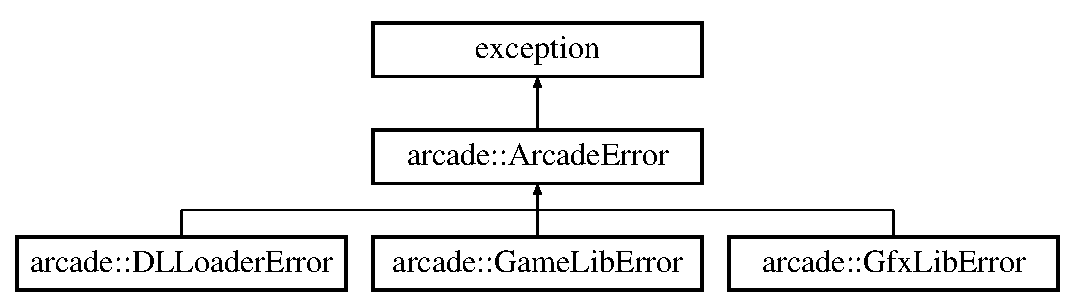
\includegraphics[height=3.000000cm]{classarcade_1_1_arcade_error}
\end{center}
\end{figure}
\subsection*{Public Member Functions}
\begin{DoxyCompactItemize}
\item 
virtual \hyperlink{classarcade_1_1_arcade_error_a421014734e82162258dca5ec2836d860}{$\sim$\+Arcade\+Error} ()  throw ()
\item 
\hyperlink{classarcade_1_1_arcade_error_ab8c1d2196492a10bb07177d1c5187322}{Arcade\+Error} (std\+::string const \&msg)  throw ()
\item 
virtual const char $\ast$ \hyperlink{classarcade_1_1_arcade_error_a48642ed78360efee13b4f1e343035f4e}{what} () const  throw ()
\end{DoxyCompactItemize}


\subsection{Constructor \& Destructor Documentation}
\mbox{\Hypertarget{classarcade_1_1_arcade_error_a421014734e82162258dca5ec2836d860}\label{classarcade_1_1_arcade_error_a421014734e82162258dca5ec2836d860}} 
\index{arcade\+::\+Arcade\+Error@{arcade\+::\+Arcade\+Error}!````~Arcade\+Error@{$\sim$\+Arcade\+Error}}
\index{````~Arcade\+Error@{$\sim$\+Arcade\+Error}!arcade\+::\+Arcade\+Error@{arcade\+::\+Arcade\+Error}}
\subsubsection{\texorpdfstring{$\sim$\+Arcade\+Error()}{~ArcadeError()}}
{\footnotesize\ttfamily arcade\+::\+Arcade\+Error\+::$\sim$\+Arcade\+Error (\begin{DoxyParamCaption}{ }\end{DoxyParamCaption}) throw  ) \hspace{0.3cm}{\ttfamily [virtual]}}

\mbox{\Hypertarget{classarcade_1_1_arcade_error_ab8c1d2196492a10bb07177d1c5187322}\label{classarcade_1_1_arcade_error_ab8c1d2196492a10bb07177d1c5187322}} 
\index{arcade\+::\+Arcade\+Error@{arcade\+::\+Arcade\+Error}!Arcade\+Error@{Arcade\+Error}}
\index{Arcade\+Error@{Arcade\+Error}!arcade\+::\+Arcade\+Error@{arcade\+::\+Arcade\+Error}}
\subsubsection{\texorpdfstring{Arcade\+Error()}{ArcadeError()}}
{\footnotesize\ttfamily arcade\+::\+Arcade\+Error\+::\+Arcade\+Error (\begin{DoxyParamCaption}\item[{std\+::string const \&}]{msg }\end{DoxyParamCaption}) throw  ) }



\subsection{Member Function Documentation}
\mbox{\Hypertarget{classarcade_1_1_arcade_error_a48642ed78360efee13b4f1e343035f4e}\label{classarcade_1_1_arcade_error_a48642ed78360efee13b4f1e343035f4e}} 
\index{arcade\+::\+Arcade\+Error@{arcade\+::\+Arcade\+Error}!what@{what}}
\index{what@{what}!arcade\+::\+Arcade\+Error@{arcade\+::\+Arcade\+Error}}
\subsubsection{\texorpdfstring{what()}{what()}}
{\footnotesize\ttfamily const char $\ast$ arcade\+::\+Arcade\+Error\+::what (\begin{DoxyParamCaption}{ }\end{DoxyParamCaption}) const throw  ) \hspace{0.3cm}{\ttfamily [virtual]}}



The documentation for this class was generated from the following files\+:\begin{DoxyCompactItemize}
\item 
include/\hyperlink{_exception_8hpp}{Exception.\+hpp}\item 
srcs/\hyperlink{_exception_8cpp}{Exception.\+cpp}\end{DoxyCompactItemize}

\hypertarget{structarcade_1_1_gfx_lapin_1_1bunny__window}{}\section{arcade\+:\+:Gfx\+Lapin\+:\+:bunny\+\_\+window Struct Reference}
\label{structarcade_1_1_gfx_lapin_1_1bunny__window}\index{arcade\+::\+Gfx\+Lapin\+::bunny\+\_\+window@{arcade\+::\+Gfx\+Lapin\+::bunny\+\_\+window}}


{\ttfamily \#include $<$Gfx\+Lapin.\+hpp$>$}

\subsection*{Public Attributes}
\begin{DoxyCompactItemize}
\item 
size\+\_\+t \hyperlink{structarcade_1_1_gfx_lapin_1_1bunny__window_a244ad1e472833f5778b301bb79b37b76}{type}
\item 
sf\+::\+Render\+Window $\ast$ \hyperlink{structarcade_1_1_gfx_lapin_1_1bunny__window_a9d397c64ed4b4d17df00cd4acddf5632}{window}
\item 
ssize\+\_\+t \hyperlink{structarcade_1_1_gfx_lapin_1_1bunny__window_afdc8b4dc731f6d51f596ea2d9a6ec9e9}{width}
\item 
ssize\+\_\+t \hyperlink{structarcade_1_1_gfx_lapin_1_1bunny__window_a8f57e2fcac1d4176524fdcbba4d968b2}{height}
\item 
const char $\ast$ \hyperlink{structarcade_1_1_gfx_lapin_1_1bunny__window_a9855e6af6789811f8ee718b615e22ee3}{window\+\_\+name}
\end{DoxyCompactItemize}


\subsection{Member Data Documentation}
\mbox{\Hypertarget{structarcade_1_1_gfx_lapin_1_1bunny__window_a8f57e2fcac1d4176524fdcbba4d968b2}\label{structarcade_1_1_gfx_lapin_1_1bunny__window_a8f57e2fcac1d4176524fdcbba4d968b2}} 
\index{arcade\+::\+Gfx\+Lapin\+::bunny\+\_\+window@{arcade\+::\+Gfx\+Lapin\+::bunny\+\_\+window}!height@{height}}
\index{height@{height}!arcade\+::\+Gfx\+Lapin\+::bunny\+\_\+window@{arcade\+::\+Gfx\+Lapin\+::bunny\+\_\+window}}
\subsubsection{\texorpdfstring{height}{height}}
{\footnotesize\ttfamily ssize\+\_\+t arcade\+::\+Gfx\+Lapin\+::bunny\+\_\+window\+::height}

\mbox{\Hypertarget{structarcade_1_1_gfx_lapin_1_1bunny__window_a244ad1e472833f5778b301bb79b37b76}\label{structarcade_1_1_gfx_lapin_1_1bunny__window_a244ad1e472833f5778b301bb79b37b76}} 
\index{arcade\+::\+Gfx\+Lapin\+::bunny\+\_\+window@{arcade\+::\+Gfx\+Lapin\+::bunny\+\_\+window}!type@{type}}
\index{type@{type}!arcade\+::\+Gfx\+Lapin\+::bunny\+\_\+window@{arcade\+::\+Gfx\+Lapin\+::bunny\+\_\+window}}
\subsubsection{\texorpdfstring{type}{type}}
{\footnotesize\ttfamily size\+\_\+t arcade\+::\+Gfx\+Lapin\+::bunny\+\_\+window\+::type}

\mbox{\Hypertarget{structarcade_1_1_gfx_lapin_1_1bunny__window_afdc8b4dc731f6d51f596ea2d9a6ec9e9}\label{structarcade_1_1_gfx_lapin_1_1bunny__window_afdc8b4dc731f6d51f596ea2d9a6ec9e9}} 
\index{arcade\+::\+Gfx\+Lapin\+::bunny\+\_\+window@{arcade\+::\+Gfx\+Lapin\+::bunny\+\_\+window}!width@{width}}
\index{width@{width}!arcade\+::\+Gfx\+Lapin\+::bunny\+\_\+window@{arcade\+::\+Gfx\+Lapin\+::bunny\+\_\+window}}
\subsubsection{\texorpdfstring{width}{width}}
{\footnotesize\ttfamily ssize\+\_\+t arcade\+::\+Gfx\+Lapin\+::bunny\+\_\+window\+::width}

\mbox{\Hypertarget{structarcade_1_1_gfx_lapin_1_1bunny__window_a9d397c64ed4b4d17df00cd4acddf5632}\label{structarcade_1_1_gfx_lapin_1_1bunny__window_a9d397c64ed4b4d17df00cd4acddf5632}} 
\index{arcade\+::\+Gfx\+Lapin\+::bunny\+\_\+window@{arcade\+::\+Gfx\+Lapin\+::bunny\+\_\+window}!window@{window}}
\index{window@{window}!arcade\+::\+Gfx\+Lapin\+::bunny\+\_\+window@{arcade\+::\+Gfx\+Lapin\+::bunny\+\_\+window}}
\subsubsection{\texorpdfstring{window}{window}}
{\footnotesize\ttfamily sf\+::\+Render\+Window$\ast$ arcade\+::\+Gfx\+Lapin\+::bunny\+\_\+window\+::window}

\mbox{\Hypertarget{structarcade_1_1_gfx_lapin_1_1bunny__window_a9855e6af6789811f8ee718b615e22ee3}\label{structarcade_1_1_gfx_lapin_1_1bunny__window_a9855e6af6789811f8ee718b615e22ee3}} 
\index{arcade\+::\+Gfx\+Lapin\+::bunny\+\_\+window@{arcade\+::\+Gfx\+Lapin\+::bunny\+\_\+window}!window\+\_\+name@{window\+\_\+name}}
\index{window\+\_\+name@{window\+\_\+name}!arcade\+::\+Gfx\+Lapin\+::bunny\+\_\+window@{arcade\+::\+Gfx\+Lapin\+::bunny\+\_\+window}}
\subsubsection{\texorpdfstring{window\+\_\+name}{window\_name}}
{\footnotesize\ttfamily const char$\ast$ arcade\+::\+Gfx\+Lapin\+::bunny\+\_\+window\+::window\+\_\+name}



The documentation for this struct was generated from the following file\+:\begin{DoxyCompactItemize}
\item 
gfx\+Libs\+Srcs/lapin/include/\hyperlink{_gfx_lapin_8hpp}{Gfx\+Lapin.\+hpp}\end{DoxyCompactItemize}

\hypertarget{unionarcade_1_1_color}{}\section{arcade\+:\+:Color Union Reference}
\label{unionarcade_1_1_color}\index{arcade\+::\+Color@{arcade\+::\+Color}}


Union to store R\+G\+Ba color.  




{\ttfamily \#include $<$Color.\+hpp$>$}

\subsection*{Public Member Functions}
\begin{DoxyCompactItemize}
\item 
\hyperlink{unionarcade_1_1_color_a053784aa4df3917111e2717d74fa3d85}{Color} (uint32\+\_\+t c=Black.\+full)
\begin{DoxyCompactList}\small\item\em Constructor to create color from a 4 bytes integer. \end{DoxyCompactList}\item 
\hyperlink{unionarcade_1_1_color_acf519d304c0dae64e28b976414af0753}{Color} (uint8\+\_\+t \hyperlink{unionarcade_1_1_color_a20637c0cb142a384bd034cceacafe6e0}{r}, uint8\+\_\+t \hyperlink{unionarcade_1_1_color_a97c509df99c9b119622f4b2ff8b3f21b}{g}, uint8\+\_\+t \hyperlink{unionarcade_1_1_color_a7edec98cabcfdeb71ae750e7442a6baf}{b}, uint8\+\_\+t \hyperlink{unionarcade_1_1_color_ae2f888f27d844d24f9ef10917f42d2dc}{a}=255)
\begin{DoxyCompactList}\small\item\em Constructor to create color from a 4 color component. \end{DoxyCompactList}\item 
\hyperlink{unionarcade_1_1_color_a25345f417c09d13da1b20f5a0f030eec}{Color} (\hyperlink{unionarcade_1_1_color}{Color} const \&c)
\begin{DoxyCompactList}\small\item\em Constructor to copy a \hyperlink{unionarcade_1_1_color}{Color}. \end{DoxyCompactList}\end{DoxyCompactItemize}
\subsection*{Public Attributes}
\begin{DoxyCompactItemize}
\item 
uint32\+\_\+t \hyperlink{unionarcade_1_1_color_ad68cc4b72cafa2c89dac97a336d1ca32}{full}
\begin{DoxyCompactList}\small\item\em Transparent color. \end{DoxyCompactList}\item 
uint8\+\_\+t \hyperlink{unionarcade_1_1_color_a805bb231543d607ee00f353506c850be}{rgba} \mbox{[}4\mbox{]}
\begin{DoxyCompactList}\small\item\em 4 bytes integer value of the color \end{DoxyCompactList}\item 
\begin{tabbing}
xx\=xx\=xx\=xx\=xx\=xx\=xx\=xx\=xx\=\kill
struct \{\\
\>uint8\_t \hyperlink{unionarcade_1_1_color_a20637c0cb142a384bd034cceacafe6e0}{r}\\
\>uint8\_t \hyperlink{unionarcade_1_1_color_a97c509df99c9b119622f4b2ff8b3f21b}{g}\\
\>uint8\_t \hyperlink{unionarcade_1_1_color_a7edec98cabcfdeb71ae750e7442a6baf}{b}\\
\>uint8\_t \hyperlink{unionarcade_1_1_color_ae2f888f27d844d24f9ef10917f42d2dc}{a}\\
\}; \\

\end{tabbing}\begin{DoxyCompactList}\small\item\em array of the 4 color component \end{DoxyCompactList}\end{DoxyCompactItemize}
\subsection*{Static Public Attributes}
\begin{DoxyCompactItemize}
\item 
static const \hyperlink{unionarcade_1_1_color}{Color} \hyperlink{unionarcade_1_1_color_adf9314b9d80e839db37907dc8e281175}{Black}
\item 
static const \hyperlink{unionarcade_1_1_color}{Color} \hyperlink{unionarcade_1_1_color_aa8bd809fbf902dbbe53b9bb6802eb57f}{White}
\begin{DoxyCompactList}\small\item\em Black color. \end{DoxyCompactList}\item 
static const \hyperlink{unionarcade_1_1_color}{Color} \hyperlink{unionarcade_1_1_color_a7101e34126fdb3c14d53045681938293}{Red}
\begin{DoxyCompactList}\small\item\em White color. \end{DoxyCompactList}\item 
static const \hyperlink{unionarcade_1_1_color}{Color} \hyperlink{unionarcade_1_1_color_aa7271d3c9e5fc07926979eaa610af7e4}{Green}
\begin{DoxyCompactList}\small\item\em Red color. \end{DoxyCompactList}\item 
static const \hyperlink{unionarcade_1_1_color}{Color} \hyperlink{unionarcade_1_1_color_a37e72a85b3ce04f4642a48cae2f60644}{Blue}
\begin{DoxyCompactList}\small\item\em Green color. \end{DoxyCompactList}\item 
static const \hyperlink{unionarcade_1_1_color}{Color} \hyperlink{unionarcade_1_1_color_aa437de4029652dba87b0b64ca488f8ff}{Yellow}
\begin{DoxyCompactList}\small\item\em Blue color. \end{DoxyCompactList}\item 
static const \hyperlink{unionarcade_1_1_color}{Color} \hyperlink{unionarcade_1_1_color_aabfdd84cadc61ca458e8122869310631}{Magenta}
\begin{DoxyCompactList}\small\item\em Yellow color. \end{DoxyCompactList}\item 
static const \hyperlink{unionarcade_1_1_color}{Color} \hyperlink{unionarcade_1_1_color_a73cbdbe2ebf731489bafec16cb88e705}{Cyan}
\begin{DoxyCompactList}\small\item\em Magenta color. \end{DoxyCompactList}\item 
static const \hyperlink{unionarcade_1_1_color}{Color} \hyperlink{unionarcade_1_1_color_a689350442a28301beb49ca78a4885e4f}{Transparent}
\begin{DoxyCompactList}\small\item\em Cyan color. \end{DoxyCompactList}\end{DoxyCompactItemize}


\subsection{Detailed Description}
Union to store R\+G\+Ba color. 

\subsection{Constructor \& Destructor Documentation}
\mbox{\Hypertarget{unionarcade_1_1_color_a053784aa4df3917111e2717d74fa3d85}\label{unionarcade_1_1_color_a053784aa4df3917111e2717d74fa3d85}} 
\index{arcade\+::\+Color@{arcade\+::\+Color}!Color@{Color}}
\index{Color@{Color}!arcade\+::\+Color@{arcade\+::\+Color}}
\subsubsection{\texorpdfstring{Color()}{Color()}\hspace{0.1cm}{\footnotesize\ttfamily [1/3]}}
{\footnotesize\ttfamily arcade\+::\+Color\+::\+Color (\begin{DoxyParamCaption}\item[{uint32\+\_\+t}]{c = {\ttfamily Black.full} }\end{DoxyParamCaption})}



Constructor to create color from a 4 bytes integer. 


\begin{DoxyParams}[1]{Parameters}
\mbox{\tt in}  & {\em c} & 4 bytes integer value containing a color \\
\hline
\end{DoxyParams}
\mbox{\Hypertarget{unionarcade_1_1_color_acf519d304c0dae64e28b976414af0753}\label{unionarcade_1_1_color_acf519d304c0dae64e28b976414af0753}} 
\index{arcade\+::\+Color@{arcade\+::\+Color}!Color@{Color}}
\index{Color@{Color}!arcade\+::\+Color@{arcade\+::\+Color}}
\subsubsection{\texorpdfstring{Color()}{Color()}\hspace{0.1cm}{\footnotesize\ttfamily [2/3]}}
{\footnotesize\ttfamily arcade\+::\+Color\+::\+Color (\begin{DoxyParamCaption}\item[{uint8\+\_\+t}]{r,  }\item[{uint8\+\_\+t}]{g,  }\item[{uint8\+\_\+t}]{b,  }\item[{uint8\+\_\+t}]{a = {\ttfamily 255} }\end{DoxyParamCaption})}



Constructor to create color from a 4 color component. 


\begin{DoxyParams}[1]{Parameters}
\mbox{\tt in}  & {\em r} & Red color component value \\
\hline
\mbox{\tt in}  & {\em g} & Green color component value \\
\hline
\mbox{\tt in}  & {\em b} & Blue color component value \\
\hline
\mbox{\tt in}  & {\em a} & Alpha (opacity) color component value \\
\hline
\end{DoxyParams}
\mbox{\Hypertarget{unionarcade_1_1_color_a25345f417c09d13da1b20f5a0f030eec}\label{unionarcade_1_1_color_a25345f417c09d13da1b20f5a0f030eec}} 
\index{arcade\+::\+Color@{arcade\+::\+Color}!Color@{Color}}
\index{Color@{Color}!arcade\+::\+Color@{arcade\+::\+Color}}
\subsubsection{\texorpdfstring{Color()}{Color()}\hspace{0.1cm}{\footnotesize\ttfamily [3/3]}}
{\footnotesize\ttfamily arcade\+::\+Color\+::\+Color (\begin{DoxyParamCaption}\item[{\hyperlink{unionarcade_1_1_color}{Color} const \&}]{c }\end{DoxyParamCaption})}



Constructor to copy a \hyperlink{unionarcade_1_1_color}{Color}. 


\begin{DoxyParams}[1]{Parameters}
\mbox{\tt in}  & {\em c} & \hyperlink{unionarcade_1_1_color}{Color} to be copied \\
\hline
\end{DoxyParams}


\subsection{Member Data Documentation}
\mbox{\Hypertarget{unionarcade_1_1_color_a43cc3c8f8963922521042f4ea70178b3}\label{unionarcade_1_1_color_a43cc3c8f8963922521042f4ea70178b3}} 
\subsubsection{\texorpdfstring{"@1}{@1}}
{\footnotesize\ttfamily struct \{ ... \} }



array of the 4 color component 

\mbox{\Hypertarget{unionarcade_1_1_color_ae2f888f27d844d24f9ef10917f42d2dc}\label{unionarcade_1_1_color_ae2f888f27d844d24f9ef10917f42d2dc}} 
\index{arcade\+::\+Color@{arcade\+::\+Color}!a@{a}}
\index{a@{a}!arcade\+::\+Color@{arcade\+::\+Color}}
\subsubsection{\texorpdfstring{a}{a}}
{\footnotesize\ttfamily uint8\+\_\+t arcade\+::\+Color\+::a}

\mbox{\Hypertarget{unionarcade_1_1_color_a7edec98cabcfdeb71ae750e7442a6baf}\label{unionarcade_1_1_color_a7edec98cabcfdeb71ae750e7442a6baf}} 
\index{arcade\+::\+Color@{arcade\+::\+Color}!b@{b}}
\index{b@{b}!arcade\+::\+Color@{arcade\+::\+Color}}
\subsubsection{\texorpdfstring{b}{b}}
{\footnotesize\ttfamily uint8\+\_\+t arcade\+::\+Color\+::b}

\mbox{\Hypertarget{unionarcade_1_1_color_adf9314b9d80e839db37907dc8e281175}\label{unionarcade_1_1_color_adf9314b9d80e839db37907dc8e281175}} 
\index{arcade\+::\+Color@{arcade\+::\+Color}!Black@{Black}}
\index{Black@{Black}!arcade\+::\+Color@{arcade\+::\+Color}}
\subsubsection{\texorpdfstring{Black}{Black}}
{\footnotesize\ttfamily const \hyperlink{unionarcade_1_1_color}{Color} arcade\+::\+Color\+::\+Black\hspace{0.3cm}{\ttfamily [static]}}

\mbox{\Hypertarget{unionarcade_1_1_color_a37e72a85b3ce04f4642a48cae2f60644}\label{unionarcade_1_1_color_a37e72a85b3ce04f4642a48cae2f60644}} 
\index{arcade\+::\+Color@{arcade\+::\+Color}!Blue@{Blue}}
\index{Blue@{Blue}!arcade\+::\+Color@{arcade\+::\+Color}}
\subsubsection{\texorpdfstring{Blue}{Blue}}
{\footnotesize\ttfamily const \hyperlink{unionarcade_1_1_color}{Color} arcade\+::\+Color\+::\+Blue\hspace{0.3cm}{\ttfamily [static]}}



Green color. 

\mbox{\Hypertarget{unionarcade_1_1_color_a73cbdbe2ebf731489bafec16cb88e705}\label{unionarcade_1_1_color_a73cbdbe2ebf731489bafec16cb88e705}} 
\index{arcade\+::\+Color@{arcade\+::\+Color}!Cyan@{Cyan}}
\index{Cyan@{Cyan}!arcade\+::\+Color@{arcade\+::\+Color}}
\subsubsection{\texorpdfstring{Cyan}{Cyan}}
{\footnotesize\ttfamily const \hyperlink{unionarcade_1_1_color}{Color} arcade\+::\+Color\+::\+Cyan\hspace{0.3cm}{\ttfamily [static]}}



Magenta color. 

\mbox{\Hypertarget{unionarcade_1_1_color_ad68cc4b72cafa2c89dac97a336d1ca32}\label{unionarcade_1_1_color_ad68cc4b72cafa2c89dac97a336d1ca32}} 
\index{arcade\+::\+Color@{arcade\+::\+Color}!full@{full}}
\index{full@{full}!arcade\+::\+Color@{arcade\+::\+Color}}
\subsubsection{\texorpdfstring{full}{full}}
{\footnotesize\ttfamily uint32\+\_\+t arcade\+::\+Color\+::full}



Transparent color. 

\mbox{\Hypertarget{unionarcade_1_1_color_a97c509df99c9b119622f4b2ff8b3f21b}\label{unionarcade_1_1_color_a97c509df99c9b119622f4b2ff8b3f21b}} 
\index{arcade\+::\+Color@{arcade\+::\+Color}!g@{g}}
\index{g@{g}!arcade\+::\+Color@{arcade\+::\+Color}}
\subsubsection{\texorpdfstring{g}{g}}
{\footnotesize\ttfamily uint8\+\_\+t arcade\+::\+Color\+::g}

\mbox{\Hypertarget{unionarcade_1_1_color_aa7271d3c9e5fc07926979eaa610af7e4}\label{unionarcade_1_1_color_aa7271d3c9e5fc07926979eaa610af7e4}} 
\index{arcade\+::\+Color@{arcade\+::\+Color}!Green@{Green}}
\index{Green@{Green}!arcade\+::\+Color@{arcade\+::\+Color}}
\subsubsection{\texorpdfstring{Green}{Green}}
{\footnotesize\ttfamily const \hyperlink{unionarcade_1_1_color}{Color} arcade\+::\+Color\+::\+Green\hspace{0.3cm}{\ttfamily [static]}}



Red color. 

\mbox{\Hypertarget{unionarcade_1_1_color_aabfdd84cadc61ca458e8122869310631}\label{unionarcade_1_1_color_aabfdd84cadc61ca458e8122869310631}} 
\index{arcade\+::\+Color@{arcade\+::\+Color}!Magenta@{Magenta}}
\index{Magenta@{Magenta}!arcade\+::\+Color@{arcade\+::\+Color}}
\subsubsection{\texorpdfstring{Magenta}{Magenta}}
{\footnotesize\ttfamily const \hyperlink{unionarcade_1_1_color}{Color} arcade\+::\+Color\+::\+Magenta\hspace{0.3cm}{\ttfamily [static]}}



Yellow color. 

\mbox{\Hypertarget{unionarcade_1_1_color_a20637c0cb142a384bd034cceacafe6e0}\label{unionarcade_1_1_color_a20637c0cb142a384bd034cceacafe6e0}} 
\index{arcade\+::\+Color@{arcade\+::\+Color}!r@{r}}
\index{r@{r}!arcade\+::\+Color@{arcade\+::\+Color}}
\subsubsection{\texorpdfstring{r}{r}}
{\footnotesize\ttfamily uint8\+\_\+t arcade\+::\+Color\+::r}

\mbox{\Hypertarget{unionarcade_1_1_color_a7101e34126fdb3c14d53045681938293}\label{unionarcade_1_1_color_a7101e34126fdb3c14d53045681938293}} 
\index{arcade\+::\+Color@{arcade\+::\+Color}!Red@{Red}}
\index{Red@{Red}!arcade\+::\+Color@{arcade\+::\+Color}}
\subsubsection{\texorpdfstring{Red}{Red}}
{\footnotesize\ttfamily const \hyperlink{unionarcade_1_1_color}{Color} arcade\+::\+Color\+::\+Red\hspace{0.3cm}{\ttfamily [static]}}



White color. 

\mbox{\Hypertarget{unionarcade_1_1_color_a805bb231543d607ee00f353506c850be}\label{unionarcade_1_1_color_a805bb231543d607ee00f353506c850be}} 
\index{arcade\+::\+Color@{arcade\+::\+Color}!rgba@{rgba}}
\index{rgba@{rgba}!arcade\+::\+Color@{arcade\+::\+Color}}
\subsubsection{\texorpdfstring{rgba}{rgba}}
{\footnotesize\ttfamily uint8\+\_\+t arcade\+::\+Color\+::rgba\mbox{[}4\mbox{]}}



4 bytes integer value of the color 

\mbox{\Hypertarget{unionarcade_1_1_color_a689350442a28301beb49ca78a4885e4f}\label{unionarcade_1_1_color_a689350442a28301beb49ca78a4885e4f}} 
\index{arcade\+::\+Color@{arcade\+::\+Color}!Transparent@{Transparent}}
\index{Transparent@{Transparent}!arcade\+::\+Color@{arcade\+::\+Color}}
\subsubsection{\texorpdfstring{Transparent}{Transparent}}
{\footnotesize\ttfamily const \hyperlink{unionarcade_1_1_color}{Color} arcade\+::\+Color\+::\+Transparent\hspace{0.3cm}{\ttfamily [static]}}



Cyan color. 

\mbox{\Hypertarget{unionarcade_1_1_color_aa8bd809fbf902dbbe53b9bb6802eb57f}\label{unionarcade_1_1_color_aa8bd809fbf902dbbe53b9bb6802eb57f}} 
\index{arcade\+::\+Color@{arcade\+::\+Color}!White@{White}}
\index{White@{White}!arcade\+::\+Color@{arcade\+::\+Color}}
\subsubsection{\texorpdfstring{White}{White}}
{\footnotesize\ttfamily const \hyperlink{unionarcade_1_1_color}{Color} arcade\+::\+Color\+::\+White\hspace{0.3cm}{\ttfamily [static]}}



Black color. 

\mbox{\Hypertarget{unionarcade_1_1_color_aa437de4029652dba87b0b64ca488f8ff}\label{unionarcade_1_1_color_aa437de4029652dba87b0b64ca488f8ff}} 
\index{arcade\+::\+Color@{arcade\+::\+Color}!Yellow@{Yellow}}
\index{Yellow@{Yellow}!arcade\+::\+Color@{arcade\+::\+Color}}
\subsubsection{\texorpdfstring{Yellow}{Yellow}}
{\footnotesize\ttfamily const \hyperlink{unionarcade_1_1_color}{Color} arcade\+::\+Color\+::\+Yellow\hspace{0.3cm}{\ttfamily [static]}}



Blue color. 



The documentation for this union was generated from the following files\+:\begin{DoxyCompactItemize}
\item 
arcade\+Interfaces/\hyperlink{_color_8hpp}{Color.\+hpp}\item 
arcade\+Interfaces/\hyperlink{_color_8cpp}{Color.\+cpp}\end{DoxyCompactItemize}

\hypertarget{classarcade_1_1_core}{}\section{arcade\+:\+:Core Class Reference}
\label{classarcade_1_1_core}\index{arcade\+::\+Core@{arcade\+::\+Core}}


{\ttfamily \#include $<$Core.\+hpp$>$}

\subsection*{Public Member Functions}
\begin{DoxyCompactItemize}
\item 
virtual \hyperlink{classarcade_1_1_core_a4a80f4851276173b3055fc41268d3b3d}{$\sim$\+Core} ()
\item 
\hyperlink{classarcade_1_1_core_a2d707a14ea555e2b72fb6fb4a6ad0305}{Core} (std\+::string const \&path\+To\+Lib)
\item 
void \hyperlink{classarcade_1_1_core_a93f9b90157e2fd1d4020542e17864280}{load\+Gfx\+Lib} (std\+::string const \&path\+To\+Lib)
\item 
void \hyperlink{classarcade_1_1_core_acbda8d28b646429b74b94e0e87ea8620}{load\+Game\+Lib} (std\+::string const \&path\+To\+Game)
\item 
void \hyperlink{classarcade_1_1_core_a1fd3e057f1a020bd61a074bb2143bac7}{core\+Loop} ()
\item 
void \hyperlink{classarcade_1_1_core_a60fbdf58db50c1ab65c3f31d02f5d3d3}{prev\+Game} ()
\item 
void \hyperlink{classarcade_1_1_core_a7147bc7c0a9f184ea2237848d2bfd570}{next\+Game} ()
\item 
void \hyperlink{classarcade_1_1_core_a080c95e72cb95b887ca959f1a07a885e}{prev\+Gfx\+Lib} ()
\item 
void \hyperlink{classarcade_1_1_core_a8e9e31b7c6313edf31fe7a44af4b01d1}{next\+Gfx\+Lib} ()
\item 
void \hyperlink{classarcade_1_1_core_a5393143a3668f07126a6f20c12f0fa9a}{restart\+Game} ()
\item 
void \hyperlink{classarcade_1_1_core_a2785108b212f43d686484d514478f238}{back\+To\+Menu} ()
\end{DoxyCompactItemize}


\subsection{Constructor \& Destructor Documentation}
\mbox{\Hypertarget{classarcade_1_1_core_a4a80f4851276173b3055fc41268d3b3d}\label{classarcade_1_1_core_a4a80f4851276173b3055fc41268d3b3d}} 
\index{arcade\+::\+Core@{arcade\+::\+Core}!````~Core@{$\sim$\+Core}}
\index{````~Core@{$\sim$\+Core}!arcade\+::\+Core@{arcade\+::\+Core}}
\subsubsection{\texorpdfstring{$\sim$\+Core()}{~Core()}}
{\footnotesize\ttfamily arcade\+::\+Core\+::$\sim$\+Core (\begin{DoxyParamCaption}{ }\end{DoxyParamCaption})\hspace{0.3cm}{\ttfamily [virtual]}}

\mbox{\Hypertarget{classarcade_1_1_core_a2d707a14ea555e2b72fb6fb4a6ad0305}\label{classarcade_1_1_core_a2d707a14ea555e2b72fb6fb4a6ad0305}} 
\index{arcade\+::\+Core@{arcade\+::\+Core}!Core@{Core}}
\index{Core@{Core}!arcade\+::\+Core@{arcade\+::\+Core}}
\subsubsection{\texorpdfstring{Core()}{Core()}}
{\footnotesize\ttfamily arcade\+::\+Core\+::\+Core (\begin{DoxyParamCaption}\item[{std\+::string const \&}]{path\+To\+Lib }\end{DoxyParamCaption})}



\subsection{Member Function Documentation}
\mbox{\Hypertarget{classarcade_1_1_core_a2785108b212f43d686484d514478f238}\label{classarcade_1_1_core_a2785108b212f43d686484d514478f238}} 
\index{arcade\+::\+Core@{arcade\+::\+Core}!back\+To\+Menu@{back\+To\+Menu}}
\index{back\+To\+Menu@{back\+To\+Menu}!arcade\+::\+Core@{arcade\+::\+Core}}
\subsubsection{\texorpdfstring{back\+To\+Menu()}{backToMenu()}}
{\footnotesize\ttfamily void arcade\+::\+Core\+::back\+To\+Menu (\begin{DoxyParamCaption}{ }\end{DoxyParamCaption})}

\mbox{\Hypertarget{classarcade_1_1_core_a1fd3e057f1a020bd61a074bb2143bac7}\label{classarcade_1_1_core_a1fd3e057f1a020bd61a074bb2143bac7}} 
\index{arcade\+::\+Core@{arcade\+::\+Core}!core\+Loop@{core\+Loop}}
\index{core\+Loop@{core\+Loop}!arcade\+::\+Core@{arcade\+::\+Core}}
\subsubsection{\texorpdfstring{core\+Loop()}{coreLoop()}}
{\footnotesize\ttfamily void arcade\+::\+Core\+::core\+Loop (\begin{DoxyParamCaption}{ }\end{DoxyParamCaption})}

\mbox{\Hypertarget{classarcade_1_1_core_acbda8d28b646429b74b94e0e87ea8620}\label{classarcade_1_1_core_acbda8d28b646429b74b94e0e87ea8620}} 
\index{arcade\+::\+Core@{arcade\+::\+Core}!load\+Game\+Lib@{load\+Game\+Lib}}
\index{load\+Game\+Lib@{load\+Game\+Lib}!arcade\+::\+Core@{arcade\+::\+Core}}
\subsubsection{\texorpdfstring{load\+Game\+Lib()}{loadGameLib()}}
{\footnotesize\ttfamily void arcade\+::\+Core\+::load\+Game\+Lib (\begin{DoxyParamCaption}\item[{std\+::string const \&}]{path\+To\+Game }\end{DoxyParamCaption})}

\mbox{\Hypertarget{classarcade_1_1_core_a93f9b90157e2fd1d4020542e17864280}\label{classarcade_1_1_core_a93f9b90157e2fd1d4020542e17864280}} 
\index{arcade\+::\+Core@{arcade\+::\+Core}!load\+Gfx\+Lib@{load\+Gfx\+Lib}}
\index{load\+Gfx\+Lib@{load\+Gfx\+Lib}!arcade\+::\+Core@{arcade\+::\+Core}}
\subsubsection{\texorpdfstring{load\+Gfx\+Lib()}{loadGfxLib()}}
{\footnotesize\ttfamily void arcade\+::\+Core\+::load\+Gfx\+Lib (\begin{DoxyParamCaption}\item[{std\+::string const \&}]{path\+To\+Lib }\end{DoxyParamCaption})}

\mbox{\Hypertarget{classarcade_1_1_core_a7147bc7c0a9f184ea2237848d2bfd570}\label{classarcade_1_1_core_a7147bc7c0a9f184ea2237848d2bfd570}} 
\index{arcade\+::\+Core@{arcade\+::\+Core}!next\+Game@{next\+Game}}
\index{next\+Game@{next\+Game}!arcade\+::\+Core@{arcade\+::\+Core}}
\subsubsection{\texorpdfstring{next\+Game()}{nextGame()}}
{\footnotesize\ttfamily void arcade\+::\+Core\+::next\+Game (\begin{DoxyParamCaption}{ }\end{DoxyParamCaption})}

\mbox{\Hypertarget{classarcade_1_1_core_a8e9e31b7c6313edf31fe7a44af4b01d1}\label{classarcade_1_1_core_a8e9e31b7c6313edf31fe7a44af4b01d1}} 
\index{arcade\+::\+Core@{arcade\+::\+Core}!next\+Gfx\+Lib@{next\+Gfx\+Lib}}
\index{next\+Gfx\+Lib@{next\+Gfx\+Lib}!arcade\+::\+Core@{arcade\+::\+Core}}
\subsubsection{\texorpdfstring{next\+Gfx\+Lib()}{nextGfxLib()}}
{\footnotesize\ttfamily void arcade\+::\+Core\+::next\+Gfx\+Lib (\begin{DoxyParamCaption}{ }\end{DoxyParamCaption})}

\mbox{\Hypertarget{classarcade_1_1_core_a60fbdf58db50c1ab65c3f31d02f5d3d3}\label{classarcade_1_1_core_a60fbdf58db50c1ab65c3f31d02f5d3d3}} 
\index{arcade\+::\+Core@{arcade\+::\+Core}!prev\+Game@{prev\+Game}}
\index{prev\+Game@{prev\+Game}!arcade\+::\+Core@{arcade\+::\+Core}}
\subsubsection{\texorpdfstring{prev\+Game()}{prevGame()}}
{\footnotesize\ttfamily void arcade\+::\+Core\+::prev\+Game (\begin{DoxyParamCaption}{ }\end{DoxyParamCaption})}

\mbox{\Hypertarget{classarcade_1_1_core_a080c95e72cb95b887ca959f1a07a885e}\label{classarcade_1_1_core_a080c95e72cb95b887ca959f1a07a885e}} 
\index{arcade\+::\+Core@{arcade\+::\+Core}!prev\+Gfx\+Lib@{prev\+Gfx\+Lib}}
\index{prev\+Gfx\+Lib@{prev\+Gfx\+Lib}!arcade\+::\+Core@{arcade\+::\+Core}}
\subsubsection{\texorpdfstring{prev\+Gfx\+Lib()}{prevGfxLib()}}
{\footnotesize\ttfamily void arcade\+::\+Core\+::prev\+Gfx\+Lib (\begin{DoxyParamCaption}{ }\end{DoxyParamCaption})}

\mbox{\Hypertarget{classarcade_1_1_core_a5393143a3668f07126a6f20c12f0fa9a}\label{classarcade_1_1_core_a5393143a3668f07126a6f20c12f0fa9a}} 
\index{arcade\+::\+Core@{arcade\+::\+Core}!restart\+Game@{restart\+Game}}
\index{restart\+Game@{restart\+Game}!arcade\+::\+Core@{arcade\+::\+Core}}
\subsubsection{\texorpdfstring{restart\+Game()}{restartGame()}}
{\footnotesize\ttfamily void arcade\+::\+Core\+::restart\+Game (\begin{DoxyParamCaption}{ }\end{DoxyParamCaption})}



The documentation for this class was generated from the following files\+:\begin{DoxyCompactItemize}
\item 
include/\hyperlink{_core_8hpp}{Core.\+hpp}\item 
srcs/\hyperlink{_core_8cpp}{Core.\+cpp}\end{DoxyCompactItemize}

\hypertarget{class_d_l_loader}{}\section{D\+L\+Loader$<$ T $>$ Class Template Reference}
\label{class_d_l_loader}\index{D\+L\+Loader$<$ T $>$@{D\+L\+Loader$<$ T $>$}}


{\ttfamily \#include $<$D\+L\+Loader.\+hpp$>$}

\subsection*{Public Member Functions}
\begin{DoxyCompactItemize}
\item 
\hyperlink{class_d_l_loader_a07bb2898993398632561704ffc3e4fc2}{D\+L\+Loader} (std\+::string const \&lib)
\item 
virtual \hyperlink{class_d_l_loader_aea867b497cf92c50f85ad7e1d37962ae}{$\sim$\+D\+L\+Loader} ()
\item 
T $\ast$ \hyperlink{class_d_l_loader_a27e0859099bf3bc981ee615078bc1c2f}{get\+Instance} (std\+::string const \&class\+Entry\+Point)
\item 
void \hyperlink{class_d_l_loader_acdd8ffa8f550ca1abe29bc1b24dc9914}{delete\+Instance} ()
\end{DoxyCompactItemize}


\subsection{Constructor \& Destructor Documentation}
\mbox{\Hypertarget{class_d_l_loader_a07bb2898993398632561704ffc3e4fc2}\label{class_d_l_loader_a07bb2898993398632561704ffc3e4fc2}} 
\index{D\+L\+Loader@{D\+L\+Loader}!D\+L\+Loader@{D\+L\+Loader}}
\index{D\+L\+Loader@{D\+L\+Loader}!D\+L\+Loader@{D\+L\+Loader}}
\subsubsection{\texorpdfstring{D\+L\+Loader()}{DLLoader()}}
{\footnotesize\ttfamily template$<$typename T $>$ \\
\hyperlink{class_d_l_loader}{D\+L\+Loader}$<$ T $>$\+::\hyperlink{class_d_l_loader}{D\+L\+Loader} (\begin{DoxyParamCaption}\item[{std\+::string const \&}]{lib }\end{DoxyParamCaption})}

\mbox{\Hypertarget{class_d_l_loader_aea867b497cf92c50f85ad7e1d37962ae}\label{class_d_l_loader_aea867b497cf92c50f85ad7e1d37962ae}} 
\index{D\+L\+Loader@{D\+L\+Loader}!````~D\+L\+Loader@{$\sim$\+D\+L\+Loader}}
\index{````~D\+L\+Loader@{$\sim$\+D\+L\+Loader}!D\+L\+Loader@{D\+L\+Loader}}
\subsubsection{\texorpdfstring{$\sim$\+D\+L\+Loader()}{~DLLoader()}}
{\footnotesize\ttfamily template$<$typename T $>$ \\
\hyperlink{class_d_l_loader}{D\+L\+Loader}$<$ T $>$\+::$\sim$\hyperlink{class_d_l_loader}{D\+L\+Loader} (\begin{DoxyParamCaption}{ }\end{DoxyParamCaption})\hspace{0.3cm}{\ttfamily [virtual]}}



\subsection{Member Function Documentation}
\mbox{\Hypertarget{class_d_l_loader_acdd8ffa8f550ca1abe29bc1b24dc9914}\label{class_d_l_loader_acdd8ffa8f550ca1abe29bc1b24dc9914}} 
\index{D\+L\+Loader@{D\+L\+Loader}!delete\+Instance@{delete\+Instance}}
\index{delete\+Instance@{delete\+Instance}!D\+L\+Loader@{D\+L\+Loader}}
\subsubsection{\texorpdfstring{delete\+Instance()}{deleteInstance()}}
{\footnotesize\ttfamily template$<$typename T$>$ \\
void \hyperlink{class_d_l_loader}{D\+L\+Loader}$<$ T $>$\+::delete\+Instance (\begin{DoxyParamCaption}{ }\end{DoxyParamCaption})}

\mbox{\Hypertarget{class_d_l_loader_a27e0859099bf3bc981ee615078bc1c2f}\label{class_d_l_loader_a27e0859099bf3bc981ee615078bc1c2f}} 
\index{D\+L\+Loader@{D\+L\+Loader}!get\+Instance@{get\+Instance}}
\index{get\+Instance@{get\+Instance}!D\+L\+Loader@{D\+L\+Loader}}
\subsubsection{\texorpdfstring{get\+Instance()}{getInstance()}}
{\footnotesize\ttfamily template$<$typename T $>$ \\
T $\ast$ \hyperlink{class_d_l_loader}{D\+L\+Loader}$<$ T $>$\+::get\+Instance (\begin{DoxyParamCaption}\item[{std\+::string const \&}]{class\+Entry\+Point }\end{DoxyParamCaption})}



The documentation for this class was generated from the following file\+:\begin{DoxyCompactItemize}
\item 
include/\hyperlink{_d_l_loader_8hpp}{D\+L\+Loader.\+hpp}\end{DoxyCompactItemize}

\hypertarget{classarcade_1_1_d_l_loader_error}{}\section{arcade\+:\+:D\+L\+Loader\+Error Class Reference}
\label{classarcade_1_1_d_l_loader_error}\index{arcade\+::\+D\+L\+Loader\+Error@{arcade\+::\+D\+L\+Loader\+Error}}


{\ttfamily \#include $<$Exception.\+hpp$>$}

Inheritance diagram for arcade\+:\+:D\+L\+Loader\+Error\+:\begin{figure}[H]
\begin{center}
\leavevmode
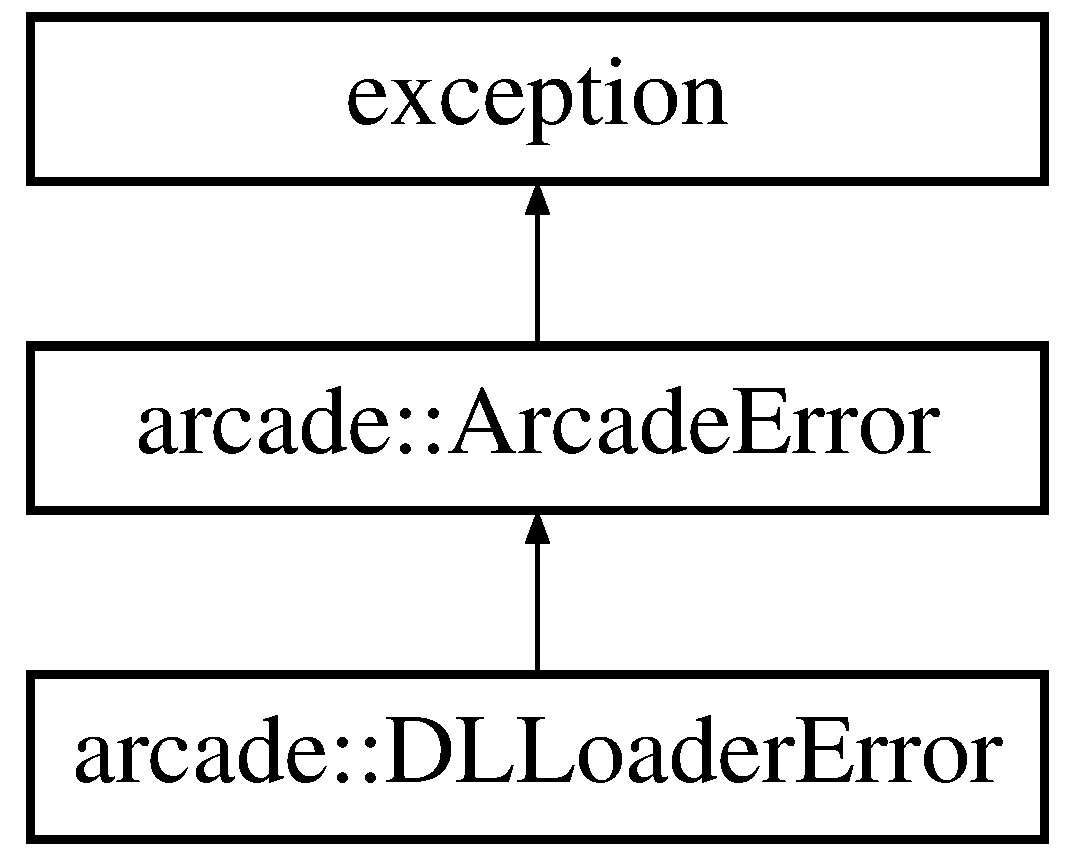
\includegraphics[height=3.000000cm]{classarcade_1_1_d_l_loader_error}
\end{center}
\end{figure}
\subsection*{Public Member Functions}
\begin{DoxyCompactItemize}
\item 
virtual \hyperlink{classarcade_1_1_d_l_loader_error_aa5f76a44c1fcddd0767cde52e19193b6}{$\sim$\+D\+L\+Loader\+Error} ()  throw ()
\item 
\hyperlink{classarcade_1_1_d_l_loader_error_a24f7cd1e5f5e897e535e0219802edb0d}{D\+L\+Loader\+Error} (const std\+::string \&msg)  throw ()
\end{DoxyCompactItemize}


\subsection{Constructor \& Destructor Documentation}
\mbox{\Hypertarget{classarcade_1_1_d_l_loader_error_aa5f76a44c1fcddd0767cde52e19193b6}\label{classarcade_1_1_d_l_loader_error_aa5f76a44c1fcddd0767cde52e19193b6}} 
\index{arcade\+::\+D\+L\+Loader\+Error@{arcade\+::\+D\+L\+Loader\+Error}!````~D\+L\+Loader\+Error@{$\sim$\+D\+L\+Loader\+Error}}
\index{````~D\+L\+Loader\+Error@{$\sim$\+D\+L\+Loader\+Error}!arcade\+::\+D\+L\+Loader\+Error@{arcade\+::\+D\+L\+Loader\+Error}}
\subsubsection{\texorpdfstring{$\sim$\+D\+L\+Loader\+Error()}{~DLLoaderError()}}
{\footnotesize\ttfamily arcade\+::\+D\+L\+Loader\+Error\+::$\sim$\+D\+L\+Loader\+Error (\begin{DoxyParamCaption}{ }\end{DoxyParamCaption}) throw  ) \hspace{0.3cm}{\ttfamily [virtual]}}

\mbox{\Hypertarget{classarcade_1_1_d_l_loader_error_a24f7cd1e5f5e897e535e0219802edb0d}\label{classarcade_1_1_d_l_loader_error_a24f7cd1e5f5e897e535e0219802edb0d}} 
\index{arcade\+::\+D\+L\+Loader\+Error@{arcade\+::\+D\+L\+Loader\+Error}!D\+L\+Loader\+Error@{D\+L\+Loader\+Error}}
\index{D\+L\+Loader\+Error@{D\+L\+Loader\+Error}!arcade\+::\+D\+L\+Loader\+Error@{arcade\+::\+D\+L\+Loader\+Error}}
\subsubsection{\texorpdfstring{D\+L\+Loader\+Error()}{DLLoaderError()}}
{\footnotesize\ttfamily arcade\+::\+D\+L\+Loader\+Error\+::\+D\+L\+Loader\+Error (\begin{DoxyParamCaption}\item[{const std\+::string \&}]{msg }\end{DoxyParamCaption}) throw  ) }



The documentation for this class was generated from the following files\+:\begin{DoxyCompactItemize}
\item 
include/\hyperlink{_exception_8hpp}{Exception.\+hpp}\item 
srcs/\hyperlink{_exception_8cpp}{Exception.\+cpp}\end{DoxyCompactItemize}

\hypertarget{structarcade_1_1_event}{}\section{arcade\+:\+:Event Struct Reference}
\label{structarcade_1_1_event}\index{arcade\+::\+Event@{arcade\+::\+Event}}


Description of an event.  




{\ttfamily \#include $<$Event.\+hpp$>$}

\subsection*{Public Attributes}
\begin{DoxyCompactItemize}
\item 
\hyperlink{namespacearcade_a608583b2070905ecc26e957409bb4f93}{Event\+Type} \hyperlink{structarcade_1_1_event_a6e626bbe20fac99017e390ea0239b9a6}{type}
\item 
\hyperlink{namespacearcade_a1b6c05b243c7e94d71fb328705e619bd}{Action\+Type} \hyperlink{structarcade_1_1_event_a4c0d22bb440a9185fe94b9a66759823c}{action}
\begin{DoxyCompactList}\small\item\em Type of the event. \end{DoxyCompactList}\item 
\begin{tabbing}
xx\=xx\=xx\=xx\=xx\=xx\=xx\=xx\=xx\=\kill
union \{\\
\>\hyperlink{namespacearcade_a347918e3b31df21087660f19962ff80e}{KeyboardKey} \hyperlink{structarcade_1_1_event_aa6cca034ec9c2c6b3d9078e8a0ce8700}{kb\_key}\\
\>\hyperlink{namespacearcade_a41017b6e882fbcad335f303c7950e4bf}{MouseKey} \hyperlink{structarcade_1_1_event_a52ed03f8b18613ade5ce903d36762f32}{m\_key}\\
\>\>{\em Keyboard key. }\\
\>\hyperlink{namespacearcade_a4281850c2b4199c96efad8ba85f8aa21}{ControllerKey} \hyperlink{structarcade_1_1_event_a9d837c85701594ddda4d04dc5b1d8a39}{c\_key}\\
\>\>{\em Mouse key. }\\
\}; \\

\end{tabbing}\item 
\hyperlink{structarcade_1_1_mouse_pos}{Mouse\+Pos} \hyperlink{structarcade_1_1_event_aa2b15c031d585e6ea86952bb579ca8ef}{pos\+\_\+rel}
\item 
\hyperlink{structarcade_1_1_mouse_pos}{Mouse\+Pos} \hyperlink{structarcade_1_1_event_a6fd21ebc551b688a77061cd44b01d425}{pos\+\_\+abs}
\begin{DoxyCompactList}\small\item\em Relative position (since last event) \end{DoxyCompactList}\end{DoxyCompactItemize}


\subsection{Detailed Description}
Description of an event. 

\subsection{Member Data Documentation}
\mbox{\Hypertarget{structarcade_1_1_event_af7239e1001b65e42e8943daebf9188a2}\label{structarcade_1_1_event_af7239e1001b65e42e8943daebf9188a2}} 
\subsubsection{\texorpdfstring{"@3}{@3}}
{\footnotesize\ttfamily union \{ ... \} }

\mbox{\Hypertarget{structarcade_1_1_event_a4c0d22bb440a9185fe94b9a66759823c}\label{structarcade_1_1_event_a4c0d22bb440a9185fe94b9a66759823c}} 
\index{arcade\+::\+Event@{arcade\+::\+Event}!action@{action}}
\index{action@{action}!arcade\+::\+Event@{arcade\+::\+Event}}
\subsubsection{\texorpdfstring{action}{action}}
{\footnotesize\ttfamily \hyperlink{namespacearcade_a1b6c05b243c7e94d71fb328705e619bd}{Action\+Type} arcade\+::\+Event\+::action}



Type of the event. 

\mbox{\Hypertarget{structarcade_1_1_event_a9d837c85701594ddda4d04dc5b1d8a39}\label{structarcade_1_1_event_a9d837c85701594ddda4d04dc5b1d8a39}} 
\index{arcade\+::\+Event@{arcade\+::\+Event}!c\+\_\+key@{c\+\_\+key}}
\index{c\+\_\+key@{c\+\_\+key}!arcade\+::\+Event@{arcade\+::\+Event}}
\subsubsection{\texorpdfstring{c\+\_\+key}{c\_key}}
{\footnotesize\ttfamily \hyperlink{namespacearcade_a4281850c2b4199c96efad8ba85f8aa21}{Controller\+Key} arcade\+::\+Event\+::c\+\_\+key}



Mouse key. 

\mbox{\Hypertarget{structarcade_1_1_event_aa6cca034ec9c2c6b3d9078e8a0ce8700}\label{structarcade_1_1_event_aa6cca034ec9c2c6b3d9078e8a0ce8700}} 
\index{arcade\+::\+Event@{arcade\+::\+Event}!kb\+\_\+key@{kb\+\_\+key}}
\index{kb\+\_\+key@{kb\+\_\+key}!arcade\+::\+Event@{arcade\+::\+Event}}
\subsubsection{\texorpdfstring{kb\+\_\+key}{kb\_key}}
{\footnotesize\ttfamily \hyperlink{namespacearcade_a347918e3b31df21087660f19962ff80e}{Keyboard\+Key} arcade\+::\+Event\+::kb\+\_\+key}

\mbox{\Hypertarget{structarcade_1_1_event_a52ed03f8b18613ade5ce903d36762f32}\label{structarcade_1_1_event_a52ed03f8b18613ade5ce903d36762f32}} 
\index{arcade\+::\+Event@{arcade\+::\+Event}!m\+\_\+key@{m\+\_\+key}}
\index{m\+\_\+key@{m\+\_\+key}!arcade\+::\+Event@{arcade\+::\+Event}}
\subsubsection{\texorpdfstring{m\+\_\+key}{m\_key}}
{\footnotesize\ttfamily \hyperlink{namespacearcade_a41017b6e882fbcad335f303c7950e4bf}{Mouse\+Key} arcade\+::\+Event\+::m\+\_\+key}



Keyboard key. 

\mbox{\Hypertarget{structarcade_1_1_event_a6fd21ebc551b688a77061cd44b01d425}\label{structarcade_1_1_event_a6fd21ebc551b688a77061cd44b01d425}} 
\index{arcade\+::\+Event@{arcade\+::\+Event}!pos\+\_\+abs@{pos\+\_\+abs}}
\index{pos\+\_\+abs@{pos\+\_\+abs}!arcade\+::\+Event@{arcade\+::\+Event}}
\subsubsection{\texorpdfstring{pos\+\_\+abs}{pos\_abs}}
{\footnotesize\ttfamily \hyperlink{structarcade_1_1_mouse_pos}{Mouse\+Pos} arcade\+::\+Event\+::pos\+\_\+abs}



Relative position (since last event) 

\mbox{\Hypertarget{structarcade_1_1_event_aa2b15c031d585e6ea86952bb579ca8ef}\label{structarcade_1_1_event_aa2b15c031d585e6ea86952bb579ca8ef}} 
\index{arcade\+::\+Event@{arcade\+::\+Event}!pos\+\_\+rel@{pos\+\_\+rel}}
\index{pos\+\_\+rel@{pos\+\_\+rel}!arcade\+::\+Event@{arcade\+::\+Event}}
\subsubsection{\texorpdfstring{pos\+\_\+rel}{pos\_rel}}
{\footnotesize\ttfamily \hyperlink{structarcade_1_1_mouse_pos}{Mouse\+Pos} arcade\+::\+Event\+::pos\+\_\+rel}

\mbox{\Hypertarget{structarcade_1_1_event_a6e626bbe20fac99017e390ea0239b9a6}\label{structarcade_1_1_event_a6e626bbe20fac99017e390ea0239b9a6}} 
\index{arcade\+::\+Event@{arcade\+::\+Event}!type@{type}}
\index{type@{type}!arcade\+::\+Event@{arcade\+::\+Event}}
\subsubsection{\texorpdfstring{type}{type}}
{\footnotesize\ttfamily \hyperlink{namespacearcade_a608583b2070905ecc26e957409bb4f93}{Event\+Type} arcade\+::\+Event\+::type}



The documentation for this struct was generated from the following file\+:\begin{DoxyCompactItemize}
\item 
arcade\+Interfaces/\hyperlink{_event_8hpp}{Event.\+hpp}\end{DoxyCompactItemize}

\hypertarget{classarcade_1_1_game_lib_error}{}\section{arcade\+:\+:Game\+Lib\+Error Class Reference}
\label{classarcade_1_1_game_lib_error}\index{arcade\+::\+Game\+Lib\+Error@{arcade\+::\+Game\+Lib\+Error}}


{\ttfamily \#include $<$Exception.\+hpp$>$}

Inheritance diagram for arcade\+:\+:Game\+Lib\+Error\+:\begin{figure}[H]
\begin{center}
\leavevmode
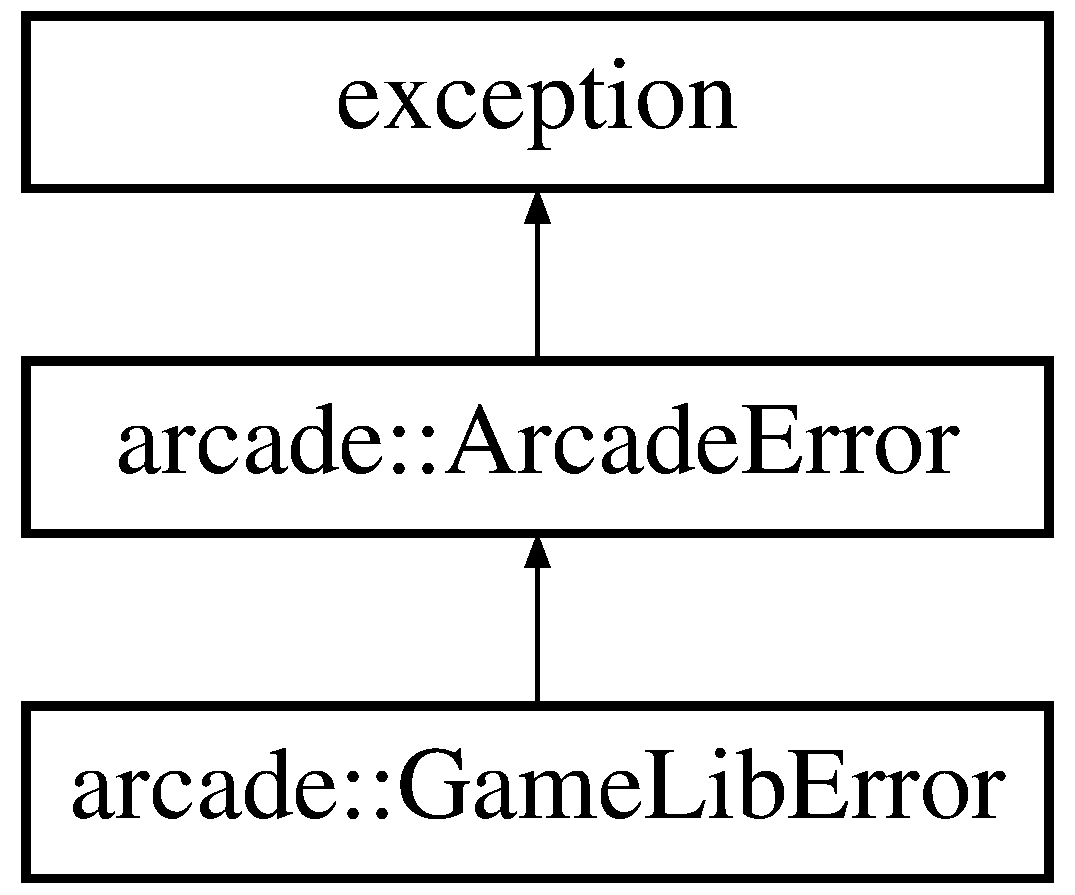
\includegraphics[height=3.000000cm]{classarcade_1_1_game_lib_error}
\end{center}
\end{figure}
\subsection*{Public Member Functions}
\begin{DoxyCompactItemize}
\item 
virtual \hyperlink{classarcade_1_1_game_lib_error_a38ca420e0e8f68b129af7121809d15a1}{$\sim$\+Game\+Lib\+Error} ()  throw ()
\item 
\hyperlink{classarcade_1_1_game_lib_error_ae409cbfd8f358f41a45eac59a1843b8b}{Game\+Lib\+Error} (const std\+::string \&msg)  throw ()
\end{DoxyCompactItemize}


\subsection{Constructor \& Destructor Documentation}
\mbox{\Hypertarget{classarcade_1_1_game_lib_error_a38ca420e0e8f68b129af7121809d15a1}\label{classarcade_1_1_game_lib_error_a38ca420e0e8f68b129af7121809d15a1}} 
\index{arcade\+::\+Game\+Lib\+Error@{arcade\+::\+Game\+Lib\+Error}!````~Game\+Lib\+Error@{$\sim$\+Game\+Lib\+Error}}
\index{````~Game\+Lib\+Error@{$\sim$\+Game\+Lib\+Error}!arcade\+::\+Game\+Lib\+Error@{arcade\+::\+Game\+Lib\+Error}}
\subsubsection{\texorpdfstring{$\sim$\+Game\+Lib\+Error()}{~GameLibError()}}
{\footnotesize\ttfamily arcade\+::\+Game\+Lib\+Error\+::$\sim$\+Game\+Lib\+Error (\begin{DoxyParamCaption}{ }\end{DoxyParamCaption}) throw  ) \hspace{0.3cm}{\ttfamily [virtual]}}

\mbox{\Hypertarget{classarcade_1_1_game_lib_error_ae409cbfd8f358f41a45eac59a1843b8b}\label{classarcade_1_1_game_lib_error_ae409cbfd8f358f41a45eac59a1843b8b}} 
\index{arcade\+::\+Game\+Lib\+Error@{arcade\+::\+Game\+Lib\+Error}!Game\+Lib\+Error@{Game\+Lib\+Error}}
\index{Game\+Lib\+Error@{Game\+Lib\+Error}!arcade\+::\+Game\+Lib\+Error@{arcade\+::\+Game\+Lib\+Error}}
\subsubsection{\texorpdfstring{Game\+Lib\+Error()}{GameLibError()}}
{\footnotesize\ttfamily arcade\+::\+Game\+Lib\+Error\+::\+Game\+Lib\+Error (\begin{DoxyParamCaption}\item[{const std\+::string \&}]{msg }\end{DoxyParamCaption}) throw  ) }



The documentation for this class was generated from the following files\+:\begin{DoxyCompactItemize}
\item 
include/\hyperlink{_exception_8hpp}{Exception.\+hpp}\item 
srcs/\hyperlink{_exception_8cpp}{Exception.\+cpp}\end{DoxyCompactItemize}

\hypertarget{structarcade_1_1_get_map}{}\section{arcade\+:\+:Get\+Map Struct Reference}
\label{structarcade_1_1_get_map}\index{arcade\+::\+Get\+Map@{arcade\+::\+Get\+Map}}


The format is width, height, and width $\ast$ height $\ast$ sizeof(\+Tile\+Type) quantity of Tile\+Type.  




{\ttfamily \#include $<$Protocol.\+hpp$>$}

\subsection*{Public Attributes}
\begin{DoxyCompactItemize}
\item 
\hyperlink{namespacearcade_a23d58aed7310b22b59e2b8f8ff8a5ffd}{Command\+Type} \hyperlink{structarcade_1_1_get_map_a1ea6878b06f00a3d2316dcd974bda8bf}{type}
\item 
uint16\+\_\+t \hyperlink{structarcade_1_1_get_map_a5d7616bd7955157ccdd663c1e0c9efe3}{width}
\item 
uint16\+\_\+t \hyperlink{structarcade_1_1_get_map_ae83569f92aa2a5cc6f50355162c62eb3}{height}
\item 
\hyperlink{namespacearcade_a61ba576694ea309cdf2b4b66902408ca}{Tile\+Type} \hyperlink{structarcade_1_1_get_map_acc3378cf49857df170f302ed959d0dea}{tile} \mbox{[}0\mbox{]}
\end{DoxyCompactItemize}


\subsection{Detailed Description}
The format is width, height, and width $\ast$ height $\ast$ sizeof(\+Tile\+Type) quantity of Tile\+Type. 

\subsection{Member Data Documentation}
\mbox{\Hypertarget{structarcade_1_1_get_map_ae83569f92aa2a5cc6f50355162c62eb3}\label{structarcade_1_1_get_map_ae83569f92aa2a5cc6f50355162c62eb3}} 
\index{arcade\+::\+Get\+Map@{arcade\+::\+Get\+Map}!height@{height}}
\index{height@{height}!arcade\+::\+Get\+Map@{arcade\+::\+Get\+Map}}
\subsubsection{\texorpdfstring{height}{height}}
{\footnotesize\ttfamily uint16\+\_\+t arcade\+::\+Get\+Map\+::height}

\mbox{\Hypertarget{structarcade_1_1_get_map_acc3378cf49857df170f302ed959d0dea}\label{structarcade_1_1_get_map_acc3378cf49857df170f302ed959d0dea}} 
\index{arcade\+::\+Get\+Map@{arcade\+::\+Get\+Map}!tile@{tile}}
\index{tile@{tile}!arcade\+::\+Get\+Map@{arcade\+::\+Get\+Map}}
\subsubsection{\texorpdfstring{tile}{tile}}
{\footnotesize\ttfamily \hyperlink{namespacearcade_a61ba576694ea309cdf2b4b66902408ca}{Tile\+Type} arcade\+::\+Get\+Map\+::tile\mbox{[}0\mbox{]}}

\mbox{\Hypertarget{structarcade_1_1_get_map_a1ea6878b06f00a3d2316dcd974bda8bf}\label{structarcade_1_1_get_map_a1ea6878b06f00a3d2316dcd974bda8bf}} 
\index{arcade\+::\+Get\+Map@{arcade\+::\+Get\+Map}!type@{type}}
\index{type@{type}!arcade\+::\+Get\+Map@{arcade\+::\+Get\+Map}}
\subsubsection{\texorpdfstring{type}{type}}
{\footnotesize\ttfamily \hyperlink{namespacearcade_a23d58aed7310b22b59e2b8f8ff8a5ffd}{Command\+Type} arcade\+::\+Get\+Map\+::type}

\mbox{\Hypertarget{structarcade_1_1_get_map_a5d7616bd7955157ccdd663c1e0c9efe3}\label{structarcade_1_1_get_map_a5d7616bd7955157ccdd663c1e0c9efe3}} 
\index{arcade\+::\+Get\+Map@{arcade\+::\+Get\+Map}!width@{width}}
\index{width@{width}!arcade\+::\+Get\+Map@{arcade\+::\+Get\+Map}}
\subsubsection{\texorpdfstring{width}{width}}
{\footnotesize\ttfamily uint16\+\_\+t arcade\+::\+Get\+Map\+::width}



The documentation for this struct was generated from the following file\+:\begin{DoxyCompactItemize}
\item 
include/\hyperlink{include_2_protocol_8hpp}{Protocol.\+hpp}\end{DoxyCompactItemize}

\hypertarget{classarcade_1_1_gfx_lapin}{}\section{arcade\+:\+:Gfx\+Lapin Class Reference}
\label{classarcade_1_1_gfx_lapin}\index{arcade\+::\+Gfx\+Lapin@{arcade\+::\+Gfx\+Lapin}}


{\ttfamily \#include $<$Gfx\+Lapin.\+hpp$>$}

Inheritance diagram for arcade\+:\+:Gfx\+Lapin\+:\begin{figure}[H]
\begin{center}
\leavevmode
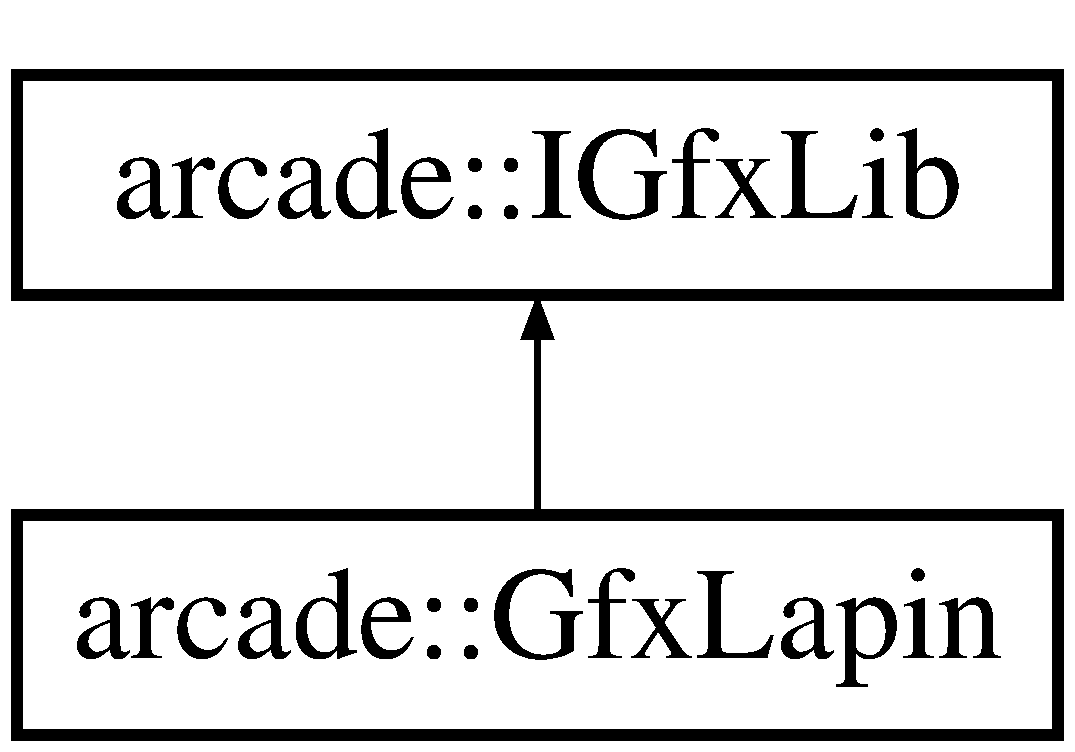
\includegraphics[height=2.000000cm]{classarcade_1_1_gfx_lapin}
\end{center}
\end{figure}
\subsection*{Classes}
\begin{DoxyCompactItemize}
\item 
struct \hyperlink{structarcade_1_1_gfx_lapin_1_1bunny__window}{bunny\+\_\+window}
\end{DoxyCompactItemize}
\subsection*{Public Member Functions}
\begin{DoxyCompactItemize}
\item 
virtual \hyperlink{classarcade_1_1_gfx_lapin_a87275ed29f549db04dc3888ace3fc73e}{$\sim$\+Gfx\+Lapin} ()
\item 
\hyperlink{classarcade_1_1_gfx_lapin_a23c348cc21e8b935c1922bc68b1950fb}{Gfx\+Lapin} ()
\item 
bool \hyperlink{classarcade_1_1_gfx_lapin_a80f4cae576f05ddc8ab94d5a348226c5}{poll\+Event} (\hyperlink{structarcade_1_1_event}{Event} \&e) override
\begin{DoxyCompactList}\small\item\em Function to poll events from the graphic lib. \end{DoxyCompactList}\item 
bool \hyperlink{classarcade_1_1_gfx_lapin_ae84337d3ae5e24a61f160d3ac99d4e10}{does\+Support\+Sound} () const override
\begin{DoxyCompactList}\small\item\em Ask if the library support sound. \end{DoxyCompactList}\item 
void \hyperlink{classarcade_1_1_gfx_lapin_a54039353c2da52bb45b233d4b8839551}{load\+Sounds} (std\+::vector$<$ std\+::pair$<$ std\+::string, \hyperlink{namespacearcade_a3bb4743a2eea59f3927e404e6549cae5}{Sound\+Type} $>$ $>$ const \&sounds) override
\begin{DoxyCompactList}\small\item\em Ask the lib to remove and load new sounds. \end{DoxyCompactList}\item 
void \hyperlink{classarcade_1_1_gfx_lapin_ad0f1a1014b88cf7f51ea85ab99e0c87b}{sound\+Control} (const \hyperlink{structarcade_1_1_sound}{Sound} \&sound) override
\begin{DoxyCompactList}\small\item\em Ask the lib to play a sound. \end{DoxyCompactList}\item 
void \hyperlink{classarcade_1_1_gfx_lapin_a164a694063507041dbd78415898d5157}{load\+Sprites} (std\+::vector$<$ std\+::unique\+\_\+ptr$<$ \hyperlink{classarcade_1_1_i_sprite}{I\+Sprite} $>$$>$ \&\&sprites) override
\begin{DoxyCompactList}\small\item\em Load sprites in the lib from the paths given by the game. \end{DoxyCompactList}\item 
void \hyperlink{classarcade_1_1_gfx_lapin_a06f4eb48bd1ea7749d81870211115a46}{update\+Map} (\hyperlink{classarcade_1_1_i_map}{I\+Map} const \&map) override
\begin{DoxyCompactList}\small\item\em Update the map displayed. \end{DoxyCompactList}\item 
void \hyperlink{classarcade_1_1_gfx_lapin_a6b226d0278ba5d43e956eb28557124ef}{update\+G\+UI} (\hyperlink{classarcade_1_1_i_g_u_i}{I\+G\+UI} \&gui) override
\begin{DoxyCompactList}\small\item\em Update the \hyperlink{classarcade_1_1_g_u_i}{G\+UI} displayed. \end{DoxyCompactList}\item 
void \hyperlink{classarcade_1_1_gfx_lapin_ac7c96886eb54a7d2f18e528e8f0c7ba1}{display} () override
\begin{DoxyCompactList}\small\item\em Display the map and \hyperlink{classarcade_1_1_g_u_i}{G\+UI}. \end{DoxyCompactList}\item 
void \hyperlink{classarcade_1_1_gfx_lapin_a42dd719cbf1cd88c3abf70d16f02fd92}{clear} () override
\begin{DoxyCompactList}\small\item\em Ask the lib to clear the screen. \end{DoxyCompactList}\end{DoxyCompactItemize}


\subsection{Constructor \& Destructor Documentation}
\mbox{\Hypertarget{classarcade_1_1_gfx_lapin_a87275ed29f549db04dc3888ace3fc73e}\label{classarcade_1_1_gfx_lapin_a87275ed29f549db04dc3888ace3fc73e}} 
\index{arcade\+::\+Gfx\+Lapin@{arcade\+::\+Gfx\+Lapin}!````~Gfx\+Lapin@{$\sim$\+Gfx\+Lapin}}
\index{````~Gfx\+Lapin@{$\sim$\+Gfx\+Lapin}!arcade\+::\+Gfx\+Lapin@{arcade\+::\+Gfx\+Lapin}}
\subsubsection{\texorpdfstring{$\sim$\+Gfx\+Lapin()}{~GfxLapin()}}
{\footnotesize\ttfamily arcade\+::\+Gfx\+Lapin\+::$\sim$\+Gfx\+Lapin (\begin{DoxyParamCaption}{ }\end{DoxyParamCaption})\hspace{0.3cm}{\ttfamily [virtual]}}

\mbox{\Hypertarget{classarcade_1_1_gfx_lapin_a23c348cc21e8b935c1922bc68b1950fb}\label{classarcade_1_1_gfx_lapin_a23c348cc21e8b935c1922bc68b1950fb}} 
\index{arcade\+::\+Gfx\+Lapin@{arcade\+::\+Gfx\+Lapin}!Gfx\+Lapin@{Gfx\+Lapin}}
\index{Gfx\+Lapin@{Gfx\+Lapin}!arcade\+::\+Gfx\+Lapin@{arcade\+::\+Gfx\+Lapin}}
\subsubsection{\texorpdfstring{Gfx\+Lapin()}{GfxLapin()}}
{\footnotesize\ttfamily arcade\+::\+Gfx\+Lapin\+::\+Gfx\+Lapin (\begin{DoxyParamCaption}{ }\end{DoxyParamCaption})}

A key

B key

C key

D key

E key

F key

G key

H key

I key

J key

K key

L key

M key

N key

O key

P key

Q key

R key

S key

T key

U key

V key

X key

Y key

Z key

0 key

1 key

2 key

3 key

4 key

5 key

6 key

7 key

8 key

9 key

Left arrow key

Right arrow key

Up arrow key

Down arrow key

Space key

Enter/\+Carriage return key

Backspace key

Left Control key

Right Control key

Left Alt key

Right Alt key

Left Shift key

Right Shift key

Tabulation key

Escape key

Page up key

Page down

Home key

End key

Function key 1 (F1)

Function key 2 (F2)

Function key 3 (F3)

Function key 4 (F4)

Function key 5 (F5)

Function key 6 (F6)

Function key 7 (F7)

Function key 8 (F8)

Function key 9 (F9)

Function key 10 (F10)

Function key 11 (F11)

Function key 12 (F12)

Comma key (,)

Dot (period) key (.)

Slash key (/)

Semicolon key (;)

Simple quote key (\textquotesingle{})

Left bracket key (\mbox{[})

Right bracker key (\mbox{]})

Backslash key ()

Asterisk key ($\ast$)

Minus symbol key (-\/)

Plus symbol key (+) 

\subsection{Member Function Documentation}
\mbox{\Hypertarget{classarcade_1_1_gfx_lapin_a42dd719cbf1cd88c3abf70d16f02fd92}\label{classarcade_1_1_gfx_lapin_a42dd719cbf1cd88c3abf70d16f02fd92}} 
\index{arcade\+::\+Gfx\+Lapin@{arcade\+::\+Gfx\+Lapin}!clear@{clear}}
\index{clear@{clear}!arcade\+::\+Gfx\+Lapin@{arcade\+::\+Gfx\+Lapin}}
\subsubsection{\texorpdfstring{clear()}{clear()}}
{\footnotesize\ttfamily void arcade\+::\+Gfx\+Lapin\+::clear (\begin{DoxyParamCaption}{ }\end{DoxyParamCaption})\hspace{0.3cm}{\ttfamily [override]}, {\ttfamily [virtual]}}



Ask the lib to clear the screen. 



Implements \hyperlink{classarcade_1_1_i_gfx_lib_a4116b3d4f503c4a795539b584f77a73d}{arcade\+::\+I\+Gfx\+Lib}.

\mbox{\Hypertarget{classarcade_1_1_gfx_lapin_ac7c96886eb54a7d2f18e528e8f0c7ba1}\label{classarcade_1_1_gfx_lapin_ac7c96886eb54a7d2f18e528e8f0c7ba1}} 
\index{arcade\+::\+Gfx\+Lapin@{arcade\+::\+Gfx\+Lapin}!display@{display}}
\index{display@{display}!arcade\+::\+Gfx\+Lapin@{arcade\+::\+Gfx\+Lapin}}
\subsubsection{\texorpdfstring{display()}{display()}}
{\footnotesize\ttfamily void arcade\+::\+Gfx\+Lapin\+::display (\begin{DoxyParamCaption}{ }\end{DoxyParamCaption})\hspace{0.3cm}{\ttfamily [override]}, {\ttfamily [virtual]}}



Display the map and \hyperlink{classarcade_1_1_g_u_i}{G\+UI}. 



Implements \hyperlink{classarcade_1_1_i_gfx_lib_a7f280525c718a44c1e05cfe0ba5304c3}{arcade\+::\+I\+Gfx\+Lib}.

\mbox{\Hypertarget{classarcade_1_1_gfx_lapin_ae84337d3ae5e24a61f160d3ac99d4e10}\label{classarcade_1_1_gfx_lapin_ae84337d3ae5e24a61f160d3ac99d4e10}} 
\index{arcade\+::\+Gfx\+Lapin@{arcade\+::\+Gfx\+Lapin}!does\+Support\+Sound@{does\+Support\+Sound}}
\index{does\+Support\+Sound@{does\+Support\+Sound}!arcade\+::\+Gfx\+Lapin@{arcade\+::\+Gfx\+Lapin}}
\subsubsection{\texorpdfstring{does\+Support\+Sound()}{doesSupportSound()}}
{\footnotesize\ttfamily bool arcade\+::\+Gfx\+Lapin\+::does\+Support\+Sound (\begin{DoxyParamCaption}{ }\end{DoxyParamCaption}) const\hspace{0.3cm}{\ttfamily [override]}, {\ttfamily [virtual]}}



Ask if the library support sound. 



Implements \hyperlink{classarcade_1_1_i_gfx_lib_a68cfbc987dfecca5b1405e36e00157b2}{arcade\+::\+I\+Gfx\+Lib}.

\mbox{\Hypertarget{classarcade_1_1_gfx_lapin_a54039353c2da52bb45b233d4b8839551}\label{classarcade_1_1_gfx_lapin_a54039353c2da52bb45b233d4b8839551}} 
\index{arcade\+::\+Gfx\+Lapin@{arcade\+::\+Gfx\+Lapin}!load\+Sounds@{load\+Sounds}}
\index{load\+Sounds@{load\+Sounds}!arcade\+::\+Gfx\+Lapin@{arcade\+::\+Gfx\+Lapin}}
\subsubsection{\texorpdfstring{load\+Sounds()}{loadSounds()}}
{\footnotesize\ttfamily void arcade\+::\+Gfx\+Lapin\+::load\+Sounds (\begin{DoxyParamCaption}\item[{std\+::vector$<$ std\+::pair$<$ std\+::string, \hyperlink{namespacearcade_a3bb4743a2eea59f3927e404e6549cae5}{Sound\+Type} $>$ $>$ const \&}]{sounds }\end{DoxyParamCaption})\hspace{0.3cm}{\ttfamily [override]}, {\ttfamily [virtual]}}



Ask the lib to remove and load new sounds. 



Implements \hyperlink{classarcade_1_1_i_gfx_lib_a725faf0722d284d15eb389b0a1891a27}{arcade\+::\+I\+Gfx\+Lib}.

\mbox{\Hypertarget{classarcade_1_1_gfx_lapin_a164a694063507041dbd78415898d5157}\label{classarcade_1_1_gfx_lapin_a164a694063507041dbd78415898d5157}} 
\index{arcade\+::\+Gfx\+Lapin@{arcade\+::\+Gfx\+Lapin}!load\+Sprites@{load\+Sprites}}
\index{load\+Sprites@{load\+Sprites}!arcade\+::\+Gfx\+Lapin@{arcade\+::\+Gfx\+Lapin}}
\subsubsection{\texorpdfstring{load\+Sprites()}{loadSprites()}}
{\footnotesize\ttfamily void arcade\+::\+Gfx\+Lapin\+::load\+Sprites (\begin{DoxyParamCaption}\item[{std\+::vector$<$ std\+::unique\+\_\+ptr$<$ \hyperlink{classarcade_1_1_i_sprite}{I\+Sprite} $>$$>$ \&\&}]{sprites }\end{DoxyParamCaption})\hspace{0.3cm}{\ttfamily [override]}, {\ttfamily [virtual]}}



Load sprites in the lib from the paths given by the game. 


\begin{DoxyParams}{Parameters}
{\em sprites} & to pass the path of your sprites to give your lib the way to search your assets \\
\hline
\end{DoxyParams}


Implements \hyperlink{classarcade_1_1_i_gfx_lib_ad5b301c8ff56c428971a2a006514b709}{arcade\+::\+I\+Gfx\+Lib}.

\mbox{\Hypertarget{classarcade_1_1_gfx_lapin_a80f4cae576f05ddc8ab94d5a348226c5}\label{classarcade_1_1_gfx_lapin_a80f4cae576f05ddc8ab94d5a348226c5}} 
\index{arcade\+::\+Gfx\+Lapin@{arcade\+::\+Gfx\+Lapin}!poll\+Event@{poll\+Event}}
\index{poll\+Event@{poll\+Event}!arcade\+::\+Gfx\+Lapin@{arcade\+::\+Gfx\+Lapin}}
\subsubsection{\texorpdfstring{poll\+Event()}{pollEvent()}}
{\footnotesize\ttfamily bool arcade\+::\+Gfx\+Lapin\+::poll\+Event (\begin{DoxyParamCaption}\item[{\hyperlink{structarcade_1_1_event}{arcade\+::\+Event} \&}]{e }\end{DoxyParamCaption})\hspace{0.3cm}{\ttfamily [override]}, {\ttfamily [virtual]}}



Function to poll events from the graphic lib. 

If there is an event to poll, e is filled and true is returned. If not, false is returned. 

Implements \hyperlink{classarcade_1_1_i_gfx_lib_a82cdd82f168ca898ef81edf82ca6147a}{arcade\+::\+I\+Gfx\+Lib}.

\mbox{\Hypertarget{classarcade_1_1_gfx_lapin_ad0f1a1014b88cf7f51ea85ab99e0c87b}\label{classarcade_1_1_gfx_lapin_ad0f1a1014b88cf7f51ea85ab99e0c87b}} 
\index{arcade\+::\+Gfx\+Lapin@{arcade\+::\+Gfx\+Lapin}!sound\+Control@{sound\+Control}}
\index{sound\+Control@{sound\+Control}!arcade\+::\+Gfx\+Lapin@{arcade\+::\+Gfx\+Lapin}}
\subsubsection{\texorpdfstring{sound\+Control()}{soundControl()}}
{\footnotesize\ttfamily void arcade\+::\+Gfx\+Lapin\+::sound\+Control (\begin{DoxyParamCaption}\item[{const \hyperlink{structarcade_1_1_sound}{Sound} \&}]{sound }\end{DoxyParamCaption})\hspace{0.3cm}{\ttfamily [override]}, {\ttfamily [virtual]}}



Ask the lib to play a sound. 



Implements \hyperlink{classarcade_1_1_i_gfx_lib_a0b965ed555739ef366b27583799d794c}{arcade\+::\+I\+Gfx\+Lib}.

\mbox{\Hypertarget{classarcade_1_1_gfx_lapin_a6b226d0278ba5d43e956eb28557124ef}\label{classarcade_1_1_gfx_lapin_a6b226d0278ba5d43e956eb28557124ef}} 
\index{arcade\+::\+Gfx\+Lapin@{arcade\+::\+Gfx\+Lapin}!update\+G\+UI@{update\+G\+UI}}
\index{update\+G\+UI@{update\+G\+UI}!arcade\+::\+Gfx\+Lapin@{arcade\+::\+Gfx\+Lapin}}
\subsubsection{\texorpdfstring{update\+G\+U\+I()}{updateGUI()}}
{\footnotesize\ttfamily void arcade\+::\+Gfx\+Lapin\+::update\+G\+UI (\begin{DoxyParamCaption}\item[{\hyperlink{classarcade_1_1_i_g_u_i}{I\+G\+UI} \&}]{gui }\end{DoxyParamCaption})\hspace{0.3cm}{\ttfamily [override]}, {\ttfamily [virtual]}}



Update the \hyperlink{classarcade_1_1_g_u_i}{G\+UI} displayed. 



Implements \hyperlink{classarcade_1_1_i_gfx_lib_ae3f443cc341512433815e8bf2dee3e0d}{arcade\+::\+I\+Gfx\+Lib}.

\mbox{\Hypertarget{classarcade_1_1_gfx_lapin_a06f4eb48bd1ea7749d81870211115a46}\label{classarcade_1_1_gfx_lapin_a06f4eb48bd1ea7749d81870211115a46}} 
\index{arcade\+::\+Gfx\+Lapin@{arcade\+::\+Gfx\+Lapin}!update\+Map@{update\+Map}}
\index{update\+Map@{update\+Map}!arcade\+::\+Gfx\+Lapin@{arcade\+::\+Gfx\+Lapin}}
\subsubsection{\texorpdfstring{update\+Map()}{updateMap()}}
{\footnotesize\ttfamily void arcade\+::\+Gfx\+Lapin\+::update\+Map (\begin{DoxyParamCaption}\item[{\hyperlink{classarcade_1_1_i_map}{I\+Map} const \&}]{map }\end{DoxyParamCaption})\hspace{0.3cm}{\ttfamily [override]}, {\ttfamily [virtual]}}



Update the map displayed. 



Implements \hyperlink{classarcade_1_1_i_gfx_lib_addc883f69b75e6ec4927027aad94f5b5}{arcade\+::\+I\+Gfx\+Lib}.



The documentation for this class was generated from the following files\+:\begin{DoxyCompactItemize}
\item 
gfx\+Libs\+Srcs/lapin/include/\hyperlink{_gfx_lapin_8hpp}{Gfx\+Lapin.\+hpp}\item 
gfx\+Libs\+Srcs/lapin/src/\hyperlink{_gfx_lapin_8cpp}{Gfx\+Lapin.\+cpp}\item 
gfx\+Libs\+Srcs/lapin/src/\hyperlink{tektext_8cpp}{tektext.\+cpp}\end{DoxyCompactItemize}

\hypertarget{classarcade_1_1_gfx_lib_error}{}\section{arcade\+:\+:Gfx\+Lib\+Error Class Reference}
\label{classarcade_1_1_gfx_lib_error}\index{arcade\+::\+Gfx\+Lib\+Error@{arcade\+::\+Gfx\+Lib\+Error}}


{\ttfamily \#include $<$Exception.\+hpp$>$}

Inheritance diagram for arcade\+:\+:Gfx\+Lib\+Error\+:\begin{figure}[H]
\begin{center}
\leavevmode
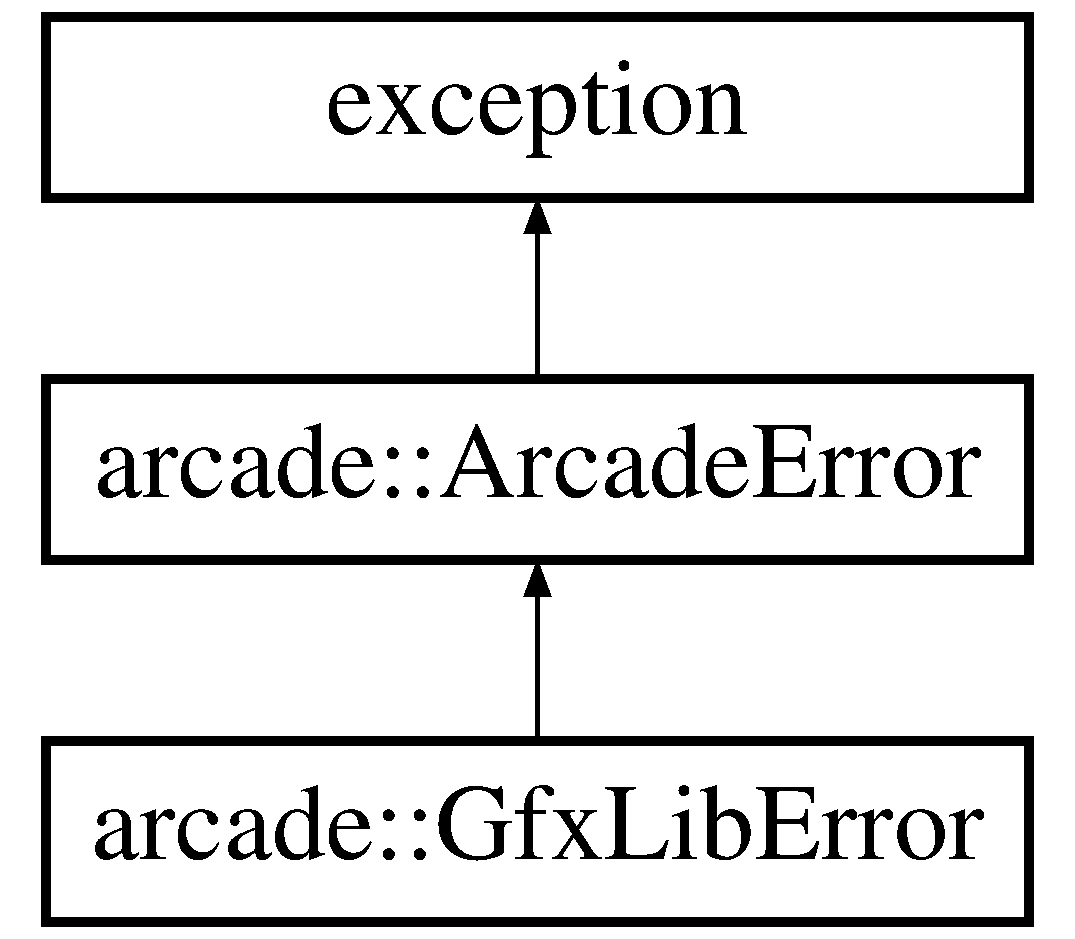
\includegraphics[height=3.000000cm]{classarcade_1_1_gfx_lib_error}
\end{center}
\end{figure}
\subsection*{Public Member Functions}
\begin{DoxyCompactItemize}
\item 
virtual \hyperlink{classarcade_1_1_gfx_lib_error_a8ca4f3f6dd5896c71838b770c4a95200}{$\sim$\+Gfx\+Lib\+Error} ()  throw ()
\item 
\hyperlink{classarcade_1_1_gfx_lib_error_a4a74810744427eecd13717581ae29cda}{Gfx\+Lib\+Error} (const std\+::string \&msg)  throw ()
\end{DoxyCompactItemize}


\subsection{Constructor \& Destructor Documentation}
\mbox{\Hypertarget{classarcade_1_1_gfx_lib_error_a8ca4f3f6dd5896c71838b770c4a95200}\label{classarcade_1_1_gfx_lib_error_a8ca4f3f6dd5896c71838b770c4a95200}} 
\index{arcade\+::\+Gfx\+Lib\+Error@{arcade\+::\+Gfx\+Lib\+Error}!````~Gfx\+Lib\+Error@{$\sim$\+Gfx\+Lib\+Error}}
\index{````~Gfx\+Lib\+Error@{$\sim$\+Gfx\+Lib\+Error}!arcade\+::\+Gfx\+Lib\+Error@{arcade\+::\+Gfx\+Lib\+Error}}
\subsubsection{\texorpdfstring{$\sim$\+Gfx\+Lib\+Error()}{~GfxLibError()}}
{\footnotesize\ttfamily arcade\+::\+Gfx\+Lib\+Error\+::$\sim$\+Gfx\+Lib\+Error (\begin{DoxyParamCaption}{ }\end{DoxyParamCaption}) throw  ) \hspace{0.3cm}{\ttfamily [virtual]}}

\mbox{\Hypertarget{classarcade_1_1_gfx_lib_error_a4a74810744427eecd13717581ae29cda}\label{classarcade_1_1_gfx_lib_error_a4a74810744427eecd13717581ae29cda}} 
\index{arcade\+::\+Gfx\+Lib\+Error@{arcade\+::\+Gfx\+Lib\+Error}!Gfx\+Lib\+Error@{Gfx\+Lib\+Error}}
\index{Gfx\+Lib\+Error@{Gfx\+Lib\+Error}!arcade\+::\+Gfx\+Lib\+Error@{arcade\+::\+Gfx\+Lib\+Error}}
\subsubsection{\texorpdfstring{Gfx\+Lib\+Error()}{GfxLibError()}}
{\footnotesize\ttfamily arcade\+::\+Gfx\+Lib\+Error\+::\+Gfx\+Lib\+Error (\begin{DoxyParamCaption}\item[{const std\+::string \&}]{msg }\end{DoxyParamCaption}) throw  ) }



The documentation for this class was generated from the following files\+:\begin{DoxyCompactItemize}
\item 
include/\hyperlink{_exception_8hpp}{Exception.\+hpp}\item 
srcs/\hyperlink{_exception_8cpp}{Exception.\+cpp}\end{DoxyCompactItemize}

\hypertarget{classarcade_1_1_gfx_ncurses}{}\section{arcade\+:\+:Gfx\+Ncurses Class Reference}
\label{classarcade_1_1_gfx_ncurses}\index{arcade\+::\+Gfx\+Ncurses@{arcade\+::\+Gfx\+Ncurses}}


{\ttfamily \#include $<$Gfx\+Ncurses.\+hpp$>$}

Inheritance diagram for arcade\+:\+:Gfx\+Ncurses\+:\begin{figure}[H]
\begin{center}
\leavevmode
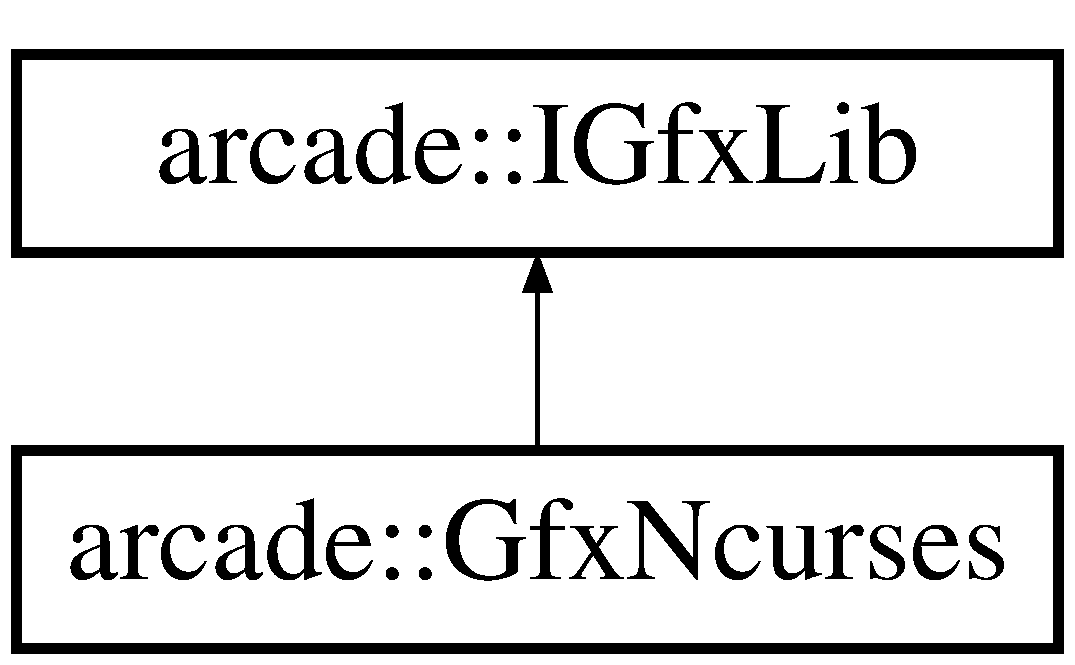
\includegraphics[height=2.000000cm]{classarcade_1_1_gfx_ncurses}
\end{center}
\end{figure}
\subsection*{Public Member Functions}
\begin{DoxyCompactItemize}
\item 
\hyperlink{classarcade_1_1_gfx_ncurses_a0408b1bf8ad9b35de30d82fe2c0512f2}{Gfx\+Ncurses} ()
\item 
\hyperlink{classarcade_1_1_gfx_ncurses_a462de36e41ccd26eba4e908ee3603a4b}{$\sim$\+Gfx\+Ncurses} ()
\item 
bool \hyperlink{classarcade_1_1_gfx_ncurses_aa16f7c823041b931025f750b4050318a}{poll\+Event} (\hyperlink{structarcade_1_1_event}{Event} \&e) override
\begin{DoxyCompactList}\small\item\em Function to poll events from the graphic lib. \end{DoxyCompactList}\item 
bool \hyperlink{classarcade_1_1_gfx_ncurses_ab100f60173ccd55f19c30627ace55101}{does\+Support\+Sound} () const override
\begin{DoxyCompactList}\small\item\em Ask if the library support sound. \end{DoxyCompactList}\item 
void \hyperlink{classarcade_1_1_gfx_ncurses_a450bb0bdb3a31f8733cc71cb39ddfb16}{load\+Sounds} (std\+::vector$<$ std\+::pair$<$ std\+::string, \hyperlink{namespacearcade_a3bb4743a2eea59f3927e404e6549cae5}{Sound\+Type} $>$ $>$ const \&sounds) override
\begin{DoxyCompactList}\small\item\em Ask the lib to remove and load new sounds. \end{DoxyCompactList}\item 
void \hyperlink{classarcade_1_1_gfx_ncurses_a5eabfc85f5ae13bf0592dd21add9f301}{sound\+Control} (const \hyperlink{structarcade_1_1_sound}{Sound} \&sound) override
\begin{DoxyCompactList}\small\item\em Ask the lib to play a sound. \end{DoxyCompactList}\item 
void \hyperlink{classarcade_1_1_gfx_ncurses_a6a412ec8047964035f0d75e64fd8dc44}{load\+Sprites} (std\+::vector$<$ std\+::unique\+\_\+ptr$<$ \hyperlink{classarcade_1_1_i_sprite}{I\+Sprite} $>$$>$ \&\&sprites) override
\begin{DoxyCompactList}\small\item\em Load sprites in the lib from the paths given by the game. \end{DoxyCompactList}\item 
void \hyperlink{classarcade_1_1_gfx_ncurses_a4e02400d983845ebe37f374f3dd82793}{update\+Map} (\hyperlink{classarcade_1_1_i_map}{I\+Map} const \&map) override
\begin{DoxyCompactList}\small\item\em Update the map displayed. \end{DoxyCompactList}\item 
void \hyperlink{classarcade_1_1_gfx_ncurses_a00469b26c23ff57efdbb2f99dedbbb11}{update\+G\+UI} (\hyperlink{classarcade_1_1_i_g_u_i}{I\+G\+UI} \&gui) override
\begin{DoxyCompactList}\small\item\em Update the \hyperlink{classarcade_1_1_g_u_i}{G\+UI} displayed. \end{DoxyCompactList}\item 
void \hyperlink{classarcade_1_1_gfx_ncurses_aa119cdff68869bcd3829bb9fa9eaa373}{display} () override
\begin{DoxyCompactList}\small\item\em Display the map and \hyperlink{classarcade_1_1_g_u_i}{G\+UI}. \end{DoxyCompactList}\item 
void \hyperlink{classarcade_1_1_gfx_ncurses_aaf443541674ace2e915e393156adf232}{clear} () override
\begin{DoxyCompactList}\small\item\em Ask the lib to clear the screen. \end{DoxyCompactList}\end{DoxyCompactItemize}


\subsection{Constructor \& Destructor Documentation}
\mbox{\Hypertarget{classarcade_1_1_gfx_ncurses_a0408b1bf8ad9b35de30d82fe2c0512f2}\label{classarcade_1_1_gfx_ncurses_a0408b1bf8ad9b35de30d82fe2c0512f2}} 
\index{arcade\+::\+Gfx\+Ncurses@{arcade\+::\+Gfx\+Ncurses}!Gfx\+Ncurses@{Gfx\+Ncurses}}
\index{Gfx\+Ncurses@{Gfx\+Ncurses}!arcade\+::\+Gfx\+Ncurses@{arcade\+::\+Gfx\+Ncurses}}
\subsubsection{\texorpdfstring{Gfx\+Ncurses()}{GfxNcurses()}}
{\footnotesize\ttfamily arcade\+::\+Gfx\+Ncurses\+::\+Gfx\+Ncurses (\begin{DoxyParamCaption}{ }\end{DoxyParamCaption})}

\mbox{\Hypertarget{classarcade_1_1_gfx_ncurses_a462de36e41ccd26eba4e908ee3603a4b}\label{classarcade_1_1_gfx_ncurses_a462de36e41ccd26eba4e908ee3603a4b}} 
\index{arcade\+::\+Gfx\+Ncurses@{arcade\+::\+Gfx\+Ncurses}!````~Gfx\+Ncurses@{$\sim$\+Gfx\+Ncurses}}
\index{````~Gfx\+Ncurses@{$\sim$\+Gfx\+Ncurses}!arcade\+::\+Gfx\+Ncurses@{arcade\+::\+Gfx\+Ncurses}}
\subsubsection{\texorpdfstring{$\sim$\+Gfx\+Ncurses()}{~GfxNcurses()}}
{\footnotesize\ttfamily arcade\+::\+Gfx\+Ncurses\+::$\sim$\+Gfx\+Ncurses (\begin{DoxyParamCaption}{ }\end{DoxyParamCaption})}



\subsection{Member Function Documentation}
\mbox{\Hypertarget{classarcade_1_1_gfx_ncurses_aaf443541674ace2e915e393156adf232}\label{classarcade_1_1_gfx_ncurses_aaf443541674ace2e915e393156adf232}} 
\index{arcade\+::\+Gfx\+Ncurses@{arcade\+::\+Gfx\+Ncurses}!clear@{clear}}
\index{clear@{clear}!arcade\+::\+Gfx\+Ncurses@{arcade\+::\+Gfx\+Ncurses}}
\subsubsection{\texorpdfstring{clear()}{clear()}}
{\footnotesize\ttfamily void arcade\+::\+Gfx\+Ncurses\+::clear (\begin{DoxyParamCaption}{ }\end{DoxyParamCaption})\hspace{0.3cm}{\ttfamily [override]}, {\ttfamily [virtual]}}



Ask the lib to clear the screen. 



Implements \hyperlink{classarcade_1_1_i_gfx_lib_a4116b3d4f503c4a795539b584f77a73d}{arcade\+::\+I\+Gfx\+Lib}.

\mbox{\Hypertarget{classarcade_1_1_gfx_ncurses_aa119cdff68869bcd3829bb9fa9eaa373}\label{classarcade_1_1_gfx_ncurses_aa119cdff68869bcd3829bb9fa9eaa373}} 
\index{arcade\+::\+Gfx\+Ncurses@{arcade\+::\+Gfx\+Ncurses}!display@{display}}
\index{display@{display}!arcade\+::\+Gfx\+Ncurses@{arcade\+::\+Gfx\+Ncurses}}
\subsubsection{\texorpdfstring{display()}{display()}}
{\footnotesize\ttfamily void arcade\+::\+Gfx\+Ncurses\+::display (\begin{DoxyParamCaption}{ }\end{DoxyParamCaption})\hspace{0.3cm}{\ttfamily [override]}, {\ttfamily [virtual]}}



Display the map and \hyperlink{classarcade_1_1_g_u_i}{G\+UI}. 



Implements \hyperlink{classarcade_1_1_i_gfx_lib_a7f280525c718a44c1e05cfe0ba5304c3}{arcade\+::\+I\+Gfx\+Lib}.

\mbox{\Hypertarget{classarcade_1_1_gfx_ncurses_ab100f60173ccd55f19c30627ace55101}\label{classarcade_1_1_gfx_ncurses_ab100f60173ccd55f19c30627ace55101}} 
\index{arcade\+::\+Gfx\+Ncurses@{arcade\+::\+Gfx\+Ncurses}!does\+Support\+Sound@{does\+Support\+Sound}}
\index{does\+Support\+Sound@{does\+Support\+Sound}!arcade\+::\+Gfx\+Ncurses@{arcade\+::\+Gfx\+Ncurses}}
\subsubsection{\texorpdfstring{does\+Support\+Sound()}{doesSupportSound()}}
{\footnotesize\ttfamily bool arcade\+::\+Gfx\+Ncurses\+::does\+Support\+Sound (\begin{DoxyParamCaption}{ }\end{DoxyParamCaption}) const\hspace{0.3cm}{\ttfamily [override]}, {\ttfamily [virtual]}}



Ask if the library support sound. 



Implements \hyperlink{classarcade_1_1_i_gfx_lib_a68cfbc987dfecca5b1405e36e00157b2}{arcade\+::\+I\+Gfx\+Lib}.

\mbox{\Hypertarget{classarcade_1_1_gfx_ncurses_a450bb0bdb3a31f8733cc71cb39ddfb16}\label{classarcade_1_1_gfx_ncurses_a450bb0bdb3a31f8733cc71cb39ddfb16}} 
\index{arcade\+::\+Gfx\+Ncurses@{arcade\+::\+Gfx\+Ncurses}!load\+Sounds@{load\+Sounds}}
\index{load\+Sounds@{load\+Sounds}!arcade\+::\+Gfx\+Ncurses@{arcade\+::\+Gfx\+Ncurses}}
\subsubsection{\texorpdfstring{load\+Sounds()}{loadSounds()}}
{\footnotesize\ttfamily void arcade\+::\+Gfx\+Ncurses\+::load\+Sounds (\begin{DoxyParamCaption}\item[{std\+::vector$<$ std\+::pair$<$ std\+::string, \hyperlink{namespacearcade_a3bb4743a2eea59f3927e404e6549cae5}{Sound\+Type} $>$ $>$ const \&}]{sounds }\end{DoxyParamCaption})\hspace{0.3cm}{\ttfamily [override]}, {\ttfamily [virtual]}}



Ask the lib to remove and load new sounds. 



Implements \hyperlink{classarcade_1_1_i_gfx_lib_a725faf0722d284d15eb389b0a1891a27}{arcade\+::\+I\+Gfx\+Lib}.

\mbox{\Hypertarget{classarcade_1_1_gfx_ncurses_a6a412ec8047964035f0d75e64fd8dc44}\label{classarcade_1_1_gfx_ncurses_a6a412ec8047964035f0d75e64fd8dc44}} 
\index{arcade\+::\+Gfx\+Ncurses@{arcade\+::\+Gfx\+Ncurses}!load\+Sprites@{load\+Sprites}}
\index{load\+Sprites@{load\+Sprites}!arcade\+::\+Gfx\+Ncurses@{arcade\+::\+Gfx\+Ncurses}}
\subsubsection{\texorpdfstring{load\+Sprites()}{loadSprites()}}
{\footnotesize\ttfamily void arcade\+::\+Gfx\+Ncurses\+::load\+Sprites (\begin{DoxyParamCaption}\item[{std\+::vector$<$ std\+::unique\+\_\+ptr$<$ \hyperlink{classarcade_1_1_i_sprite}{I\+Sprite} $>$$>$ \&\&}]{sprites }\end{DoxyParamCaption})\hspace{0.3cm}{\ttfamily [override]}, {\ttfamily [virtual]}}



Load sprites in the lib from the paths given by the game. 


\begin{DoxyParams}{Parameters}
{\em sprites} & to pass the path of your sprites to give your lib the way to search your assets \\
\hline
\end{DoxyParams}


Implements \hyperlink{classarcade_1_1_i_gfx_lib_ad5b301c8ff56c428971a2a006514b709}{arcade\+::\+I\+Gfx\+Lib}.

\mbox{\Hypertarget{classarcade_1_1_gfx_ncurses_aa16f7c823041b931025f750b4050318a}\label{classarcade_1_1_gfx_ncurses_aa16f7c823041b931025f750b4050318a}} 
\index{arcade\+::\+Gfx\+Ncurses@{arcade\+::\+Gfx\+Ncurses}!poll\+Event@{poll\+Event}}
\index{poll\+Event@{poll\+Event}!arcade\+::\+Gfx\+Ncurses@{arcade\+::\+Gfx\+Ncurses}}
\subsubsection{\texorpdfstring{poll\+Event()}{pollEvent()}}
{\footnotesize\ttfamily bool arcade\+::\+Gfx\+Ncurses\+::poll\+Event (\begin{DoxyParamCaption}\item[{\hyperlink{structarcade_1_1_event}{arcade\+::\+Event} \&}]{e }\end{DoxyParamCaption})\hspace{0.3cm}{\ttfamily [override]}, {\ttfamily [virtual]}}



Function to poll events from the graphic lib. 

If there is an event to poll, e is filled and true is returned. If not, false is returned. 

Implements \hyperlink{classarcade_1_1_i_gfx_lib_a82cdd82f168ca898ef81edf82ca6147a}{arcade\+::\+I\+Gfx\+Lib}.

\mbox{\Hypertarget{classarcade_1_1_gfx_ncurses_a5eabfc85f5ae13bf0592dd21add9f301}\label{classarcade_1_1_gfx_ncurses_a5eabfc85f5ae13bf0592dd21add9f301}} 
\index{arcade\+::\+Gfx\+Ncurses@{arcade\+::\+Gfx\+Ncurses}!sound\+Control@{sound\+Control}}
\index{sound\+Control@{sound\+Control}!arcade\+::\+Gfx\+Ncurses@{arcade\+::\+Gfx\+Ncurses}}
\subsubsection{\texorpdfstring{sound\+Control()}{soundControl()}}
{\footnotesize\ttfamily void arcade\+::\+Gfx\+Ncurses\+::sound\+Control (\begin{DoxyParamCaption}\item[{const \hyperlink{structarcade_1_1_sound}{Sound} \&}]{sound }\end{DoxyParamCaption})\hspace{0.3cm}{\ttfamily [override]}, {\ttfamily [virtual]}}



Ask the lib to play a sound. 



Implements \hyperlink{classarcade_1_1_i_gfx_lib_a0b965ed555739ef366b27583799d794c}{arcade\+::\+I\+Gfx\+Lib}.

\mbox{\Hypertarget{classarcade_1_1_gfx_ncurses_a00469b26c23ff57efdbb2f99dedbbb11}\label{classarcade_1_1_gfx_ncurses_a00469b26c23ff57efdbb2f99dedbbb11}} 
\index{arcade\+::\+Gfx\+Ncurses@{arcade\+::\+Gfx\+Ncurses}!update\+G\+UI@{update\+G\+UI}}
\index{update\+G\+UI@{update\+G\+UI}!arcade\+::\+Gfx\+Ncurses@{arcade\+::\+Gfx\+Ncurses}}
\subsubsection{\texorpdfstring{update\+G\+U\+I()}{updateGUI()}}
{\footnotesize\ttfamily void arcade\+::\+Gfx\+Ncurses\+::update\+G\+UI (\begin{DoxyParamCaption}\item[{\hyperlink{classarcade_1_1_i_g_u_i}{I\+G\+UI} \&}]{gui }\end{DoxyParamCaption})\hspace{0.3cm}{\ttfamily [override]}, {\ttfamily [virtual]}}



Update the \hyperlink{classarcade_1_1_g_u_i}{G\+UI} displayed. 



Implements \hyperlink{classarcade_1_1_i_gfx_lib_ae3f443cc341512433815e8bf2dee3e0d}{arcade\+::\+I\+Gfx\+Lib}.

\mbox{\Hypertarget{classarcade_1_1_gfx_ncurses_a4e02400d983845ebe37f374f3dd82793}\label{classarcade_1_1_gfx_ncurses_a4e02400d983845ebe37f374f3dd82793}} 
\index{arcade\+::\+Gfx\+Ncurses@{arcade\+::\+Gfx\+Ncurses}!update\+Map@{update\+Map}}
\index{update\+Map@{update\+Map}!arcade\+::\+Gfx\+Ncurses@{arcade\+::\+Gfx\+Ncurses}}
\subsubsection{\texorpdfstring{update\+Map()}{updateMap()}}
{\footnotesize\ttfamily void arcade\+::\+Gfx\+Ncurses\+::update\+Map (\begin{DoxyParamCaption}\item[{\hyperlink{classarcade_1_1_i_map}{I\+Map} const \&}]{map }\end{DoxyParamCaption})\hspace{0.3cm}{\ttfamily [override]}, {\ttfamily [virtual]}}



Update the map displayed. 



Implements \hyperlink{classarcade_1_1_i_gfx_lib_addc883f69b75e6ec4927027aad94f5b5}{arcade\+::\+I\+Gfx\+Lib}.



The documentation for this class was generated from the following files\+:\begin{DoxyCompactItemize}
\item 
gfx\+Libs\+Srcs/ncurses/include/\hyperlink{_gfx_ncurses_8hpp}{Gfx\+Ncurses.\+hpp}\item 
gfx\+Libs\+Srcs/ncurses/src/\hyperlink{_gfx_ncurses_8cpp}{Gfx\+Ncurses.\+cpp}\end{DoxyCompactItemize}

\hypertarget{classarcade_1_1_gfx_s_f_m_l}{}\section{arcade\+:\+:Gfx\+S\+F\+ML Class Reference}
\label{classarcade_1_1_gfx_s_f_m_l}\index{arcade\+::\+Gfx\+S\+F\+ML@{arcade\+::\+Gfx\+S\+F\+ML}}


{\ttfamily \#include $<$Gfx\+S\+F\+M\+L.\+hpp$>$}

Inheritance diagram for arcade\+:\+:Gfx\+S\+F\+ML\+:\begin{figure}[H]
\begin{center}
\leavevmode
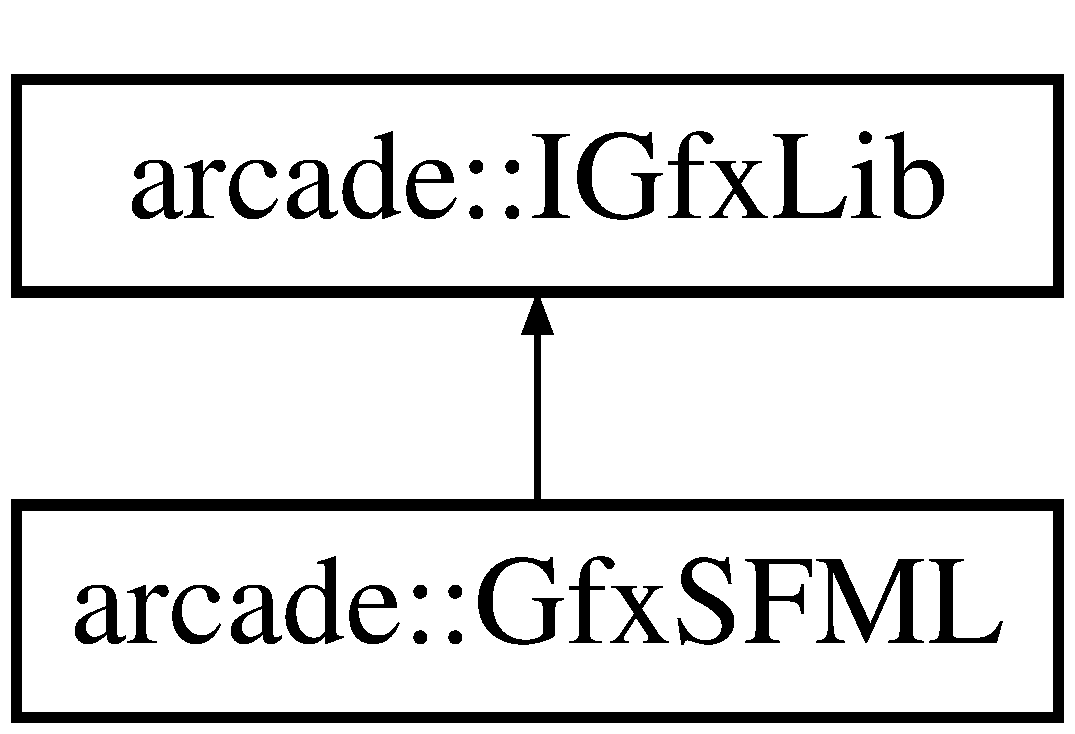
\includegraphics[height=2.000000cm]{classarcade_1_1_gfx_s_f_m_l}
\end{center}
\end{figure}
\subsection*{Public Member Functions}
\begin{DoxyCompactItemize}
\item 
virtual \hyperlink{classarcade_1_1_gfx_s_f_m_l_a66702cb942c775a31364c12fe5d6e06a}{$\sim$\+Gfx\+S\+F\+ML} ()
\item 
\hyperlink{classarcade_1_1_gfx_s_f_m_l_ad7ba5ca3fb9816b283a8603d6d28686f}{Gfx\+S\+F\+ML} ()
\item 
bool \hyperlink{classarcade_1_1_gfx_s_f_m_l_a7c2d800770d4218eb38c8b01f5890aa3}{poll\+Event} (\hyperlink{structarcade_1_1_event}{Event} \&e) override
\begin{DoxyCompactList}\small\item\em Function to poll events from the graphic lib. \end{DoxyCompactList}\item 
bool \hyperlink{classarcade_1_1_gfx_s_f_m_l_aa8d0f997c7ddcb68526e0f19f5bad77d}{does\+Support\+Sound} () const override
\begin{DoxyCompactList}\small\item\em Ask if the library support sound. \end{DoxyCompactList}\item 
void \hyperlink{classarcade_1_1_gfx_s_f_m_l_ad21d26a1e549e2da25da1c9f4155151c}{update\+Map} (\hyperlink{classarcade_1_1_i_map}{I\+Map} const \&map) override
\begin{DoxyCompactList}\small\item\em Update the map displayed. \end{DoxyCompactList}\item 
void \hyperlink{classarcade_1_1_gfx_s_f_m_l_a590d6b932d5200a1367d8a2ff76def61}{display} () override
\begin{DoxyCompactList}\small\item\em Display the map and \hyperlink{classarcade_1_1_g_u_i}{G\+UI}. \end{DoxyCompactList}\item 
void \hyperlink{classarcade_1_1_gfx_s_f_m_l_a12711203981dc2b9ce60df96d0aa6f55}{clear} () override
\begin{DoxyCompactList}\small\item\em Ask the lib to clear the screen. \end{DoxyCompactList}\item 
void \hyperlink{classarcade_1_1_gfx_s_f_m_l_aaec16dc42e480cdb6b6cbc3f75e4951c}{load\+Sounds} (std\+::vector$<$ std\+::pair$<$ std\+::string, \hyperlink{namespacearcade_a3bb4743a2eea59f3927e404e6549cae5}{Sound\+Type} $>$ $>$ const \&sounds) override
\begin{DoxyCompactList}\small\item\em Ask the lib to remove and load new sounds. \end{DoxyCompactList}\item 
void \hyperlink{classarcade_1_1_gfx_s_f_m_l_a785424b9463d487365c781bf91eda6a8}{sound\+Control} (const \hyperlink{structarcade_1_1_sound}{Sound} \&sound) override
\begin{DoxyCompactList}\small\item\em Ask the lib to play a sound. \end{DoxyCompactList}\item 
void \hyperlink{classarcade_1_1_gfx_s_f_m_l_a1e586ce151c47e3b5a6abcfdf5ecdc79}{load\+Sprites} (std\+::vector$<$ std\+::unique\+\_\+ptr$<$ \hyperlink{classarcade_1_1_i_sprite}{I\+Sprite} $>$$>$ \&\&sprites) override
\begin{DoxyCompactList}\small\item\em Load sprites in the lib from the paths given by the game. \end{DoxyCompactList}\item 
void \hyperlink{classarcade_1_1_gfx_s_f_m_l_ad8ba0c70b00c4132010ceabc2246bb59}{update\+G\+UI} (\hyperlink{classarcade_1_1_i_g_u_i}{I\+G\+UI} \&gui) override
\begin{DoxyCompactList}\small\item\em Update the \hyperlink{classarcade_1_1_g_u_i}{G\+UI} displayed. \end{DoxyCompactList}\end{DoxyCompactItemize}


\subsection{Constructor \& Destructor Documentation}
\mbox{\Hypertarget{classarcade_1_1_gfx_s_f_m_l_a66702cb942c775a31364c12fe5d6e06a}\label{classarcade_1_1_gfx_s_f_m_l_a66702cb942c775a31364c12fe5d6e06a}} 
\index{arcade\+::\+Gfx\+S\+F\+ML@{arcade\+::\+Gfx\+S\+F\+ML}!````~Gfx\+S\+F\+ML@{$\sim$\+Gfx\+S\+F\+ML}}
\index{````~Gfx\+S\+F\+ML@{$\sim$\+Gfx\+S\+F\+ML}!arcade\+::\+Gfx\+S\+F\+ML@{arcade\+::\+Gfx\+S\+F\+ML}}
\subsubsection{\texorpdfstring{$\sim$\+Gfx\+S\+F\+M\+L()}{~GfxSFML()}}
{\footnotesize\ttfamily arcade\+::\+Gfx\+S\+F\+M\+L\+::$\sim$\+Gfx\+S\+F\+ML (\begin{DoxyParamCaption}{ }\end{DoxyParamCaption})\hspace{0.3cm}{\ttfamily [virtual]}}

\mbox{\Hypertarget{classarcade_1_1_gfx_s_f_m_l_ad7ba5ca3fb9816b283a8603d6d28686f}\label{classarcade_1_1_gfx_s_f_m_l_ad7ba5ca3fb9816b283a8603d6d28686f}} 
\index{arcade\+::\+Gfx\+S\+F\+ML@{arcade\+::\+Gfx\+S\+F\+ML}!Gfx\+S\+F\+ML@{Gfx\+S\+F\+ML}}
\index{Gfx\+S\+F\+ML@{Gfx\+S\+F\+ML}!arcade\+::\+Gfx\+S\+F\+ML@{arcade\+::\+Gfx\+S\+F\+ML}}
\subsubsection{\texorpdfstring{Gfx\+S\+F\+M\+L()}{GfxSFML()}}
{\footnotesize\ttfamily arcade\+::\+Gfx\+S\+F\+M\+L\+::\+Gfx\+S\+F\+ML (\begin{DoxyParamCaption}{ }\end{DoxyParamCaption})}

A key

B key

C key

D key

E key

F key

G key

H key

I key

J key

K key

L key

M key

N key

O key

P key

Q key

R key

S key

T key

U key

V key

X key

Y key

Z key

0 key

1 key

2 key

3 key

4 key

5 key

6 key

7 key

8 key

9 key

Left arrow key

Right arrow key

Up arrow key

Down arrow key

Space key

Enter/\+Carriage return key

Backspace key

Left Control key

Right Control key

Left Alt key

Right Alt key

Left Shift key

Right Shift key

Tabulation key

Escape key

Page up key

Page down

Home key

End key

Function key 1 (F1)

Function key 2 (F2)

Function key 3 (F3)

Function key 4 (F4)

Function key 5 (F5)

Function key 6 (F6)

Function key 7 (F7)

Function key 8 (F8)

Function key 9 (F9)

Function key 10 (F10)

Function key 11 (F11)

Function key 12 (F12)

Comma key (,)

Dot (period) key (.)

Slash key (/)

Semicolon key (;)

Simple quote key (\textquotesingle{})

Left bracket key (\mbox{[})

Right bracker key (\mbox{]})

Backslash key ()

Asterisk key ($\ast$)

Minus symbol key (-\/)

Plus symbol key (+) 

\subsection{Member Function Documentation}
\mbox{\Hypertarget{classarcade_1_1_gfx_s_f_m_l_a12711203981dc2b9ce60df96d0aa6f55}\label{classarcade_1_1_gfx_s_f_m_l_a12711203981dc2b9ce60df96d0aa6f55}} 
\index{arcade\+::\+Gfx\+S\+F\+ML@{arcade\+::\+Gfx\+S\+F\+ML}!clear@{clear}}
\index{clear@{clear}!arcade\+::\+Gfx\+S\+F\+ML@{arcade\+::\+Gfx\+S\+F\+ML}}
\subsubsection{\texorpdfstring{clear()}{clear()}}
{\footnotesize\ttfamily void arcade\+::\+Gfx\+S\+F\+M\+L\+::clear (\begin{DoxyParamCaption}{ }\end{DoxyParamCaption})\hspace{0.3cm}{\ttfamily [override]}, {\ttfamily [virtual]}}



Ask the lib to clear the screen. 



Implements \hyperlink{classarcade_1_1_i_gfx_lib_a4116b3d4f503c4a795539b584f77a73d}{arcade\+::\+I\+Gfx\+Lib}.

\mbox{\Hypertarget{classarcade_1_1_gfx_s_f_m_l_a590d6b932d5200a1367d8a2ff76def61}\label{classarcade_1_1_gfx_s_f_m_l_a590d6b932d5200a1367d8a2ff76def61}} 
\index{arcade\+::\+Gfx\+S\+F\+ML@{arcade\+::\+Gfx\+S\+F\+ML}!display@{display}}
\index{display@{display}!arcade\+::\+Gfx\+S\+F\+ML@{arcade\+::\+Gfx\+S\+F\+ML}}
\subsubsection{\texorpdfstring{display()}{display()}}
{\footnotesize\ttfamily void arcade\+::\+Gfx\+S\+F\+M\+L\+::display (\begin{DoxyParamCaption}{ }\end{DoxyParamCaption})\hspace{0.3cm}{\ttfamily [override]}, {\ttfamily [virtual]}}



Display the map and \hyperlink{classarcade_1_1_g_u_i}{G\+UI}. 



Implements \hyperlink{classarcade_1_1_i_gfx_lib_a7f280525c718a44c1e05cfe0ba5304c3}{arcade\+::\+I\+Gfx\+Lib}.

\mbox{\Hypertarget{classarcade_1_1_gfx_s_f_m_l_aa8d0f997c7ddcb68526e0f19f5bad77d}\label{classarcade_1_1_gfx_s_f_m_l_aa8d0f997c7ddcb68526e0f19f5bad77d}} 
\index{arcade\+::\+Gfx\+S\+F\+ML@{arcade\+::\+Gfx\+S\+F\+ML}!does\+Support\+Sound@{does\+Support\+Sound}}
\index{does\+Support\+Sound@{does\+Support\+Sound}!arcade\+::\+Gfx\+S\+F\+ML@{arcade\+::\+Gfx\+S\+F\+ML}}
\subsubsection{\texorpdfstring{does\+Support\+Sound()}{doesSupportSound()}}
{\footnotesize\ttfamily bool arcade\+::\+Gfx\+S\+F\+M\+L\+::does\+Support\+Sound (\begin{DoxyParamCaption}{ }\end{DoxyParamCaption}) const\hspace{0.3cm}{\ttfamily [override]}, {\ttfamily [virtual]}}



Ask if the library support sound. 



Implements \hyperlink{classarcade_1_1_i_gfx_lib_a68cfbc987dfecca5b1405e36e00157b2}{arcade\+::\+I\+Gfx\+Lib}.

\mbox{\Hypertarget{classarcade_1_1_gfx_s_f_m_l_aaec16dc42e480cdb6b6cbc3f75e4951c}\label{classarcade_1_1_gfx_s_f_m_l_aaec16dc42e480cdb6b6cbc3f75e4951c}} 
\index{arcade\+::\+Gfx\+S\+F\+ML@{arcade\+::\+Gfx\+S\+F\+ML}!load\+Sounds@{load\+Sounds}}
\index{load\+Sounds@{load\+Sounds}!arcade\+::\+Gfx\+S\+F\+ML@{arcade\+::\+Gfx\+S\+F\+ML}}
\subsubsection{\texorpdfstring{load\+Sounds()}{loadSounds()}}
{\footnotesize\ttfamily void arcade\+::\+Gfx\+S\+F\+M\+L\+::load\+Sounds (\begin{DoxyParamCaption}\item[{std\+::vector$<$ std\+::pair$<$ std\+::string, \hyperlink{namespacearcade_a3bb4743a2eea59f3927e404e6549cae5}{Sound\+Type} $>$ $>$ const \&}]{sounds }\end{DoxyParamCaption})\hspace{0.3cm}{\ttfamily [override]}, {\ttfamily [virtual]}}



Ask the lib to remove and load new sounds. 



Implements \hyperlink{classarcade_1_1_i_gfx_lib_a725faf0722d284d15eb389b0a1891a27}{arcade\+::\+I\+Gfx\+Lib}.

\mbox{\Hypertarget{classarcade_1_1_gfx_s_f_m_l_a1e586ce151c47e3b5a6abcfdf5ecdc79}\label{classarcade_1_1_gfx_s_f_m_l_a1e586ce151c47e3b5a6abcfdf5ecdc79}} 
\index{arcade\+::\+Gfx\+S\+F\+ML@{arcade\+::\+Gfx\+S\+F\+ML}!load\+Sprites@{load\+Sprites}}
\index{load\+Sprites@{load\+Sprites}!arcade\+::\+Gfx\+S\+F\+ML@{arcade\+::\+Gfx\+S\+F\+ML}}
\subsubsection{\texorpdfstring{load\+Sprites()}{loadSprites()}}
{\footnotesize\ttfamily void arcade\+::\+Gfx\+S\+F\+M\+L\+::load\+Sprites (\begin{DoxyParamCaption}\item[{std\+::vector$<$ std\+::unique\+\_\+ptr$<$ \hyperlink{classarcade_1_1_i_sprite}{I\+Sprite} $>$$>$ \&\&}]{sprites }\end{DoxyParamCaption})\hspace{0.3cm}{\ttfamily [override]}, {\ttfamily [virtual]}}



Load sprites in the lib from the paths given by the game. 


\begin{DoxyParams}{Parameters}
{\em sprites} & to pass the path of your sprites to give your lib the way to search your assets \\
\hline
\end{DoxyParams}


Implements \hyperlink{classarcade_1_1_i_gfx_lib_ad5b301c8ff56c428971a2a006514b709}{arcade\+::\+I\+Gfx\+Lib}.

\mbox{\Hypertarget{classarcade_1_1_gfx_s_f_m_l_a7c2d800770d4218eb38c8b01f5890aa3}\label{classarcade_1_1_gfx_s_f_m_l_a7c2d800770d4218eb38c8b01f5890aa3}} 
\index{arcade\+::\+Gfx\+S\+F\+ML@{arcade\+::\+Gfx\+S\+F\+ML}!poll\+Event@{poll\+Event}}
\index{poll\+Event@{poll\+Event}!arcade\+::\+Gfx\+S\+F\+ML@{arcade\+::\+Gfx\+S\+F\+ML}}
\subsubsection{\texorpdfstring{poll\+Event()}{pollEvent()}}
{\footnotesize\ttfamily bool arcade\+::\+Gfx\+S\+F\+M\+L\+::poll\+Event (\begin{DoxyParamCaption}\item[{\hyperlink{structarcade_1_1_event}{arcade\+::\+Event} \&}]{e }\end{DoxyParamCaption})\hspace{0.3cm}{\ttfamily [override]}, {\ttfamily [virtual]}}



Function to poll events from the graphic lib. 

If there is an event to poll, e is filled and true is returned. If not, false is returned. 

Implements \hyperlink{classarcade_1_1_i_gfx_lib_a82cdd82f168ca898ef81edf82ca6147a}{arcade\+::\+I\+Gfx\+Lib}.

\mbox{\Hypertarget{classarcade_1_1_gfx_s_f_m_l_a785424b9463d487365c781bf91eda6a8}\label{classarcade_1_1_gfx_s_f_m_l_a785424b9463d487365c781bf91eda6a8}} 
\index{arcade\+::\+Gfx\+S\+F\+ML@{arcade\+::\+Gfx\+S\+F\+ML}!sound\+Control@{sound\+Control}}
\index{sound\+Control@{sound\+Control}!arcade\+::\+Gfx\+S\+F\+ML@{arcade\+::\+Gfx\+S\+F\+ML}}
\subsubsection{\texorpdfstring{sound\+Control()}{soundControl()}}
{\footnotesize\ttfamily void arcade\+::\+Gfx\+S\+F\+M\+L\+::sound\+Control (\begin{DoxyParamCaption}\item[{const \hyperlink{structarcade_1_1_sound}{Sound} \&}]{sound }\end{DoxyParamCaption})\hspace{0.3cm}{\ttfamily [override]}, {\ttfamily [virtual]}}



Ask the lib to play a sound. 



Implements \hyperlink{classarcade_1_1_i_gfx_lib_a0b965ed555739ef366b27583799d794c}{arcade\+::\+I\+Gfx\+Lib}.

\mbox{\Hypertarget{classarcade_1_1_gfx_s_f_m_l_ad8ba0c70b00c4132010ceabc2246bb59}\label{classarcade_1_1_gfx_s_f_m_l_ad8ba0c70b00c4132010ceabc2246bb59}} 
\index{arcade\+::\+Gfx\+S\+F\+ML@{arcade\+::\+Gfx\+S\+F\+ML}!update\+G\+UI@{update\+G\+UI}}
\index{update\+G\+UI@{update\+G\+UI}!arcade\+::\+Gfx\+S\+F\+ML@{arcade\+::\+Gfx\+S\+F\+ML}}
\subsubsection{\texorpdfstring{update\+G\+U\+I()}{updateGUI()}}
{\footnotesize\ttfamily void arcade\+::\+Gfx\+S\+F\+M\+L\+::update\+G\+UI (\begin{DoxyParamCaption}\item[{\hyperlink{classarcade_1_1_i_g_u_i}{I\+G\+UI} \&}]{gui }\end{DoxyParamCaption})\hspace{0.3cm}{\ttfamily [override]}, {\ttfamily [virtual]}}



Update the \hyperlink{classarcade_1_1_g_u_i}{G\+UI} displayed. 



Implements \hyperlink{classarcade_1_1_i_gfx_lib_ae3f443cc341512433815e8bf2dee3e0d}{arcade\+::\+I\+Gfx\+Lib}.

\mbox{\Hypertarget{classarcade_1_1_gfx_s_f_m_l_ad21d26a1e549e2da25da1c9f4155151c}\label{classarcade_1_1_gfx_s_f_m_l_ad21d26a1e549e2da25da1c9f4155151c}} 
\index{arcade\+::\+Gfx\+S\+F\+ML@{arcade\+::\+Gfx\+S\+F\+ML}!update\+Map@{update\+Map}}
\index{update\+Map@{update\+Map}!arcade\+::\+Gfx\+S\+F\+ML@{arcade\+::\+Gfx\+S\+F\+ML}}
\subsubsection{\texorpdfstring{update\+Map()}{updateMap()}}
{\footnotesize\ttfamily void arcade\+::\+Gfx\+S\+F\+M\+L\+::update\+Map (\begin{DoxyParamCaption}\item[{\hyperlink{classarcade_1_1_i_map}{I\+Map} const \&}]{map }\end{DoxyParamCaption})\hspace{0.3cm}{\ttfamily [override]}, {\ttfamily [virtual]}}



Update the map displayed. 



Implements \hyperlink{classarcade_1_1_i_gfx_lib_addc883f69b75e6ec4927027aad94f5b5}{arcade\+::\+I\+Gfx\+Lib}.



The documentation for this class was generated from the following files\+:\begin{DoxyCompactItemize}
\item 
gfx\+Libs\+Srcs/sfml/\hyperlink{_gfx_s_f_m_l_8hpp}{Gfx\+S\+F\+M\+L.\+hpp}\item 
gfx\+Libs\+Srcs/sfml/\hyperlink{_gfx_s_f_m_l_8cpp}{Gfx\+S\+F\+M\+L.\+cpp}\end{DoxyCompactItemize}

\hypertarget{classarcade_1_1_g_u_i}{}\section{arcade\+:\+:G\+UI Class Reference}
\label{classarcade_1_1_g_u_i}\index{arcade\+::\+G\+UI@{arcade\+::\+G\+UI}}


{\ttfamily \#include $<$G\+U\+I.\+hpp$>$}

Inheritance diagram for arcade\+:\+:G\+UI\+:\begin{figure}[H]
\begin{center}
\leavevmode
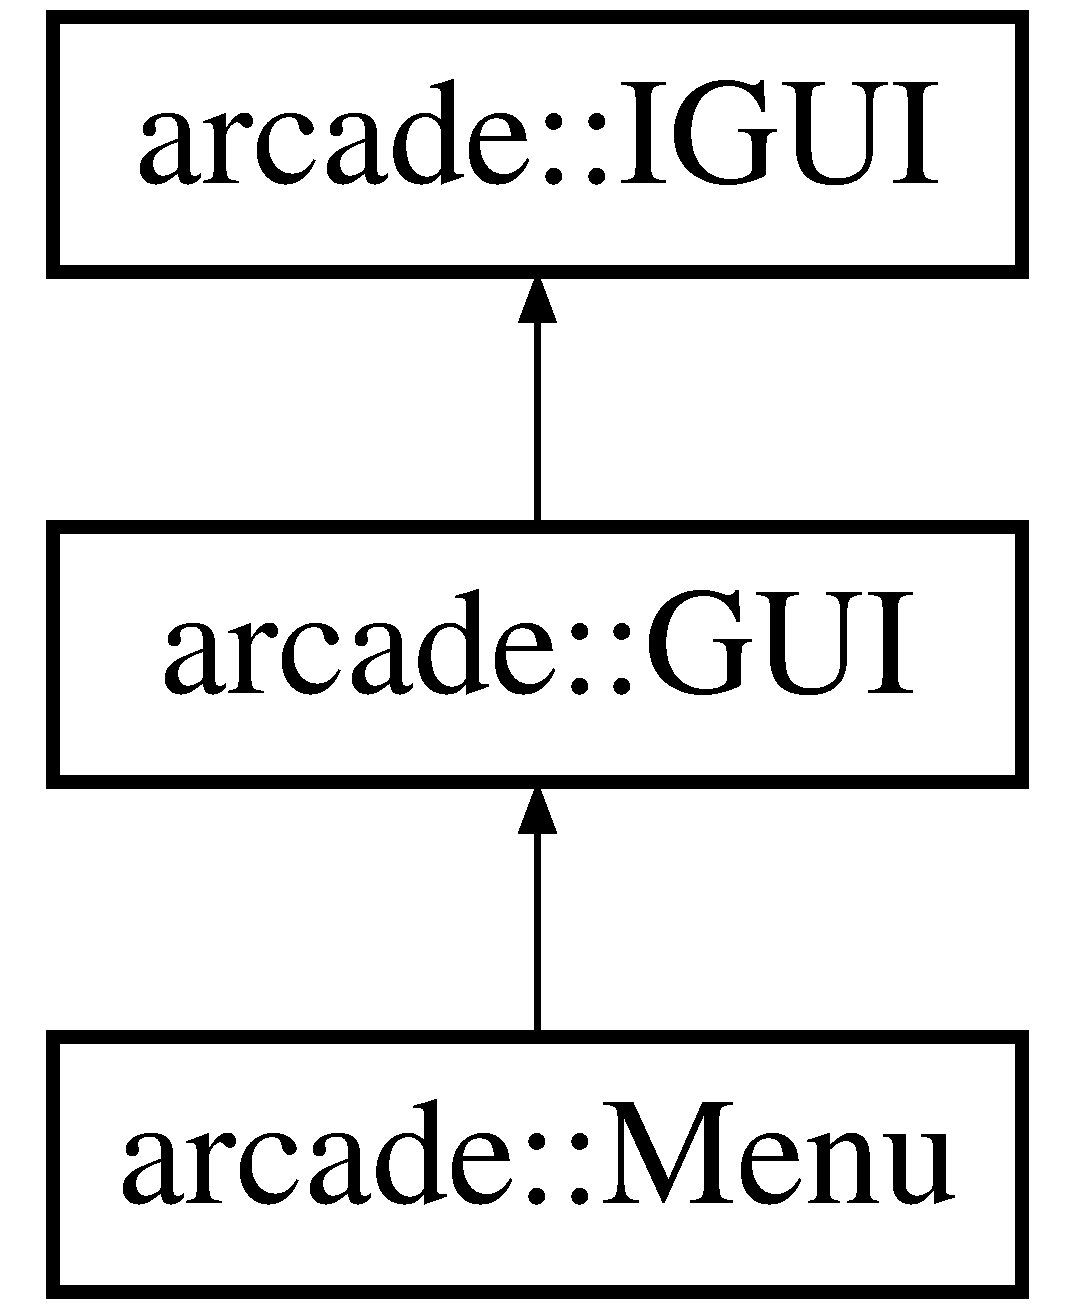
\includegraphics[height=3.000000cm]{classarcade_1_1_g_u_i}
\end{center}
\end{figure}
\subsection*{Public Member Functions}
\begin{DoxyCompactItemize}
\item 
virtual \hyperlink{classarcade_1_1_g_u_i_a303ab9f358e535d6e08bcf63a7175a96}{$\sim$\+G\+UI} ()
\item 
\hyperlink{classarcade_1_1_g_u_i_a320bdccbea68b4485ec98667735009d2}{G\+UI} ()
\item 
size\+\_\+t \hyperlink{classarcade_1_1_g_u_i_aa38b306ad674a221e0815cb600409598}{size} () const override
\begin{DoxyCompactList}\small\item\em Return the number of elements. \end{DoxyCompactList}\item 
\hyperlink{classarcade_1_1_i_component}{I\+Component} \& \hyperlink{classarcade_1_1_g_u_i_ab94910ea11fc43430227bfc716fd8c80}{at} (std\+::size\+\_\+t n) override
\begin{DoxyCompactList}\small\item\em Access to the n element. \end{DoxyCompactList}\item 
void \hyperlink{classarcade_1_1_g_u_i_aa6d6547eb12710f098d1a328f5eee7d4}{add\+Component} (\hyperlink{classarcade_1_1_u_i_component}{U\+I\+Component} $\ast$component)
\item 
virtual void \hyperlink{classarcade_1_1_g_u_i_abdf6ff80e7176b8a0e9c4561c5bfbf10}{update\+Components} ()
\end{DoxyCompactItemize}
\subsection*{Protected Attributes}
\begin{DoxyCompactItemize}
\item 
std\+::vector$<$ \hyperlink{classarcade_1_1_u_i_component}{U\+I\+Component} $\ast$ $>$ \hyperlink{classarcade_1_1_g_u_i_a190c384b099301972698f9bb410474de}{components}
\end{DoxyCompactItemize}


\subsection{Constructor \& Destructor Documentation}
\mbox{\Hypertarget{classarcade_1_1_g_u_i_a303ab9f358e535d6e08bcf63a7175a96}\label{classarcade_1_1_g_u_i_a303ab9f358e535d6e08bcf63a7175a96}} 
\index{arcade\+::\+G\+UI@{arcade\+::\+G\+UI}!````~G\+UI@{$\sim$\+G\+UI}}
\index{````~G\+UI@{$\sim$\+G\+UI}!arcade\+::\+G\+UI@{arcade\+::\+G\+UI}}
\subsubsection{\texorpdfstring{$\sim$\+G\+U\+I()}{~GUI()}}
{\footnotesize\ttfamily arcade\+::\+G\+U\+I\+::$\sim$\+G\+UI (\begin{DoxyParamCaption}{ }\end{DoxyParamCaption})\hspace{0.3cm}{\ttfamily [virtual]}}

\mbox{\Hypertarget{classarcade_1_1_g_u_i_a320bdccbea68b4485ec98667735009d2}\label{classarcade_1_1_g_u_i_a320bdccbea68b4485ec98667735009d2}} 
\index{arcade\+::\+G\+UI@{arcade\+::\+G\+UI}!G\+UI@{G\+UI}}
\index{G\+UI@{G\+UI}!arcade\+::\+G\+UI@{arcade\+::\+G\+UI}}
\subsubsection{\texorpdfstring{G\+U\+I()}{GUI()}}
{\footnotesize\ttfamily arcade\+::\+G\+U\+I\+::\+G\+UI (\begin{DoxyParamCaption}{ }\end{DoxyParamCaption})}



\subsection{Member Function Documentation}
\mbox{\Hypertarget{classarcade_1_1_g_u_i_aa6d6547eb12710f098d1a328f5eee7d4}\label{classarcade_1_1_g_u_i_aa6d6547eb12710f098d1a328f5eee7d4}} 
\index{arcade\+::\+G\+UI@{arcade\+::\+G\+UI}!add\+Component@{add\+Component}}
\index{add\+Component@{add\+Component}!arcade\+::\+G\+UI@{arcade\+::\+G\+UI}}
\subsubsection{\texorpdfstring{add\+Component()}{addComponent()}}
{\footnotesize\ttfamily void arcade\+::\+G\+U\+I\+::add\+Component (\begin{DoxyParamCaption}\item[{\hyperlink{classarcade_1_1_u_i_component}{arcade\+::\+U\+I\+Component} $\ast$}]{component }\end{DoxyParamCaption})}

\mbox{\Hypertarget{classarcade_1_1_g_u_i_ab94910ea11fc43430227bfc716fd8c80}\label{classarcade_1_1_g_u_i_ab94910ea11fc43430227bfc716fd8c80}} 
\index{arcade\+::\+G\+UI@{arcade\+::\+G\+UI}!at@{at}}
\index{at@{at}!arcade\+::\+G\+UI@{arcade\+::\+G\+UI}}
\subsubsection{\texorpdfstring{at()}{at()}}
{\footnotesize\ttfamily \hyperlink{classarcade_1_1_i_component}{arcade\+::\+I\+Component} \& arcade\+::\+G\+U\+I\+::at (\begin{DoxyParamCaption}\item[{std\+::size\+\_\+t}]{n }\end{DoxyParamCaption})\hspace{0.3cm}{\ttfamily [override]}, {\ttfamily [virtual]}}



Access to the n element. 



Implements \hyperlink{classarcade_1_1_i_g_u_i_aafde8788a75c98d0dfc1161e42e13558}{arcade\+::\+I\+G\+UI}.

\mbox{\Hypertarget{classarcade_1_1_g_u_i_aa38b306ad674a221e0815cb600409598}\label{classarcade_1_1_g_u_i_aa38b306ad674a221e0815cb600409598}} 
\index{arcade\+::\+G\+UI@{arcade\+::\+G\+UI}!size@{size}}
\index{size@{size}!arcade\+::\+G\+UI@{arcade\+::\+G\+UI}}
\subsubsection{\texorpdfstring{size()}{size()}}
{\footnotesize\ttfamily size\+\_\+t arcade\+::\+G\+U\+I\+::size (\begin{DoxyParamCaption}{ }\end{DoxyParamCaption}) const\hspace{0.3cm}{\ttfamily [override]}, {\ttfamily [virtual]}}



Return the number of elements. 



Implements \hyperlink{classarcade_1_1_i_g_u_i_a5e9b36772c4affcc58243880e6d51d62}{arcade\+::\+I\+G\+UI}.

\mbox{\Hypertarget{classarcade_1_1_g_u_i_abdf6ff80e7176b8a0e9c4561c5bfbf10}\label{classarcade_1_1_g_u_i_abdf6ff80e7176b8a0e9c4561c5bfbf10}} 
\index{arcade\+::\+G\+UI@{arcade\+::\+G\+UI}!update\+Components@{update\+Components}}
\index{update\+Components@{update\+Components}!arcade\+::\+G\+UI@{arcade\+::\+G\+UI}}
\subsubsection{\texorpdfstring{update\+Components()}{updateComponents()}}
{\footnotesize\ttfamily void arcade\+::\+G\+U\+I\+::update\+Components (\begin{DoxyParamCaption}{ }\end{DoxyParamCaption})\hspace{0.3cm}{\ttfamily [virtual]}}



Reimplemented in \hyperlink{classarcade_1_1_menu_a63906aaba91a3be7b0f4f8dcc46e87f4}{arcade\+::\+Menu}.



\subsection{Member Data Documentation}
\mbox{\Hypertarget{classarcade_1_1_g_u_i_a190c384b099301972698f9bb410474de}\label{classarcade_1_1_g_u_i_a190c384b099301972698f9bb410474de}} 
\index{arcade\+::\+G\+UI@{arcade\+::\+G\+UI}!components@{components}}
\index{components@{components}!arcade\+::\+G\+UI@{arcade\+::\+G\+UI}}
\subsubsection{\texorpdfstring{components}{components}}
{\footnotesize\ttfamily std\+::vector$<$\hyperlink{classarcade_1_1_u_i_component}{U\+I\+Component} $\ast$$>$ arcade\+::\+G\+U\+I\+::components\hspace{0.3cm}{\ttfamily [protected]}}



The documentation for this class was generated from the following files\+:\begin{DoxyCompactItemize}
\item 
include/\hyperlink{_g_u_i_8hpp}{G\+U\+I.\+hpp}\item 
srcs/\hyperlink{_g_u_i_8cpp}{G\+U\+I.\+cpp}\end{DoxyCompactItemize}

\hypertarget{classarcade_1_1_i_component}{}\section{arcade\+:\+:I\+Component Class Reference}
\label{classarcade_1_1_i_component}\index{arcade\+::\+I\+Component@{arcade\+::\+I\+Component}}


Interface used to manage \hyperlink{classarcade_1_1_g_u_i}{G\+UI} components.  




{\ttfamily \#include $<$I\+Component.\+hpp$>$}

Inheritance diagram for arcade\+:\+:I\+Component\+:\begin{figure}[H]
\begin{center}
\leavevmode
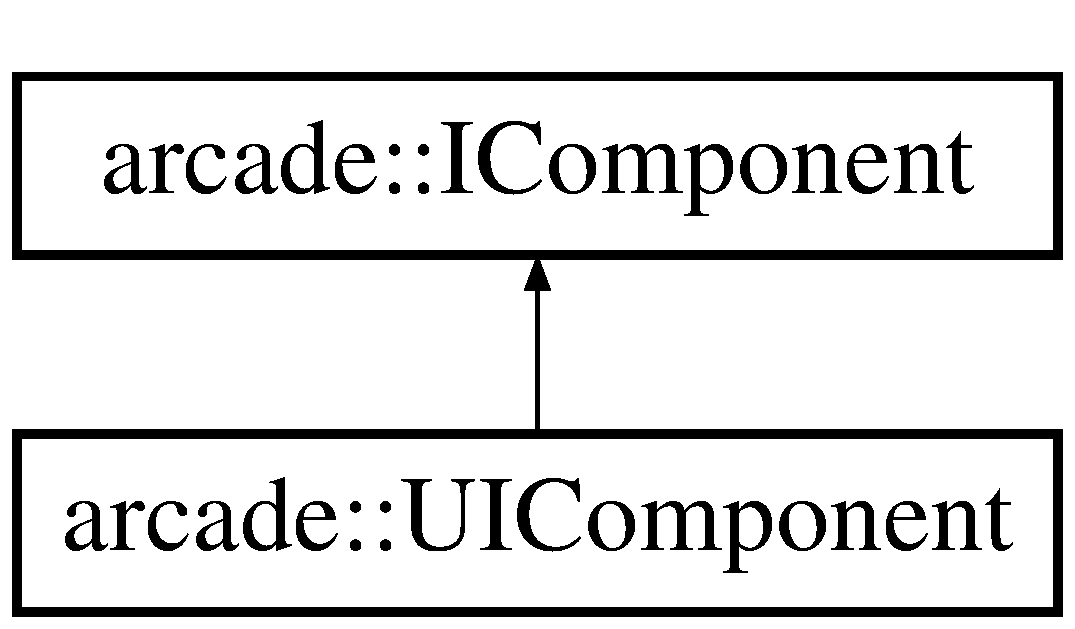
\includegraphics[height=2.000000cm]{classarcade_1_1_i_component}
\end{center}
\end{figure}
\subsection*{Public Member Functions}
\begin{DoxyCompactItemize}
\item 
virtual \hyperlink{classarcade_1_1_i_component_a1d4ec4990f66b23a90c4da6b00b3a32f}{$\sim$\+I\+Component} ()
\begin{DoxyCompactList}\small\item\em Virtual destructor of the interface. \end{DoxyCompactList}\item 
virtual double \hyperlink{classarcade_1_1_i_component_ab9d24992e8519756d56c0282001eccce}{getX} () const =0
\begin{DoxyCompactList}\small\item\em Get the X position (between 0.\+0 and 1.\+0) \end{DoxyCompactList}\item 
virtual double \hyperlink{classarcade_1_1_i_component_ad19f185c30ab99ed831d2c68fabf920f}{getY} () const =0
\begin{DoxyCompactList}\small\item\em Get the Y position (between 0.\+0 and 1.\+0) \end{DoxyCompactList}\item 
virtual double \hyperlink{classarcade_1_1_i_component_a558e5d49736a3828753a4062d5c9bfb1}{get\+Width} () const =0
\item 
virtual double \hyperlink{classarcade_1_1_i_component_a77a3bed39227f11d06bb71e06ee2ee30}{get\+Height} () const =0
\begin{DoxyCompactList}\small\item\em Get the component\textquotesingle{}s height (between 0.\+0 and 1.\+0) \end{DoxyCompactList}\item 
virtual bool \hyperlink{classarcade_1_1_i_component_a03ea8019a23fd44731a06548ef7e6ff3}{has\+Sprite} () const =0
\begin{DoxyCompactList}\small\item\em Return true if the component has a sprite. \end{DoxyCompactList}\item 
virtual size\+\_\+t \hyperlink{classarcade_1_1_i_component_a7d4c00172b0ba0e3dc63832a9234efbb}{get\+Background\+Id} () const =0
\begin{DoxyCompactList}\small\item\em Get the id of the background sprite. \end{DoxyCompactList}\item 
virtual \hyperlink{unionarcade_1_1_color}{Color} \hyperlink{classarcade_1_1_i_component_a99301c61be2a21ef8a274727ba781a00}{get\+Background\+Color} () const =0
\begin{DoxyCompactList}\small\item\em Get the color of the background. \end{DoxyCompactList}\item 
virtual \hyperlink{unionarcade_1_1_color}{Color} \hyperlink{classarcade_1_1_i_component_a9d4c57ad7c49e39ef0269f10fdc14807}{get\+Text\+Color} () const =0
\item 
virtual std\+::string const  \& \hyperlink{classarcade_1_1_i_component_a7c09ef60e3d41d4afedf2be77fe880a7}{get\+Text} () const =0
\begin{DoxyCompactList}\small\item\em Get the text value. \end{DoxyCompactList}\item 
virtual void \hyperlink{classarcade_1_1_i_component_ae0cd9b58ad0b127c671a5d8f92d9c25f}{set\+Clicked} ()=0
\begin{DoxyCompactList}\small\item\em Way of the lib to tell a component it was clicked. \end{DoxyCompactList}\end{DoxyCompactItemize}


\subsection{Detailed Description}
Interface used to manage \hyperlink{classarcade_1_1_g_u_i}{G\+UI} components. 

\subsection{Constructor \& Destructor Documentation}
\mbox{\Hypertarget{classarcade_1_1_i_component_a1d4ec4990f66b23a90c4da6b00b3a32f}\label{classarcade_1_1_i_component_a1d4ec4990f66b23a90c4da6b00b3a32f}} 
\index{arcade\+::\+I\+Component@{arcade\+::\+I\+Component}!````~I\+Component@{$\sim$\+I\+Component}}
\index{````~I\+Component@{$\sim$\+I\+Component}!arcade\+::\+I\+Component@{arcade\+::\+I\+Component}}
\subsubsection{\texorpdfstring{$\sim$\+I\+Component()}{~IComponent()}}
{\footnotesize\ttfamily arcade\+::\+I\+Component\+::$\sim$\+I\+Component (\begin{DoxyParamCaption}{ }\end{DoxyParamCaption})\hspace{0.3cm}{\ttfamily [inline]}, {\ttfamily [virtual]}}



Virtual destructor of the interface. 



\subsection{Member Function Documentation}
\mbox{\Hypertarget{classarcade_1_1_i_component_a99301c61be2a21ef8a274727ba781a00}\label{classarcade_1_1_i_component_a99301c61be2a21ef8a274727ba781a00}} 
\index{arcade\+::\+I\+Component@{arcade\+::\+I\+Component}!get\+Background\+Color@{get\+Background\+Color}}
\index{get\+Background\+Color@{get\+Background\+Color}!arcade\+::\+I\+Component@{arcade\+::\+I\+Component}}
\subsubsection{\texorpdfstring{get\+Background\+Color()}{getBackgroundColor()}}
{\footnotesize\ttfamily \hyperlink{unionarcade_1_1_color}{Color} arcade\+::\+I\+Component\+::get\+Background\+Color (\begin{DoxyParamCaption}{ }\end{DoxyParamCaption}) const\hspace{0.3cm}{\ttfamily [pure virtual]}}



Get the color of the background. 



Implemented in \hyperlink{classarcade_1_1_u_i_component_a981bbd394540b39ca0c7c0f760ef9551}{arcade\+::\+U\+I\+Component}.

\mbox{\Hypertarget{classarcade_1_1_i_component_a7d4c00172b0ba0e3dc63832a9234efbb}\label{classarcade_1_1_i_component_a7d4c00172b0ba0e3dc63832a9234efbb}} 
\index{arcade\+::\+I\+Component@{arcade\+::\+I\+Component}!get\+Background\+Id@{get\+Background\+Id}}
\index{get\+Background\+Id@{get\+Background\+Id}!arcade\+::\+I\+Component@{arcade\+::\+I\+Component}}
\subsubsection{\texorpdfstring{get\+Background\+Id()}{getBackgroundId()}}
{\footnotesize\ttfamily size\+\_\+t arcade\+::\+I\+Component\+::get\+Background\+Id (\begin{DoxyParamCaption}{ }\end{DoxyParamCaption}) const\hspace{0.3cm}{\ttfamily [pure virtual]}}



Get the id of the background sprite. 



Implemented in \hyperlink{classarcade_1_1_u_i_component_a7da87b1ce3bc56dcc6600e1c27e325a6}{arcade\+::\+U\+I\+Component}.

\mbox{\Hypertarget{classarcade_1_1_i_component_a77a3bed39227f11d06bb71e06ee2ee30}\label{classarcade_1_1_i_component_a77a3bed39227f11d06bb71e06ee2ee30}} 
\index{arcade\+::\+I\+Component@{arcade\+::\+I\+Component}!get\+Height@{get\+Height}}
\index{get\+Height@{get\+Height}!arcade\+::\+I\+Component@{arcade\+::\+I\+Component}}
\subsubsection{\texorpdfstring{get\+Height()}{getHeight()}}
{\footnotesize\ttfamily double arcade\+::\+I\+Component\+::get\+Height (\begin{DoxyParamCaption}{ }\end{DoxyParamCaption}) const\hspace{0.3cm}{\ttfamily [pure virtual]}}



Get the component\textquotesingle{}s height (between 0.\+0 and 1.\+0) 



Implemented in \hyperlink{classarcade_1_1_u_i_component_abb02d0b9324eabf8ddf0d1302a0b08f7}{arcade\+::\+U\+I\+Component}.

\mbox{\Hypertarget{classarcade_1_1_i_component_a7c09ef60e3d41d4afedf2be77fe880a7}\label{classarcade_1_1_i_component_a7c09ef60e3d41d4afedf2be77fe880a7}} 
\index{arcade\+::\+I\+Component@{arcade\+::\+I\+Component}!get\+Text@{get\+Text}}
\index{get\+Text@{get\+Text}!arcade\+::\+I\+Component@{arcade\+::\+I\+Component}}
\subsubsection{\texorpdfstring{get\+Text()}{getText()}}
{\footnotesize\ttfamily std\+::string const  \& arcade\+::\+I\+Component\+::get\+Text (\begin{DoxyParamCaption}{ }\end{DoxyParamCaption}) const\hspace{0.3cm}{\ttfamily [pure virtual]}}



Get the text value. 



Implemented in \hyperlink{classarcade_1_1_u_i_component_aa930897f9456ed9462063481d19d10ed}{arcade\+::\+U\+I\+Component}.

\mbox{\Hypertarget{classarcade_1_1_i_component_a9d4c57ad7c49e39ef0269f10fdc14807}\label{classarcade_1_1_i_component_a9d4c57ad7c49e39ef0269f10fdc14807}} 
\index{arcade\+::\+I\+Component@{arcade\+::\+I\+Component}!get\+Text\+Color@{get\+Text\+Color}}
\index{get\+Text\+Color@{get\+Text\+Color}!arcade\+::\+I\+Component@{arcade\+::\+I\+Component}}
\subsubsection{\texorpdfstring{get\+Text\+Color()}{getTextColor()}}
{\footnotesize\ttfamily virtual \hyperlink{unionarcade_1_1_color}{Color} arcade\+::\+I\+Component\+::get\+Text\+Color (\begin{DoxyParamCaption}{ }\end{DoxyParamCaption}) const\hspace{0.3cm}{\ttfamily [pure virtual]}}



Implemented in \hyperlink{classarcade_1_1_u_i_component_a0a9e2a34357ad6759d580e152a20adee}{arcade\+::\+U\+I\+Component}.

\mbox{\Hypertarget{classarcade_1_1_i_component_a558e5d49736a3828753a4062d5c9bfb1}\label{classarcade_1_1_i_component_a558e5d49736a3828753a4062d5c9bfb1}} 
\index{arcade\+::\+I\+Component@{arcade\+::\+I\+Component}!get\+Width@{get\+Width}}
\index{get\+Width@{get\+Width}!arcade\+::\+I\+Component@{arcade\+::\+I\+Component}}
\subsubsection{\texorpdfstring{get\+Width()}{getWidth()}}
{\footnotesize\ttfamily virtual double arcade\+::\+I\+Component\+::get\+Width (\begin{DoxyParamCaption}{ }\end{DoxyParamCaption}) const\hspace{0.3cm}{\ttfamily [pure virtual]}}



Implemented in \hyperlink{classarcade_1_1_u_i_component_a56c4ce3124813be5d456aec399c63bc9}{arcade\+::\+U\+I\+Component}.

\mbox{\Hypertarget{classarcade_1_1_i_component_ab9d24992e8519756d56c0282001eccce}\label{classarcade_1_1_i_component_ab9d24992e8519756d56c0282001eccce}} 
\index{arcade\+::\+I\+Component@{arcade\+::\+I\+Component}!getX@{getX}}
\index{getX@{getX}!arcade\+::\+I\+Component@{arcade\+::\+I\+Component}}
\subsubsection{\texorpdfstring{get\+X()}{getX()}}
{\footnotesize\ttfamily double arcade\+::\+I\+Component\+::getX (\begin{DoxyParamCaption}{ }\end{DoxyParamCaption}) const\hspace{0.3cm}{\ttfamily [pure virtual]}}



Get the X position (between 0.\+0 and 1.\+0) 



Implemented in \hyperlink{classarcade_1_1_u_i_component_a8da01c706810692c7c3f0711c957fb15}{arcade\+::\+U\+I\+Component}.

\mbox{\Hypertarget{classarcade_1_1_i_component_ad19f185c30ab99ed831d2c68fabf920f}\label{classarcade_1_1_i_component_ad19f185c30ab99ed831d2c68fabf920f}} 
\index{arcade\+::\+I\+Component@{arcade\+::\+I\+Component}!getY@{getY}}
\index{getY@{getY}!arcade\+::\+I\+Component@{arcade\+::\+I\+Component}}
\subsubsection{\texorpdfstring{get\+Y()}{getY()}}
{\footnotesize\ttfamily double arcade\+::\+I\+Component\+::getY (\begin{DoxyParamCaption}{ }\end{DoxyParamCaption}) const\hspace{0.3cm}{\ttfamily [pure virtual]}}



Get the Y position (between 0.\+0 and 1.\+0) 



Implemented in \hyperlink{classarcade_1_1_u_i_component_af5360eec3a1a473484df1df5f7d89ee9}{arcade\+::\+U\+I\+Component}.

\mbox{\Hypertarget{classarcade_1_1_i_component_a03ea8019a23fd44731a06548ef7e6ff3}\label{classarcade_1_1_i_component_a03ea8019a23fd44731a06548ef7e6ff3}} 
\index{arcade\+::\+I\+Component@{arcade\+::\+I\+Component}!has\+Sprite@{has\+Sprite}}
\index{has\+Sprite@{has\+Sprite}!arcade\+::\+I\+Component@{arcade\+::\+I\+Component}}
\subsubsection{\texorpdfstring{has\+Sprite()}{hasSprite()}}
{\footnotesize\ttfamily bool arcade\+::\+I\+Component\+::has\+Sprite (\begin{DoxyParamCaption}{ }\end{DoxyParamCaption}) const\hspace{0.3cm}{\ttfamily [pure virtual]}}



Return true if the component has a sprite. 



Implemented in \hyperlink{classarcade_1_1_u_i_component_a0f41ff1be1ae457a3be0856553e904f4}{arcade\+::\+U\+I\+Component}.

\mbox{\Hypertarget{classarcade_1_1_i_component_ae0cd9b58ad0b127c671a5d8f92d9c25f}\label{classarcade_1_1_i_component_ae0cd9b58ad0b127c671a5d8f92d9c25f}} 
\index{arcade\+::\+I\+Component@{arcade\+::\+I\+Component}!set\+Clicked@{set\+Clicked}}
\index{set\+Clicked@{set\+Clicked}!arcade\+::\+I\+Component@{arcade\+::\+I\+Component}}
\subsubsection{\texorpdfstring{set\+Clicked()}{setClicked()}}
{\footnotesize\ttfamily void arcade\+::\+I\+Component\+::set\+Clicked (\begin{DoxyParamCaption}{ }\end{DoxyParamCaption})\hspace{0.3cm}{\ttfamily [pure virtual]}}



Way of the lib to tell a component it was clicked. 



Implemented in \hyperlink{classarcade_1_1_u_i_component_a8d87597d38fbc7cd93835d5712e3915c}{arcade\+::\+U\+I\+Component}.



The documentation for this class was generated from the following file\+:\begin{DoxyCompactItemize}
\item 
arcade\+Interfaces/\hyperlink{_i_component_8hpp}{I\+Component.\+hpp}\end{DoxyCompactItemize}

\hypertarget{classarcade_1_1_i_game}{}\section{arcade\+:\+:I\+Game Class Reference}
\label{classarcade_1_1_i_game}\index{arcade\+::\+I\+Game@{arcade\+::\+I\+Game}}


Interface of a game for the \hyperlink{classarcade_1_1_core}{Core} program.  




{\ttfamily \#include $<$I\+Game.\+hpp$>$}

Inheritance diagram for arcade\+:\+:I\+Game\+:\begin{figure}[H]
\begin{center}
\leavevmode
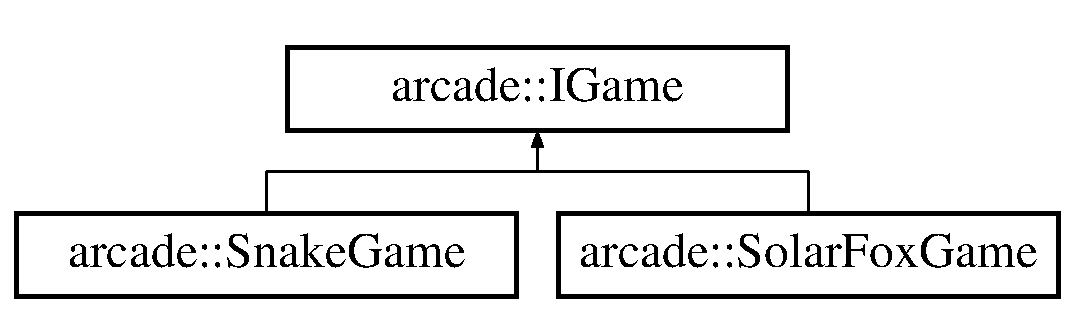
\includegraphics[height=2.000000cm]{classarcade_1_1_i_game}
\end{center}
\end{figure}
\subsection*{Public Member Functions}
\begin{DoxyCompactItemize}
\item 
virtual \hyperlink{classarcade_1_1_i_game_a89114f708822e3d0db5b58901c1e2354}{$\sim$\+I\+Game} ()
\begin{DoxyCompactList}\small\item\em Virtual destructor of the interface. \end{DoxyCompactList}\item 
virtual \hyperlink{namespacearcade_a6adca89ee2f539b03980c7e59b044ed7}{Game\+State} \hyperlink{classarcade_1_1_i_game_a75083f0465c0ccbdbbb38c689b4a694c}{get\+Game\+State} () const =0
\begin{DoxyCompactList}\small\item\em Ask the current game state to the game. \end{DoxyCompactList}\item 
virtual void \hyperlink{classarcade_1_1_i_game_a37d164b4052fa3c28256fb0bf0002876}{notify\+Event} (std\+::vector$<$ \hyperlink{structarcade_1_1_event}{Event} $>$ \&\&events)=0
\begin{DoxyCompactList}\small\item\em Send events (keyboard, mouse, etc) to the game. \end{DoxyCompactList}\item 
virtual void \hyperlink{classarcade_1_1_i_game_aaf375290947abf3db32d966facbfacf3}{notify\+Network} (std\+::vector$<$ \hyperlink{structarcade_1_1_network_packet}{Network\+Packet} $>$ \&\&events)=0
\begin{DoxyCompactList}\small\item\em Send network packets to the game. \end{DoxyCompactList}\item 
virtual std\+::vector$<$ \hyperlink{structarcade_1_1_network_packet}{Network\+Packet} $>$ \hyperlink{classarcade_1_1_i_game_a5aa80dfdb3c1881fbc749e3d53efc6f8}{get\+Network\+To\+Send} ()=0
\begin{DoxyCompactList}\small\item\em Get the network packet to send from the game to the server. \end{DoxyCompactList}\item 
virtual bool \hyperlink{classarcade_1_1_i_game_ae66bf253e252f43ce17d9e94f08a1d1c}{has\+Network} () const =0
\begin{DoxyCompactList}\small\item\em Does this game support network ? \end{DoxyCompactList}\item 
virtual void \hyperlink{classarcade_1_1_i_game_af0111a41083f38a1af1a7f94287e6e77}{process} ()=0
\begin{DoxyCompactList}\small\item\em Make the game process a game loop. \end{DoxyCompactList}\item 
virtual std\+::vector$<$ std\+::unique\+\_\+ptr$<$ \hyperlink{classarcade_1_1_i_sprite}{I\+Sprite} $>$ $>$ \hyperlink{classarcade_1_1_i_game_a2d0dc7c78a68c4dd0359911775993f68}{get\+Sprites\+To\+Load} () const =0
\begin{DoxyCompactList}\small\item\em get the list of sprites to load for this game \end{DoxyCompactList}\item 
virtual std\+::vector$<$ std\+::pair$<$ std\+::string, \hyperlink{namespacearcade_a3bb4743a2eea59f3927e404e6549cae5}{Sound\+Type} $>$ $>$ \hyperlink{classarcade_1_1_i_game_a0b66cd9ef3b5cd0dff95debb7e4f594e}{get\+Sounds\+To\+Load} () const =0
\begin{DoxyCompactList}\small\item\em get the list of sound files to load for this game \end{DoxyCompactList}\item 
virtual std\+::vector$<$ \hyperlink{structarcade_1_1_sound}{Sound} $>$ \hyperlink{classarcade_1_1_i_game_a88b3c7efb13780cdbbdf5b879a18ed4d}{get\+Sounds\+To\+Play} ()=0
\begin{DoxyCompactList}\small\item\em Get the sounds to play You should return by std\+::move to not copy your vector and to clear it at the same time. \end{DoxyCompactList}\item 
virtual \hyperlink{classarcade_1_1_i_map}{I\+Map} const  \& \hyperlink{classarcade_1_1_i_game_a2e1791071bf65ee35e249e409ee29044}{get\+Current\+Map} () const =0
\begin{DoxyCompactList}\small\item\em Get the current version of the map. \end{DoxyCompactList}\item 
virtual \hyperlink{classarcade_1_1_i_g_u_i}{I\+G\+UI} \& \hyperlink{classarcade_1_1_i_game_abe849a6ed370a18de51bc8cb7a2329ba}{get\+G\+UI} ()=0
\begin{DoxyCompactList}\small\item\em Get the current version of the \hyperlink{classarcade_1_1_g_u_i}{G\+UI} to display. \end{DoxyCompactList}\end{DoxyCompactItemize}


\subsection{Detailed Description}
Interface of a game for the \hyperlink{classarcade_1_1_core}{Core} program. 

This interface will be used by the \hyperlink{classarcade_1_1_core}{Core} program to manipulate a game without knowing any detail about it The \hyperlink{classarcade_1_1_core}{Core} will always do \char`\"{}request\char`\"{} to the game, to get information or ask for processing a game loop, for example. The \hyperlink{classarcade_1_1_i_game}{I\+Game} will never have a reference to the \hyperlink{classarcade_1_1_core}{Core}, or communicate directly with it. Never. Ever. 

\subsection{Constructor \& Destructor Documentation}
\mbox{\Hypertarget{classarcade_1_1_i_game_a89114f708822e3d0db5b58901c1e2354}\label{classarcade_1_1_i_game_a89114f708822e3d0db5b58901c1e2354}} 
\index{arcade\+::\+I\+Game@{arcade\+::\+I\+Game}!````~I\+Game@{$\sim$\+I\+Game}}
\index{````~I\+Game@{$\sim$\+I\+Game}!arcade\+::\+I\+Game@{arcade\+::\+I\+Game}}
\subsubsection{\texorpdfstring{$\sim$\+I\+Game()}{~IGame()}}
{\footnotesize\ttfamily arcade\+::\+I\+Game\+::$\sim$\+I\+Game (\begin{DoxyParamCaption}{ }\end{DoxyParamCaption})\hspace{0.3cm}{\ttfamily [inline]}, {\ttfamily [virtual]}}



Virtual destructor of the interface. 



\subsection{Member Function Documentation}
\mbox{\Hypertarget{classarcade_1_1_i_game_a2e1791071bf65ee35e249e409ee29044}\label{classarcade_1_1_i_game_a2e1791071bf65ee35e249e409ee29044}} 
\index{arcade\+::\+I\+Game@{arcade\+::\+I\+Game}!get\+Current\+Map@{get\+Current\+Map}}
\index{get\+Current\+Map@{get\+Current\+Map}!arcade\+::\+I\+Game@{arcade\+::\+I\+Game}}
\subsubsection{\texorpdfstring{get\+Current\+Map()}{getCurrentMap()}}
{\footnotesize\ttfamily \hyperlink{classarcade_1_1_i_map}{I\+Map} const  \& arcade\+::\+I\+Game\+::get\+Current\+Map (\begin{DoxyParamCaption}{ }\end{DoxyParamCaption}) const\hspace{0.3cm}{\ttfamily [pure virtual]}}



Get the current version of the map. 



Implemented in \hyperlink{classarcade_1_1_solar_fox_game_a8bb422466d4367320e90c6f9c6b754ed}{arcade\+::\+Solar\+Fox\+Game}, and \hyperlink{classarcade_1_1_snake_game_abc3fe4beaa1d2b7df8573f3375cbd4cb}{arcade\+::\+Snake\+Game}.

\mbox{\Hypertarget{classarcade_1_1_i_game_a75083f0465c0ccbdbbb38c689b4a694c}\label{classarcade_1_1_i_game_a75083f0465c0ccbdbbb38c689b4a694c}} 
\index{arcade\+::\+I\+Game@{arcade\+::\+I\+Game}!get\+Game\+State@{get\+Game\+State}}
\index{get\+Game\+State@{get\+Game\+State}!arcade\+::\+I\+Game@{arcade\+::\+I\+Game}}
\subsubsection{\texorpdfstring{get\+Game\+State()}{getGameState()}}
{\footnotesize\ttfamily \hyperlink{namespacearcade_a6adca89ee2f539b03980c7e59b044ed7}{Game\+State} arcade\+::\+I\+Game\+::get\+Game\+State (\begin{DoxyParamCaption}{ }\end{DoxyParamCaption}) const\hspace{0.3cm}{\ttfamily [pure virtual]}}



Ask the current game state to the game. 



Implemented in \hyperlink{classarcade_1_1_solar_fox_game_a71122936c223e672058280755f24a98a}{arcade\+::\+Solar\+Fox\+Game}, and \hyperlink{classarcade_1_1_snake_game_afcd7d113f2187cd34396022af4e9e10c}{arcade\+::\+Snake\+Game}.

\mbox{\Hypertarget{classarcade_1_1_i_game_abe849a6ed370a18de51bc8cb7a2329ba}\label{classarcade_1_1_i_game_abe849a6ed370a18de51bc8cb7a2329ba}} 
\index{arcade\+::\+I\+Game@{arcade\+::\+I\+Game}!get\+G\+UI@{get\+G\+UI}}
\index{get\+G\+UI@{get\+G\+UI}!arcade\+::\+I\+Game@{arcade\+::\+I\+Game}}
\subsubsection{\texorpdfstring{get\+G\+U\+I()}{getGUI()}}
{\footnotesize\ttfamily \hyperlink{classarcade_1_1_i_g_u_i}{I\+G\+UI} \& arcade\+::\+I\+Game\+::get\+G\+UI (\begin{DoxyParamCaption}{ }\end{DoxyParamCaption})\hspace{0.3cm}{\ttfamily [pure virtual]}}



Get the current version of the \hyperlink{classarcade_1_1_g_u_i}{G\+UI} to display. 



Implemented in \hyperlink{classarcade_1_1_solar_fox_game_aba8a5d93b17231c5d2cbbb51cc1d05b9}{arcade\+::\+Solar\+Fox\+Game}, and \hyperlink{classarcade_1_1_snake_game_ab586312d56bab5be7e1506fa513fea44}{arcade\+::\+Snake\+Game}.

\mbox{\Hypertarget{classarcade_1_1_i_game_a5aa80dfdb3c1881fbc749e3d53efc6f8}\label{classarcade_1_1_i_game_a5aa80dfdb3c1881fbc749e3d53efc6f8}} 
\index{arcade\+::\+I\+Game@{arcade\+::\+I\+Game}!get\+Network\+To\+Send@{get\+Network\+To\+Send}}
\index{get\+Network\+To\+Send@{get\+Network\+To\+Send}!arcade\+::\+I\+Game@{arcade\+::\+I\+Game}}
\subsubsection{\texorpdfstring{get\+Network\+To\+Send()}{getNetworkToSend()}}
{\footnotesize\ttfamily std\+::vector$<$ \hyperlink{structarcade_1_1_network_packet}{Network\+Packet} $>$ \&\& arcade\+::\+I\+Game\+::get\+Network\+To\+Send (\begin{DoxyParamCaption}{ }\end{DoxyParamCaption})\hspace{0.3cm}{\ttfamily [pure virtual]}}



Get the network packet to send from the game to the server. 



Implemented in \hyperlink{classarcade_1_1_solar_fox_game_a54b56444f83661b4330de868024671d6}{arcade\+::\+Solar\+Fox\+Game}, and \hyperlink{classarcade_1_1_snake_game_a8666c3ad148b7140658b52a262bfab73}{arcade\+::\+Snake\+Game}.

\mbox{\Hypertarget{classarcade_1_1_i_game_a0b66cd9ef3b5cd0dff95debb7e4f594e}\label{classarcade_1_1_i_game_a0b66cd9ef3b5cd0dff95debb7e4f594e}} 
\index{arcade\+::\+I\+Game@{arcade\+::\+I\+Game}!get\+Sounds\+To\+Load@{get\+Sounds\+To\+Load}}
\index{get\+Sounds\+To\+Load@{get\+Sounds\+To\+Load}!arcade\+::\+I\+Game@{arcade\+::\+I\+Game}}
\subsubsection{\texorpdfstring{get\+Sounds\+To\+Load()}{getSoundsToLoad()}}
{\footnotesize\ttfamily std\+::vector$<$ std\+::string $>$ arcade\+::\+I\+Game\+::get\+Sounds\+To\+Load (\begin{DoxyParamCaption}{ }\end{DoxyParamCaption}) const\hspace{0.3cm}{\ttfamily [pure virtual]}}



get the list of sound files to load for this game 



Implemented in \hyperlink{classarcade_1_1_solar_fox_game_aed75a8fdc63d9162359ada5332b44331}{arcade\+::\+Solar\+Fox\+Game}, and \hyperlink{classarcade_1_1_snake_game_a2d8ca7114ab012187da99658a221fab9}{arcade\+::\+Snake\+Game}.

\mbox{\Hypertarget{classarcade_1_1_i_game_a88b3c7efb13780cdbbdf5b879a18ed4d}\label{classarcade_1_1_i_game_a88b3c7efb13780cdbbdf5b879a18ed4d}} 
\index{arcade\+::\+I\+Game@{arcade\+::\+I\+Game}!get\+Sounds\+To\+Play@{get\+Sounds\+To\+Play}}
\index{get\+Sounds\+To\+Play@{get\+Sounds\+To\+Play}!arcade\+::\+I\+Game@{arcade\+::\+I\+Game}}
\subsubsection{\texorpdfstring{get\+Sounds\+To\+Play()}{getSoundsToPlay()}}
{\footnotesize\ttfamily std\+::vector$<$ \hyperlink{structarcade_1_1_sound}{Sound} $>$ arcade\+::\+I\+Game\+::get\+Sounds\+To\+Play (\begin{DoxyParamCaption}{ }\end{DoxyParamCaption})\hspace{0.3cm}{\ttfamily [pure virtual]}}



Get the sounds to play You should return by std\+::move to not copy your vector and to clear it at the same time. 



Implemented in \hyperlink{classarcade_1_1_solar_fox_game_a96f41df94a733d0c06f8a7d48e620d58}{arcade\+::\+Solar\+Fox\+Game}, and \hyperlink{classarcade_1_1_snake_game_aab993e72ca1b68914c37209781a68835}{arcade\+::\+Snake\+Game}.

\mbox{\Hypertarget{classarcade_1_1_i_game_a2d0dc7c78a68c4dd0359911775993f68}\label{classarcade_1_1_i_game_a2d0dc7c78a68c4dd0359911775993f68}} 
\index{arcade\+::\+I\+Game@{arcade\+::\+I\+Game}!get\+Sprites\+To\+Load@{get\+Sprites\+To\+Load}}
\index{get\+Sprites\+To\+Load@{get\+Sprites\+To\+Load}!arcade\+::\+I\+Game@{arcade\+::\+I\+Game}}
\subsubsection{\texorpdfstring{get\+Sprites\+To\+Load()}{getSpritesToLoad()}}
{\footnotesize\ttfamily std\+::vector$<$ std\+::string $>$ arcade\+::\+I\+Game\+::get\+Sprites\+To\+Load (\begin{DoxyParamCaption}{ }\end{DoxyParamCaption}) const\hspace{0.3cm}{\ttfamily [pure virtual]}}



get the list of sprites to load for this game 



Implemented in \hyperlink{classarcade_1_1_solar_fox_game_afa9d714001212c869f616bd265dd9371}{arcade\+::\+Solar\+Fox\+Game}, and \hyperlink{classarcade_1_1_snake_game_aac167f01d2da5121b2f34dd3ca258a45}{arcade\+::\+Snake\+Game}.

\mbox{\Hypertarget{classarcade_1_1_i_game_ae66bf253e252f43ce17d9e94f08a1d1c}\label{classarcade_1_1_i_game_ae66bf253e252f43ce17d9e94f08a1d1c}} 
\index{arcade\+::\+I\+Game@{arcade\+::\+I\+Game}!has\+Network@{has\+Network}}
\index{has\+Network@{has\+Network}!arcade\+::\+I\+Game@{arcade\+::\+I\+Game}}
\subsubsection{\texorpdfstring{has\+Network()}{hasNetwork()}}
{\footnotesize\ttfamily bool arcade\+::\+I\+Game\+::has\+Network (\begin{DoxyParamCaption}{ }\end{DoxyParamCaption}) const\hspace{0.3cm}{\ttfamily [pure virtual]}}



Does this game support network ? 



Implemented in \hyperlink{classarcade_1_1_solar_fox_game_a4142a002e8b141216c67638ba7a118d3}{arcade\+::\+Solar\+Fox\+Game}, and \hyperlink{classarcade_1_1_snake_game_aa93dbf6b52cb70629abbf646ed33374f}{arcade\+::\+Snake\+Game}.

\mbox{\Hypertarget{classarcade_1_1_i_game_a37d164b4052fa3c28256fb0bf0002876}\label{classarcade_1_1_i_game_a37d164b4052fa3c28256fb0bf0002876}} 
\index{arcade\+::\+I\+Game@{arcade\+::\+I\+Game}!notify\+Event@{notify\+Event}}
\index{notify\+Event@{notify\+Event}!arcade\+::\+I\+Game@{arcade\+::\+I\+Game}}
\subsubsection{\texorpdfstring{notify\+Event()}{notifyEvent()}}
{\footnotesize\ttfamily void arcade\+::\+I\+Game\+::notify\+Event (\begin{DoxyParamCaption}\item[{std\+::vector$<$ \hyperlink{structarcade_1_1_event}{Event} $>$ \&\&}]{events }\end{DoxyParamCaption})\hspace{0.3cm}{\ttfamily [pure virtual]}}



Send events (keyboard, mouse, etc) to the game. 



Implemented in \hyperlink{classarcade_1_1_solar_fox_game_a12b4c225cad3913bb441a1b208c84bd7}{arcade\+::\+Solar\+Fox\+Game}, and \hyperlink{classarcade_1_1_snake_game_a93016697def74ebd53a76e33fbb0e583}{arcade\+::\+Snake\+Game}.

\mbox{\Hypertarget{classarcade_1_1_i_game_aaf375290947abf3db32d966facbfacf3}\label{classarcade_1_1_i_game_aaf375290947abf3db32d966facbfacf3}} 
\index{arcade\+::\+I\+Game@{arcade\+::\+I\+Game}!notify\+Network@{notify\+Network}}
\index{notify\+Network@{notify\+Network}!arcade\+::\+I\+Game@{arcade\+::\+I\+Game}}
\subsubsection{\texorpdfstring{notify\+Network()}{notifyNetwork()}}
{\footnotesize\ttfamily void arcade\+::\+I\+Game\+::notify\+Network (\begin{DoxyParamCaption}\item[{std\+::vector$<$ \hyperlink{structarcade_1_1_network_packet}{Network\+Packet} $>$ \&\&}]{events }\end{DoxyParamCaption})\hspace{0.3cm}{\ttfamily [pure virtual]}}



Send network packets to the game. 



Implemented in \hyperlink{classarcade_1_1_solar_fox_game_ada83eb3dae2a14130fca4376f9274e5a}{arcade\+::\+Solar\+Fox\+Game}, and \hyperlink{classarcade_1_1_snake_game_a8b4a36ff6ce940d86894433e88bb50f5}{arcade\+::\+Snake\+Game}.

\mbox{\Hypertarget{classarcade_1_1_i_game_af0111a41083f38a1af1a7f94287e6e77}\label{classarcade_1_1_i_game_af0111a41083f38a1af1a7f94287e6e77}} 
\index{arcade\+::\+I\+Game@{arcade\+::\+I\+Game}!process@{process}}
\index{process@{process}!arcade\+::\+I\+Game@{arcade\+::\+I\+Game}}
\subsubsection{\texorpdfstring{process()}{process()}}
{\footnotesize\ttfamily void arcade\+::\+I\+Game\+::process (\begin{DoxyParamCaption}{ }\end{DoxyParamCaption})\hspace{0.3cm}{\ttfamily [pure virtual]}}



Make the game process a game loop. 



Implemented in \hyperlink{classarcade_1_1_solar_fox_game_a12ff0eeb750910455e2dcc1954cdac86}{arcade\+::\+Solar\+Fox\+Game}, and \hyperlink{classarcade_1_1_snake_game_a8a04d76c02f814a01a27f394775ea2f7}{arcade\+::\+Snake\+Game}.



The documentation for this class was generated from the following file\+:\begin{DoxyCompactItemize}
\item 
arcade\+Interfaces/\hyperlink{_i_game_8hpp}{I\+Game.\+hpp}\end{DoxyCompactItemize}

\hypertarget{classarcade_1_1_i_gfx_lib}{}\section{arcade\+:\+:I\+Gfx\+Lib Class Reference}
\label{classarcade_1_1_i_gfx_lib}\index{arcade\+::\+I\+Gfx\+Lib@{arcade\+::\+I\+Gfx\+Lib}}


Interface of a graphic lib for the \hyperlink{classarcade_1_1_core}{Core} program.  




{\ttfamily \#include $<$I\+Gfx\+Lib.\+hpp$>$}

Inheritance diagram for arcade\+:\+:I\+Gfx\+Lib\+:\begin{figure}[H]
\begin{center}
\leavevmode
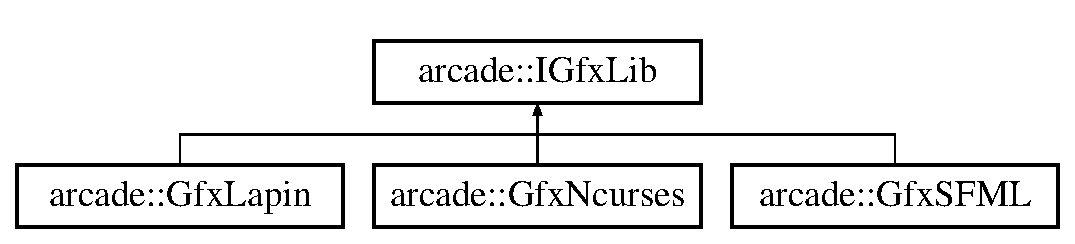
\includegraphics[height=2.000000cm]{classarcade_1_1_i_gfx_lib}
\end{center}
\end{figure}
\subsection*{Public Member Functions}
\begin{DoxyCompactItemize}
\item 
virtual \hyperlink{classarcade_1_1_i_gfx_lib_a1dc0971c862d69be60af1d3b82960c77}{$\sim$\+I\+Gfx\+Lib} ()
\begin{DoxyCompactList}\small\item\em Virtual destructor of the interface. \end{DoxyCompactList}\item 
virtual bool \hyperlink{classarcade_1_1_i_gfx_lib_a82cdd82f168ca898ef81edf82ca6147a}{poll\+Event} (\hyperlink{structarcade_1_1_event}{Event} \&e)=0
\begin{DoxyCompactList}\small\item\em Function to poll events from the graphic lib. \end{DoxyCompactList}\item 
virtual bool \hyperlink{classarcade_1_1_i_gfx_lib_a68cfbc987dfecca5b1405e36e00157b2}{does\+Support\+Sound} () const =0
\begin{DoxyCompactList}\small\item\em Ask if the library support sound. \end{DoxyCompactList}\item 
virtual void \hyperlink{classarcade_1_1_i_gfx_lib_a725faf0722d284d15eb389b0a1891a27}{load\+Sounds} (std\+::vector$<$ std\+::pair$<$ std\+::string, \hyperlink{namespacearcade_a3bb4743a2eea59f3927e404e6549cae5}{Sound\+Type} $>$ $>$ const \&sounds)=0
\begin{DoxyCompactList}\small\item\em Ask the lib to remove and load new sounds. \end{DoxyCompactList}\item 
virtual void \hyperlink{classarcade_1_1_i_gfx_lib_a0b965ed555739ef366b27583799d794c}{sound\+Control} (const \hyperlink{structarcade_1_1_sound}{Sound} \&sound)=0
\begin{DoxyCompactList}\small\item\em Ask the lib to play a sound. \end{DoxyCompactList}\item 
virtual void \hyperlink{classarcade_1_1_i_gfx_lib_ad5b301c8ff56c428971a2a006514b709}{load\+Sprites} (std\+::vector$<$ std\+::unique\+\_\+ptr$<$ \hyperlink{classarcade_1_1_i_sprite}{I\+Sprite} $>$$>$ \&\&sprites)=0
\begin{DoxyCompactList}\small\item\em Load sprites in the lib from the paths given by the game. \end{DoxyCompactList}\item 
virtual void \hyperlink{classarcade_1_1_i_gfx_lib_addc883f69b75e6ec4927027aad94f5b5}{update\+Map} (\hyperlink{classarcade_1_1_i_map}{I\+Map} const \&map)=0
\begin{DoxyCompactList}\small\item\em Update the map displayed. \end{DoxyCompactList}\item 
virtual void \hyperlink{classarcade_1_1_i_gfx_lib_ae3f443cc341512433815e8bf2dee3e0d}{update\+G\+UI} (\hyperlink{classarcade_1_1_i_g_u_i}{I\+G\+UI} \&gui)=0
\begin{DoxyCompactList}\small\item\em Update the \hyperlink{classarcade_1_1_g_u_i}{G\+UI} displayed. \end{DoxyCompactList}\item 
virtual void \hyperlink{classarcade_1_1_i_gfx_lib_a7f280525c718a44c1e05cfe0ba5304c3}{display} ()=0
\begin{DoxyCompactList}\small\item\em Display the map and \hyperlink{classarcade_1_1_g_u_i}{G\+UI}. \end{DoxyCompactList}\item 
virtual void \hyperlink{classarcade_1_1_i_gfx_lib_a4116b3d4f503c4a795539b584f77a73d}{clear} ()=0
\begin{DoxyCompactList}\small\item\em Ask the lib to clear the screen. \end{DoxyCompactList}\end{DoxyCompactItemize}


\subsection{Detailed Description}
Interface of a graphic lib for the \hyperlink{classarcade_1_1_core}{Core} program. 

This interface will be used by the \hyperlink{classarcade_1_1_core}{Core} program to manipulate a graphic lib without knowing any detail about it The \hyperlink{classarcade_1_1_core}{Core} will always do \char`\"{}request\char`\"{} to the lib, to get information or ask for displaying the map and \hyperlink{classarcade_1_1_g_u_i}{G\+UI}, for example. The \hyperlink{classarcade_1_1_i_gfx_lib}{I\+Gfx\+Lib} will never have a reference to the \hyperlink{classarcade_1_1_core}{Core}, or communicate directly with it. Never. Ever. 

\subsection{Constructor \& Destructor Documentation}
\mbox{\Hypertarget{classarcade_1_1_i_gfx_lib_a1dc0971c862d69be60af1d3b82960c77}\label{classarcade_1_1_i_gfx_lib_a1dc0971c862d69be60af1d3b82960c77}} 
\index{arcade\+::\+I\+Gfx\+Lib@{arcade\+::\+I\+Gfx\+Lib}!````~I\+Gfx\+Lib@{$\sim$\+I\+Gfx\+Lib}}
\index{````~I\+Gfx\+Lib@{$\sim$\+I\+Gfx\+Lib}!arcade\+::\+I\+Gfx\+Lib@{arcade\+::\+I\+Gfx\+Lib}}
\subsubsection{\texorpdfstring{$\sim$\+I\+Gfx\+Lib()}{~IGfxLib()}}
{\footnotesize\ttfamily arcade\+::\+I\+Gfx\+Lib\+::$\sim$\+I\+Gfx\+Lib (\begin{DoxyParamCaption}{ }\end{DoxyParamCaption})\hspace{0.3cm}{\ttfamily [inline]}, {\ttfamily [virtual]}}



Virtual destructor of the interface. 



\subsection{Member Function Documentation}
\mbox{\Hypertarget{classarcade_1_1_i_gfx_lib_a4116b3d4f503c4a795539b584f77a73d}\label{classarcade_1_1_i_gfx_lib_a4116b3d4f503c4a795539b584f77a73d}} 
\index{arcade\+::\+I\+Gfx\+Lib@{arcade\+::\+I\+Gfx\+Lib}!clear@{clear}}
\index{clear@{clear}!arcade\+::\+I\+Gfx\+Lib@{arcade\+::\+I\+Gfx\+Lib}}
\subsubsection{\texorpdfstring{clear()}{clear()}}
{\footnotesize\ttfamily void arcade\+::\+I\+Gfx\+Lib\+::clear (\begin{DoxyParamCaption}{ }\end{DoxyParamCaption})\hspace{0.3cm}{\ttfamily [pure virtual]}}



Ask the lib to clear the screen. 



Implemented in \hyperlink{classarcade_1_1_gfx_lapin_a42dd719cbf1cd88c3abf70d16f02fd92}{arcade\+::\+Gfx\+Lapin}, \hyperlink{classarcade_1_1_gfx_s_f_m_l_a12711203981dc2b9ce60df96d0aa6f55}{arcade\+::\+Gfx\+S\+F\+ML}, and \hyperlink{classarcade_1_1_gfx_ncurses_aaf443541674ace2e915e393156adf232}{arcade\+::\+Gfx\+Ncurses}.

\mbox{\Hypertarget{classarcade_1_1_i_gfx_lib_a7f280525c718a44c1e05cfe0ba5304c3}\label{classarcade_1_1_i_gfx_lib_a7f280525c718a44c1e05cfe0ba5304c3}} 
\index{arcade\+::\+I\+Gfx\+Lib@{arcade\+::\+I\+Gfx\+Lib}!display@{display}}
\index{display@{display}!arcade\+::\+I\+Gfx\+Lib@{arcade\+::\+I\+Gfx\+Lib}}
\subsubsection{\texorpdfstring{display()}{display()}}
{\footnotesize\ttfamily void arcade\+::\+I\+Gfx\+Lib\+::display (\begin{DoxyParamCaption}{ }\end{DoxyParamCaption})\hspace{0.3cm}{\ttfamily [pure virtual]}}



Display the map and \hyperlink{classarcade_1_1_g_u_i}{G\+UI}. 



Implemented in \hyperlink{classarcade_1_1_gfx_lapin_ac7c96886eb54a7d2f18e528e8f0c7ba1}{arcade\+::\+Gfx\+Lapin}, \hyperlink{classarcade_1_1_gfx_s_f_m_l_a590d6b932d5200a1367d8a2ff76def61}{arcade\+::\+Gfx\+S\+F\+ML}, and \hyperlink{classarcade_1_1_gfx_ncurses_aa119cdff68869bcd3829bb9fa9eaa373}{arcade\+::\+Gfx\+Ncurses}.

\mbox{\Hypertarget{classarcade_1_1_i_gfx_lib_a68cfbc987dfecca5b1405e36e00157b2}\label{classarcade_1_1_i_gfx_lib_a68cfbc987dfecca5b1405e36e00157b2}} 
\index{arcade\+::\+I\+Gfx\+Lib@{arcade\+::\+I\+Gfx\+Lib}!does\+Support\+Sound@{does\+Support\+Sound}}
\index{does\+Support\+Sound@{does\+Support\+Sound}!arcade\+::\+I\+Gfx\+Lib@{arcade\+::\+I\+Gfx\+Lib}}
\subsubsection{\texorpdfstring{does\+Support\+Sound()}{doesSupportSound()}}
{\footnotesize\ttfamily bool arcade\+::\+I\+Gfx\+Lib\+::does\+Support\+Sound (\begin{DoxyParamCaption}{ }\end{DoxyParamCaption}) const\hspace{0.3cm}{\ttfamily [pure virtual]}}



Ask if the library support sound. 



Implemented in \hyperlink{classarcade_1_1_gfx_s_f_m_l_aa8d0f997c7ddcb68526e0f19f5bad77d}{arcade\+::\+Gfx\+S\+F\+ML}, \hyperlink{classarcade_1_1_gfx_lapin_ae84337d3ae5e24a61f160d3ac99d4e10}{arcade\+::\+Gfx\+Lapin}, and \hyperlink{classarcade_1_1_gfx_ncurses_ab100f60173ccd55f19c30627ace55101}{arcade\+::\+Gfx\+Ncurses}.

\mbox{\Hypertarget{classarcade_1_1_i_gfx_lib_a725faf0722d284d15eb389b0a1891a27}\label{classarcade_1_1_i_gfx_lib_a725faf0722d284d15eb389b0a1891a27}} 
\index{arcade\+::\+I\+Gfx\+Lib@{arcade\+::\+I\+Gfx\+Lib}!load\+Sounds@{load\+Sounds}}
\index{load\+Sounds@{load\+Sounds}!arcade\+::\+I\+Gfx\+Lib@{arcade\+::\+I\+Gfx\+Lib}}
\subsubsection{\texorpdfstring{load\+Sounds()}{loadSounds()}}
{\footnotesize\ttfamily virtual void arcade\+::\+I\+Gfx\+Lib\+::load\+Sounds (\begin{DoxyParamCaption}\item[{std\+::vector$<$ std\+::pair$<$ std\+::string, \hyperlink{namespacearcade_a3bb4743a2eea59f3927e404e6549cae5}{Sound\+Type} $>$ $>$ const \&}]{sounds }\end{DoxyParamCaption})\hspace{0.3cm}{\ttfamily [pure virtual]}}



Ask the lib to remove and load new sounds. 



Implemented in \hyperlink{classarcade_1_1_gfx_s_f_m_l_aaec16dc42e480cdb6b6cbc3f75e4951c}{arcade\+::\+Gfx\+S\+F\+ML}, \hyperlink{classarcade_1_1_gfx_lapin_a54039353c2da52bb45b233d4b8839551}{arcade\+::\+Gfx\+Lapin}, and \hyperlink{classarcade_1_1_gfx_ncurses_a450bb0bdb3a31f8733cc71cb39ddfb16}{arcade\+::\+Gfx\+Ncurses}.

\mbox{\Hypertarget{classarcade_1_1_i_gfx_lib_ad5b301c8ff56c428971a2a006514b709}\label{classarcade_1_1_i_gfx_lib_ad5b301c8ff56c428971a2a006514b709}} 
\index{arcade\+::\+I\+Gfx\+Lib@{arcade\+::\+I\+Gfx\+Lib}!load\+Sprites@{load\+Sprites}}
\index{load\+Sprites@{load\+Sprites}!arcade\+::\+I\+Gfx\+Lib@{arcade\+::\+I\+Gfx\+Lib}}
\subsubsection{\texorpdfstring{load\+Sprites()}{loadSprites()}}
{\footnotesize\ttfamily std\+::vector$<$ int $>$ const  \& arcade\+::\+I\+Gfx\+Lib\+::load\+Sprites (\begin{DoxyParamCaption}\item[{std\+::vector$<$ std\+::unique\+\_\+ptr$<$ \hyperlink{classarcade_1_1_i_sprite}{I\+Sprite} $>$$>$ \&\&}]{sprites }\end{DoxyParamCaption})\hspace{0.3cm}{\ttfamily [pure virtual]}}



Load sprites in the lib from the paths given by the game. 


\begin{DoxyParams}{Parameters}
{\em sprites} & to pass the path of your sprites to give your lib the way to search your assets \\
\hline
\end{DoxyParams}


Implemented in \hyperlink{classarcade_1_1_gfx_s_f_m_l_a1e586ce151c47e3b5a6abcfdf5ecdc79}{arcade\+::\+Gfx\+S\+F\+ML}, \hyperlink{classarcade_1_1_gfx_lapin_a164a694063507041dbd78415898d5157}{arcade\+::\+Gfx\+Lapin}, and \hyperlink{classarcade_1_1_gfx_ncurses_a6a412ec8047964035f0d75e64fd8dc44}{arcade\+::\+Gfx\+Ncurses}.

\mbox{\Hypertarget{classarcade_1_1_i_gfx_lib_a82cdd82f168ca898ef81edf82ca6147a}\label{classarcade_1_1_i_gfx_lib_a82cdd82f168ca898ef81edf82ca6147a}} 
\index{arcade\+::\+I\+Gfx\+Lib@{arcade\+::\+I\+Gfx\+Lib}!poll\+Event@{poll\+Event}}
\index{poll\+Event@{poll\+Event}!arcade\+::\+I\+Gfx\+Lib@{arcade\+::\+I\+Gfx\+Lib}}
\subsubsection{\texorpdfstring{poll\+Event()}{pollEvent()}}
{\footnotesize\ttfamily bool arcade\+::\+I\+Gfx\+Lib\+::poll\+Event (\begin{DoxyParamCaption}\item[{\hyperlink{structarcade_1_1_event}{Event} \&}]{e }\end{DoxyParamCaption})\hspace{0.3cm}{\ttfamily [pure virtual]}}



Function to poll events from the graphic lib. 

If there is an event to poll, e is filled and true is returned. If not, false is returned. 

Implemented in \hyperlink{classarcade_1_1_gfx_s_f_m_l_a7c2d800770d4218eb38c8b01f5890aa3}{arcade\+::\+Gfx\+S\+F\+ML}, \hyperlink{classarcade_1_1_gfx_lapin_a80f4cae576f05ddc8ab94d5a348226c5}{arcade\+::\+Gfx\+Lapin}, and \hyperlink{classarcade_1_1_gfx_ncurses_aa16f7c823041b931025f750b4050318a}{arcade\+::\+Gfx\+Ncurses}.

\mbox{\Hypertarget{classarcade_1_1_i_gfx_lib_a0b965ed555739ef366b27583799d794c}\label{classarcade_1_1_i_gfx_lib_a0b965ed555739ef366b27583799d794c}} 
\index{arcade\+::\+I\+Gfx\+Lib@{arcade\+::\+I\+Gfx\+Lib}!sound\+Control@{sound\+Control}}
\index{sound\+Control@{sound\+Control}!arcade\+::\+I\+Gfx\+Lib@{arcade\+::\+I\+Gfx\+Lib}}
\subsubsection{\texorpdfstring{sound\+Control()}{soundControl()}}
{\footnotesize\ttfamily void arcade\+::\+I\+Gfx\+Lib\+::sound\+Control (\begin{DoxyParamCaption}\item[{const \hyperlink{structarcade_1_1_sound}{Sound} \&}]{sound }\end{DoxyParamCaption})\hspace{0.3cm}{\ttfamily [pure virtual]}}



Ask the lib to play a sound. 



Implemented in \hyperlink{classarcade_1_1_gfx_s_f_m_l_a785424b9463d487365c781bf91eda6a8}{arcade\+::\+Gfx\+S\+F\+ML}, \hyperlink{classarcade_1_1_gfx_lapin_ad0f1a1014b88cf7f51ea85ab99e0c87b}{arcade\+::\+Gfx\+Lapin}, and \hyperlink{classarcade_1_1_gfx_ncurses_a5eabfc85f5ae13bf0592dd21add9f301}{arcade\+::\+Gfx\+Ncurses}.

\mbox{\Hypertarget{classarcade_1_1_i_gfx_lib_ae3f443cc341512433815e8bf2dee3e0d}\label{classarcade_1_1_i_gfx_lib_ae3f443cc341512433815e8bf2dee3e0d}} 
\index{arcade\+::\+I\+Gfx\+Lib@{arcade\+::\+I\+Gfx\+Lib}!update\+G\+UI@{update\+G\+UI}}
\index{update\+G\+UI@{update\+G\+UI}!arcade\+::\+I\+Gfx\+Lib@{arcade\+::\+I\+Gfx\+Lib}}
\subsubsection{\texorpdfstring{update\+G\+U\+I()}{updateGUI()}}
{\footnotesize\ttfamily virtual void arcade\+::\+I\+Gfx\+Lib\+::update\+G\+UI (\begin{DoxyParamCaption}\item[{\hyperlink{classarcade_1_1_i_g_u_i}{I\+G\+UI} \&}]{gui }\end{DoxyParamCaption})\hspace{0.3cm}{\ttfamily [pure virtual]}}



Update the \hyperlink{classarcade_1_1_g_u_i}{G\+UI} displayed. 



Implemented in \hyperlink{classarcade_1_1_gfx_s_f_m_l_ad8ba0c70b00c4132010ceabc2246bb59}{arcade\+::\+Gfx\+S\+F\+ML}, \hyperlink{classarcade_1_1_gfx_lapin_a6b226d0278ba5d43e956eb28557124ef}{arcade\+::\+Gfx\+Lapin}, and \hyperlink{classarcade_1_1_gfx_ncurses_a00469b26c23ff57efdbb2f99dedbbb11}{arcade\+::\+Gfx\+Ncurses}.

\mbox{\Hypertarget{classarcade_1_1_i_gfx_lib_addc883f69b75e6ec4927027aad94f5b5}\label{classarcade_1_1_i_gfx_lib_addc883f69b75e6ec4927027aad94f5b5}} 
\index{arcade\+::\+I\+Gfx\+Lib@{arcade\+::\+I\+Gfx\+Lib}!update\+Map@{update\+Map}}
\index{update\+Map@{update\+Map}!arcade\+::\+I\+Gfx\+Lib@{arcade\+::\+I\+Gfx\+Lib}}
\subsubsection{\texorpdfstring{update\+Map()}{updateMap()}}
{\footnotesize\ttfamily void arcade\+::\+I\+Gfx\+Lib\+::update\+Map (\begin{DoxyParamCaption}\item[{\hyperlink{classarcade_1_1_i_map}{I\+Map} const \&}]{map }\end{DoxyParamCaption})\hspace{0.3cm}{\ttfamily [pure virtual]}}



Update the map displayed. 



Implemented in \hyperlink{classarcade_1_1_gfx_s_f_m_l_ad21d26a1e549e2da25da1c9f4155151c}{arcade\+::\+Gfx\+S\+F\+ML}, \hyperlink{classarcade_1_1_gfx_lapin_a06f4eb48bd1ea7749d81870211115a46}{arcade\+::\+Gfx\+Lapin}, and \hyperlink{classarcade_1_1_gfx_ncurses_a4e02400d983845ebe37f374f3dd82793}{arcade\+::\+Gfx\+Ncurses}.



The documentation for this class was generated from the following file\+:\begin{DoxyCompactItemize}
\item 
arcade\+Interfaces/\hyperlink{_i_gfx_lib_8hpp}{I\+Gfx\+Lib.\+hpp}\end{DoxyCompactItemize}

\hypertarget{classarcade_1_1_i_g_u_i}{}\section{arcade\+:\+:I\+G\+UI Class Reference}
\label{classarcade_1_1_i_g_u_i}\index{arcade\+::\+I\+G\+UI@{arcade\+::\+I\+G\+UI}}


Interface representing a \hyperlink{classarcade_1_1_g_u_i}{G\+UI}.  




{\ttfamily \#include $<$I\+G\+U\+I.\+hpp$>$}

Inheritance diagram for arcade\+:\+:I\+G\+UI\+:\begin{figure}[H]
\begin{center}
\leavevmode
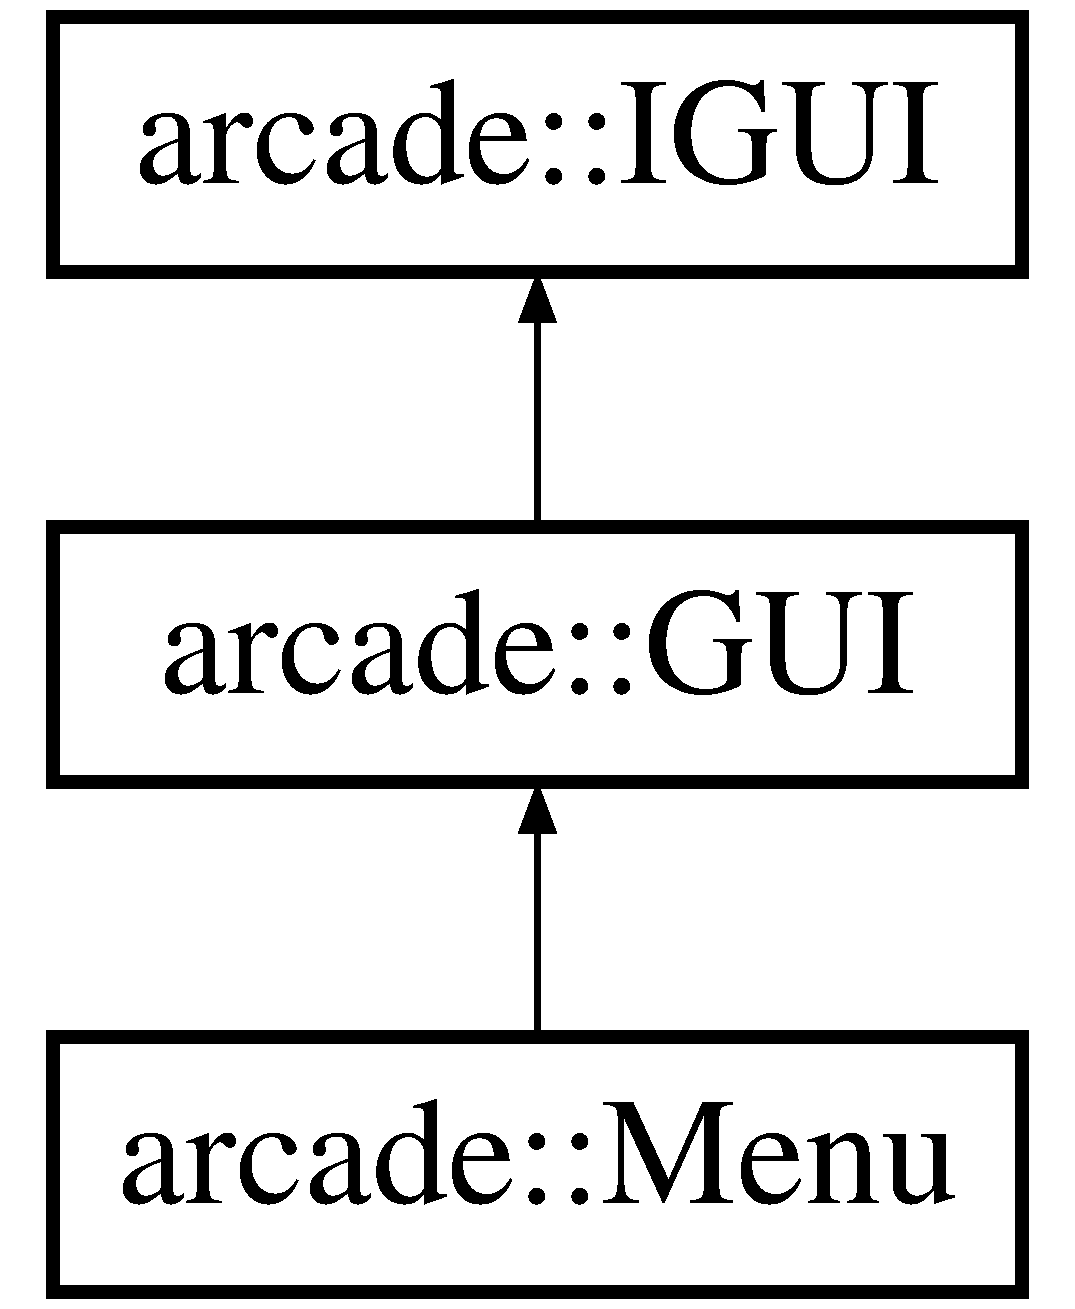
\includegraphics[height=3.000000cm]{classarcade_1_1_i_g_u_i}
\end{center}
\end{figure}
\subsection*{Public Member Functions}
\begin{DoxyCompactItemize}
\item 
virtual \hyperlink{classarcade_1_1_i_g_u_i_ae93e1b1b586b51ebfc760d35c0af3ba3}{$\sim$\+I\+G\+UI} ()
\begin{DoxyCompactList}\small\item\em Virtual destructor of the interface. \end{DoxyCompactList}\item 
virtual std\+::size\+\_\+t \hyperlink{classarcade_1_1_i_g_u_i_a5e9b36772c4affcc58243880e6d51d62}{size} () const =0
\begin{DoxyCompactList}\small\item\em Return the number of elements. \end{DoxyCompactList}\item 
virtual \hyperlink{classarcade_1_1_i_component}{I\+Component} \& \hyperlink{classarcade_1_1_i_g_u_i_aafde8788a75c98d0dfc1161e42e13558}{at} (std\+::size\+\_\+t n)=0
\begin{DoxyCompactList}\small\item\em Access to the n element. \end{DoxyCompactList}\end{DoxyCompactItemize}


\subsection{Detailed Description}
Interface representing a \hyperlink{classarcade_1_1_g_u_i}{G\+UI}. 

\subsection{Constructor \& Destructor Documentation}
\mbox{\Hypertarget{classarcade_1_1_i_g_u_i_ae93e1b1b586b51ebfc760d35c0af3ba3}\label{classarcade_1_1_i_g_u_i_ae93e1b1b586b51ebfc760d35c0af3ba3}} 
\index{arcade\+::\+I\+G\+UI@{arcade\+::\+I\+G\+UI}!````~I\+G\+UI@{$\sim$\+I\+G\+UI}}
\index{````~I\+G\+UI@{$\sim$\+I\+G\+UI}!arcade\+::\+I\+G\+UI@{arcade\+::\+I\+G\+UI}}
\subsubsection{\texorpdfstring{$\sim$\+I\+G\+U\+I()}{~IGUI()}}
{\footnotesize\ttfamily arcade\+::\+I\+G\+U\+I\+::$\sim$\+I\+G\+UI (\begin{DoxyParamCaption}{ }\end{DoxyParamCaption})\hspace{0.3cm}{\ttfamily [inline]}, {\ttfamily [virtual]}}



Virtual destructor of the interface. 



\subsection{Member Function Documentation}
\mbox{\Hypertarget{classarcade_1_1_i_g_u_i_aafde8788a75c98d0dfc1161e42e13558}\label{classarcade_1_1_i_g_u_i_aafde8788a75c98d0dfc1161e42e13558}} 
\index{arcade\+::\+I\+G\+UI@{arcade\+::\+I\+G\+UI}!at@{at}}
\index{at@{at}!arcade\+::\+I\+G\+UI@{arcade\+::\+I\+G\+UI}}
\subsubsection{\texorpdfstring{at()}{at()}}
{\footnotesize\ttfamily \hyperlink{classarcade_1_1_i_component}{I\+Component} \& arcade\+::\+I\+G\+U\+I\+::at (\begin{DoxyParamCaption}\item[{std\+::size\+\_\+t}]{n }\end{DoxyParamCaption})\hspace{0.3cm}{\ttfamily [pure virtual]}}



Access to the n element. 



Implemented in \hyperlink{classarcade_1_1_g_u_i_ab94910ea11fc43430227bfc716fd8c80}{arcade\+::\+G\+UI}.

\mbox{\Hypertarget{classarcade_1_1_i_g_u_i_a5e9b36772c4affcc58243880e6d51d62}\label{classarcade_1_1_i_g_u_i_a5e9b36772c4affcc58243880e6d51d62}} 
\index{arcade\+::\+I\+G\+UI@{arcade\+::\+I\+G\+UI}!size@{size}}
\index{size@{size}!arcade\+::\+I\+G\+UI@{arcade\+::\+I\+G\+UI}}
\subsubsection{\texorpdfstring{size()}{size()}}
{\footnotesize\ttfamily std\+::size\+\_\+t arcade\+::\+I\+G\+U\+I\+::size (\begin{DoxyParamCaption}{ }\end{DoxyParamCaption}) const\hspace{0.3cm}{\ttfamily [pure virtual]}}



Return the number of elements. 



Implemented in \hyperlink{classarcade_1_1_g_u_i_aa38b306ad674a221e0815cb600409598}{arcade\+::\+G\+UI}.



The documentation for this class was generated from the following file\+:\begin{DoxyCompactItemize}
\item 
arcade\+Interfaces/\hyperlink{_i_g_u_i_8hpp}{I\+G\+U\+I.\+hpp}\end{DoxyCompactItemize}

\hypertarget{classarcade_1_1_i_map}{}\section{arcade\+:\+:I\+Map Class Reference}
\label{classarcade_1_1_i_map}\index{arcade\+::\+I\+Map@{arcade\+::\+I\+Map}}


Interface representing a \hyperlink{classarcade_1_1_map}{Map}.  




{\ttfamily \#include $<$I\+Map.\+hpp$>$}

Inheritance diagram for arcade\+:\+:I\+Map\+:\begin{figure}[H]
\begin{center}
\leavevmode
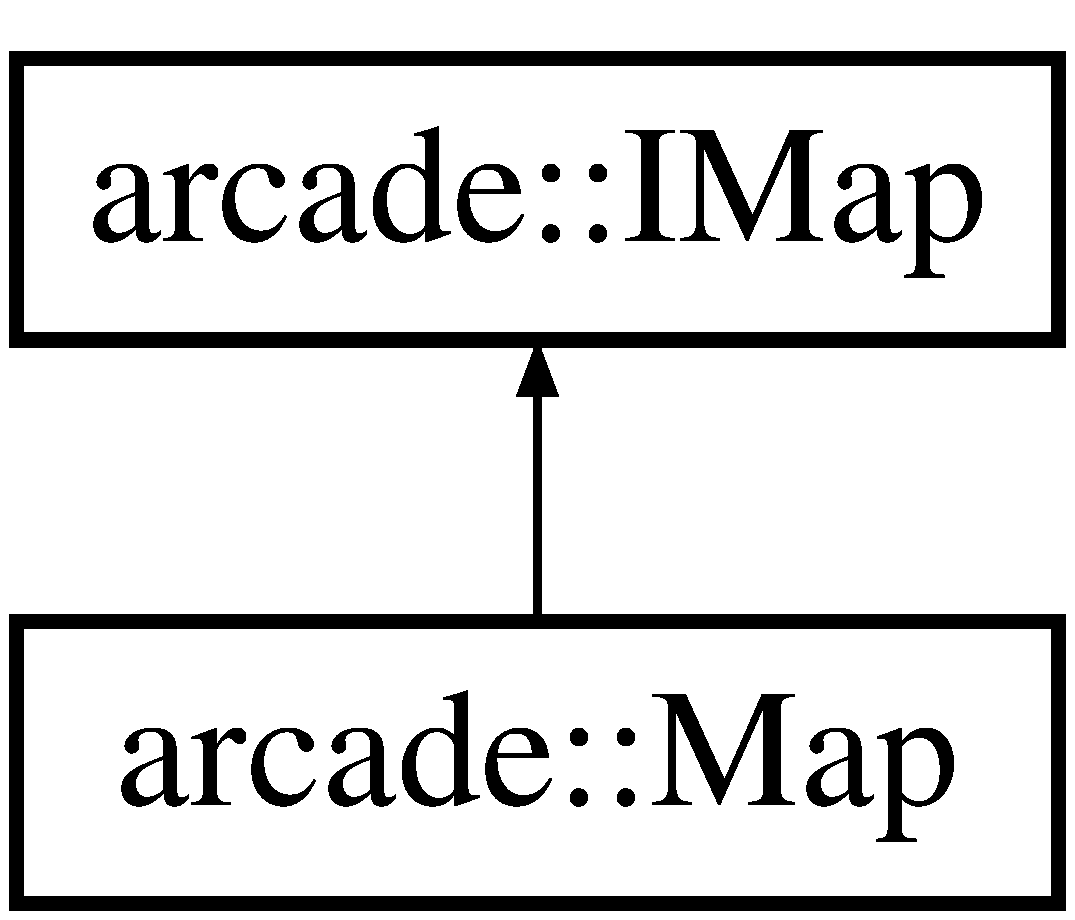
\includegraphics[height=2.000000cm]{classarcade_1_1_i_map}
\end{center}
\end{figure}
\subsection*{Public Member Functions}
\begin{DoxyCompactItemize}
\item 
virtual \hyperlink{classarcade_1_1_i_map_aaa3aa1b624552b9ab830067ab42f78dd}{$\sim$\+I\+Map} ()
\begin{DoxyCompactList}\small\item\em Virtual destructor of the interface. \end{DoxyCompactList}\item 
virtual size\+\_\+t \hyperlink{classarcade_1_1_i_map_a3e5fc4c5286f92fb49c8c7d0e79f4510}{get\+Layer\+Nb} () const =0
\begin{DoxyCompactList}\small\item\em Get the number of layers. \end{DoxyCompactList}\item 
virtual size\+\_\+t \hyperlink{classarcade_1_1_i_map_a6e7534eeff05277f1429037f8b01e25f}{get\+Width} () const =0
\begin{DoxyCompactList}\small\item\em Get the width of the map. \end{DoxyCompactList}\item 
virtual size\+\_\+t \hyperlink{classarcade_1_1_i_map_a9282ac731fa61b8c18241a309efbd6a0}{get\+Height} () const =0
\begin{DoxyCompactList}\small\item\em Get the height of the map. \end{DoxyCompactList}\item 
virtual \hyperlink{classarcade_1_1_i_tile}{I\+Tile} const  \& \hyperlink{classarcade_1_1_i_map_a8206c36a51d8394145fd3b7b29e42f8d}{at} (size\+\_\+t layer, size\+\_\+t \hyperlink{include_2_protocol_8hpp_a4dde988b1b2adba65ae3efa69f65d960}{x}, size\+\_\+t \hyperlink{include_2_protocol_8hpp_ab0580f504a7428539be299fa71565f30}{y}) const =0
\begin{DoxyCompactList}\small\item\em Get a specific \hyperlink{classarcade_1_1_i_tile}{I\+Tile} of the map. \end{DoxyCompactList}\end{DoxyCompactItemize}


\subsection{Detailed Description}
Interface representing a \hyperlink{classarcade_1_1_map}{Map}. 

A map is composed of layers, which contain tiles. Your \hyperlink{classarcade_1_1_map}{Map} must support them from its own If you want to access to the tile x\+:3 y\+:8 of the layer 2 you have to use the at method like I\+Map\+::at(2, 3, 8); 

\subsection{Constructor \& Destructor Documentation}
\mbox{\Hypertarget{classarcade_1_1_i_map_aaa3aa1b624552b9ab830067ab42f78dd}\label{classarcade_1_1_i_map_aaa3aa1b624552b9ab830067ab42f78dd}} 
\index{arcade\+::\+I\+Map@{arcade\+::\+I\+Map}!````~I\+Map@{$\sim$\+I\+Map}}
\index{````~I\+Map@{$\sim$\+I\+Map}!arcade\+::\+I\+Map@{arcade\+::\+I\+Map}}
\subsubsection{\texorpdfstring{$\sim$\+I\+Map()}{~IMap()}}
{\footnotesize\ttfamily arcade\+::\+I\+Map\+::$\sim$\+I\+Map (\begin{DoxyParamCaption}{ }\end{DoxyParamCaption})\hspace{0.3cm}{\ttfamily [inline]}, {\ttfamily [virtual]}}



Virtual destructor of the interface. 



\subsection{Member Function Documentation}
\mbox{\Hypertarget{classarcade_1_1_i_map_a8206c36a51d8394145fd3b7b29e42f8d}\label{classarcade_1_1_i_map_a8206c36a51d8394145fd3b7b29e42f8d}} 
\index{arcade\+::\+I\+Map@{arcade\+::\+I\+Map}!at@{at}}
\index{at@{at}!arcade\+::\+I\+Map@{arcade\+::\+I\+Map}}
\subsubsection{\texorpdfstring{at()}{at()}}
{\footnotesize\ttfamily \hyperlink{classarcade_1_1_i_tile}{I\+Tile} const  \& arcade\+::\+I\+Map\+::at (\begin{DoxyParamCaption}\item[{size\+\_\+t}]{layer,  }\item[{size\+\_\+t}]{x,  }\item[{size\+\_\+t}]{y }\end{DoxyParamCaption}) const\hspace{0.3cm}{\ttfamily [pure virtual]}}



Get a specific \hyperlink{classarcade_1_1_i_tile}{I\+Tile} of the map. 



Implemented in \hyperlink{classarcade_1_1_map_a8032d00c437cad8cedb646a0a1eb4bb1}{arcade\+::\+Map}.

\mbox{\Hypertarget{classarcade_1_1_i_map_a9282ac731fa61b8c18241a309efbd6a0}\label{classarcade_1_1_i_map_a9282ac731fa61b8c18241a309efbd6a0}} 
\index{arcade\+::\+I\+Map@{arcade\+::\+I\+Map}!get\+Height@{get\+Height}}
\index{get\+Height@{get\+Height}!arcade\+::\+I\+Map@{arcade\+::\+I\+Map}}
\subsubsection{\texorpdfstring{get\+Height()}{getHeight()}}
{\footnotesize\ttfamily size\+\_\+t arcade\+::\+I\+Map\+::get\+Height (\begin{DoxyParamCaption}{ }\end{DoxyParamCaption}) const\hspace{0.3cm}{\ttfamily [pure virtual]}}



Get the height of the map. 



Implemented in \hyperlink{classarcade_1_1_map_a914cc33687ccf159cc2876fc1d52657d}{arcade\+::\+Map}.

\mbox{\Hypertarget{classarcade_1_1_i_map_a3e5fc4c5286f92fb49c8c7d0e79f4510}\label{classarcade_1_1_i_map_a3e5fc4c5286f92fb49c8c7d0e79f4510}} 
\index{arcade\+::\+I\+Map@{arcade\+::\+I\+Map}!get\+Layer\+Nb@{get\+Layer\+Nb}}
\index{get\+Layer\+Nb@{get\+Layer\+Nb}!arcade\+::\+I\+Map@{arcade\+::\+I\+Map}}
\subsubsection{\texorpdfstring{get\+Layer\+Nb()}{getLayerNb()}}
{\footnotesize\ttfamily size\+\_\+t arcade\+::\+I\+Map\+::get\+Layer\+Nb (\begin{DoxyParamCaption}{ }\end{DoxyParamCaption}) const\hspace{0.3cm}{\ttfamily [pure virtual]}}



Get the number of layers. 



Implemented in \hyperlink{classarcade_1_1_map_a75d832d23939401ffe062b461839bc8d}{arcade\+::\+Map}.

\mbox{\Hypertarget{classarcade_1_1_i_map_a6e7534eeff05277f1429037f8b01e25f}\label{classarcade_1_1_i_map_a6e7534eeff05277f1429037f8b01e25f}} 
\index{arcade\+::\+I\+Map@{arcade\+::\+I\+Map}!get\+Width@{get\+Width}}
\index{get\+Width@{get\+Width}!arcade\+::\+I\+Map@{arcade\+::\+I\+Map}}
\subsubsection{\texorpdfstring{get\+Width()}{getWidth()}}
{\footnotesize\ttfamily size\+\_\+t arcade\+::\+I\+Map\+::get\+Width (\begin{DoxyParamCaption}{ }\end{DoxyParamCaption}) const\hspace{0.3cm}{\ttfamily [pure virtual]}}



Get the width of the map. 



Implemented in \hyperlink{classarcade_1_1_map_af48996ef9fc333a7c9ab6a9f2ddb7b56}{arcade\+::\+Map}.



The documentation for this class was generated from the following file\+:\begin{DoxyCompactItemize}
\item 
arcade\+Interfaces/\hyperlink{_i_map_8hpp}{I\+Map.\+hpp}\end{DoxyCompactItemize}

\hypertarget{classarcade_1_1_i_sprite}{}\section{arcade\+:\+:I\+Sprite Class Reference}
\label{classarcade_1_1_i_sprite}\index{arcade\+::\+I\+Sprite@{arcade\+::\+I\+Sprite}}


Interface to use in order to generate the sprite loading list.  




{\ttfamily \#include $<$I\+Sprite.\+hpp$>$}

Inheritance diagram for arcade\+:\+:I\+Sprite\+:\begin{figure}[H]
\begin{center}
\leavevmode
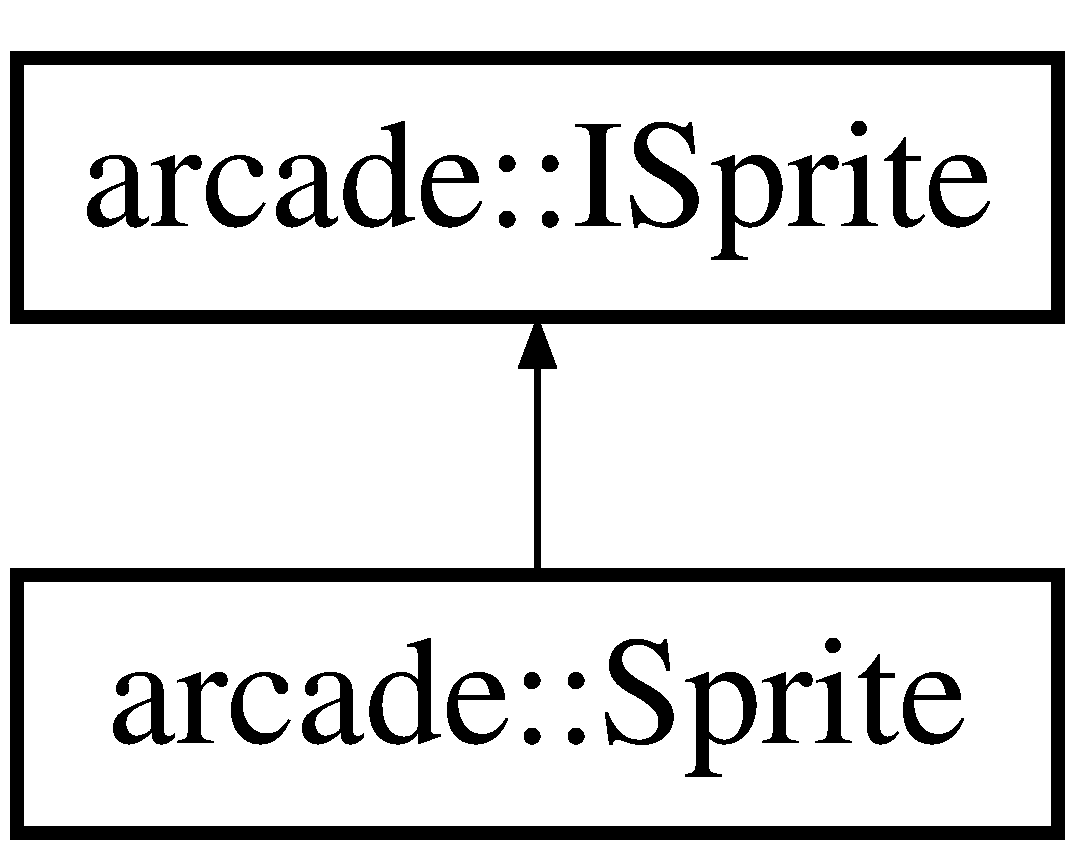
\includegraphics[height=2.000000cm]{classarcade_1_1_i_sprite}
\end{center}
\end{figure}
\subsection*{Public Member Functions}
\begin{DoxyCompactItemize}
\item 
virtual \hyperlink{classarcade_1_1_i_sprite_aa52abc5d79f3afa9ae82696d3bf9d3d3}{$\sim$\+I\+Sprite} ()
\begin{DoxyCompactList}\small\item\em virtual destructor \end{DoxyCompactList}\item 
virtual size\+\_\+t \hyperlink{classarcade_1_1_i_sprite_aa417a93a06968e42db16f8cbd2680c89}{sprites\+Count} () const =0
\begin{DoxyCompactList}\small\item\em returns the numbers of sprites \end{DoxyCompactList}\item 
virtual std\+::string \hyperlink{classarcade_1_1_i_sprite_ad47b6c128695746cd59e4b87435a7f09}{get\+Graphic\+Path} (size\+\_\+t pos) const =0
\begin{DoxyCompactList}\small\item\em generates on-\/the-\/fly the path to the sprite at position pos to load \end{DoxyCompactList}\item 
virtual char \hyperlink{classarcade_1_1_i_sprite_aa3ab1b0c35f865d38e82b6fb0abce20a}{get\+Ascii} (size\+\_\+t pos) const =0
\begin{DoxyCompactList}\small\item\em returns the ascii character at position pos from the animation sequence \end{DoxyCompactList}\end{DoxyCompactItemize}


\subsection{Detailed Description}
Interface to use in order to generate the sprite loading list. 

\subsection{Constructor \& Destructor Documentation}
\mbox{\Hypertarget{classarcade_1_1_i_sprite_aa52abc5d79f3afa9ae82696d3bf9d3d3}\label{classarcade_1_1_i_sprite_aa52abc5d79f3afa9ae82696d3bf9d3d3}} 
\index{arcade\+::\+I\+Sprite@{arcade\+::\+I\+Sprite}!````~I\+Sprite@{$\sim$\+I\+Sprite}}
\index{````~I\+Sprite@{$\sim$\+I\+Sprite}!arcade\+::\+I\+Sprite@{arcade\+::\+I\+Sprite}}
\subsubsection{\texorpdfstring{$\sim$\+I\+Sprite()}{~ISprite()}}
{\footnotesize\ttfamily arcade\+::\+I\+Sprite\+::$\sim$\+I\+Sprite (\begin{DoxyParamCaption}{ }\end{DoxyParamCaption})\hspace{0.3cm}{\ttfamily [inline]}, {\ttfamily [virtual]}}



virtual destructor 



\subsection{Member Function Documentation}
\mbox{\Hypertarget{classarcade_1_1_i_sprite_aa3ab1b0c35f865d38e82b6fb0abce20a}\label{classarcade_1_1_i_sprite_aa3ab1b0c35f865d38e82b6fb0abce20a}} 
\index{arcade\+::\+I\+Sprite@{arcade\+::\+I\+Sprite}!get\+Ascii@{get\+Ascii}}
\index{get\+Ascii@{get\+Ascii}!arcade\+::\+I\+Sprite@{arcade\+::\+I\+Sprite}}
\subsubsection{\texorpdfstring{get\+Ascii()}{getAscii()}}
{\footnotesize\ttfamily std\+::string const  \& arcade\+::\+I\+Sprite\+::get\+Ascii (\begin{DoxyParamCaption}\item[{size\+\_\+t}]{pos }\end{DoxyParamCaption}) const\hspace{0.3cm}{\ttfamily [pure virtual]}}



returns the ascii character at position pos from the animation sequence 



Implemented in \hyperlink{classarcade_1_1_sprite_a168a7f537e0fc6d2d4596cab449fde2c}{arcade\+::\+Sprite}.

\mbox{\Hypertarget{classarcade_1_1_i_sprite_ad47b6c128695746cd59e4b87435a7f09}\label{classarcade_1_1_i_sprite_ad47b6c128695746cd59e4b87435a7f09}} 
\index{arcade\+::\+I\+Sprite@{arcade\+::\+I\+Sprite}!get\+Graphic\+Path@{get\+Graphic\+Path}}
\index{get\+Graphic\+Path@{get\+Graphic\+Path}!arcade\+::\+I\+Sprite@{arcade\+::\+I\+Sprite}}
\subsubsection{\texorpdfstring{get\+Graphic\+Path()}{getGraphicPath()}}
{\footnotesize\ttfamily std\+::string arcade\+::\+I\+Sprite\+::get\+Graphic\+Path (\begin{DoxyParamCaption}\item[{size\+\_\+t}]{pos }\end{DoxyParamCaption}) const\hspace{0.3cm}{\ttfamily [pure virtual]}}



generates on-\/the-\/fly the path to the sprite at position pos to load 



Implemented in \hyperlink{classarcade_1_1_sprite_ad8f344724f99ad369c8c552274fface7}{arcade\+::\+Sprite}.

\mbox{\Hypertarget{classarcade_1_1_i_sprite_aa417a93a06968e42db16f8cbd2680c89}\label{classarcade_1_1_i_sprite_aa417a93a06968e42db16f8cbd2680c89}} 
\index{arcade\+::\+I\+Sprite@{arcade\+::\+I\+Sprite}!sprites\+Count@{sprites\+Count}}
\index{sprites\+Count@{sprites\+Count}!arcade\+::\+I\+Sprite@{arcade\+::\+I\+Sprite}}
\subsubsection{\texorpdfstring{sprites\+Count()}{spritesCount()}}
{\footnotesize\ttfamily size\+\_\+t arcade\+::\+I\+Sprite\+::sprites\+Count (\begin{DoxyParamCaption}{ }\end{DoxyParamCaption}) const\hspace{0.3cm}{\ttfamily [pure virtual]}}



returns the numbers of sprites 



Implemented in \hyperlink{classarcade_1_1_sprite_a99cc47358f32492ea89659b6b92f4d4c}{arcade\+::\+Sprite}.



The documentation for this class was generated from the following file\+:\begin{DoxyCompactItemize}
\item 
arcade\+Interfaces/\hyperlink{_i_sprite_8hpp}{I\+Sprite.\+hpp}\end{DoxyCompactItemize}

\hypertarget{classarcade_1_1_i_stat}{}\section{arcade\+:\+:I\+Stat Class Reference}
\label{classarcade_1_1_i_stat}\index{arcade\+::\+I\+Stat@{arcade\+::\+I\+Stat}}


Interface representing a player stat.  




{\ttfamily \#include $<$I\+Stat.\+hpp$>$}

\subsection*{Public Member Functions}
\begin{DoxyCompactItemize}
\item 
virtual \hyperlink{classarcade_1_1_i_stat_af8996c563dee5095d30592647fd0f00c}{$\sim$\+I\+Stat} ()
\begin{DoxyCompactList}\small\item\em Virtual destructor of the interface. \end{DoxyCompactList}\item 
virtual std\+::string const  \& \hyperlink{classarcade_1_1_i_stat_a6418289d2ae6b3d477ab8a9629487f18}{get\+Pseudo} () const =0
\begin{DoxyCompactList}\small\item\em Get the pseudo of the player. \end{DoxyCompactList}\item 
virtual long \hyperlink{classarcade_1_1_i_stat_acda674f38783f8d12db43103655642b7}{get\+Score} () const =0
\begin{DoxyCompactList}\small\item\em Get the player score. \end{DoxyCompactList}\end{DoxyCompactItemize}


\subsection{Detailed Description}
Interface representing a player stat. 

\subsection{Constructor \& Destructor Documentation}
\mbox{\Hypertarget{classarcade_1_1_i_stat_af8996c563dee5095d30592647fd0f00c}\label{classarcade_1_1_i_stat_af8996c563dee5095d30592647fd0f00c}} 
\index{arcade\+::\+I\+Stat@{arcade\+::\+I\+Stat}!````~I\+Stat@{$\sim$\+I\+Stat}}
\index{````~I\+Stat@{$\sim$\+I\+Stat}!arcade\+::\+I\+Stat@{arcade\+::\+I\+Stat}}
\subsubsection{\texorpdfstring{$\sim$\+I\+Stat()}{~IStat()}}
{\footnotesize\ttfamily arcade\+::\+I\+Stat\+::$\sim$\+I\+Stat (\begin{DoxyParamCaption}{ }\end{DoxyParamCaption})\hspace{0.3cm}{\ttfamily [inline]}, {\ttfamily [virtual]}}



Virtual destructor of the interface. 



\subsection{Member Function Documentation}
\mbox{\Hypertarget{classarcade_1_1_i_stat_a6418289d2ae6b3d477ab8a9629487f18}\label{classarcade_1_1_i_stat_a6418289d2ae6b3d477ab8a9629487f18}} 
\index{arcade\+::\+I\+Stat@{arcade\+::\+I\+Stat}!get\+Pseudo@{get\+Pseudo}}
\index{get\+Pseudo@{get\+Pseudo}!arcade\+::\+I\+Stat@{arcade\+::\+I\+Stat}}
\subsubsection{\texorpdfstring{get\+Pseudo()}{getPseudo()}}
{\footnotesize\ttfamily std\+::string const  \& arcade\+::\+I\+Stat\+::get\+Pseudo (\begin{DoxyParamCaption}{ }\end{DoxyParamCaption}) const\hspace{0.3cm}{\ttfamily [pure virtual]}}



Get the pseudo of the player. 

\mbox{\Hypertarget{classarcade_1_1_i_stat_acda674f38783f8d12db43103655642b7}\label{classarcade_1_1_i_stat_acda674f38783f8d12db43103655642b7}} 
\index{arcade\+::\+I\+Stat@{arcade\+::\+I\+Stat}!get\+Score@{get\+Score}}
\index{get\+Score@{get\+Score}!arcade\+::\+I\+Stat@{arcade\+::\+I\+Stat}}
\subsubsection{\texorpdfstring{get\+Score()}{getScore()}}
{\footnotesize\ttfamily long arcade\+::\+I\+Stat\+::get\+Score (\begin{DoxyParamCaption}{ }\end{DoxyParamCaption}) const\hspace{0.3cm}{\ttfamily [pure virtual]}}



Get the player score. 



The documentation for this class was generated from the following file\+:\begin{DoxyCompactItemize}
\item 
arcade\+Interfaces/\hyperlink{_i_stat_8hpp}{I\+Stat.\+hpp}\end{DoxyCompactItemize}

\hypertarget{classarcade_1_1_i_tile}{}\section{arcade\+:\+:I\+Tile Class Reference}
\label{classarcade_1_1_i_tile}\index{arcade\+::\+I\+Tile@{arcade\+::\+I\+Tile}}


Interface representing a tile.  




{\ttfamily \#include $<$I\+Tile.\+hpp$>$}

Inheritance diagram for arcade\+:\+:I\+Tile\+:\begin{figure}[H]
\begin{center}
\leavevmode
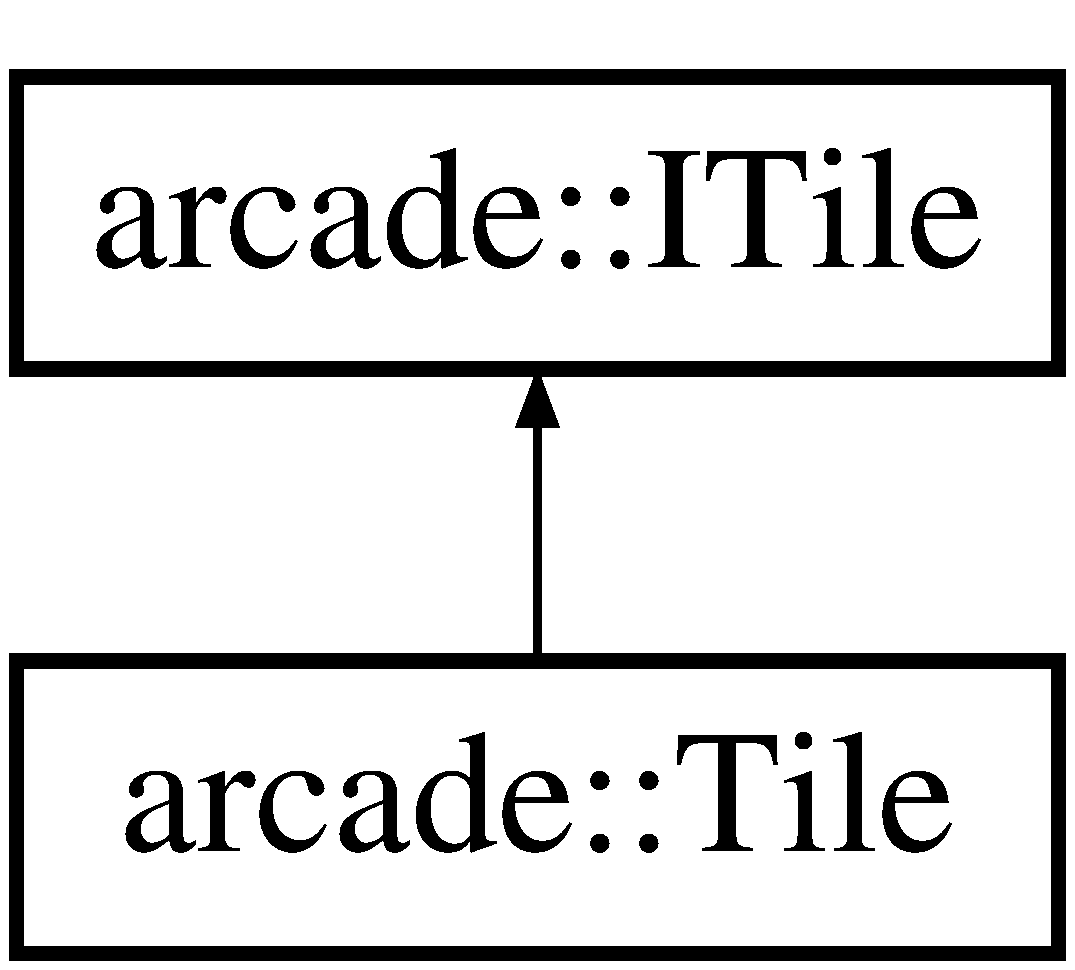
\includegraphics[height=2.000000cm]{classarcade_1_1_i_tile}
\end{center}
\end{figure}
\subsection*{Public Member Functions}
\begin{DoxyCompactItemize}
\item 
virtual \hyperlink{classarcade_1_1_i_tile_a45fb2120945fbddafb4b963d969a5b80}{$\sim$\+I\+Tile} ()
\begin{DoxyCompactList}\small\item\em Virtual destructor of the interface. \end{DoxyCompactList}\item 
virtual \hyperlink{unionarcade_1_1_color}{Color} \hyperlink{classarcade_1_1_i_tile_adb20cb553bc2ce17dc23125eb70b8329}{get\+Color} () const =0
\begin{DoxyCompactList}\small\item\em Get the color of the tile. \end{DoxyCompactList}\item 
virtual bool \hyperlink{classarcade_1_1_i_tile_ab2d6a5f8d4cfc6c606b8ad13d8dd88a4}{has\+Sprite} () const =0
\begin{DoxyCompactList}\small\item\em Returns if the \hyperlink{classarcade_1_1_tile}{Tile} has a sprite affected, if not, use \hyperlink{classarcade_1_1_i_tile_adb20cb553bc2ce17dc23125eb70b8329}{get\+Color()} \end{DoxyCompactList}\item 
virtual size\+\_\+t \hyperlink{classarcade_1_1_i_tile_a4c09e2ac12d75fe12e3d4d1ca4e08150}{get\+Sprite\+Id} () const =0
\begin{DoxyCompactList}\small\item\em Get the sprite ID (0 if none) \end{DoxyCompactList}\item 
virtual size\+\_\+t \hyperlink{classarcade_1_1_i_tile_a3e5cec4407ef6afb7e10d82fb1c93f5e}{get\+Sprite\+Pos} () const =0
\begin{DoxyCompactList}\small\item\em Get the sprite position in it\textquotesingle{}s animation. \end{DoxyCompactList}\item 
virtual double \hyperlink{classarcade_1_1_i_tile_aaa83bd96759c2c9f369be4b00b8a72d2}{get\+ShiftX} () const =0
\begin{DoxyCompactList}\small\item\em Get the tile position shift on x. \end{DoxyCompactList}\item 
virtual double \hyperlink{classarcade_1_1_i_tile_af7ca3cfb598eda00ac5b5f15f096e32f}{get\+ShiftY} () const =0
\begin{DoxyCompactList}\small\item\em Get the tile position shift on y. \end{DoxyCompactList}\end{DoxyCompactItemize}


\subsection{Detailed Description}
Interface representing a tile. 

A tile is a \char`\"{}block\char`\"{} of the map. It can be a wall, a empty block, a player, etc. It can be described with a type, a color and/or a sprite. 

\subsection{Constructor \& Destructor Documentation}
\mbox{\Hypertarget{classarcade_1_1_i_tile_a45fb2120945fbddafb4b963d969a5b80}\label{classarcade_1_1_i_tile_a45fb2120945fbddafb4b963d969a5b80}} 
\index{arcade\+::\+I\+Tile@{arcade\+::\+I\+Tile}!````~I\+Tile@{$\sim$\+I\+Tile}}
\index{````~I\+Tile@{$\sim$\+I\+Tile}!arcade\+::\+I\+Tile@{arcade\+::\+I\+Tile}}
\subsubsection{\texorpdfstring{$\sim$\+I\+Tile()}{~ITile()}}
{\footnotesize\ttfamily arcade\+::\+I\+Tile\+::$\sim$\+I\+Tile (\begin{DoxyParamCaption}{ }\end{DoxyParamCaption})\hspace{0.3cm}{\ttfamily [inline]}, {\ttfamily [virtual]}}



Virtual destructor of the interface. 



\subsection{Member Function Documentation}
\mbox{\Hypertarget{classarcade_1_1_i_tile_adb20cb553bc2ce17dc23125eb70b8329}\label{classarcade_1_1_i_tile_adb20cb553bc2ce17dc23125eb70b8329}} 
\index{arcade\+::\+I\+Tile@{arcade\+::\+I\+Tile}!get\+Color@{get\+Color}}
\index{get\+Color@{get\+Color}!arcade\+::\+I\+Tile@{arcade\+::\+I\+Tile}}
\subsubsection{\texorpdfstring{get\+Color()}{getColor()}}
{\footnotesize\ttfamily \hyperlink{unionarcade_1_1_color}{Color} arcade\+::\+I\+Tile\+::get\+Color (\begin{DoxyParamCaption}{ }\end{DoxyParamCaption}) const\hspace{0.3cm}{\ttfamily [pure virtual]}}



Get the color of the tile. 



Implemented in \hyperlink{classarcade_1_1_tile_a33f158dcb0b991ca565562a41ede70ba}{arcade\+::\+Tile}.

\mbox{\Hypertarget{classarcade_1_1_i_tile_aaa83bd96759c2c9f369be4b00b8a72d2}\label{classarcade_1_1_i_tile_aaa83bd96759c2c9f369be4b00b8a72d2}} 
\index{arcade\+::\+I\+Tile@{arcade\+::\+I\+Tile}!get\+ShiftX@{get\+ShiftX}}
\index{get\+ShiftX@{get\+ShiftX}!arcade\+::\+I\+Tile@{arcade\+::\+I\+Tile}}
\subsubsection{\texorpdfstring{get\+Shift\+X()}{getShiftX()}}
{\footnotesize\ttfamily double arcade\+::\+I\+Tile\+::get\+ShiftX (\begin{DoxyParamCaption}{ }\end{DoxyParamCaption}) const\hspace{0.3cm}{\ttfamily [pure virtual]}}



Get the tile position shift on x. 



Implemented in \hyperlink{classarcade_1_1_tile_a0db817dd3b7e0872e90d703bfea16005}{arcade\+::\+Tile}.

\mbox{\Hypertarget{classarcade_1_1_i_tile_af7ca3cfb598eda00ac5b5f15f096e32f}\label{classarcade_1_1_i_tile_af7ca3cfb598eda00ac5b5f15f096e32f}} 
\index{arcade\+::\+I\+Tile@{arcade\+::\+I\+Tile}!get\+ShiftY@{get\+ShiftY}}
\index{get\+ShiftY@{get\+ShiftY}!arcade\+::\+I\+Tile@{arcade\+::\+I\+Tile}}
\subsubsection{\texorpdfstring{get\+Shift\+Y()}{getShiftY()}}
{\footnotesize\ttfamily size\+\_\+t arcade\+::\+I\+Tile\+::get\+ShiftY (\begin{DoxyParamCaption}{ }\end{DoxyParamCaption}) const\hspace{0.3cm}{\ttfamily [pure virtual]}}



Get the tile position shift on y. 



Implemented in \hyperlink{classarcade_1_1_tile_aa28fe418563d90bd65e1c58510d28eef}{arcade\+::\+Tile}.

\mbox{\Hypertarget{classarcade_1_1_i_tile_a4c09e2ac12d75fe12e3d4d1ca4e08150}\label{classarcade_1_1_i_tile_a4c09e2ac12d75fe12e3d4d1ca4e08150}} 
\index{arcade\+::\+I\+Tile@{arcade\+::\+I\+Tile}!get\+Sprite\+Id@{get\+Sprite\+Id}}
\index{get\+Sprite\+Id@{get\+Sprite\+Id}!arcade\+::\+I\+Tile@{arcade\+::\+I\+Tile}}
\subsubsection{\texorpdfstring{get\+Sprite\+Id()}{getSpriteId()}}
{\footnotesize\ttfamily size\+\_\+t arcade\+::\+I\+Tile\+::get\+Sprite\+Id (\begin{DoxyParamCaption}{ }\end{DoxyParamCaption}) const\hspace{0.3cm}{\ttfamily [pure virtual]}}



Get the sprite ID (0 if none) 



Implemented in \hyperlink{classarcade_1_1_tile_afe2b3e7b4a6880b03772c240a2122d16}{arcade\+::\+Tile}.

\mbox{\Hypertarget{classarcade_1_1_i_tile_a3e5cec4407ef6afb7e10d82fb1c93f5e}\label{classarcade_1_1_i_tile_a3e5cec4407ef6afb7e10d82fb1c93f5e}} 
\index{arcade\+::\+I\+Tile@{arcade\+::\+I\+Tile}!get\+Sprite\+Pos@{get\+Sprite\+Pos}}
\index{get\+Sprite\+Pos@{get\+Sprite\+Pos}!arcade\+::\+I\+Tile@{arcade\+::\+I\+Tile}}
\subsubsection{\texorpdfstring{get\+Sprite\+Pos()}{getSpritePos()}}
{\footnotesize\ttfamily size\+\_\+t arcade\+::\+I\+Tile\+::get\+Sprite\+Pos (\begin{DoxyParamCaption}{ }\end{DoxyParamCaption}) const\hspace{0.3cm}{\ttfamily [pure virtual]}}



Get the sprite position in it\textquotesingle{}s animation. 



Implemented in \hyperlink{classarcade_1_1_tile_a0dfe91e5896b8cfc3afac522d901be0a}{arcade\+::\+Tile}.

\mbox{\Hypertarget{classarcade_1_1_i_tile_ab2d6a5f8d4cfc6c606b8ad13d8dd88a4}\label{classarcade_1_1_i_tile_ab2d6a5f8d4cfc6c606b8ad13d8dd88a4}} 
\index{arcade\+::\+I\+Tile@{arcade\+::\+I\+Tile}!has\+Sprite@{has\+Sprite}}
\index{has\+Sprite@{has\+Sprite}!arcade\+::\+I\+Tile@{arcade\+::\+I\+Tile}}
\subsubsection{\texorpdfstring{has\+Sprite()}{hasSprite()}}
{\footnotesize\ttfamily bool arcade\+::\+I\+Tile\+::has\+Sprite (\begin{DoxyParamCaption}{ }\end{DoxyParamCaption}) const\hspace{0.3cm}{\ttfamily [pure virtual]}}



Returns if the \hyperlink{classarcade_1_1_tile}{Tile} has a sprite affected, if not, use \hyperlink{classarcade_1_1_i_tile_adb20cb553bc2ce17dc23125eb70b8329}{get\+Color()} 



Implemented in \hyperlink{classarcade_1_1_tile_abb9bfea961e713a36213627d0787aae2}{arcade\+::\+Tile}.



The documentation for this class was generated from the following file\+:\begin{DoxyCompactItemize}
\item 
arcade\+Interfaces/\hyperlink{_i_tile_8hpp}{I\+Tile.\+hpp}\end{DoxyCompactItemize}

\hypertarget{unionkey}{}\section{key Union Reference}
\label{unionkey}\index{key@{key}}


Action of the event.  




{\ttfamily \#include $<$Event.\+hpp$>$}



\subsection{Detailed Description}
Action of the event. 

Key used (Keyboard, Mouse or Controller) 

The documentation for this union was generated from the following file\+:\begin{DoxyCompactItemize}
\item 
arcade\+Interfaces/\hyperlink{_event_8hpp}{Event.\+hpp}\end{DoxyCompactItemize}

\hypertarget{classarcade_1_1_layer}{}\section{arcade\+:\+:Layer Class Reference}
\label{classarcade_1_1_layer}\index{arcade\+::\+Layer@{arcade\+::\+Layer}}


{\ttfamily \#include $<$Layer.\+hpp$>$}

\subsection*{Public Member Functions}
\begin{DoxyCompactItemize}
\item 
virtual \hyperlink{classarcade_1_1_layer_ac24d42c242ff1c91282241f1d275828e}{$\sim$\+Layer} ()
\item 
\hyperlink{classarcade_1_1_layer_aca1a2c1f3ceff974a94e939fee334284}{Layer} (size\+\_\+t width, size\+\_\+t height)
\item 
std\+::vector$<$ std\+::unique\+\_\+ptr$<$ \hyperlink{classarcade_1_1_tile}{Tile} $>$ $>$ \& \hyperlink{classarcade_1_1_layer_a3d1c757621d4d14c7b4196c7ced76f5f}{operator\mbox{[}$\,$\mbox{]}} (int n)
\item 
std\+::vector$<$ std\+::unique\+\_\+ptr$<$ \hyperlink{classarcade_1_1_tile}{Tile} $>$ $>$ const  \& \hyperlink{classarcade_1_1_layer_a9067055ced1434f349f17767d77a9e6d}{operator\mbox{[}$\,$\mbox{]}} (int n) const
\item 
size\+\_\+t \hyperlink{classarcade_1_1_layer_a7af02d2e8135051c02897f27f83d09a5}{get\+Width} () const
\item 
size\+\_\+t \hyperlink{classarcade_1_1_layer_aa85bc4c2149a930c12ce17659de5e962}{get\+Height} () const
\end{DoxyCompactItemize}


\subsection{Constructor \& Destructor Documentation}
\mbox{\Hypertarget{classarcade_1_1_layer_ac24d42c242ff1c91282241f1d275828e}\label{classarcade_1_1_layer_ac24d42c242ff1c91282241f1d275828e}} 
\index{arcade\+::\+Layer@{arcade\+::\+Layer}!````~Layer@{$\sim$\+Layer}}
\index{````~Layer@{$\sim$\+Layer}!arcade\+::\+Layer@{arcade\+::\+Layer}}
\subsubsection{\texorpdfstring{$\sim$\+Layer()}{~Layer()}}
{\footnotesize\ttfamily arcade\+::\+Layer\+::$\sim$\+Layer (\begin{DoxyParamCaption}{ }\end{DoxyParamCaption})\hspace{0.3cm}{\ttfamily [virtual]}}

\mbox{\Hypertarget{classarcade_1_1_layer_aca1a2c1f3ceff974a94e939fee334284}\label{classarcade_1_1_layer_aca1a2c1f3ceff974a94e939fee334284}} 
\index{arcade\+::\+Layer@{arcade\+::\+Layer}!Layer@{Layer}}
\index{Layer@{Layer}!arcade\+::\+Layer@{arcade\+::\+Layer}}
\subsubsection{\texorpdfstring{Layer()}{Layer()}}
{\footnotesize\ttfamily arcade\+::\+Layer\+::\+Layer (\begin{DoxyParamCaption}\item[{size\+\_\+t}]{width,  }\item[{size\+\_\+t}]{height }\end{DoxyParamCaption})}



\subsection{Member Function Documentation}
\mbox{\Hypertarget{classarcade_1_1_layer_aa85bc4c2149a930c12ce17659de5e962}\label{classarcade_1_1_layer_aa85bc4c2149a930c12ce17659de5e962}} 
\index{arcade\+::\+Layer@{arcade\+::\+Layer}!get\+Height@{get\+Height}}
\index{get\+Height@{get\+Height}!arcade\+::\+Layer@{arcade\+::\+Layer}}
\subsubsection{\texorpdfstring{get\+Height()}{getHeight()}}
{\footnotesize\ttfamily size\+\_\+t arcade\+::\+Layer\+::get\+Height (\begin{DoxyParamCaption}{ }\end{DoxyParamCaption}) const}

\mbox{\Hypertarget{classarcade_1_1_layer_a7af02d2e8135051c02897f27f83d09a5}\label{classarcade_1_1_layer_a7af02d2e8135051c02897f27f83d09a5}} 
\index{arcade\+::\+Layer@{arcade\+::\+Layer}!get\+Width@{get\+Width}}
\index{get\+Width@{get\+Width}!arcade\+::\+Layer@{arcade\+::\+Layer}}
\subsubsection{\texorpdfstring{get\+Width()}{getWidth()}}
{\footnotesize\ttfamily size\+\_\+t arcade\+::\+Layer\+::get\+Width (\begin{DoxyParamCaption}{ }\end{DoxyParamCaption}) const}

\mbox{\Hypertarget{classarcade_1_1_layer_a3d1c757621d4d14c7b4196c7ced76f5f}\label{classarcade_1_1_layer_a3d1c757621d4d14c7b4196c7ced76f5f}} 
\index{arcade\+::\+Layer@{arcade\+::\+Layer}!operator\mbox{[}\mbox{]}@{operator[]}}
\index{operator\mbox{[}\mbox{]}@{operator[]}!arcade\+::\+Layer@{arcade\+::\+Layer}}
\subsubsection{\texorpdfstring{operator[]()}{operator[]()}\hspace{0.1cm}{\footnotesize\ttfamily [1/2]}}
{\footnotesize\ttfamily std\+::vector$<$ std\+::unique\+\_\+ptr$<$ \hyperlink{classarcade_1_1_tile}{arcade\+::\+Tile} $>$ $>$ \& arcade\+::\+Layer\+::operator\mbox{[}$\,$\mbox{]} (\begin{DoxyParamCaption}\item[{int}]{n }\end{DoxyParamCaption})}

\mbox{\Hypertarget{classarcade_1_1_layer_a9067055ced1434f349f17767d77a9e6d}\label{classarcade_1_1_layer_a9067055ced1434f349f17767d77a9e6d}} 
\index{arcade\+::\+Layer@{arcade\+::\+Layer}!operator\mbox{[}\mbox{]}@{operator[]}}
\index{operator\mbox{[}\mbox{]}@{operator[]}!arcade\+::\+Layer@{arcade\+::\+Layer}}
\subsubsection{\texorpdfstring{operator[]()}{operator[]()}\hspace{0.1cm}{\footnotesize\ttfamily [2/2]}}
{\footnotesize\ttfamily std\+::vector$<$ std\+::unique\+\_\+ptr$<$ \hyperlink{classarcade_1_1_tile}{arcade\+::\+Tile} $>$ $>$ const  \& arcade\+::\+Layer\+::operator\mbox{[}$\,$\mbox{]} (\begin{DoxyParamCaption}\item[{int}]{n }\end{DoxyParamCaption}) const}



The documentation for this class was generated from the following files\+:\begin{DoxyCompactItemize}
\item 
include/\hyperlink{_layer_8hpp}{Layer.\+hpp}\item 
srcs/\hyperlink{_layer_8cpp}{Layer.\+cpp}\end{DoxyCompactItemize}

\hypertarget{classarcade_1_1_map}{}\section{arcade\+:\+:Map Class Reference}
\label{classarcade_1_1_map}\index{arcade\+::\+Map@{arcade\+::\+Map}}


{\ttfamily \#include $<$Map.\+hpp$>$}

Inheritance diagram for arcade\+:\+:Map\+:\begin{figure}[H]
\begin{center}
\leavevmode
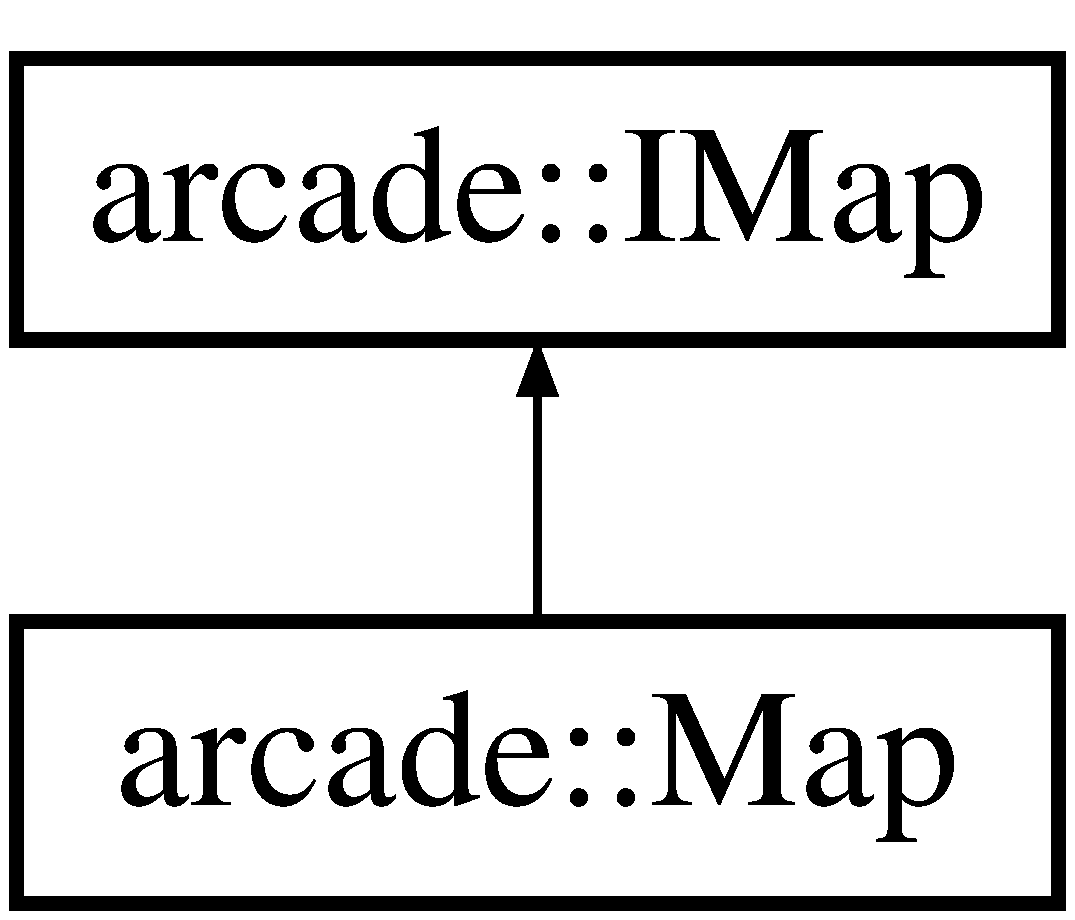
\includegraphics[height=2.000000cm]{classarcade_1_1_map}
\end{center}
\end{figure}
\subsection*{Public Member Functions}
\begin{DoxyCompactItemize}
\item 
virtual \hyperlink{classarcade_1_1_map_a5a07c82ff294b43e2091ad54f7a432f0}{$\sim$\+Map} ()
\item 
\hyperlink{classarcade_1_1_map_afc77786cf678dbf7fcf441889968ce13}{Map} (size\+\_\+t width, size\+\_\+t height, size\+\_\+t nb\+Layer)
\item 
\hyperlink{classarcade_1_1_layer}{Layer} \& \hyperlink{classarcade_1_1_map_afa393c5333d4cd1d24a1e145b4800769}{operator\mbox{[}$\,$\mbox{]}} (size\+\_\+t n)
\item 
const \hyperlink{classarcade_1_1_layer}{Layer} \& \hyperlink{classarcade_1_1_map_a83e8988805a8d8cd410080d342964c5f}{operator\mbox{[}$\,$\mbox{]}} (size\+\_\+t n) const
\item 
const \hyperlink{classarcade_1_1_i_tile}{I\+Tile} \& \hyperlink{classarcade_1_1_map_a8032d00c437cad8cedb646a0a1eb4bb1}{at} (size\+\_\+t layer, size\+\_\+t \hyperlink{include_2_protocol_8hpp_a4dde988b1b2adba65ae3efa69f65d960}{x}, size\+\_\+t \hyperlink{include_2_protocol_8hpp_ab0580f504a7428539be299fa71565f30}{y}) const override
\begin{DoxyCompactList}\small\item\em Get a specific \hyperlink{classarcade_1_1_i_tile}{I\+Tile} of the map. \end{DoxyCompactList}\item 
size\+\_\+t \hyperlink{classarcade_1_1_map_a75d832d23939401ffe062b461839bc8d}{get\+Layer\+Nb} () const override
\begin{DoxyCompactList}\small\item\em Get the number of layers. \end{DoxyCompactList}\item 
size\+\_\+t \hyperlink{classarcade_1_1_map_af48996ef9fc333a7c9ab6a9f2ddb7b56}{get\+Width} () const override
\begin{DoxyCompactList}\small\item\em Get the width of the map. \end{DoxyCompactList}\item 
size\+\_\+t \hyperlink{classarcade_1_1_map_a914cc33687ccf159cc2876fc1d52657d}{get\+Height} () const override
\begin{DoxyCompactList}\small\item\em Get the height of the map. \end{DoxyCompactList}\item 
bool \hyperlink{classarcade_1_1_map_a928573e629508a21455fdddf7298bcb4}{is\+Walkable} (size\+\_\+t layer\+\_\+idx, size\+\_\+t \hyperlink{include_2_protocol_8hpp_a4dde988b1b2adba65ae3efa69f65d960}{x}, size\+\_\+t \hyperlink{include_2_protocol_8hpp_ab0580f504a7428539be299fa71565f30}{y}) const
\item 
bool \hyperlink{classarcade_1_1_map_a15d5bbda533aab8362cac28a3f675d27}{is\+Walkable\+Offset} (size\+\_\+t layer\+\_\+idx, size\+\_\+t \hyperlink{include_2_protocol_8hpp_a4dde988b1b2adba65ae3efa69f65d960}{x}, size\+\_\+t \hyperlink{include_2_protocol_8hpp_ab0580f504a7428539be299fa71565f30}{y}, size\+\_\+t offset) const
\item 
void \hyperlink{classarcade_1_1_map_aafef74905482be652a9dc94f4b0c962e}{update\+Map\+Tile\+For\+Unit} (\hyperlink{classarcade_1_1_unit}{arcade\+::\+Unit} const \&unit, size\+\_\+t layer, \hyperlink{unionarcade_1_1_color}{Color} color, \hyperlink{namespacearcade_a61ba576694ea309cdf2b4b66902408ca}{Tile\+Type} tile\+Type, \hyperlink{namespacearcade_a2e0a64a64203f78c9efb84a1475a8cf4}{Tile\+Type\+Evolution} type\+Evolution, int sprite\+Id)
\end{DoxyCompactItemize}


\subsection{Constructor \& Destructor Documentation}
\mbox{\Hypertarget{classarcade_1_1_map_a5a07c82ff294b43e2091ad54f7a432f0}\label{classarcade_1_1_map_a5a07c82ff294b43e2091ad54f7a432f0}} 
\index{arcade\+::\+Map@{arcade\+::\+Map}!````~Map@{$\sim$\+Map}}
\index{````~Map@{$\sim$\+Map}!arcade\+::\+Map@{arcade\+::\+Map}}
\subsubsection{\texorpdfstring{$\sim$\+Map()}{~Map()}}
{\footnotesize\ttfamily arcade\+::\+Map\+::$\sim$\+Map (\begin{DoxyParamCaption}{ }\end{DoxyParamCaption})\hspace{0.3cm}{\ttfamily [virtual]}}

\mbox{\Hypertarget{classarcade_1_1_map_afc77786cf678dbf7fcf441889968ce13}\label{classarcade_1_1_map_afc77786cf678dbf7fcf441889968ce13}} 
\index{arcade\+::\+Map@{arcade\+::\+Map}!Map@{Map}}
\index{Map@{Map}!arcade\+::\+Map@{arcade\+::\+Map}}
\subsubsection{\texorpdfstring{Map()}{Map()}}
{\footnotesize\ttfamily arcade\+::\+Map\+::\+Map (\begin{DoxyParamCaption}\item[{size\+\_\+t}]{width,  }\item[{size\+\_\+t}]{height,  }\item[{size\+\_\+t}]{nb\+Layer }\end{DoxyParamCaption})}



\subsection{Member Function Documentation}
\mbox{\Hypertarget{classarcade_1_1_map_a8032d00c437cad8cedb646a0a1eb4bb1}\label{classarcade_1_1_map_a8032d00c437cad8cedb646a0a1eb4bb1}} 
\index{arcade\+::\+Map@{arcade\+::\+Map}!at@{at}}
\index{at@{at}!arcade\+::\+Map@{arcade\+::\+Map}}
\subsubsection{\texorpdfstring{at()}{at()}}
{\footnotesize\ttfamily const \hyperlink{classarcade_1_1_i_tile}{arcade\+::\+I\+Tile} \& arcade\+::\+Map\+::at (\begin{DoxyParamCaption}\item[{size\+\_\+t}]{layer,  }\item[{size\+\_\+t}]{x,  }\item[{size\+\_\+t}]{y }\end{DoxyParamCaption}) const\hspace{0.3cm}{\ttfamily [override]}, {\ttfamily [virtual]}}



Get a specific \hyperlink{classarcade_1_1_i_tile}{I\+Tile} of the map. 



Implements \hyperlink{classarcade_1_1_i_map_a8206c36a51d8394145fd3b7b29e42f8d}{arcade\+::\+I\+Map}.

\mbox{\Hypertarget{classarcade_1_1_map_a914cc33687ccf159cc2876fc1d52657d}\label{classarcade_1_1_map_a914cc33687ccf159cc2876fc1d52657d}} 
\index{arcade\+::\+Map@{arcade\+::\+Map}!get\+Height@{get\+Height}}
\index{get\+Height@{get\+Height}!arcade\+::\+Map@{arcade\+::\+Map}}
\subsubsection{\texorpdfstring{get\+Height()}{getHeight()}}
{\footnotesize\ttfamily size\+\_\+t arcade\+::\+Map\+::get\+Height (\begin{DoxyParamCaption}{ }\end{DoxyParamCaption}) const\hspace{0.3cm}{\ttfamily [override]}, {\ttfamily [virtual]}}



Get the height of the map. 



Implements \hyperlink{classarcade_1_1_i_map_a9282ac731fa61b8c18241a309efbd6a0}{arcade\+::\+I\+Map}.

\mbox{\Hypertarget{classarcade_1_1_map_a75d832d23939401ffe062b461839bc8d}\label{classarcade_1_1_map_a75d832d23939401ffe062b461839bc8d}} 
\index{arcade\+::\+Map@{arcade\+::\+Map}!get\+Layer\+Nb@{get\+Layer\+Nb}}
\index{get\+Layer\+Nb@{get\+Layer\+Nb}!arcade\+::\+Map@{arcade\+::\+Map}}
\subsubsection{\texorpdfstring{get\+Layer\+Nb()}{getLayerNb()}}
{\footnotesize\ttfamily size\+\_\+t arcade\+::\+Map\+::get\+Layer\+Nb (\begin{DoxyParamCaption}{ }\end{DoxyParamCaption}) const\hspace{0.3cm}{\ttfamily [override]}, {\ttfamily [virtual]}}



Get the number of layers. 



Implements \hyperlink{classarcade_1_1_i_map_a3e5fc4c5286f92fb49c8c7d0e79f4510}{arcade\+::\+I\+Map}.

\mbox{\Hypertarget{classarcade_1_1_map_af48996ef9fc333a7c9ab6a9f2ddb7b56}\label{classarcade_1_1_map_af48996ef9fc333a7c9ab6a9f2ddb7b56}} 
\index{arcade\+::\+Map@{arcade\+::\+Map}!get\+Width@{get\+Width}}
\index{get\+Width@{get\+Width}!arcade\+::\+Map@{arcade\+::\+Map}}
\subsubsection{\texorpdfstring{get\+Width()}{getWidth()}}
{\footnotesize\ttfamily size\+\_\+t arcade\+::\+Map\+::get\+Width (\begin{DoxyParamCaption}{ }\end{DoxyParamCaption}) const\hspace{0.3cm}{\ttfamily [override]}, {\ttfamily [virtual]}}



Get the width of the map. 



Implements \hyperlink{classarcade_1_1_i_map_a6e7534eeff05277f1429037f8b01e25f}{arcade\+::\+I\+Map}.

\mbox{\Hypertarget{classarcade_1_1_map_a928573e629508a21455fdddf7298bcb4}\label{classarcade_1_1_map_a928573e629508a21455fdddf7298bcb4}} 
\index{arcade\+::\+Map@{arcade\+::\+Map}!is\+Walkable@{is\+Walkable}}
\index{is\+Walkable@{is\+Walkable}!arcade\+::\+Map@{arcade\+::\+Map}}
\subsubsection{\texorpdfstring{is\+Walkable()}{isWalkable()}}
{\footnotesize\ttfamily bool arcade\+::\+Map\+::is\+Walkable (\begin{DoxyParamCaption}\item[{size\+\_\+t}]{layer\+\_\+idx,  }\item[{size\+\_\+t}]{x,  }\item[{size\+\_\+t}]{y }\end{DoxyParamCaption}) const}

\mbox{\Hypertarget{classarcade_1_1_map_a15d5bbda533aab8362cac28a3f675d27}\label{classarcade_1_1_map_a15d5bbda533aab8362cac28a3f675d27}} 
\index{arcade\+::\+Map@{arcade\+::\+Map}!is\+Walkable\+Offset@{is\+Walkable\+Offset}}
\index{is\+Walkable\+Offset@{is\+Walkable\+Offset}!arcade\+::\+Map@{arcade\+::\+Map}}
\subsubsection{\texorpdfstring{is\+Walkable\+Offset()}{isWalkableOffset()}}
{\footnotesize\ttfamily bool arcade\+::\+Map\+::is\+Walkable\+Offset (\begin{DoxyParamCaption}\item[{size\+\_\+t}]{layer\+\_\+idx,  }\item[{size\+\_\+t}]{x,  }\item[{size\+\_\+t}]{y,  }\item[{size\+\_\+t}]{offset }\end{DoxyParamCaption}) const}

\mbox{\Hypertarget{classarcade_1_1_map_afa393c5333d4cd1d24a1e145b4800769}\label{classarcade_1_1_map_afa393c5333d4cd1d24a1e145b4800769}} 
\index{arcade\+::\+Map@{arcade\+::\+Map}!operator\mbox{[}\mbox{]}@{operator[]}}
\index{operator\mbox{[}\mbox{]}@{operator[]}!arcade\+::\+Map@{arcade\+::\+Map}}
\subsubsection{\texorpdfstring{operator[]()}{operator[]()}\hspace{0.1cm}{\footnotesize\ttfamily [1/2]}}
{\footnotesize\ttfamily \hyperlink{classarcade_1_1_layer}{arcade\+::\+Layer} \& arcade\+::\+Map\+::operator\mbox{[}$\,$\mbox{]} (\begin{DoxyParamCaption}\item[{size\+\_\+t}]{n }\end{DoxyParamCaption})}

\mbox{\Hypertarget{classarcade_1_1_map_a83e8988805a8d8cd410080d342964c5f}\label{classarcade_1_1_map_a83e8988805a8d8cd410080d342964c5f}} 
\index{arcade\+::\+Map@{arcade\+::\+Map}!operator\mbox{[}\mbox{]}@{operator[]}}
\index{operator\mbox{[}\mbox{]}@{operator[]}!arcade\+::\+Map@{arcade\+::\+Map}}
\subsubsection{\texorpdfstring{operator[]()}{operator[]()}\hspace{0.1cm}{\footnotesize\ttfamily [2/2]}}
{\footnotesize\ttfamily const \hyperlink{classarcade_1_1_layer}{arcade\+::\+Layer} \& arcade\+::\+Map\+::operator\mbox{[}$\,$\mbox{]} (\begin{DoxyParamCaption}\item[{size\+\_\+t}]{n }\end{DoxyParamCaption}) const}

\mbox{\Hypertarget{classarcade_1_1_map_aafef74905482be652a9dc94f4b0c962e}\label{classarcade_1_1_map_aafef74905482be652a9dc94f4b0c962e}} 
\index{arcade\+::\+Map@{arcade\+::\+Map}!update\+Map\+Tile\+For\+Unit@{update\+Map\+Tile\+For\+Unit}}
\index{update\+Map\+Tile\+For\+Unit@{update\+Map\+Tile\+For\+Unit}!arcade\+::\+Map@{arcade\+::\+Map}}
\subsubsection{\texorpdfstring{update\+Map\+Tile\+For\+Unit()}{updateMapTileForUnit()}}
{\footnotesize\ttfamily void arcade\+::\+Map\+::update\+Map\+Tile\+For\+Unit (\begin{DoxyParamCaption}\item[{\hyperlink{classarcade_1_1_unit}{arcade\+::\+Unit} const \&}]{unit,  }\item[{size\+\_\+t}]{layer,  }\item[{\hyperlink{unionarcade_1_1_color}{Color}}]{color,  }\item[{\hyperlink{namespacearcade_a61ba576694ea309cdf2b4b66902408ca}{Tile\+Type}}]{tile\+Type,  }\item[{\hyperlink{namespacearcade_a2e0a64a64203f78c9efb84a1475a8cf4}{Tile\+Type\+Evolution}}]{type\+Evolution,  }\item[{int}]{sprite\+Id }\end{DoxyParamCaption})}



The documentation for this class was generated from the following files\+:\begin{DoxyCompactItemize}
\item 
include/\hyperlink{_map_8hpp}{Map.\+hpp}\item 
srcs/\hyperlink{_map_8cpp}{Map.\+cpp}\end{DoxyCompactItemize}

\hypertarget{classarcade_1_1_menu}{}\section{arcade\+:\+:Menu Class Reference}
\label{classarcade_1_1_menu}\index{arcade\+::\+Menu@{arcade\+::\+Menu}}


{\ttfamily \#include $<$Menu.\+hpp$>$}

Inheritance diagram for arcade\+:\+:Menu\+:\begin{figure}[H]
\begin{center}
\leavevmode
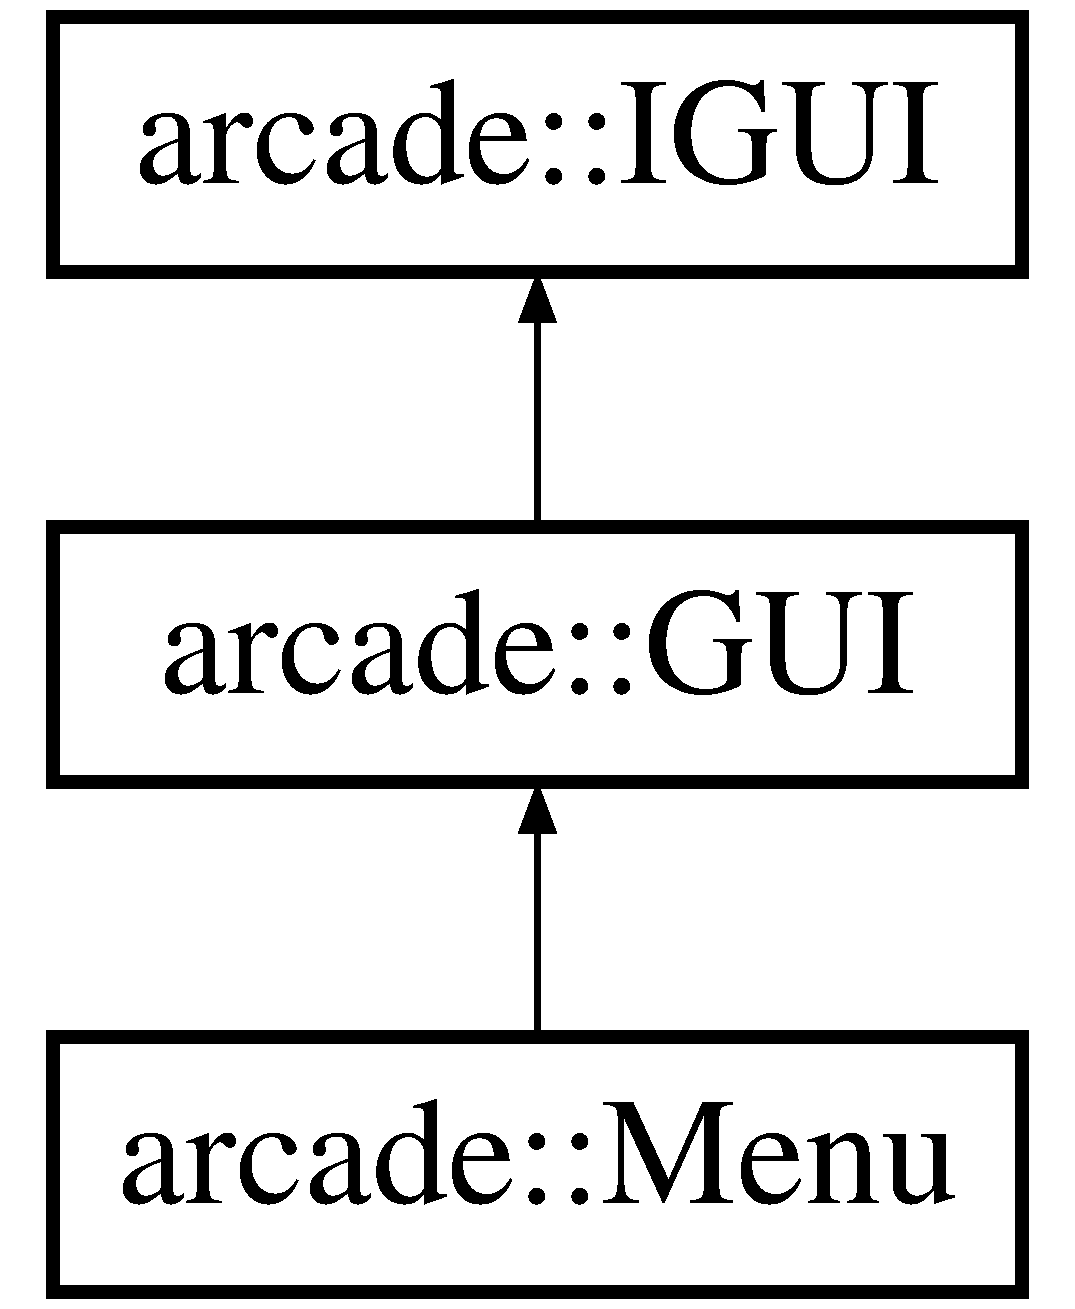
\includegraphics[height=3.000000cm]{classarcade_1_1_menu}
\end{center}
\end{figure}
\subsection*{Public Member Functions}
\begin{DoxyCompactItemize}
\item 
virtual \hyperlink{classarcade_1_1_menu_a2010367feb73b005d247f74fa0563d72}{$\sim$\+Menu} ()
\item 
\hyperlink{classarcade_1_1_menu_a1dab304f5e07c98f6527a0dac57db46b}{Menu} ()
\item 
\hyperlink{classarcade_1_1_menu_ab94e3c0b8e8db84a50e9748c02f648ce}{Menu} (std\+::vector$<$ std\+::string $>$ games\+Path, std\+::vector$<$ std\+::string $>$ gfx\+Path, size\+\_\+t gfx\+Id)
\item 
void \hyperlink{classarcade_1_1_menu_a1a18e92410e231d70277606f5c8bd4e9}{move\+Menu} (int menu, size\+\_\+t component)
\item 
void \hyperlink{classarcade_1_1_menu_a63906aaba91a3be7b0f4f8dcc46e87f4}{update\+Components} () override
\end{DoxyCompactItemize}
\subsection*{Additional Inherited Members}


\subsection{Constructor \& Destructor Documentation}
\mbox{\Hypertarget{classarcade_1_1_menu_a2010367feb73b005d247f74fa0563d72}\label{classarcade_1_1_menu_a2010367feb73b005d247f74fa0563d72}} 
\index{arcade\+::\+Menu@{arcade\+::\+Menu}!````~Menu@{$\sim$\+Menu}}
\index{````~Menu@{$\sim$\+Menu}!arcade\+::\+Menu@{arcade\+::\+Menu}}
\subsubsection{\texorpdfstring{$\sim$\+Menu()}{~Menu()}}
{\footnotesize\ttfamily arcade\+::\+Menu\+::$\sim$\+Menu (\begin{DoxyParamCaption}{ }\end{DoxyParamCaption})\hspace{0.3cm}{\ttfamily [virtual]}}

\mbox{\Hypertarget{classarcade_1_1_menu_a1dab304f5e07c98f6527a0dac57db46b}\label{classarcade_1_1_menu_a1dab304f5e07c98f6527a0dac57db46b}} 
\index{arcade\+::\+Menu@{arcade\+::\+Menu}!Menu@{Menu}}
\index{Menu@{Menu}!arcade\+::\+Menu@{arcade\+::\+Menu}}
\subsubsection{\texorpdfstring{Menu()}{Menu()}\hspace{0.1cm}{\footnotesize\ttfamily [1/2]}}
{\footnotesize\ttfamily arcade\+::\+Menu\+::\+Menu (\begin{DoxyParamCaption}{ }\end{DoxyParamCaption})}

\mbox{\Hypertarget{classarcade_1_1_menu_ab94e3c0b8e8db84a50e9748c02f648ce}\label{classarcade_1_1_menu_ab94e3c0b8e8db84a50e9748c02f648ce}} 
\index{arcade\+::\+Menu@{arcade\+::\+Menu}!Menu@{Menu}}
\index{Menu@{Menu}!arcade\+::\+Menu@{arcade\+::\+Menu}}
\subsubsection{\texorpdfstring{Menu()}{Menu()}\hspace{0.1cm}{\footnotesize\ttfamily [2/2]}}
{\footnotesize\ttfamily arcade\+::\+Menu\+::\+Menu (\begin{DoxyParamCaption}\item[{std\+::vector$<$ std\+::string $>$}]{games\+Path,  }\item[{std\+::vector$<$ std\+::string $>$}]{gfx\+Path,  }\item[{size\+\_\+t}]{gfx\+Id }\end{DoxyParamCaption})}



\subsection{Member Function Documentation}
\mbox{\Hypertarget{classarcade_1_1_menu_a1a18e92410e231d70277606f5c8bd4e9}\label{classarcade_1_1_menu_a1a18e92410e231d70277606f5c8bd4e9}} 
\index{arcade\+::\+Menu@{arcade\+::\+Menu}!move\+Menu@{move\+Menu}}
\index{move\+Menu@{move\+Menu}!arcade\+::\+Menu@{arcade\+::\+Menu}}
\subsubsection{\texorpdfstring{move\+Menu()}{moveMenu()}}
{\footnotesize\ttfamily void arcade\+::\+Menu\+::move\+Menu (\begin{DoxyParamCaption}\item[{int}]{menu,  }\item[{size\+\_\+t}]{component }\end{DoxyParamCaption})}

\mbox{\Hypertarget{classarcade_1_1_menu_a63906aaba91a3be7b0f4f8dcc46e87f4}\label{classarcade_1_1_menu_a63906aaba91a3be7b0f4f8dcc46e87f4}} 
\index{arcade\+::\+Menu@{arcade\+::\+Menu}!update\+Components@{update\+Components}}
\index{update\+Components@{update\+Components}!arcade\+::\+Menu@{arcade\+::\+Menu}}
\subsubsection{\texorpdfstring{update\+Components()}{updateComponents()}}
{\footnotesize\ttfamily void arcade\+::\+Menu\+::update\+Components (\begin{DoxyParamCaption}{ }\end{DoxyParamCaption})\hspace{0.3cm}{\ttfamily [override]}, {\ttfamily [virtual]}}



Reimplemented from \hyperlink{classarcade_1_1_g_u_i_abdf6ff80e7176b8a0e9c4561c5bfbf10}{arcade\+::\+G\+UI}.



The documentation for this class was generated from the following files\+:\begin{DoxyCompactItemize}
\item 
include/\hyperlink{_menu_8hpp}{Menu.\+hpp}\item 
srcs/\hyperlink{_menu_8cpp}{Menu.\+cpp}\end{DoxyCompactItemize}

\hypertarget{structarcade_1_1_mouse_pos}{}\section{arcade\+:\+:Mouse\+Pos Struct Reference}
\label{structarcade_1_1_mouse_pos}\index{arcade\+::\+Mouse\+Pos@{arcade\+::\+Mouse\+Pos}}


Mouse position (on the scale map)  




{\ttfamily \#include $<$Event.\+hpp$>$}

\subsection*{Public Attributes}
\begin{DoxyCompactItemize}
\item 
double \hyperlink{structarcade_1_1_mouse_pos_a0baa5eab2ede9028abdfa46dfbf3b901}{x}
\item 
double \hyperlink{structarcade_1_1_mouse_pos_a6737b813beae9a70aa6f7cbfc90154a6}{y}
\begin{DoxyCompactList}\small\item\em \hyperlink{structarcade_1_1_position}{Position} on x axis (horizontal) \end{DoxyCompactList}\end{DoxyCompactItemize}


\subsection{Detailed Description}
Mouse position (on the scale map) 

The position is not in pixel, but in \char`\"{}\+Tile\char`\"{} 

\subsection{Member Data Documentation}
\mbox{\Hypertarget{structarcade_1_1_mouse_pos_a0baa5eab2ede9028abdfa46dfbf3b901}\label{structarcade_1_1_mouse_pos_a0baa5eab2ede9028abdfa46dfbf3b901}} 
\index{arcade\+::\+Mouse\+Pos@{arcade\+::\+Mouse\+Pos}!x@{x}}
\index{x@{x}!arcade\+::\+Mouse\+Pos@{arcade\+::\+Mouse\+Pos}}
\subsubsection{\texorpdfstring{x}{x}}
{\footnotesize\ttfamily double arcade\+::\+Mouse\+Pos\+::x}

\mbox{\Hypertarget{structarcade_1_1_mouse_pos_a6737b813beae9a70aa6f7cbfc90154a6}\label{structarcade_1_1_mouse_pos_a6737b813beae9a70aa6f7cbfc90154a6}} 
\index{arcade\+::\+Mouse\+Pos@{arcade\+::\+Mouse\+Pos}!y@{y}}
\index{y@{y}!arcade\+::\+Mouse\+Pos@{arcade\+::\+Mouse\+Pos}}
\subsubsection{\texorpdfstring{y}{y}}
{\footnotesize\ttfamily double arcade\+::\+Mouse\+Pos\+::y}



\hyperlink{structarcade_1_1_position}{Position} on x axis (horizontal) 



The documentation for this struct was generated from the following file\+:\begin{DoxyCompactItemize}
\item 
arcade\+Interfaces/\hyperlink{_event_8hpp}{Event.\+hpp}\end{DoxyCompactItemize}

\hypertarget{structarcade_1_1_network_packet}{}\section{arcade\+:\+:Network\+Packet Struct Reference}
\label{structarcade_1_1_network_packet}\index{arcade\+::\+Network\+Packet@{arcade\+::\+Network\+Packet}}


Network packet.  




{\ttfamily \#include $<$Network\+Packet.\+hpp$>$}

\subsection*{Public Attributes}
\begin{DoxyCompactItemize}
\item 
\hyperlink{structarcade_1_1_network_packet_header}{Network\+Packet\+Header} \hyperlink{structarcade_1_1_network_packet_ad857cd0a4f6387035f4f954ca6d33676}{header}
\item 
uint32\+\_\+t \hyperlink{structarcade_1_1_network_packet_a1f6c07b81a4e7a276d933f326baae6fa}{len}
\item 
uint8\+\_\+t $\ast$ \hyperlink{structarcade_1_1_network_packet_afb76a6c53bfe65517bd668d4e87d77a3}{data}
\end{DoxyCompactItemize}


\subsection{Detailed Description}
Network packet. 

\subsection{Member Data Documentation}
\mbox{\Hypertarget{structarcade_1_1_network_packet_afb76a6c53bfe65517bd668d4e87d77a3}\label{structarcade_1_1_network_packet_afb76a6c53bfe65517bd668d4e87d77a3}} 
\index{arcade\+::\+Network\+Packet@{arcade\+::\+Network\+Packet}!data@{data}}
\index{data@{data}!arcade\+::\+Network\+Packet@{arcade\+::\+Network\+Packet}}
\subsubsection{\texorpdfstring{data}{data}}
{\footnotesize\ttfamily uint8\+\_\+t$\ast$ arcade\+::\+Network\+Packet\+::data}

\mbox{\Hypertarget{structarcade_1_1_network_packet_ad857cd0a4f6387035f4f954ca6d33676}\label{structarcade_1_1_network_packet_ad857cd0a4f6387035f4f954ca6d33676}} 
\index{arcade\+::\+Network\+Packet@{arcade\+::\+Network\+Packet}!header@{header}}
\index{header@{header}!arcade\+::\+Network\+Packet@{arcade\+::\+Network\+Packet}}
\subsubsection{\texorpdfstring{header}{header}}
{\footnotesize\ttfamily \hyperlink{structarcade_1_1_network_packet_header}{Network\+Packet\+Header} arcade\+::\+Network\+Packet\+::header}

\mbox{\Hypertarget{structarcade_1_1_network_packet_a1f6c07b81a4e7a276d933f326baae6fa}\label{structarcade_1_1_network_packet_a1f6c07b81a4e7a276d933f326baae6fa}} 
\index{arcade\+::\+Network\+Packet@{arcade\+::\+Network\+Packet}!len@{len}}
\index{len@{len}!arcade\+::\+Network\+Packet@{arcade\+::\+Network\+Packet}}
\subsubsection{\texorpdfstring{len}{len}}
{\footnotesize\ttfamily uint32\+\_\+t arcade\+::\+Network\+Packet\+::len}



The documentation for this struct was generated from the following file\+:\begin{DoxyCompactItemize}
\item 
arcade\+Interfaces/\hyperlink{_network_packet_8hpp}{Network\+Packet.\+hpp}\end{DoxyCompactItemize}

\hypertarget{structarcade_1_1_network_packet_header}{}\section{arcade\+:\+:Network\+Packet\+Header Struct Reference}
\label{structarcade_1_1_network_packet_header}\index{arcade\+::\+Network\+Packet\+Header@{arcade\+::\+Network\+Packet\+Header}}


Network packet header.  




{\ttfamily \#include $<$Network\+Packet.\+hpp$>$}

\subsection*{Public Attributes}
\begin{DoxyCompactItemize}
\item 
uint32\+\_\+t \hyperlink{structarcade_1_1_network_packet_header_a4d6f47edd6e4596028680131f8575cae}{magic\+Number}
\item 
uint32\+\_\+t \hyperlink{structarcade_1_1_network_packet_header_a9ccebe960cf3f7461c2228c48ebe97a2}{checksum}
\item 
\hyperlink{namespacearcade_ac69775ea7f779dc95b0e7769f61ea6aa}{Network\+Games} \hyperlink{structarcade_1_1_network_packet_header_a640a3e1b6eb8c3580f535c593d852241}{game}
\end{DoxyCompactItemize}
\subsection*{Static Public Attributes}
\begin{DoxyCompactItemize}
\item 
static constexpr uint32\+\_\+t \hyperlink{structarcade_1_1_network_packet_header_a5abaf4eae1f868651c04f94c54b7338f}{packet\+Magic\+Number} = 0x41\+C4\+D3
\end{DoxyCompactItemize}


\subsection{Detailed Description}
Network packet header. 

\subsection{Member Data Documentation}
\mbox{\Hypertarget{structarcade_1_1_network_packet_header_a9ccebe960cf3f7461c2228c48ebe97a2}\label{structarcade_1_1_network_packet_header_a9ccebe960cf3f7461c2228c48ebe97a2}} 
\index{arcade\+::\+Network\+Packet\+Header@{arcade\+::\+Network\+Packet\+Header}!checksum@{checksum}}
\index{checksum@{checksum}!arcade\+::\+Network\+Packet\+Header@{arcade\+::\+Network\+Packet\+Header}}
\subsubsection{\texorpdfstring{checksum}{checksum}}
{\footnotesize\ttfamily uint32\+\_\+t arcade\+::\+Network\+Packet\+Header\+::checksum}

\mbox{\Hypertarget{structarcade_1_1_network_packet_header_a640a3e1b6eb8c3580f535c593d852241}\label{structarcade_1_1_network_packet_header_a640a3e1b6eb8c3580f535c593d852241}} 
\index{arcade\+::\+Network\+Packet\+Header@{arcade\+::\+Network\+Packet\+Header}!game@{game}}
\index{game@{game}!arcade\+::\+Network\+Packet\+Header@{arcade\+::\+Network\+Packet\+Header}}
\subsubsection{\texorpdfstring{game}{game}}
{\footnotesize\ttfamily \hyperlink{namespacearcade_ac69775ea7f779dc95b0e7769f61ea6aa}{Network\+Games} arcade\+::\+Network\+Packet\+Header\+::game}

\mbox{\Hypertarget{structarcade_1_1_network_packet_header_a4d6f47edd6e4596028680131f8575cae}\label{structarcade_1_1_network_packet_header_a4d6f47edd6e4596028680131f8575cae}} 
\index{arcade\+::\+Network\+Packet\+Header@{arcade\+::\+Network\+Packet\+Header}!magic\+Number@{magic\+Number}}
\index{magic\+Number@{magic\+Number}!arcade\+::\+Network\+Packet\+Header@{arcade\+::\+Network\+Packet\+Header}}
\subsubsection{\texorpdfstring{magic\+Number}{magicNumber}}
{\footnotesize\ttfamily uint32\+\_\+t arcade\+::\+Network\+Packet\+Header\+::magic\+Number}

\mbox{\Hypertarget{structarcade_1_1_network_packet_header_a5abaf4eae1f868651c04f94c54b7338f}\label{structarcade_1_1_network_packet_header_a5abaf4eae1f868651c04f94c54b7338f}} 
\index{arcade\+::\+Network\+Packet\+Header@{arcade\+::\+Network\+Packet\+Header}!packet\+Magic\+Number@{packet\+Magic\+Number}}
\index{packet\+Magic\+Number@{packet\+Magic\+Number}!arcade\+::\+Network\+Packet\+Header@{arcade\+::\+Network\+Packet\+Header}}
\subsubsection{\texorpdfstring{packet\+Magic\+Number}{packetMagicNumber}}
{\footnotesize\ttfamily constexpr uint32\+\_\+t arcade\+::\+Network\+Packet\+Header\+::packet\+Magic\+Number = 0x41\+C4\+D3\hspace{0.3cm}{\ttfamily [static]}}



The documentation for this struct was generated from the following file\+:\begin{DoxyCompactItemize}
\item 
arcade\+Interfaces/\hyperlink{_network_packet_8hpp}{Network\+Packet.\+hpp}\end{DoxyCompactItemize}

\hypertarget{structarcade_1_1_position}{}\section{arcade\+:\+:Position Struct Reference}
\label{structarcade_1_1_position}\index{arcade\+::\+Position@{arcade\+::\+Position}}


The format is length, length $\ast$ \hyperlink{structarcade_1_1_position}{Position} quantity of Tile\+Type.  




{\ttfamily \#include $<$Protocol.\+hpp$>$}

\subsection*{Public Attributes}
\begin{DoxyCompactItemize}
\item 
uint16\+\_\+t \hyperlink{structarcade_1_1_position_a287e9cb10b120d19d35ad5960dd4cb4b}{x}
\item 
uint16\+\_\+t \hyperlink{structarcade_1_1_position_a1690c4c77c4ef4b9717565f43b652348}{y}
\end{DoxyCompactItemize}


\subsection{Detailed Description}
The format is length, length $\ast$ \hyperlink{structarcade_1_1_position}{Position} quantity of Tile\+Type. 

\subsection{Member Data Documentation}
\mbox{\Hypertarget{structarcade_1_1_position_a287e9cb10b120d19d35ad5960dd4cb4b}\label{structarcade_1_1_position_a287e9cb10b120d19d35ad5960dd4cb4b}} 
\index{arcade\+::\+Position@{arcade\+::\+Position}!x@{x}}
\index{x@{x}!arcade\+::\+Position@{arcade\+::\+Position}}
\subsubsection{\texorpdfstring{x}{x}}
{\footnotesize\ttfamily uint16\+\_\+t arcade\+::\+Position\+::x}

\mbox{\Hypertarget{structarcade_1_1_position_a1690c4c77c4ef4b9717565f43b652348}\label{structarcade_1_1_position_a1690c4c77c4ef4b9717565f43b652348}} 
\index{arcade\+::\+Position@{arcade\+::\+Position}!y@{y}}
\index{y@{y}!arcade\+::\+Position@{arcade\+::\+Position}}
\subsubsection{\texorpdfstring{y}{y}}
{\footnotesize\ttfamily uint16\+\_\+t arcade\+::\+Position\+::y}



The documentation for this struct was generated from the following file\+:\begin{DoxyCompactItemize}
\item 
include/\hyperlink{include_2_protocol_8hpp}{Protocol.\+hpp}\end{DoxyCompactItemize}

\hypertarget{classarcade_1_1_projectile}{}\section{arcade\+:\+:Projectile Class Reference}
\label{classarcade_1_1_projectile}\index{arcade\+::\+Projectile@{arcade\+::\+Projectile}}


{\ttfamily \#include $<$Projectile.\+hpp$>$}

Inheritance diagram for arcade\+:\+:Projectile\+:\begin{figure}[H]
\begin{center}
\leavevmode
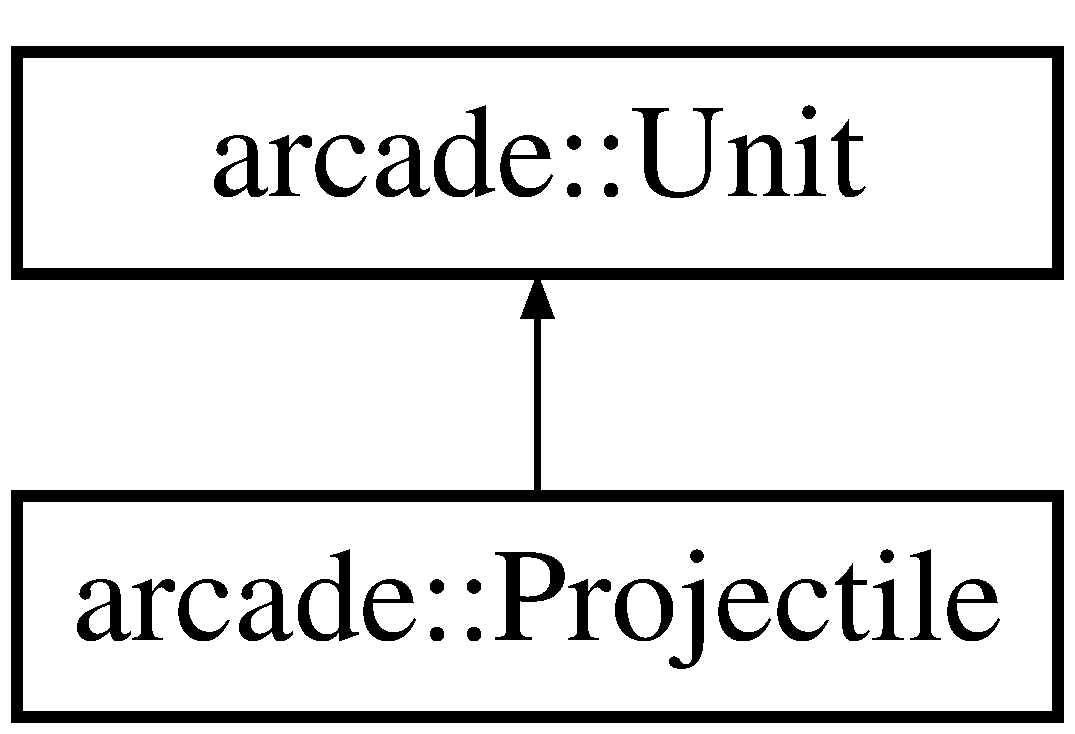
\includegraphics[height=2.000000cm]{classarcade_1_1_projectile}
\end{center}
\end{figure}
\subsection*{Public Member Functions}
\begin{DoxyCompactItemize}
\item 
virtual \hyperlink{classarcade_1_1_projectile_a5307e3fe4f6fe16fc0b4cc03886e56dc}{$\sim$\+Projectile} ()
\item 
\hyperlink{classarcade_1_1_projectile_a9c807e2b75ce47ee02519ae69a7e10b5}{Projectile} (size\+\_\+t \hyperlink{include_2_protocol_8hpp_a4dde988b1b2adba65ae3efa69f65d960}{x}, size\+\_\+t \hyperlink{include_2_protocol_8hpp_ab0580f504a7428539be299fa71565f30}{y}, \hyperlink{classarcade_1_1_unit_af418afeaba1f7fd5934b6ae1343215dd}{Direction} direction, int max\+Range)
\item 
bool \hyperlink{classarcade_1_1_projectile_a109675966eb518e420351a2a6a4dce18}{does\+Collide} (\hyperlink{classarcade_1_1_unit}{Unit} const \&unit) const
\item 
bool \hyperlink{classarcade_1_1_projectile_a991b6754b6a12089b2b527d35f2d3ca9}{move} (\hyperlink{classarcade_1_1_map}{Map} const \&map, \hyperlink{classarcade_1_1_unit}{Unit} const \&unit)
\item 
\hyperlink{classarcade_1_1_unit_af418afeaba1f7fd5934b6ae1343215dd}{Direction} \hyperlink{classarcade_1_1_projectile_a29c62daa5cbdaa3e3dfdcf8265a86913}{get\+Direction} () const
\end{DoxyCompactItemize}
\subsection*{Additional Inherited Members}


\subsection{Constructor \& Destructor Documentation}
\mbox{\Hypertarget{classarcade_1_1_projectile_a5307e3fe4f6fe16fc0b4cc03886e56dc}\label{classarcade_1_1_projectile_a5307e3fe4f6fe16fc0b4cc03886e56dc}} 
\index{arcade\+::\+Projectile@{arcade\+::\+Projectile}!````~Projectile@{$\sim$\+Projectile}}
\index{````~Projectile@{$\sim$\+Projectile}!arcade\+::\+Projectile@{arcade\+::\+Projectile}}
\subsubsection{\texorpdfstring{$\sim$\+Projectile()}{~Projectile()}}
{\footnotesize\ttfamily arcade\+::\+Projectile\+::$\sim$\+Projectile (\begin{DoxyParamCaption}{ }\end{DoxyParamCaption})\hspace{0.3cm}{\ttfamily [virtual]}}

\mbox{\Hypertarget{classarcade_1_1_projectile_a9c807e2b75ce47ee02519ae69a7e10b5}\label{classarcade_1_1_projectile_a9c807e2b75ce47ee02519ae69a7e10b5}} 
\index{arcade\+::\+Projectile@{arcade\+::\+Projectile}!Projectile@{Projectile}}
\index{Projectile@{Projectile}!arcade\+::\+Projectile@{arcade\+::\+Projectile}}
\subsubsection{\texorpdfstring{Projectile()}{Projectile()}}
{\footnotesize\ttfamily arcade\+::\+Projectile\+::\+Projectile (\begin{DoxyParamCaption}\item[{size\+\_\+t}]{x,  }\item[{size\+\_\+t}]{y,  }\item[{\hyperlink{classarcade_1_1_unit_af418afeaba1f7fd5934b6ae1343215dd}{Direction}}]{direction,  }\item[{int}]{max\+Range }\end{DoxyParamCaption})}



\subsection{Member Function Documentation}
\mbox{\Hypertarget{classarcade_1_1_projectile_a109675966eb518e420351a2a6a4dce18}\label{classarcade_1_1_projectile_a109675966eb518e420351a2a6a4dce18}} 
\index{arcade\+::\+Projectile@{arcade\+::\+Projectile}!does\+Collide@{does\+Collide}}
\index{does\+Collide@{does\+Collide}!arcade\+::\+Projectile@{arcade\+::\+Projectile}}
\subsubsection{\texorpdfstring{does\+Collide()}{doesCollide()}}
{\footnotesize\ttfamily bool arcade\+::\+Projectile\+::does\+Collide (\begin{DoxyParamCaption}\item[{\hyperlink{classarcade_1_1_unit}{Unit} const \&}]{unit }\end{DoxyParamCaption}) const}

\mbox{\Hypertarget{classarcade_1_1_projectile_a29c62daa5cbdaa3e3dfdcf8265a86913}\label{classarcade_1_1_projectile_a29c62daa5cbdaa3e3dfdcf8265a86913}} 
\index{arcade\+::\+Projectile@{arcade\+::\+Projectile}!get\+Direction@{get\+Direction}}
\index{get\+Direction@{get\+Direction}!arcade\+::\+Projectile@{arcade\+::\+Projectile}}
\subsubsection{\texorpdfstring{get\+Direction()}{getDirection()}}
{\footnotesize\ttfamily \hyperlink{classarcade_1_1_unit_af418afeaba1f7fd5934b6ae1343215dd}{arcade\+::\+Unit\+::\+Direction} arcade\+::\+Projectile\+::get\+Direction (\begin{DoxyParamCaption}{ }\end{DoxyParamCaption}) const}

\mbox{\Hypertarget{classarcade_1_1_projectile_a991b6754b6a12089b2b527d35f2d3ca9}\label{classarcade_1_1_projectile_a991b6754b6a12089b2b527d35f2d3ca9}} 
\index{arcade\+::\+Projectile@{arcade\+::\+Projectile}!move@{move}}
\index{move@{move}!arcade\+::\+Projectile@{arcade\+::\+Projectile}}
\subsubsection{\texorpdfstring{move()}{move()}}
{\footnotesize\ttfamily bool arcade\+::\+Projectile\+::move (\begin{DoxyParamCaption}\item[{\hyperlink{classarcade_1_1_map}{Map} const \&}]{map,  }\item[{\hyperlink{classarcade_1_1_unit}{Unit} const \&}]{unit }\end{DoxyParamCaption})}



The documentation for this class was generated from the following files\+:\begin{DoxyCompactItemize}
\item 
games\+Srcs/solar\+Fox/\hyperlink{_projectile_8hpp}{Projectile.\+hpp}\item 
games\+Srcs/solar\+Fox/\hyperlink{_projectile_8cpp}{Projectile.\+cpp}\end{DoxyCompactItemize}

\hypertarget{classarcade_1_1_snake_game}{}\section{arcade\+:\+:Snake\+Game Class Reference}
\label{classarcade_1_1_snake_game}\index{arcade\+::\+Snake\+Game@{arcade\+::\+Snake\+Game}}


{\ttfamily \#include $<$Snake\+Game.\+hpp$>$}

Inheritance diagram for arcade\+:\+:Snake\+Game\+:\begin{figure}[H]
\begin{center}
\leavevmode
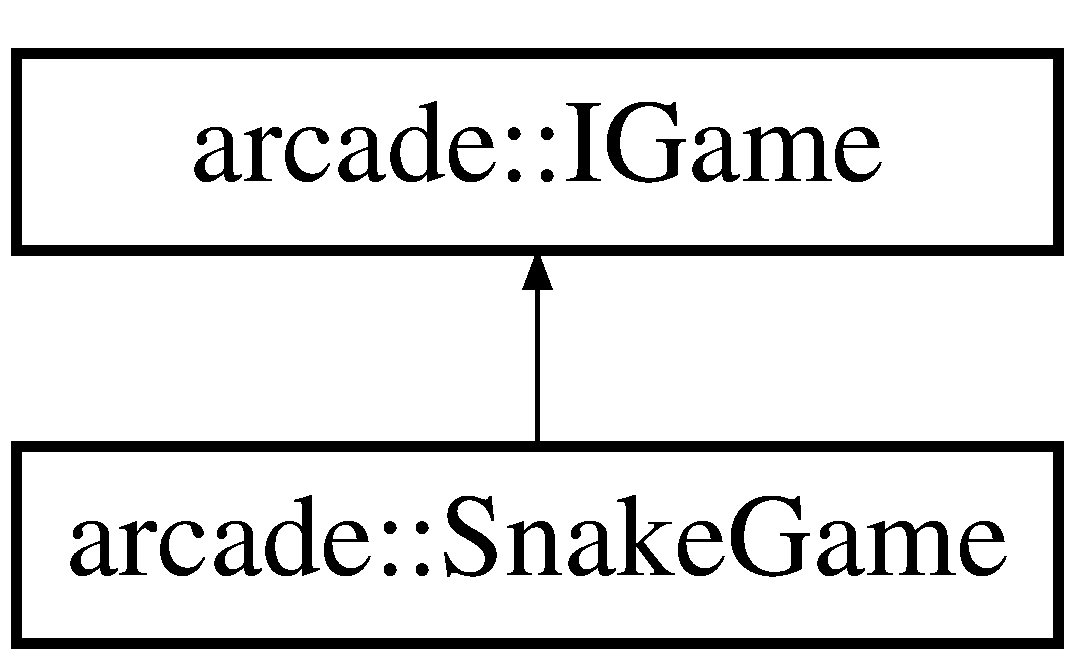
\includegraphics[height=2.000000cm]{classarcade_1_1_snake_game}
\end{center}
\end{figure}
\subsection*{Public Member Functions}
\begin{DoxyCompactItemize}
\item 
virtual \hyperlink{classarcade_1_1_snake_game_a9823e31ef82d6be7689a45933097a554}{$\sim$\+Snake\+Game} ()
\item 
\hyperlink{classarcade_1_1_snake_game_afe35e7494c88ea5a54061d70aecda9e2}{Snake\+Game} ()
\item 
\hyperlink{classarcade_1_1_snake_unit}{Snake\+Unit} \& \hyperlink{classarcade_1_1_snake_game_a4b709bb4139eac56f4f63461ac4324a3}{get\+Snake} ()
\item 
\hyperlink{namespacearcade_a6adca89ee2f539b03980c7e59b044ed7}{Game\+State} \hyperlink{classarcade_1_1_snake_game_afcd7d113f2187cd34396022af4e9e10c}{get\+Game\+State} () const override
\begin{DoxyCompactList}\small\item\em Ask the current game state to the game. \end{DoxyCompactList}\item 
void \hyperlink{classarcade_1_1_snake_game_a93016697def74ebd53a76e33fbb0e583}{notify\+Event} (std\+::vector$<$ \hyperlink{structarcade_1_1_event}{Event} $>$ \&\&events) override
\begin{DoxyCompactList}\small\item\em Send events (keyboard, mouse, etc) to the game. \end{DoxyCompactList}\item 
void \hyperlink{classarcade_1_1_snake_game_a8b4a36ff6ce940d86894433e88bb50f5}{notify\+Network} (std\+::vector$<$ \hyperlink{structarcade_1_1_network_packet}{Network\+Packet} $>$ \&\&events) override
\begin{DoxyCompactList}\small\item\em Send network packets to the game. \end{DoxyCompactList}\item 
std\+::vector$<$ \hyperlink{structarcade_1_1_network_packet}{Network\+Packet} $>$ \hyperlink{classarcade_1_1_snake_game_a8666c3ad148b7140658b52a262bfab73}{get\+Network\+To\+Send} () override
\begin{DoxyCompactList}\small\item\em Get the network packet to send from the game to the server. \end{DoxyCompactList}\item 
bool \hyperlink{classarcade_1_1_snake_game_aa93dbf6b52cb70629abbf646ed33374f}{has\+Network} () const override
\begin{DoxyCompactList}\small\item\em Does this game support network ? \end{DoxyCompactList}\item 
std\+::vector$<$ std\+::unique\+\_\+ptr$<$ \hyperlink{classarcade_1_1_i_sprite}{I\+Sprite} $>$ $>$ \hyperlink{classarcade_1_1_snake_game_aac167f01d2da5121b2f34dd3ca258a45}{get\+Sprites\+To\+Load} () const override
\begin{DoxyCompactList}\small\item\em get the list of sprites to load for this game \end{DoxyCompactList}\item 
std\+::vector$<$ std\+::pair$<$ std\+::string, \hyperlink{namespacearcade_a3bb4743a2eea59f3927e404e6549cae5}{Sound\+Type} $>$ $>$ \hyperlink{classarcade_1_1_snake_game_a2d8ca7114ab012187da99658a221fab9}{get\+Sounds\+To\+Load} () const override
\begin{DoxyCompactList}\small\item\em get the list of sound files to load for this game \end{DoxyCompactList}\item 
\hyperlink{classarcade_1_1_i_g_u_i}{I\+G\+UI} \& \hyperlink{classarcade_1_1_snake_game_ab586312d56bab5be7e1506fa513fea44}{get\+G\+UI} () override
\begin{DoxyCompactList}\small\item\em Get the current version of the \hyperlink{classarcade_1_1_g_u_i}{G\+UI} to display. \end{DoxyCompactList}\item 
std\+::vector$<$ \hyperlink{structarcade_1_1_sound}{Sound} $>$ \hyperlink{classarcade_1_1_snake_game_aab993e72ca1b68914c37209781a68835}{get\+Sounds\+To\+Play} () override
\begin{DoxyCompactList}\small\item\em Get the sounds to play You should return by std\+::move to not copy your vector and to clear it at the same time. \end{DoxyCompactList}\item 
const \hyperlink{classarcade_1_1_i_map}{I\+Map} \& \hyperlink{classarcade_1_1_snake_game_abc3fe4beaa1d2b7df8573f3375cbd4cb}{get\+Current\+Map} () const override
\begin{DoxyCompactList}\small\item\em Get the current version of the map. \end{DoxyCompactList}\item 
const \hyperlink{classarcade_1_1_map}{Map} \& \hyperlink{classarcade_1_1_snake_game_ae11798650684c74dfe0ac61ccb4fc859}{get\+Map} () const
\item 
void \hyperlink{classarcade_1_1_snake_game_a72ed46dfc25cd85c27277705bd93166a}{set\+Acceleration\+Rate} (int acceleration\+Rate)
\item 
void \hyperlink{classarcade_1_1_snake_game_a8a04d76c02f814a01a27f394775ea2f7}{process} () override
\begin{DoxyCompactList}\small\item\em Make the game process a game loop. \end{DoxyCompactList}\item 
void \hyperlink{classarcade_1_1_snake_game_ae35a0091366ec46ab795642ea40d67b9}{spawn\+Apple} ()
\item 
void \hyperlink{classarcade_1_1_snake_game_a5b9b4898677db2d24f993bac6f25c49e}{take\+Apple} (size\+\_\+t \hyperlink{include_2_protocol_8hpp_a4dde988b1b2adba65ae3efa69f65d960}{x}, size\+\_\+t \hyperlink{include_2_protocol_8hpp_ab0580f504a7428539be299fa71565f30}{y})
\item 
void \hyperlink{classarcade_1_1_snake_game_a8d71cb1e19e5158d10e805d152b88fc6}{clear\+Player\+Pos} ()
\item 
void \hyperlink{classarcade_1_1_snake_game_a251558fddc91c0e15d10f413a2633994}{update\+Player\+Pos} ()
\item 
void \hyperlink{classarcade_1_1_snake_game_a508e4f2107e92ff4648254ff421bf1f6}{restart} ()
\end{DoxyCompactItemize}


\subsection{Constructor \& Destructor Documentation}
\mbox{\Hypertarget{classarcade_1_1_snake_game_a9823e31ef82d6be7689a45933097a554}\label{classarcade_1_1_snake_game_a9823e31ef82d6be7689a45933097a554}} 
\index{arcade\+::\+Snake\+Game@{arcade\+::\+Snake\+Game}!````~Snake\+Game@{$\sim$\+Snake\+Game}}
\index{````~Snake\+Game@{$\sim$\+Snake\+Game}!arcade\+::\+Snake\+Game@{arcade\+::\+Snake\+Game}}
\subsubsection{\texorpdfstring{$\sim$\+Snake\+Game()}{~SnakeGame()}}
{\footnotesize\ttfamily arcade\+::\+Snake\+Game\+::$\sim$\+Snake\+Game (\begin{DoxyParamCaption}{ }\end{DoxyParamCaption})\hspace{0.3cm}{\ttfamily [virtual]}}

\mbox{\Hypertarget{classarcade_1_1_snake_game_afe35e7494c88ea5a54061d70aecda9e2}\label{classarcade_1_1_snake_game_afe35e7494c88ea5a54061d70aecda9e2}} 
\index{arcade\+::\+Snake\+Game@{arcade\+::\+Snake\+Game}!Snake\+Game@{Snake\+Game}}
\index{Snake\+Game@{Snake\+Game}!arcade\+::\+Snake\+Game@{arcade\+::\+Snake\+Game}}
\subsubsection{\texorpdfstring{Snake\+Game()}{SnakeGame()}}
{\footnotesize\ttfamily arcade\+::\+Snake\+Game\+::\+Snake\+Game (\begin{DoxyParamCaption}{ }\end{DoxyParamCaption})}



\subsection{Member Function Documentation}
\mbox{\Hypertarget{classarcade_1_1_snake_game_a8d71cb1e19e5158d10e805d152b88fc6}\label{classarcade_1_1_snake_game_a8d71cb1e19e5158d10e805d152b88fc6}} 
\index{arcade\+::\+Snake\+Game@{arcade\+::\+Snake\+Game}!clear\+Player\+Pos@{clear\+Player\+Pos}}
\index{clear\+Player\+Pos@{clear\+Player\+Pos}!arcade\+::\+Snake\+Game@{arcade\+::\+Snake\+Game}}
\subsubsection{\texorpdfstring{clear\+Player\+Pos()}{clearPlayerPos()}}
{\footnotesize\ttfamily void arcade\+::\+Snake\+Game\+::clear\+Player\+Pos (\begin{DoxyParamCaption}{ }\end{DoxyParamCaption})}

\mbox{\Hypertarget{classarcade_1_1_snake_game_abc3fe4beaa1d2b7df8573f3375cbd4cb}\label{classarcade_1_1_snake_game_abc3fe4beaa1d2b7df8573f3375cbd4cb}} 
\index{arcade\+::\+Snake\+Game@{arcade\+::\+Snake\+Game}!get\+Current\+Map@{get\+Current\+Map}}
\index{get\+Current\+Map@{get\+Current\+Map}!arcade\+::\+Snake\+Game@{arcade\+::\+Snake\+Game}}
\subsubsection{\texorpdfstring{get\+Current\+Map()}{getCurrentMap()}}
{\footnotesize\ttfamily const \hyperlink{classarcade_1_1_i_map}{arcade\+::\+I\+Map} \& arcade\+::\+Snake\+Game\+::get\+Current\+Map (\begin{DoxyParamCaption}{ }\end{DoxyParamCaption}) const\hspace{0.3cm}{\ttfamily [override]}, {\ttfamily [virtual]}}



Get the current version of the map. 



Implements \hyperlink{classarcade_1_1_i_game_a2e1791071bf65ee35e249e409ee29044}{arcade\+::\+I\+Game}.

\mbox{\Hypertarget{classarcade_1_1_snake_game_afcd7d113f2187cd34396022af4e9e10c}\label{classarcade_1_1_snake_game_afcd7d113f2187cd34396022af4e9e10c}} 
\index{arcade\+::\+Snake\+Game@{arcade\+::\+Snake\+Game}!get\+Game\+State@{get\+Game\+State}}
\index{get\+Game\+State@{get\+Game\+State}!arcade\+::\+Snake\+Game@{arcade\+::\+Snake\+Game}}
\subsubsection{\texorpdfstring{get\+Game\+State()}{getGameState()}}
{\footnotesize\ttfamily \hyperlink{namespacearcade_a6adca89ee2f539b03980c7e59b044ed7}{arcade\+::\+Game\+State} arcade\+::\+Snake\+Game\+::get\+Game\+State (\begin{DoxyParamCaption}{ }\end{DoxyParamCaption}) const\hspace{0.3cm}{\ttfamily [override]}, {\ttfamily [virtual]}}



Ask the current game state to the game. 



Implements \hyperlink{classarcade_1_1_i_game_a75083f0465c0ccbdbbb38c689b4a694c}{arcade\+::\+I\+Game}.

\mbox{\Hypertarget{classarcade_1_1_snake_game_ab586312d56bab5be7e1506fa513fea44}\label{classarcade_1_1_snake_game_ab586312d56bab5be7e1506fa513fea44}} 
\index{arcade\+::\+Snake\+Game@{arcade\+::\+Snake\+Game}!get\+G\+UI@{get\+G\+UI}}
\index{get\+G\+UI@{get\+G\+UI}!arcade\+::\+Snake\+Game@{arcade\+::\+Snake\+Game}}
\subsubsection{\texorpdfstring{get\+G\+U\+I()}{getGUI()}}
{\footnotesize\ttfamily \hyperlink{classarcade_1_1_i_g_u_i}{arcade\+::\+I\+G\+UI} \& arcade\+::\+Snake\+Game\+::get\+G\+UI (\begin{DoxyParamCaption}{ }\end{DoxyParamCaption})\hspace{0.3cm}{\ttfamily [override]}, {\ttfamily [virtual]}}



Get the current version of the \hyperlink{classarcade_1_1_g_u_i}{G\+UI} to display. 



Implements \hyperlink{classarcade_1_1_i_game_abe849a6ed370a18de51bc8cb7a2329ba}{arcade\+::\+I\+Game}.

\mbox{\Hypertarget{classarcade_1_1_snake_game_ae11798650684c74dfe0ac61ccb4fc859}\label{classarcade_1_1_snake_game_ae11798650684c74dfe0ac61ccb4fc859}} 
\index{arcade\+::\+Snake\+Game@{arcade\+::\+Snake\+Game}!get\+Map@{get\+Map}}
\index{get\+Map@{get\+Map}!arcade\+::\+Snake\+Game@{arcade\+::\+Snake\+Game}}
\subsubsection{\texorpdfstring{get\+Map()}{getMap()}}
{\footnotesize\ttfamily const \hyperlink{classarcade_1_1_map}{arcade\+::\+Map} \& arcade\+::\+Snake\+Game\+::get\+Map (\begin{DoxyParamCaption}{ }\end{DoxyParamCaption}) const}

\mbox{\Hypertarget{classarcade_1_1_snake_game_a8666c3ad148b7140658b52a262bfab73}\label{classarcade_1_1_snake_game_a8666c3ad148b7140658b52a262bfab73}} 
\index{arcade\+::\+Snake\+Game@{arcade\+::\+Snake\+Game}!get\+Network\+To\+Send@{get\+Network\+To\+Send}}
\index{get\+Network\+To\+Send@{get\+Network\+To\+Send}!arcade\+::\+Snake\+Game@{arcade\+::\+Snake\+Game}}
\subsubsection{\texorpdfstring{get\+Network\+To\+Send()}{getNetworkToSend()}}
{\footnotesize\ttfamily std\+::vector$<$ \hyperlink{structarcade_1_1_network_packet}{arcade\+::\+Network\+Packet} $>$ arcade\+::\+Snake\+Game\+::get\+Network\+To\+Send (\begin{DoxyParamCaption}{ }\end{DoxyParamCaption})\hspace{0.3cm}{\ttfamily [override]}, {\ttfamily [virtual]}}



Get the network packet to send from the game to the server. 



Implements \hyperlink{classarcade_1_1_i_game_a5aa80dfdb3c1881fbc749e3d53efc6f8}{arcade\+::\+I\+Game}.

\mbox{\Hypertarget{classarcade_1_1_snake_game_a4b709bb4139eac56f4f63461ac4324a3}\label{classarcade_1_1_snake_game_a4b709bb4139eac56f4f63461ac4324a3}} 
\index{arcade\+::\+Snake\+Game@{arcade\+::\+Snake\+Game}!get\+Snake@{get\+Snake}}
\index{get\+Snake@{get\+Snake}!arcade\+::\+Snake\+Game@{arcade\+::\+Snake\+Game}}
\subsubsection{\texorpdfstring{get\+Snake()}{getSnake()}}
{\footnotesize\ttfamily \hyperlink{classarcade_1_1_snake_unit}{arcade\+::\+Snake\+Unit} \& arcade\+::\+Snake\+Game\+::get\+Snake (\begin{DoxyParamCaption}{ }\end{DoxyParamCaption})}

\mbox{\Hypertarget{classarcade_1_1_snake_game_a2d8ca7114ab012187da99658a221fab9}\label{classarcade_1_1_snake_game_a2d8ca7114ab012187da99658a221fab9}} 
\index{arcade\+::\+Snake\+Game@{arcade\+::\+Snake\+Game}!get\+Sounds\+To\+Load@{get\+Sounds\+To\+Load}}
\index{get\+Sounds\+To\+Load@{get\+Sounds\+To\+Load}!arcade\+::\+Snake\+Game@{arcade\+::\+Snake\+Game}}
\subsubsection{\texorpdfstring{get\+Sounds\+To\+Load()}{getSoundsToLoad()}}
{\footnotesize\ttfamily std\+::vector$<$ std\+::pair$<$ std\+::string, \hyperlink{namespacearcade_a3bb4743a2eea59f3927e404e6549cae5}{arcade\+::\+Sound\+Type} $>$ $>$ arcade\+::\+Snake\+Game\+::get\+Sounds\+To\+Load (\begin{DoxyParamCaption}{ }\end{DoxyParamCaption}) const\hspace{0.3cm}{\ttfamily [override]}, {\ttfamily [virtual]}}



get the list of sound files to load for this game 



Implements \hyperlink{classarcade_1_1_i_game_a0b66cd9ef3b5cd0dff95debb7e4f594e}{arcade\+::\+I\+Game}.

\mbox{\Hypertarget{classarcade_1_1_snake_game_aab993e72ca1b68914c37209781a68835}\label{classarcade_1_1_snake_game_aab993e72ca1b68914c37209781a68835}} 
\index{arcade\+::\+Snake\+Game@{arcade\+::\+Snake\+Game}!get\+Sounds\+To\+Play@{get\+Sounds\+To\+Play}}
\index{get\+Sounds\+To\+Play@{get\+Sounds\+To\+Play}!arcade\+::\+Snake\+Game@{arcade\+::\+Snake\+Game}}
\subsubsection{\texorpdfstring{get\+Sounds\+To\+Play()}{getSoundsToPlay()}}
{\footnotesize\ttfamily std\+::vector$<$ \hyperlink{structarcade_1_1_sound}{arcade\+::\+Sound} $>$ arcade\+::\+Snake\+Game\+::get\+Sounds\+To\+Play (\begin{DoxyParamCaption}{ }\end{DoxyParamCaption})\hspace{0.3cm}{\ttfamily [override]}, {\ttfamily [virtual]}}



Get the sounds to play You should return by std\+::move to not copy your vector and to clear it at the same time. 



Implements \hyperlink{classarcade_1_1_i_game_a88b3c7efb13780cdbbdf5b879a18ed4d}{arcade\+::\+I\+Game}.

\mbox{\Hypertarget{classarcade_1_1_snake_game_aac167f01d2da5121b2f34dd3ca258a45}\label{classarcade_1_1_snake_game_aac167f01d2da5121b2f34dd3ca258a45}} 
\index{arcade\+::\+Snake\+Game@{arcade\+::\+Snake\+Game}!get\+Sprites\+To\+Load@{get\+Sprites\+To\+Load}}
\index{get\+Sprites\+To\+Load@{get\+Sprites\+To\+Load}!arcade\+::\+Snake\+Game@{arcade\+::\+Snake\+Game}}
\subsubsection{\texorpdfstring{get\+Sprites\+To\+Load()}{getSpritesToLoad()}}
{\footnotesize\ttfamily std\+::vector$<$ std\+::unique\+\_\+ptr$<$ \hyperlink{classarcade_1_1_i_sprite}{arcade\+::\+I\+Sprite} $>$ $>$ arcade\+::\+Snake\+Game\+::get\+Sprites\+To\+Load (\begin{DoxyParamCaption}{ }\end{DoxyParamCaption}) const\hspace{0.3cm}{\ttfamily [override]}, {\ttfamily [virtual]}}



get the list of sprites to load for this game 



Implements \hyperlink{classarcade_1_1_i_game_a2d0dc7c78a68c4dd0359911775993f68}{arcade\+::\+I\+Game}.

\mbox{\Hypertarget{classarcade_1_1_snake_game_aa93dbf6b52cb70629abbf646ed33374f}\label{classarcade_1_1_snake_game_aa93dbf6b52cb70629abbf646ed33374f}} 
\index{arcade\+::\+Snake\+Game@{arcade\+::\+Snake\+Game}!has\+Network@{has\+Network}}
\index{has\+Network@{has\+Network}!arcade\+::\+Snake\+Game@{arcade\+::\+Snake\+Game}}
\subsubsection{\texorpdfstring{has\+Network()}{hasNetwork()}}
{\footnotesize\ttfamily bool arcade\+::\+Snake\+Game\+::has\+Network (\begin{DoxyParamCaption}{ }\end{DoxyParamCaption}) const\hspace{0.3cm}{\ttfamily [override]}, {\ttfamily [virtual]}}



Does this game support network ? 



Implements \hyperlink{classarcade_1_1_i_game_ae66bf253e252f43ce17d9e94f08a1d1c}{arcade\+::\+I\+Game}.

\mbox{\Hypertarget{classarcade_1_1_snake_game_a93016697def74ebd53a76e33fbb0e583}\label{classarcade_1_1_snake_game_a93016697def74ebd53a76e33fbb0e583}} 
\index{arcade\+::\+Snake\+Game@{arcade\+::\+Snake\+Game}!notify\+Event@{notify\+Event}}
\index{notify\+Event@{notify\+Event}!arcade\+::\+Snake\+Game@{arcade\+::\+Snake\+Game}}
\subsubsection{\texorpdfstring{notify\+Event()}{notifyEvent()}}
{\footnotesize\ttfamily void arcade\+::\+Snake\+Game\+::notify\+Event (\begin{DoxyParamCaption}\item[{std\+::vector$<$ \hyperlink{structarcade_1_1_event}{Event} $>$ \&\&}]{events }\end{DoxyParamCaption})\hspace{0.3cm}{\ttfamily [override]}, {\ttfamily [virtual]}}



Send events (keyboard, mouse, etc) to the game. 



Implements \hyperlink{classarcade_1_1_i_game_a37d164b4052fa3c28256fb0bf0002876}{arcade\+::\+I\+Game}.

\mbox{\Hypertarget{classarcade_1_1_snake_game_a8b4a36ff6ce940d86894433e88bb50f5}\label{classarcade_1_1_snake_game_a8b4a36ff6ce940d86894433e88bb50f5}} 
\index{arcade\+::\+Snake\+Game@{arcade\+::\+Snake\+Game}!notify\+Network@{notify\+Network}}
\index{notify\+Network@{notify\+Network}!arcade\+::\+Snake\+Game@{arcade\+::\+Snake\+Game}}
\subsubsection{\texorpdfstring{notify\+Network()}{notifyNetwork()}}
{\footnotesize\ttfamily void arcade\+::\+Snake\+Game\+::notify\+Network (\begin{DoxyParamCaption}\item[{std\+::vector$<$ \hyperlink{structarcade_1_1_network_packet}{Network\+Packet} $>$ \&\&}]{events }\end{DoxyParamCaption})\hspace{0.3cm}{\ttfamily [override]}, {\ttfamily [virtual]}}



Send network packets to the game. 



Implements \hyperlink{classarcade_1_1_i_game_aaf375290947abf3db32d966facbfacf3}{arcade\+::\+I\+Game}.

\mbox{\Hypertarget{classarcade_1_1_snake_game_a8a04d76c02f814a01a27f394775ea2f7}\label{classarcade_1_1_snake_game_a8a04d76c02f814a01a27f394775ea2f7}} 
\index{arcade\+::\+Snake\+Game@{arcade\+::\+Snake\+Game}!process@{process}}
\index{process@{process}!arcade\+::\+Snake\+Game@{arcade\+::\+Snake\+Game}}
\subsubsection{\texorpdfstring{process()}{process()}}
{\footnotesize\ttfamily void arcade\+::\+Snake\+Game\+::process (\begin{DoxyParamCaption}{ }\end{DoxyParamCaption})\hspace{0.3cm}{\ttfamily [override]}, {\ttfamily [virtual]}}



Make the game process a game loop. 



Implements \hyperlink{classarcade_1_1_i_game_af0111a41083f38a1af1a7f94287e6e77}{arcade\+::\+I\+Game}.

\mbox{\Hypertarget{classarcade_1_1_snake_game_a508e4f2107e92ff4648254ff421bf1f6}\label{classarcade_1_1_snake_game_a508e4f2107e92ff4648254ff421bf1f6}} 
\index{arcade\+::\+Snake\+Game@{arcade\+::\+Snake\+Game}!restart@{restart}}
\index{restart@{restart}!arcade\+::\+Snake\+Game@{arcade\+::\+Snake\+Game}}
\subsubsection{\texorpdfstring{restart()}{restart()}}
{\footnotesize\ttfamily void arcade\+::\+Snake\+Game\+::restart (\begin{DoxyParamCaption}{ }\end{DoxyParamCaption})}

\mbox{\Hypertarget{classarcade_1_1_snake_game_a72ed46dfc25cd85c27277705bd93166a}\label{classarcade_1_1_snake_game_a72ed46dfc25cd85c27277705bd93166a}} 
\index{arcade\+::\+Snake\+Game@{arcade\+::\+Snake\+Game}!set\+Acceleration\+Rate@{set\+Acceleration\+Rate}}
\index{set\+Acceleration\+Rate@{set\+Acceleration\+Rate}!arcade\+::\+Snake\+Game@{arcade\+::\+Snake\+Game}}
\subsubsection{\texorpdfstring{set\+Acceleration\+Rate()}{setAccelerationRate()}}
{\footnotesize\ttfamily void arcade\+::\+Snake\+Game\+::set\+Acceleration\+Rate (\begin{DoxyParamCaption}\item[{int}]{acceleration\+Rate }\end{DoxyParamCaption})}

\mbox{\Hypertarget{classarcade_1_1_snake_game_ae35a0091366ec46ab795642ea40d67b9}\label{classarcade_1_1_snake_game_ae35a0091366ec46ab795642ea40d67b9}} 
\index{arcade\+::\+Snake\+Game@{arcade\+::\+Snake\+Game}!spawn\+Apple@{spawn\+Apple}}
\index{spawn\+Apple@{spawn\+Apple}!arcade\+::\+Snake\+Game@{arcade\+::\+Snake\+Game}}
\subsubsection{\texorpdfstring{spawn\+Apple()}{spawnApple()}}
{\footnotesize\ttfamily void arcade\+::\+Snake\+Game\+::spawn\+Apple (\begin{DoxyParamCaption}{ }\end{DoxyParamCaption})}

\mbox{\Hypertarget{classarcade_1_1_snake_game_a5b9b4898677db2d24f993bac6f25c49e}\label{classarcade_1_1_snake_game_a5b9b4898677db2d24f993bac6f25c49e}} 
\index{arcade\+::\+Snake\+Game@{arcade\+::\+Snake\+Game}!take\+Apple@{take\+Apple}}
\index{take\+Apple@{take\+Apple}!arcade\+::\+Snake\+Game@{arcade\+::\+Snake\+Game}}
\subsubsection{\texorpdfstring{take\+Apple()}{takeApple()}}
{\footnotesize\ttfamily void arcade\+::\+Snake\+Game\+::take\+Apple (\begin{DoxyParamCaption}\item[{size\+\_\+t}]{x,  }\item[{size\+\_\+t}]{y }\end{DoxyParamCaption})}

\mbox{\Hypertarget{classarcade_1_1_snake_game_a251558fddc91c0e15d10f413a2633994}\label{classarcade_1_1_snake_game_a251558fddc91c0e15d10f413a2633994}} 
\index{arcade\+::\+Snake\+Game@{arcade\+::\+Snake\+Game}!update\+Player\+Pos@{update\+Player\+Pos}}
\index{update\+Player\+Pos@{update\+Player\+Pos}!arcade\+::\+Snake\+Game@{arcade\+::\+Snake\+Game}}
\subsubsection{\texorpdfstring{update\+Player\+Pos()}{updatePlayerPos()}}
{\footnotesize\ttfamily void arcade\+::\+Snake\+Game\+::update\+Player\+Pos (\begin{DoxyParamCaption}{ }\end{DoxyParamCaption})}



The documentation for this class was generated from the following files\+:\begin{DoxyCompactItemize}
\item 
games\+Srcs/snake/\hyperlink{_snake_game_8hpp}{Snake\+Game.\+hpp}\item 
games\+Srcs/snake/\hyperlink{_snake_game_8cpp}{Snake\+Game.\+cpp}\end{DoxyCompactItemize}

\hypertarget{classarcade_1_1_snake_unit}{}\section{arcade\+:\+:Snake\+Unit Class Reference}
\label{classarcade_1_1_snake_unit}\index{arcade\+::\+Snake\+Unit@{arcade\+::\+Snake\+Unit}}


{\ttfamily \#include $<$Snake\+Unit.\+hpp$>$}

Inheritance diagram for arcade\+:\+:Snake\+Unit\+:\begin{figure}[H]
\begin{center}
\leavevmode
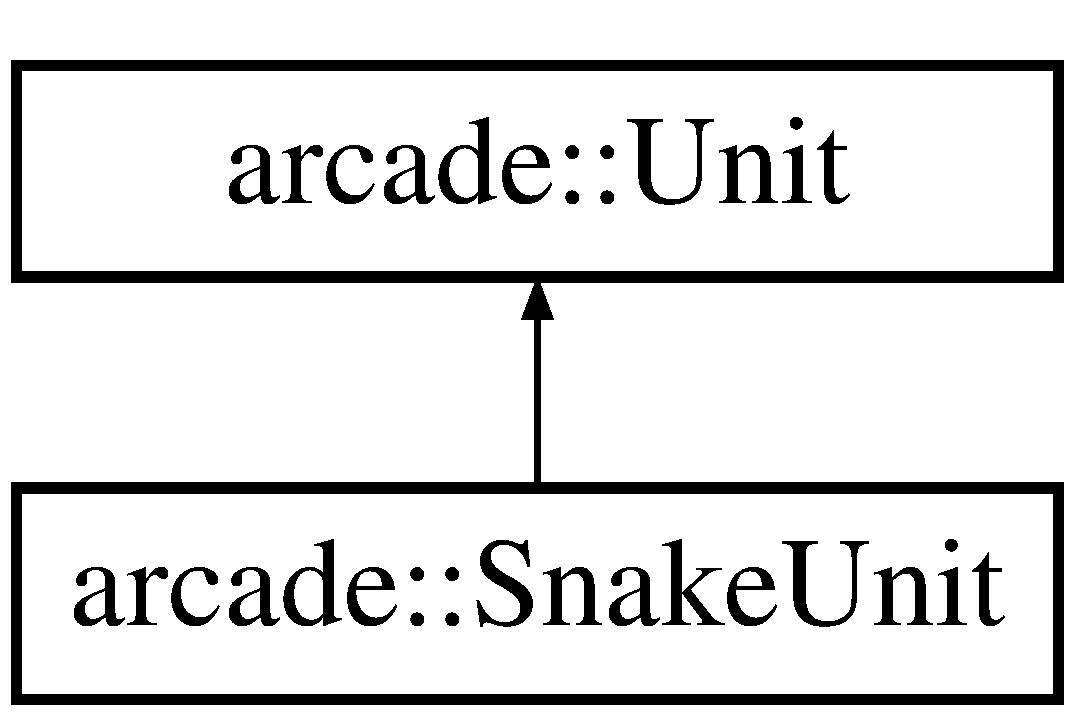
\includegraphics[height=2.000000cm]{classarcade_1_1_snake_unit}
\end{center}
\end{figure}
\subsection*{Public Member Functions}
\begin{DoxyCompactItemize}
\item 
virtual \hyperlink{classarcade_1_1_snake_unit_a797151ca359cb8b6798c24feed6fba45}{$\sim$\+Snake\+Unit} ()
\item 
\hyperlink{classarcade_1_1_snake_unit_a66cb5100f926b000b3931c5fb6dfbfad}{Snake\+Unit} (size\+\_\+t \hyperlink{include_2_protocol_8hpp_a4dde988b1b2adba65ae3efa69f65d960}{x}, size\+\_\+t \hyperlink{include_2_protocol_8hpp_ab0580f504a7428539be299fa71565f30}{y})
\item 
bool \hyperlink{classarcade_1_1_snake_unit_ac291cd07b71f42589e29157fdcf52416}{move} (\hyperlink{classarcade_1_1_map}{Map} const \&map, \hyperlink{classarcade_1_1_unit_af418afeaba1f7fd5934b6ae1343215dd}{Direction} direction) override
\item 
bool \hyperlink{classarcade_1_1_snake_unit_a2a0c1cf1880b9c595706dc0b4202e46a}{move} (\hyperlink{classarcade_1_1_map}{Map} const \&map)
\item 
size\+\_\+t \hyperlink{classarcade_1_1_snake_unit_a7449a250cc1e8c2027e660af40b5454a}{get\+Length} () const
\item 
\hyperlink{classarcade_1_1_unit}{Unit} \& \hyperlink{classarcade_1_1_snake_unit_a29fba4415dc5202deb2b543ea9bcafec}{operator\mbox{[}$\,$\mbox{]}} (size\+\_\+t n)
\item 
\hyperlink{classarcade_1_1_unit}{Unit} \& \hyperlink{classarcade_1_1_snake_unit_a364db276d19b00961a8e445bca7a2d55}{operator\mbox{[}$\,$\mbox{]}} (size\+\_\+t n) const
\item 
\hyperlink{classarcade_1_1_unit_af418afeaba1f7fd5934b6ae1343215dd}{Direction} \hyperlink{classarcade_1_1_snake_unit_a26e52c313c70b4dbc62f0a00f1d29b01}{get\+Moving\+Direction} () const
\item 
void \hyperlink{classarcade_1_1_snake_unit_abc2d43a7920a1bdba452aa888a7e00d1}{set\+Moving\+Direction} (\hyperlink{classarcade_1_1_unit_af418afeaba1f7fd5934b6ae1343215dd}{Direction} moving\+Direction)
\item 
bool \hyperlink{classarcade_1_1_snake_unit_a66b1ed720c9934352f2b23c29ad12b35}{grow} (\hyperlink{classarcade_1_1_map}{Map} const \&map)
\item 
void \hyperlink{classarcade_1_1_snake_unit_aad0f18af64879c5ec44d9f14517abee6}{reset} ()
\end{DoxyCompactItemize}
\subsection*{Additional Inherited Members}


\subsection{Constructor \& Destructor Documentation}
\mbox{\Hypertarget{classarcade_1_1_snake_unit_a797151ca359cb8b6798c24feed6fba45}\label{classarcade_1_1_snake_unit_a797151ca359cb8b6798c24feed6fba45}} 
\index{arcade\+::\+Snake\+Unit@{arcade\+::\+Snake\+Unit}!````~Snake\+Unit@{$\sim$\+Snake\+Unit}}
\index{````~Snake\+Unit@{$\sim$\+Snake\+Unit}!arcade\+::\+Snake\+Unit@{arcade\+::\+Snake\+Unit}}
\subsubsection{\texorpdfstring{$\sim$\+Snake\+Unit()}{~SnakeUnit()}}
{\footnotesize\ttfamily arcade\+::\+Snake\+Unit\+::$\sim$\+Snake\+Unit (\begin{DoxyParamCaption}{ }\end{DoxyParamCaption})\hspace{0.3cm}{\ttfamily [virtual]}}

\mbox{\Hypertarget{classarcade_1_1_snake_unit_a66cb5100f926b000b3931c5fb6dfbfad}\label{classarcade_1_1_snake_unit_a66cb5100f926b000b3931c5fb6dfbfad}} 
\index{arcade\+::\+Snake\+Unit@{arcade\+::\+Snake\+Unit}!Snake\+Unit@{Snake\+Unit}}
\index{Snake\+Unit@{Snake\+Unit}!arcade\+::\+Snake\+Unit@{arcade\+::\+Snake\+Unit}}
\subsubsection{\texorpdfstring{Snake\+Unit()}{SnakeUnit()}}
{\footnotesize\ttfamily arcade\+::\+Snake\+Unit\+::\+Snake\+Unit (\begin{DoxyParamCaption}\item[{size\+\_\+t}]{x,  }\item[{size\+\_\+t}]{y }\end{DoxyParamCaption})}



\subsection{Member Function Documentation}
\mbox{\Hypertarget{classarcade_1_1_snake_unit_a7449a250cc1e8c2027e660af40b5454a}\label{classarcade_1_1_snake_unit_a7449a250cc1e8c2027e660af40b5454a}} 
\index{arcade\+::\+Snake\+Unit@{arcade\+::\+Snake\+Unit}!get\+Length@{get\+Length}}
\index{get\+Length@{get\+Length}!arcade\+::\+Snake\+Unit@{arcade\+::\+Snake\+Unit}}
\subsubsection{\texorpdfstring{get\+Length()}{getLength()}}
{\footnotesize\ttfamily size\+\_\+t arcade\+::\+Snake\+Unit\+::get\+Length (\begin{DoxyParamCaption}{ }\end{DoxyParamCaption}) const}

\mbox{\Hypertarget{classarcade_1_1_snake_unit_a26e52c313c70b4dbc62f0a00f1d29b01}\label{classarcade_1_1_snake_unit_a26e52c313c70b4dbc62f0a00f1d29b01}} 
\index{arcade\+::\+Snake\+Unit@{arcade\+::\+Snake\+Unit}!get\+Moving\+Direction@{get\+Moving\+Direction}}
\index{get\+Moving\+Direction@{get\+Moving\+Direction}!arcade\+::\+Snake\+Unit@{arcade\+::\+Snake\+Unit}}
\subsubsection{\texorpdfstring{get\+Moving\+Direction()}{getMovingDirection()}}
{\footnotesize\ttfamily \hyperlink{classarcade_1_1_unit_af418afeaba1f7fd5934b6ae1343215dd}{arcade\+::\+Unit\+::\+Direction} arcade\+::\+Snake\+Unit\+::get\+Moving\+Direction (\begin{DoxyParamCaption}{ }\end{DoxyParamCaption}) const}

\mbox{\Hypertarget{classarcade_1_1_snake_unit_a66b1ed720c9934352f2b23c29ad12b35}\label{classarcade_1_1_snake_unit_a66b1ed720c9934352f2b23c29ad12b35}} 
\index{arcade\+::\+Snake\+Unit@{arcade\+::\+Snake\+Unit}!grow@{grow}}
\index{grow@{grow}!arcade\+::\+Snake\+Unit@{arcade\+::\+Snake\+Unit}}
\subsubsection{\texorpdfstring{grow()}{grow()}}
{\footnotesize\ttfamily bool arcade\+::\+Snake\+Unit\+::grow (\begin{DoxyParamCaption}\item[{\hyperlink{classarcade_1_1_map}{Map} const \&}]{map }\end{DoxyParamCaption})}

\mbox{\Hypertarget{classarcade_1_1_snake_unit_ac291cd07b71f42589e29157fdcf52416}\label{classarcade_1_1_snake_unit_ac291cd07b71f42589e29157fdcf52416}} 
\index{arcade\+::\+Snake\+Unit@{arcade\+::\+Snake\+Unit}!move@{move}}
\index{move@{move}!arcade\+::\+Snake\+Unit@{arcade\+::\+Snake\+Unit}}
\subsubsection{\texorpdfstring{move()}{move()}\hspace{0.1cm}{\footnotesize\ttfamily [1/2]}}
{\footnotesize\ttfamily bool arcade\+::\+Snake\+Unit\+::move (\begin{DoxyParamCaption}\item[{\hyperlink{classarcade_1_1_map}{Map} const \&}]{map,  }\item[{\hyperlink{classarcade_1_1_unit_af418afeaba1f7fd5934b6ae1343215dd}{Direction}}]{direction }\end{DoxyParamCaption})\hspace{0.3cm}{\ttfamily [override]}, {\ttfamily [virtual]}}



Reimplemented from \hyperlink{classarcade_1_1_unit_a2a6a6feacea0fce220062be1115207b1}{arcade\+::\+Unit}.

\mbox{\Hypertarget{classarcade_1_1_snake_unit_a2a0c1cf1880b9c595706dc0b4202e46a}\label{classarcade_1_1_snake_unit_a2a0c1cf1880b9c595706dc0b4202e46a}} 
\index{arcade\+::\+Snake\+Unit@{arcade\+::\+Snake\+Unit}!move@{move}}
\index{move@{move}!arcade\+::\+Snake\+Unit@{arcade\+::\+Snake\+Unit}}
\subsubsection{\texorpdfstring{move()}{move()}\hspace{0.1cm}{\footnotesize\ttfamily [2/2]}}
{\footnotesize\ttfamily bool arcade\+::\+Snake\+Unit\+::move (\begin{DoxyParamCaption}\item[{\hyperlink{classarcade_1_1_map}{Map} const \&}]{map }\end{DoxyParamCaption})}

\mbox{\Hypertarget{classarcade_1_1_snake_unit_a29fba4415dc5202deb2b543ea9bcafec}\label{classarcade_1_1_snake_unit_a29fba4415dc5202deb2b543ea9bcafec}} 
\index{arcade\+::\+Snake\+Unit@{arcade\+::\+Snake\+Unit}!operator\mbox{[}\mbox{]}@{operator[]}}
\index{operator\mbox{[}\mbox{]}@{operator[]}!arcade\+::\+Snake\+Unit@{arcade\+::\+Snake\+Unit}}
\subsubsection{\texorpdfstring{operator[]()}{operator[]()}\hspace{0.1cm}{\footnotesize\ttfamily [1/2]}}
{\footnotesize\ttfamily \hyperlink{classarcade_1_1_unit}{arcade\+::\+Unit} \& arcade\+::\+Snake\+Unit\+::operator\mbox{[}$\,$\mbox{]} (\begin{DoxyParamCaption}\item[{size\+\_\+t}]{n }\end{DoxyParamCaption})}

\mbox{\Hypertarget{classarcade_1_1_snake_unit_a364db276d19b00961a8e445bca7a2d55}\label{classarcade_1_1_snake_unit_a364db276d19b00961a8e445bca7a2d55}} 
\index{arcade\+::\+Snake\+Unit@{arcade\+::\+Snake\+Unit}!operator\mbox{[}\mbox{]}@{operator[]}}
\index{operator\mbox{[}\mbox{]}@{operator[]}!arcade\+::\+Snake\+Unit@{arcade\+::\+Snake\+Unit}}
\subsubsection{\texorpdfstring{operator[]()}{operator[]()}\hspace{0.1cm}{\footnotesize\ttfamily [2/2]}}
{\footnotesize\ttfamily \hyperlink{classarcade_1_1_unit}{arcade\+::\+Unit} \& arcade\+::\+Snake\+Unit\+::operator\mbox{[}$\,$\mbox{]} (\begin{DoxyParamCaption}\item[{size\+\_\+t}]{n }\end{DoxyParamCaption}) const}

\mbox{\Hypertarget{classarcade_1_1_snake_unit_aad0f18af64879c5ec44d9f14517abee6}\label{classarcade_1_1_snake_unit_aad0f18af64879c5ec44d9f14517abee6}} 
\index{arcade\+::\+Snake\+Unit@{arcade\+::\+Snake\+Unit}!reset@{reset}}
\index{reset@{reset}!arcade\+::\+Snake\+Unit@{arcade\+::\+Snake\+Unit}}
\subsubsection{\texorpdfstring{reset()}{reset()}}
{\footnotesize\ttfamily void arcade\+::\+Snake\+Unit\+::reset (\begin{DoxyParamCaption}{ }\end{DoxyParamCaption})}

\mbox{\Hypertarget{classarcade_1_1_snake_unit_abc2d43a7920a1bdba452aa888a7e00d1}\label{classarcade_1_1_snake_unit_abc2d43a7920a1bdba452aa888a7e00d1}} 
\index{arcade\+::\+Snake\+Unit@{arcade\+::\+Snake\+Unit}!set\+Moving\+Direction@{set\+Moving\+Direction}}
\index{set\+Moving\+Direction@{set\+Moving\+Direction}!arcade\+::\+Snake\+Unit@{arcade\+::\+Snake\+Unit}}
\subsubsection{\texorpdfstring{set\+Moving\+Direction()}{setMovingDirection()}}
{\footnotesize\ttfamily void arcade\+::\+Snake\+Unit\+::set\+Moving\+Direction (\begin{DoxyParamCaption}\item[{\hyperlink{classarcade_1_1_unit_af418afeaba1f7fd5934b6ae1343215dd}{Direction}}]{moving\+Direction }\end{DoxyParamCaption})}



The documentation for this class was generated from the following files\+:\begin{DoxyCompactItemize}
\item 
games\+Srcs/snake/\hyperlink{_snake_unit_8hpp}{Snake\+Unit.\+hpp}\item 
games\+Srcs/snake/\hyperlink{_snake_unit_8cpp}{Snake\+Unit.\+cpp}\end{DoxyCompactItemize}

\hypertarget{classarcade_1_1_solar_fox_game}{}\section{arcade\+:\+:Solar\+Fox\+Game Class Reference}
\label{classarcade_1_1_solar_fox_game}\index{arcade\+::\+Solar\+Fox\+Game@{arcade\+::\+Solar\+Fox\+Game}}


{\ttfamily \#include $<$Solar\+Fox\+Game.\+hpp$>$}

Inheritance diagram for arcade\+:\+:Solar\+Fox\+Game\+:\begin{figure}[H]
\begin{center}
\leavevmode
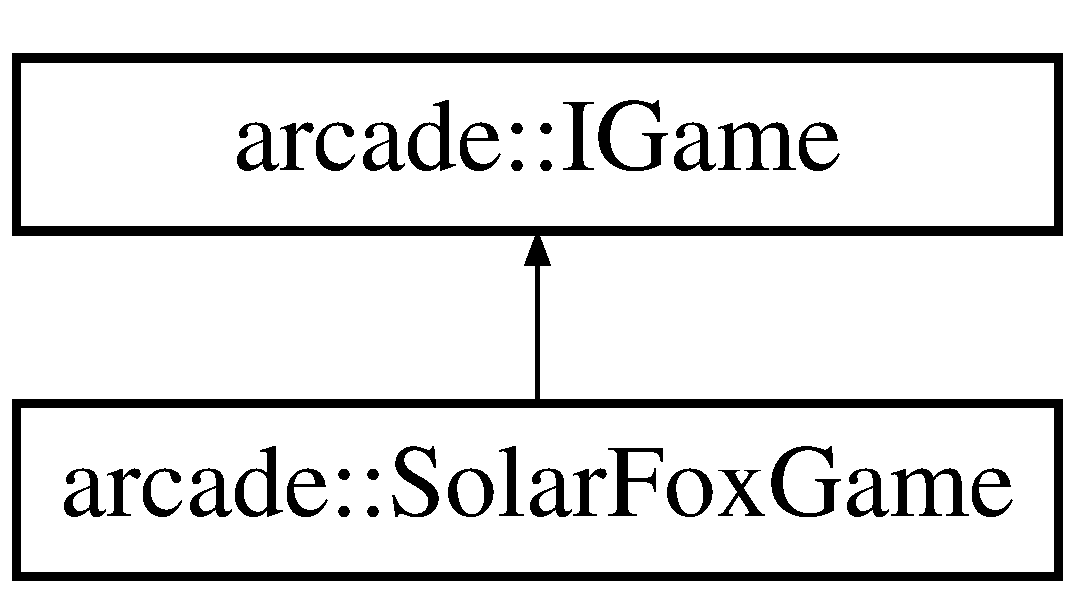
\includegraphics[height=2.000000cm]{classarcade_1_1_solar_fox_game}
\end{center}
\end{figure}
\subsection*{Public Member Functions}
\begin{DoxyCompactItemize}
\item 
virtual \hyperlink{classarcade_1_1_solar_fox_game_ab392eb5aaea9402b947efae9e08147dc}{$\sim$\+Solar\+Fox\+Game} ()
\item 
\hyperlink{classarcade_1_1_solar_fox_game_a8ff7ea5338af65ad2b0f6f038b89b697}{Solar\+Fox\+Game} ()
\item 
\hyperlink{namespacearcade_a6adca89ee2f539b03980c7e59b044ed7}{Game\+State} \hyperlink{classarcade_1_1_solar_fox_game_a71122936c223e672058280755f24a98a}{get\+Game\+State} () const override
\begin{DoxyCompactList}\small\item\em Ask the current game state to the game. \end{DoxyCompactList}\item 
void \hyperlink{classarcade_1_1_solar_fox_game_a12b4c225cad3913bb441a1b208c84bd7}{notify\+Event} (std\+::vector$<$ \hyperlink{structarcade_1_1_event}{Event} $>$ \&\&events) override
\begin{DoxyCompactList}\small\item\em Send events (keyboard, mouse, etc) to the game. \end{DoxyCompactList}\item 
void \hyperlink{classarcade_1_1_solar_fox_game_ada83eb3dae2a14130fca4376f9274e5a}{notify\+Network} (std\+::vector$<$ \hyperlink{structarcade_1_1_network_packet}{Network\+Packet} $>$ \&\&events) override
\begin{DoxyCompactList}\small\item\em Send network packets to the game. \end{DoxyCompactList}\item 
std\+::vector$<$ \hyperlink{structarcade_1_1_network_packet}{Network\+Packet} $>$ \hyperlink{classarcade_1_1_solar_fox_game_a54b56444f83661b4330de868024671d6}{get\+Network\+To\+Send} () override
\begin{DoxyCompactList}\small\item\em Get the network packet to send from the game to the server. \end{DoxyCompactList}\item 
void \hyperlink{classarcade_1_1_solar_fox_game_a12ff0eeb750910455e2dcc1954cdac86}{process} () override
\begin{DoxyCompactList}\small\item\em Make the game process a game loop. \end{DoxyCompactList}\item 
std\+::vector$<$ std\+::unique\+\_\+ptr$<$ \hyperlink{classarcade_1_1_i_sprite}{I\+Sprite} $>$ $>$ \hyperlink{classarcade_1_1_solar_fox_game_afa9d714001212c869f616bd265dd9371}{get\+Sprites\+To\+Load} () const override
\begin{DoxyCompactList}\small\item\em get the list of sprites to load for this game \end{DoxyCompactList}\item 
std\+::vector$<$ std\+::pair$<$ std\+::string, \hyperlink{namespacearcade_a3bb4743a2eea59f3927e404e6549cae5}{Sound\+Type} $>$ $>$ \hyperlink{classarcade_1_1_solar_fox_game_aed75a8fdc63d9162359ada5332b44331}{get\+Sounds\+To\+Load} () const override
\begin{DoxyCompactList}\small\item\em get the list of sound files to load for this game \end{DoxyCompactList}\item 
std\+::vector$<$ \hyperlink{structarcade_1_1_sound}{Sound} $>$ \hyperlink{classarcade_1_1_solar_fox_game_a96f41df94a733d0c06f8a7d48e620d58}{get\+Sounds\+To\+Play} () override
\begin{DoxyCompactList}\small\item\em Get the sounds to play You should return by std\+::move to not copy your vector and to clear it at the same time. \end{DoxyCompactList}\item 
const \hyperlink{classarcade_1_1_i_map}{I\+Map} \& \hyperlink{classarcade_1_1_solar_fox_game_a8bb422466d4367320e90c6f9c6b754ed}{get\+Current\+Map} () const override
\begin{DoxyCompactList}\small\item\em Get the current version of the map. \end{DoxyCompactList}\item 
const \hyperlink{classarcade_1_1_map}{Map} \& \hyperlink{classarcade_1_1_solar_fox_game_a89c8912a012a8283f8509e243c4d5b0b}{get\+Map} () const
\item 
\hyperlink{classarcade_1_1_i_g_u_i}{I\+G\+UI} \& \hyperlink{classarcade_1_1_solar_fox_game_aba8a5d93b17231c5d2cbbb51cc1d05b9}{get\+G\+UI} () override
\begin{DoxyCompactList}\small\item\em Get the current version of the \hyperlink{classarcade_1_1_g_u_i}{G\+UI} to display. \end{DoxyCompactList}\item 
void \hyperlink{classarcade_1_1_solar_fox_game_a6e846bc8d6fbd3752c5342bfb682e9cb}{set\+Acceleration\+Rate} (int acceleration\+Rate)
\item 
\hyperlink{classarcade_1_1_spaceship}{Spaceship} \& \hyperlink{classarcade_1_1_solar_fox_game_a75c60a8ae25175073200318d3d2072fd}{get\+Player} ()
\item 
void \hyperlink{classarcade_1_1_solar_fox_game_a60c1aad9687dea93c752717672ae31fc}{restart} ()
\item 
bool \hyperlink{classarcade_1_1_solar_fox_game_a4142a002e8b141216c67638ba7a118d3}{has\+Network} () const override
\begin{DoxyCompactList}\small\item\em Does this game support network ? \end{DoxyCompactList}\end{DoxyCompactItemize}


\subsection{Constructor \& Destructor Documentation}
\mbox{\Hypertarget{classarcade_1_1_solar_fox_game_ab392eb5aaea9402b947efae9e08147dc}\label{classarcade_1_1_solar_fox_game_ab392eb5aaea9402b947efae9e08147dc}} 
\index{arcade\+::\+Solar\+Fox\+Game@{arcade\+::\+Solar\+Fox\+Game}!````~Solar\+Fox\+Game@{$\sim$\+Solar\+Fox\+Game}}
\index{````~Solar\+Fox\+Game@{$\sim$\+Solar\+Fox\+Game}!arcade\+::\+Solar\+Fox\+Game@{arcade\+::\+Solar\+Fox\+Game}}
\subsubsection{\texorpdfstring{$\sim$\+Solar\+Fox\+Game()}{~SolarFoxGame()}}
{\footnotesize\ttfamily arcade\+::\+Solar\+Fox\+Game\+::$\sim$\+Solar\+Fox\+Game (\begin{DoxyParamCaption}{ }\end{DoxyParamCaption})\hspace{0.3cm}{\ttfamily [virtual]}}

\mbox{\Hypertarget{classarcade_1_1_solar_fox_game_a8ff7ea5338af65ad2b0f6f038b89b697}\label{classarcade_1_1_solar_fox_game_a8ff7ea5338af65ad2b0f6f038b89b697}} 
\index{arcade\+::\+Solar\+Fox\+Game@{arcade\+::\+Solar\+Fox\+Game}!Solar\+Fox\+Game@{Solar\+Fox\+Game}}
\index{Solar\+Fox\+Game@{Solar\+Fox\+Game}!arcade\+::\+Solar\+Fox\+Game@{arcade\+::\+Solar\+Fox\+Game}}
\subsubsection{\texorpdfstring{Solar\+Fox\+Game()}{SolarFoxGame()}}
{\footnotesize\ttfamily arcade\+::\+Solar\+Fox\+Game\+::\+Solar\+Fox\+Game (\begin{DoxyParamCaption}{ }\end{DoxyParamCaption})}



\subsection{Member Function Documentation}
\mbox{\Hypertarget{classarcade_1_1_solar_fox_game_a8bb422466d4367320e90c6f9c6b754ed}\label{classarcade_1_1_solar_fox_game_a8bb422466d4367320e90c6f9c6b754ed}} 
\index{arcade\+::\+Solar\+Fox\+Game@{arcade\+::\+Solar\+Fox\+Game}!get\+Current\+Map@{get\+Current\+Map}}
\index{get\+Current\+Map@{get\+Current\+Map}!arcade\+::\+Solar\+Fox\+Game@{arcade\+::\+Solar\+Fox\+Game}}
\subsubsection{\texorpdfstring{get\+Current\+Map()}{getCurrentMap()}}
{\footnotesize\ttfamily const \hyperlink{classarcade_1_1_i_map}{arcade\+::\+I\+Map} \& arcade\+::\+Solar\+Fox\+Game\+::get\+Current\+Map (\begin{DoxyParamCaption}{ }\end{DoxyParamCaption}) const\hspace{0.3cm}{\ttfamily [override]}, {\ttfamily [virtual]}}



Get the current version of the map. 



Implements \hyperlink{classarcade_1_1_i_game_a2e1791071bf65ee35e249e409ee29044}{arcade\+::\+I\+Game}.

\mbox{\Hypertarget{classarcade_1_1_solar_fox_game_a71122936c223e672058280755f24a98a}\label{classarcade_1_1_solar_fox_game_a71122936c223e672058280755f24a98a}} 
\index{arcade\+::\+Solar\+Fox\+Game@{arcade\+::\+Solar\+Fox\+Game}!get\+Game\+State@{get\+Game\+State}}
\index{get\+Game\+State@{get\+Game\+State}!arcade\+::\+Solar\+Fox\+Game@{arcade\+::\+Solar\+Fox\+Game}}
\subsubsection{\texorpdfstring{get\+Game\+State()}{getGameState()}}
{\footnotesize\ttfamily \hyperlink{namespacearcade_a6adca89ee2f539b03980c7e59b044ed7}{arcade\+::\+Game\+State} arcade\+::\+Solar\+Fox\+Game\+::get\+Game\+State (\begin{DoxyParamCaption}{ }\end{DoxyParamCaption}) const\hspace{0.3cm}{\ttfamily [override]}, {\ttfamily [virtual]}}



Ask the current game state to the game. 



Implements \hyperlink{classarcade_1_1_i_game_a75083f0465c0ccbdbbb38c689b4a694c}{arcade\+::\+I\+Game}.

\mbox{\Hypertarget{classarcade_1_1_solar_fox_game_aba8a5d93b17231c5d2cbbb51cc1d05b9}\label{classarcade_1_1_solar_fox_game_aba8a5d93b17231c5d2cbbb51cc1d05b9}} 
\index{arcade\+::\+Solar\+Fox\+Game@{arcade\+::\+Solar\+Fox\+Game}!get\+G\+UI@{get\+G\+UI}}
\index{get\+G\+UI@{get\+G\+UI}!arcade\+::\+Solar\+Fox\+Game@{arcade\+::\+Solar\+Fox\+Game}}
\subsubsection{\texorpdfstring{get\+G\+U\+I()}{getGUI()}}
{\footnotesize\ttfamily \hyperlink{classarcade_1_1_i_g_u_i}{arcade\+::\+I\+G\+UI} \& arcade\+::\+Solar\+Fox\+Game\+::get\+G\+UI (\begin{DoxyParamCaption}{ }\end{DoxyParamCaption})\hspace{0.3cm}{\ttfamily [override]}, {\ttfamily [virtual]}}



Get the current version of the \hyperlink{classarcade_1_1_g_u_i}{G\+UI} to display. 



Implements \hyperlink{classarcade_1_1_i_game_abe849a6ed370a18de51bc8cb7a2329ba}{arcade\+::\+I\+Game}.

\mbox{\Hypertarget{classarcade_1_1_solar_fox_game_a89c8912a012a8283f8509e243c4d5b0b}\label{classarcade_1_1_solar_fox_game_a89c8912a012a8283f8509e243c4d5b0b}} 
\index{arcade\+::\+Solar\+Fox\+Game@{arcade\+::\+Solar\+Fox\+Game}!get\+Map@{get\+Map}}
\index{get\+Map@{get\+Map}!arcade\+::\+Solar\+Fox\+Game@{arcade\+::\+Solar\+Fox\+Game}}
\subsubsection{\texorpdfstring{get\+Map()}{getMap()}}
{\footnotesize\ttfamily const \hyperlink{classarcade_1_1_map}{arcade\+::\+Map} \& arcade\+::\+Solar\+Fox\+Game\+::get\+Map (\begin{DoxyParamCaption}{ }\end{DoxyParamCaption}) const}

\mbox{\Hypertarget{classarcade_1_1_solar_fox_game_a54b56444f83661b4330de868024671d6}\label{classarcade_1_1_solar_fox_game_a54b56444f83661b4330de868024671d6}} 
\index{arcade\+::\+Solar\+Fox\+Game@{arcade\+::\+Solar\+Fox\+Game}!get\+Network\+To\+Send@{get\+Network\+To\+Send}}
\index{get\+Network\+To\+Send@{get\+Network\+To\+Send}!arcade\+::\+Solar\+Fox\+Game@{arcade\+::\+Solar\+Fox\+Game}}
\subsubsection{\texorpdfstring{get\+Network\+To\+Send()}{getNetworkToSend()}}
{\footnotesize\ttfamily std\+::vector$<$ \hyperlink{structarcade_1_1_network_packet}{arcade\+::\+Network\+Packet} $>$ arcade\+::\+Solar\+Fox\+Game\+::get\+Network\+To\+Send (\begin{DoxyParamCaption}{ }\end{DoxyParamCaption})\hspace{0.3cm}{\ttfamily [override]}, {\ttfamily [virtual]}}



Get the network packet to send from the game to the server. 



Implements \hyperlink{classarcade_1_1_i_game_a5aa80dfdb3c1881fbc749e3d53efc6f8}{arcade\+::\+I\+Game}.

\mbox{\Hypertarget{classarcade_1_1_solar_fox_game_a75c60a8ae25175073200318d3d2072fd}\label{classarcade_1_1_solar_fox_game_a75c60a8ae25175073200318d3d2072fd}} 
\index{arcade\+::\+Solar\+Fox\+Game@{arcade\+::\+Solar\+Fox\+Game}!get\+Player@{get\+Player}}
\index{get\+Player@{get\+Player}!arcade\+::\+Solar\+Fox\+Game@{arcade\+::\+Solar\+Fox\+Game}}
\subsubsection{\texorpdfstring{get\+Player()}{getPlayer()}}
{\footnotesize\ttfamily \hyperlink{classarcade_1_1_spaceship}{arcade\+::\+Spaceship} \& arcade\+::\+Solar\+Fox\+Game\+::get\+Player (\begin{DoxyParamCaption}{ }\end{DoxyParamCaption})}

\mbox{\Hypertarget{classarcade_1_1_solar_fox_game_aed75a8fdc63d9162359ada5332b44331}\label{classarcade_1_1_solar_fox_game_aed75a8fdc63d9162359ada5332b44331}} 
\index{arcade\+::\+Solar\+Fox\+Game@{arcade\+::\+Solar\+Fox\+Game}!get\+Sounds\+To\+Load@{get\+Sounds\+To\+Load}}
\index{get\+Sounds\+To\+Load@{get\+Sounds\+To\+Load}!arcade\+::\+Solar\+Fox\+Game@{arcade\+::\+Solar\+Fox\+Game}}
\subsubsection{\texorpdfstring{get\+Sounds\+To\+Load()}{getSoundsToLoad()}}
{\footnotesize\ttfamily std\+::vector$<$ std\+::pair$<$ std\+::string, \hyperlink{namespacearcade_a3bb4743a2eea59f3927e404e6549cae5}{arcade\+::\+Sound\+Type} $>$ $>$ arcade\+::\+Solar\+Fox\+Game\+::get\+Sounds\+To\+Load (\begin{DoxyParamCaption}{ }\end{DoxyParamCaption}) const\hspace{0.3cm}{\ttfamily [override]}, {\ttfamily [virtual]}}



get the list of sound files to load for this game 



Implements \hyperlink{classarcade_1_1_i_game_a0b66cd9ef3b5cd0dff95debb7e4f594e}{arcade\+::\+I\+Game}.

\mbox{\Hypertarget{classarcade_1_1_solar_fox_game_a96f41df94a733d0c06f8a7d48e620d58}\label{classarcade_1_1_solar_fox_game_a96f41df94a733d0c06f8a7d48e620d58}} 
\index{arcade\+::\+Solar\+Fox\+Game@{arcade\+::\+Solar\+Fox\+Game}!get\+Sounds\+To\+Play@{get\+Sounds\+To\+Play}}
\index{get\+Sounds\+To\+Play@{get\+Sounds\+To\+Play}!arcade\+::\+Solar\+Fox\+Game@{arcade\+::\+Solar\+Fox\+Game}}
\subsubsection{\texorpdfstring{get\+Sounds\+To\+Play()}{getSoundsToPlay()}}
{\footnotesize\ttfamily std\+::vector$<$ \hyperlink{structarcade_1_1_sound}{arcade\+::\+Sound} $>$ arcade\+::\+Solar\+Fox\+Game\+::get\+Sounds\+To\+Play (\begin{DoxyParamCaption}{ }\end{DoxyParamCaption})\hspace{0.3cm}{\ttfamily [override]}, {\ttfamily [virtual]}}



Get the sounds to play You should return by std\+::move to not copy your vector and to clear it at the same time. 



Implements \hyperlink{classarcade_1_1_i_game_a88b3c7efb13780cdbbdf5b879a18ed4d}{arcade\+::\+I\+Game}.

\mbox{\Hypertarget{classarcade_1_1_solar_fox_game_afa9d714001212c869f616bd265dd9371}\label{classarcade_1_1_solar_fox_game_afa9d714001212c869f616bd265dd9371}} 
\index{arcade\+::\+Solar\+Fox\+Game@{arcade\+::\+Solar\+Fox\+Game}!get\+Sprites\+To\+Load@{get\+Sprites\+To\+Load}}
\index{get\+Sprites\+To\+Load@{get\+Sprites\+To\+Load}!arcade\+::\+Solar\+Fox\+Game@{arcade\+::\+Solar\+Fox\+Game}}
\subsubsection{\texorpdfstring{get\+Sprites\+To\+Load()}{getSpritesToLoad()}}
{\footnotesize\ttfamily std\+::vector$<$ std\+::unique\+\_\+ptr$<$ \hyperlink{classarcade_1_1_i_sprite}{arcade\+::\+I\+Sprite} $>$ $>$ arcade\+::\+Solar\+Fox\+Game\+::get\+Sprites\+To\+Load (\begin{DoxyParamCaption}{ }\end{DoxyParamCaption}) const\hspace{0.3cm}{\ttfamily [override]}, {\ttfamily [virtual]}}



get the list of sprites to load for this game 



Implements \hyperlink{classarcade_1_1_i_game_a2d0dc7c78a68c4dd0359911775993f68}{arcade\+::\+I\+Game}.

\mbox{\Hypertarget{classarcade_1_1_solar_fox_game_a4142a002e8b141216c67638ba7a118d3}\label{classarcade_1_1_solar_fox_game_a4142a002e8b141216c67638ba7a118d3}} 
\index{arcade\+::\+Solar\+Fox\+Game@{arcade\+::\+Solar\+Fox\+Game}!has\+Network@{has\+Network}}
\index{has\+Network@{has\+Network}!arcade\+::\+Solar\+Fox\+Game@{arcade\+::\+Solar\+Fox\+Game}}
\subsubsection{\texorpdfstring{has\+Network()}{hasNetwork()}}
{\footnotesize\ttfamily bool arcade\+::\+Solar\+Fox\+Game\+::has\+Network (\begin{DoxyParamCaption}{ }\end{DoxyParamCaption}) const\hspace{0.3cm}{\ttfamily [override]}, {\ttfamily [virtual]}}



Does this game support network ? 



Implements \hyperlink{classarcade_1_1_i_game_ae66bf253e252f43ce17d9e94f08a1d1c}{arcade\+::\+I\+Game}.

\mbox{\Hypertarget{classarcade_1_1_solar_fox_game_a12b4c225cad3913bb441a1b208c84bd7}\label{classarcade_1_1_solar_fox_game_a12b4c225cad3913bb441a1b208c84bd7}} 
\index{arcade\+::\+Solar\+Fox\+Game@{arcade\+::\+Solar\+Fox\+Game}!notify\+Event@{notify\+Event}}
\index{notify\+Event@{notify\+Event}!arcade\+::\+Solar\+Fox\+Game@{arcade\+::\+Solar\+Fox\+Game}}
\subsubsection{\texorpdfstring{notify\+Event()}{notifyEvent()}}
{\footnotesize\ttfamily void arcade\+::\+Solar\+Fox\+Game\+::notify\+Event (\begin{DoxyParamCaption}\item[{std\+::vector$<$ \hyperlink{structarcade_1_1_event}{Event} $>$ \&\&}]{events }\end{DoxyParamCaption})\hspace{0.3cm}{\ttfamily [override]}, {\ttfamily [virtual]}}



Send events (keyboard, mouse, etc) to the game. 



Implements \hyperlink{classarcade_1_1_i_game_a37d164b4052fa3c28256fb0bf0002876}{arcade\+::\+I\+Game}.

\mbox{\Hypertarget{classarcade_1_1_solar_fox_game_ada83eb3dae2a14130fca4376f9274e5a}\label{classarcade_1_1_solar_fox_game_ada83eb3dae2a14130fca4376f9274e5a}} 
\index{arcade\+::\+Solar\+Fox\+Game@{arcade\+::\+Solar\+Fox\+Game}!notify\+Network@{notify\+Network}}
\index{notify\+Network@{notify\+Network}!arcade\+::\+Solar\+Fox\+Game@{arcade\+::\+Solar\+Fox\+Game}}
\subsubsection{\texorpdfstring{notify\+Network()}{notifyNetwork()}}
{\footnotesize\ttfamily void arcade\+::\+Solar\+Fox\+Game\+::notify\+Network (\begin{DoxyParamCaption}\item[{std\+::vector$<$ \hyperlink{structarcade_1_1_network_packet}{Network\+Packet} $>$ \&\&}]{events }\end{DoxyParamCaption})\hspace{0.3cm}{\ttfamily [override]}, {\ttfamily [virtual]}}



Send network packets to the game. 



Implements \hyperlink{classarcade_1_1_i_game_aaf375290947abf3db32d966facbfacf3}{arcade\+::\+I\+Game}.

\mbox{\Hypertarget{classarcade_1_1_solar_fox_game_a12ff0eeb750910455e2dcc1954cdac86}\label{classarcade_1_1_solar_fox_game_a12ff0eeb750910455e2dcc1954cdac86}} 
\index{arcade\+::\+Solar\+Fox\+Game@{arcade\+::\+Solar\+Fox\+Game}!process@{process}}
\index{process@{process}!arcade\+::\+Solar\+Fox\+Game@{arcade\+::\+Solar\+Fox\+Game}}
\subsubsection{\texorpdfstring{process()}{process()}}
{\footnotesize\ttfamily void arcade\+::\+Solar\+Fox\+Game\+::process (\begin{DoxyParamCaption}{ }\end{DoxyParamCaption})\hspace{0.3cm}{\ttfamily [override]}, {\ttfamily [virtual]}}



Make the game process a game loop. 



Implements \hyperlink{classarcade_1_1_i_game_af0111a41083f38a1af1a7f94287e6e77}{arcade\+::\+I\+Game}.

\mbox{\Hypertarget{classarcade_1_1_solar_fox_game_a60c1aad9687dea93c752717672ae31fc}\label{classarcade_1_1_solar_fox_game_a60c1aad9687dea93c752717672ae31fc}} 
\index{arcade\+::\+Solar\+Fox\+Game@{arcade\+::\+Solar\+Fox\+Game}!restart@{restart}}
\index{restart@{restart}!arcade\+::\+Solar\+Fox\+Game@{arcade\+::\+Solar\+Fox\+Game}}
\subsubsection{\texorpdfstring{restart()}{restart()}}
{\footnotesize\ttfamily void arcade\+::\+Solar\+Fox\+Game\+::restart (\begin{DoxyParamCaption}{ }\end{DoxyParamCaption})}

\mbox{\Hypertarget{classarcade_1_1_solar_fox_game_a6e846bc8d6fbd3752c5342bfb682e9cb}\label{classarcade_1_1_solar_fox_game_a6e846bc8d6fbd3752c5342bfb682e9cb}} 
\index{arcade\+::\+Solar\+Fox\+Game@{arcade\+::\+Solar\+Fox\+Game}!set\+Acceleration\+Rate@{set\+Acceleration\+Rate}}
\index{set\+Acceleration\+Rate@{set\+Acceleration\+Rate}!arcade\+::\+Solar\+Fox\+Game@{arcade\+::\+Solar\+Fox\+Game}}
\subsubsection{\texorpdfstring{set\+Acceleration\+Rate()}{setAccelerationRate()}}
{\footnotesize\ttfamily void arcade\+::\+Solar\+Fox\+Game\+::set\+Acceleration\+Rate (\begin{DoxyParamCaption}\item[{int}]{acceleration\+Rate }\end{DoxyParamCaption})}



The documentation for this class was generated from the following files\+:\begin{DoxyCompactItemize}
\item 
games\+Srcs/solar\+Fox/\hyperlink{_solar_fox_game_8hpp}{Solar\+Fox\+Game.\+hpp}\item 
games\+Srcs/solar\+Fox/\hyperlink{_solar_fox_game_8cpp}{Solar\+Fox\+Game.\+cpp}\end{DoxyCompactItemize}

\hypertarget{structarcade_1_1_sound}{}\section{arcade\+:\+:Sound Struct Reference}
\label{structarcade_1_1_sound}\index{arcade\+::\+Sound@{arcade\+::\+Sound}}


{\ttfamily \#include $<$Sound.\+hpp$>$}

\subsection*{Public Member Functions}
\begin{DoxyCompactItemize}
\item 
\hyperlink{structarcade_1_1_sound_a52388728d9750d6f9aee13b19b4b8427}{Sound} (unsigned int \hyperlink{structarcade_1_1_sound_a9bee48a44860d44ddb963621ceb9172b}{id}, \hyperlink{namespacearcade_a31ef30225775697d1aeaf59819ac5051}{Sound\+Action} \hyperlink{structarcade_1_1_sound_a67fc0884cb4d9445ad6c9d9a241a15ef}{mode}=\hyperlink{namespacearcade_a31ef30225775697d1aeaf59819ac5051a0dcacdf4484296a70e9bb6fabe7e3b8a}{U\+N\+I\+Q\+UE}, float \hyperlink{structarcade_1_1_sound_aa80e8832313b76cefcf2e866c4a2e1cc}{volume}=50.\+0f)
\begin{DoxyCompactList}\small\item\em Constructor of a sound. \end{DoxyCompactList}\end{DoxyCompactItemize}
\subsection*{Public Attributes}
\begin{DoxyCompactItemize}
\item 
unsigned int \hyperlink{structarcade_1_1_sound_a9bee48a44860d44ddb963621ceb9172b}{id}
\item 
\hyperlink{namespacearcade_a31ef30225775697d1aeaf59819ac5051}{Sound\+Action} \hyperlink{structarcade_1_1_sound_a67fc0884cb4d9445ad6c9d9a241a15ef}{mode}
\begin{DoxyCompactList}\small\item\em Id of the sound. \end{DoxyCompactList}\item 
float \hyperlink{structarcade_1_1_sound_aa80e8832313b76cefcf2e866c4a2e1cc}{volume}
\begin{DoxyCompactList}\small\item\em Mode of the sound (control) \end{DoxyCompactList}\end{DoxyCompactItemize}


\subsection{Constructor \& Destructor Documentation}
\mbox{\Hypertarget{structarcade_1_1_sound_a52388728d9750d6f9aee13b19b4b8427}\label{structarcade_1_1_sound_a52388728d9750d6f9aee13b19b4b8427}} 
\index{arcade\+::\+Sound@{arcade\+::\+Sound}!Sound@{Sound}}
\index{Sound@{Sound}!arcade\+::\+Sound@{arcade\+::\+Sound}}
\subsubsection{\texorpdfstring{Sound()}{Sound()}}
{\footnotesize\ttfamily arcade\+::\+Sound\+::\+Sound (\begin{DoxyParamCaption}\item[{unsigned int}]{id,  }\item[{\hyperlink{namespacearcade_a31ef30225775697d1aeaf59819ac5051}{Sound\+Action}}]{mode = {\ttfamily \hyperlink{namespacearcade_a31ef30225775697d1aeaf59819ac5051a0dcacdf4484296a70e9bb6fabe7e3b8a}{U\+N\+I\+Q\+UE}},  }\item[{float}]{volume = {\ttfamily 50.0f} }\end{DoxyParamCaption})}



Constructor of a sound. 


\begin{DoxyParams}{Parameters}
{\em id} & Id du son à controller \\
\hline
{\em mode} & Mode du son \\
\hline
{\em type} & Type de son \\
\hline
{\em volume} & Volume du son \\
\hline
\end{DoxyParams}


\subsection{Member Data Documentation}
\mbox{\Hypertarget{structarcade_1_1_sound_a9bee48a44860d44ddb963621ceb9172b}\label{structarcade_1_1_sound_a9bee48a44860d44ddb963621ceb9172b}} 
\index{arcade\+::\+Sound@{arcade\+::\+Sound}!id@{id}}
\index{id@{id}!arcade\+::\+Sound@{arcade\+::\+Sound}}
\subsubsection{\texorpdfstring{id}{id}}
{\footnotesize\ttfamily unsigned int arcade\+::\+Sound\+::id}

\mbox{\Hypertarget{structarcade_1_1_sound_a67fc0884cb4d9445ad6c9d9a241a15ef}\label{structarcade_1_1_sound_a67fc0884cb4d9445ad6c9d9a241a15ef}} 
\index{arcade\+::\+Sound@{arcade\+::\+Sound}!mode@{mode}}
\index{mode@{mode}!arcade\+::\+Sound@{arcade\+::\+Sound}}
\subsubsection{\texorpdfstring{mode}{mode}}
{\footnotesize\ttfamily \hyperlink{namespacearcade_a31ef30225775697d1aeaf59819ac5051}{Sound\+Action} arcade\+::\+Sound\+::mode}



Id of the sound. 

\mbox{\Hypertarget{structarcade_1_1_sound_aa80e8832313b76cefcf2e866c4a2e1cc}\label{structarcade_1_1_sound_aa80e8832313b76cefcf2e866c4a2e1cc}} 
\index{arcade\+::\+Sound@{arcade\+::\+Sound}!volume@{volume}}
\index{volume@{volume}!arcade\+::\+Sound@{arcade\+::\+Sound}}
\subsubsection{\texorpdfstring{volume}{volume}}
{\footnotesize\ttfamily float arcade\+::\+Sound\+::volume}



Mode of the sound (control) 



The documentation for this struct was generated from the following files\+:\begin{DoxyCompactItemize}
\item 
arcade\+Interfaces/\hyperlink{_sound_8hpp}{Sound.\+hpp}\item 
arcade\+Interfaces/\hyperlink{_sound_8cpp}{Sound.\+cpp}\end{DoxyCompactItemize}

\hypertarget{struct_sound_mode}{}\section{Sound\+Mode Struct Reference}
\label{struct_sound_mode}\index{Sound\+Mode@{Sound\+Mode}}


Contain informations on the sound to play and the way of playing it.  




{\ttfamily \#include $<$Sound.\+hpp$>$}



\subsection{Detailed Description}
Contain informations on the sound to play and the way of playing it. 

The documentation for this struct was generated from the following file\+:\begin{DoxyCompactItemize}
\item 
arcade\+Interfaces/\hyperlink{_sound_8hpp}{Sound.\+hpp}\end{DoxyCompactItemize}

\hypertarget{classarcade_1_1_spaceship}{}\section{arcade\+:\+:Spaceship Class Reference}
\label{classarcade_1_1_spaceship}\index{arcade\+::\+Spaceship@{arcade\+::\+Spaceship}}


{\ttfamily \#include $<$Spaceship.\+hpp$>$}

Inheritance diagram for arcade\+:\+:Spaceship\+:\begin{figure}[H]
\begin{center}
\leavevmode
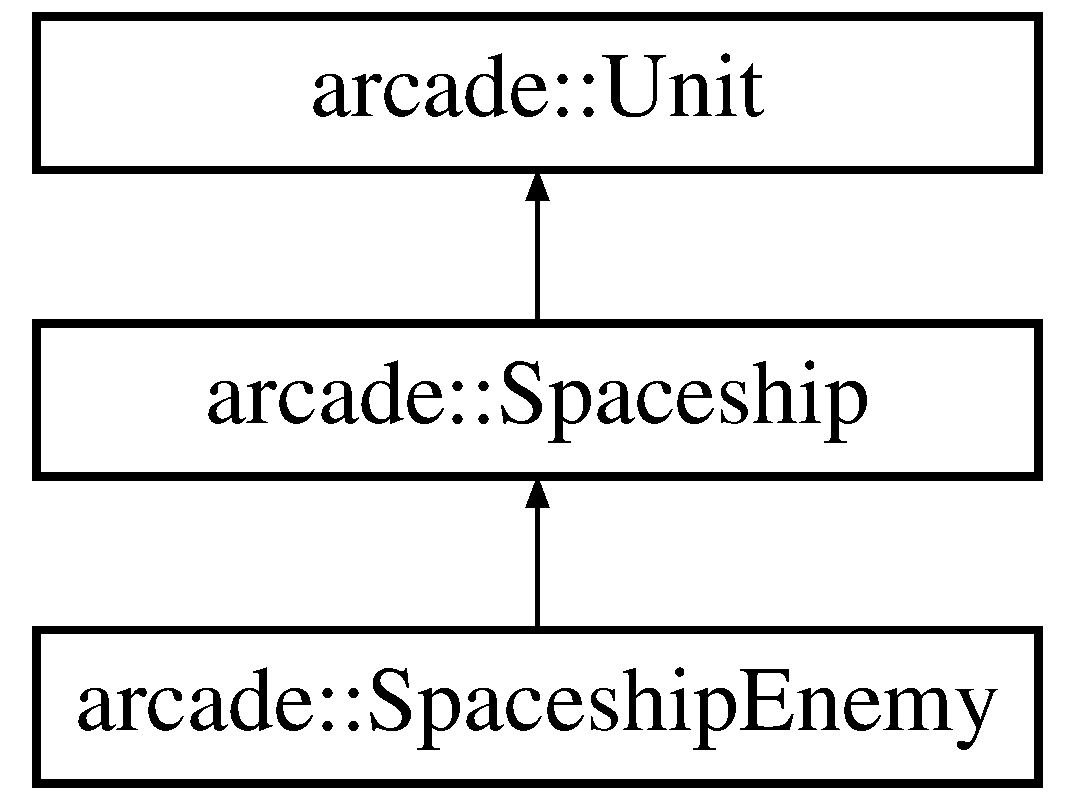
\includegraphics[height=3.000000cm]{classarcade_1_1_spaceship}
\end{center}
\end{figure}
\subsection*{Public Member Functions}
\begin{DoxyCompactItemize}
\item 
virtual \hyperlink{classarcade_1_1_spaceship_ada9cb897bb55ceff50c40228c8307f66}{$\sim$\+Spaceship} ()
\item 
\hyperlink{classarcade_1_1_spaceship_ab9d51b5b611dc512b4e098a6356c8903}{Spaceship} (size\+\_\+t \hyperlink{include_2_protocol_8hpp_a4dde988b1b2adba65ae3efa69f65d960}{x}, size\+\_\+t \hyperlink{include_2_protocol_8hpp_ab0580f504a7428539be299fa71565f30}{y}, int \hyperlink{classarcade_1_1_spaceship_a414281f267135317527aeb86e170d892}{shooting\+Range})
\item 
void \hyperlink{classarcade_1_1_spaceship_aac1226902cf4345e7dc5b91dd6fdf1a4}{set\+Moving\+Direction} (\hyperlink{classarcade_1_1_unit_af418afeaba1f7fd5934b6ae1343215dd}{Direction} \hyperlink{classarcade_1_1_spaceship_a0ac1911c03d0f728e70fca2a9ae01ab2}{moving\+Direction})
\item 
\hyperlink{classarcade_1_1_unit_af418afeaba1f7fd5934b6ae1343215dd}{Direction} \hyperlink{classarcade_1_1_spaceship_a3c768c9647ac59db68f278c1c9cb9f03}{get\+Moving\+Direction} () const
\item 
std\+::vector$<$ \hyperlink{classarcade_1_1_projectile}{Projectile} $\ast$ $>$ \& \hyperlink{classarcade_1_1_spaceship_a3f45b690df3d418a89b042ec12627feb}{get\+Projectiles} ()
\item 
virtual bool \hyperlink{classarcade_1_1_spaceship_a2f13ff685814d14efad398b3564c7646}{does\+Projectiles\+Collide} (\hyperlink{classarcade_1_1_map}{Map} \&map, \hyperlink{classarcade_1_1_unit}{Unit} \&unit)
\item 
virtual bool \hyperlink{classarcade_1_1_spaceship_a2142187204afe7429d4383471769a414}{move} (const \hyperlink{classarcade_1_1_map}{Map} \&map, size\+\_\+t offset\+Map\+Border)
\item 
virtual void \hyperlink{classarcade_1_1_spaceship_a3cac44ed8029c675de7df8dbbff545b4}{shoot} ()
\item 
virtual void \hyperlink{classarcade_1_1_spaceship_aa6a5b59bdb64be086b212847e752b02c}{clear\+Map\+For\+Projectile} (\hyperlink{classarcade_1_1_map}{Map} \&map)
\item 
virtual void \hyperlink{classarcade_1_1_spaceship_acc24a4ca8532c59d2cfb768cae629d8e}{update\+Map\+For\+Projectile} (\hyperlink{classarcade_1_1_map}{Map} \&map, \hyperlink{unionarcade_1_1_color}{Color} color)
\item 
bool \hyperlink{classarcade_1_1_spaceship_af23a861c85c36e432e195ab3cd239058}{does\+Projectiles\+Collide} (\hyperlink{classarcade_1_1_map}{Map} \&map, std\+::vector$<$ \hyperlink{classarcade_1_1_projectile}{arcade\+::\+Projectile} $\ast$$>$ \&units)
\item 
int \hyperlink{classarcade_1_1_spaceship_a7c78ae50bdcb260920a96fb3eb703449}{shoot\+Direction\+To\+Sprite\+Id} (bool player, \hyperlink{classarcade_1_1_unit_af418afeaba1f7fd5934b6ae1343215dd}{arcade\+::\+Unit\+::\+Direction} direction)
\item 
void \hyperlink{classarcade_1_1_spaceship_ab99c1fba278325a45c67224583d800be}{reset} ()
\end{DoxyCompactItemize}
\subsection*{Protected Attributes}
\begin{DoxyCompactItemize}
\item 
std\+::vector$<$ \hyperlink{classarcade_1_1_projectile}{Projectile} $\ast$ $>$ \hyperlink{classarcade_1_1_spaceship_aa91863f21c7e3c05edb90fe3ec3a5ff2}{projectiles}
\item 
\hyperlink{classarcade_1_1_unit_af418afeaba1f7fd5934b6ae1343215dd}{Direction} \hyperlink{classarcade_1_1_spaceship_a0ac1911c03d0f728e70fca2a9ae01ab2}{moving\+Direction}
\item 
int \hyperlink{classarcade_1_1_spaceship_a414281f267135317527aeb86e170d892}{shooting\+Range}
\end{DoxyCompactItemize}
\subsection*{Additional Inherited Members}


\subsection{Constructor \& Destructor Documentation}
\mbox{\Hypertarget{classarcade_1_1_spaceship_ada9cb897bb55ceff50c40228c8307f66}\label{classarcade_1_1_spaceship_ada9cb897bb55ceff50c40228c8307f66}} 
\index{arcade\+::\+Spaceship@{arcade\+::\+Spaceship}!````~Spaceship@{$\sim$\+Spaceship}}
\index{````~Spaceship@{$\sim$\+Spaceship}!arcade\+::\+Spaceship@{arcade\+::\+Spaceship}}
\subsubsection{\texorpdfstring{$\sim$\+Spaceship()}{~Spaceship()}}
{\footnotesize\ttfamily arcade\+::\+Spaceship\+::$\sim$\+Spaceship (\begin{DoxyParamCaption}{ }\end{DoxyParamCaption})\hspace{0.3cm}{\ttfamily [virtual]}}

\mbox{\Hypertarget{classarcade_1_1_spaceship_ab9d51b5b611dc512b4e098a6356c8903}\label{classarcade_1_1_spaceship_ab9d51b5b611dc512b4e098a6356c8903}} 
\index{arcade\+::\+Spaceship@{arcade\+::\+Spaceship}!Spaceship@{Spaceship}}
\index{Spaceship@{Spaceship}!arcade\+::\+Spaceship@{arcade\+::\+Spaceship}}
\subsubsection{\texorpdfstring{Spaceship()}{Spaceship()}}
{\footnotesize\ttfamily arcade\+::\+Spaceship\+::\+Spaceship (\begin{DoxyParamCaption}\item[{size\+\_\+t}]{x,  }\item[{size\+\_\+t}]{y,  }\item[{int}]{shooting\+Range }\end{DoxyParamCaption})}



\subsection{Member Function Documentation}
\mbox{\Hypertarget{classarcade_1_1_spaceship_aa6a5b59bdb64be086b212847e752b02c}\label{classarcade_1_1_spaceship_aa6a5b59bdb64be086b212847e752b02c}} 
\index{arcade\+::\+Spaceship@{arcade\+::\+Spaceship}!clear\+Map\+For\+Projectile@{clear\+Map\+For\+Projectile}}
\index{clear\+Map\+For\+Projectile@{clear\+Map\+For\+Projectile}!arcade\+::\+Spaceship@{arcade\+::\+Spaceship}}
\subsubsection{\texorpdfstring{clear\+Map\+For\+Projectile()}{clearMapForProjectile()}}
{\footnotesize\ttfamily void arcade\+::\+Spaceship\+::clear\+Map\+For\+Projectile (\begin{DoxyParamCaption}\item[{\hyperlink{classarcade_1_1_map}{arcade\+::\+Map} \&}]{map }\end{DoxyParamCaption})\hspace{0.3cm}{\ttfamily [virtual]}}



Reimplemented in \hyperlink{classarcade_1_1_spaceship_enemy_a76ad6511c8dba9850fb70a1633f8cc87}{arcade\+::\+Spaceship\+Enemy}.

\mbox{\Hypertarget{classarcade_1_1_spaceship_a2f13ff685814d14efad398b3564c7646}\label{classarcade_1_1_spaceship_a2f13ff685814d14efad398b3564c7646}} 
\index{arcade\+::\+Spaceship@{arcade\+::\+Spaceship}!does\+Projectiles\+Collide@{does\+Projectiles\+Collide}}
\index{does\+Projectiles\+Collide@{does\+Projectiles\+Collide}!arcade\+::\+Spaceship@{arcade\+::\+Spaceship}}
\subsubsection{\texorpdfstring{does\+Projectiles\+Collide()}{doesProjectilesCollide()}\hspace{0.1cm}{\footnotesize\ttfamily [1/2]}}
{\footnotesize\ttfamily bool arcade\+::\+Spaceship\+::does\+Projectiles\+Collide (\begin{DoxyParamCaption}\item[{\hyperlink{classarcade_1_1_map}{Map} \&}]{map,  }\item[{\hyperlink{classarcade_1_1_unit}{arcade\+::\+Unit} \&}]{unit }\end{DoxyParamCaption})\hspace{0.3cm}{\ttfamily [virtual]}}

\mbox{\Hypertarget{classarcade_1_1_spaceship_af23a861c85c36e432e195ab3cd239058}\label{classarcade_1_1_spaceship_af23a861c85c36e432e195ab3cd239058}} 
\index{arcade\+::\+Spaceship@{arcade\+::\+Spaceship}!does\+Projectiles\+Collide@{does\+Projectiles\+Collide}}
\index{does\+Projectiles\+Collide@{does\+Projectiles\+Collide}!arcade\+::\+Spaceship@{arcade\+::\+Spaceship}}
\subsubsection{\texorpdfstring{does\+Projectiles\+Collide()}{doesProjectilesCollide()}\hspace{0.1cm}{\footnotesize\ttfamily [2/2]}}
{\footnotesize\ttfamily bool arcade\+::\+Spaceship\+::does\+Projectiles\+Collide (\begin{DoxyParamCaption}\item[{\hyperlink{classarcade_1_1_map}{Map} \&}]{map,  }\item[{std\+::vector$<$ \hyperlink{classarcade_1_1_projectile}{arcade\+::\+Projectile} $\ast$$>$ \&}]{units }\end{DoxyParamCaption})}

\mbox{\Hypertarget{classarcade_1_1_spaceship_a3c768c9647ac59db68f278c1c9cb9f03}\label{classarcade_1_1_spaceship_a3c768c9647ac59db68f278c1c9cb9f03}} 
\index{arcade\+::\+Spaceship@{arcade\+::\+Spaceship}!get\+Moving\+Direction@{get\+Moving\+Direction}}
\index{get\+Moving\+Direction@{get\+Moving\+Direction}!arcade\+::\+Spaceship@{arcade\+::\+Spaceship}}
\subsubsection{\texorpdfstring{get\+Moving\+Direction()}{getMovingDirection()}}
{\footnotesize\ttfamily \hyperlink{classarcade_1_1_unit_af418afeaba1f7fd5934b6ae1343215dd}{arcade\+::\+Unit\+::\+Direction} arcade\+::\+Spaceship\+::get\+Moving\+Direction (\begin{DoxyParamCaption}{ }\end{DoxyParamCaption}) const}

\mbox{\Hypertarget{classarcade_1_1_spaceship_a3f45b690df3d418a89b042ec12627feb}\label{classarcade_1_1_spaceship_a3f45b690df3d418a89b042ec12627feb}} 
\index{arcade\+::\+Spaceship@{arcade\+::\+Spaceship}!get\+Projectiles@{get\+Projectiles}}
\index{get\+Projectiles@{get\+Projectiles}!arcade\+::\+Spaceship@{arcade\+::\+Spaceship}}
\subsubsection{\texorpdfstring{get\+Projectiles()}{getProjectiles()}}
{\footnotesize\ttfamily std\+::vector$<$ \hyperlink{classarcade_1_1_projectile}{arcade\+::\+Projectile} $\ast$ $>$ \& arcade\+::\+Spaceship\+::get\+Projectiles (\begin{DoxyParamCaption}{ }\end{DoxyParamCaption})}

\mbox{\Hypertarget{classarcade_1_1_spaceship_a2142187204afe7429d4383471769a414}\label{classarcade_1_1_spaceship_a2142187204afe7429d4383471769a414}} 
\index{arcade\+::\+Spaceship@{arcade\+::\+Spaceship}!move@{move}}
\index{move@{move}!arcade\+::\+Spaceship@{arcade\+::\+Spaceship}}
\subsubsection{\texorpdfstring{move()}{move()}}
{\footnotesize\ttfamily bool arcade\+::\+Spaceship\+::move (\begin{DoxyParamCaption}\item[{const \hyperlink{classarcade_1_1_map}{Map} \&}]{map,  }\item[{size\+\_\+t}]{offset\+Map\+Border }\end{DoxyParamCaption})\hspace{0.3cm}{\ttfamily [virtual]}}

\mbox{\Hypertarget{classarcade_1_1_spaceship_ab99c1fba278325a45c67224583d800be}\label{classarcade_1_1_spaceship_ab99c1fba278325a45c67224583d800be}} 
\index{arcade\+::\+Spaceship@{arcade\+::\+Spaceship}!reset@{reset}}
\index{reset@{reset}!arcade\+::\+Spaceship@{arcade\+::\+Spaceship}}
\subsubsection{\texorpdfstring{reset()}{reset()}}
{\footnotesize\ttfamily void arcade\+::\+Spaceship\+::reset (\begin{DoxyParamCaption}{ }\end{DoxyParamCaption})}

\mbox{\Hypertarget{classarcade_1_1_spaceship_aac1226902cf4345e7dc5b91dd6fdf1a4}\label{classarcade_1_1_spaceship_aac1226902cf4345e7dc5b91dd6fdf1a4}} 
\index{arcade\+::\+Spaceship@{arcade\+::\+Spaceship}!set\+Moving\+Direction@{set\+Moving\+Direction}}
\index{set\+Moving\+Direction@{set\+Moving\+Direction}!arcade\+::\+Spaceship@{arcade\+::\+Spaceship}}
\subsubsection{\texorpdfstring{set\+Moving\+Direction()}{setMovingDirection()}}
{\footnotesize\ttfamily void arcade\+::\+Spaceship\+::set\+Moving\+Direction (\begin{DoxyParamCaption}\item[{\hyperlink{classarcade_1_1_unit_af418afeaba1f7fd5934b6ae1343215dd}{Direction}}]{moving\+Direction }\end{DoxyParamCaption})}

\mbox{\Hypertarget{classarcade_1_1_spaceship_a3cac44ed8029c675de7df8dbbff545b4}\label{classarcade_1_1_spaceship_a3cac44ed8029c675de7df8dbbff545b4}} 
\index{arcade\+::\+Spaceship@{arcade\+::\+Spaceship}!shoot@{shoot}}
\index{shoot@{shoot}!arcade\+::\+Spaceship@{arcade\+::\+Spaceship}}
\subsubsection{\texorpdfstring{shoot()}{shoot()}}
{\footnotesize\ttfamily void arcade\+::\+Spaceship\+::shoot (\begin{DoxyParamCaption}{ }\end{DoxyParamCaption})\hspace{0.3cm}{\ttfamily [virtual]}}

\mbox{\Hypertarget{classarcade_1_1_spaceship_a7c78ae50bdcb260920a96fb3eb703449}\label{classarcade_1_1_spaceship_a7c78ae50bdcb260920a96fb3eb703449}} 
\index{arcade\+::\+Spaceship@{arcade\+::\+Spaceship}!shoot\+Direction\+To\+Sprite\+Id@{shoot\+Direction\+To\+Sprite\+Id}}
\index{shoot\+Direction\+To\+Sprite\+Id@{shoot\+Direction\+To\+Sprite\+Id}!arcade\+::\+Spaceship@{arcade\+::\+Spaceship}}
\subsubsection{\texorpdfstring{shoot\+Direction\+To\+Sprite\+Id()}{shootDirectionToSpriteId()}}
{\footnotesize\ttfamily int arcade\+::\+Spaceship\+::shoot\+Direction\+To\+Sprite\+Id (\begin{DoxyParamCaption}\item[{bool}]{player,  }\item[{\hyperlink{classarcade_1_1_unit_af418afeaba1f7fd5934b6ae1343215dd}{arcade\+::\+Unit\+::\+Direction}}]{direction }\end{DoxyParamCaption})}

\mbox{\Hypertarget{classarcade_1_1_spaceship_acc24a4ca8532c59d2cfb768cae629d8e}\label{classarcade_1_1_spaceship_acc24a4ca8532c59d2cfb768cae629d8e}} 
\index{arcade\+::\+Spaceship@{arcade\+::\+Spaceship}!update\+Map\+For\+Projectile@{update\+Map\+For\+Projectile}}
\index{update\+Map\+For\+Projectile@{update\+Map\+For\+Projectile}!arcade\+::\+Spaceship@{arcade\+::\+Spaceship}}
\subsubsection{\texorpdfstring{update\+Map\+For\+Projectile()}{updateMapForProjectile()}}
{\footnotesize\ttfamily void arcade\+::\+Spaceship\+::update\+Map\+For\+Projectile (\begin{DoxyParamCaption}\item[{\hyperlink{classarcade_1_1_map}{arcade\+::\+Map} \&}]{map,  }\item[{\hyperlink{unionarcade_1_1_color}{Color}}]{color }\end{DoxyParamCaption})\hspace{0.3cm}{\ttfamily [virtual]}}



\subsection{Member Data Documentation}
\mbox{\Hypertarget{classarcade_1_1_spaceship_a0ac1911c03d0f728e70fca2a9ae01ab2}\label{classarcade_1_1_spaceship_a0ac1911c03d0f728e70fca2a9ae01ab2}} 
\index{arcade\+::\+Spaceship@{arcade\+::\+Spaceship}!moving\+Direction@{moving\+Direction}}
\index{moving\+Direction@{moving\+Direction}!arcade\+::\+Spaceship@{arcade\+::\+Spaceship}}
\subsubsection{\texorpdfstring{moving\+Direction}{movingDirection}}
{\footnotesize\ttfamily \hyperlink{classarcade_1_1_unit_af418afeaba1f7fd5934b6ae1343215dd}{Direction} arcade\+::\+Spaceship\+::moving\+Direction\hspace{0.3cm}{\ttfamily [protected]}}

\mbox{\Hypertarget{classarcade_1_1_spaceship_aa91863f21c7e3c05edb90fe3ec3a5ff2}\label{classarcade_1_1_spaceship_aa91863f21c7e3c05edb90fe3ec3a5ff2}} 
\index{arcade\+::\+Spaceship@{arcade\+::\+Spaceship}!projectiles@{projectiles}}
\index{projectiles@{projectiles}!arcade\+::\+Spaceship@{arcade\+::\+Spaceship}}
\subsubsection{\texorpdfstring{projectiles}{projectiles}}
{\footnotesize\ttfamily std\+::vector$<$\hyperlink{classarcade_1_1_projectile}{Projectile} $\ast$$>$ arcade\+::\+Spaceship\+::projectiles\hspace{0.3cm}{\ttfamily [protected]}}

\mbox{\Hypertarget{classarcade_1_1_spaceship_a414281f267135317527aeb86e170d892}\label{classarcade_1_1_spaceship_a414281f267135317527aeb86e170d892}} 
\index{arcade\+::\+Spaceship@{arcade\+::\+Spaceship}!shooting\+Range@{shooting\+Range}}
\index{shooting\+Range@{shooting\+Range}!arcade\+::\+Spaceship@{arcade\+::\+Spaceship}}
\subsubsection{\texorpdfstring{shooting\+Range}{shootingRange}}
{\footnotesize\ttfamily int arcade\+::\+Spaceship\+::shooting\+Range\hspace{0.3cm}{\ttfamily [protected]}}



The documentation for this class was generated from the following files\+:\begin{DoxyCompactItemize}
\item 
games\+Srcs/solar\+Fox/\hyperlink{_spaceship_8hpp}{Spaceship.\+hpp}\item 
games\+Srcs/solar\+Fox/\hyperlink{_spaceship_8cpp}{Spaceship.\+cpp}\end{DoxyCompactItemize}

\hypertarget{classarcade_1_1_spaceship_enemy}{}\section{arcade\+:\+:Spaceship\+Enemy Class Reference}
\label{classarcade_1_1_spaceship_enemy}\index{arcade\+::\+Spaceship\+Enemy@{arcade\+::\+Spaceship\+Enemy}}


{\ttfamily \#include $<$Spaceship\+Enemy.\+hpp$>$}

Inheritance diagram for arcade\+:\+:Spaceship\+Enemy\+:\begin{figure}[H]
\begin{center}
\leavevmode
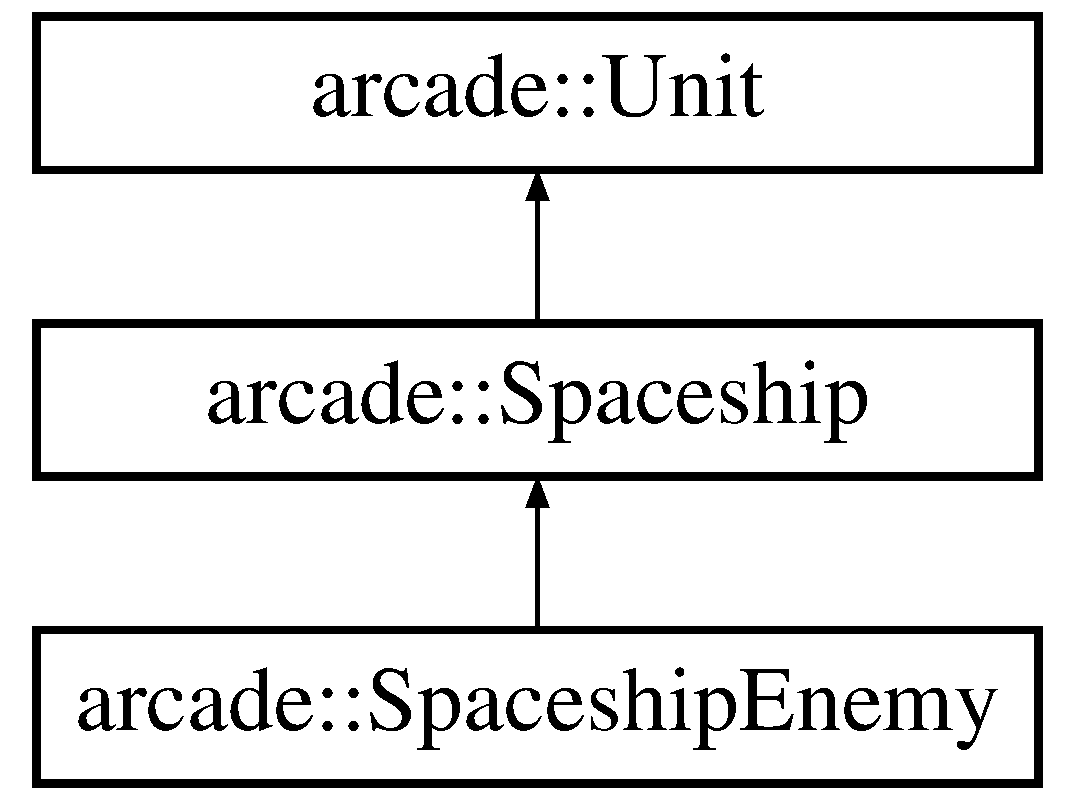
\includegraphics[height=3.000000cm]{classarcade_1_1_spaceship_enemy}
\end{center}
\end{figure}
\subsection*{Public Member Functions}
\begin{DoxyCompactItemize}
\item 
virtual \hyperlink{classarcade_1_1_spaceship_enemy_a7fbb57ede71bf8dde9af2bffc6239bc4}{$\sim$\+Spaceship\+Enemy} ()
\item 
\hyperlink{classarcade_1_1_spaceship_enemy_a1eb27431e53257166ff2c90c8dcf1bc4}{Spaceship\+Enemy} (size\+\_\+t \hyperlink{include_2_protocol_8hpp_a4dde988b1b2adba65ae3efa69f65d960}{x}, size\+\_\+t \hyperlink{include_2_protocol_8hpp_ab0580f504a7428539be299fa71565f30}{y}, int \hyperlink{classarcade_1_1_spaceship_a414281f267135317527aeb86e170d892}{shooting\+Range})
\item 
bool \hyperlink{classarcade_1_1_spaceship_enemy_a62c4ee2725fd8d7496d433bb2ea86603}{move} (const \hyperlink{classarcade_1_1_map}{Map} \&map)
\item 
std\+::pair$<$ int, int $>$ \hyperlink{classarcade_1_1_spaceship_enemy_a6a6b1e32ef2618727bfe01e828a8e4e8}{pos\+Diff\+With\+Player} (\hyperlink{classarcade_1_1_spaceship}{Spaceship} const \&player)
\item 
void \hyperlink{classarcade_1_1_spaceship_enemy_a5b01b4ab0dc3602a1a6f2d93aba67cdd}{choose\+To\+Shoot} (const \hyperlink{classarcade_1_1_map}{Map} \&map, \hyperlink{classarcade_1_1_spaceship}{Spaceship} const \&player)
\item 
bool \hyperlink{classarcade_1_1_spaceship_enemy_a19e3a1d5430307540fba8a649eb06007}{can\+Move} (const \hyperlink{classarcade_1_1_map}{Map} \&map)
\item 
void \hyperlink{classarcade_1_1_spaceship_enemy_ad4963ac1857b42c2497774f77a6d0d05}{shoot} (const \hyperlink{classarcade_1_1_map}{Map} \&map)
\item 
virtual void \hyperlink{classarcade_1_1_spaceship_enemy_a76ad6511c8dba9850fb70a1633f8cc87}{clear\+Map\+For\+Projectile} (\hyperlink{classarcade_1_1_map}{Map} \&map)
\item 
virtual void \hyperlink{classarcade_1_1_spaceship_enemy_acdf6714050c6622c4f67473ec1866404}{update\+Map\+For\+Projectile} (\hyperlink{classarcade_1_1_map}{Map} \&map)
\end{DoxyCompactItemize}
\subsection*{Additional Inherited Members}


\subsection{Constructor \& Destructor Documentation}
\mbox{\Hypertarget{classarcade_1_1_spaceship_enemy_a7fbb57ede71bf8dde9af2bffc6239bc4}\label{classarcade_1_1_spaceship_enemy_a7fbb57ede71bf8dde9af2bffc6239bc4}} 
\index{arcade\+::\+Spaceship\+Enemy@{arcade\+::\+Spaceship\+Enemy}!````~Spaceship\+Enemy@{$\sim$\+Spaceship\+Enemy}}
\index{````~Spaceship\+Enemy@{$\sim$\+Spaceship\+Enemy}!arcade\+::\+Spaceship\+Enemy@{arcade\+::\+Spaceship\+Enemy}}
\subsubsection{\texorpdfstring{$\sim$\+Spaceship\+Enemy()}{~SpaceshipEnemy()}}
{\footnotesize\ttfamily arcade\+::\+Spaceship\+Enemy\+::$\sim$\+Spaceship\+Enemy (\begin{DoxyParamCaption}{ }\end{DoxyParamCaption})\hspace{0.3cm}{\ttfamily [virtual]}}

\mbox{\Hypertarget{classarcade_1_1_spaceship_enemy_a1eb27431e53257166ff2c90c8dcf1bc4}\label{classarcade_1_1_spaceship_enemy_a1eb27431e53257166ff2c90c8dcf1bc4}} 
\index{arcade\+::\+Spaceship\+Enemy@{arcade\+::\+Spaceship\+Enemy}!Spaceship\+Enemy@{Spaceship\+Enemy}}
\index{Spaceship\+Enemy@{Spaceship\+Enemy}!arcade\+::\+Spaceship\+Enemy@{arcade\+::\+Spaceship\+Enemy}}
\subsubsection{\texorpdfstring{Spaceship\+Enemy()}{SpaceshipEnemy()}}
{\footnotesize\ttfamily arcade\+::\+Spaceship\+Enemy\+::\+Spaceship\+Enemy (\begin{DoxyParamCaption}\item[{size\+\_\+t}]{x,  }\item[{size\+\_\+t}]{y,  }\item[{int}]{shooting\+Range }\end{DoxyParamCaption})}



\subsection{Member Function Documentation}
\mbox{\Hypertarget{classarcade_1_1_spaceship_enemy_a19e3a1d5430307540fba8a649eb06007}\label{classarcade_1_1_spaceship_enemy_a19e3a1d5430307540fba8a649eb06007}} 
\index{arcade\+::\+Spaceship\+Enemy@{arcade\+::\+Spaceship\+Enemy}!can\+Move@{can\+Move}}
\index{can\+Move@{can\+Move}!arcade\+::\+Spaceship\+Enemy@{arcade\+::\+Spaceship\+Enemy}}
\subsubsection{\texorpdfstring{can\+Move()}{canMove()}}
{\footnotesize\ttfamily bool arcade\+::\+Spaceship\+Enemy\+::can\+Move (\begin{DoxyParamCaption}\item[{const \hyperlink{classarcade_1_1_map}{Map} \&}]{map }\end{DoxyParamCaption})}

\mbox{\Hypertarget{classarcade_1_1_spaceship_enemy_a5b01b4ab0dc3602a1a6f2d93aba67cdd}\label{classarcade_1_1_spaceship_enemy_a5b01b4ab0dc3602a1a6f2d93aba67cdd}} 
\index{arcade\+::\+Spaceship\+Enemy@{arcade\+::\+Spaceship\+Enemy}!choose\+To\+Shoot@{choose\+To\+Shoot}}
\index{choose\+To\+Shoot@{choose\+To\+Shoot}!arcade\+::\+Spaceship\+Enemy@{arcade\+::\+Spaceship\+Enemy}}
\subsubsection{\texorpdfstring{choose\+To\+Shoot()}{chooseToShoot()}}
{\footnotesize\ttfamily void arcade\+::\+Spaceship\+Enemy\+::choose\+To\+Shoot (\begin{DoxyParamCaption}\item[{const \hyperlink{classarcade_1_1_map}{Map} \&}]{map,  }\item[{\hyperlink{classarcade_1_1_spaceship}{Spaceship} const \&}]{player }\end{DoxyParamCaption})}

\mbox{\Hypertarget{classarcade_1_1_spaceship_enemy_a76ad6511c8dba9850fb70a1633f8cc87}\label{classarcade_1_1_spaceship_enemy_a76ad6511c8dba9850fb70a1633f8cc87}} 
\index{arcade\+::\+Spaceship\+Enemy@{arcade\+::\+Spaceship\+Enemy}!clear\+Map\+For\+Projectile@{clear\+Map\+For\+Projectile}}
\index{clear\+Map\+For\+Projectile@{clear\+Map\+For\+Projectile}!arcade\+::\+Spaceship\+Enemy@{arcade\+::\+Spaceship\+Enemy}}
\subsubsection{\texorpdfstring{clear\+Map\+For\+Projectile()}{clearMapForProjectile()}}
{\footnotesize\ttfamily void arcade\+::\+Spaceship\+Enemy\+::clear\+Map\+For\+Projectile (\begin{DoxyParamCaption}\item[{\hyperlink{classarcade_1_1_map}{arcade\+::\+Map} \&}]{map }\end{DoxyParamCaption})\hspace{0.3cm}{\ttfamily [virtual]}}



Reimplemented from \hyperlink{classarcade_1_1_spaceship_aa6a5b59bdb64be086b212847e752b02c}{arcade\+::\+Spaceship}.

\mbox{\Hypertarget{classarcade_1_1_spaceship_enemy_a62c4ee2725fd8d7496d433bb2ea86603}\label{classarcade_1_1_spaceship_enemy_a62c4ee2725fd8d7496d433bb2ea86603}} 
\index{arcade\+::\+Spaceship\+Enemy@{arcade\+::\+Spaceship\+Enemy}!move@{move}}
\index{move@{move}!arcade\+::\+Spaceship\+Enemy@{arcade\+::\+Spaceship\+Enemy}}
\subsubsection{\texorpdfstring{move()}{move()}}
{\footnotesize\ttfamily bool arcade\+::\+Spaceship\+Enemy\+::move (\begin{DoxyParamCaption}\item[{const \hyperlink{classarcade_1_1_map}{Map} \&}]{map }\end{DoxyParamCaption})}

\mbox{\Hypertarget{classarcade_1_1_spaceship_enemy_a6a6b1e32ef2618727bfe01e828a8e4e8}\label{classarcade_1_1_spaceship_enemy_a6a6b1e32ef2618727bfe01e828a8e4e8}} 
\index{arcade\+::\+Spaceship\+Enemy@{arcade\+::\+Spaceship\+Enemy}!pos\+Diff\+With\+Player@{pos\+Diff\+With\+Player}}
\index{pos\+Diff\+With\+Player@{pos\+Diff\+With\+Player}!arcade\+::\+Spaceship\+Enemy@{arcade\+::\+Spaceship\+Enemy}}
\subsubsection{\texorpdfstring{pos\+Diff\+With\+Player()}{posDiffWithPlayer()}}
{\footnotesize\ttfamily std\+::pair$<$ int, int $>$ arcade\+::\+Spaceship\+Enemy\+::pos\+Diff\+With\+Player (\begin{DoxyParamCaption}\item[{\hyperlink{classarcade_1_1_spaceship}{Spaceship} const \&}]{player }\end{DoxyParamCaption})}

\mbox{\Hypertarget{classarcade_1_1_spaceship_enemy_ad4963ac1857b42c2497774f77a6d0d05}\label{classarcade_1_1_spaceship_enemy_ad4963ac1857b42c2497774f77a6d0d05}} 
\index{arcade\+::\+Spaceship\+Enemy@{arcade\+::\+Spaceship\+Enemy}!shoot@{shoot}}
\index{shoot@{shoot}!arcade\+::\+Spaceship\+Enemy@{arcade\+::\+Spaceship\+Enemy}}
\subsubsection{\texorpdfstring{shoot()}{shoot()}}
{\footnotesize\ttfamily void arcade\+::\+Spaceship\+Enemy\+::shoot (\begin{DoxyParamCaption}\item[{const \hyperlink{classarcade_1_1_map}{Map} \&}]{map }\end{DoxyParamCaption})}

\mbox{\Hypertarget{classarcade_1_1_spaceship_enemy_acdf6714050c6622c4f67473ec1866404}\label{classarcade_1_1_spaceship_enemy_acdf6714050c6622c4f67473ec1866404}} 
\index{arcade\+::\+Spaceship\+Enemy@{arcade\+::\+Spaceship\+Enemy}!update\+Map\+For\+Projectile@{update\+Map\+For\+Projectile}}
\index{update\+Map\+For\+Projectile@{update\+Map\+For\+Projectile}!arcade\+::\+Spaceship\+Enemy@{arcade\+::\+Spaceship\+Enemy}}
\subsubsection{\texorpdfstring{update\+Map\+For\+Projectile()}{updateMapForProjectile()}}
{\footnotesize\ttfamily void arcade\+::\+Spaceship\+Enemy\+::update\+Map\+For\+Projectile (\begin{DoxyParamCaption}\item[{\hyperlink{classarcade_1_1_map}{arcade\+::\+Map} \&}]{map }\end{DoxyParamCaption})\hspace{0.3cm}{\ttfamily [virtual]}}



The documentation for this class was generated from the following files\+:\begin{DoxyCompactItemize}
\item 
games\+Srcs/solar\+Fox/\hyperlink{_spaceship_enemy_8hpp}{Spaceship\+Enemy.\+hpp}\item 
games\+Srcs/solar\+Fox/\hyperlink{_spaceship_enemy_8cpp}{Spaceship\+Enemy.\+cpp}\end{DoxyCompactItemize}

\hypertarget{classarcade_1_1_sprite}{}\section{arcade\+:\+:Sprite Class Reference}
\label{classarcade_1_1_sprite}\index{arcade\+::\+Sprite@{arcade\+::\+Sprite}}


{\ttfamily \#include $<$Sprite.\+hpp$>$}

Inheritance diagram for arcade\+:\+:Sprite\+:\begin{figure}[H]
\begin{center}
\leavevmode
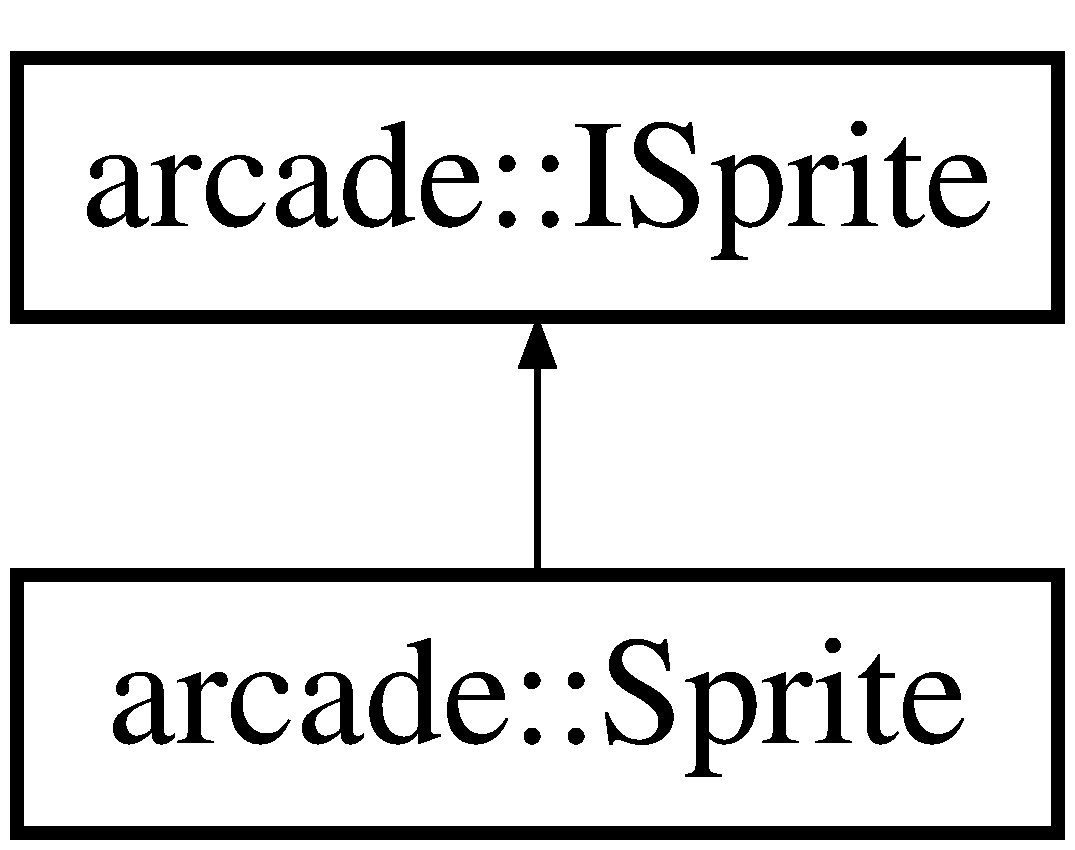
\includegraphics[height=2.000000cm]{classarcade_1_1_sprite}
\end{center}
\end{figure}
\subsection*{Public Member Functions}
\begin{DoxyCompactItemize}
\item 
virtual \hyperlink{classarcade_1_1_sprite_a8e523ec675ab75663ba3fc33743aeb72}{$\sim$\+Sprite} ()
\item 
\hyperlink{classarcade_1_1_sprite_a76833e28f549047d648f2b12694aa6df}{Sprite} (const std\+::vector$<$ std\+::string $>$ \&paths=std\+::vector$<$ std\+::string $>$(), const std\+::vector$<$ char $>$ \&ascii=std\+::vector$<$ char $>$())
\item 
\hyperlink{classarcade_1_1_sprite_ae7194e727354e7b6fd208e0cb72887b4}{Sprite} (\hyperlink{classarcade_1_1_sprite}{Sprite} const \&sprite)
\item 
size\+\_\+t \hyperlink{classarcade_1_1_sprite_a99cc47358f32492ea89659b6b92f4d4c}{sprites\+Count} () const override
\begin{DoxyCompactList}\small\item\em returns the numbers of sprites \end{DoxyCompactList}\item 
std\+::string \hyperlink{classarcade_1_1_sprite_ad8f344724f99ad369c8c552274fface7}{get\+Graphic\+Path} (size\+\_\+t pos) const override
\begin{DoxyCompactList}\small\item\em generates on-\/the-\/fly the path to the sprite at position pos to load \end{DoxyCompactList}\item 
char \hyperlink{classarcade_1_1_sprite_a168a7f537e0fc6d2d4596cab449fde2c}{get\+Ascii} (size\+\_\+t pos) const override
\begin{DoxyCompactList}\small\item\em returns the ascii character at position pos from the animation sequence \end{DoxyCompactList}\end{DoxyCompactItemize}


\subsection{Constructor \& Destructor Documentation}
\mbox{\Hypertarget{classarcade_1_1_sprite_a8e523ec675ab75663ba3fc33743aeb72}\label{classarcade_1_1_sprite_a8e523ec675ab75663ba3fc33743aeb72}} 
\index{arcade\+::\+Sprite@{arcade\+::\+Sprite}!````~Sprite@{$\sim$\+Sprite}}
\index{````~Sprite@{$\sim$\+Sprite}!arcade\+::\+Sprite@{arcade\+::\+Sprite}}
\subsubsection{\texorpdfstring{$\sim$\+Sprite()}{~Sprite()}}
{\footnotesize\ttfamily arcade\+::\+Sprite\+::$\sim$\+Sprite (\begin{DoxyParamCaption}{ }\end{DoxyParamCaption})\hspace{0.3cm}{\ttfamily [virtual]}}

\mbox{\Hypertarget{classarcade_1_1_sprite_a76833e28f549047d648f2b12694aa6df}\label{classarcade_1_1_sprite_a76833e28f549047d648f2b12694aa6df}} 
\index{arcade\+::\+Sprite@{arcade\+::\+Sprite}!Sprite@{Sprite}}
\index{Sprite@{Sprite}!arcade\+::\+Sprite@{arcade\+::\+Sprite}}
\subsubsection{\texorpdfstring{Sprite()}{Sprite()}\hspace{0.1cm}{\footnotesize\ttfamily [1/2]}}
{\footnotesize\ttfamily arcade\+::\+Sprite\+::\+Sprite (\begin{DoxyParamCaption}\item[{const std\+::vector$<$ std\+::string $>$ \&}]{paths = {\ttfamily std\+:\+:vector$<$std\+:\+:string$>$()},  }\item[{const std\+::vector$<$ char $>$ \&}]{ascii = {\ttfamily std\+:\+:vector$<$char$>$()} }\end{DoxyParamCaption})}

\mbox{\Hypertarget{classarcade_1_1_sprite_ae7194e727354e7b6fd208e0cb72887b4}\label{classarcade_1_1_sprite_ae7194e727354e7b6fd208e0cb72887b4}} 
\index{arcade\+::\+Sprite@{arcade\+::\+Sprite}!Sprite@{Sprite}}
\index{Sprite@{Sprite}!arcade\+::\+Sprite@{arcade\+::\+Sprite}}
\subsubsection{\texorpdfstring{Sprite()}{Sprite()}\hspace{0.1cm}{\footnotesize\ttfamily [2/2]}}
{\footnotesize\ttfamily arcade\+::\+Sprite\+::\+Sprite (\begin{DoxyParamCaption}\item[{\hyperlink{classarcade_1_1_sprite}{Sprite} const \&}]{sprite }\end{DoxyParamCaption})}



\subsection{Member Function Documentation}
\mbox{\Hypertarget{classarcade_1_1_sprite_a168a7f537e0fc6d2d4596cab449fde2c}\label{classarcade_1_1_sprite_a168a7f537e0fc6d2d4596cab449fde2c}} 
\index{arcade\+::\+Sprite@{arcade\+::\+Sprite}!get\+Ascii@{get\+Ascii}}
\index{get\+Ascii@{get\+Ascii}!arcade\+::\+Sprite@{arcade\+::\+Sprite}}
\subsubsection{\texorpdfstring{get\+Ascii()}{getAscii()}}
{\footnotesize\ttfamily char arcade\+::\+Sprite\+::get\+Ascii (\begin{DoxyParamCaption}\item[{size\+\_\+t}]{pos }\end{DoxyParamCaption}) const\hspace{0.3cm}{\ttfamily [override]}, {\ttfamily [virtual]}}



returns the ascii character at position pos from the animation sequence 



Implements \hyperlink{classarcade_1_1_i_sprite_aa3ab1b0c35f865d38e82b6fb0abce20a}{arcade\+::\+I\+Sprite}.

\mbox{\Hypertarget{classarcade_1_1_sprite_ad8f344724f99ad369c8c552274fface7}\label{classarcade_1_1_sprite_ad8f344724f99ad369c8c552274fface7}} 
\index{arcade\+::\+Sprite@{arcade\+::\+Sprite}!get\+Graphic\+Path@{get\+Graphic\+Path}}
\index{get\+Graphic\+Path@{get\+Graphic\+Path}!arcade\+::\+Sprite@{arcade\+::\+Sprite}}
\subsubsection{\texorpdfstring{get\+Graphic\+Path()}{getGraphicPath()}}
{\footnotesize\ttfamily std\+::string arcade\+::\+Sprite\+::get\+Graphic\+Path (\begin{DoxyParamCaption}\item[{size\+\_\+t}]{pos }\end{DoxyParamCaption}) const\hspace{0.3cm}{\ttfamily [override]}, {\ttfamily [virtual]}}



generates on-\/the-\/fly the path to the sprite at position pos to load 



Implements \hyperlink{classarcade_1_1_i_sprite_ad47b6c128695746cd59e4b87435a7f09}{arcade\+::\+I\+Sprite}.

\mbox{\Hypertarget{classarcade_1_1_sprite_a99cc47358f32492ea89659b6b92f4d4c}\label{classarcade_1_1_sprite_a99cc47358f32492ea89659b6b92f4d4c}} 
\index{arcade\+::\+Sprite@{arcade\+::\+Sprite}!sprites\+Count@{sprites\+Count}}
\index{sprites\+Count@{sprites\+Count}!arcade\+::\+Sprite@{arcade\+::\+Sprite}}
\subsubsection{\texorpdfstring{sprites\+Count()}{spritesCount()}}
{\footnotesize\ttfamily size\+\_\+t arcade\+::\+Sprite\+::sprites\+Count (\begin{DoxyParamCaption}{ }\end{DoxyParamCaption}) const\hspace{0.3cm}{\ttfamily [override]}, {\ttfamily [virtual]}}



returns the numbers of sprites 



Implements \hyperlink{classarcade_1_1_i_sprite_aa417a93a06968e42db16f8cbd2680c89}{arcade\+::\+I\+Sprite}.



The documentation for this class was generated from the following files\+:\begin{DoxyCompactItemize}
\item 
include/\hyperlink{_sprite_8hpp}{Sprite.\+hpp}\item 
srcs/\hyperlink{_sprite_8cpp}{Sprite.\+cpp}\end{DoxyCompactItemize}

\hypertarget{classarcade_1_1_tile}{}\section{arcade\+:\+:Tile Class Reference}
\label{classarcade_1_1_tile}\index{arcade\+::\+Tile@{arcade\+::\+Tile}}


{\ttfamily \#include $<$Tile.\+hpp$>$}

Inheritance diagram for arcade\+:\+:Tile\+:\begin{figure}[H]
\begin{center}
\leavevmode
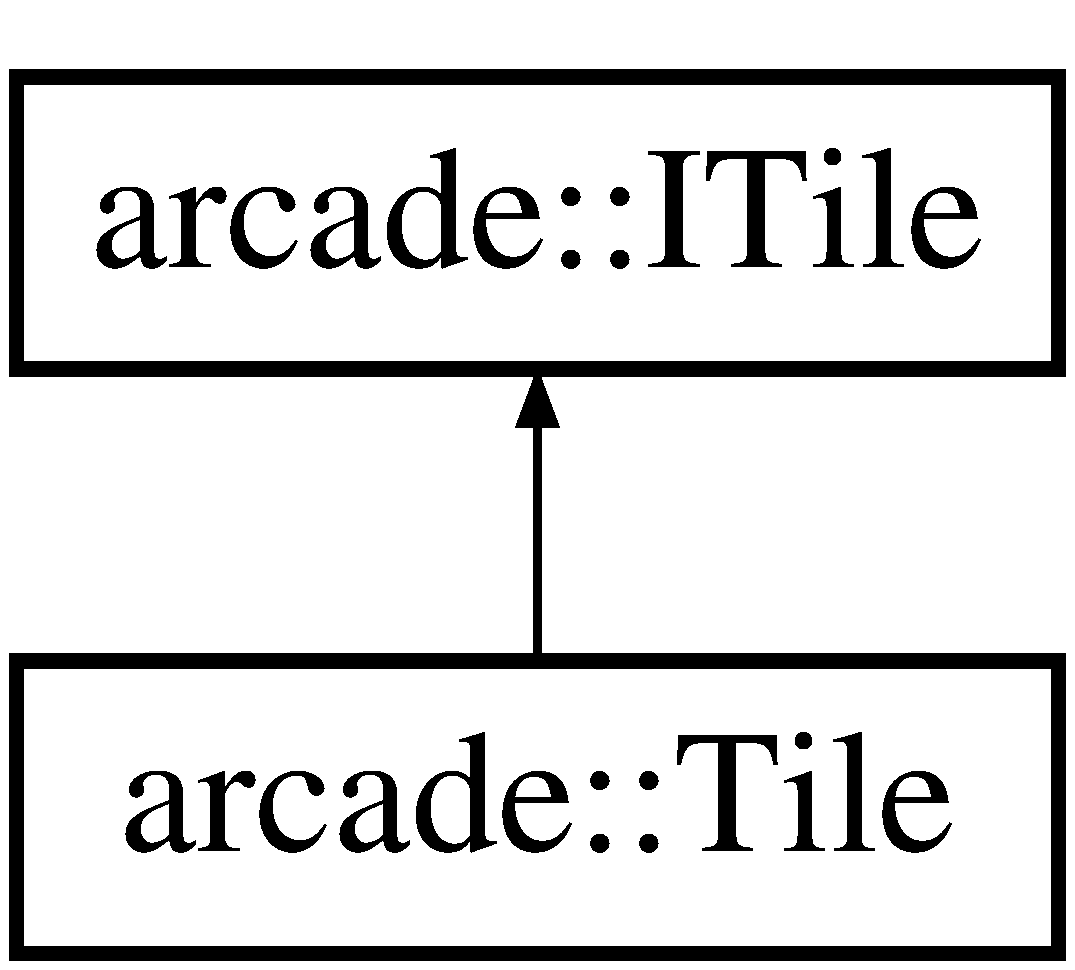
\includegraphics[height=2.000000cm]{classarcade_1_1_tile}
\end{center}
\end{figure}
\subsection*{Public Member Functions}
\begin{DoxyCompactItemize}
\item 
virtual \hyperlink{classarcade_1_1_tile_a38f5ed9f2ae16dbd42fa736ed5c984a6}{$\sim$\+Tile} ()
\item 
\hyperlink{classarcade_1_1_tile_abdc042c12eb8996f38a883c38c98efc6}{Tile} (\hyperlink{namespacearcade_a61ba576694ea309cdf2b4b66902408ca}{Tile\+Type} type)
\item 
\hyperlink{namespacearcade_a61ba576694ea309cdf2b4b66902408ca}{Tile\+Type} \hyperlink{classarcade_1_1_tile_a41277c86970f33f4a5a45d1e3233c45c}{get\+Type} () const
\item 
void \hyperlink{classarcade_1_1_tile_aefde0ece0a81584556ad5fdb17bb08a4}{set\+Type} (\hyperlink{namespacearcade_a61ba576694ea309cdf2b4b66902408ca}{Tile\+Type} type)
\item 
\hyperlink{namespacearcade_a2e0a64a64203f78c9efb84a1475a8cf4}{Tile\+Type\+Evolution} \hyperlink{classarcade_1_1_tile_a26e592479e0feb1ea584b3e96cb22ea4}{get\+Type\+Ev} () const
\item 
void \hyperlink{classarcade_1_1_tile_adac2e5710cd7651df15c33ba9aaa990f}{set\+Type\+Ev} (\hyperlink{namespacearcade_a2e0a64a64203f78c9efb84a1475a8cf4}{Tile\+Type\+Evolution} type)
\item 
\hyperlink{unionarcade_1_1_color}{Color} \hyperlink{classarcade_1_1_tile_a33f158dcb0b991ca565562a41ede70ba}{get\+Color} () const override
\begin{DoxyCompactList}\small\item\em Get the color of the tile. \end{DoxyCompactList}\item 
void \hyperlink{classarcade_1_1_tile_a07d360acc6d893cc23f972cf9bdb9c8c}{set\+Color} (union \hyperlink{unionarcade_1_1_color}{Color} color)
\item 
size\+\_\+t \hyperlink{classarcade_1_1_tile_afe2b3e7b4a6880b03772c240a2122d16}{get\+Sprite\+Id} () const override
\begin{DoxyCompactList}\small\item\em Get the sprite ID (0 if none) \end{DoxyCompactList}\item 
size\+\_\+t \hyperlink{classarcade_1_1_tile_a0dfe91e5896b8cfc3afac522d901be0a}{get\+Sprite\+Pos} () const override
\begin{DoxyCompactList}\small\item\em Get the sprite position in it\textquotesingle{}s animation. \end{DoxyCompactList}\item 
bool \hyperlink{classarcade_1_1_tile_abb9bfea961e713a36213627d0787aae2}{has\+Sprite} () const override
\begin{DoxyCompactList}\small\item\em Returns if the \hyperlink{classarcade_1_1_tile}{Tile} has a sprite affected, if not, use \hyperlink{classarcade_1_1_tile_a33f158dcb0b991ca565562a41ede70ba}{get\+Color()} \end{DoxyCompactList}\item 
double \hyperlink{classarcade_1_1_tile_a0db817dd3b7e0872e90d703bfea16005}{get\+ShiftX} () const override
\begin{DoxyCompactList}\small\item\em Get the tile position shift on x. \end{DoxyCompactList}\item 
double \hyperlink{classarcade_1_1_tile_aa28fe418563d90bd65e1c58510d28eef}{get\+ShiftY} () const override
\begin{DoxyCompactList}\small\item\em Get the tile position shift on y. \end{DoxyCompactList}\item 
void \hyperlink{classarcade_1_1_tile_a6fbee0e9aec15f1ee8b723776d67d2b4}{set\+Sprite} (int id)
\item 
void \hyperlink{classarcade_1_1_tile_a47d0874b2b1f02719574d1cae49e7a05}{remove\+Sprite} ()
\end{DoxyCompactItemize}


\subsection{Constructor \& Destructor Documentation}
\mbox{\Hypertarget{classarcade_1_1_tile_a38f5ed9f2ae16dbd42fa736ed5c984a6}\label{classarcade_1_1_tile_a38f5ed9f2ae16dbd42fa736ed5c984a6}} 
\index{arcade\+::\+Tile@{arcade\+::\+Tile}!````~Tile@{$\sim$\+Tile}}
\index{````~Tile@{$\sim$\+Tile}!arcade\+::\+Tile@{arcade\+::\+Tile}}
\subsubsection{\texorpdfstring{$\sim$\+Tile()}{~Tile()}}
{\footnotesize\ttfamily arcade\+::\+Tile\+::$\sim$\+Tile (\begin{DoxyParamCaption}{ }\end{DoxyParamCaption})\hspace{0.3cm}{\ttfamily [virtual]}}

\mbox{\Hypertarget{classarcade_1_1_tile_abdc042c12eb8996f38a883c38c98efc6}\label{classarcade_1_1_tile_abdc042c12eb8996f38a883c38c98efc6}} 
\index{arcade\+::\+Tile@{arcade\+::\+Tile}!Tile@{Tile}}
\index{Tile@{Tile}!arcade\+::\+Tile@{arcade\+::\+Tile}}
\subsubsection{\texorpdfstring{Tile()}{Tile()}}
{\footnotesize\ttfamily arcade\+::\+Tile\+::\+Tile (\begin{DoxyParamCaption}\item[{\hyperlink{namespacearcade_a61ba576694ea309cdf2b4b66902408ca}{Tile\+Type}}]{type }\end{DoxyParamCaption})}



\subsection{Member Function Documentation}
\mbox{\Hypertarget{classarcade_1_1_tile_a33f158dcb0b991ca565562a41ede70ba}\label{classarcade_1_1_tile_a33f158dcb0b991ca565562a41ede70ba}} 
\index{arcade\+::\+Tile@{arcade\+::\+Tile}!get\+Color@{get\+Color}}
\index{get\+Color@{get\+Color}!arcade\+::\+Tile@{arcade\+::\+Tile}}
\subsubsection{\texorpdfstring{get\+Color()}{getColor()}}
{\footnotesize\ttfamily \hyperlink{unionarcade_1_1_color}{arcade\+::\+Color} arcade\+::\+Tile\+::get\+Color (\begin{DoxyParamCaption}{ }\end{DoxyParamCaption}) const\hspace{0.3cm}{\ttfamily [override]}, {\ttfamily [virtual]}}



Get the color of the tile. 



Implements \hyperlink{classarcade_1_1_i_tile_adb20cb553bc2ce17dc23125eb70b8329}{arcade\+::\+I\+Tile}.

\mbox{\Hypertarget{classarcade_1_1_tile_a0db817dd3b7e0872e90d703bfea16005}\label{classarcade_1_1_tile_a0db817dd3b7e0872e90d703bfea16005}} 
\index{arcade\+::\+Tile@{arcade\+::\+Tile}!get\+ShiftX@{get\+ShiftX}}
\index{get\+ShiftX@{get\+ShiftX}!arcade\+::\+Tile@{arcade\+::\+Tile}}
\subsubsection{\texorpdfstring{get\+Shift\+X()}{getShiftX()}}
{\footnotesize\ttfamily double arcade\+::\+Tile\+::get\+ShiftX (\begin{DoxyParamCaption}{ }\end{DoxyParamCaption}) const\hspace{0.3cm}{\ttfamily [override]}, {\ttfamily [virtual]}}



Get the tile position shift on x. 



Implements \hyperlink{classarcade_1_1_i_tile_aaa83bd96759c2c9f369be4b00b8a72d2}{arcade\+::\+I\+Tile}.

\mbox{\Hypertarget{classarcade_1_1_tile_aa28fe418563d90bd65e1c58510d28eef}\label{classarcade_1_1_tile_aa28fe418563d90bd65e1c58510d28eef}} 
\index{arcade\+::\+Tile@{arcade\+::\+Tile}!get\+ShiftY@{get\+ShiftY}}
\index{get\+ShiftY@{get\+ShiftY}!arcade\+::\+Tile@{arcade\+::\+Tile}}
\subsubsection{\texorpdfstring{get\+Shift\+Y()}{getShiftY()}}
{\footnotesize\ttfamily double arcade\+::\+Tile\+::get\+ShiftY (\begin{DoxyParamCaption}{ }\end{DoxyParamCaption}) const\hspace{0.3cm}{\ttfamily [override]}, {\ttfamily [virtual]}}



Get the tile position shift on y. 



Implements \hyperlink{classarcade_1_1_i_tile_af7ca3cfb598eda00ac5b5f15f096e32f}{arcade\+::\+I\+Tile}.

\mbox{\Hypertarget{classarcade_1_1_tile_afe2b3e7b4a6880b03772c240a2122d16}\label{classarcade_1_1_tile_afe2b3e7b4a6880b03772c240a2122d16}} 
\index{arcade\+::\+Tile@{arcade\+::\+Tile}!get\+Sprite\+Id@{get\+Sprite\+Id}}
\index{get\+Sprite\+Id@{get\+Sprite\+Id}!arcade\+::\+Tile@{arcade\+::\+Tile}}
\subsubsection{\texorpdfstring{get\+Sprite\+Id()}{getSpriteId()}}
{\footnotesize\ttfamily size\+\_\+t arcade\+::\+Tile\+::get\+Sprite\+Id (\begin{DoxyParamCaption}{ }\end{DoxyParamCaption}) const\hspace{0.3cm}{\ttfamily [override]}, {\ttfamily [virtual]}}



Get the sprite ID (0 if none) 



Implements \hyperlink{classarcade_1_1_i_tile_a4c09e2ac12d75fe12e3d4d1ca4e08150}{arcade\+::\+I\+Tile}.

\mbox{\Hypertarget{classarcade_1_1_tile_a0dfe91e5896b8cfc3afac522d901be0a}\label{classarcade_1_1_tile_a0dfe91e5896b8cfc3afac522d901be0a}} 
\index{arcade\+::\+Tile@{arcade\+::\+Tile}!get\+Sprite\+Pos@{get\+Sprite\+Pos}}
\index{get\+Sprite\+Pos@{get\+Sprite\+Pos}!arcade\+::\+Tile@{arcade\+::\+Tile}}
\subsubsection{\texorpdfstring{get\+Sprite\+Pos()}{getSpritePos()}}
{\footnotesize\ttfamily size\+\_\+t arcade\+::\+Tile\+::get\+Sprite\+Pos (\begin{DoxyParamCaption}{ }\end{DoxyParamCaption}) const\hspace{0.3cm}{\ttfamily [override]}, {\ttfamily [virtual]}}



Get the sprite position in it\textquotesingle{}s animation. 



Implements \hyperlink{classarcade_1_1_i_tile_a3e5cec4407ef6afb7e10d82fb1c93f5e}{arcade\+::\+I\+Tile}.

\mbox{\Hypertarget{classarcade_1_1_tile_a41277c86970f33f4a5a45d1e3233c45c}\label{classarcade_1_1_tile_a41277c86970f33f4a5a45d1e3233c45c}} 
\index{arcade\+::\+Tile@{arcade\+::\+Tile}!get\+Type@{get\+Type}}
\index{get\+Type@{get\+Type}!arcade\+::\+Tile@{arcade\+::\+Tile}}
\subsubsection{\texorpdfstring{get\+Type()}{getType()}}
{\footnotesize\ttfamily \hyperlink{namespacearcade_a61ba576694ea309cdf2b4b66902408ca}{arcade\+::\+Tile\+Type} arcade\+::\+Tile\+::get\+Type (\begin{DoxyParamCaption}{ }\end{DoxyParamCaption}) const}

\mbox{\Hypertarget{classarcade_1_1_tile_a26e592479e0feb1ea584b3e96cb22ea4}\label{classarcade_1_1_tile_a26e592479e0feb1ea584b3e96cb22ea4}} 
\index{arcade\+::\+Tile@{arcade\+::\+Tile}!get\+Type\+Ev@{get\+Type\+Ev}}
\index{get\+Type\+Ev@{get\+Type\+Ev}!arcade\+::\+Tile@{arcade\+::\+Tile}}
\subsubsection{\texorpdfstring{get\+Type\+Ev()}{getTypeEv()}}
{\footnotesize\ttfamily \hyperlink{namespacearcade_a2e0a64a64203f78c9efb84a1475a8cf4}{arcade\+::\+Tile\+Type\+Evolution} arcade\+::\+Tile\+::get\+Type\+Ev (\begin{DoxyParamCaption}{ }\end{DoxyParamCaption}) const}

\mbox{\Hypertarget{classarcade_1_1_tile_abb9bfea961e713a36213627d0787aae2}\label{classarcade_1_1_tile_abb9bfea961e713a36213627d0787aae2}} 
\index{arcade\+::\+Tile@{arcade\+::\+Tile}!has\+Sprite@{has\+Sprite}}
\index{has\+Sprite@{has\+Sprite}!arcade\+::\+Tile@{arcade\+::\+Tile}}
\subsubsection{\texorpdfstring{has\+Sprite()}{hasSprite()}}
{\footnotesize\ttfamily bool arcade\+::\+Tile\+::has\+Sprite (\begin{DoxyParamCaption}{ }\end{DoxyParamCaption}) const\hspace{0.3cm}{\ttfamily [override]}, {\ttfamily [virtual]}}



Returns if the \hyperlink{classarcade_1_1_tile}{Tile} has a sprite affected, if not, use \hyperlink{classarcade_1_1_tile_a33f158dcb0b991ca565562a41ede70ba}{get\+Color()} 



Implements \hyperlink{classarcade_1_1_i_tile_ab2d6a5f8d4cfc6c606b8ad13d8dd88a4}{arcade\+::\+I\+Tile}.

\mbox{\Hypertarget{classarcade_1_1_tile_a47d0874b2b1f02719574d1cae49e7a05}\label{classarcade_1_1_tile_a47d0874b2b1f02719574d1cae49e7a05}} 
\index{arcade\+::\+Tile@{arcade\+::\+Tile}!remove\+Sprite@{remove\+Sprite}}
\index{remove\+Sprite@{remove\+Sprite}!arcade\+::\+Tile@{arcade\+::\+Tile}}
\subsubsection{\texorpdfstring{remove\+Sprite()}{removeSprite()}}
{\footnotesize\ttfamily void arcade\+::\+Tile\+::remove\+Sprite (\begin{DoxyParamCaption}{ }\end{DoxyParamCaption})}

\mbox{\Hypertarget{classarcade_1_1_tile_a07d360acc6d893cc23f972cf9bdb9c8c}\label{classarcade_1_1_tile_a07d360acc6d893cc23f972cf9bdb9c8c}} 
\index{arcade\+::\+Tile@{arcade\+::\+Tile}!set\+Color@{set\+Color}}
\index{set\+Color@{set\+Color}!arcade\+::\+Tile@{arcade\+::\+Tile}}
\subsubsection{\texorpdfstring{set\+Color()}{setColor()}}
{\footnotesize\ttfamily void arcade\+::\+Tile\+::set\+Color (\begin{DoxyParamCaption}\item[{union \hyperlink{unionarcade_1_1_color}{Color}}]{color }\end{DoxyParamCaption})}

\mbox{\Hypertarget{classarcade_1_1_tile_a6fbee0e9aec15f1ee8b723776d67d2b4}\label{classarcade_1_1_tile_a6fbee0e9aec15f1ee8b723776d67d2b4}} 
\index{arcade\+::\+Tile@{arcade\+::\+Tile}!set\+Sprite@{set\+Sprite}}
\index{set\+Sprite@{set\+Sprite}!arcade\+::\+Tile@{arcade\+::\+Tile}}
\subsubsection{\texorpdfstring{set\+Sprite()}{setSprite()}}
{\footnotesize\ttfamily void arcade\+::\+Tile\+::set\+Sprite (\begin{DoxyParamCaption}\item[{int}]{id }\end{DoxyParamCaption})}

\mbox{\Hypertarget{classarcade_1_1_tile_aefde0ece0a81584556ad5fdb17bb08a4}\label{classarcade_1_1_tile_aefde0ece0a81584556ad5fdb17bb08a4}} 
\index{arcade\+::\+Tile@{arcade\+::\+Tile}!set\+Type@{set\+Type}}
\index{set\+Type@{set\+Type}!arcade\+::\+Tile@{arcade\+::\+Tile}}
\subsubsection{\texorpdfstring{set\+Type()}{setType()}}
{\footnotesize\ttfamily void arcade\+::\+Tile\+::set\+Type (\begin{DoxyParamCaption}\item[{\hyperlink{namespacearcade_a61ba576694ea309cdf2b4b66902408ca}{arcade\+::\+Tile\+Type}}]{type }\end{DoxyParamCaption})}

\mbox{\Hypertarget{classarcade_1_1_tile_adac2e5710cd7651df15c33ba9aaa990f}\label{classarcade_1_1_tile_adac2e5710cd7651df15c33ba9aaa990f}} 
\index{arcade\+::\+Tile@{arcade\+::\+Tile}!set\+Type\+Ev@{set\+Type\+Ev}}
\index{set\+Type\+Ev@{set\+Type\+Ev}!arcade\+::\+Tile@{arcade\+::\+Tile}}
\subsubsection{\texorpdfstring{set\+Type\+Ev()}{setTypeEv()}}
{\footnotesize\ttfamily void arcade\+::\+Tile\+::set\+Type\+Ev (\begin{DoxyParamCaption}\item[{\hyperlink{namespacearcade_a2e0a64a64203f78c9efb84a1475a8cf4}{Tile\+Type\+Evolution}}]{type }\end{DoxyParamCaption})}



The documentation for this class was generated from the following files\+:\begin{DoxyCompactItemize}
\item 
include/\hyperlink{_tile_8hpp}{Tile.\+hpp}\item 
srcs/\hyperlink{_tile_8cpp}{Tile.\+cpp}\end{DoxyCompactItemize}

\hypertarget{class_timer}{}\section{Timer Class Reference}
\label{class_timer}\index{Timer@{Timer}}


{\ttfamily \#include $<$Timer.\+hpp$>$}

\subsection*{Public Member Functions}
\begin{DoxyCompactItemize}
\item 
virtual \hyperlink{class_timer_a14fa469c4c295c5fa6e66a4ad1092146}{$\sim$\+Timer} ()
\item 
\hyperlink{class_timer_a5f16e8da27d2a5a5242dead46de05d97}{Timer} ()
\item 
void \hyperlink{class_timer_a3a8b5272198d029779dc9302a54305a8}{start} ()
\item 
std\+::chrono\+::steady\+\_\+clock\+::duration \hyperlink{class_timer_a2ddb5fe1533752992785fb06e86b7c07}{time\+Elapsed} () const
\item 
long \hyperlink{class_timer_aee5dbd672b676eed86a5594f7072719e}{time\+Elapsed\+Milliseconds} () const
\item 
long \hyperlink{class_timer_ad15a9b6eff0680b58675e52a3959cb1d}{time\+Elapsed\+Seconds} () const
\item 
bool \hyperlink{class_timer_ab12a809d6520150d9eeec6b5f5511854}{is\+Time\+Over\+Milliseconds} (double milliseconds)
\item 
bool \hyperlink{class_timer_a99830a54e401b61cdf0777940f6e36e7}{is\+Time\+Over\+Seconds} (double seconds)
\end{DoxyCompactItemize}


\subsection{Constructor \& Destructor Documentation}
\mbox{\Hypertarget{class_timer_a14fa469c4c295c5fa6e66a4ad1092146}\label{class_timer_a14fa469c4c295c5fa6e66a4ad1092146}} 
\index{Timer@{Timer}!````~Timer@{$\sim$\+Timer}}
\index{````~Timer@{$\sim$\+Timer}!Timer@{Timer}}
\subsubsection{\texorpdfstring{$\sim$\+Timer()}{~Timer()}}
{\footnotesize\ttfamily Timer\+::$\sim$\+Timer (\begin{DoxyParamCaption}{ }\end{DoxyParamCaption})\hspace{0.3cm}{\ttfamily [virtual]}}

\mbox{\Hypertarget{class_timer_a5f16e8da27d2a5a5242dead46de05d97}\label{class_timer_a5f16e8da27d2a5a5242dead46de05d97}} 
\index{Timer@{Timer}!Timer@{Timer}}
\index{Timer@{Timer}!Timer@{Timer}}
\subsubsection{\texorpdfstring{Timer()}{Timer()}}
{\footnotesize\ttfamily Timer\+::\+Timer (\begin{DoxyParamCaption}{ }\end{DoxyParamCaption})}



\subsection{Member Function Documentation}
\mbox{\Hypertarget{class_timer_ab12a809d6520150d9eeec6b5f5511854}\label{class_timer_ab12a809d6520150d9eeec6b5f5511854}} 
\index{Timer@{Timer}!is\+Time\+Over\+Milliseconds@{is\+Time\+Over\+Milliseconds}}
\index{is\+Time\+Over\+Milliseconds@{is\+Time\+Over\+Milliseconds}!Timer@{Timer}}
\subsubsection{\texorpdfstring{is\+Time\+Over\+Milliseconds()}{isTimeOverMilliseconds()}}
{\footnotesize\ttfamily bool Timer\+::is\+Time\+Over\+Milliseconds (\begin{DoxyParamCaption}\item[{double}]{milliseconds }\end{DoxyParamCaption})}

\mbox{\Hypertarget{class_timer_a99830a54e401b61cdf0777940f6e36e7}\label{class_timer_a99830a54e401b61cdf0777940f6e36e7}} 
\index{Timer@{Timer}!is\+Time\+Over\+Seconds@{is\+Time\+Over\+Seconds}}
\index{is\+Time\+Over\+Seconds@{is\+Time\+Over\+Seconds}!Timer@{Timer}}
\subsubsection{\texorpdfstring{is\+Time\+Over\+Seconds()}{isTimeOverSeconds()}}
{\footnotesize\ttfamily bool Timer\+::is\+Time\+Over\+Seconds (\begin{DoxyParamCaption}\item[{double}]{seconds }\end{DoxyParamCaption})}

\mbox{\Hypertarget{class_timer_a3a8b5272198d029779dc9302a54305a8}\label{class_timer_a3a8b5272198d029779dc9302a54305a8}} 
\index{Timer@{Timer}!start@{start}}
\index{start@{start}!Timer@{Timer}}
\subsubsection{\texorpdfstring{start()}{start()}}
{\footnotesize\ttfamily void Timer\+::start (\begin{DoxyParamCaption}{ }\end{DoxyParamCaption})}

\mbox{\Hypertarget{class_timer_a2ddb5fe1533752992785fb06e86b7c07}\label{class_timer_a2ddb5fe1533752992785fb06e86b7c07}} 
\index{Timer@{Timer}!time\+Elapsed@{time\+Elapsed}}
\index{time\+Elapsed@{time\+Elapsed}!Timer@{Timer}}
\subsubsection{\texorpdfstring{time\+Elapsed()}{timeElapsed()}}
{\footnotesize\ttfamily std\+::chrono\+::steady\+\_\+clock\+::duration Timer\+::time\+Elapsed (\begin{DoxyParamCaption}{ }\end{DoxyParamCaption}) const}

\mbox{\Hypertarget{class_timer_aee5dbd672b676eed86a5594f7072719e}\label{class_timer_aee5dbd672b676eed86a5594f7072719e}} 
\index{Timer@{Timer}!time\+Elapsed\+Milliseconds@{time\+Elapsed\+Milliseconds}}
\index{time\+Elapsed\+Milliseconds@{time\+Elapsed\+Milliseconds}!Timer@{Timer}}
\subsubsection{\texorpdfstring{time\+Elapsed\+Milliseconds()}{timeElapsedMilliseconds()}}
{\footnotesize\ttfamily long Timer\+::time\+Elapsed\+Milliseconds (\begin{DoxyParamCaption}{ }\end{DoxyParamCaption}) const}

\mbox{\Hypertarget{class_timer_ad15a9b6eff0680b58675e52a3959cb1d}\label{class_timer_ad15a9b6eff0680b58675e52a3959cb1d}} 
\index{Timer@{Timer}!time\+Elapsed\+Seconds@{time\+Elapsed\+Seconds}}
\index{time\+Elapsed\+Seconds@{time\+Elapsed\+Seconds}!Timer@{Timer}}
\subsubsection{\texorpdfstring{time\+Elapsed\+Seconds()}{timeElapsedSeconds()}}
{\footnotesize\ttfamily long Timer\+::time\+Elapsed\+Seconds (\begin{DoxyParamCaption}{ }\end{DoxyParamCaption}) const}



The documentation for this class was generated from the following files\+:\begin{DoxyCompactItemize}
\item 
include/\hyperlink{_timer_8hpp}{Timer.\+hpp}\item 
srcs/\hyperlink{_timer_8cpp}{Timer.\+cpp}\end{DoxyCompactItemize}

\hypertarget{classarcade_1_1_u_i_component}{}\section{arcade\+:\+:U\+I\+Component Class Reference}
\label{classarcade_1_1_u_i_component}\index{arcade\+::\+U\+I\+Component@{arcade\+::\+U\+I\+Component}}


{\ttfamily \#include $<$U\+I\+Component.\+hpp$>$}

Inheritance diagram for arcade\+:\+:U\+I\+Component\+:\begin{figure}[H]
\begin{center}
\leavevmode
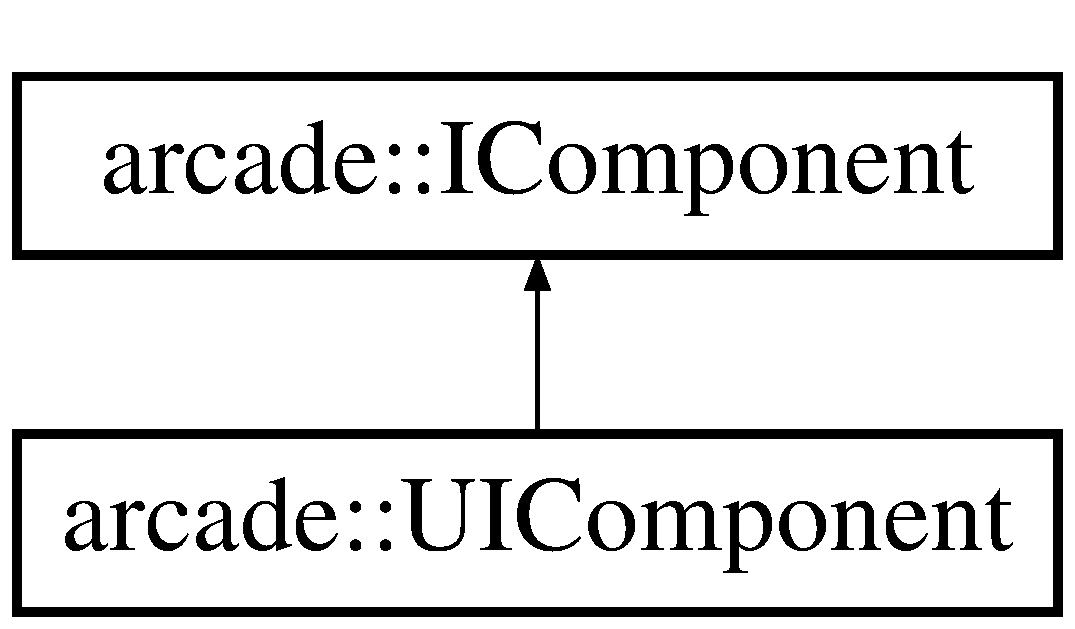
\includegraphics[height=2.000000cm]{classarcade_1_1_u_i_component}
\end{center}
\end{figure}
\subsection*{Public Member Functions}
\begin{DoxyCompactItemize}
\item 
virtual \hyperlink{classarcade_1_1_u_i_component_ac2ca5956fe64bfbdc7b1fe2e97293396}{$\sim$\+U\+I\+Component} ()
\item 
\hyperlink{classarcade_1_1_u_i_component_aa5911db06c5159c74c99175180ac265d}{U\+I\+Component} (double x, double y, double width, double height)
\item 
double \hyperlink{classarcade_1_1_u_i_component_a8da01c706810692c7c3f0711c957fb15}{getX} () const override
\begin{DoxyCompactList}\small\item\em Get the X position (between 0.\+0 and 1.\+0) \end{DoxyCompactList}\item 
double \hyperlink{classarcade_1_1_u_i_component_af5360eec3a1a473484df1df5f7d89ee9}{getY} () const override
\begin{DoxyCompactList}\small\item\em Get the Y position (between 0.\+0 and 1.\+0) \end{DoxyCompactList}\item 
double \hyperlink{classarcade_1_1_u_i_component_a56c4ce3124813be5d456aec399c63bc9}{get\+Width} () const override
\item 
double \hyperlink{classarcade_1_1_u_i_component_abb02d0b9324eabf8ddf0d1302a0b08f7}{get\+Height} () const override
\begin{DoxyCompactList}\small\item\em Get the component\textquotesingle{}s height (between 0.\+0 and 1.\+0) \end{DoxyCompactList}\item 
size\+\_\+t \hyperlink{classarcade_1_1_u_i_component_a7da87b1ce3bc56dcc6600e1c27e325a6}{get\+Background\+Id} () const override
\begin{DoxyCompactList}\small\item\em Get the id of the background sprite. \end{DoxyCompactList}\item 
\hyperlink{unionarcade_1_1_color}{Color} \hyperlink{classarcade_1_1_u_i_component_a981bbd394540b39ca0c7c0f760ef9551}{get\+Background\+Color} () const override
\begin{DoxyCompactList}\small\item\em Get the color of the background. \end{DoxyCompactList}\item 
void \hyperlink{classarcade_1_1_u_i_component_abf7a2ca878ba0963e2c3ac17207f0622}{set\+Text} (const std\+::string \&text)
\item 
void \hyperlink{classarcade_1_1_u_i_component_a9adbc1ec26ce4d5e707b975026f4e499}{set\+Bg\+Color} (const \hyperlink{unionarcade_1_1_color}{Color} \&bg\+Color)
\item 
void \hyperlink{classarcade_1_1_u_i_component_abaab3b3d90da61e7a579b57f2cf3c35e}{set\+Text\+Color} (const \hyperlink{unionarcade_1_1_color}{Color} \&text\+Color)
\item 
const std\+::string \& \hyperlink{classarcade_1_1_u_i_component_aa930897f9456ed9462063481d19d10ed}{get\+Text} () const override
\begin{DoxyCompactList}\small\item\em Get the text value. \end{DoxyCompactList}\item 
bool \hyperlink{classarcade_1_1_u_i_component_a0f41ff1be1ae457a3be0856553e904f4}{has\+Sprite} () const override
\begin{DoxyCompactList}\small\item\em Return true if the component has a sprite. \end{DoxyCompactList}\item 
\hyperlink{unionarcade_1_1_color}{Color} \hyperlink{classarcade_1_1_u_i_component_a0a9e2a34357ad6759d580e152a20adee}{get\+Text\+Color} () const override
\item 
void \hyperlink{classarcade_1_1_u_i_component_a8d87597d38fbc7cd93835d5712e3915c}{set\+Clicked} () override
\begin{DoxyCompactList}\small\item\em Way of the lib to tell a component it was clicked. \end{DoxyCompactList}\item 
bool \hyperlink{classarcade_1_1_u_i_component_a3ee6eaf72f0622ac5e49c285b48d73a6}{is\+Hover} () const
\item 
void \hyperlink{classarcade_1_1_u_i_component_a08ab8e887fe7f5337ac0e87a82105e37}{set\+Hover} (bool hover)
\item 
bool \hyperlink{classarcade_1_1_u_i_component_ad1ee9ac6cbe4dfd28e399317c5d38e8c}{is\+Selected} () const
\item 
void \hyperlink{classarcade_1_1_u_i_component_aa09f60dbf12dcb42e15b7a23ae61bf74}{set\+Selected} (bool selected)
\item 
void \hyperlink{classarcade_1_1_u_i_component_a055dcadcb7799e09fa9aa29c9e1b8f48}{toogle} ()
\end{DoxyCompactItemize}


\subsection{Constructor \& Destructor Documentation}
\mbox{\Hypertarget{classarcade_1_1_u_i_component_ac2ca5956fe64bfbdc7b1fe2e97293396}\label{classarcade_1_1_u_i_component_ac2ca5956fe64bfbdc7b1fe2e97293396}} 
\index{arcade\+::\+U\+I\+Component@{arcade\+::\+U\+I\+Component}!````~U\+I\+Component@{$\sim$\+U\+I\+Component}}
\index{````~U\+I\+Component@{$\sim$\+U\+I\+Component}!arcade\+::\+U\+I\+Component@{arcade\+::\+U\+I\+Component}}
\subsubsection{\texorpdfstring{$\sim$\+U\+I\+Component()}{~UIComponent()}}
{\footnotesize\ttfamily arcade\+::\+U\+I\+Component\+::$\sim$\+U\+I\+Component (\begin{DoxyParamCaption}{ }\end{DoxyParamCaption})\hspace{0.3cm}{\ttfamily [virtual]}}

\mbox{\Hypertarget{classarcade_1_1_u_i_component_aa5911db06c5159c74c99175180ac265d}\label{classarcade_1_1_u_i_component_aa5911db06c5159c74c99175180ac265d}} 
\index{arcade\+::\+U\+I\+Component@{arcade\+::\+U\+I\+Component}!U\+I\+Component@{U\+I\+Component}}
\index{U\+I\+Component@{U\+I\+Component}!arcade\+::\+U\+I\+Component@{arcade\+::\+U\+I\+Component}}
\subsubsection{\texorpdfstring{U\+I\+Component()}{UIComponent()}}
{\footnotesize\ttfamily arcade\+::\+U\+I\+Component\+::\+U\+I\+Component (\begin{DoxyParamCaption}\item[{double}]{x,  }\item[{double}]{y,  }\item[{double}]{width,  }\item[{double}]{height }\end{DoxyParamCaption})}



\subsection{Member Function Documentation}
\mbox{\Hypertarget{classarcade_1_1_u_i_component_a981bbd394540b39ca0c7c0f760ef9551}\label{classarcade_1_1_u_i_component_a981bbd394540b39ca0c7c0f760ef9551}} 
\index{arcade\+::\+U\+I\+Component@{arcade\+::\+U\+I\+Component}!get\+Background\+Color@{get\+Background\+Color}}
\index{get\+Background\+Color@{get\+Background\+Color}!arcade\+::\+U\+I\+Component@{arcade\+::\+U\+I\+Component}}
\subsubsection{\texorpdfstring{get\+Background\+Color()}{getBackgroundColor()}}
{\footnotesize\ttfamily \hyperlink{unionarcade_1_1_color}{arcade\+::\+Color} arcade\+::\+U\+I\+Component\+::get\+Background\+Color (\begin{DoxyParamCaption}{ }\end{DoxyParamCaption}) const\hspace{0.3cm}{\ttfamily [override]}, {\ttfamily [virtual]}}



Get the color of the background. 



Implements \hyperlink{classarcade_1_1_i_component_a99301c61be2a21ef8a274727ba781a00}{arcade\+::\+I\+Component}.

\mbox{\Hypertarget{classarcade_1_1_u_i_component_a7da87b1ce3bc56dcc6600e1c27e325a6}\label{classarcade_1_1_u_i_component_a7da87b1ce3bc56dcc6600e1c27e325a6}} 
\index{arcade\+::\+U\+I\+Component@{arcade\+::\+U\+I\+Component}!get\+Background\+Id@{get\+Background\+Id}}
\index{get\+Background\+Id@{get\+Background\+Id}!arcade\+::\+U\+I\+Component@{arcade\+::\+U\+I\+Component}}
\subsubsection{\texorpdfstring{get\+Background\+Id()}{getBackgroundId()}}
{\footnotesize\ttfamily size\+\_\+t arcade\+::\+U\+I\+Component\+::get\+Background\+Id (\begin{DoxyParamCaption}{ }\end{DoxyParamCaption}) const\hspace{0.3cm}{\ttfamily [override]}, {\ttfamily [virtual]}}



Get the id of the background sprite. 



Implements \hyperlink{classarcade_1_1_i_component_a7d4c00172b0ba0e3dc63832a9234efbb}{arcade\+::\+I\+Component}.

\mbox{\Hypertarget{classarcade_1_1_u_i_component_abb02d0b9324eabf8ddf0d1302a0b08f7}\label{classarcade_1_1_u_i_component_abb02d0b9324eabf8ddf0d1302a0b08f7}} 
\index{arcade\+::\+U\+I\+Component@{arcade\+::\+U\+I\+Component}!get\+Height@{get\+Height}}
\index{get\+Height@{get\+Height}!arcade\+::\+U\+I\+Component@{arcade\+::\+U\+I\+Component}}
\subsubsection{\texorpdfstring{get\+Height()}{getHeight()}}
{\footnotesize\ttfamily double arcade\+::\+U\+I\+Component\+::get\+Height (\begin{DoxyParamCaption}{ }\end{DoxyParamCaption}) const\hspace{0.3cm}{\ttfamily [override]}, {\ttfamily [virtual]}}



Get the component\textquotesingle{}s height (between 0.\+0 and 1.\+0) 



Implements \hyperlink{classarcade_1_1_i_component_a77a3bed39227f11d06bb71e06ee2ee30}{arcade\+::\+I\+Component}.

\mbox{\Hypertarget{classarcade_1_1_u_i_component_aa930897f9456ed9462063481d19d10ed}\label{classarcade_1_1_u_i_component_aa930897f9456ed9462063481d19d10ed}} 
\index{arcade\+::\+U\+I\+Component@{arcade\+::\+U\+I\+Component}!get\+Text@{get\+Text}}
\index{get\+Text@{get\+Text}!arcade\+::\+U\+I\+Component@{arcade\+::\+U\+I\+Component}}
\subsubsection{\texorpdfstring{get\+Text()}{getText()}}
{\footnotesize\ttfamily const std\+::string \& arcade\+::\+U\+I\+Component\+::get\+Text (\begin{DoxyParamCaption}{ }\end{DoxyParamCaption}) const\hspace{0.3cm}{\ttfamily [override]}, {\ttfamily [virtual]}}



Get the text value. 



Implements \hyperlink{classarcade_1_1_i_component_a7c09ef60e3d41d4afedf2be77fe880a7}{arcade\+::\+I\+Component}.

\mbox{\Hypertarget{classarcade_1_1_u_i_component_a0a9e2a34357ad6759d580e152a20adee}\label{classarcade_1_1_u_i_component_a0a9e2a34357ad6759d580e152a20adee}} 
\index{arcade\+::\+U\+I\+Component@{arcade\+::\+U\+I\+Component}!get\+Text\+Color@{get\+Text\+Color}}
\index{get\+Text\+Color@{get\+Text\+Color}!arcade\+::\+U\+I\+Component@{arcade\+::\+U\+I\+Component}}
\subsubsection{\texorpdfstring{get\+Text\+Color()}{getTextColor()}}
{\footnotesize\ttfamily \hyperlink{unionarcade_1_1_color}{arcade\+::\+Color} arcade\+::\+U\+I\+Component\+::get\+Text\+Color (\begin{DoxyParamCaption}{ }\end{DoxyParamCaption}) const\hspace{0.3cm}{\ttfamily [override]}, {\ttfamily [virtual]}}



Implements \hyperlink{classarcade_1_1_i_component_a9d4c57ad7c49e39ef0269f10fdc14807}{arcade\+::\+I\+Component}.

\mbox{\Hypertarget{classarcade_1_1_u_i_component_a56c4ce3124813be5d456aec399c63bc9}\label{classarcade_1_1_u_i_component_a56c4ce3124813be5d456aec399c63bc9}} 
\index{arcade\+::\+U\+I\+Component@{arcade\+::\+U\+I\+Component}!get\+Width@{get\+Width}}
\index{get\+Width@{get\+Width}!arcade\+::\+U\+I\+Component@{arcade\+::\+U\+I\+Component}}
\subsubsection{\texorpdfstring{get\+Width()}{getWidth()}}
{\footnotesize\ttfamily double arcade\+::\+U\+I\+Component\+::get\+Width (\begin{DoxyParamCaption}{ }\end{DoxyParamCaption}) const\hspace{0.3cm}{\ttfamily [override]}, {\ttfamily [virtual]}}



Implements \hyperlink{classarcade_1_1_i_component_a558e5d49736a3828753a4062d5c9bfb1}{arcade\+::\+I\+Component}.

\mbox{\Hypertarget{classarcade_1_1_u_i_component_a8da01c706810692c7c3f0711c957fb15}\label{classarcade_1_1_u_i_component_a8da01c706810692c7c3f0711c957fb15}} 
\index{arcade\+::\+U\+I\+Component@{arcade\+::\+U\+I\+Component}!getX@{getX}}
\index{getX@{getX}!arcade\+::\+U\+I\+Component@{arcade\+::\+U\+I\+Component}}
\subsubsection{\texorpdfstring{get\+X()}{getX()}}
{\footnotesize\ttfamily double arcade\+::\+U\+I\+Component\+::getX (\begin{DoxyParamCaption}{ }\end{DoxyParamCaption}) const\hspace{0.3cm}{\ttfamily [override]}, {\ttfamily [virtual]}}



Get the X position (between 0.\+0 and 1.\+0) 



Implements \hyperlink{classarcade_1_1_i_component_ab9d24992e8519756d56c0282001eccce}{arcade\+::\+I\+Component}.

\mbox{\Hypertarget{classarcade_1_1_u_i_component_af5360eec3a1a473484df1df5f7d89ee9}\label{classarcade_1_1_u_i_component_af5360eec3a1a473484df1df5f7d89ee9}} 
\index{arcade\+::\+U\+I\+Component@{arcade\+::\+U\+I\+Component}!getY@{getY}}
\index{getY@{getY}!arcade\+::\+U\+I\+Component@{arcade\+::\+U\+I\+Component}}
\subsubsection{\texorpdfstring{get\+Y()}{getY()}}
{\footnotesize\ttfamily double arcade\+::\+U\+I\+Component\+::getY (\begin{DoxyParamCaption}{ }\end{DoxyParamCaption}) const\hspace{0.3cm}{\ttfamily [override]}, {\ttfamily [virtual]}}



Get the Y position (between 0.\+0 and 1.\+0) 



Implements \hyperlink{classarcade_1_1_i_component_ad19f185c30ab99ed831d2c68fabf920f}{arcade\+::\+I\+Component}.

\mbox{\Hypertarget{classarcade_1_1_u_i_component_a0f41ff1be1ae457a3be0856553e904f4}\label{classarcade_1_1_u_i_component_a0f41ff1be1ae457a3be0856553e904f4}} 
\index{arcade\+::\+U\+I\+Component@{arcade\+::\+U\+I\+Component}!has\+Sprite@{has\+Sprite}}
\index{has\+Sprite@{has\+Sprite}!arcade\+::\+U\+I\+Component@{arcade\+::\+U\+I\+Component}}
\subsubsection{\texorpdfstring{has\+Sprite()}{hasSprite()}}
{\footnotesize\ttfamily bool arcade\+::\+U\+I\+Component\+::has\+Sprite (\begin{DoxyParamCaption}{ }\end{DoxyParamCaption}) const\hspace{0.3cm}{\ttfamily [override]}, {\ttfamily [virtual]}}



Return true if the component has a sprite. 



Implements \hyperlink{classarcade_1_1_i_component_a03ea8019a23fd44731a06548ef7e6ff3}{arcade\+::\+I\+Component}.

\mbox{\Hypertarget{classarcade_1_1_u_i_component_a3ee6eaf72f0622ac5e49c285b48d73a6}\label{classarcade_1_1_u_i_component_a3ee6eaf72f0622ac5e49c285b48d73a6}} 
\index{arcade\+::\+U\+I\+Component@{arcade\+::\+U\+I\+Component}!is\+Hover@{is\+Hover}}
\index{is\+Hover@{is\+Hover}!arcade\+::\+U\+I\+Component@{arcade\+::\+U\+I\+Component}}
\subsubsection{\texorpdfstring{is\+Hover()}{isHover()}}
{\footnotesize\ttfamily bool arcade\+::\+U\+I\+Component\+::is\+Hover (\begin{DoxyParamCaption}{ }\end{DoxyParamCaption}) const}

\mbox{\Hypertarget{classarcade_1_1_u_i_component_ad1ee9ac6cbe4dfd28e399317c5d38e8c}\label{classarcade_1_1_u_i_component_ad1ee9ac6cbe4dfd28e399317c5d38e8c}} 
\index{arcade\+::\+U\+I\+Component@{arcade\+::\+U\+I\+Component}!is\+Selected@{is\+Selected}}
\index{is\+Selected@{is\+Selected}!arcade\+::\+U\+I\+Component@{arcade\+::\+U\+I\+Component}}
\subsubsection{\texorpdfstring{is\+Selected()}{isSelected()}}
{\footnotesize\ttfamily bool arcade\+::\+U\+I\+Component\+::is\+Selected (\begin{DoxyParamCaption}{ }\end{DoxyParamCaption}) const}

\mbox{\Hypertarget{classarcade_1_1_u_i_component_a9adbc1ec26ce4d5e707b975026f4e499}\label{classarcade_1_1_u_i_component_a9adbc1ec26ce4d5e707b975026f4e499}} 
\index{arcade\+::\+U\+I\+Component@{arcade\+::\+U\+I\+Component}!set\+Bg\+Color@{set\+Bg\+Color}}
\index{set\+Bg\+Color@{set\+Bg\+Color}!arcade\+::\+U\+I\+Component@{arcade\+::\+U\+I\+Component}}
\subsubsection{\texorpdfstring{set\+Bg\+Color()}{setBgColor()}}
{\footnotesize\ttfamily void arcade\+::\+U\+I\+Component\+::set\+Bg\+Color (\begin{DoxyParamCaption}\item[{const \hyperlink{unionarcade_1_1_color}{Color} \&}]{bg\+Color }\end{DoxyParamCaption})}

\mbox{\Hypertarget{classarcade_1_1_u_i_component_a8d87597d38fbc7cd93835d5712e3915c}\label{classarcade_1_1_u_i_component_a8d87597d38fbc7cd93835d5712e3915c}} 
\index{arcade\+::\+U\+I\+Component@{arcade\+::\+U\+I\+Component}!set\+Clicked@{set\+Clicked}}
\index{set\+Clicked@{set\+Clicked}!arcade\+::\+U\+I\+Component@{arcade\+::\+U\+I\+Component}}
\subsubsection{\texorpdfstring{set\+Clicked()}{setClicked()}}
{\footnotesize\ttfamily void arcade\+::\+U\+I\+Component\+::set\+Clicked (\begin{DoxyParamCaption}{ }\end{DoxyParamCaption})\hspace{0.3cm}{\ttfamily [override]}, {\ttfamily [virtual]}}



Way of the lib to tell a component it was clicked. 



Implements \hyperlink{classarcade_1_1_i_component_ae0cd9b58ad0b127c671a5d8f92d9c25f}{arcade\+::\+I\+Component}.

\mbox{\Hypertarget{classarcade_1_1_u_i_component_a08ab8e887fe7f5337ac0e87a82105e37}\label{classarcade_1_1_u_i_component_a08ab8e887fe7f5337ac0e87a82105e37}} 
\index{arcade\+::\+U\+I\+Component@{arcade\+::\+U\+I\+Component}!set\+Hover@{set\+Hover}}
\index{set\+Hover@{set\+Hover}!arcade\+::\+U\+I\+Component@{arcade\+::\+U\+I\+Component}}
\subsubsection{\texorpdfstring{set\+Hover()}{setHover()}}
{\footnotesize\ttfamily void arcade\+::\+U\+I\+Component\+::set\+Hover (\begin{DoxyParamCaption}\item[{bool}]{hover }\end{DoxyParamCaption})}

\mbox{\Hypertarget{classarcade_1_1_u_i_component_aa09f60dbf12dcb42e15b7a23ae61bf74}\label{classarcade_1_1_u_i_component_aa09f60dbf12dcb42e15b7a23ae61bf74}} 
\index{arcade\+::\+U\+I\+Component@{arcade\+::\+U\+I\+Component}!set\+Selected@{set\+Selected}}
\index{set\+Selected@{set\+Selected}!arcade\+::\+U\+I\+Component@{arcade\+::\+U\+I\+Component}}
\subsubsection{\texorpdfstring{set\+Selected()}{setSelected()}}
{\footnotesize\ttfamily void arcade\+::\+U\+I\+Component\+::set\+Selected (\begin{DoxyParamCaption}\item[{bool}]{selected }\end{DoxyParamCaption})}

\mbox{\Hypertarget{classarcade_1_1_u_i_component_abf7a2ca878ba0963e2c3ac17207f0622}\label{classarcade_1_1_u_i_component_abf7a2ca878ba0963e2c3ac17207f0622}} 
\index{arcade\+::\+U\+I\+Component@{arcade\+::\+U\+I\+Component}!set\+Text@{set\+Text}}
\index{set\+Text@{set\+Text}!arcade\+::\+U\+I\+Component@{arcade\+::\+U\+I\+Component}}
\subsubsection{\texorpdfstring{set\+Text()}{setText()}}
{\footnotesize\ttfamily void arcade\+::\+U\+I\+Component\+::set\+Text (\begin{DoxyParamCaption}\item[{const std\+::string \&}]{text }\end{DoxyParamCaption})}

\mbox{\Hypertarget{classarcade_1_1_u_i_component_abaab3b3d90da61e7a579b57f2cf3c35e}\label{classarcade_1_1_u_i_component_abaab3b3d90da61e7a579b57f2cf3c35e}} 
\index{arcade\+::\+U\+I\+Component@{arcade\+::\+U\+I\+Component}!set\+Text\+Color@{set\+Text\+Color}}
\index{set\+Text\+Color@{set\+Text\+Color}!arcade\+::\+U\+I\+Component@{arcade\+::\+U\+I\+Component}}
\subsubsection{\texorpdfstring{set\+Text\+Color()}{setTextColor()}}
{\footnotesize\ttfamily void arcade\+::\+U\+I\+Component\+::set\+Text\+Color (\begin{DoxyParamCaption}\item[{const \hyperlink{unionarcade_1_1_color}{Color} \&}]{text\+Color }\end{DoxyParamCaption})}

\mbox{\Hypertarget{classarcade_1_1_u_i_component_a055dcadcb7799e09fa9aa29c9e1b8f48}\label{classarcade_1_1_u_i_component_a055dcadcb7799e09fa9aa29c9e1b8f48}} 
\index{arcade\+::\+U\+I\+Component@{arcade\+::\+U\+I\+Component}!toogle@{toogle}}
\index{toogle@{toogle}!arcade\+::\+U\+I\+Component@{arcade\+::\+U\+I\+Component}}
\subsubsection{\texorpdfstring{toogle()}{toogle()}}
{\footnotesize\ttfamily void arcade\+::\+U\+I\+Component\+::toogle (\begin{DoxyParamCaption}{ }\end{DoxyParamCaption})}



The documentation for this class was generated from the following files\+:\begin{DoxyCompactItemize}
\item 
include/\hyperlink{_u_i_component_8hpp}{U\+I\+Component.\+hpp}\item 
srcs/\hyperlink{_u_i_component_8cpp}{U\+I\+Component.\+cpp}\end{DoxyCompactItemize}

\hypertarget{classarcade_1_1_unit}{}\section{arcade\+:\+:Unit Class Reference}
\label{classarcade_1_1_unit}\index{arcade\+::\+Unit@{arcade\+::\+Unit}}


{\ttfamily \#include $<$Unit.\+hpp$>$}

Inheritance diagram for arcade\+:\+:Unit\+:\begin{figure}[H]
\begin{center}
\leavevmode
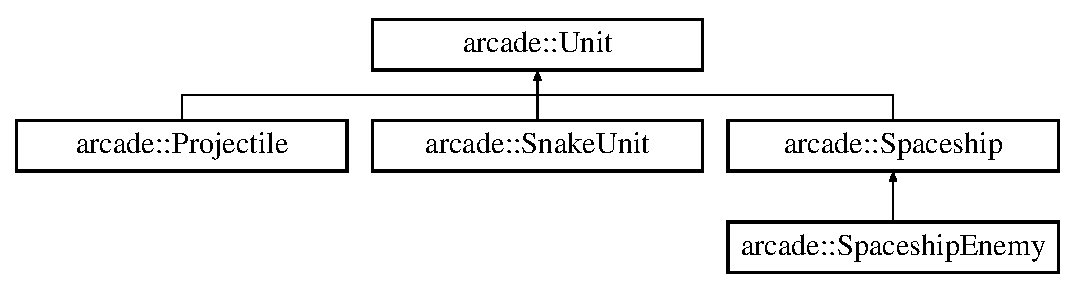
\includegraphics[height=3.000000cm]{classarcade_1_1_unit}
\end{center}
\end{figure}
\subsection*{Public Types}
\begin{DoxyCompactItemize}
\item 
enum \hyperlink{classarcade_1_1_unit_af418afeaba1f7fd5934b6ae1343215dd}{Direction} \{ \newline
\hyperlink{classarcade_1_1_unit_af418afeaba1f7fd5934b6ae1343215dda01d1f45d2a1f46111e0a7a4bb9bd5555}{UP} = 2, 
\hyperlink{classarcade_1_1_unit_af418afeaba1f7fd5934b6ae1343215dda5f32d341b3496680d6f76b2e27a5038b}{D\+O\+WN} = 3, 
\hyperlink{classarcade_1_1_unit_af418afeaba1f7fd5934b6ae1343215ddafb9de8c64a904e3e78e9a62907de7f6f}{L\+E\+FT} = 4, 
\hyperlink{classarcade_1_1_unit_af418afeaba1f7fd5934b6ae1343215ddab94e0ec58f3e9b07b9f65e3001e64171}{R\+I\+G\+HT} = 5, 
\newline
\hyperlink{classarcade_1_1_unit_af418afeaba1f7fd5934b6ae1343215dda5a33eaa50fc5e4fda0befda90cf68c60}{F\+O\+R\+W\+A\+RD} = 6
 \}
\end{DoxyCompactItemize}
\subsection*{Public Member Functions}
\begin{DoxyCompactItemize}
\item 
virtual \hyperlink{classarcade_1_1_unit_a44236fd92c37b80c2fda5356d8b6ec81}{$\sim$\+Unit} ()
\item 
\hyperlink{classarcade_1_1_unit_a34cb0964152e5039495031ec7be15613}{Unit} (const std\+::pair$<$ size\+\_\+t, size\+\_\+t $>$ \&\hyperlink{classarcade_1_1_unit_ab56f7df422277f97e7738cb4807fd62d}{position})
\item 
\hyperlink{classarcade_1_1_unit_abf639f95e434f9920cb6a342784e8d4e}{Unit} (size\+\_\+t \hyperlink{include_2_protocol_8hpp_a4dde988b1b2adba65ae3efa69f65d960}{x}, size\+\_\+t \hyperlink{include_2_protocol_8hpp_ab0580f504a7428539be299fa71565f30}{y})
\item 
virtual bool \hyperlink{classarcade_1_1_unit_a2a6a6feacea0fce220062be1115207b1}{move} (\hyperlink{classarcade_1_1_map}{Map} const \&map, \hyperlink{classarcade_1_1_unit_af418afeaba1f7fd5934b6ae1343215dd}{Direction} direction)
\item 
bool \hyperlink{classarcade_1_1_unit_a4a108f0a801a245f048366f787dcbe15}{move} (const \hyperlink{classarcade_1_1_map}{Map} \&map, \hyperlink{classarcade_1_1_unit_af418afeaba1f7fd5934b6ae1343215dd}{Direction} direction, size\+\_\+t offset\+Map\+Border)
\item 
virtual void \hyperlink{classarcade_1_1_unit_a59e206c30ea40c75f0a4e7165e510717}{move\+Up} ()
\item 
virtual void \hyperlink{classarcade_1_1_unit_a2c308fe563d0851f2a275694c9b0dc6c}{move\+Down} ()
\item 
virtual void \hyperlink{classarcade_1_1_unit_a17f28a5a98e7c24e8c1ea13897220d89}{move\+Left} ()
\item 
virtual void \hyperlink{classarcade_1_1_unit_a58ef633f19e9fe137006e8cdd3fb7d29}{move\+Right} ()
\item 
const std\+::pair$<$ size\+\_\+t, size\+\_\+t $>$ \& \hyperlink{classarcade_1_1_unit_a6ab43e77e961dc4192687ea730dd7712}{get\+Position} () const
\item 
void \hyperlink{classarcade_1_1_unit_ab53d6d5f92e49bfe5f500307e299599d}{set\+Position} (const std\+::pair$<$ size\+\_\+t, size\+\_\+t $>$ \&\hyperlink{classarcade_1_1_unit_ab56f7df422277f97e7738cb4807fd62d}{position})
\item 
void \hyperlink{classarcade_1_1_unit_a5b6beb5c96e174caf0ba0f0d14ccde8b}{set\+Position} (size\+\_\+t \hyperlink{include_2_protocol_8hpp_a4dde988b1b2adba65ae3efa69f65d960}{x}, size\+\_\+t \hyperlink{include_2_protocol_8hpp_ab0580f504a7428539be299fa71565f30}{y})
\item 
\hyperlink{classarcade_1_1_unit_af418afeaba1f7fd5934b6ae1343215dd}{Direction} \hyperlink{classarcade_1_1_unit_aa1a289e46e53c2c9bf7d80ef5571d08f}{get\+Opposite\+Direction} (\hyperlink{classarcade_1_1_unit_af418afeaba1f7fd5934b6ae1343215dd}{Direction} direction)
\item 
std\+::pair$<$ int, int $>$ \hyperlink{classarcade_1_1_unit_ada89038fcb7152ea19e2639e1bbc58ea}{convert\+Direction} (\hyperlink{classarcade_1_1_unit_af418afeaba1f7fd5934b6ae1343215dd}{Direction} direction)
\item 
bool \hyperlink{classarcade_1_1_unit_ab79c51d02d31cc6578cc25b202e4292d}{cmp\+Pos} (\hyperlink{classarcade_1_1_unit}{Unit} const \&unit)
\end{DoxyCompactItemize}
\subsection*{Protected Attributes}
\begin{DoxyCompactItemize}
\item 
std\+::pair$<$ size\+\_\+t, size\+\_\+t $>$ \hyperlink{classarcade_1_1_unit_ac9e7559836ec4e3b3bdcde00d3e3bb97}{initial\+Pos}
\item 
std\+::pair$<$ size\+\_\+t, size\+\_\+t $>$ \hyperlink{classarcade_1_1_unit_ab56f7df422277f97e7738cb4807fd62d}{position}
\end{DoxyCompactItemize}


\subsection{Member Enumeration Documentation}
\mbox{\Hypertarget{classarcade_1_1_unit_af418afeaba1f7fd5934b6ae1343215dd}\label{classarcade_1_1_unit_af418afeaba1f7fd5934b6ae1343215dd}} 
\index{arcade\+::\+Unit@{arcade\+::\+Unit}!Direction@{Direction}}
\index{Direction@{Direction}!arcade\+::\+Unit@{arcade\+::\+Unit}}
\subsubsection{\texorpdfstring{Direction}{Direction}}
{\footnotesize\ttfamily enum \hyperlink{classarcade_1_1_unit_af418afeaba1f7fd5934b6ae1343215dd}{arcade\+::\+Unit\+::\+Direction}}

\begin{DoxyEnumFields}{Enumerator}
\raisebox{\heightof{T}}[0pt][0pt]{\index{UP@{UP}!arcade\+::\+Unit@{arcade\+::\+Unit}}\index{arcade\+::\+Unit@{arcade\+::\+Unit}!UP@{UP}}}\mbox{\Hypertarget{classarcade_1_1_unit_af418afeaba1f7fd5934b6ae1343215dda01d1f45d2a1f46111e0a7a4bb9bd5555}\label{classarcade_1_1_unit_af418afeaba1f7fd5934b6ae1343215dda01d1f45d2a1f46111e0a7a4bb9bd5555}} 
UP&\\
\hline

\raisebox{\heightof{T}}[0pt][0pt]{\index{D\+O\+WN@{D\+O\+WN}!arcade\+::\+Unit@{arcade\+::\+Unit}}\index{arcade\+::\+Unit@{arcade\+::\+Unit}!D\+O\+WN@{D\+O\+WN}}}\mbox{\Hypertarget{classarcade_1_1_unit_af418afeaba1f7fd5934b6ae1343215dda5f32d341b3496680d6f76b2e27a5038b}\label{classarcade_1_1_unit_af418afeaba1f7fd5934b6ae1343215dda5f32d341b3496680d6f76b2e27a5038b}} 
D\+O\+WN&\\
\hline

\raisebox{\heightof{T}}[0pt][0pt]{\index{L\+E\+FT@{L\+E\+FT}!arcade\+::\+Unit@{arcade\+::\+Unit}}\index{arcade\+::\+Unit@{arcade\+::\+Unit}!L\+E\+FT@{L\+E\+FT}}}\mbox{\Hypertarget{classarcade_1_1_unit_af418afeaba1f7fd5934b6ae1343215ddafb9de8c64a904e3e78e9a62907de7f6f}\label{classarcade_1_1_unit_af418afeaba1f7fd5934b6ae1343215ddafb9de8c64a904e3e78e9a62907de7f6f}} 
L\+E\+FT&\\
\hline

\raisebox{\heightof{T}}[0pt][0pt]{\index{R\+I\+G\+HT@{R\+I\+G\+HT}!arcade\+::\+Unit@{arcade\+::\+Unit}}\index{arcade\+::\+Unit@{arcade\+::\+Unit}!R\+I\+G\+HT@{R\+I\+G\+HT}}}\mbox{\Hypertarget{classarcade_1_1_unit_af418afeaba1f7fd5934b6ae1343215ddab94e0ec58f3e9b07b9f65e3001e64171}\label{classarcade_1_1_unit_af418afeaba1f7fd5934b6ae1343215ddab94e0ec58f3e9b07b9f65e3001e64171}} 
R\+I\+G\+HT&\\
\hline

\raisebox{\heightof{T}}[0pt][0pt]{\index{F\+O\+R\+W\+A\+RD@{F\+O\+R\+W\+A\+RD}!arcade\+::\+Unit@{arcade\+::\+Unit}}\index{arcade\+::\+Unit@{arcade\+::\+Unit}!F\+O\+R\+W\+A\+RD@{F\+O\+R\+W\+A\+RD}}}\mbox{\Hypertarget{classarcade_1_1_unit_af418afeaba1f7fd5934b6ae1343215dda5a33eaa50fc5e4fda0befda90cf68c60}\label{classarcade_1_1_unit_af418afeaba1f7fd5934b6ae1343215dda5a33eaa50fc5e4fda0befda90cf68c60}} 
F\+O\+R\+W\+A\+RD&\\
\hline

\end{DoxyEnumFields}


\subsection{Constructor \& Destructor Documentation}
\mbox{\Hypertarget{classarcade_1_1_unit_a44236fd92c37b80c2fda5356d8b6ec81}\label{classarcade_1_1_unit_a44236fd92c37b80c2fda5356d8b6ec81}} 
\index{arcade\+::\+Unit@{arcade\+::\+Unit}!````~Unit@{$\sim$\+Unit}}
\index{````~Unit@{$\sim$\+Unit}!arcade\+::\+Unit@{arcade\+::\+Unit}}
\subsubsection{\texorpdfstring{$\sim$\+Unit()}{~Unit()}}
{\footnotesize\ttfamily arcade\+::\+Unit\+::$\sim$\+Unit (\begin{DoxyParamCaption}{ }\end{DoxyParamCaption})\hspace{0.3cm}{\ttfamily [virtual]}}

\mbox{\Hypertarget{classarcade_1_1_unit_a34cb0964152e5039495031ec7be15613}\label{classarcade_1_1_unit_a34cb0964152e5039495031ec7be15613}} 
\index{arcade\+::\+Unit@{arcade\+::\+Unit}!Unit@{Unit}}
\index{Unit@{Unit}!arcade\+::\+Unit@{arcade\+::\+Unit}}
\subsubsection{\texorpdfstring{Unit()}{Unit()}\hspace{0.1cm}{\footnotesize\ttfamily [1/2]}}
{\footnotesize\ttfamily arcade\+::\+Unit\+::\+Unit (\begin{DoxyParamCaption}\item[{const std\+::pair$<$ size\+\_\+t, size\+\_\+t $>$ \&}]{position }\end{DoxyParamCaption})}

\mbox{\Hypertarget{classarcade_1_1_unit_abf639f95e434f9920cb6a342784e8d4e}\label{classarcade_1_1_unit_abf639f95e434f9920cb6a342784e8d4e}} 
\index{arcade\+::\+Unit@{arcade\+::\+Unit}!Unit@{Unit}}
\index{Unit@{Unit}!arcade\+::\+Unit@{arcade\+::\+Unit}}
\subsubsection{\texorpdfstring{Unit()}{Unit()}\hspace{0.1cm}{\footnotesize\ttfamily [2/2]}}
{\footnotesize\ttfamily arcade\+::\+Unit\+::\+Unit (\begin{DoxyParamCaption}\item[{size\+\_\+t}]{x,  }\item[{size\+\_\+t}]{y }\end{DoxyParamCaption})}



\subsection{Member Function Documentation}
\mbox{\Hypertarget{classarcade_1_1_unit_ab79c51d02d31cc6578cc25b202e4292d}\label{classarcade_1_1_unit_ab79c51d02d31cc6578cc25b202e4292d}} 
\index{arcade\+::\+Unit@{arcade\+::\+Unit}!cmp\+Pos@{cmp\+Pos}}
\index{cmp\+Pos@{cmp\+Pos}!arcade\+::\+Unit@{arcade\+::\+Unit}}
\subsubsection{\texorpdfstring{cmp\+Pos()}{cmpPos()}}
{\footnotesize\ttfamily bool arcade\+::\+Unit\+::cmp\+Pos (\begin{DoxyParamCaption}\item[{\hyperlink{classarcade_1_1_unit}{Unit} const \&}]{unit }\end{DoxyParamCaption})}

\mbox{\Hypertarget{classarcade_1_1_unit_ada89038fcb7152ea19e2639e1bbc58ea}\label{classarcade_1_1_unit_ada89038fcb7152ea19e2639e1bbc58ea}} 
\index{arcade\+::\+Unit@{arcade\+::\+Unit}!convert\+Direction@{convert\+Direction}}
\index{convert\+Direction@{convert\+Direction}!arcade\+::\+Unit@{arcade\+::\+Unit}}
\subsubsection{\texorpdfstring{convert\+Direction()}{convertDirection()}}
{\footnotesize\ttfamily std\+::pair$<$ int, int $>$ arcade\+::\+Unit\+::convert\+Direction (\begin{DoxyParamCaption}\item[{\hyperlink{classarcade_1_1_unit_af418afeaba1f7fd5934b6ae1343215dd}{Direction}}]{direction }\end{DoxyParamCaption})}

\mbox{\Hypertarget{classarcade_1_1_unit_aa1a289e46e53c2c9bf7d80ef5571d08f}\label{classarcade_1_1_unit_aa1a289e46e53c2c9bf7d80ef5571d08f}} 
\index{arcade\+::\+Unit@{arcade\+::\+Unit}!get\+Opposite\+Direction@{get\+Opposite\+Direction}}
\index{get\+Opposite\+Direction@{get\+Opposite\+Direction}!arcade\+::\+Unit@{arcade\+::\+Unit}}
\subsubsection{\texorpdfstring{get\+Opposite\+Direction()}{getOppositeDirection()}}
{\footnotesize\ttfamily \hyperlink{classarcade_1_1_unit_af418afeaba1f7fd5934b6ae1343215dd}{arcade\+::\+Unit\+::\+Direction} arcade\+::\+Unit\+::get\+Opposite\+Direction (\begin{DoxyParamCaption}\item[{\hyperlink{classarcade_1_1_unit_af418afeaba1f7fd5934b6ae1343215dd}{Direction}}]{direction }\end{DoxyParamCaption})}

\mbox{\Hypertarget{classarcade_1_1_unit_a6ab43e77e961dc4192687ea730dd7712}\label{classarcade_1_1_unit_a6ab43e77e961dc4192687ea730dd7712}} 
\index{arcade\+::\+Unit@{arcade\+::\+Unit}!get\+Position@{get\+Position}}
\index{get\+Position@{get\+Position}!arcade\+::\+Unit@{arcade\+::\+Unit}}
\subsubsection{\texorpdfstring{get\+Position()}{getPosition()}}
{\footnotesize\ttfamily const std\+::pair$<$ size\+\_\+t, size\+\_\+t $>$ \& arcade\+::\+Unit\+::get\+Position (\begin{DoxyParamCaption}{ }\end{DoxyParamCaption}) const}

\mbox{\Hypertarget{classarcade_1_1_unit_a2a6a6feacea0fce220062be1115207b1}\label{classarcade_1_1_unit_a2a6a6feacea0fce220062be1115207b1}} 
\index{arcade\+::\+Unit@{arcade\+::\+Unit}!move@{move}}
\index{move@{move}!arcade\+::\+Unit@{arcade\+::\+Unit}}
\subsubsection{\texorpdfstring{move()}{move()}\hspace{0.1cm}{\footnotesize\ttfamily [1/2]}}
{\footnotesize\ttfamily bool arcade\+::\+Unit\+::move (\begin{DoxyParamCaption}\item[{\hyperlink{classarcade_1_1_map}{Map} const \&}]{map,  }\item[{\hyperlink{classarcade_1_1_unit_af418afeaba1f7fd5934b6ae1343215dd}{Direction}}]{direction }\end{DoxyParamCaption})\hspace{0.3cm}{\ttfamily [virtual]}}



Reimplemented in \hyperlink{classarcade_1_1_snake_unit_ac291cd07b71f42589e29157fdcf52416}{arcade\+::\+Snake\+Unit}.

\mbox{\Hypertarget{classarcade_1_1_unit_a4a108f0a801a245f048366f787dcbe15}\label{classarcade_1_1_unit_a4a108f0a801a245f048366f787dcbe15}} 
\index{arcade\+::\+Unit@{arcade\+::\+Unit}!move@{move}}
\index{move@{move}!arcade\+::\+Unit@{arcade\+::\+Unit}}
\subsubsection{\texorpdfstring{move()}{move()}\hspace{0.1cm}{\footnotesize\ttfamily [2/2]}}
{\footnotesize\ttfamily bool arcade\+::\+Unit\+::move (\begin{DoxyParamCaption}\item[{const \hyperlink{classarcade_1_1_map}{Map} \&}]{map,  }\item[{\hyperlink{classarcade_1_1_unit_af418afeaba1f7fd5934b6ae1343215dd}{Direction}}]{direction,  }\item[{size\+\_\+t}]{offset\+Map\+Border }\end{DoxyParamCaption})}

\mbox{\Hypertarget{classarcade_1_1_unit_a2c308fe563d0851f2a275694c9b0dc6c}\label{classarcade_1_1_unit_a2c308fe563d0851f2a275694c9b0dc6c}} 
\index{arcade\+::\+Unit@{arcade\+::\+Unit}!move\+Down@{move\+Down}}
\index{move\+Down@{move\+Down}!arcade\+::\+Unit@{arcade\+::\+Unit}}
\subsubsection{\texorpdfstring{move\+Down()}{moveDown()}}
{\footnotesize\ttfamily void arcade\+::\+Unit\+::move\+Down (\begin{DoxyParamCaption}{ }\end{DoxyParamCaption})\hspace{0.3cm}{\ttfamily [virtual]}}

\mbox{\Hypertarget{classarcade_1_1_unit_a17f28a5a98e7c24e8c1ea13897220d89}\label{classarcade_1_1_unit_a17f28a5a98e7c24e8c1ea13897220d89}} 
\index{arcade\+::\+Unit@{arcade\+::\+Unit}!move\+Left@{move\+Left}}
\index{move\+Left@{move\+Left}!arcade\+::\+Unit@{arcade\+::\+Unit}}
\subsubsection{\texorpdfstring{move\+Left()}{moveLeft()}}
{\footnotesize\ttfamily void arcade\+::\+Unit\+::move\+Left (\begin{DoxyParamCaption}{ }\end{DoxyParamCaption})\hspace{0.3cm}{\ttfamily [virtual]}}

\mbox{\Hypertarget{classarcade_1_1_unit_a58ef633f19e9fe137006e8cdd3fb7d29}\label{classarcade_1_1_unit_a58ef633f19e9fe137006e8cdd3fb7d29}} 
\index{arcade\+::\+Unit@{arcade\+::\+Unit}!move\+Right@{move\+Right}}
\index{move\+Right@{move\+Right}!arcade\+::\+Unit@{arcade\+::\+Unit}}
\subsubsection{\texorpdfstring{move\+Right()}{moveRight()}}
{\footnotesize\ttfamily void arcade\+::\+Unit\+::move\+Right (\begin{DoxyParamCaption}{ }\end{DoxyParamCaption})\hspace{0.3cm}{\ttfamily [virtual]}}

\mbox{\Hypertarget{classarcade_1_1_unit_a59e206c30ea40c75f0a4e7165e510717}\label{classarcade_1_1_unit_a59e206c30ea40c75f0a4e7165e510717}} 
\index{arcade\+::\+Unit@{arcade\+::\+Unit}!move\+Up@{move\+Up}}
\index{move\+Up@{move\+Up}!arcade\+::\+Unit@{arcade\+::\+Unit}}
\subsubsection{\texorpdfstring{move\+Up()}{moveUp()}}
{\footnotesize\ttfamily void arcade\+::\+Unit\+::move\+Up (\begin{DoxyParamCaption}{ }\end{DoxyParamCaption})\hspace{0.3cm}{\ttfamily [virtual]}}

\mbox{\Hypertarget{classarcade_1_1_unit_ab53d6d5f92e49bfe5f500307e299599d}\label{classarcade_1_1_unit_ab53d6d5f92e49bfe5f500307e299599d}} 
\index{arcade\+::\+Unit@{arcade\+::\+Unit}!set\+Position@{set\+Position}}
\index{set\+Position@{set\+Position}!arcade\+::\+Unit@{arcade\+::\+Unit}}
\subsubsection{\texorpdfstring{set\+Position()}{setPosition()}\hspace{0.1cm}{\footnotesize\ttfamily [1/2]}}
{\footnotesize\ttfamily void arcade\+::\+Unit\+::set\+Position (\begin{DoxyParamCaption}\item[{const std\+::pair$<$ size\+\_\+t, size\+\_\+t $>$ \&}]{position }\end{DoxyParamCaption})}

\mbox{\Hypertarget{classarcade_1_1_unit_a5b6beb5c96e174caf0ba0f0d14ccde8b}\label{classarcade_1_1_unit_a5b6beb5c96e174caf0ba0f0d14ccde8b}} 
\index{arcade\+::\+Unit@{arcade\+::\+Unit}!set\+Position@{set\+Position}}
\index{set\+Position@{set\+Position}!arcade\+::\+Unit@{arcade\+::\+Unit}}
\subsubsection{\texorpdfstring{set\+Position()}{setPosition()}\hspace{0.1cm}{\footnotesize\ttfamily [2/2]}}
{\footnotesize\ttfamily void arcade\+::\+Unit\+::set\+Position (\begin{DoxyParamCaption}\item[{size\+\_\+t}]{x,  }\item[{size\+\_\+t}]{y }\end{DoxyParamCaption})}



\subsection{Member Data Documentation}
\mbox{\Hypertarget{classarcade_1_1_unit_ac9e7559836ec4e3b3bdcde00d3e3bb97}\label{classarcade_1_1_unit_ac9e7559836ec4e3b3bdcde00d3e3bb97}} 
\index{arcade\+::\+Unit@{arcade\+::\+Unit}!initial\+Pos@{initial\+Pos}}
\index{initial\+Pos@{initial\+Pos}!arcade\+::\+Unit@{arcade\+::\+Unit}}
\subsubsection{\texorpdfstring{initial\+Pos}{initialPos}}
{\footnotesize\ttfamily std\+::pair$<$size\+\_\+t, size\+\_\+t$>$ arcade\+::\+Unit\+::initial\+Pos\hspace{0.3cm}{\ttfamily [protected]}}

\mbox{\Hypertarget{classarcade_1_1_unit_ab56f7df422277f97e7738cb4807fd62d}\label{classarcade_1_1_unit_ab56f7df422277f97e7738cb4807fd62d}} 
\index{arcade\+::\+Unit@{arcade\+::\+Unit}!position@{position}}
\index{position@{position}!arcade\+::\+Unit@{arcade\+::\+Unit}}
\subsubsection{\texorpdfstring{position}{position}}
{\footnotesize\ttfamily std\+::pair$<$size\+\_\+t , size\+\_\+t$>$ arcade\+::\+Unit\+::position\hspace{0.3cm}{\ttfamily [protected]}}



The documentation for this class was generated from the following files\+:\begin{DoxyCompactItemize}
\item 
include/\hyperlink{_unit_8hpp}{Unit.\+hpp}\item 
srcs/\hyperlink{_unit_8cpp}{Unit.\+cpp}\end{DoxyCompactItemize}

\hypertarget{structarcade_1_1_where_am_i}{}\section{arcade\+:\+:Where\+AmI Struct Reference}
\label{structarcade_1_1_where_am_i}\index{arcade\+::\+Where\+AmI@{arcade\+::\+Where\+AmI}}


{\ttfamily \#include $<$Protocol.\+hpp$>$}

\subsection*{Public Attributes}
\begin{DoxyCompactItemize}
\item 
\hyperlink{namespacearcade_a23d58aed7310b22b59e2b8f8ff8a5ffd}{Command\+Type} \hyperlink{structarcade_1_1_where_am_i_a566284e4a60ce85a0e899da77d13984d}{type}
\item 
uint16\+\_\+t \hyperlink{structarcade_1_1_where_am_i_a06592a4f9ac45feacc13c3792424b493}{lenght}
\item 
\hyperlink{structarcade_1_1_position}{Position} \hyperlink{structarcade_1_1_where_am_i_a0a3d3fd39432c3e7c1ffd03d04f07771}{position} \mbox{[}0\mbox{]}
\end{DoxyCompactItemize}


\subsection{Member Data Documentation}
\mbox{\Hypertarget{structarcade_1_1_where_am_i_a06592a4f9ac45feacc13c3792424b493}\label{structarcade_1_1_where_am_i_a06592a4f9ac45feacc13c3792424b493}} 
\index{arcade\+::\+Where\+AmI@{arcade\+::\+Where\+AmI}!lenght@{lenght}}
\index{lenght@{lenght}!arcade\+::\+Where\+AmI@{arcade\+::\+Where\+AmI}}
\subsubsection{\texorpdfstring{lenght}{lenght}}
{\footnotesize\ttfamily uint16\+\_\+t arcade\+::\+Where\+Am\+I\+::lenght}

\mbox{\Hypertarget{structarcade_1_1_where_am_i_a0a3d3fd39432c3e7c1ffd03d04f07771}\label{structarcade_1_1_where_am_i_a0a3d3fd39432c3e7c1ffd03d04f07771}} 
\index{arcade\+::\+Where\+AmI@{arcade\+::\+Where\+AmI}!position@{position}}
\index{position@{position}!arcade\+::\+Where\+AmI@{arcade\+::\+Where\+AmI}}
\subsubsection{\texorpdfstring{position}{position}}
{\footnotesize\ttfamily \hyperlink{structarcade_1_1_position}{Position} arcade\+::\+Where\+Am\+I\+::position\mbox{[}0\mbox{]}}

\mbox{\Hypertarget{structarcade_1_1_where_am_i_a566284e4a60ce85a0e899da77d13984d}\label{structarcade_1_1_where_am_i_a566284e4a60ce85a0e899da77d13984d}} 
\index{arcade\+::\+Where\+AmI@{arcade\+::\+Where\+AmI}!type@{type}}
\index{type@{type}!arcade\+::\+Where\+AmI@{arcade\+::\+Where\+AmI}}
\subsubsection{\texorpdfstring{type}{type}}
{\footnotesize\ttfamily \hyperlink{namespacearcade_a23d58aed7310b22b59e2b8f8ff8a5ffd}{Command\+Type} arcade\+::\+Where\+Am\+I\+::type}



The documentation for this struct was generated from the following file\+:\begin{DoxyCompactItemize}
\item 
include/\hyperlink{include_2_protocol_8hpp}{Protocol.\+hpp}\end{DoxyCompactItemize}

\chapter{File Documentation}
\hypertarget{_color_8cpp}{}\section{arcade\+Interfaces/\+Color.cpp File Reference}
\label{_color_8cpp}\index{arcade\+Interfaces/\+Color.\+cpp@{arcade\+Interfaces/\+Color.\+cpp}}
{\ttfamily \#include \char`\"{}Color.\+hpp\char`\"{}}\newline
\subsection*{Namespaces}
\begin{DoxyCompactItemize}
\item 
 \hyperlink{namespacearcade}{arcade}
\end{DoxyCompactItemize}

\hypertarget{_color_8hpp}{}\section{arcade\+Interfaces/\+Color.hpp File Reference}
\label{_color_8hpp}\index{arcade\+Interfaces/\+Color.\+hpp@{arcade\+Interfaces/\+Color.\+hpp}}
{\ttfamily \#include $<$cstdint$>$}\newline
\subsection*{Classes}
\begin{DoxyCompactItemize}
\item 
union \hyperlink{unionarcade_1_1_color}{arcade\+::\+Color}
\begin{DoxyCompactList}\small\item\em Union to store R\+G\+Ba color. \end{DoxyCompactList}\end{DoxyCompactItemize}
\subsection*{Namespaces}
\begin{DoxyCompactItemize}
\item 
 \hyperlink{namespacearcade}{arcade}
\end{DoxyCompactItemize}
\subsection*{Macros}
\begin{DoxyCompactItemize}
\item 
\#define \hyperlink{_color_8hpp_a30f87dfd7349d5165f116b550c35c6ed}{I\+S\+\_\+\+L\+I\+T\+T\+L\+E\+\_\+\+E\+N\+D\+I\+AN}~(\+\_\+\+\_\+\+B\+Y\+T\+E\+\_\+\+O\+R\+D\+E\+R\+\_\+\+\_\+ == \+\_\+\+\_\+\+O\+R\+D\+E\+R\+\_\+\+L\+I\+T\+T\+L\+E\+\_\+\+E\+N\+D\+I\+A\+N\+\_\+\+\_\+)
\end{DoxyCompactItemize}


\subsection{Macro Definition Documentation}
\mbox{\Hypertarget{_color_8hpp_a30f87dfd7349d5165f116b550c35c6ed}\label{_color_8hpp_a30f87dfd7349d5165f116b550c35c6ed}} 
\index{Color.\+hpp@{Color.\+hpp}!I\+S\+\_\+\+L\+I\+T\+T\+L\+E\+\_\+\+E\+N\+D\+I\+AN@{I\+S\+\_\+\+L\+I\+T\+T\+L\+E\+\_\+\+E\+N\+D\+I\+AN}}
\index{I\+S\+\_\+\+L\+I\+T\+T\+L\+E\+\_\+\+E\+N\+D\+I\+AN@{I\+S\+\_\+\+L\+I\+T\+T\+L\+E\+\_\+\+E\+N\+D\+I\+AN}!Color.\+hpp@{Color.\+hpp}}
\subsubsection{\texorpdfstring{I\+S\+\_\+\+L\+I\+T\+T\+L\+E\+\_\+\+E\+N\+D\+I\+AN}{IS\_LITTLE\_ENDIAN}}
{\footnotesize\ttfamily \#define I\+S\+\_\+\+L\+I\+T\+T\+L\+E\+\_\+\+E\+N\+D\+I\+AN~(\+\_\+\+\_\+\+B\+Y\+T\+E\+\_\+\+O\+R\+D\+E\+R\+\_\+\+\_\+ == \+\_\+\+\_\+\+O\+R\+D\+E\+R\+\_\+\+L\+I\+T\+T\+L\+E\+\_\+\+E\+N\+D\+I\+A\+N\+\_\+\+\_\+)}


\hypertarget{_event_8hpp}{}\section{arcade\+Interfaces/\+Event.hpp File Reference}
\label{_event_8hpp}\index{arcade\+Interfaces/\+Event.\+hpp@{arcade\+Interfaces/\+Event.\+hpp}}
\subsection*{Classes}
\begin{DoxyCompactItemize}
\item 
struct \hyperlink{structarcade_1_1_mouse_pos}{arcade\+::\+Mouse\+Pos}
\begin{DoxyCompactList}\small\item\em Mouse position (on the scale map) \end{DoxyCompactList}\item 
struct \hyperlink{structarcade_1_1_event}{arcade\+::\+Event}
\begin{DoxyCompactList}\small\item\em Description of an event. \end{DoxyCompactList}\end{DoxyCompactItemize}
\subsection*{Namespaces}
\begin{DoxyCompactItemize}
\item 
 \hyperlink{namespacearcade}{arcade}
\end{DoxyCompactItemize}
\subsection*{Enumerations}
\begin{DoxyCompactItemize}
\item 
enum \hyperlink{namespacearcade_a608583b2070905ecc26e957409bb4f93}{arcade\+::\+Event\+Type} \{ \newline
\hyperlink{namespacearcade_a608583b2070905ecc26e957409bb4f93a1145fba0ebe09714077bf1f354414a35}{arcade\+::\+E\+T\+\_\+\+N\+O\+NE} = -\/1, 
\hyperlink{namespacearcade_a608583b2070905ecc26e957409bb4f93a47b5732315dd08e58ac45c37b376959a}{arcade\+::\+E\+T\+\_\+\+K\+E\+Y\+B\+O\+A\+RD}, 
\hyperlink{namespacearcade_a608583b2070905ecc26e957409bb4f93a2e94482647f6c5cf2ff95e092799c180}{arcade\+::\+E\+T\+\_\+\+M\+O\+U\+SE}, 
\hyperlink{namespacearcade_a608583b2070905ecc26e957409bb4f93ad137ec8c2a95fffda902f81bd0d98a31}{arcade\+::\+E\+T\+\_\+\+B\+U\+T\+T\+ON}, 
\newline
\hyperlink{namespacearcade_a608583b2070905ecc26e957409bb4f93a1518d56271dbaa90f6ba57a710473f14}{arcade\+::\+E\+T\+\_\+\+J\+O\+Y\+S\+T\+I\+CK}, 
\hyperlink{namespacearcade_a608583b2070905ecc26e957409bb4f93a34fbadb208ad07f25a8f30c8465a84bb}{arcade\+::\+E\+T\+\_\+\+Q\+U\+IT}, 
\hyperlink{namespacearcade_a608583b2070905ecc26e957409bb4f93ae818f5c6d611ac4ca126b0b7fd328b15}{arcade\+::\+N\+B\+\_\+\+E\+V\+E\+N\+T\+\_\+\+T\+Y\+PE}
 \}\begin{DoxyCompactList}\small\item\em General event type. \end{DoxyCompactList}
\item 
enum \hyperlink{namespacearcade_a1b6c05b243c7e94d71fb328705e619bd}{arcade\+::\+Action\+Type} \{ \newline
\hyperlink{namespacearcade_a1b6c05b243c7e94d71fb328705e619bdaac3c7c13e932f57d116c97d454019c5d}{arcade\+::\+A\+T\+\_\+\+N\+O\+NE} = -\/1, 
\hyperlink{namespacearcade_a1b6c05b243c7e94d71fb328705e619bda64dc691d8dfa7dc0571d226b42dfea6e}{arcade\+::\+A\+T\+\_\+\+P\+R\+E\+S\+S\+ED}, 
\hyperlink{namespacearcade_a1b6c05b243c7e94d71fb328705e619bda8e0c4a910dc5fc07e5231bad0052ddec}{arcade\+::\+A\+T\+\_\+\+R\+E\+L\+E\+A\+S\+ED}, 
\hyperlink{namespacearcade_a1b6c05b243c7e94d71fb328705e619bdaa2d5c4829c8962e701fbe019c829a3df}{arcade\+::\+A\+T\+\_\+\+M\+O\+V\+ED}, 
\newline
\hyperlink{namespacearcade_a1b6c05b243c7e94d71fb328705e619bda757f0462f88c882a093d7b66cf48bb90}{arcade\+::\+A\+T\+\_\+\+C\+O\+N\+N\+E\+C\+T\+ED}, 
\hyperlink{namespacearcade_a1b6c05b243c7e94d71fb328705e619bda0cd465f408a5f63b67856d4f71fe4fe5}{arcade\+::\+A\+T\+\_\+\+D\+I\+S\+C\+O\+N\+N\+E\+C\+T\+ED}, 
\hyperlink{namespacearcade_a1b6c05b243c7e94d71fb328705e619bdac98b0e1cf89751f47ff6dda67f210c4e}{arcade\+::\+N\+B\+\_\+\+A\+C\+T\+I\+O\+N\+\_\+\+T\+Y\+PE}
 \}\begin{DoxyCompactList}\small\item\em General action type. \end{DoxyCompactList}
\item 
enum \hyperlink{namespacearcade_a347918e3b31df21087660f19962ff80e}{arcade\+::\+Keyboard\+Key} \{ \newline
\hyperlink{namespacearcade_a347918e3b31df21087660f19962ff80ea7e50ad14d5bdcaacd8efec4a0dd76cb4}{arcade\+::\+K\+B\+\_\+\+N\+O\+NE} = -\/1, 
\hyperlink{namespacearcade_a347918e3b31df21087660f19962ff80ea505f15ad3d5f7c3165ded3446e95adca}{arcade\+::\+K\+B\+\_\+A}, 
\hyperlink{namespacearcade_a347918e3b31df21087660f19962ff80ea4764dccda37fb50788b91d20685f050e}{arcade\+::\+K\+B\+\_\+B}, 
\hyperlink{namespacearcade_a347918e3b31df21087660f19962ff80eab34b9cc5aba82a8e276569fea108a868}{arcade\+::\+K\+B\+\_\+C}, 
\newline
\hyperlink{namespacearcade_a347918e3b31df21087660f19962ff80ea182eea2e706a783af701322b1f0cc306}{arcade\+::\+K\+B\+\_\+D}, 
\hyperlink{namespacearcade_a347918e3b31df21087660f19962ff80eaa898e8ea3ae807a5a27ec94461227e35}{arcade\+::\+K\+B\+\_\+E}, 
\hyperlink{namespacearcade_a347918e3b31df21087660f19962ff80eac3703f943026cc3ab8e5bbc23ab17c55}{arcade\+::\+K\+B\+\_\+F}, 
\hyperlink{namespacearcade_a347918e3b31df21087660f19962ff80eaa95e02508e28fb8a0a36b62313fef0c4}{arcade\+::\+K\+B\+\_\+G}, 
\newline
\hyperlink{namespacearcade_a347918e3b31df21087660f19962ff80ea1b4e1c015905a2a3bbf4f0d58f11a3cf}{arcade\+::\+K\+B\+\_\+H}, 
\hyperlink{namespacearcade_a347918e3b31df21087660f19962ff80ea12cdc4e55071f238c01bdc0bbcfc9a83}{arcade\+::\+K\+B\+\_\+I}, 
\hyperlink{namespacearcade_a347918e3b31df21087660f19962ff80eae91b8c12be1a2cab1ff6782395fe6032}{arcade\+::\+K\+B\+\_\+J}, 
\hyperlink{namespacearcade_a347918e3b31df21087660f19962ff80ea37b75418f8e8fa87d5c9c25925d8000b}{arcade\+::\+K\+B\+\_\+K}, 
\newline
\hyperlink{namespacearcade_a347918e3b31df21087660f19962ff80ea8552339890c72f5dc81339f3ac545976}{arcade\+::\+K\+B\+\_\+L}, 
\hyperlink{namespacearcade_a347918e3b31df21087660f19962ff80ead8ea4df324a0977d9f0c22eb265e1376}{arcade\+::\+K\+B\+\_\+M}, 
\hyperlink{namespacearcade_a347918e3b31df21087660f19962ff80eaaaecb69237e2f8df568ab83b673a3d3b}{arcade\+::\+K\+B\+\_\+N}, 
\hyperlink{namespacearcade_a347918e3b31df21087660f19962ff80ea2ae9c121c20d02db9861b5362da2f526}{arcade\+::\+K\+B\+\_\+O}, 
\newline
\hyperlink{namespacearcade_a347918e3b31df21087660f19962ff80ea1d9f81f6e9b4850f3d51074319f40167}{arcade\+::\+K\+B\+\_\+P}, 
\hyperlink{namespacearcade_a347918e3b31df21087660f19962ff80ea3a264e82a71bd547a4608ccbe63d572c}{arcade\+::\+K\+B\+\_\+Q}, 
\hyperlink{namespacearcade_a347918e3b31df21087660f19962ff80eac105ce9cc677445b8ae4a50f2fd31b91}{arcade\+::\+K\+B\+\_\+R}, 
\hyperlink{namespacearcade_a347918e3b31df21087660f19962ff80ea934a27a34f63249459efaf87836d5209}{arcade\+::\+K\+B\+\_\+S}, 
\newline
\hyperlink{namespacearcade_a347918e3b31df21087660f19962ff80ea6927932508deb69e16d030e750587dc6}{arcade\+::\+K\+B\+\_\+T}, 
\hyperlink{namespacearcade_a347918e3b31df21087660f19962ff80eafba8e94b47c459533026a492e3ff818f}{arcade\+::\+K\+B\+\_\+U}, 
\hyperlink{namespacearcade_a347918e3b31df21087660f19962ff80eac231564808bf288004adbc3e57dcbd51}{arcade\+::\+K\+B\+\_\+V}, 
\hyperlink{namespacearcade_a347918e3b31df21087660f19962ff80eab5c1bbef9cc3116be7842f29f714e333}{arcade\+::\+K\+B\+\_\+W}, 
\newline
\hyperlink{namespacearcade_a347918e3b31df21087660f19962ff80ea30ef88e6cca8cd52d229af52144667e4}{arcade\+::\+K\+B\+\_\+X}, 
\hyperlink{namespacearcade_a347918e3b31df21087660f19962ff80ea9ef652a6a08f4a589285e54290e6f3b9}{arcade\+::\+K\+B\+\_\+Y}, 
\hyperlink{namespacearcade_a347918e3b31df21087660f19962ff80ea6bcddfe2b157ccbc3dd81cc1f0d6b313}{arcade\+::\+K\+B\+\_\+Z}, 
\hyperlink{namespacearcade_a347918e3b31df21087660f19962ff80eabb2fa1524c90159128c864935087b2b0}{arcade\+::\+K\+B\+\_\+0}, 
\newline
\hyperlink{namespacearcade_a347918e3b31df21087660f19962ff80eab674af590fc2261a7b9b8f5bb8a13f58}{arcade\+::\+K\+B\+\_\+1}, 
\hyperlink{namespacearcade_a347918e3b31df21087660f19962ff80ea66a791790c422d52e420d5a78e664f15}{arcade\+::\+K\+B\+\_\+2}, 
\hyperlink{namespacearcade_a347918e3b31df21087660f19962ff80eacace6038d1284f630f2808e39ff048fb}{arcade\+::\+K\+B\+\_\+3}, 
\hyperlink{namespacearcade_a347918e3b31df21087660f19962ff80ea5867e6c5ec0d784a10d164458efc13bb}{arcade\+::\+K\+B\+\_\+4}, 
\newline
\hyperlink{namespacearcade_a347918e3b31df21087660f19962ff80eaf1a2ef7803e123c1f6ee5f37b504d516}{arcade\+::\+K\+B\+\_\+5}, 
\hyperlink{namespacearcade_a347918e3b31df21087660f19962ff80ea0ee857f52a615bc4082a939d2d123d0a}{arcade\+::\+K\+B\+\_\+6}, 
\hyperlink{namespacearcade_a347918e3b31df21087660f19962ff80ea83200f9f3759451a8e93923f3c3558fb}{arcade\+::\+K\+B\+\_\+7}, 
\hyperlink{namespacearcade_a347918e3b31df21087660f19962ff80ea6a9bc51970df8bad5bcc52a160bf832f}{arcade\+::\+K\+B\+\_\+8}, 
\newline
\hyperlink{namespacearcade_a347918e3b31df21087660f19962ff80ea22e0ef6bf481c5775bc08319ed1a29cb}{arcade\+::\+K\+B\+\_\+9}, 
\hyperlink{namespacearcade_a347918e3b31df21087660f19962ff80eab451e10c664e4910b93db2495ff3b89c}{arcade\+::\+K\+B\+\_\+\+A\+R\+R\+O\+W\+\_\+\+L\+E\+FT}, 
\hyperlink{namespacearcade_a347918e3b31df21087660f19962ff80ea03d7fc107a30c35437d31965a1c0c217}{arcade\+::\+K\+B\+\_\+\+A\+R\+R\+O\+W\+\_\+\+R\+I\+G\+HT}, 
\hyperlink{namespacearcade_a347918e3b31df21087660f19962ff80ea1417060d82a532b2ddd28a903071ca11}{arcade\+::\+K\+B\+\_\+\+A\+R\+R\+O\+W\+\_\+\+UP}, 
\newline
\hyperlink{namespacearcade_a347918e3b31df21087660f19962ff80ea45584980d376ad7b6e3b3825fb80a4d6}{arcade\+::\+K\+B\+\_\+\+A\+R\+R\+O\+W\+\_\+\+D\+O\+WN}, 
\hyperlink{namespacearcade_a347918e3b31df21087660f19962ff80ea5ddc9b7df97f07fd252cf19389258dd8}{arcade\+::\+K\+B\+\_\+\+S\+P\+A\+CE}, 
\hyperlink{namespacearcade_a347918e3b31df21087660f19962ff80ea2580ddb2709167f0023b40d9c0deb378}{arcade\+::\+K\+B\+\_\+\+E\+N\+T\+ER}, 
\hyperlink{namespacearcade_a347918e3b31df21087660f19962ff80ea15794d5c1ac0898c0c2e4e98d37e3857}{arcade\+::\+K\+B\+\_\+\+B\+A\+C\+K\+S\+P\+A\+CE}, 
\newline
\hyperlink{namespacearcade_a347918e3b31df21087660f19962ff80ea2d6a8932ee3191b0aa9a146afec40c46}{arcade\+::\+K\+B\+\_\+\+L\+C\+T\+RL}, 
\hyperlink{namespacearcade_a347918e3b31df21087660f19962ff80ea5de5b3b0fe89850f39a10dd3bca918cb}{arcade\+::\+K\+B\+\_\+\+R\+C\+T\+RL}, 
\hyperlink{namespacearcade_a347918e3b31df21087660f19962ff80eafdc71fbb454596e9518726ea821c24d1}{arcade\+::\+K\+B\+\_\+\+L\+A\+LT}, 
\hyperlink{namespacearcade_a347918e3b31df21087660f19962ff80ea72b77d9cc20b5735e14670aef9274645}{arcade\+::\+K\+B\+\_\+\+R\+A\+LT}, 
\newline
\hyperlink{namespacearcade_a347918e3b31df21087660f19962ff80ea0eb88f38a01e761e7261c473a5ba11f8}{arcade\+::\+K\+B\+\_\+\+L\+S\+H\+I\+FT}, 
\hyperlink{namespacearcade_a347918e3b31df21087660f19962ff80ea396d5e142ef21bc3cda13431e9fa24c0}{arcade\+::\+K\+B\+\_\+\+R\+S\+H\+I\+FT}, 
\hyperlink{namespacearcade_a347918e3b31df21087660f19962ff80ea8742e736d70c460576c4cebe40ffb89f}{arcade\+::\+K\+B\+\_\+\+C\+A\+P\+S\+L\+O\+CK}, 
\hyperlink{namespacearcade_a347918e3b31df21087660f19962ff80eae9879e6a709ead9a4a9f35e148b486b1}{arcade\+::\+K\+B\+\_\+\+T\+AB}, 
\newline
\hyperlink{namespacearcade_a347918e3b31df21087660f19962ff80eab99011f38f2af81c272dc654c5ea406a}{arcade\+::\+K\+B\+\_\+\+E\+S\+C\+A\+PE}, 
\hyperlink{namespacearcade_a347918e3b31df21087660f19962ff80ea673b42fd73696cf21fa529161241f991}{arcade\+::\+K\+B\+\_\+\+P\+A\+G\+E\+UP}, 
\hyperlink{namespacearcade_a347918e3b31df21087660f19962ff80ea6b65b30768ade9382504190406fc4dc3}{arcade\+::\+K\+B\+\_\+\+P\+A\+G\+E\+D\+O\+WN}, 
\hyperlink{namespacearcade_a347918e3b31df21087660f19962ff80ea04a05eb2f1301c3baffe8c7137fb06dc}{arcade\+::\+K\+B\+\_\+\+H\+O\+ME}, 
\newline
\hyperlink{namespacearcade_a347918e3b31df21087660f19962ff80ea7a15e19dadaff3e156bbd72a00738fe8}{arcade\+::\+K\+B\+\_\+\+E\+ND}, 
\hyperlink{namespacearcade_a347918e3b31df21087660f19962ff80ea75d48628972e9758781eda5e6d4e2eb4}{arcade\+::\+K\+B\+\_\+\+F\+N1}, 
\hyperlink{namespacearcade_a347918e3b31df21087660f19962ff80ea0a85073270d11b51f542be97e43b4d19}{arcade\+::\+K\+B\+\_\+\+F\+N2}, 
\hyperlink{namespacearcade_a347918e3b31df21087660f19962ff80ea0b95bd1641d79c3186dfdd7c0e30b8e0}{arcade\+::\+K\+B\+\_\+\+F\+N3}, 
\newline
\hyperlink{namespacearcade_a347918e3b31df21087660f19962ff80ea43b7323fda1dc41c9ab0847cda9e734a}{arcade\+::\+K\+B\+\_\+\+F\+N4}, 
\hyperlink{namespacearcade_a347918e3b31df21087660f19962ff80ea823211a5d68e66b4f626a232e0f93877}{arcade\+::\+K\+B\+\_\+\+F\+N5}, 
\hyperlink{namespacearcade_a347918e3b31df21087660f19962ff80ea16ddf267a9d6b464562c3e3d4ade8bee}{arcade\+::\+K\+B\+\_\+\+F\+N6}, 
\hyperlink{namespacearcade_a347918e3b31df21087660f19962ff80eab2f3f370ae5a0c69acf0ef039d2af3a1}{arcade\+::\+K\+B\+\_\+\+F\+N7}, 
\newline
\hyperlink{namespacearcade_a347918e3b31df21087660f19962ff80eac53e73cb2648c9a3c1a7064a699b16ef}{arcade\+::\+K\+B\+\_\+\+F\+N8}, 
\hyperlink{namespacearcade_a347918e3b31df21087660f19962ff80eaa11b588576bf36d8d4196eaa53ce0ba2}{arcade\+::\+K\+B\+\_\+\+F\+N9}, 
\hyperlink{namespacearcade_a347918e3b31df21087660f19962ff80ea42e633880b1f7f2aa680af765a493129}{arcade\+::\+K\+B\+\_\+\+F\+N10}, 
\hyperlink{namespacearcade_a347918e3b31df21087660f19962ff80ea2d97bbb2def613489d124763db3122e8}{arcade\+::\+K\+B\+\_\+\+F\+N11}, 
\newline
\hyperlink{namespacearcade_a347918e3b31df21087660f19962ff80ea9111ee038a53429265950d9b804a6924}{arcade\+::\+K\+B\+\_\+\+F\+N12}, 
\hyperlink{namespacearcade_a347918e3b31df21087660f19962ff80eac14f14d5974343df42c51ff9077e4608}{arcade\+::\+K\+B\+\_\+\+C\+O\+M\+MA}, 
\hyperlink{namespacearcade_a347918e3b31df21087660f19962ff80ea76d6ae297e7e894b9fe9f207f3554887}{arcade\+::\+K\+B\+\_\+\+D\+OT}, 
\hyperlink{namespacearcade_a347918e3b31df21087660f19962ff80ea158a96f344bce722acdbec3cc929468b}{arcade\+::\+K\+B\+\_\+\+S\+L\+A\+SH}, 
\newline
\hyperlink{namespacearcade_a347918e3b31df21087660f19962ff80eacf2cd3609a488585897a14256730a33a}{arcade\+::\+K\+B\+\_\+\+I\+N\+F\+E\+R\+I\+OR}, 
\hyperlink{namespacearcade_a347918e3b31df21087660f19962ff80ea15767e6cbaf8b78d1eb42b355f816c61}{arcade\+::\+K\+B\+\_\+\+S\+U\+P\+E\+R\+I\+OR}, 
\hyperlink{namespacearcade_a347918e3b31df21087660f19962ff80ea60dccaebd08351992b1e92e65a4e3533}{arcade\+::\+K\+B\+\_\+\+Q\+U\+E\+S\+T\+I\+ON}, 
\hyperlink{namespacearcade_a347918e3b31df21087660f19962ff80ea939a88f10493ec89f8d41c9397dc44b7}{arcade\+::\+K\+B\+\_\+\+S\+E\+M\+I\+C\+O\+L\+ON}, 
\newline
\hyperlink{namespacearcade_a347918e3b31df21087660f19962ff80ea0adde44293346394a688436a67e04633}{arcade\+::\+K\+B\+\_\+\+C\+O\+L\+ON}, 
\hyperlink{namespacearcade_a347918e3b31df21087660f19962ff80ea76a6219eef24df6f69c9c49bc43560ee}{arcade\+::\+K\+B\+\_\+\+S\+I\+M\+P\+L\+E\+Q\+U\+O\+TE}, 
\hyperlink{namespacearcade_a347918e3b31df21087660f19962ff80ea3f773bb8bcbcd73292dcfaad3b0b90ea}{arcade\+::\+K\+B\+\_\+\+D\+O\+U\+B\+L\+E\+Q\+U\+O\+TE}, 
\hyperlink{namespacearcade_a347918e3b31df21087660f19962ff80eae2f3c46d71cd0f0dacdd598f09cb1718}{arcade\+::\+K\+B\+\_\+\+L\+E\+F\+T\+B\+R\+A\+CE}, 
\newline
\hyperlink{namespacearcade_a347918e3b31df21087660f19962ff80ea6b9a875877d5fe5ab50b2ffa38db20be}{arcade\+::\+K\+B\+\_\+\+R\+I\+G\+H\+T\+B\+R\+A\+CE}, 
\hyperlink{namespacearcade_a347918e3b31df21087660f19962ff80ea8bcd0be6537486775e9025148903d346}{arcade\+::\+K\+B\+\_\+\+L\+E\+F\+T\+B\+R\+A\+C\+K\+ET}, 
\hyperlink{namespacearcade_a347918e3b31df21087660f19962ff80ea9c75b4de4cb3ef786d3b4ab3a5a07511}{arcade\+::\+K\+B\+\_\+\+R\+I\+G\+H\+T\+B\+R\+A\+C\+K\+ET}, 
\hyperlink{namespacearcade_a347918e3b31df21087660f19962ff80eaf0a906f50d130a3335a63ac480994710}{arcade\+::\+K\+B\+\_\+\+L\+E\+F\+T\+P\+A\+R\+EN}, 
\newline
\hyperlink{namespacearcade_a347918e3b31df21087660f19962ff80ea9dcd2a623be9411235b7879458810cf9}{arcade\+::\+K\+B\+\_\+\+R\+I\+G\+H\+T\+P\+A\+R\+EN}, 
\hyperlink{namespacearcade_a347918e3b31df21087660f19962ff80eacf11e7cc80ec696fa05c1b339a020995}{arcade\+::\+K\+B\+\_\+\+B\+A\+C\+K\+S\+L\+A\+SH}, 
\hyperlink{namespacearcade_a347918e3b31df21087660f19962ff80eafa053222bafb910d7a0e1f114e1ed0c9}{arcade\+::\+K\+B\+\_\+\+V\+E\+R\+T\+I\+C\+A\+L\+B\+AR}, 
\hyperlink{namespacearcade_a347918e3b31df21087660f19962ff80ea906b40548cc6113c9d8c2f7b5481b13c}{arcade\+::\+K\+B\+\_\+\+E\+X\+C\+L\+A\+M\+A\+T\+I\+ON}, 
\newline
\hyperlink{namespacearcade_a347918e3b31df21087660f19962ff80ea14cf7afb33d05e90ba7a0c053a4a7e81}{arcade\+::\+K\+B\+\_\+\+A\+T\+S\+Y\+M\+B\+OL}, 
\hyperlink{namespacearcade_a347918e3b31df21087660f19962ff80eab2661ab89070346d6d4e320bc7cfb799}{arcade\+::\+K\+B\+\_\+\+H\+A\+S\+H\+T\+AG}, 
\hyperlink{namespacearcade_a347918e3b31df21087660f19962ff80ea37a32fb5cb993a48b602d555e7bc9e2f}{arcade\+::\+K\+B\+\_\+\+D\+O\+L\+L\+AR}, 
\hyperlink{namespacearcade_a347918e3b31df21087660f19962ff80ea160c8c6e8d6b67c30e43c462d69b26df}{arcade\+::\+K\+B\+\_\+\+P\+E\+R\+C\+E\+NT}, 
\newline
\hyperlink{namespacearcade_a347918e3b31df21087660f19962ff80ea8f375b35b02eacd740c051ea943ef8e4}{arcade\+::\+K\+B\+\_\+\+C\+I\+R\+C\+U\+M\+F\+L\+EX}, 
\hyperlink{namespacearcade_a347918e3b31df21087660f19962ff80ea651f68ff2cc76d96130083261865a8f1}{arcade\+::\+K\+B\+\_\+\+A\+M\+P\+E\+R\+S\+A\+ND}, 
\hyperlink{namespacearcade_a347918e3b31df21087660f19962ff80eab2c2612f919800f0343a4f3fbf48e989}{arcade\+::\+K\+B\+\_\+\+A\+S\+T\+E\+R\+I\+SK}, 
\hyperlink{namespacearcade_a347918e3b31df21087660f19962ff80eaf17f8cf56aab21c19db22d9094179e99}{arcade\+::\+K\+B\+\_\+\+U\+N\+D\+E\+R\+S\+C\+O\+RE}, 
\newline
\hyperlink{namespacearcade_a347918e3b31df21087660f19962ff80eaaee640f7de93992be6a22d7950e2f59f}{arcade\+::\+K\+B\+\_\+\+M\+I\+N\+US}, 
\hyperlink{namespacearcade_a347918e3b31df21087660f19962ff80ea700ed87915dc8a99064ad33498ddc9a6}{arcade\+::\+K\+B\+\_\+\+P\+L\+US}, 
\hyperlink{namespacearcade_a347918e3b31df21087660f19962ff80ea7810fb4ea4fb7943c7dc9616305ac472}{arcade\+::\+K\+B\+\_\+\+E\+Q\+U\+A\+LS}, 
\hyperlink{namespacearcade_a347918e3b31df21087660f19962ff80ead477e3c7d899002dd64876ae6a0cff2a}{arcade\+::\+K\+B\+\_\+\+D\+E\+L\+E\+TE}, 
\newline
\hyperlink{namespacearcade_a347918e3b31df21087660f19962ff80eaa1c3de811b5803a1a65b6ae0e45cc0b1}{arcade\+::\+N\+B\+\_\+\+K\+E\+Y\+B\+O\+A\+R\+D\+\_\+\+K\+EY}
 \}\begin{DoxyCompactList}\small\item\em Common keyboard keys. \end{DoxyCompactList}
\item 
enum \hyperlink{namespacearcade_a41017b6e882fbcad335f303c7950e4bf}{arcade\+::\+Mouse\+Key} \{ \newline
\hyperlink{namespacearcade_a41017b6e882fbcad335f303c7950e4bfa91c72d27e507baddb57e88eed37e2f2f}{arcade\+::\+M\+\_\+\+N\+O\+NE} = -\/1, 
\hyperlink{namespacearcade_a41017b6e882fbcad335f303c7950e4bfac1daae4d5f7b313ca00cb5fe383f343a}{arcade\+::\+M\+\_\+\+L\+E\+F\+T\+\_\+\+C\+L\+I\+CK}, 
\hyperlink{namespacearcade_a41017b6e882fbcad335f303c7950e4bfa72602a4642a4aff4128b701b17623806}{arcade\+::\+M\+\_\+\+R\+I\+G\+H\+T\+\_\+\+C\+L\+I\+CK}, 
\hyperlink{namespacearcade_a41017b6e882fbcad335f303c7950e4bfabcc3fea48c87e2a1f4786260104c7106}{arcade\+::\+M\+\_\+\+M\+I\+D\+D\+L\+E\+\_\+\+C\+L\+I\+CK}, 
\newline
\hyperlink{namespacearcade_a41017b6e882fbcad335f303c7950e4bfa6d93c3604c3778ac9aeb9249193ce2e2}{arcade\+::\+M\+\_\+\+S\+C\+R\+O\+L\+L\+\_\+\+UP}, 
\hyperlink{namespacearcade_a41017b6e882fbcad335f303c7950e4bfa0ef545aca48798c75ea921a90bf763df}{arcade\+::\+M\+\_\+\+S\+C\+R\+O\+L\+L\+\_\+\+D\+O\+WN}, 
\hyperlink{namespacearcade_a41017b6e882fbcad335f303c7950e4bfa2f33f0f811dbc434a032019ba9fb9a59}{arcade\+::\+M\+\_\+\+B\+T0}, 
\hyperlink{namespacearcade_a41017b6e882fbcad335f303c7950e4bfa26c806f39133da7426933190c0c4e97b}{arcade\+::\+M\+\_\+\+B\+T1}, 
\newline
\hyperlink{namespacearcade_a41017b6e882fbcad335f303c7950e4bfaf8fee919e8dc5d7eac244526b9358c89}{arcade\+::\+M\+\_\+\+B\+T2}, 
\hyperlink{namespacearcade_a41017b6e882fbcad335f303c7950e4bfa75085062db55a2e0d77b290463e4f6e9}{arcade\+::\+M\+\_\+\+B\+T3}, 
\hyperlink{namespacearcade_a41017b6e882fbcad335f303c7950e4bfa1b98d7b9b0493ec5fb3f9fad1ed8e297}{arcade\+::\+M\+\_\+\+B\+T4}, 
\hyperlink{namespacearcade_a41017b6e882fbcad335f303c7950e4bfa08c38a1c3e02d4ec3027534ac38ede1b}{arcade\+::\+M\+\_\+\+B\+T5}, 
\newline
\hyperlink{namespacearcade_a41017b6e882fbcad335f303c7950e4bfab45d1d9f9c8099304a38aab8b04102b5}{arcade\+::\+M\+\_\+\+B\+T6}, 
\hyperlink{namespacearcade_a41017b6e882fbcad335f303c7950e4bfae0cc2448d6367308923865396100c089}{arcade\+::\+M\+\_\+\+B\+T7}, 
\hyperlink{namespacearcade_a41017b6e882fbcad335f303c7950e4bfacf34629bf429980b0a0750dd309027bc}{arcade\+::\+M\+\_\+\+B\+T8}, 
\hyperlink{namespacearcade_a41017b6e882fbcad335f303c7950e4bfa9a35ff4a55b0a513fb992ea8979c9cd0}{arcade\+::\+M\+\_\+\+B\+T9}, 
\newline
\hyperlink{namespacearcade_a41017b6e882fbcad335f303c7950e4bfae614aa4e235624c62b2fd71593ab711d}{arcade\+::\+N\+B\+\_\+\+M\+O\+U\+S\+E\+\_\+\+K\+EY}
 \}\begin{DoxyCompactList}\small\item\em Common mouse keys. \end{DoxyCompactList}
\item 
enum \hyperlink{namespacearcade_a4281850c2b4199c96efad8ba85f8aa21}{arcade\+::\+Controller\+Key} \{ \hyperlink{namespacearcade_a4281850c2b4199c96efad8ba85f8aa21acfcf046358333e389465ed0c140bae30}{arcade\+::\+C\+\_\+\+N\+O\+NE} = -\/1, 
\hyperlink{namespacearcade_a4281850c2b4199c96efad8ba85f8aa21a8f6a3cbe8494541cbdbec345d0885a01}{arcade\+::\+N\+B\+\_\+\+C\+O\+N\+T\+R\+O\+L\+L\+E\+R\+\_\+\+K\+EY}
 \}\begin{DoxyCompactList}\small\item\em Common controller keys. \end{DoxyCompactList}
\end{DoxyCompactItemize}

\hypertarget{_game_state_8hpp}{}\section{arcade\+Interfaces/\+Game\+State.hpp File Reference}
\label{_game_state_8hpp}\index{arcade\+Interfaces/\+Game\+State.\+hpp@{arcade\+Interfaces/\+Game\+State.\+hpp}}
\subsection*{Namespaces}
\begin{DoxyCompactItemize}
\item 
 \hyperlink{namespacearcade}{arcade}
\end{DoxyCompactItemize}
\subsection*{Enumerations}
\begin{DoxyCompactItemize}
\item 
enum \hyperlink{namespacearcade_a6adca89ee2f539b03980c7e59b044ed7}{arcade\+::\+Game\+State} \{ \newline
\hyperlink{namespacearcade_a6adca89ee2f539b03980c7e59b044ed7a5b39bcf8f6b63d13235acb792626ac86}{arcade\+::\+N\+O\+NE} = -\/1, 
\hyperlink{namespacearcade_a6adca89ee2f539b03980c7e59b044ed7ab01abc5a722b76bf5d58e2222c0bbb47}{arcade\+::\+L\+O\+A\+D\+I\+NG}, 
\hyperlink{namespacearcade_a6adca89ee2f539b03980c7e59b044ed7a166c2147c053cf4d559e2b0523f27aab}{arcade\+::\+I\+N\+G\+A\+ME}, 
\hyperlink{namespacearcade_a6adca89ee2f539b03980c7e59b044ed7a3b05fb118b02b52c4ca3985e444b4a07}{arcade\+::\+M\+E\+NU}, 
\newline
\hyperlink{namespacearcade_a6adca89ee2f539b03980c7e59b044ed7afd476b9f26a353509f4d9bb3850cc268}{arcade\+::\+Q\+U\+IT}, 
\hyperlink{namespacearcade_a6adca89ee2f539b03980c7e59b044ed7ab5eddfc711a2e35508d51c1ce010ad6f}{arcade\+::\+N\+B\+\_\+\+G\+A\+M\+E\+\_\+\+S\+T\+A\+TE}
 \}\begin{DoxyCompactList}\small\item\em Describe current game state. \end{DoxyCompactList}
\item 
enum \hyperlink{namespacearcade_a2e0a64a64203f78c9efb84a1475a8cf4}{arcade\+::\+Tile\+Type\+Evolution} \{ \newline
\hyperlink{namespacearcade_a2e0a64a64203f78c9efb84a1475a8cf4a2b0cc51eb307f5d5a6f831654e07633b}{arcade\+::\+E\+M\+P\+TY} = 0, 
\hyperlink{namespacearcade_a2e0a64a64203f78c9efb84a1475a8cf4ac4c5eb9b720499a30df9f4f0976195c2}{arcade\+::\+B\+L\+O\+CK}, 
\hyperlink{namespacearcade_a2e0a64a64203f78c9efb84a1475a8cf4a5d6877372bf42760246448b1c6dd69e8}{arcade\+::\+O\+B\+S\+T\+A\+C\+LE}, 
\hyperlink{namespacearcade_a2e0a64a64203f78c9efb84a1475a8cf4aa051caea1f9628559c824ff1942a46a0}{arcade\+::\+E\+N\+E\+MY}, 
\newline
\hyperlink{namespacearcade_a2e0a64a64203f78c9efb84a1475a8cf4acdb71daa77a17c95ae771d6d951017e7}{arcade\+::\+S\+H\+O\+T\+\_\+\+E\+N\+E\+MY}, 
\hyperlink{namespacearcade_a2e0a64a64203f78c9efb84a1475a8cf4a5442845df87c9e577da49e800646b1ef}{arcade\+::\+S\+H\+O\+T\+\_\+\+P\+L\+A\+Y\+ER}, 
\hyperlink{namespacearcade_a2e0a64a64203f78c9efb84a1475a8cf4a2079d54be597e9cc9c26345dc170222f}{arcade\+::\+P\+O\+W\+E\+R\+UP}, 
\hyperlink{namespacearcade_a2e0a64a64203f78c9efb84a1475a8cf4a10956309855c9a7fd7eb724a307a5129}{arcade\+::\+P\+L\+A\+Y\+ER}, 
\newline
\hyperlink{namespacearcade_a2e0a64a64203f78c9efb84a1475a8cf4aa3c88c626f5aced21ad0eb05ffc37ca9}{arcade\+::\+F\+O\+OD}
 \}\begin{DoxyCompactList}\small\item\em Type of map tile. \end{DoxyCompactList}
\end{DoxyCompactItemize}

\hypertarget{_i_component_8hpp}{}\section{arcade\+Interfaces/\+I\+Component.hpp File Reference}
\label{_i_component_8hpp}\index{arcade\+Interfaces/\+I\+Component.\+hpp@{arcade\+Interfaces/\+I\+Component.\+hpp}}
{\ttfamily \#include $<$string$>$}\newline
{\ttfamily \#include \char`\"{}Game\+State.\+hpp\char`\"{}}\newline
{\ttfamily \#include \char`\"{}Color.\+hpp\char`\"{}}\newline
\subsection*{Classes}
\begin{DoxyCompactItemize}
\item 
class \hyperlink{classarcade_1_1_i_component}{arcade\+::\+I\+Component}
\begin{DoxyCompactList}\small\item\em Interface used to manage \hyperlink{classarcade_1_1_g_u_i}{G\+UI} components. \end{DoxyCompactList}\end{DoxyCompactItemize}
\subsection*{Namespaces}
\begin{DoxyCompactItemize}
\item 
 \hyperlink{namespacearcade}{arcade}
\end{DoxyCompactItemize}

\hypertarget{_i_game_8hpp}{}\section{arcade\+Interfaces/\+I\+Game.hpp File Reference}
\label{_i_game_8hpp}\index{arcade\+Interfaces/\+I\+Game.\+hpp@{arcade\+Interfaces/\+I\+Game.\+hpp}}
{\ttfamily \#include $<$vector$>$}\newline
{\ttfamily \#include $<$string$>$}\newline
{\ttfamily \#include $<$memory$>$}\newline
{\ttfamily \#include \char`\"{}Game\+State.\+hpp\char`\"{}}\newline
{\ttfamily \#include \char`\"{}Event.\+hpp\char`\"{}}\newline
{\ttfamily \#include \char`\"{}Network\+Packet.\+hpp\char`\"{}}\newline
{\ttfamily \#include \char`\"{}I\+Stat.\+hpp\char`\"{}}\newline
{\ttfamily \#include \char`\"{}I\+Map.\+hpp\char`\"{}}\newline
{\ttfamily \#include \char`\"{}I\+G\+U\+I.\+hpp\char`\"{}}\newline
{\ttfamily \#include \char`\"{}I\+Sprite.\+hpp\char`\"{}}\newline
{\ttfamily \#include \char`\"{}Sound.\+hpp\char`\"{}}\newline
\subsection*{Classes}
\begin{DoxyCompactItemize}
\item 
class \hyperlink{classarcade_1_1_i_game}{arcade\+::\+I\+Game}
\begin{DoxyCompactList}\small\item\em Interface of a game for the \hyperlink{classarcade_1_1_core}{Core} program. \end{DoxyCompactList}\end{DoxyCompactItemize}
\subsection*{Namespaces}
\begin{DoxyCompactItemize}
\item 
 \hyperlink{namespacearcade}{arcade}
\end{DoxyCompactItemize}

\hypertarget{_i_gfx_lib_8hpp}{}\section{arcade\+Interfaces/\+I\+Gfx\+Lib.hpp File Reference}
\label{_i_gfx_lib_8hpp}\index{arcade\+Interfaces/\+I\+Gfx\+Lib.\+hpp@{arcade\+Interfaces/\+I\+Gfx\+Lib.\+hpp}}
{\ttfamily \#include $<$vector$>$}\newline
{\ttfamily \#include $<$string$>$}\newline
{\ttfamily \#include $<$memory$>$}\newline
{\ttfamily \#include \char`\"{}Event.\+hpp\char`\"{}}\newline
{\ttfamily \#include \char`\"{}I\+Map.\+hpp\char`\"{}}\newline
{\ttfamily \#include \char`\"{}I\+G\+U\+I.\+hpp\char`\"{}}\newline
{\ttfamily \#include \char`\"{}I\+Sprite.\+hpp\char`\"{}}\newline
{\ttfamily \#include \char`\"{}Sound.\+hpp\char`\"{}}\newline
\subsection*{Classes}
\begin{DoxyCompactItemize}
\item 
class \hyperlink{classarcade_1_1_i_gfx_lib}{arcade\+::\+I\+Gfx\+Lib}
\begin{DoxyCompactList}\small\item\em Interface of a graphic lib for the \hyperlink{classarcade_1_1_core}{Core} program. \end{DoxyCompactList}\end{DoxyCompactItemize}
\subsection*{Namespaces}
\begin{DoxyCompactItemize}
\item 
 \hyperlink{namespacearcade}{arcade}
\end{DoxyCompactItemize}

\hypertarget{_i_g_u_i_8hpp}{}\section{arcade\+Interfaces/\+I\+G\+UI.hpp File Reference}
\label{_i_g_u_i_8hpp}\index{arcade\+Interfaces/\+I\+G\+U\+I.\+hpp@{arcade\+Interfaces/\+I\+G\+U\+I.\+hpp}}
{\ttfamily \#include $<$string$>$}\newline
{\ttfamily \#include $<$memory$>$}\newline
{\ttfamily \#include $<$vector$>$}\newline
{\ttfamily \#include \char`\"{}I\+Component.\+hpp\char`\"{}}\newline
\subsection*{Classes}
\begin{DoxyCompactItemize}
\item 
class \hyperlink{classarcade_1_1_i_g_u_i}{arcade\+::\+I\+G\+UI}
\begin{DoxyCompactList}\small\item\em Interface representing a \hyperlink{classarcade_1_1_g_u_i}{G\+UI}. \end{DoxyCompactList}\end{DoxyCompactItemize}
\subsection*{Namespaces}
\begin{DoxyCompactItemize}
\item 
 \hyperlink{namespacearcade}{arcade}
\end{DoxyCompactItemize}

\hypertarget{_i_map_8hpp}{}\section{arcade\+Interfaces/\+I\+Map.hpp File Reference}
\label{_i_map_8hpp}\index{arcade\+Interfaces/\+I\+Map.\+hpp@{arcade\+Interfaces/\+I\+Map.\+hpp}}
{\ttfamily \#include $<$cstddef$>$}\newline
{\ttfamily \#include \char`\"{}I\+Tile.\+hpp\char`\"{}}\newline
\subsection*{Classes}
\begin{DoxyCompactItemize}
\item 
class \hyperlink{classarcade_1_1_i_map}{arcade\+::\+I\+Map}
\begin{DoxyCompactList}\small\item\em Interface representing a \hyperlink{classarcade_1_1_map}{Map}. \end{DoxyCompactList}\end{DoxyCompactItemize}
\subsection*{Namespaces}
\begin{DoxyCompactItemize}
\item 
 \hyperlink{namespacearcade}{arcade}
\end{DoxyCompactItemize}

\hypertarget{_i_sprite_8hpp}{}\section{arcade\+Interfaces/\+I\+Sprite.hpp File Reference}
\label{_i_sprite_8hpp}\index{arcade\+Interfaces/\+I\+Sprite.\+hpp@{arcade\+Interfaces/\+I\+Sprite.\+hpp}}
{\ttfamily \#include $<$string$>$}\newline
\subsection*{Classes}
\begin{DoxyCompactItemize}
\item 
class \hyperlink{classarcade_1_1_i_sprite}{arcade\+::\+I\+Sprite}
\begin{DoxyCompactList}\small\item\em Interface to use in order to generate the sprite loading list. \end{DoxyCompactList}\end{DoxyCompactItemize}
\subsection*{Namespaces}
\begin{DoxyCompactItemize}
\item 
 \hyperlink{namespacearcade}{arcade}
\end{DoxyCompactItemize}

\hypertarget{_i_stat_8hpp}{}\section{arcade\+Interfaces/\+I\+Stat.hpp File Reference}
\label{_i_stat_8hpp}\index{arcade\+Interfaces/\+I\+Stat.\+hpp@{arcade\+Interfaces/\+I\+Stat.\+hpp}}
{\ttfamily \#include $<$string$>$}\newline
\subsection*{Classes}
\begin{DoxyCompactItemize}
\item 
class \hyperlink{classarcade_1_1_i_stat}{arcade\+::\+I\+Stat}
\begin{DoxyCompactList}\small\item\em Interface representing a player stat. \end{DoxyCompactList}\end{DoxyCompactItemize}
\subsection*{Namespaces}
\begin{DoxyCompactItemize}
\item 
 \hyperlink{namespacearcade}{arcade}
\end{DoxyCompactItemize}

\hypertarget{_i_tile_8hpp}{}\section{arcade\+Interfaces/\+I\+Tile.hpp File Reference}
\label{_i_tile_8hpp}\index{arcade\+Interfaces/\+I\+Tile.\+hpp@{arcade\+Interfaces/\+I\+Tile.\+hpp}}
{\ttfamily \#include $<$cstddef$>$}\newline
{\ttfamily \#include \char`\"{}Protocol.\+hpp\char`\"{}}\newline
{\ttfamily \#include \char`\"{}Color.\+hpp\char`\"{}}\newline
{\ttfamily \#include \char`\"{}Game\+State.\+hpp\char`\"{}}\newline
\subsection*{Classes}
\begin{DoxyCompactItemize}
\item 
class \hyperlink{classarcade_1_1_i_tile}{arcade\+::\+I\+Tile}
\begin{DoxyCompactList}\small\item\em Interface representing a tile. \end{DoxyCompactList}\end{DoxyCompactItemize}
\subsection*{Namespaces}
\begin{DoxyCompactItemize}
\item 
 \hyperlink{namespacearcade}{arcade}
\end{DoxyCompactItemize}

\hypertarget{_network_packet_8hpp}{}\section{arcade\+Interfaces/\+Network\+Packet.hpp File Reference}
\label{_network_packet_8hpp}\index{arcade\+Interfaces/\+Network\+Packet.\+hpp@{arcade\+Interfaces/\+Network\+Packet.\+hpp}}
{\ttfamily \#include $<$cstddef$>$}\newline
{\ttfamily \#include $<$cstdint$>$}\newline
\subsection*{Classes}
\begin{DoxyCompactItemize}
\item 
struct \hyperlink{structarcade_1_1_network_packet_header}{arcade\+::\+Network\+Packet\+Header}
\begin{DoxyCompactList}\small\item\em Network packet header. \end{DoxyCompactList}\item 
struct \hyperlink{structarcade_1_1_network_packet}{arcade\+::\+Network\+Packet}
\begin{DoxyCompactList}\small\item\em Network packet. \end{DoxyCompactList}\end{DoxyCompactItemize}
\subsection*{Namespaces}
\begin{DoxyCompactItemize}
\item 
 \hyperlink{namespacearcade}{arcade}
\end{DoxyCompactItemize}
\subsection*{Enumerations}
\begin{DoxyCompactItemize}
\item 
enum \hyperlink{namespacearcade_ac69775ea7f779dc95b0e7769f61ea6aa}{arcade\+::\+Network\+Games} \{ \newline
\hyperlink{namespacearcade_ac69775ea7f779dc95b0e7769f61ea6aaa7dbb2f4f98a0608b1ebf611c7fcebd9a}{arcade\+::\+N\+O\+\_\+\+G\+A\+ME} = 0x0, 
\hyperlink{namespacearcade_ac69775ea7f779dc95b0e7769f61ea6aaa7a0524f20d7447c2819a8d63564edcf1}{arcade\+::\+S\+N\+A\+KE}, 
\hyperlink{namespacearcade_ac69775ea7f779dc95b0e7769f61ea6aaa81f8c584c981bbb107cc792b88719e08}{arcade\+::\+C\+E\+N\+T\+I\+P\+E\+DE}, 
\hyperlink{namespacearcade_ac69775ea7f779dc95b0e7769f61ea6aaa19cf598dbde0eb212e4e7432a3a55c73}{arcade\+::\+S\+O\+L\+A\+R\+\_\+\+F\+OX}, 
\newline
\hyperlink{namespacearcade_ac69775ea7f779dc95b0e7769f61ea6aaa6a694a93e4b7e1e6c948a038c5e1defd}{arcade\+::\+P\+A\+C\+M\+AN}, 
\hyperlink{namespacearcade_ac69775ea7f779dc95b0e7769f61ea6aaaa19c798c9d00737a823b0ec6bd66b696}{arcade\+::\+P\+O\+NG}
 \}
\item 
enum \hyperlink{namespacearcade_acdbeb7cbb97bf2e5169a4c76456e7278}{arcade\+::\+Network\+Action} \{ \hyperlink{namespacearcade_acdbeb7cbb97bf2e5169a4c76456e7278ad914edbe84129686257d376ff5108ca8}{arcade\+::\+H\+E\+L\+L\+O\+\_\+\+E\+V\+E\+NT} = 0x0, 
\hyperlink{namespacearcade_acdbeb7cbb97bf2e5169a4c76456e7278a0a70a63c6b8a329d09da2deaee3abae7}{arcade\+::\+P\+L\+A\+Y\+E\+R\+\_\+\+E\+V\+E\+NT}, 
\hyperlink{namespacearcade_acdbeb7cbb97bf2e5169a4c76456e7278a7db2d78b0114f25d2289d61d02451210}{arcade\+::\+G\+A\+M\+E\+\_\+\+E\+V\+E\+NT}, 
\hyperlink{namespacearcade_acdbeb7cbb97bf2e5169a4c76456e7278aef2457828be9708eb822fe3b8c262ebc}{arcade\+::\+E\+N\+T\+I\+T\+Y\+\_\+\+E\+V\+E\+NT}
 \}
\end{DoxyCompactItemize}

\hypertarget{arcade_interfaces_2_protocol_8hpp}{}\section{arcade\+Interfaces/\+Protocol.hpp File Reference}
\label{arcade_interfaces_2_protocol_8hpp}\index{arcade\+Interfaces/\+Protocol.\+hpp@{arcade\+Interfaces/\+Protocol.\+hpp}}
{\ttfamily \#include $<$stdint.\+h$>$}\newline
\subsection*{Namespaces}
\begin{DoxyCompactItemize}
\item 
 \hyperlink{namespacearcade}{arcade}
\end{DoxyCompactItemize}
\subsection*{Enumerations}
\begin{DoxyCompactItemize}
\item 
enum \hyperlink{namespacearcade_a23d58aed7310b22b59e2b8f8ff8a5ffd}{arcade\+::\+Command\+Type} \+: uint16\+\_\+t \{ \newline
\hyperlink{namespacearcade_a23d58aed7310b22b59e2b8f8ff8a5ffda3daa88f7882543d7fb5109415981b7a7}{arcade\+::\+Command\+Type\+::\+W\+H\+E\+R\+E\+\_\+\+A\+M\+\_\+I} = 0, 
\hyperlink{namespacearcade_a23d58aed7310b22b59e2b8f8ff8a5ffda1421a869f1b215a40fc938eb484dca0d}{arcade\+::\+Command\+Type\+::\+G\+E\+T\+\_\+\+M\+AP} = 1, 
\hyperlink{namespacearcade_a23d58aed7310b22b59e2b8f8ff8a5ffdac31ea13f4cfe654aef8340e9f59fedec}{arcade\+::\+Command\+Type\+::\+G\+O\+\_\+\+UP} = 2, 
\hyperlink{namespacearcade_a23d58aed7310b22b59e2b8f8ff8a5ffdaf3292546b8481948d9036201d523d420}{arcade\+::\+Command\+Type\+::\+G\+O\+\_\+\+D\+O\+WN} = 3, 
\newline
\hyperlink{namespacearcade_a23d58aed7310b22b59e2b8f8ff8a5ffda921a92f0ac56f20e2fa0705e28063e05}{arcade\+::\+Command\+Type\+::\+G\+O\+\_\+\+L\+E\+FT} = 4, 
\hyperlink{namespacearcade_a23d58aed7310b22b59e2b8f8ff8a5ffda4cb52e557c1ddf2e76801b0c39e44771}{arcade\+::\+Command\+Type\+::\+G\+O\+\_\+\+R\+I\+G\+HT} = 5, 
\hyperlink{namespacearcade_a23d58aed7310b22b59e2b8f8ff8a5ffda2a98be63c767757c20736472d2ee71b6}{arcade\+::\+Command\+Type\+::\+G\+O\+\_\+\+F\+O\+R\+W\+A\+RD} = 6, 
\hyperlink{namespacearcade_a23d58aed7310b22b59e2b8f8ff8a5ffda0504ea30baff7b670a10cb44f8e5cca2}{arcade\+::\+Command\+Type\+::\+S\+H\+O\+OT} = 7, 
\newline
\hyperlink{namespacearcade_a23d58aed7310b22b59e2b8f8ff8a5ffda19b6dd9cf8414bce98a4f0b86c3258ec}{arcade\+::\+Command\+Type\+::\+I\+L\+L\+E\+G\+AL} = 8, 
\hyperlink{namespacearcade_a31ef30225775697d1aeaf59819ac5051a6a216efc529825c60a4a4c0bc99ad77f}{arcade\+::\+P\+L\+AY} = 9, 
\hyperlink{namespacearcade_a23d58aed7310b22b59e2b8f8ff8a5ffda3daa88f7882543d7fb5109415981b7a7}{arcade\+::\+Command\+Type\+::\+W\+H\+E\+R\+E\+\_\+\+A\+M\+\_\+I} = 0, 
\hyperlink{namespacearcade_a23d58aed7310b22b59e2b8f8ff8a5ffda1421a869f1b215a40fc938eb484dca0d}{arcade\+::\+Command\+Type\+::\+G\+E\+T\+\_\+\+M\+AP} = 1, 
\newline
\hyperlink{namespacearcade_a23d58aed7310b22b59e2b8f8ff8a5ffdac31ea13f4cfe654aef8340e9f59fedec}{arcade\+::\+Command\+Type\+::\+G\+O\+\_\+\+UP} = 2, 
\hyperlink{namespacearcade_a23d58aed7310b22b59e2b8f8ff8a5ffdaf3292546b8481948d9036201d523d420}{arcade\+::\+Command\+Type\+::\+G\+O\+\_\+\+D\+O\+WN} = 3, 
\hyperlink{namespacearcade_a23d58aed7310b22b59e2b8f8ff8a5ffda921a92f0ac56f20e2fa0705e28063e05}{arcade\+::\+Command\+Type\+::\+G\+O\+\_\+\+L\+E\+FT} = 4, 
\hyperlink{namespacearcade_a23d58aed7310b22b59e2b8f8ff8a5ffda4cb52e557c1ddf2e76801b0c39e44771}{arcade\+::\+Command\+Type\+::\+G\+O\+\_\+\+R\+I\+G\+HT} = 5, 
\newline
\hyperlink{namespacearcade_a23d58aed7310b22b59e2b8f8ff8a5ffda2a98be63c767757c20736472d2ee71b6}{arcade\+::\+Command\+Type\+::\+G\+O\+\_\+\+F\+O\+R\+W\+A\+RD} = 6, 
\hyperlink{namespacearcade_a23d58aed7310b22b59e2b8f8ff8a5ffda0504ea30baff7b670a10cb44f8e5cca2}{arcade\+::\+Command\+Type\+::\+S\+H\+O\+OT} = 7, 
\hyperlink{namespacearcade_a23d58aed7310b22b59e2b8f8ff8a5ffda19b6dd9cf8414bce98a4f0b86c3258ec}{arcade\+::\+Command\+Type\+::\+I\+L\+L\+E\+G\+AL} = 8, 
\hyperlink{namespacearcade_a23d58aed7310b22b59e2b8f8ff8a5ffda6a216efc529825c60a4a4c0bc99ad77f}{arcade\+::\+Command\+Type\+::\+P\+L\+AY} = 9
 \}
\item 
enum \hyperlink{namespacearcade_a61ba576694ea309cdf2b4b66902408ca}{arcade\+::\+Tile\+Type} \+: uint16\+\_\+t \{ \newline
\hyperlink{namespacearcade_a61ba576694ea309cdf2b4b66902408caaba2b45bdc11e2a4a6e86aab2ac693cbb}{arcade\+::\+Tile\+Type\+::\+E\+M\+P\+TY} = 0, 
\hyperlink{namespacearcade_a61ba576694ea309cdf2b4b66902408caa4d34f53389ed7f28ca91fc31ea360a66}{arcade\+::\+Tile\+Type\+::\+B\+L\+O\+CK} = 1, 
\hyperlink{namespacearcade_a61ba576694ea309cdf2b4b66902408caa2399122c182da0d5946e2937bb73edf2}{arcade\+::\+Tile\+Type\+::\+O\+B\+S\+T\+A\+C\+LE} = 2, 
\hyperlink{namespacearcade_a61ba576694ea309cdf2b4b66902408caa366a47a002b9d67086cc0270f93a9935}{arcade\+::\+Tile\+Type\+::\+E\+V\+I\+L\+\_\+\+D\+U\+DE} = 3, 
\newline
\hyperlink{namespacearcade_a61ba576694ea309cdf2b4b66902408caadf38741063d3fef112980173ad06a8ba}{arcade\+::\+Tile\+Type\+::\+E\+V\+I\+L\+\_\+\+S\+H\+O\+OT} = 4, 
\hyperlink{namespacearcade_a61ba576694ea309cdf2b4b66902408caa3b569c5ec0ad688b75b17cd17eba5ae0}{arcade\+::\+Tile\+Type\+::\+M\+Y\+\_\+\+S\+H\+O\+OT} = 5, 
\hyperlink{namespacearcade_a61ba576694ea309cdf2b4b66902408caab3e172b7afeb285bddcec5aee2be298e}{arcade\+::\+Tile\+Type\+::\+P\+O\+W\+E\+R\+UP} = 6, 
\hyperlink{namespacearcade_a61ba576694ea309cdf2b4b66902408caa03570470bad94692ce93e32700d2e1cb}{arcade\+::\+Tile\+Type\+::\+O\+T\+H\+ER} = 7, 
\newline
\hyperlink{namespacearcade_a61ba576694ea309cdf2b4b66902408caaba2b45bdc11e2a4a6e86aab2ac693cbb}{arcade\+::\+Tile\+Type\+::\+E\+M\+P\+TY} = 0, 
\hyperlink{namespacearcade_a61ba576694ea309cdf2b4b66902408caa4d34f53389ed7f28ca91fc31ea360a66}{arcade\+::\+Tile\+Type\+::\+B\+L\+O\+CK} = 1, 
\hyperlink{namespacearcade_a61ba576694ea309cdf2b4b66902408caa2399122c182da0d5946e2937bb73edf2}{arcade\+::\+Tile\+Type\+::\+O\+B\+S\+T\+A\+C\+LE} = 2, 
\hyperlink{namespacearcade_a61ba576694ea309cdf2b4b66902408caa366a47a002b9d67086cc0270f93a9935}{arcade\+::\+Tile\+Type\+::\+E\+V\+I\+L\+\_\+\+D\+U\+DE} = 3, 
\newline
\hyperlink{namespacearcade_a61ba576694ea309cdf2b4b66902408caadf38741063d3fef112980173ad06a8ba}{arcade\+::\+Tile\+Type\+::\+E\+V\+I\+L\+\_\+\+S\+H\+O\+OT} = 4, 
\hyperlink{namespacearcade_a61ba576694ea309cdf2b4b66902408caa3b569c5ec0ad688b75b17cd17eba5ae0}{arcade\+::\+Tile\+Type\+::\+M\+Y\+\_\+\+S\+H\+O\+OT} = 5, 
\hyperlink{namespacearcade_a61ba576694ea309cdf2b4b66902408caab3e172b7afeb285bddcec5aee2be298e}{arcade\+::\+Tile\+Type\+::\+P\+O\+W\+E\+R\+UP} = 6, 
\hyperlink{namespacearcade_a61ba576694ea309cdf2b4b66902408caa03570470bad94692ce93e32700d2e1cb}{arcade\+::\+Tile\+Type\+::\+O\+T\+H\+ER} = 7
 \}
\end{DoxyCompactItemize}

\hypertarget{include_2_protocol_8hpp}{}\section{include/\+Protocol.hpp File Reference}
\label{include_2_protocol_8hpp}\index{include/\+Protocol.\+hpp@{include/\+Protocol.\+hpp}}
{\ttfamily \#include $<$stdint.\+h$>$}\newline
\subsection*{Classes}
\begin{DoxyCompactItemize}
\item 
struct \hyperlink{structarcade_1_1_get_map}{arcade\+::\+Get\+Map}
\begin{DoxyCompactList}\small\item\em The format is width, height, and width $\ast$ height $\ast$ sizeof(\+Tile\+Type) quantity of Tile\+Type. \end{DoxyCompactList}\item 
struct \hyperlink{structarcade_1_1_position}{arcade\+::\+Position}
\begin{DoxyCompactList}\small\item\em The format is length, length $\ast$ \hyperlink{structarcade_1_1_position}{Position} quantity of Tile\+Type. \end{DoxyCompactList}\item 
struct \hyperlink{structarcade_1_1_where_am_i}{arcade\+::\+Where\+AmI}
\end{DoxyCompactItemize}
\subsection*{Namespaces}
\begin{DoxyCompactItemize}
\item 
 \hyperlink{namespacearcade}{arcade}
\end{DoxyCompactItemize}
\subsection*{Enumerations}
\begin{DoxyCompactItemize}
\item 
enum \hyperlink{namespacearcade_a23d58aed7310b22b59e2b8f8ff8a5ffd}{arcade\+::\+Command\+Type} \+: uint16\+\_\+t \{ \newline
\hyperlink{namespacearcade_a23d58aed7310b22b59e2b8f8ff8a5ffda3daa88f7882543d7fb5109415981b7a7}{arcade\+::\+Command\+Type\+::\+W\+H\+E\+R\+E\+\_\+\+A\+M\+\_\+I} = 0, 
\hyperlink{namespacearcade_a23d58aed7310b22b59e2b8f8ff8a5ffda1421a869f1b215a40fc938eb484dca0d}{arcade\+::\+Command\+Type\+::\+G\+E\+T\+\_\+\+M\+AP} = 1, 
\hyperlink{namespacearcade_a23d58aed7310b22b59e2b8f8ff8a5ffdac31ea13f4cfe654aef8340e9f59fedec}{arcade\+::\+Command\+Type\+::\+G\+O\+\_\+\+UP} = 2, 
\hyperlink{namespacearcade_a23d58aed7310b22b59e2b8f8ff8a5ffdaf3292546b8481948d9036201d523d420}{arcade\+::\+Command\+Type\+::\+G\+O\+\_\+\+D\+O\+WN} = 3, 
\newline
\hyperlink{namespacearcade_a23d58aed7310b22b59e2b8f8ff8a5ffda921a92f0ac56f20e2fa0705e28063e05}{arcade\+::\+Command\+Type\+::\+G\+O\+\_\+\+L\+E\+FT} = 4, 
\hyperlink{namespacearcade_a23d58aed7310b22b59e2b8f8ff8a5ffda4cb52e557c1ddf2e76801b0c39e44771}{arcade\+::\+Command\+Type\+::\+G\+O\+\_\+\+R\+I\+G\+HT} = 5, 
\hyperlink{namespacearcade_a23d58aed7310b22b59e2b8f8ff8a5ffda2a98be63c767757c20736472d2ee71b6}{arcade\+::\+Command\+Type\+::\+G\+O\+\_\+\+F\+O\+R\+W\+A\+RD} = 6, 
\hyperlink{namespacearcade_a23d58aed7310b22b59e2b8f8ff8a5ffda0504ea30baff7b670a10cb44f8e5cca2}{arcade\+::\+Command\+Type\+::\+S\+H\+O\+OT} = 7, 
\newline
\hyperlink{namespacearcade_a23d58aed7310b22b59e2b8f8ff8a5ffda19b6dd9cf8414bce98a4f0b86c3258ec}{arcade\+::\+Command\+Type\+::\+I\+L\+L\+E\+G\+AL} = 8, 
\hyperlink{namespacearcade_a31ef30225775697d1aeaf59819ac5051a6a216efc529825c60a4a4c0bc99ad77f}{arcade\+::\+P\+L\+AY} = 9, 
\hyperlink{namespacearcade_a23d58aed7310b22b59e2b8f8ff8a5ffda3daa88f7882543d7fb5109415981b7a7}{arcade\+::\+Command\+Type\+::\+W\+H\+E\+R\+E\+\_\+\+A\+M\+\_\+I} = 0, 
\hyperlink{namespacearcade_a23d58aed7310b22b59e2b8f8ff8a5ffda1421a869f1b215a40fc938eb484dca0d}{arcade\+::\+Command\+Type\+::\+G\+E\+T\+\_\+\+M\+AP} = 1, 
\newline
\hyperlink{namespacearcade_a23d58aed7310b22b59e2b8f8ff8a5ffdac31ea13f4cfe654aef8340e9f59fedec}{arcade\+::\+Command\+Type\+::\+G\+O\+\_\+\+UP} = 2, 
\hyperlink{namespacearcade_a23d58aed7310b22b59e2b8f8ff8a5ffdaf3292546b8481948d9036201d523d420}{arcade\+::\+Command\+Type\+::\+G\+O\+\_\+\+D\+O\+WN} = 3, 
\hyperlink{namespacearcade_a23d58aed7310b22b59e2b8f8ff8a5ffda921a92f0ac56f20e2fa0705e28063e05}{arcade\+::\+Command\+Type\+::\+G\+O\+\_\+\+L\+E\+FT} = 4, 
\hyperlink{namespacearcade_a23d58aed7310b22b59e2b8f8ff8a5ffda4cb52e557c1ddf2e76801b0c39e44771}{arcade\+::\+Command\+Type\+::\+G\+O\+\_\+\+R\+I\+G\+HT} = 5, 
\newline
\hyperlink{namespacearcade_a23d58aed7310b22b59e2b8f8ff8a5ffda2a98be63c767757c20736472d2ee71b6}{arcade\+::\+Command\+Type\+::\+G\+O\+\_\+\+F\+O\+R\+W\+A\+RD} = 6, 
\hyperlink{namespacearcade_a23d58aed7310b22b59e2b8f8ff8a5ffda0504ea30baff7b670a10cb44f8e5cca2}{arcade\+::\+Command\+Type\+::\+S\+H\+O\+OT} = 7, 
\hyperlink{namespacearcade_a23d58aed7310b22b59e2b8f8ff8a5ffda19b6dd9cf8414bce98a4f0b86c3258ec}{arcade\+::\+Command\+Type\+::\+I\+L\+L\+E\+G\+AL} = 8, 
\hyperlink{namespacearcade_a23d58aed7310b22b59e2b8f8ff8a5ffda6a216efc529825c60a4a4c0bc99ad77f}{arcade\+::\+Command\+Type\+::\+P\+L\+AY} = 9
 \}
\item 
enum \hyperlink{namespacearcade_a61ba576694ea309cdf2b4b66902408ca}{arcade\+::\+Tile\+Type} \+: uint16\+\_\+t \{ \newline
\hyperlink{namespacearcade_a61ba576694ea309cdf2b4b66902408caaba2b45bdc11e2a4a6e86aab2ac693cbb}{arcade\+::\+Tile\+Type\+::\+E\+M\+P\+TY} = 0, 
\hyperlink{namespacearcade_a61ba576694ea309cdf2b4b66902408caa4d34f53389ed7f28ca91fc31ea360a66}{arcade\+::\+Tile\+Type\+::\+B\+L\+O\+CK} = 1, 
\hyperlink{namespacearcade_a61ba576694ea309cdf2b4b66902408caa2399122c182da0d5946e2937bb73edf2}{arcade\+::\+Tile\+Type\+::\+O\+B\+S\+T\+A\+C\+LE} = 2, 
\hyperlink{namespacearcade_a61ba576694ea309cdf2b4b66902408caa366a47a002b9d67086cc0270f93a9935}{arcade\+::\+Tile\+Type\+::\+E\+V\+I\+L\+\_\+\+D\+U\+DE} = 3, 
\newline
\hyperlink{namespacearcade_a61ba576694ea309cdf2b4b66902408caadf38741063d3fef112980173ad06a8ba}{arcade\+::\+Tile\+Type\+::\+E\+V\+I\+L\+\_\+\+S\+H\+O\+OT} = 4, 
\hyperlink{namespacearcade_a61ba576694ea309cdf2b4b66902408caa3b569c5ec0ad688b75b17cd17eba5ae0}{arcade\+::\+Tile\+Type\+::\+M\+Y\+\_\+\+S\+H\+O\+OT} = 5, 
\hyperlink{namespacearcade_a61ba576694ea309cdf2b4b66902408caab3e172b7afeb285bddcec5aee2be298e}{arcade\+::\+Tile\+Type\+::\+P\+O\+W\+E\+R\+UP} = 6, 
\hyperlink{namespacearcade_a61ba576694ea309cdf2b4b66902408caa03570470bad94692ce93e32700d2e1cb}{arcade\+::\+Tile\+Type\+::\+O\+T\+H\+ER} = 7, 
\newline
\hyperlink{namespacearcade_a61ba576694ea309cdf2b4b66902408caaba2b45bdc11e2a4a6e86aab2ac693cbb}{arcade\+::\+Tile\+Type\+::\+E\+M\+P\+TY} = 0, 
\hyperlink{namespacearcade_a61ba576694ea309cdf2b4b66902408caa4d34f53389ed7f28ca91fc31ea360a66}{arcade\+::\+Tile\+Type\+::\+B\+L\+O\+CK} = 1, 
\hyperlink{namespacearcade_a61ba576694ea309cdf2b4b66902408caa2399122c182da0d5946e2937bb73edf2}{arcade\+::\+Tile\+Type\+::\+O\+B\+S\+T\+A\+C\+LE} = 2, 
\hyperlink{namespacearcade_a61ba576694ea309cdf2b4b66902408caa366a47a002b9d67086cc0270f93a9935}{arcade\+::\+Tile\+Type\+::\+E\+V\+I\+L\+\_\+\+D\+U\+DE} = 3, 
\newline
\hyperlink{namespacearcade_a61ba576694ea309cdf2b4b66902408caadf38741063d3fef112980173ad06a8ba}{arcade\+::\+Tile\+Type\+::\+E\+V\+I\+L\+\_\+\+S\+H\+O\+OT} = 4, 
\hyperlink{namespacearcade_a61ba576694ea309cdf2b4b66902408caa3b569c5ec0ad688b75b17cd17eba5ae0}{arcade\+::\+Tile\+Type\+::\+M\+Y\+\_\+\+S\+H\+O\+OT} = 5, 
\hyperlink{namespacearcade_a61ba576694ea309cdf2b4b66902408caab3e172b7afeb285bddcec5aee2be298e}{arcade\+::\+Tile\+Type\+::\+P\+O\+W\+E\+R\+UP} = 6, 
\hyperlink{namespacearcade_a61ba576694ea309cdf2b4b66902408caa03570470bad94692ce93e32700d2e1cb}{arcade\+::\+Tile\+Type\+::\+O\+T\+H\+ER} = 7
 \}
\end{DoxyCompactItemize}
\subsection*{Functions}
\begin{DoxyCompactItemize}
\item 
struct \hyperlink{structarcade_1_1_get_map}{arcade\+::\+Get\+Map} \hyperlink{namespacearcade_a09ff62ff66b3d7e845d329683e977d9a}{arcade\+::\+\_\+\+\_\+attribute\+\_\+\+\_\+} ((packed))
\end{DoxyCompactItemize}
\subsection*{Variables}
\begin{DoxyCompactItemize}
\item 
Command\+Type \hyperlink{include_2_protocol_8hpp_ac1f7f5fb6c6e972a5c3437bec1356ac7}{type}
\item 
uint16\+\_\+t \hyperlink{include_2_protocol_8hpp_ad0eab1042455a2067c812ab8071d5376}{width}
\item 
uint16\+\_\+t \hyperlink{include_2_protocol_8hpp_a81c9f8d0b8c3b49d770be14dbe9f0d37}{height}
\item 
Tile\+Type \hyperlink{include_2_protocol_8hpp_a7a147daa833d09645f71e8da678f6cba}{tile} \mbox{[}0\mbox{]}
\item 
uint16\+\_\+t \hyperlink{include_2_protocol_8hpp_a4dde988b1b2adba65ae3efa69f65d960}{x}
\item 
uint16\+\_\+t \hyperlink{include_2_protocol_8hpp_ab0580f504a7428539be299fa71565f30}{y}
\item 
uint16\+\_\+t \hyperlink{include_2_protocol_8hpp_a9780a19b886e6b96fa57c2cdd0f2aa51}{lenght}
\item 
Position \hyperlink{include_2_protocol_8hpp_aae579a4d7d0bf4775497ea08e9f5fa37}{position} \mbox{[}0\mbox{]}
\end{DoxyCompactItemize}


\subsection{Variable Documentation}
\mbox{\Hypertarget{include_2_protocol_8hpp_a81c9f8d0b8c3b49d770be14dbe9f0d37}\label{include_2_protocol_8hpp_a81c9f8d0b8c3b49d770be14dbe9f0d37}} 
\index{include/\+Protocol.\+hpp@{include/\+Protocol.\+hpp}!height@{height}}
\index{height@{height}!include/\+Protocol.\+hpp@{include/\+Protocol.\+hpp}}
\subsubsection{\texorpdfstring{height}{height}}
{\footnotesize\ttfamily uint16\+\_\+t height}

\mbox{\Hypertarget{include_2_protocol_8hpp_a9780a19b886e6b96fa57c2cdd0f2aa51}\label{include_2_protocol_8hpp_a9780a19b886e6b96fa57c2cdd0f2aa51}} 
\index{include/\+Protocol.\+hpp@{include/\+Protocol.\+hpp}!lenght@{lenght}}
\index{lenght@{lenght}!include/\+Protocol.\+hpp@{include/\+Protocol.\+hpp}}
\subsubsection{\texorpdfstring{lenght}{lenght}}
{\footnotesize\ttfamily uint16\+\_\+t lenght}

\mbox{\Hypertarget{include_2_protocol_8hpp_aae579a4d7d0bf4775497ea08e9f5fa37}\label{include_2_protocol_8hpp_aae579a4d7d0bf4775497ea08e9f5fa37}} 
\index{include/\+Protocol.\+hpp@{include/\+Protocol.\+hpp}!position@{position}}
\index{position@{position}!include/\+Protocol.\+hpp@{include/\+Protocol.\+hpp}}
\subsubsection{\texorpdfstring{position}{position}}
{\footnotesize\ttfamily Position position\mbox{[}0\mbox{]}}

\mbox{\Hypertarget{include_2_protocol_8hpp_a7a147daa833d09645f71e8da678f6cba}\label{include_2_protocol_8hpp_a7a147daa833d09645f71e8da678f6cba}} 
\index{include/\+Protocol.\+hpp@{include/\+Protocol.\+hpp}!tile@{tile}}
\index{tile@{tile}!include/\+Protocol.\+hpp@{include/\+Protocol.\+hpp}}
\subsubsection{\texorpdfstring{tile}{tile}}
{\footnotesize\ttfamily Tile\+Type tile\mbox{[}0\mbox{]}}

\mbox{\Hypertarget{include_2_protocol_8hpp_ac1f7f5fb6c6e972a5c3437bec1356ac7}\label{include_2_protocol_8hpp_ac1f7f5fb6c6e972a5c3437bec1356ac7}} 
\index{include/\+Protocol.\+hpp@{include/\+Protocol.\+hpp}!type@{type}}
\index{type@{type}!include/\+Protocol.\+hpp@{include/\+Protocol.\+hpp}}
\subsubsection{\texorpdfstring{type}{type}}
{\footnotesize\ttfamily Command\+Type type}

\mbox{\Hypertarget{include_2_protocol_8hpp_ad0eab1042455a2067c812ab8071d5376}\label{include_2_protocol_8hpp_ad0eab1042455a2067c812ab8071d5376}} 
\index{include/\+Protocol.\+hpp@{include/\+Protocol.\+hpp}!width@{width}}
\index{width@{width}!include/\+Protocol.\+hpp@{include/\+Protocol.\+hpp}}
\subsubsection{\texorpdfstring{width}{width}}
{\footnotesize\ttfamily uint16\+\_\+t width}

\mbox{\Hypertarget{include_2_protocol_8hpp_a4dde988b1b2adba65ae3efa69f65d960}\label{include_2_protocol_8hpp_a4dde988b1b2adba65ae3efa69f65d960}} 
\index{include/\+Protocol.\+hpp@{include/\+Protocol.\+hpp}!x@{x}}
\index{x@{x}!include/\+Protocol.\+hpp@{include/\+Protocol.\+hpp}}
\subsubsection{\texorpdfstring{x}{x}}
{\footnotesize\ttfamily uint16\+\_\+t x}

\mbox{\Hypertarget{include_2_protocol_8hpp_ab0580f504a7428539be299fa71565f30}\label{include_2_protocol_8hpp_ab0580f504a7428539be299fa71565f30}} 
\index{include/\+Protocol.\+hpp@{include/\+Protocol.\+hpp}!y@{y}}
\index{y@{y}!include/\+Protocol.\+hpp@{include/\+Protocol.\+hpp}}
\subsubsection{\texorpdfstring{y}{y}}
{\footnotesize\ttfamily uint16\+\_\+t y}


\hypertarget{_sound_8cpp}{}\section{arcade\+Interfaces/\+Sound.cpp File Reference}
\label{_sound_8cpp}\index{arcade\+Interfaces/\+Sound.\+cpp@{arcade\+Interfaces/\+Sound.\+cpp}}
{\ttfamily \#include \char`\"{}Sound.\+hpp\char`\"{}}\newline

\hypertarget{_sound_8hpp}{}\section{arcade\+Interfaces/\+Sound.hpp File Reference}
\label{_sound_8hpp}\index{arcade\+Interfaces/\+Sound.\+hpp@{arcade\+Interfaces/\+Sound.\+hpp}}
\subsection*{Classes}
\begin{DoxyCompactItemize}
\item 
struct \hyperlink{structarcade_1_1_sound}{arcade\+::\+Sound}
\end{DoxyCompactItemize}
\subsection*{Namespaces}
\begin{DoxyCompactItemize}
\item 
 \hyperlink{namespacearcade}{arcade}
\end{DoxyCompactItemize}
\subsection*{Enumerations}
\begin{DoxyCompactItemize}
\item 
enum \hyperlink{namespacearcade_a31ef30225775697d1aeaf59819ac5051}{arcade\+::\+Sound\+Action} \{ \newline
\hyperlink{namespacearcade_a31ef30225775697d1aeaf59819ac5051a0dcacdf4484296a70e9bb6fabe7e3b8a}{arcade\+::\+U\+N\+I\+Q\+UE}, 
\hyperlink{namespacearcade_a31ef30225775697d1aeaf59819ac5051ab19f406ef6d6a98bf432ca847cb55f69}{arcade\+::\+R\+E\+P\+E\+AT}, 
\hyperlink{namespacearcade_a31ef30225775697d1aeaf59819ac5051a54b01dde0e60c6d93b4fe6effacc8c6d}{arcade\+::\+V\+O\+L\+U\+ME}, 
\hyperlink{namespacearcade_a31ef30225775697d1aeaf59819ac5051aaffec5e59f45f53273c815889e9c11c4}{arcade\+::\+P\+L\+AY}, 
\newline
\hyperlink{namespacearcade_a31ef30225775697d1aeaf59819ac5051a6a216efc529825c60a4a4c0bc99ad77f}{arcade\+::\+P\+L\+AY} = 9, 
\hyperlink{namespacearcade_a31ef30225775697d1aeaf59819ac5051a6a216efc529825c60a4a4c0bc99ad77f}{arcade\+::\+P\+L\+AY} = 9, 
\hyperlink{namespacearcade_a31ef30225775697d1aeaf59819ac5051aa0e7aaf91c664414477709b595513f44}{arcade\+::\+P\+A\+U\+SE}, 
\hyperlink{namespacearcade_a31ef30225775697d1aeaf59819ac5051aa20791f727f3fda515c60d07eab5c54f}{arcade\+::\+R\+E\+S\+U\+ME}, 
\newline
\hyperlink{namespacearcade_a31ef30225775697d1aeaf59819ac5051aab3ad1f71d947ba49406609ac00a904e}{arcade\+::\+S\+T\+OP}
 \}
\item 
enum \hyperlink{namespacearcade_a3bb4743a2eea59f3927e404e6549cae5}{arcade\+::\+Sound\+Type} \{ \hyperlink{namespacearcade_a3bb4743a2eea59f3927e404e6549cae5a5a4967c8f21ad70ba0e0459a0add50f0}{arcade\+::\+M\+U\+S\+IC}, 
\hyperlink{namespacearcade_a3bb4743a2eea59f3927e404e6549cae5a37f1d8b7897a8b789c2dd953b53416ef}{arcade\+::\+S\+O\+U\+ND}
 \}\begin{DoxyCompactList}\small\item\em Used to differenciate the sound type. \end{DoxyCompactList}
\end{DoxyCompactItemize}

\hypertarget{_c_make_c_compiler_id_8c}{}\section{cmake-\/build-\/debug/\+C\+Make\+Files/3.7.1/\+Compiler\+Id\+C/\+C\+Make\+C\+Compiler\+Id.c File Reference}
\label{_c_make_c_compiler_id_8c}\index{cmake-\/build-\/debug/\+C\+Make\+Files/3.\+7.\+1/\+Compiler\+Id\+C/\+C\+Make\+C\+Compiler\+Id.\+c@{cmake-\/build-\/debug/\+C\+Make\+Files/3.\+7.\+1/\+Compiler\+Id\+C/\+C\+Make\+C\+Compiler\+Id.\+c}}
\subsection*{Macros}
\begin{DoxyCompactItemize}
\item 
\#define \hyperlink{_c_make_c_compiler_id_8c_a81dee0709ded976b2e0319239f72d174}{C\+O\+M\+P\+I\+L\+E\+R\+\_\+\+ID}~\char`\"{}\char`\"{}
\item 
\#define \hyperlink{_c_make_c_compiler_id_8c_a2ae9b72bb13abaabfcf2ee0ba7d3fa1d}{S\+T\+R\+I\+N\+G\+I\+F\+Y\+\_\+\+H\+E\+L\+P\+ER}(X)~\#X
\item 
\#define \hyperlink{_c_make_c_compiler_id_8c_a43e1cad902b6477bec893cb6430bd6c8}{S\+T\+R\+I\+N\+G\+I\+FY}(X)~\hyperlink{_c_make_c_x_x_compiler_id_8cpp_a2ae9b72bb13abaabfcf2ee0ba7d3fa1d}{S\+T\+R\+I\+N\+G\+I\+F\+Y\+\_\+\+H\+E\+L\+P\+ER}(X)
\item 
\#define \hyperlink{_c_make_c_compiler_id_8c_adbc5372f40838899018fadbc89bd588b}{P\+L\+A\+T\+F\+O\+R\+M\+\_\+\+ID}
\item 
\#define \hyperlink{_c_make_c_compiler_id_8c_aba35d0d200deaeb06aee95ca297acb28}{A\+R\+C\+H\+I\+T\+E\+C\+T\+U\+R\+E\+\_\+\+ID}
\item 
\#define \hyperlink{_c_make_c_compiler_id_8c_ad1280362da42492bbc11aa78cbf776ad}{D\+EC}(n)
\item 
\#define \hyperlink{_c_make_c_compiler_id_8c_a46d5d95daa1bef867bd0179594310ed5}{H\+EX}(n)
\item 
\#define \hyperlink{_c_make_c_compiler_id_8c_a07f8e5783674099cd7f5110e22a78cdb}{C\+\_\+\+D\+I\+A\+L\+E\+CT}
\end{DoxyCompactItemize}
\subsection*{Functions}
\begin{DoxyCompactItemize}
\item 
int \hyperlink{_c_make_c_compiler_id_8c_a0ddf1224851353fc92bfbff6f499fa97}{main} (int argc, char $\ast$argv\mbox{[}$\,$\mbox{]})
\end{DoxyCompactItemize}
\subsection*{Variables}
\begin{DoxyCompactItemize}
\item 
char const  $\ast$ \hyperlink{_c_make_c_compiler_id_8c_a4b0efeb7a5d59313986b3a0390f050f6}{info\+\_\+compiler} = \char`\"{}I\+N\+FO\char`\"{} \char`\"{}\+:\char`\"{} \char`\"{}compiler\mbox{[}\char`\"{} C\+O\+M\+P\+I\+L\+E\+R\+\_\+\+ID \char`\"{}\mbox{]}\char`\"{}
\item 
char const  $\ast$ \hyperlink{_c_make_c_compiler_id_8c_a2321403dee54ee23f0c2fa849c60f7d4}{info\+\_\+platform} = \char`\"{}I\+N\+FO\char`\"{} \char`\"{}\+:\char`\"{} \char`\"{}platform\mbox{[}\char`\"{} P\+L\+A\+T\+F\+O\+R\+M\+\_\+\+ID \char`\"{}\mbox{]}\char`\"{}
\item 
char const  $\ast$ \hyperlink{_c_make_c_compiler_id_8c_a59647e99d304ed33b15cb284c27ed391}{info\+\_\+arch} = \char`\"{}I\+N\+FO\char`\"{} \char`\"{}\+:\char`\"{} \char`\"{}arch\mbox{[}\char`\"{} A\+R\+C\+H\+I\+T\+E\+C\+T\+U\+R\+E\+\_\+\+ID \char`\"{}\mbox{]}\char`\"{}
\item 
const char $\ast$ \hyperlink{_c_make_c_compiler_id_8c_a1ce162bad2fe6966ac8b33cc19e120b8}{info\+\_\+language\+\_\+dialect\+\_\+default}
\end{DoxyCompactItemize}


\subsection{Macro Definition Documentation}
\mbox{\Hypertarget{_c_make_c_compiler_id_8c_aba35d0d200deaeb06aee95ca297acb28}\label{_c_make_c_compiler_id_8c_aba35d0d200deaeb06aee95ca297acb28}} 
\index{C\+Make\+C\+Compiler\+Id.\+c@{C\+Make\+C\+Compiler\+Id.\+c}!A\+R\+C\+H\+I\+T\+E\+C\+T\+U\+R\+E\+\_\+\+ID@{A\+R\+C\+H\+I\+T\+E\+C\+T\+U\+R\+E\+\_\+\+ID}}
\index{A\+R\+C\+H\+I\+T\+E\+C\+T\+U\+R\+E\+\_\+\+ID@{A\+R\+C\+H\+I\+T\+E\+C\+T\+U\+R\+E\+\_\+\+ID}!C\+Make\+C\+Compiler\+Id.\+c@{C\+Make\+C\+Compiler\+Id.\+c}}
\subsubsection{\texorpdfstring{A\+R\+C\+H\+I\+T\+E\+C\+T\+U\+R\+E\+\_\+\+ID}{ARCHITECTURE\_ID}}
{\footnotesize\ttfamily \#define A\+R\+C\+H\+I\+T\+E\+C\+T\+U\+R\+E\+\_\+\+ID}

\mbox{\Hypertarget{_c_make_c_compiler_id_8c_a07f8e5783674099cd7f5110e22a78cdb}\label{_c_make_c_compiler_id_8c_a07f8e5783674099cd7f5110e22a78cdb}} 
\index{C\+Make\+C\+Compiler\+Id.\+c@{C\+Make\+C\+Compiler\+Id.\+c}!C\+\_\+\+D\+I\+A\+L\+E\+CT@{C\+\_\+\+D\+I\+A\+L\+E\+CT}}
\index{C\+\_\+\+D\+I\+A\+L\+E\+CT@{C\+\_\+\+D\+I\+A\+L\+E\+CT}!C\+Make\+C\+Compiler\+Id.\+c@{C\+Make\+C\+Compiler\+Id.\+c}}
\subsubsection{\texorpdfstring{C\+\_\+\+D\+I\+A\+L\+E\+CT}{C\_DIALECT}}
{\footnotesize\ttfamily \#define C\+\_\+\+D\+I\+A\+L\+E\+CT}

\mbox{\Hypertarget{_c_make_c_compiler_id_8c_a81dee0709ded976b2e0319239f72d174}\label{_c_make_c_compiler_id_8c_a81dee0709ded976b2e0319239f72d174}} 
\index{C\+Make\+C\+Compiler\+Id.\+c@{C\+Make\+C\+Compiler\+Id.\+c}!C\+O\+M\+P\+I\+L\+E\+R\+\_\+\+ID@{C\+O\+M\+P\+I\+L\+E\+R\+\_\+\+ID}}
\index{C\+O\+M\+P\+I\+L\+E\+R\+\_\+\+ID@{C\+O\+M\+P\+I\+L\+E\+R\+\_\+\+ID}!C\+Make\+C\+Compiler\+Id.\+c@{C\+Make\+C\+Compiler\+Id.\+c}}
\subsubsection{\texorpdfstring{C\+O\+M\+P\+I\+L\+E\+R\+\_\+\+ID}{COMPILER\_ID}}
{\footnotesize\ttfamily \#define C\+O\+M\+P\+I\+L\+E\+R\+\_\+\+ID~\char`\"{}\char`\"{}}

\mbox{\Hypertarget{_c_make_c_compiler_id_8c_ad1280362da42492bbc11aa78cbf776ad}\label{_c_make_c_compiler_id_8c_ad1280362da42492bbc11aa78cbf776ad}} 
\index{C\+Make\+C\+Compiler\+Id.\+c@{C\+Make\+C\+Compiler\+Id.\+c}!D\+EC@{D\+EC}}
\index{D\+EC@{D\+EC}!C\+Make\+C\+Compiler\+Id.\+c@{C\+Make\+C\+Compiler\+Id.\+c}}
\subsubsection{\texorpdfstring{D\+EC}{DEC}}
{\footnotesize\ttfamily \#define D\+EC(\begin{DoxyParamCaption}\item[{}]{n }\end{DoxyParamCaption})}

{\bfseries Value\+:}
\begin{DoxyCode}
(\textcolor{charliteral}{'0'} + (((n) / 10000000)%10)), \(\backslash\)
  (\textcolor{charliteral}{'0'} + (((n) / 1000000)%10)),  \(\backslash\)
  (\textcolor{charliteral}{'0'} + (((n) / 100000)%10)),   \(\backslash\)
  (\textcolor{charliteral}{'0'} + (((n) / 10000)%10)),    \(\backslash\)
  (\textcolor{charliteral}{'0'} + (((n) / 1000)%10)),     \(\backslash\)
  (\textcolor{charliteral}{'0'} + (((n) / 100)%10)),      \(\backslash\)
  (\textcolor{charliteral}{'0'} + (((n) / 10)%10)),       \(\backslash\)
  (\textcolor{charliteral}{'0'} +  ((n) % 10))
\end{DoxyCode}
\mbox{\Hypertarget{_c_make_c_compiler_id_8c_a46d5d95daa1bef867bd0179594310ed5}\label{_c_make_c_compiler_id_8c_a46d5d95daa1bef867bd0179594310ed5}} 
\index{C\+Make\+C\+Compiler\+Id.\+c@{C\+Make\+C\+Compiler\+Id.\+c}!H\+EX@{H\+EX}}
\index{H\+EX@{H\+EX}!C\+Make\+C\+Compiler\+Id.\+c@{C\+Make\+C\+Compiler\+Id.\+c}}
\subsubsection{\texorpdfstring{H\+EX}{HEX}}
{\footnotesize\ttfamily \#define H\+EX(\begin{DoxyParamCaption}\item[{}]{n }\end{DoxyParamCaption})}

{\bfseries Value\+:}
\begin{DoxyCode}
(\textcolor{charliteral}{'0'} + ((n)>>28 & 0xF)), \(\backslash\)
  (\textcolor{charliteral}{'0'} + ((n)>>24 & 0xF)), \(\backslash\)
  (\textcolor{charliteral}{'0'} + ((n)>>20 & 0xF)), \(\backslash\)
  (\textcolor{charliteral}{'0'} + ((n)>>16 & 0xF)), \(\backslash\)
  (\textcolor{charliteral}{'0'} + ((n)>>12 & 0xF)), \(\backslash\)
  (\textcolor{charliteral}{'0'} + ((n)>>8  & 0xF)), \(\backslash\)
  (\textcolor{charliteral}{'0'} + ((n)>>4  & 0xF)), \(\backslash\)
  (\textcolor{charliteral}{'0'} + ((n)     & 0xF))
\end{DoxyCode}
\mbox{\Hypertarget{_c_make_c_compiler_id_8c_adbc5372f40838899018fadbc89bd588b}\label{_c_make_c_compiler_id_8c_adbc5372f40838899018fadbc89bd588b}} 
\index{C\+Make\+C\+Compiler\+Id.\+c@{C\+Make\+C\+Compiler\+Id.\+c}!P\+L\+A\+T\+F\+O\+R\+M\+\_\+\+ID@{P\+L\+A\+T\+F\+O\+R\+M\+\_\+\+ID}}
\index{P\+L\+A\+T\+F\+O\+R\+M\+\_\+\+ID@{P\+L\+A\+T\+F\+O\+R\+M\+\_\+\+ID}!C\+Make\+C\+Compiler\+Id.\+c@{C\+Make\+C\+Compiler\+Id.\+c}}
\subsubsection{\texorpdfstring{P\+L\+A\+T\+F\+O\+R\+M\+\_\+\+ID}{PLATFORM\_ID}}
{\footnotesize\ttfamily \#define P\+L\+A\+T\+F\+O\+R\+M\+\_\+\+ID}

\mbox{\Hypertarget{_c_make_c_compiler_id_8c_a43e1cad902b6477bec893cb6430bd6c8}\label{_c_make_c_compiler_id_8c_a43e1cad902b6477bec893cb6430bd6c8}} 
\index{C\+Make\+C\+Compiler\+Id.\+c@{C\+Make\+C\+Compiler\+Id.\+c}!S\+T\+R\+I\+N\+G\+I\+FY@{S\+T\+R\+I\+N\+G\+I\+FY}}
\index{S\+T\+R\+I\+N\+G\+I\+FY@{S\+T\+R\+I\+N\+G\+I\+FY}!C\+Make\+C\+Compiler\+Id.\+c@{C\+Make\+C\+Compiler\+Id.\+c}}
\subsubsection{\texorpdfstring{S\+T\+R\+I\+N\+G\+I\+FY}{STRINGIFY}}
{\footnotesize\ttfamily \#define S\+T\+R\+I\+N\+G\+I\+FY(\begin{DoxyParamCaption}\item[{}]{X }\end{DoxyParamCaption})~\hyperlink{_c_make_c_x_x_compiler_id_8cpp_a2ae9b72bb13abaabfcf2ee0ba7d3fa1d}{S\+T\+R\+I\+N\+G\+I\+F\+Y\+\_\+\+H\+E\+L\+P\+ER}(X)}

\mbox{\Hypertarget{_c_make_c_compiler_id_8c_a2ae9b72bb13abaabfcf2ee0ba7d3fa1d}\label{_c_make_c_compiler_id_8c_a2ae9b72bb13abaabfcf2ee0ba7d3fa1d}} 
\index{C\+Make\+C\+Compiler\+Id.\+c@{C\+Make\+C\+Compiler\+Id.\+c}!S\+T\+R\+I\+N\+G\+I\+F\+Y\+\_\+\+H\+E\+L\+P\+ER@{S\+T\+R\+I\+N\+G\+I\+F\+Y\+\_\+\+H\+E\+L\+P\+ER}}
\index{S\+T\+R\+I\+N\+G\+I\+F\+Y\+\_\+\+H\+E\+L\+P\+ER@{S\+T\+R\+I\+N\+G\+I\+F\+Y\+\_\+\+H\+E\+L\+P\+ER}!C\+Make\+C\+Compiler\+Id.\+c@{C\+Make\+C\+Compiler\+Id.\+c}}
\subsubsection{\texorpdfstring{S\+T\+R\+I\+N\+G\+I\+F\+Y\+\_\+\+H\+E\+L\+P\+ER}{STRINGIFY\_HELPER}}
{\footnotesize\ttfamily \#define S\+T\+R\+I\+N\+G\+I\+F\+Y\+\_\+\+H\+E\+L\+P\+ER(\begin{DoxyParamCaption}\item[{}]{X }\end{DoxyParamCaption})~\#X}



\subsection{Function Documentation}
\mbox{\Hypertarget{_c_make_c_compiler_id_8c_a0ddf1224851353fc92bfbff6f499fa97}\label{_c_make_c_compiler_id_8c_a0ddf1224851353fc92bfbff6f499fa97}} 
\index{C\+Make\+C\+Compiler\+Id.\+c@{C\+Make\+C\+Compiler\+Id.\+c}!main@{main}}
\index{main@{main}!C\+Make\+C\+Compiler\+Id.\+c@{C\+Make\+C\+Compiler\+Id.\+c}}
\subsubsection{\texorpdfstring{main()}{main()}}
{\footnotesize\ttfamily int main (\begin{DoxyParamCaption}\item[{int}]{argc,  }\item[{char $\ast$}]{argv\mbox{[}$\,$\mbox{]} }\end{DoxyParamCaption})}



\subsection{Variable Documentation}
\mbox{\Hypertarget{_c_make_c_compiler_id_8c_a59647e99d304ed33b15cb284c27ed391}\label{_c_make_c_compiler_id_8c_a59647e99d304ed33b15cb284c27ed391}} 
\index{C\+Make\+C\+Compiler\+Id.\+c@{C\+Make\+C\+Compiler\+Id.\+c}!info\+\_\+arch@{info\+\_\+arch}}
\index{info\+\_\+arch@{info\+\_\+arch}!C\+Make\+C\+Compiler\+Id.\+c@{C\+Make\+C\+Compiler\+Id.\+c}}
\subsubsection{\texorpdfstring{info\+\_\+arch}{info\_arch}}
{\footnotesize\ttfamily char const$\ast$ info\+\_\+arch = \char`\"{}I\+N\+FO\char`\"{} \char`\"{}\+:\char`\"{} \char`\"{}arch\mbox{[}\char`\"{} A\+R\+C\+H\+I\+T\+E\+C\+T\+U\+R\+E\+\_\+\+ID \char`\"{}\mbox{]}\char`\"{}}

\mbox{\Hypertarget{_c_make_c_compiler_id_8c_a4b0efeb7a5d59313986b3a0390f050f6}\label{_c_make_c_compiler_id_8c_a4b0efeb7a5d59313986b3a0390f050f6}} 
\index{C\+Make\+C\+Compiler\+Id.\+c@{C\+Make\+C\+Compiler\+Id.\+c}!info\+\_\+compiler@{info\+\_\+compiler}}
\index{info\+\_\+compiler@{info\+\_\+compiler}!C\+Make\+C\+Compiler\+Id.\+c@{C\+Make\+C\+Compiler\+Id.\+c}}
\subsubsection{\texorpdfstring{info\+\_\+compiler}{info\_compiler}}
{\footnotesize\ttfamily char const$\ast$ info\+\_\+compiler = \char`\"{}I\+N\+FO\char`\"{} \char`\"{}\+:\char`\"{} \char`\"{}compiler\mbox{[}\char`\"{} C\+O\+M\+P\+I\+L\+E\+R\+\_\+\+ID \char`\"{}\mbox{]}\char`\"{}}

\mbox{\Hypertarget{_c_make_c_compiler_id_8c_a1ce162bad2fe6966ac8b33cc19e120b8}\label{_c_make_c_compiler_id_8c_a1ce162bad2fe6966ac8b33cc19e120b8}} 
\index{C\+Make\+C\+Compiler\+Id.\+c@{C\+Make\+C\+Compiler\+Id.\+c}!info\+\_\+language\+\_\+dialect\+\_\+default@{info\+\_\+language\+\_\+dialect\+\_\+default}}
\index{info\+\_\+language\+\_\+dialect\+\_\+default@{info\+\_\+language\+\_\+dialect\+\_\+default}!C\+Make\+C\+Compiler\+Id.\+c@{C\+Make\+C\+Compiler\+Id.\+c}}
\subsubsection{\texorpdfstring{info\+\_\+language\+\_\+dialect\+\_\+default}{info\_language\_dialect\_default}}
{\footnotesize\ttfamily const char$\ast$ info\+\_\+language\+\_\+dialect\+\_\+default}

{\bfseries Initial value\+:}
\begin{DoxyCode}
=
  \textcolor{stringliteral}{"INFO"} \textcolor{stringliteral}{":"} \textcolor{stringliteral}{"dialect\_default["} \hyperlink{_c_make_c_compiler_id_8c_a07f8e5783674099cd7f5110e22a78cdb}{C\_DIALECT} \textcolor{stringliteral}{"]"}
\end{DoxyCode}
\mbox{\Hypertarget{_c_make_c_compiler_id_8c_a2321403dee54ee23f0c2fa849c60f7d4}\label{_c_make_c_compiler_id_8c_a2321403dee54ee23f0c2fa849c60f7d4}} 
\index{C\+Make\+C\+Compiler\+Id.\+c@{C\+Make\+C\+Compiler\+Id.\+c}!info\+\_\+platform@{info\+\_\+platform}}
\index{info\+\_\+platform@{info\+\_\+platform}!C\+Make\+C\+Compiler\+Id.\+c@{C\+Make\+C\+Compiler\+Id.\+c}}
\subsubsection{\texorpdfstring{info\+\_\+platform}{info\_platform}}
{\footnotesize\ttfamily char const$\ast$ info\+\_\+platform = \char`\"{}I\+N\+FO\char`\"{} \char`\"{}\+:\char`\"{} \char`\"{}platform\mbox{[}\char`\"{} P\+L\+A\+T\+F\+O\+R\+M\+\_\+\+ID \char`\"{}\mbox{]}\char`\"{}}


\hypertarget{_c_make_c_x_x_compiler_id_8cpp}{}\section{cmake-\/build-\/debug/\+C\+Make\+Files/3.7.1/\+Compiler\+Id\+C\+X\+X/\+C\+Make\+C\+X\+X\+Compiler\+Id.cpp File Reference}
\label{_c_make_c_x_x_compiler_id_8cpp}\index{cmake-\/build-\/debug/\+C\+Make\+Files/3.\+7.\+1/\+Compiler\+Id\+C\+X\+X/\+C\+Make\+C\+X\+X\+Compiler\+Id.\+cpp@{cmake-\/build-\/debug/\+C\+Make\+Files/3.\+7.\+1/\+Compiler\+Id\+C\+X\+X/\+C\+Make\+C\+X\+X\+Compiler\+Id.\+cpp}}
\subsection*{Macros}
\begin{DoxyCompactItemize}
\item 
\#define \hyperlink{_c_make_c_x_x_compiler_id_8cpp_a81dee0709ded976b2e0319239f72d174}{C\+O\+M\+P\+I\+L\+E\+R\+\_\+\+ID}~\char`\"{}\char`\"{}
\item 
\#define \hyperlink{_c_make_c_x_x_compiler_id_8cpp_a2ae9b72bb13abaabfcf2ee0ba7d3fa1d}{S\+T\+R\+I\+N\+G\+I\+F\+Y\+\_\+\+H\+E\+L\+P\+ER}(X)~\#X
\item 
\#define \hyperlink{_c_make_c_x_x_compiler_id_8cpp_a43e1cad902b6477bec893cb6430bd6c8}{S\+T\+R\+I\+N\+G\+I\+FY}(X)~\hyperlink{_c_make_c_x_x_compiler_id_8cpp_a2ae9b72bb13abaabfcf2ee0ba7d3fa1d}{S\+T\+R\+I\+N\+G\+I\+F\+Y\+\_\+\+H\+E\+L\+P\+ER}(X)
\item 
\#define \hyperlink{_c_make_c_x_x_compiler_id_8cpp_adbc5372f40838899018fadbc89bd588b}{P\+L\+A\+T\+F\+O\+R\+M\+\_\+\+ID}
\item 
\#define \hyperlink{_c_make_c_x_x_compiler_id_8cpp_aba35d0d200deaeb06aee95ca297acb28}{A\+R\+C\+H\+I\+T\+E\+C\+T\+U\+R\+E\+\_\+\+ID}
\item 
\#define \hyperlink{_c_make_c_x_x_compiler_id_8cpp_ad1280362da42492bbc11aa78cbf776ad}{D\+EC}(n)
\item 
\#define \hyperlink{_c_make_c_x_x_compiler_id_8cpp_a46d5d95daa1bef867bd0179594310ed5}{H\+EX}(n)
\end{DoxyCompactItemize}
\subsection*{Functions}
\begin{DoxyCompactItemize}
\item 
int \hyperlink{_c_make_c_x_x_compiler_id_8cpp_a0ddf1224851353fc92bfbff6f499fa97}{main} (int argc, char $\ast$argv\mbox{[}$\,$\mbox{]})
\end{DoxyCompactItemize}
\subsection*{Variables}
\begin{DoxyCompactItemize}
\item 
char const  $\ast$ \hyperlink{_c_make_c_x_x_compiler_id_8cpp_a4b0efeb7a5d59313986b3a0390f050f6}{info\+\_\+compiler} = \char`\"{}I\+N\+FO\char`\"{} \char`\"{}\+:\char`\"{} \char`\"{}compiler\mbox{[}\char`\"{} C\+O\+M\+P\+I\+L\+E\+R\+\_\+\+ID \char`\"{}\mbox{]}\char`\"{}
\item 
char const  $\ast$ \hyperlink{_c_make_c_x_x_compiler_id_8cpp_a2321403dee54ee23f0c2fa849c60f7d4}{info\+\_\+platform} = \char`\"{}I\+N\+FO\char`\"{} \char`\"{}\+:\char`\"{} \char`\"{}platform\mbox{[}\char`\"{} P\+L\+A\+T\+F\+O\+R\+M\+\_\+\+ID \char`\"{}\mbox{]}\char`\"{}
\item 
char const  $\ast$ \hyperlink{_c_make_c_x_x_compiler_id_8cpp_a59647e99d304ed33b15cb284c27ed391}{info\+\_\+arch} = \char`\"{}I\+N\+FO\char`\"{} \char`\"{}\+:\char`\"{} \char`\"{}arch\mbox{[}\char`\"{} A\+R\+C\+H\+I\+T\+E\+C\+T\+U\+R\+E\+\_\+\+ID \char`\"{}\mbox{]}\char`\"{}
\item 
const char $\ast$ \hyperlink{_c_make_c_x_x_compiler_id_8cpp_a1ce162bad2fe6966ac8b33cc19e120b8}{info\+\_\+language\+\_\+dialect\+\_\+default}
\end{DoxyCompactItemize}


\subsection{Macro Definition Documentation}
\mbox{\Hypertarget{_c_make_c_x_x_compiler_id_8cpp_aba35d0d200deaeb06aee95ca297acb28}\label{_c_make_c_x_x_compiler_id_8cpp_aba35d0d200deaeb06aee95ca297acb28}} 
\index{C\+Make\+C\+X\+X\+Compiler\+Id.\+cpp@{C\+Make\+C\+X\+X\+Compiler\+Id.\+cpp}!A\+R\+C\+H\+I\+T\+E\+C\+T\+U\+R\+E\+\_\+\+ID@{A\+R\+C\+H\+I\+T\+E\+C\+T\+U\+R\+E\+\_\+\+ID}}
\index{A\+R\+C\+H\+I\+T\+E\+C\+T\+U\+R\+E\+\_\+\+ID@{A\+R\+C\+H\+I\+T\+E\+C\+T\+U\+R\+E\+\_\+\+ID}!C\+Make\+C\+X\+X\+Compiler\+Id.\+cpp@{C\+Make\+C\+X\+X\+Compiler\+Id.\+cpp}}
\subsubsection{\texorpdfstring{A\+R\+C\+H\+I\+T\+E\+C\+T\+U\+R\+E\+\_\+\+ID}{ARCHITECTURE\_ID}}
{\footnotesize\ttfamily \#define A\+R\+C\+H\+I\+T\+E\+C\+T\+U\+R\+E\+\_\+\+ID}

\mbox{\Hypertarget{_c_make_c_x_x_compiler_id_8cpp_a81dee0709ded976b2e0319239f72d174}\label{_c_make_c_x_x_compiler_id_8cpp_a81dee0709ded976b2e0319239f72d174}} 
\index{C\+Make\+C\+X\+X\+Compiler\+Id.\+cpp@{C\+Make\+C\+X\+X\+Compiler\+Id.\+cpp}!C\+O\+M\+P\+I\+L\+E\+R\+\_\+\+ID@{C\+O\+M\+P\+I\+L\+E\+R\+\_\+\+ID}}
\index{C\+O\+M\+P\+I\+L\+E\+R\+\_\+\+ID@{C\+O\+M\+P\+I\+L\+E\+R\+\_\+\+ID}!C\+Make\+C\+X\+X\+Compiler\+Id.\+cpp@{C\+Make\+C\+X\+X\+Compiler\+Id.\+cpp}}
\subsubsection{\texorpdfstring{C\+O\+M\+P\+I\+L\+E\+R\+\_\+\+ID}{COMPILER\_ID}}
{\footnotesize\ttfamily \#define C\+O\+M\+P\+I\+L\+E\+R\+\_\+\+ID~\char`\"{}\char`\"{}}

\mbox{\Hypertarget{_c_make_c_x_x_compiler_id_8cpp_ad1280362da42492bbc11aa78cbf776ad}\label{_c_make_c_x_x_compiler_id_8cpp_ad1280362da42492bbc11aa78cbf776ad}} 
\index{C\+Make\+C\+X\+X\+Compiler\+Id.\+cpp@{C\+Make\+C\+X\+X\+Compiler\+Id.\+cpp}!D\+EC@{D\+EC}}
\index{D\+EC@{D\+EC}!C\+Make\+C\+X\+X\+Compiler\+Id.\+cpp@{C\+Make\+C\+X\+X\+Compiler\+Id.\+cpp}}
\subsubsection{\texorpdfstring{D\+EC}{DEC}}
{\footnotesize\ttfamily \#define D\+EC(\begin{DoxyParamCaption}\item[{}]{n }\end{DoxyParamCaption})}

{\bfseries Value\+:}
\begin{DoxyCode}
(\textcolor{charliteral}{'0'} + (((n) / 10000000)%10)), \(\backslash\)
  (\textcolor{charliteral}{'0'} + (((n) / 1000000)%10)),  \(\backslash\)
  (\textcolor{charliteral}{'0'} + (((n) / 100000)%10)),   \(\backslash\)
  (\textcolor{charliteral}{'0'} + (((n) / 10000)%10)),    \(\backslash\)
  (\textcolor{charliteral}{'0'} + (((n) / 1000)%10)),     \(\backslash\)
  (\textcolor{charliteral}{'0'} + (((n) / 100)%10)),      \(\backslash\)
  (\textcolor{charliteral}{'0'} + (((n) / 10)%10)),       \(\backslash\)
  (\textcolor{charliteral}{'0'} +  ((n) % 10))
\end{DoxyCode}
\mbox{\Hypertarget{_c_make_c_x_x_compiler_id_8cpp_a46d5d95daa1bef867bd0179594310ed5}\label{_c_make_c_x_x_compiler_id_8cpp_a46d5d95daa1bef867bd0179594310ed5}} 
\index{C\+Make\+C\+X\+X\+Compiler\+Id.\+cpp@{C\+Make\+C\+X\+X\+Compiler\+Id.\+cpp}!H\+EX@{H\+EX}}
\index{H\+EX@{H\+EX}!C\+Make\+C\+X\+X\+Compiler\+Id.\+cpp@{C\+Make\+C\+X\+X\+Compiler\+Id.\+cpp}}
\subsubsection{\texorpdfstring{H\+EX}{HEX}}
{\footnotesize\ttfamily \#define H\+EX(\begin{DoxyParamCaption}\item[{}]{n }\end{DoxyParamCaption})}

{\bfseries Value\+:}
\begin{DoxyCode}
(\textcolor{charliteral}{'0'} + ((n)>>28 & 0xF)), \(\backslash\)
  (\textcolor{charliteral}{'0'} + ((n)>>24 & 0xF)), \(\backslash\)
  (\textcolor{charliteral}{'0'} + ((n)>>20 & 0xF)), \(\backslash\)
  (\textcolor{charliteral}{'0'} + ((n)>>16 & 0xF)), \(\backslash\)
  (\textcolor{charliteral}{'0'} + ((n)>>12 & 0xF)), \(\backslash\)
  (\textcolor{charliteral}{'0'} + ((n)>>8  & 0xF)), \(\backslash\)
  (\textcolor{charliteral}{'0'} + ((n)>>4  & 0xF)), \(\backslash\)
  (\textcolor{charliteral}{'0'} + ((n)     & 0xF))
\end{DoxyCode}
\mbox{\Hypertarget{_c_make_c_x_x_compiler_id_8cpp_adbc5372f40838899018fadbc89bd588b}\label{_c_make_c_x_x_compiler_id_8cpp_adbc5372f40838899018fadbc89bd588b}} 
\index{C\+Make\+C\+X\+X\+Compiler\+Id.\+cpp@{C\+Make\+C\+X\+X\+Compiler\+Id.\+cpp}!P\+L\+A\+T\+F\+O\+R\+M\+\_\+\+ID@{P\+L\+A\+T\+F\+O\+R\+M\+\_\+\+ID}}
\index{P\+L\+A\+T\+F\+O\+R\+M\+\_\+\+ID@{P\+L\+A\+T\+F\+O\+R\+M\+\_\+\+ID}!C\+Make\+C\+X\+X\+Compiler\+Id.\+cpp@{C\+Make\+C\+X\+X\+Compiler\+Id.\+cpp}}
\subsubsection{\texorpdfstring{P\+L\+A\+T\+F\+O\+R\+M\+\_\+\+ID}{PLATFORM\_ID}}
{\footnotesize\ttfamily \#define P\+L\+A\+T\+F\+O\+R\+M\+\_\+\+ID}

\mbox{\Hypertarget{_c_make_c_x_x_compiler_id_8cpp_a43e1cad902b6477bec893cb6430bd6c8}\label{_c_make_c_x_x_compiler_id_8cpp_a43e1cad902b6477bec893cb6430bd6c8}} 
\index{C\+Make\+C\+X\+X\+Compiler\+Id.\+cpp@{C\+Make\+C\+X\+X\+Compiler\+Id.\+cpp}!S\+T\+R\+I\+N\+G\+I\+FY@{S\+T\+R\+I\+N\+G\+I\+FY}}
\index{S\+T\+R\+I\+N\+G\+I\+FY@{S\+T\+R\+I\+N\+G\+I\+FY}!C\+Make\+C\+X\+X\+Compiler\+Id.\+cpp@{C\+Make\+C\+X\+X\+Compiler\+Id.\+cpp}}
\subsubsection{\texorpdfstring{S\+T\+R\+I\+N\+G\+I\+FY}{STRINGIFY}}
{\footnotesize\ttfamily \#define S\+T\+R\+I\+N\+G\+I\+FY(\begin{DoxyParamCaption}\item[{}]{X }\end{DoxyParamCaption})~\hyperlink{_c_make_c_x_x_compiler_id_8cpp_a2ae9b72bb13abaabfcf2ee0ba7d3fa1d}{S\+T\+R\+I\+N\+G\+I\+F\+Y\+\_\+\+H\+E\+L\+P\+ER}(X)}

\mbox{\Hypertarget{_c_make_c_x_x_compiler_id_8cpp_a2ae9b72bb13abaabfcf2ee0ba7d3fa1d}\label{_c_make_c_x_x_compiler_id_8cpp_a2ae9b72bb13abaabfcf2ee0ba7d3fa1d}} 
\index{C\+Make\+C\+X\+X\+Compiler\+Id.\+cpp@{C\+Make\+C\+X\+X\+Compiler\+Id.\+cpp}!S\+T\+R\+I\+N\+G\+I\+F\+Y\+\_\+\+H\+E\+L\+P\+ER@{S\+T\+R\+I\+N\+G\+I\+F\+Y\+\_\+\+H\+E\+L\+P\+ER}}
\index{S\+T\+R\+I\+N\+G\+I\+F\+Y\+\_\+\+H\+E\+L\+P\+ER@{S\+T\+R\+I\+N\+G\+I\+F\+Y\+\_\+\+H\+E\+L\+P\+ER}!C\+Make\+C\+X\+X\+Compiler\+Id.\+cpp@{C\+Make\+C\+X\+X\+Compiler\+Id.\+cpp}}
\subsubsection{\texorpdfstring{S\+T\+R\+I\+N\+G\+I\+F\+Y\+\_\+\+H\+E\+L\+P\+ER}{STRINGIFY\_HELPER}}
{\footnotesize\ttfamily \#define S\+T\+R\+I\+N\+G\+I\+F\+Y\+\_\+\+H\+E\+L\+P\+ER(\begin{DoxyParamCaption}\item[{}]{X }\end{DoxyParamCaption})~\#X}



\subsection{Function Documentation}
\mbox{\Hypertarget{_c_make_c_x_x_compiler_id_8cpp_a0ddf1224851353fc92bfbff6f499fa97}\label{_c_make_c_x_x_compiler_id_8cpp_a0ddf1224851353fc92bfbff6f499fa97}} 
\index{C\+Make\+C\+X\+X\+Compiler\+Id.\+cpp@{C\+Make\+C\+X\+X\+Compiler\+Id.\+cpp}!main@{main}}
\index{main@{main}!C\+Make\+C\+X\+X\+Compiler\+Id.\+cpp@{C\+Make\+C\+X\+X\+Compiler\+Id.\+cpp}}
\subsubsection{\texorpdfstring{main()}{main()}}
{\footnotesize\ttfamily int main (\begin{DoxyParamCaption}\item[{int}]{argc,  }\item[{char $\ast$}]{argv\mbox{[}$\,$\mbox{]} }\end{DoxyParamCaption})}



\subsection{Variable Documentation}
\mbox{\Hypertarget{_c_make_c_x_x_compiler_id_8cpp_a59647e99d304ed33b15cb284c27ed391}\label{_c_make_c_x_x_compiler_id_8cpp_a59647e99d304ed33b15cb284c27ed391}} 
\index{C\+Make\+C\+X\+X\+Compiler\+Id.\+cpp@{C\+Make\+C\+X\+X\+Compiler\+Id.\+cpp}!info\+\_\+arch@{info\+\_\+arch}}
\index{info\+\_\+arch@{info\+\_\+arch}!C\+Make\+C\+X\+X\+Compiler\+Id.\+cpp@{C\+Make\+C\+X\+X\+Compiler\+Id.\+cpp}}
\subsubsection{\texorpdfstring{info\+\_\+arch}{info\_arch}}
{\footnotesize\ttfamily char const$\ast$ info\+\_\+arch = \char`\"{}I\+N\+FO\char`\"{} \char`\"{}\+:\char`\"{} \char`\"{}arch\mbox{[}\char`\"{} A\+R\+C\+H\+I\+T\+E\+C\+T\+U\+R\+E\+\_\+\+ID \char`\"{}\mbox{]}\char`\"{}}

\mbox{\Hypertarget{_c_make_c_x_x_compiler_id_8cpp_a4b0efeb7a5d59313986b3a0390f050f6}\label{_c_make_c_x_x_compiler_id_8cpp_a4b0efeb7a5d59313986b3a0390f050f6}} 
\index{C\+Make\+C\+X\+X\+Compiler\+Id.\+cpp@{C\+Make\+C\+X\+X\+Compiler\+Id.\+cpp}!info\+\_\+compiler@{info\+\_\+compiler}}
\index{info\+\_\+compiler@{info\+\_\+compiler}!C\+Make\+C\+X\+X\+Compiler\+Id.\+cpp@{C\+Make\+C\+X\+X\+Compiler\+Id.\+cpp}}
\subsubsection{\texorpdfstring{info\+\_\+compiler}{info\_compiler}}
{\footnotesize\ttfamily char const$\ast$ info\+\_\+compiler = \char`\"{}I\+N\+FO\char`\"{} \char`\"{}\+:\char`\"{} \char`\"{}compiler\mbox{[}\char`\"{} C\+O\+M\+P\+I\+L\+E\+R\+\_\+\+ID \char`\"{}\mbox{]}\char`\"{}}

\mbox{\Hypertarget{_c_make_c_x_x_compiler_id_8cpp_a1ce162bad2fe6966ac8b33cc19e120b8}\label{_c_make_c_x_x_compiler_id_8cpp_a1ce162bad2fe6966ac8b33cc19e120b8}} 
\index{C\+Make\+C\+X\+X\+Compiler\+Id.\+cpp@{C\+Make\+C\+X\+X\+Compiler\+Id.\+cpp}!info\+\_\+language\+\_\+dialect\+\_\+default@{info\+\_\+language\+\_\+dialect\+\_\+default}}
\index{info\+\_\+language\+\_\+dialect\+\_\+default@{info\+\_\+language\+\_\+dialect\+\_\+default}!C\+Make\+C\+X\+X\+Compiler\+Id.\+cpp@{C\+Make\+C\+X\+X\+Compiler\+Id.\+cpp}}
\subsubsection{\texorpdfstring{info\+\_\+language\+\_\+dialect\+\_\+default}{info\_language\_dialect\_default}}
{\footnotesize\ttfamily const char$\ast$ info\+\_\+language\+\_\+dialect\+\_\+default}

{\bfseries Initial value\+:}
\begin{DoxyCode}
= \textcolor{stringliteral}{"INFO"} \textcolor{stringliteral}{":"} \textcolor{stringliteral}{"dialect\_default["}





  \textcolor{stringliteral}{"98"}

\textcolor{stringliteral}{"]"}
\end{DoxyCode}
\mbox{\Hypertarget{_c_make_c_x_x_compiler_id_8cpp_a2321403dee54ee23f0c2fa849c60f7d4}\label{_c_make_c_x_x_compiler_id_8cpp_a2321403dee54ee23f0c2fa849c60f7d4}} 
\index{C\+Make\+C\+X\+X\+Compiler\+Id.\+cpp@{C\+Make\+C\+X\+X\+Compiler\+Id.\+cpp}!info\+\_\+platform@{info\+\_\+platform}}
\index{info\+\_\+platform@{info\+\_\+platform}!C\+Make\+C\+X\+X\+Compiler\+Id.\+cpp@{C\+Make\+C\+X\+X\+Compiler\+Id.\+cpp}}
\subsubsection{\texorpdfstring{info\+\_\+platform}{info\_platform}}
{\footnotesize\ttfamily char const$\ast$ info\+\_\+platform = \char`\"{}I\+N\+FO\char`\"{} \char`\"{}\+:\char`\"{} \char`\"{}platform\mbox{[}\char`\"{} P\+L\+A\+T\+F\+O\+R\+M\+\_\+\+ID \char`\"{}\mbox{]}\char`\"{}}


\hypertarget{feature__tests_8c}{}\section{cmake-\/build-\/debug/\+C\+Make\+Files/feature\+\_\+tests.c File Reference}
\label{feature__tests_8c}\index{cmake-\/build-\/debug/\+C\+Make\+Files/feature\+\_\+tests.\+c@{cmake-\/build-\/debug/\+C\+Make\+Files/feature\+\_\+tests.\+c}}
\subsection*{Functions}
\begin{DoxyCompactItemize}
\item 
int \hyperlink{feature__tests_8c_a3c04138a5bfe5d72780bb7e82a18e627}{main} (int argc, char $\ast$$\ast$argv)
\end{DoxyCompactItemize}
\subsection*{Variables}
\begin{DoxyCompactItemize}
\item 
const char \hyperlink{feature__tests_8c_a1582568e32f689337602a16bf8a5bff0}{features} \mbox{[}$\,$\mbox{]}
\end{DoxyCompactItemize}


\subsection{Function Documentation}
\mbox{\Hypertarget{feature__tests_8c_a3c04138a5bfe5d72780bb7e82a18e627}\label{feature__tests_8c_a3c04138a5bfe5d72780bb7e82a18e627}} 
\index{feature\+\_\+tests.\+c@{feature\+\_\+tests.\+c}!main@{main}}
\index{main@{main}!feature\+\_\+tests.\+c@{feature\+\_\+tests.\+c}}
\subsubsection{\texorpdfstring{main()}{main()}}
{\footnotesize\ttfamily int main (\begin{DoxyParamCaption}\item[{int}]{argc,  }\item[{char $\ast$$\ast$}]{argv }\end{DoxyParamCaption})}



\subsection{Variable Documentation}
\mbox{\Hypertarget{feature__tests_8c_a1582568e32f689337602a16bf8a5bff0}\label{feature__tests_8c_a1582568e32f689337602a16bf8a5bff0}} 
\index{feature\+\_\+tests.\+c@{feature\+\_\+tests.\+c}!features@{features}}
\index{features@{features}!feature\+\_\+tests.\+c@{feature\+\_\+tests.\+c}}
\subsubsection{\texorpdfstring{features}{features}}
{\footnotesize\ttfamily const char features\mbox{[}$\,$\mbox{]}}


\hypertarget{feature__tests_8cxx}{}\section{cmake-\/build-\/debug/\+C\+Make\+Files/feature\+\_\+tests.cxx File Reference}
\label{feature__tests_8cxx}\index{cmake-\/build-\/debug/\+C\+Make\+Files/feature\+\_\+tests.\+cxx@{cmake-\/build-\/debug/\+C\+Make\+Files/feature\+\_\+tests.\+cxx}}
\subsection*{Functions}
\begin{DoxyCompactItemize}
\item 
int \hyperlink{feature__tests_8cxx_a3c04138a5bfe5d72780bb7e82a18e627}{main} (int argc, char $\ast$$\ast$argv)
\end{DoxyCompactItemize}
\subsection*{Variables}
\begin{DoxyCompactItemize}
\item 
const char \hyperlink{feature__tests_8cxx_a1582568e32f689337602a16bf8a5bff0}{features} \mbox{[}$\,$\mbox{]}
\end{DoxyCompactItemize}


\subsection{Function Documentation}
\mbox{\Hypertarget{feature__tests_8cxx_a3c04138a5bfe5d72780bb7e82a18e627}\label{feature__tests_8cxx_a3c04138a5bfe5d72780bb7e82a18e627}} 
\index{feature\+\_\+tests.\+cxx@{feature\+\_\+tests.\+cxx}!main@{main}}
\index{main@{main}!feature\+\_\+tests.\+cxx@{feature\+\_\+tests.\+cxx}}
\subsubsection{\texorpdfstring{main()}{main()}}
{\footnotesize\ttfamily int main (\begin{DoxyParamCaption}\item[{int}]{argc,  }\item[{char $\ast$$\ast$}]{argv }\end{DoxyParamCaption})}



\subsection{Variable Documentation}
\mbox{\Hypertarget{feature__tests_8cxx_a1582568e32f689337602a16bf8a5bff0}\label{feature__tests_8cxx_a1582568e32f689337602a16bf8a5bff0}} 
\index{feature\+\_\+tests.\+cxx@{feature\+\_\+tests.\+cxx}!features@{features}}
\index{features@{features}!feature\+\_\+tests.\+cxx@{feature\+\_\+tests.\+cxx}}
\subsubsection{\texorpdfstring{features}{features}}
{\footnotesize\ttfamily const char features\mbox{[}$\,$\mbox{]}}


\hypertarget{_snake_game_8cpp}{}\section{games\+Srcs/snake/\+Snake\+Game.cpp File Reference}
\label{_snake_game_8cpp}\index{games\+Srcs/snake/\+Snake\+Game.\+cpp@{games\+Srcs/snake/\+Snake\+Game.\+cpp}}
{\ttfamily \#include $<$iostream$>$}\newline
{\ttfamily \#include $<$zconf.\+h$>$}\newline
{\ttfamily \#include \char`\"{}Snake\+Game.\+hpp\char`\"{}}\newline
\subsection*{Functions}
\begin{DoxyCompactItemize}
\item 
void \hyperlink{_snake_game_8cpp_a12574569144fb9d22d996965ee42b627}{Play} ()
\item 
\hyperlink{classarcade_1_1_i_game}{arcade\+::\+I\+Game} $\ast$ \hyperlink{_snake_game_8cpp_a76fade57340999ca46935174db9c3b5f}{get\+Game} ()
\end{DoxyCompactItemize}


\subsection{Function Documentation}
\mbox{\Hypertarget{_snake_game_8cpp_a76fade57340999ca46935174db9c3b5f}\label{_snake_game_8cpp_a76fade57340999ca46935174db9c3b5f}} 
\index{Snake\+Game.\+cpp@{Snake\+Game.\+cpp}!get\+Game@{get\+Game}}
\index{get\+Game@{get\+Game}!Snake\+Game.\+cpp@{Snake\+Game.\+cpp}}
\subsubsection{\texorpdfstring{get\+Game()}{getGame()}}
{\footnotesize\ttfamily \hyperlink{classarcade_1_1_i_game}{arcade\+::\+I\+Game}$\ast$ get\+Game (\begin{DoxyParamCaption}{ }\end{DoxyParamCaption})}

\mbox{\Hypertarget{_snake_game_8cpp_a12574569144fb9d22d996965ee42b627}\label{_snake_game_8cpp_a12574569144fb9d22d996965ee42b627}} 
\index{Snake\+Game.\+cpp@{Snake\+Game.\+cpp}!Play@{Play}}
\index{Play@{Play}!Snake\+Game.\+cpp@{Snake\+Game.\+cpp}}
\subsubsection{\texorpdfstring{Play()}{Play()}}
{\footnotesize\ttfamily void Play (\begin{DoxyParamCaption}\item[{void}]{ }\end{DoxyParamCaption})}


\hypertarget{_snake_game_8hpp}{}\section{games\+Srcs/snake/\+Snake\+Game.hpp File Reference}
\label{_snake_game_8hpp}\index{games\+Srcs/snake/\+Snake\+Game.\+hpp@{games\+Srcs/snake/\+Snake\+Game.\+hpp}}
{\ttfamily \#include $<$map$>$}\newline
{\ttfamily \#include $<$functional$>$}\newline
{\ttfamily \#include $<$unordered\+\_\+map$>$}\newline
{\ttfamily \#include $<$chrono$>$}\newline
{\ttfamily \#include \char`\"{}../../include/\+Map.\+hpp\char`\"{}}\newline
{\ttfamily \#include \char`\"{}../../arcade\+Interfaces/\+I\+Game.\+hpp\char`\"{}}\newline
{\ttfamily \#include \char`\"{}Snake\+Unit.\+hpp\char`\"{}}\newline
{\ttfamily \#include \char`\"{}../../include/\+Sprite.\+hpp\char`\"{}}\newline
{\ttfamily \#include \char`\"{}../../include/\+G\+U\+I.\+hpp\char`\"{}}\newline
{\ttfamily \#include \char`\"{}../../include/\+Timer.\+hpp\char`\"{}}\newline
\subsection*{Classes}
\begin{DoxyCompactItemize}
\item 
class \hyperlink{classarcade_1_1_snake_game}{arcade\+::\+Snake\+Game}
\end{DoxyCompactItemize}
\subsection*{Namespaces}
\begin{DoxyCompactItemize}
\item 
 \hyperlink{namespacearcade}{arcade}
\end{DoxyCompactItemize}
\subsection*{Functions}
\begin{DoxyCompactItemize}
\item 
void \hyperlink{_snake_game_8hpp_a12574569144fb9d22d996965ee42b627}{Play} ()
\end{DoxyCompactItemize}


\subsection{Function Documentation}
\mbox{\Hypertarget{_snake_game_8hpp_a12574569144fb9d22d996965ee42b627}\label{_snake_game_8hpp_a12574569144fb9d22d996965ee42b627}} 
\index{Snake\+Game.\+hpp@{Snake\+Game.\+hpp}!Play@{Play}}
\index{Play@{Play}!Snake\+Game.\+hpp@{Snake\+Game.\+hpp}}
\subsubsection{\texorpdfstring{Play()}{Play()}}
{\footnotesize\ttfamily void Play (\begin{DoxyParamCaption}{ }\end{DoxyParamCaption})}


\hypertarget{_snake_unit_8cpp}{}\section{games\+Srcs/snake/\+Snake\+Unit.cpp File Reference}
\label{_snake_unit_8cpp}\index{games\+Srcs/snake/\+Snake\+Unit.\+cpp@{games\+Srcs/snake/\+Snake\+Unit.\+cpp}}
{\ttfamily \#include $<$iostream$>$}\newline
{\ttfamily \#include \char`\"{}Snake\+Unit.\+hpp\char`\"{}}\newline

\hypertarget{_snake_unit_8hpp}{}\section{games\+Srcs/snake/\+Snake\+Unit.hpp File Reference}
\label{_snake_unit_8hpp}\index{games\+Srcs/snake/\+Snake\+Unit.\+hpp@{games\+Srcs/snake/\+Snake\+Unit.\+hpp}}
{\ttfamily \#include $<$vector$>$}\newline
{\ttfamily \#include \char`\"{}../../include/\+Unit.\+hpp\char`\"{}}\newline
\subsection*{Classes}
\begin{DoxyCompactItemize}
\item 
class \hyperlink{classarcade_1_1_snake_unit}{arcade\+::\+Snake\+Unit}
\end{DoxyCompactItemize}
\subsection*{Namespaces}
\begin{DoxyCompactItemize}
\item 
 \hyperlink{namespacearcade}{arcade}
\end{DoxyCompactItemize}

\hypertarget{_projectile_8cpp}{}\section{games\+Srcs/solar\+Fox/\+Projectile.cpp File Reference}
\label{_projectile_8cpp}\index{games\+Srcs/solar\+Fox/\+Projectile.\+cpp@{games\+Srcs/solar\+Fox/\+Projectile.\+cpp}}
{\ttfamily \#include $<$iostream$>$}\newline
{\ttfamily \#include \char`\"{}Projectile.\+hpp\char`\"{}}\newline

\hypertarget{_projectile_8hpp}{}\section{games\+Srcs/solar\+Fox/\+Projectile.hpp File Reference}
\label{_projectile_8hpp}\index{games\+Srcs/solar\+Fox/\+Projectile.\+hpp@{games\+Srcs/solar\+Fox/\+Projectile.\+hpp}}
{\ttfamily \#include \char`\"{}../../include/\+Unit.\+hpp\char`\"{}}\newline
\subsection*{Classes}
\begin{DoxyCompactItemize}
\item 
class \hyperlink{classarcade_1_1_projectile}{arcade\+::\+Projectile}
\end{DoxyCompactItemize}
\subsection*{Namespaces}
\begin{DoxyCompactItemize}
\item 
 \hyperlink{namespacearcade}{arcade}
\end{DoxyCompactItemize}

\hypertarget{_solar_fox_game_8cpp}{}\section{games\+Srcs/solar\+Fox/\+Solar\+Fox\+Game.cpp File Reference}
\label{_solar_fox_game_8cpp}\index{games\+Srcs/solar\+Fox/\+Solar\+Fox\+Game.\+cpp@{games\+Srcs/solar\+Fox/\+Solar\+Fox\+Game.\+cpp}}
{\ttfamily \#include $<$iostream$>$}\newline
{\ttfamily \#include $<$zconf.\+h$>$}\newline
{\ttfamily \#include \char`\"{}Solar\+Fox\+Game.\+hpp\char`\"{}}\newline
\subsection*{Functions}
\begin{DoxyCompactItemize}
\item 
void \hyperlink{_solar_fox_game_8cpp_a12574569144fb9d22d996965ee42b627}{Play} ()
\item 
\hyperlink{classarcade_1_1_i_game}{arcade\+::\+I\+Game} $\ast$ \hyperlink{_solar_fox_game_8cpp_a76fade57340999ca46935174db9c3b5f}{get\+Game} ()
\end{DoxyCompactItemize}


\subsection{Function Documentation}
\mbox{\Hypertarget{_solar_fox_game_8cpp_a76fade57340999ca46935174db9c3b5f}\label{_solar_fox_game_8cpp_a76fade57340999ca46935174db9c3b5f}} 
\index{Solar\+Fox\+Game.\+cpp@{Solar\+Fox\+Game.\+cpp}!get\+Game@{get\+Game}}
\index{get\+Game@{get\+Game}!Solar\+Fox\+Game.\+cpp@{Solar\+Fox\+Game.\+cpp}}
\subsubsection{\texorpdfstring{get\+Game()}{getGame()}}
{\footnotesize\ttfamily \hyperlink{classarcade_1_1_i_game}{arcade\+::\+I\+Game}$\ast$ get\+Game (\begin{DoxyParamCaption}{ }\end{DoxyParamCaption})}

\mbox{\Hypertarget{_solar_fox_game_8cpp_a12574569144fb9d22d996965ee42b627}\label{_solar_fox_game_8cpp_a12574569144fb9d22d996965ee42b627}} 
\index{Solar\+Fox\+Game.\+cpp@{Solar\+Fox\+Game.\+cpp}!Play@{Play}}
\index{Play@{Play}!Solar\+Fox\+Game.\+cpp@{Solar\+Fox\+Game.\+cpp}}
\subsubsection{\texorpdfstring{Play()}{Play()}}
{\footnotesize\ttfamily void Play (\begin{DoxyParamCaption}\item[{void}]{ }\end{DoxyParamCaption})}


\hypertarget{_solar_fox_game_8hpp}{}\section{games\+Srcs/solar\+Fox/\+Solar\+Fox\+Game.hpp File Reference}
\label{_solar_fox_game_8hpp}\index{games\+Srcs/solar\+Fox/\+Solar\+Fox\+Game.\+hpp@{games\+Srcs/solar\+Fox/\+Solar\+Fox\+Game.\+hpp}}
{\ttfamily \#include $<$unordered\+\_\+map$>$}\newline
{\ttfamily \#include \char`\"{}../../arcade\+Interfaces/\+I\+Game.\+hpp\char`\"{}}\newline
{\ttfamily \#include \char`\"{}../../include/\+Timer.\+hpp\char`\"{}}\newline
{\ttfamily \#include \char`\"{}../../include/\+G\+U\+I.\+hpp\char`\"{}}\newline
{\ttfamily \#include \char`\"{}../../include/\+Map.\+hpp\char`\"{}}\newline
{\ttfamily \#include \char`\"{}../../include/\+Unit.\+hpp\char`\"{}}\newline
{\ttfamily \#include \char`\"{}Spaceship.\+hpp\char`\"{}}\newline
{\ttfamily \#include \char`\"{}Spaceship\+Enemy.\+hpp\char`\"{}}\newline
\subsection*{Classes}
\begin{DoxyCompactItemize}
\item 
class \hyperlink{classarcade_1_1_solar_fox_game}{arcade\+::\+Solar\+Fox\+Game}
\end{DoxyCompactItemize}
\subsection*{Namespaces}
\begin{DoxyCompactItemize}
\item 
 \hyperlink{namespacearcade}{arcade}
\end{DoxyCompactItemize}

\hypertarget{_spaceship_8cpp}{}\section{games\+Srcs/solar\+Fox/\+Spaceship.cpp File Reference}
\label{_spaceship_8cpp}\index{games\+Srcs/solar\+Fox/\+Spaceship.\+cpp@{games\+Srcs/solar\+Fox/\+Spaceship.\+cpp}}
{\ttfamily \#include $<$iostream$>$}\newline
{\ttfamily \#include \char`\"{}Spaceship.\+hpp\char`\"{}}\newline

\hypertarget{_spaceship_8hpp}{}\section{games\+Srcs/solar\+Fox/\+Spaceship.hpp File Reference}
\label{_spaceship_8hpp}\index{games\+Srcs/solar\+Fox/\+Spaceship.\+hpp@{games\+Srcs/solar\+Fox/\+Spaceship.\+hpp}}
{\ttfamily \#include \char`\"{}../../include/\+Unit.\+hpp\char`\"{}}\newline
{\ttfamily \#include \char`\"{}Projectile.\+hpp\char`\"{}}\newline
\subsection*{Classes}
\begin{DoxyCompactItemize}
\item 
class \hyperlink{classarcade_1_1_spaceship}{arcade\+::\+Spaceship}
\end{DoxyCompactItemize}
\subsection*{Namespaces}
\begin{DoxyCompactItemize}
\item 
 \hyperlink{namespacearcade}{arcade}
\end{DoxyCompactItemize}

\hypertarget{_spaceship_enemy_8cpp}{}\section{games\+Srcs/solar\+Fox/\+Spaceship\+Enemy.cpp File Reference}
\label{_spaceship_enemy_8cpp}\index{games\+Srcs/solar\+Fox/\+Spaceship\+Enemy.\+cpp@{games\+Srcs/solar\+Fox/\+Spaceship\+Enemy.\+cpp}}
{\ttfamily \#include $<$iostream$>$}\newline
{\ttfamily \#include \char`\"{}Spaceship\+Enemy.\+hpp\char`\"{}}\newline

\hypertarget{_spaceship_enemy_8hpp}{}\section{games\+Srcs/solar\+Fox/\+Spaceship\+Enemy.hpp File Reference}
\label{_spaceship_enemy_8hpp}\index{games\+Srcs/solar\+Fox/\+Spaceship\+Enemy.\+hpp@{games\+Srcs/solar\+Fox/\+Spaceship\+Enemy.\+hpp}}
{\ttfamily \#include \char`\"{}Spaceship.\+hpp\char`\"{}}\newline
\subsection*{Classes}
\begin{DoxyCompactItemize}
\item 
class \hyperlink{classarcade_1_1_spaceship_enemy}{arcade\+::\+Spaceship\+Enemy}
\end{DoxyCompactItemize}
\subsection*{Namespaces}
\begin{DoxyCompactItemize}
\item 
 \hyperlink{namespacearcade}{arcade}
\end{DoxyCompactItemize}

\hypertarget{_gfx_lapin_8hpp}{}\section{gfx\+Libs\+Srcs/lapin/include/\+Gfx\+Lapin.hpp File Reference}
\label{_gfx_lapin_8hpp}\index{gfx\+Libs\+Srcs/lapin/include/\+Gfx\+Lapin.\+hpp@{gfx\+Libs\+Srcs/lapin/include/\+Gfx\+Lapin.\+hpp}}
{\ttfamily \#include $<$map$>$}\newline
{\ttfamily \#include $<$S\+F\+M\+L/\+Graphics.\+hpp$>$}\newline
{\ttfamily \#include \char`\"{}Lib\+Lapin/include/lapin.\+h\char`\"{}}\newline
{\ttfamily \#include \char`\"{}../../../arcade\+Interfaces/\+I\+Gfx\+Lib.\+hpp\char`\"{}}\newline
\subsection*{Classes}
\begin{DoxyCompactItemize}
\item 
class \hyperlink{classarcade_1_1_gfx_lapin}{arcade\+::\+Gfx\+Lapin}
\item 
struct \hyperlink{structarcade_1_1_gfx_lapin_1_1bunny__window}{arcade\+::\+Gfx\+Lapin\+::bunny\+\_\+window}
\end{DoxyCompactItemize}
\subsection*{Namespaces}
\begin{DoxyCompactItemize}
\item 
 \hyperlink{namespacearcade}{arcade}
\end{DoxyCompactItemize}

\hypertarget{_gfx_lapin_8cpp}{}\section{gfx\+Libs\+Srcs/lapin/src/\+Gfx\+Lapin.cpp File Reference}
\label{_gfx_lapin_8cpp}\index{gfx\+Libs\+Srcs/lapin/src/\+Gfx\+Lapin.\+cpp@{gfx\+Libs\+Srcs/lapin/src/\+Gfx\+Lapin.\+cpp}}
{\ttfamily \#include $<$limits$>$}\newline
{\ttfamily \#include $<$iostream$>$}\newline
{\ttfamily \#include $<$S\+F\+M\+L/\+Window/\+Event.\+hpp$>$}\newline
{\ttfamily \#include \char`\"{}../include/\+Gfx\+Lapin.\+hpp\char`\"{}}\newline
\subsection*{Functions}
\begin{DoxyCompactItemize}
\item 
\hyperlink{classarcade_1_1_gfx_lapin}{arcade\+::\+Gfx\+Lapin} $\ast$ \hyperlink{_gfx_lapin_8cpp_a515b1cfdf959afff831fda4ca8f512bd}{get\+Lib} ()
\end{DoxyCompactItemize}


\subsection{Function Documentation}
\mbox{\Hypertarget{_gfx_lapin_8cpp_a515b1cfdf959afff831fda4ca8f512bd}\label{_gfx_lapin_8cpp_a515b1cfdf959afff831fda4ca8f512bd}} 
\index{Gfx\+Lapin.\+cpp@{Gfx\+Lapin.\+cpp}!get\+Lib@{get\+Lib}}
\index{get\+Lib@{get\+Lib}!Gfx\+Lapin.\+cpp@{Gfx\+Lapin.\+cpp}}
\subsubsection{\texorpdfstring{get\+Lib()}{getLib()}}
{\footnotesize\ttfamily \hyperlink{classarcade_1_1_gfx_lapin}{arcade\+::\+Gfx\+Lapin}$\ast$ get\+Lib (\begin{DoxyParamCaption}{ }\end{DoxyParamCaption})}


\hypertarget{tektext_8cpp}{}\section{gfx\+Libs\+Srcs/lapin/src/tektext.cpp File Reference}
\label{tektext_8cpp}\index{gfx\+Libs\+Srcs/lapin/src/tektext.\+cpp@{gfx\+Libs\+Srcs/lapin/src/tektext.\+cpp}}
{\ttfamily \#include \char`\"{}Lib\+Lapin/include/lapin.\+h\char`\"{}}\newline
{\ttfamily \#include \char`\"{}../include/\+Gfx\+Lapin.\+hpp\char`\"{}}\newline

\hypertarget{_gfx_ncurses_8hpp}{}\section{gfx\+Libs\+Srcs/ncurses/include/\+Gfx\+Ncurses.hpp File Reference}
\label{_gfx_ncurses_8hpp}\index{gfx\+Libs\+Srcs/ncurses/include/\+Gfx\+Ncurses.\+hpp@{gfx\+Libs\+Srcs/ncurses/include/\+Gfx\+Ncurses.\+hpp}}
{\ttfamily \#include $<$map$>$}\newline
{\ttfamily \#include \char`\"{}../../../arcade\+Interfaces/\+I\+Gfx\+Lib.\+hpp\char`\"{}}\newline
\subsection*{Classes}
\begin{DoxyCompactItemize}
\item 
class \hyperlink{classarcade_1_1_gfx_ncurses}{arcade\+::\+Gfx\+Ncurses}
\end{DoxyCompactItemize}
\subsection*{Namespaces}
\begin{DoxyCompactItemize}
\item 
 \hyperlink{namespacearcade}{arcade}
\end{DoxyCompactItemize}

\hypertarget{_gfx_ncurses_8cpp}{}\section{gfx\+Libs\+Srcs/ncurses/src/\+Gfx\+Ncurses.cpp File Reference}
\label{_gfx_ncurses_8cpp}\index{gfx\+Libs\+Srcs/ncurses/src/\+Gfx\+Ncurses.\+cpp@{gfx\+Libs\+Srcs/ncurses/src/\+Gfx\+Ncurses.\+cpp}}
{\ttfamily \#include $<$ncurses.\+h$>$}\newline
{\ttfamily \#include \char`\"{}../include/\+Gfx\+Ncurses.\+hpp\char`\"{}}\newline
\subsection*{Functions}
\begin{DoxyCompactItemize}
\item 
\hyperlink{classarcade_1_1_gfx_ncurses}{arcade\+::\+Gfx\+Ncurses} $\ast$ \hyperlink{_gfx_ncurses_8cpp_a01272ffd06c1191908384b71842af063}{get\+Lib} ()
\end{DoxyCompactItemize}


\subsection{Function Documentation}
\mbox{\Hypertarget{_gfx_ncurses_8cpp_a01272ffd06c1191908384b71842af063}\label{_gfx_ncurses_8cpp_a01272ffd06c1191908384b71842af063}} 
\index{Gfx\+Ncurses.\+cpp@{Gfx\+Ncurses.\+cpp}!get\+Lib@{get\+Lib}}
\index{get\+Lib@{get\+Lib}!Gfx\+Ncurses.\+cpp@{Gfx\+Ncurses.\+cpp}}
\subsubsection{\texorpdfstring{get\+Lib()}{getLib()}}
{\footnotesize\ttfamily \hyperlink{classarcade_1_1_gfx_ncurses}{arcade\+::\+Gfx\+Ncurses}$\ast$ get\+Lib (\begin{DoxyParamCaption}{ }\end{DoxyParamCaption})}


\hypertarget{_gfx_s_f_m_l_8cpp}{}\section{gfx\+Libs\+Srcs/sfml/\+Gfx\+S\+F\+ML.cpp File Reference}
\label{_gfx_s_f_m_l_8cpp}\index{gfx\+Libs\+Srcs/sfml/\+Gfx\+S\+F\+M\+L.\+cpp@{gfx\+Libs\+Srcs/sfml/\+Gfx\+S\+F\+M\+L.\+cpp}}
{\ttfamily \#include $<$S\+F\+M\+L/\+Window.\+hpp$>$}\newline
{\ttfamily \#include $<$iostream$>$}\newline
{\ttfamily \#include \char`\"{}Gfx\+S\+F\+M\+L.\+hpp\char`\"{}}\newline
{\ttfamily \#include \char`\"{}../../include/\+Exception.\+hpp\char`\"{}}\newline
\subsection*{Functions}
\begin{DoxyCompactItemize}
\item 
\hyperlink{classarcade_1_1_gfx_s_f_m_l}{arcade\+::\+Gfx\+S\+F\+ML} $\ast$ \hyperlink{_gfx_s_f_m_l_8cpp_a063037ab64ba22ec1da61a4e7d2db770}{get\+Lib} ()
\end{DoxyCompactItemize}


\subsection{Function Documentation}
\mbox{\Hypertarget{_gfx_s_f_m_l_8cpp_a063037ab64ba22ec1da61a4e7d2db770}\label{_gfx_s_f_m_l_8cpp_a063037ab64ba22ec1da61a4e7d2db770}} 
\index{Gfx\+S\+F\+M\+L.\+cpp@{Gfx\+S\+F\+M\+L.\+cpp}!get\+Lib@{get\+Lib}}
\index{get\+Lib@{get\+Lib}!Gfx\+S\+F\+M\+L.\+cpp@{Gfx\+S\+F\+M\+L.\+cpp}}
\subsubsection{\texorpdfstring{get\+Lib()}{getLib()}}
{\footnotesize\ttfamily \hyperlink{classarcade_1_1_gfx_s_f_m_l}{arcade\+::\+Gfx\+S\+F\+ML}$\ast$ get\+Lib (\begin{DoxyParamCaption}{ }\end{DoxyParamCaption})}


\hypertarget{_gfx_s_f_m_l_8hpp}{}\section{gfx\+Libs\+Srcs/sfml/\+Gfx\+S\+F\+ML.hpp File Reference}
\label{_gfx_s_f_m_l_8hpp}\index{gfx\+Libs\+Srcs/sfml/\+Gfx\+S\+F\+M\+L.\+hpp@{gfx\+Libs\+Srcs/sfml/\+Gfx\+S\+F\+M\+L.\+hpp}}
{\ttfamily \#include $<$S\+F\+M\+L/\+Graphics.\+hpp$>$}\newline
{\ttfamily \#include \char`\"{}../../arcade\+Interfaces/\+I\+Gfx\+Lib.\+hpp\char`\"{}}\newline
\subsection*{Classes}
\begin{DoxyCompactItemize}
\item 
class \hyperlink{classarcade_1_1_gfx_s_f_m_l}{arcade\+::\+Gfx\+S\+F\+ML}
\end{DoxyCompactItemize}
\subsection*{Namespaces}
\begin{DoxyCompactItemize}
\item 
 \hyperlink{namespacearcade}{arcade}
\end{DoxyCompactItemize}

\hypertarget{_core_8hpp}{}\section{include/\+Core.hpp File Reference}
\label{_core_8hpp}\index{include/\+Core.\+hpp@{include/\+Core.\+hpp}}
{\ttfamily \#include $<$functional$>$}\newline
{\ttfamily \#include $<$map$>$}\newline
{\ttfamily \#include \char`\"{}../arcade\+Interfaces/\+I\+Gfx\+Lib.\+hpp\char`\"{}}\newline
{\ttfamily \#include \char`\"{}../arcade\+Interfaces/\+I\+Game.\+hpp\char`\"{}}\newline
{\ttfamily \#include \char`\"{}D\+L\+Loader.\+hpp\char`\"{}}\newline
{\ttfamily \#include \char`\"{}Menu.\+hpp\char`\"{}}\newline
\subsection*{Classes}
\begin{DoxyCompactItemize}
\item 
class \hyperlink{classarcade_1_1_core}{arcade\+::\+Core}
\end{DoxyCompactItemize}
\subsection*{Namespaces}
\begin{DoxyCompactItemize}
\item 
 \hyperlink{namespacearcade}{arcade}
\end{DoxyCompactItemize}

\hypertarget{_d_l_loader_8hpp}{}\section{include/\+D\+L\+Loader.hpp File Reference}
\label{_d_l_loader_8hpp}\index{include/\+D\+L\+Loader.\+hpp@{include/\+D\+L\+Loader.\+hpp}}
{\ttfamily \#include $<$dlfcn.\+h$>$}\newline
{\ttfamily \#include \char`\"{}Exception.\+hpp\char`\"{}}\newline
\subsection*{Classes}
\begin{DoxyCompactItemize}
\item 
class \hyperlink{class_d_l_loader}{D\+L\+Loader$<$ T $>$}
\end{DoxyCompactItemize}

\hypertarget{_exception_8hpp}{}\section{include/\+Exception.hpp File Reference}
\label{_exception_8hpp}\index{include/\+Exception.\+hpp@{include/\+Exception.\+hpp}}
{\ttfamily \#include $<$string$>$}\newline
{\ttfamily \#include $<$exception$>$}\newline
\subsection*{Classes}
\begin{DoxyCompactItemize}
\item 
class \hyperlink{classarcade_1_1_arcade_error}{arcade\+::\+Arcade\+Error}
\item 
class \hyperlink{classarcade_1_1_d_l_loader_error}{arcade\+::\+D\+L\+Loader\+Error}
\item 
class \hyperlink{classarcade_1_1_gfx_lib_error}{arcade\+::\+Gfx\+Lib\+Error}
\item 
class \hyperlink{classarcade_1_1_game_lib_error}{arcade\+::\+Game\+Lib\+Error}
\end{DoxyCompactItemize}
\subsection*{Namespaces}
\begin{DoxyCompactItemize}
\item 
 \hyperlink{namespacearcade}{arcade}
\end{DoxyCompactItemize}

\hypertarget{_g_u_i_8hpp}{}\section{include/\+G\+UI.hpp File Reference}
\label{_g_u_i_8hpp}\index{include/\+G\+U\+I.\+hpp@{include/\+G\+U\+I.\+hpp}}
{\ttfamily \#include \char`\"{}../arcade\+Interfaces/\+I\+G\+U\+I.\+hpp\char`\"{}}\newline
{\ttfamily \#include \char`\"{}U\+I\+Component.\+hpp\char`\"{}}\newline
\subsection*{Classes}
\begin{DoxyCompactItemize}
\item 
class \hyperlink{classarcade_1_1_g_u_i}{arcade\+::\+G\+UI}
\end{DoxyCompactItemize}
\subsection*{Namespaces}
\begin{DoxyCompactItemize}
\item 
 \hyperlink{namespacearcade}{arcade}
\end{DoxyCompactItemize}

\hypertarget{_layer_8hpp}{}\section{include/\+Layer.hpp File Reference}
\label{_layer_8hpp}\index{include/\+Layer.\+hpp@{include/\+Layer.\+hpp}}
{\ttfamily \#include $<$cstddef$>$}\newline
{\ttfamily \#include $<$bits/unique\+\_\+ptr.\+h$>$}\newline
{\ttfamily \#include $<$vector$>$}\newline
{\ttfamily \#include \char`\"{}Tile.\+hpp\char`\"{}}\newline
\subsection*{Classes}
\begin{DoxyCompactItemize}
\item 
class \hyperlink{classarcade_1_1_layer}{arcade\+::\+Layer}
\end{DoxyCompactItemize}
\subsection*{Namespaces}
\begin{DoxyCompactItemize}
\item 
 \hyperlink{namespacearcade}{arcade}
\end{DoxyCompactItemize}

\hypertarget{_map_8hpp}{}\section{include/\+Map.hpp File Reference}
\label{_map_8hpp}\index{include/\+Map.\+hpp@{include/\+Map.\+hpp}}
{\ttfamily \#include $<$vector$>$}\newline
{\ttfamily \#include $<$memory$>$}\newline
{\ttfamily \#include \char`\"{}../arcade\+Interfaces/\+I\+Map.\+hpp\char`\"{}}\newline
{\ttfamily \#include \char`\"{}Layer.\+hpp\char`\"{}}\newline
\subsection*{Classes}
\begin{DoxyCompactItemize}
\item 
class \hyperlink{classarcade_1_1_map}{arcade\+::\+Map}
\end{DoxyCompactItemize}
\subsection*{Namespaces}
\begin{DoxyCompactItemize}
\item 
 \hyperlink{namespacearcade}{arcade}
\end{DoxyCompactItemize}

\hypertarget{_menu_8hpp}{}\section{include/\+Menu.hpp File Reference}
\label{_menu_8hpp}\index{include/\+Menu.\+hpp@{include/\+Menu.\+hpp}}
{\ttfamily \#include \char`\"{}G\+U\+I.\+hpp\char`\"{}}\newline
\subsection*{Classes}
\begin{DoxyCompactItemize}
\item 
class \hyperlink{classarcade_1_1_menu}{arcade\+::\+Menu}
\end{DoxyCompactItemize}
\subsection*{Namespaces}
\begin{DoxyCompactItemize}
\item 
 \hyperlink{namespacearcade}{arcade}
\end{DoxyCompactItemize}

\hypertarget{_sprite_8hpp}{}\section{include/\+Sprite.hpp File Reference}
\label{_sprite_8hpp}\index{include/\+Sprite.\+hpp@{include/\+Sprite.\+hpp}}
{\ttfamily \#include $<$vector$>$}\newline
{\ttfamily \#include \char`\"{}../arcade\+Interfaces/\+I\+Sprite.\+hpp\char`\"{}}\newline
\subsection*{Classes}
\begin{DoxyCompactItemize}
\item 
class \hyperlink{classarcade_1_1_sprite}{arcade\+::\+Sprite}
\end{DoxyCompactItemize}
\subsection*{Namespaces}
\begin{DoxyCompactItemize}
\item 
 \hyperlink{namespacearcade}{arcade}
\end{DoxyCompactItemize}
\subsection*{Variables}
\begin{DoxyCompactItemize}
\item 
\hyperlink{classarcade_1_1_sprite}{arcade\+::\+Sprite} \hyperlink{namespacearcade_ae0cdeb3398b5a1f9385b6f19de1466c4}{arcade\+::\+\_\+\+\_\+attribute\+\_\+\+\_\+}
\end{DoxyCompactItemize}

\hypertarget{_tile_8hpp}{}\section{include/\+Tile.hpp File Reference}
\label{_tile_8hpp}\index{include/\+Tile.\+hpp@{include/\+Tile.\+hpp}}
{\ttfamily \#include \char`\"{}../arcade\+Interfaces/\+I\+Tile.\+hpp\char`\"{}}\newline
{\ttfamily \#include \char`\"{}Sprite.\+hpp\char`\"{}}\newline
\subsection*{Classes}
\begin{DoxyCompactItemize}
\item 
class \hyperlink{classarcade_1_1_tile}{arcade\+::\+Tile}
\end{DoxyCompactItemize}
\subsection*{Namespaces}
\begin{DoxyCompactItemize}
\item 
 \hyperlink{namespacearcade}{arcade}
\end{DoxyCompactItemize}

\hypertarget{_timer_8hpp}{}\section{include/\+Timer.hpp File Reference}
\label{_timer_8hpp}\index{include/\+Timer.\+hpp@{include/\+Timer.\+hpp}}
{\ttfamily \#include $<$chrono$>$}\newline
\subsection*{Classes}
\begin{DoxyCompactItemize}
\item 
class \hyperlink{class_timer}{Timer}
\end{DoxyCompactItemize}

\hypertarget{_u_i_component_8hpp}{}\section{include/\+U\+I\+Component.hpp File Reference}
\label{_u_i_component_8hpp}\index{include/\+U\+I\+Component.\+hpp@{include/\+U\+I\+Component.\+hpp}}
{\ttfamily \#include \char`\"{}../arcade\+Interfaces/\+I\+Component.\+hpp\char`\"{}}\newline
{\ttfamily \#include \char`\"{}Sprite.\+hpp\char`\"{}}\newline
\subsection*{Classes}
\begin{DoxyCompactItemize}
\item 
class \hyperlink{classarcade_1_1_u_i_component}{arcade\+::\+U\+I\+Component}
\end{DoxyCompactItemize}
\subsection*{Namespaces}
\begin{DoxyCompactItemize}
\item 
 \hyperlink{namespacearcade}{arcade}
\end{DoxyCompactItemize}

\hypertarget{_unit_8hpp}{}\section{include/\+Unit.hpp File Reference}
\label{_unit_8hpp}\index{include/\+Unit.\+hpp@{include/\+Unit.\+hpp}}
{\ttfamily \#include $<$utility$>$}\newline
{\ttfamily \#include \char`\"{}Map.\+hpp\char`\"{}}\newline
{\ttfamily \#include \char`\"{}Sprite.\+hpp\char`\"{}}\newline
\subsection*{Classes}
\begin{DoxyCompactItemize}
\item 
class \hyperlink{classarcade_1_1_unit}{arcade\+::\+Unit}
\end{DoxyCompactItemize}
\subsection*{Namespaces}
\begin{DoxyCompactItemize}
\item 
 \hyperlink{namespacearcade}{arcade}
\end{DoxyCompactItemize}

\hypertarget{main_8cpp}{}\section{main.\+cpp File Reference}
\label{main_8cpp}\index{main.\+cpp@{main.\+cpp}}
{\ttfamily \#include \char`\"{}Arcade\+Interfaces/\+Protocol.\+hpp\char`\"{}}\newline
{\ttfamily \#include \char`\"{}games\+Srcs/snake/\+Snake\+Game.\+hpp\char`\"{}}\newline
\subsection*{Functions}
\begin{DoxyCompactItemize}
\item 
void \hyperlink{main_8cpp_a209335d248e70fbe25a751fe6fad2a27}{Play} (void)
\item 
int \hyperlink{main_8cpp_ae66f6b31b5ad750f1fe042a706a4e3d4}{main} ()
\end{DoxyCompactItemize}


\subsection{Function Documentation}
\mbox{\Hypertarget{main_8cpp_ae66f6b31b5ad750f1fe042a706a4e3d4}\label{main_8cpp_ae66f6b31b5ad750f1fe042a706a4e3d4}} 
\index{main.\+cpp@{main.\+cpp}!main@{main}}
\index{main@{main}!main.\+cpp@{main.\+cpp}}
\subsubsection{\texorpdfstring{main()}{main()}}
{\footnotesize\ttfamily int main (\begin{DoxyParamCaption}{ }\end{DoxyParamCaption})}

\mbox{\Hypertarget{main_8cpp_a209335d248e70fbe25a751fe6fad2a27}\label{main_8cpp_a209335d248e70fbe25a751fe6fad2a27}} 
\index{main.\+cpp@{main.\+cpp}!Play@{Play}}
\index{Play@{Play}!main.\+cpp@{main.\+cpp}}
\subsubsection{\texorpdfstring{Play()}{Play()}}
{\footnotesize\ttfamily void Play (\begin{DoxyParamCaption}\item[{void}]{ }\end{DoxyParamCaption})}


\hypertarget{srcs_2main_8cpp}{}\section{srcs/main.cpp File Reference}
\label{srcs_2main_8cpp}\index{srcs/main.\+cpp@{srcs/main.\+cpp}}
{\ttfamily \#include $<$iostream$>$}\newline
{\ttfamily \#include \char`\"{}../include/\+D\+L\+Loader.\+hpp\char`\"{}}\newline
{\ttfamily \#include \char`\"{}../arcade\+Interfaces/\+I\+Gfx\+Lib.\+hpp\char`\"{}}\newline
{\ttfamily \#include \char`\"{}../include/\+Map.\+hpp\char`\"{}}\newline
{\ttfamily \#include \char`\"{}../games\+Srcs/snake/\+Snake\+Game.\+hpp\char`\"{}}\newline
{\ttfamily \#include \char`\"{}../include/\+Core.\+hpp\char`\"{}}\newline
\subsection*{Functions}
\begin{DoxyCompactItemize}
\item 
int \hyperlink{srcs_2main_8cpp_a0c99d968a34e803d378692bde2e3f18f}{main} (int ac, char $\ast$$\ast$av)
\end{DoxyCompactItemize}


\subsection{Function Documentation}
\mbox{\Hypertarget{srcs_2main_8cpp_a0c99d968a34e803d378692bde2e3f18f}\label{srcs_2main_8cpp_a0c99d968a34e803d378692bde2e3f18f}} 
\index{srcs/main.\+cpp@{srcs/main.\+cpp}!main@{main}}
\index{main@{main}!srcs/main.\+cpp@{srcs/main.\+cpp}}
\subsubsection{\texorpdfstring{main()}{main()}}
{\footnotesize\ttfamily int main (\begin{DoxyParamCaption}\item[{int}]{ac,  }\item[{char $\ast$$\ast$}]{av }\end{DoxyParamCaption})}


\hypertarget{_core_8cpp}{}\section{srcs/\+Core.cpp File Reference}
\label{_core_8cpp}\index{srcs/\+Core.\+cpp@{srcs/\+Core.\+cpp}}
{\ttfamily \#include $<$iostream$>$}\newline
{\ttfamily \#include $<$dirent.\+h$>$}\newline
{\ttfamily \#include $<$algorithm$>$}\newline
{\ttfamily \#include \char`\"{}../include/\+Core.\+hpp\char`\"{}}\newline
{\ttfamily \#include \char`\"{}../include/\+Exception.\+hpp\char`\"{}}\newline

\hypertarget{_exception_8cpp}{}\section{srcs/\+Exception.cpp File Reference}
\label{_exception_8cpp}\index{srcs/\+Exception.\+cpp@{srcs/\+Exception.\+cpp}}
{\ttfamily \#include \char`\"{}../include/\+Exception.\+hpp\char`\"{}}\newline

\hypertarget{_g_u_i_8cpp}{}\section{srcs/\+G\+UI.cpp File Reference}
\label{_g_u_i_8cpp}\index{srcs/\+G\+U\+I.\+cpp@{srcs/\+G\+U\+I.\+cpp}}
{\ttfamily \#include \char`\"{}../include/\+G\+U\+I.\+hpp\char`\"{}}\newline

\hypertarget{_layer_8cpp}{}\section{srcs/\+Layer.cpp File Reference}
\label{_layer_8cpp}\index{srcs/\+Layer.\+cpp@{srcs/\+Layer.\+cpp}}
{\ttfamily \#include \char`\"{}../include/\+Layer.\+hpp\char`\"{}}\newline
{\ttfamily \#include \char`\"{}../include/\+Tile.\+hpp\char`\"{}}\newline

\hypertarget{_map_8cpp}{}\section{srcs/\+Map.cpp File Reference}
\label{_map_8cpp}\index{srcs/\+Map.\+cpp@{srcs/\+Map.\+cpp}}
{\ttfamily \#include $<$iostream$>$}\newline
{\ttfamily \#include \char`\"{}../include/\+Map.\+hpp\char`\"{}}\newline
{\ttfamily \#include \char`\"{}../include/\+Unit.\+hpp\char`\"{}}\newline

\hypertarget{_menu_8cpp}{}\section{srcs/\+Menu.cpp File Reference}
\label{_menu_8cpp}\index{srcs/\+Menu.\+cpp@{srcs/\+Menu.\+cpp}}
{\ttfamily \#include $<$iostream$>$}\newline
{\ttfamily \#include \char`\"{}../include/\+Menu.\+hpp\char`\"{}}\newline

\hypertarget{_sprite_8cpp}{}\section{srcs/\+Sprite.cpp File Reference}
\label{_sprite_8cpp}\index{srcs/\+Sprite.\+cpp@{srcs/\+Sprite.\+cpp}}
{\ttfamily \#include \char`\"{}../include/\+Sprite.\+hpp\char`\"{}}\newline

\hypertarget{_tile_8cpp}{}\section{srcs/\+Tile.cpp File Reference}
\label{_tile_8cpp}\index{srcs/\+Tile.\+cpp@{srcs/\+Tile.\+cpp}}
{\ttfamily \#include \char`\"{}../include/\+Tile.\+hpp\char`\"{}}\newline

\hypertarget{_timer_8cpp}{}\section{srcs/\+Timer.cpp File Reference}
\label{_timer_8cpp}\index{srcs/\+Timer.\+cpp@{srcs/\+Timer.\+cpp}}
{\ttfamily \#include \char`\"{}../include/\+Timer.\+hpp\char`\"{}}\newline

\hypertarget{_u_i_component_8cpp}{}\section{srcs/\+U\+I\+Component.cpp File Reference}
\label{_u_i_component_8cpp}\index{srcs/\+U\+I\+Component.\+cpp@{srcs/\+U\+I\+Component.\+cpp}}
{\ttfamily \#include \char`\"{}../include/\+U\+I\+Component.\+hpp\char`\"{}}\newline

\hypertarget{_unit_8cpp}{}\section{srcs/\+Unit.cpp File Reference}
\label{_unit_8cpp}\index{srcs/\+Unit.\+cpp@{srcs/\+Unit.\+cpp}}
{\ttfamily \#include $<$iostream$>$}\newline
{\ttfamily \#include \char`\"{}../include/\+Unit.\+hpp\char`\"{}}\newline

%--- End generated contents ---

% Index
\backmatter
\newpage
\phantomsection
\clearemptydoublepage
\addcontentsline{toc}{chapter}{Index}
\printindex

\end{document}
